%%%%%%%%%%%%%%%%%%%%%%%%%%%%%%%%%%%%%%%%%
% Masters/Doctoral Thesis 
% LaTeX Template
% Version 2.1 (2/9/15)
%
% This template has been downloaded from:
% http://www.LaTeXTemplates.com
%
% Version 2.0 major modifications by:
% Vel (vel@latextemplates.com)
%
% Original authors:
% Steven Gunn  (http://users.ecs.soton.ac.uk/srg/softwaretools/document/templates/)
% Sunil Patel (http://www.sunilpatel.co.uk/thesis-template/)
%
% License:
% CC BY-NC-SA 3.0 (http://creativecommons.org/licenses/by-nc-sa/3.0/)
%
%%%%%%%%%%%%%%%%%%%%%%%%%%%%%%%%%%%%%%%%%
\documentclass[
  10pt, % The default document font size, options: 10pt, 11pt, 12pt
  %oneside, % Two side (alternating margins) for binding by default, uncomment to switch to one side
  english, % ngerman for German
  singlespacing, % Single line spacing, alternatives: onehalfspacing or doublespacing
  %draft, % Uncomment to enable draft mode (no pictures, no links, overfull hboxes indicated)
  %nolistspacing, % If the document is onehalfspacing or doublespacing, uncomment this to set spacing in lists to single
  %liststotoc, % Uncomment to add the list of figures/tables/etc to the table of contents
  %toctotoc, % Uncomment to add the main table of contents to the table of contents
  %parskip, % Uncomment to add space between paragraphs
]{MastersDoctoralThesis} % The class file specifying the document structure

%================================================================================%
%   Table of contents depth
%================================================================================%
\setcounter{tocdepth}{2}

%================================================================================%
%   Packages
%================================================================================%
% Listings
\usepackage{tcolorbox}    
\tcbuselibrary{minted,skins,breakable}  

% Fonts
\usepackage[utf8]{inputenc} % Required for inputting international characters
\usepackage[T1]{fontenc} % Output font encoding for international characters
\usepackage[autostyle=true]{csquotes}
\usepackage{palatino} % Use the Palatino font by default % lmodern
\usepackage{exscale,relsize} % allows to adapt the font size continuously
\usepackage{xspace}
\usepackage{eurosym}

% Bibliography
\usepackage[style=numeric,natbib=true]{biblatex}
\addbibresource{main.bib}

% Mathematics
\usepackage{amsmath}
\usepackage{amssymb}
\usepackage{amsfonts}
\usepackage{mathtools}
\usepackage{mathrsfs}
\usepackage{algorithm}
\usepackage{algorithmic}

% Figures
\usepackage{epstopdf} % Converting to PDF
\usepackage{caption}
\usepackage{subcaption}
\usepackage{graphicx}
\usepackage{accents}
\usepackage{multirow}
\usepackage{adjustbox}
% \usepackage{pgfplots}
\usepackage{booktabs}

\usepackage{epstopdf}

% Tables
\usepackage{tabularx}
\usepackage{makecell}
\usepackage{rotating} % to rotate entire table
\usepackage{colortbl} % to color cells in a tabular
\usepackage{array}

% Tikz
\usepackage{tikz}
\usetikzlibrary{arrows,backgrounds,snakes,positioning}

% Other
\usepackage{enumitem}
\usepackage{fancyhdr} 
\fancyhead[LO,RE]{\textsl{\rightmark}}
\fancyhead[LE,RO]{\textsl{\leftmark}}
\fancyfoot[C]{\thepage}
\usepackage[activate={true,nocompatibility},final,tracking=true,kerning=true,spacing=true,factor=1100,stretch=10,shrink=10]{microtype}
\microtypecontext{spacing=nonfrench}
\usepackage{hyperref}
\usepackage{placeins} % Provides command \FloatBarrier to prevent floats to appear beyond some point in the document 


%================================================================================%
%   Colors
%================================================================================%
\definecolor{graybluebrighterer}{RGB}{214, 220, 229}
\definecolor{graybluebrighter}{RGB}{173, 185, 202}
\definecolor{graybluebright}{RGB}{132, 151, 176}
\definecolor{graybluebright-}{RGB}{122, 143, 170}
\definecolor{graybluebright--}{RGB}{103, 126, 157}
\definecolor{grayblue+}{RGB}{88, 109, 138}
\definecolor{grayblue}{RGB}{68, 84, 106}
\definecolor{customdarkgray}{RGB}{100, 100, 100}
\definecolor{customlightgray}{RGB}{230, 230, 230}

%================================================================================%
%   Commands
%================================================================================%
\renewcommand{\chaptermark}[1]{%
\markboth{\chaptername
\ \thechapter.\ #1}{}}

% Acronyms
\newcommand{\ie}{\textit{i.e.},\xspace}
\newcommand{\eg}{\textit{e.g.},\xspace}
\newcommand{\etal}{\textit{et al.}\xspace}
\newcommand{\vs}{\textit{vs.}\xspace}
\newcommand{\lui}{\textsc{Lui}\xspace}
\newcommand{\ql}{QuantumLeap\xspace}
\newcommand{\fig}{Fig.\xspace}
\newcommand{\tab}{Table\xspace}
\newcommand{\lst}{Listing\xspace}

% Circles
\newcommand*\emptycirc[1][1ex]{\tikz\draw[graybluebrighterer, thick] (0,0) circle (#1);} 
\newcommand*\halfcirc[1][1ex]{%
  \begin{tikzpicture}
  \draw[grayblue,fill=grayblue] (0,0)-- (90:#1) arc (90:270:#1) -- cycle ;
  \draw[grayblue] (0,0) circle (#1);
  \end{tikzpicture}}
\newcommand*\fullcirc[1][1ex]{\tikz\fill[color=grayblue] (0,0) circle (#1);} 

\newcommand*\circled[3][white]{\tikz[baseline=(char.base)]{
  % \node[shape=circle,fill=#2,inner sep=1.2pt] (char)
  \node[shape=circle,fill=#3,minimum size=4mm, inner sep=0pt] (char)
  {\rule[-3pt]{0pt}{\dimexpr2ex+2pt}\textcolor{#1}{#2}};}}

% Split math formulas at commas
\newcommand{\splitatcommas}[1]{%
  \begingroup
  \begingroup\lccode`~=`, \lowercase{\endgroup
    \edef~{\mathchar\the\mathcode`, \penalty0 \noexpand\hspace{0pt plus 1em}}%
  }\mathcode`,="8000 #1%
  \endgroup
}

% Max width of captions
\captionsetup{width=.85\linewidth}

%================================================================================%
%   Listings setup
%================================================================================%
% Code block
% \begin{customcodeblock}[TITLE]{LANGUAGE}
%
% \end{customcodeblock}
% linenos size
\renewcommand\theFancyVerbLine{\scriptsize\arabic{FancyVerbLine}}
% Mandatory args: language - Opt. arg.: title
\newtcblisting{customcodeblock}[2][]{
  title={#1},
  frame style={draw=none,fill=grayblue},
  minted language=#2,
  listing engine=minted,
  breakable,
  listing only,
  fonttitle=\bfseries,
  minted style=friendly,
  minted options={linenos,numbersep=1.9mm,texcl=true,fontsize=\small},
  colback=graybluebrighterer,
  % colframe=grayblue,
  left=5mm,enhanced,
  lefttitle=0mm,
  boxrule=0pt,
  overlay={\begin{tcbclipinterior}\fill[graybluebrighter] (frame.south west)
    rectangle ([xshift=5mm]frame.north west);\end{tcbclipinterior}},
}

% Inline code
% \custominlinecode[LANGUAGE]{CODE}
\NewTotalTCBox{\custominlinecode}{ O{javascript} v !O{} }{%
  nobeforeafter,
  verbatim,
  colback=graybluebrighterer,
  frame empty,
  boxsep=0.5mm,
  top=0pt,bottom=0pt,left=0mm,right=0mm
}{\ignorespaces\mintinline[style=friendly]{#1}{#2}}

\NewTotalTCBox{\custominlinehighlight}{ v !O{} }{%
  nobeforeafter,
  verbatim,
  colback=customlightgray,
  frame empty,
  boxsep=0.5mm,
  top=0pt,bottom=0pt,left=0mm,right=0mm
}{\ignorespaces\mintinline[style=friendly]{text}{#1}}


%================================================================================%
%   Thesis information
%================================================================================%
\thesistitle{An Integrated Development Environment for Gesture-based Interactive Applications} % Your thesis title, this is used in the title and abstract, print it elsewhere with \ttitle
\thesissubtitle{Instantiation to Radar Gestures} % Your thesis title, this is used in the title and abstract, print it elsewhere with \tstitle


\supervisor{Prof. Sébastien \textsc{Lambot}} % Your supervisor's name, this is used in the title page, print it elsewhere with \supname
\supervisor{Prof. Jean \textsc{Vanderdonckt}} % Your supervisor's name, this is used in the title page, print it elsewhere with \supname
\examiner{} % Your examiner's name, this is not currently used anywhere in the template, print it elsewhere with \examname

\degree{Doctor of Computer Science} % Your degree name, this is used in the title page and abstract, print it elsewhere with \degreename
\author{Arthur \textsc{Sluÿters}} % Your name, this is used in the title page and abstract, print it elsewhere with \authorname
\addresses{} % Your address, this is not currently used anywhere in the template, print it elsewhere with \addressname

\subject{THE SUBJECT} % Your subject area, this is not currently used anywhere in the template, print it elsewhere with \subjectname
\keywords{} % Keywords for your thesis, this is not currently used anywhere in the template, print it elsewhere with \keywordnames

\university{\href{http://www.uclouvain.be}{Universit\'e catholique de Louvain}} % Your university's name and URL, this is used in the title page and abstract, print it elsewhere with \univname
\department{Ecole polytechnique de Louvain} % Your department's name and URL, this is used in the title page and abstract, print it elsewhere with \deptname
\group{\href{https://uclouvain.be/en/research-institutes/lourim}{LouRIM}} % Your research group's name and URL, this is used in the title page, print it elsewhere with \groupname
\faculty{\href{http://faculty.university.com}{Faculty Name}} % Your faculty's name and URL, this is used in the title page and abstract, print it elsewhere with \facname

\hypersetup{pdftitle=\ttitle: \tstitle} % Set the PDF's title to your title
\hypersetup{pdfauthor=\authorname} % Set the PDF's author to your name
\hypersetup{pdfkeywords=\keywordnames} % Set the PDF's keywords to your keywords



\begin{document}

\frontmatter % Use roman page numbering style (i, ii, iii, iv...) for the pre-content pages
\pagestyle{plain} % Default to the plain heading style until the thesis style is called for the body content

% %================================================================================%
% %   Title page (old)
% %================================================================================%
% \begin{titlepage}
% \begin{center}

% \begin{figure}
%   \centering
%   
\includegraphics[scale = 0.30]{Figures/logo_joint.png}
% \end{figure}


% 	%\begin{center}
% 	%\includegraphics[scale = 0.20]{UCL+mention-pantone282.eps}\\[0.5cm]
% 	%\end{center}
		
% %\textsc{\large Doctoral Thesis}\\[0.5cm] % Thesis type

% \HRule \\[0.4cm] % Horizontal line
% {\LARGE \bfseries \ttitle}\\[0.1cm] % Thesis title
% \HRule \\[1.0cm] % Horizontal line

% \begin{minipage}{\textwidth}
%     \centering
%     \begin{tabular}{ll}
%         \textbf{Author:} & \\
%         Arthur Sluÿters &  UCLouvain, Belgium \\
%     \end{tabular}
% \end{minipage}
 
% \vspace{1cm}
	
% %\large 
% {Thesis submitted in fulfillment \\ of the requirements for the degree of \\[0.3cm] \large{Doctor of Computer Science}}\\[0.3cm] % University requirement text
% {of the \univname}\\[1cm]
 
% \begin{minipage}{\textwidth}
%     \centering
%     \begin{tabular}{ll}
%         \textbf{Committee in charge:}  & \\
%         Prof. Sébastien Lambot (co-advisor) &  UCLouvain, Belgium \\
%         Prof. Jean Vanderdonckt (co-advisor) &  UCLouvain, Belgium \\
%         Prof. Suzanne Kieffer (secretary) & UCLouvain, Belgium \\
%         Prof. Peter Van Roy (president) & UCLouvain, Belgium \\
%         Prof. Paolo Roselli & Università di Roma ``Tor Vergata'', Italy \\
%         Prof. Luis A. Leiva & University of Luxembourg, Luxembourg \\
%     \end{tabular}
% \end{minipage}


% %{%\large 
% %\today}\\[4cm] % Date
% %\includegraphics{Logo} % University/department logo - uncomment to place it
 
% \vfill
% \end{center}
% \end{titlepage}

% \thispagestyle{empty} 

%================================================================================%
%   Title page (new)
%================================================================================%
\begin{titlepage}
  \newlength{\oldparindent}%
  \setlength{\oldparindent}{\parindent}% Save old indentation amount
  \setlength{\parindent}{0em}% Zero out indentation
  
  % \HRule \\[0.4cm] % Horizontal line
  % Thesis title
  \begin{center}
    \huge \bfseries \color{black} \ttitle
  \end{center}
  \vspace{-10pt}
  % Thesis subtitle
  \begin{center}
    \Large \bfseries \color{customdarkgray} \tstitle
  \end{center}
  % {\Huge \bfseries \raggedright \ttitle}\\[0.1cm] % Thesis title
  % {\LARGE \bfseries \tstitle}\\[0.1cm] % Thesis subtitle
  % \HRule \\[1.0cm] % Horizontal line
  
  \vspace{.3cm}

  \begin{center}
    % \large {\bfseries Arthur Sluÿters}\hspace*{.3cm}\textit{UCLouvain, Belgium}
    \large
    \begin{tabular}{ll}
      \textbf{Arthur Sluÿters} & \textit{UCLouvain, Belgium} \\
    \end{tabular}  
  \end{center}

  \vspace{1.4cm}
    
  % University requirement text
  \begin{center}
    \small A thesis submitted in fulfillment of the requirements for the degree of\\[0.2cm] {\large Doctor of Computer Science}\\[0.2cm] of the\\[0.2cm] {\large \univname} 
  \end{center}

  \vspace{1.4cm}
   
  \begin{center}
    \small \textbf{Committee in charge}\\[0.2cm]
    \begin{tabular}{ll}
      \textbf{Prof. Sébastien Lambot} (co-advisor) & \textit{UCLouvain, Belgium} \\
      \textbf{Prof. Jean Vanderdonckt} (co-advisor) & \textit{UCLouvain, Belgium} \\
      \textbf{Prof. Suzanne Kieffer} (secretary) & \textit{UCLouvain, Belgium} \\
      \textbf{Prof. Peter Van Roy} (president) & \textit{UCLouvain, Belgium} \\
      \textbf{Prof. Paolo Roselli} & \textit{Università di Roma ``Tor Vergata'', Italy} \\
      \textbf{Prof. Luis A. Leiva} & \textit{University of Luxembourg, Luxembourg} \\
    \end{tabular}  
  \end{center}
  
  \vfill

  % Logo
  \begin{figure}[H]
    \centering
    
\includegraphics[scale = 0.13]{Figures/UCLouvain+LouRIM Fused.png}
  \end{figure}


  \setlength{\parindent}{\oldparindent}% Return to old indent amount
\end{titlepage}
  
\thispagestyle{empty} 

%================================================================================%
%   Abstract + Acknowledgment + fundings + publications
%================================================================================%
\chapter*{Abstract}
% Context
Radar sensors combine a small form factor and low power consumption with the ability to sense gestures through opaque surfaces and under unfavorable lighting conditions, all while preserving user privacy. 
%
These unique advantages could make them a credible and useful alternative to other types of sensors, such as cameras or inertial sensors, for gesture recognition.

% Limitations of radar
However, research on radar-based gestural interfaces is in its infancy and many challenges that hinder their seamless integration and widespread adoption still must be solved.
%
In particular, the lack of standardization translates into a plethora of custom radar sensors and techniques, preventing efficient collaboration between developers. 
%
In addition, radar signals can be noisy and complex to analyze, and do not transpose well from one radar to another.

% Solution
This thesis investigates and advances the state of radar-based gesture interaction in two stages.
%
First, it explores the use of radar sensors for gesture recognition by reporting results from a targeted literature review and two systematic literature reviews, unveiling a large variety of radar sensors, gesture sets, and gesture recognition techniques, as well as the many challenges of real-time gesture recognition.
%
Second, it provides tools and methods that facilitate the development of highly usable radar-based gesture interfaces by bridging the gap between researchers and practitioners.
%
In particular, it introduces \ql, a modular framework for gesture recognition that acts as an intermediate layer between (radar) sensors and gesture-based applications and facilitates the performance and efficiency evaluation of gesture recognizers.
%
Additionally, it proposes a user-centered development method for gesture-based applications and applies it to a multimedia application.
%
Finally, it introduces and evaluates a new gesture recognition pipeline that implements advanced full-wave electromagnetic modeling and inversion to retrieve physical characteristics of gestures that are independent of the source, antennas, and radar-hand interactions.
\\[10pt]
\textbf{Keywords:} gesture recognition, radar, development environment.

\chapter*{Acknowledgements}

First and foremost, I would like to express my sincere and heartfelt gratitude and appreciation to my co-supervisors, Prof. Jean Vanderdonckt and Prof. S\'ebastien Lambot, who guided me throughout this thesis. Their patience, insightful feedback, and profound kindness meant a lot to me and I could not have asked for better supervisors.
\\

I would also like to thank Prof. Suzanne Kieffer, Prof. Peter Van Roy, Prof. Paolo Roselli and Prof. Luis A. Leiva for being part of my defense committee and providing their expertise and knowledge.
\\

Thank you to Prof. Radu Vatavu and his team at the Ștefan cel Mare University of Suceava who I was lucky to visit in beautiful Romania.
Thank you also to my colleagues, in particular Quentin Sellier and Mehdi Ousmer, who I had the pleasure of working with during these four years.
\\

I am grateful to Fonds National de la Recherche Scientifique - FNRS for providing me with funding under Grants nos. 40001931 and 40011629. This whole endeavor would not have been possible without their funding.
\\

Finally, I would like to thank my friends and family, who supported me all the way and kept me motivated even in the most difficult times. You all helped me grow into the person I am today and I feel very lucky to have you in my life. Du plus profond de mon c\oe{}ur, merci.
\chapter*{Publications}
{\sloppy
\begin{itemize}
    \item Mehdi Ousmer, Arthur Slu\"{y}ters, Nathan Magrofuoco, Paolo Roselli, and Jean Vanderdonckt. ``Recognizing 3D Trajectories as 2D Multi-stroke Gestures''. In \textit{Proceedings of the ACM on Human-Computer Interaction}, Vol. 4, Issue ISS, pages 1-21, November 2020. DOI: \href{https://doi.org/10.1145/3427326}{10.1145/3427326}. 
    
    \item Arthur Slu\"{y}ters, Jean Vanderdonckt, and Radu-Daniel Vatavu. ``Engineering Slidable Graphical User Interfaces with Slime''. In \textit{Proceedings of the ACM on Human-Computer Interaction}, Vol. 5, Issue EICS, Article 200, pages 1-29, May 2021. DOI: \href{https://doi.org/10.1145/3457147}{10.1145/3457147}.
    %
    
    \item Silvia Abrahão, Emilio Insfran, Arthur Slu\"{y}ters, and Jean Vanderdonckt. ``Model-based intelligent user interface adaptation: challenges and future directions''. In \textit{Software and Systems Modeling}, Vol. 20, Issue 5, pages 1335-1349, July 2021. DOI: \href{https://doi.org/10.1007/s10270-021-00909-7}{10.1007/s10270-021-00909-7}.
    %

    \item Arthur Slu\"{y}ters, S\'{e}bastien Lambot, and Jean Vanderdonckt. ``Hand Gesture Recognition for an Off-the-Shelf Radar by Electromagnetic Modeling and Inversion''. In \textit{Proceedings of the 27th International Conference on Intelligent User Interfaces (IUI '22)}, pages 506–522, March 2022. DOI: \href{https://doi.org/10.1145/3490099.3511107}{10.1145/3490099.3511107}. (\textbf{Best Paper Award}).

    \item Arthur Slu\"{y}ters, Mehdi Ousmer, Paolo Roselli, and Jean Vanderdonckt. ``QuantumLeap, a Framework for Engineering Gestural User Interfaces based on the Leap Motion Controller''. In \textit{Proceedings of the ACM on Human-Computer Interaction}, Vol. 6, Issue EICS, Article 161, pages 1-47, June 2022. DOI: \href{https://doi.org/10.1145/3532211}{10.1145/3532211}.

    \item Vik Parthiban, Pattie Maes, Quentin Sellier, Arthur Slu\"{y}ters, and Jean Vanderdonckt. ``Gestural-Vocal Coordinated Interaction on Large Displays''. In \textit{Companion of the 2022 ACM SIGCHI Symposium on Engineering Interactive Computing Systems (EICS 2022)}, pages 26-32, June 2022. DOI: \href{https://doi.org/10.1145/3531706.3536457}{10.1145/3531706.3536457}.
    %
    
    \item Arthur Slu\"{y}ters. ``Mid-air Gesture Recognition by Ultra-Wide Band Radar Echoes''. In \textit{Proceedings of the Workshops on Engineering Interactive Computing Systems (EICS-WS 2022)}, Vol. 3404, pages 28-39, June 2022. URL: \href{https://ceur-ws.org/Vol-3404/paper4.pdf}{https://ceur-ws.org/Vol-3404/paper4.pdf}.
    
    \item Xavier de Ryckel, Arthur Slu\"{y}ters, and Jean Vanderdonckt. ``SnappView, a Software Development Kit for Supporting End-user Mobile Interface Review''. In \textit{Proceedings of the ACM on Human-Computer Interaction}, Vol. 6, Issue EICS, Article 173, pages 1-38, June 2022. DOI: \href{https://doi.org/10.1145/3534527}{10.1145/3534527}.
    %

    \item Santiago Villarreal-Narvaez, Alexandru-Ionuţ Şiean, Arthur Slu\"{y}ters, Radu-Daniel Vatavu, and Jean Vanderdonckt. ``Informing Future Gesture Elicitation Studies for Interactive Applications that Use Radar Sensing''. In \textit{Proceedings of the 2022 International Conference on Advanced Visual Interfaces (AVI 2022)}, Article 50, pages 1-3, June 2022. DOI: \href{https://doi.org/10.1145/3531073.3534475}{10.1145/3531073.3534475}.
    %
    
    \item Arthur Slu\"{y}ters, Quentin Sellier, Jean Vanderdonckt, Vik Parthiban and Pattie Maes. ``Consistent, Continuous, and Customizable Mid-Air Gesture Interaction for Browsing Multimedia Objects on Large Displays''. In \textit{International Journal of Human-Computer Interaction}, Vol. 39, Issue 12, pages 2492-2523, July 2022. DOI: \href{https://doi.org/10.1080/10447318.2022.2078464}{10.1080/10447318.2022.2078464}.
    
    \item Mehdi Ousmer, Arthur Slu\"{y}ters, Nathan Magrofuoco, Paolo Roselli, and Jean Vanderdonckt. ``A Systematic Procedure for Comparing Template-Based Gesture Recognizers''. In \textit{HCI International 2022 - Late Breaking Papers. Multimodality in Advanced Interaction Environments}, Vol. 13519, pages 160-179, October 2022. DOI: \href{https://doi.org/10.1007/978-3-031-17618-0\_13}{10.1007/978-3-031-17618-0\_13}.
    
    \item Santiago Villarreal-Narvaez, Arthur Slu\"{y}ters, Jean Vanderdonckt, and Efrem Mbaki Luzayisu. ``Theoretically-Defined vs. User-Defined Squeeze Gestures''. In \textit{Proceedings of the ACM on Human-Computer Interaction}, Vol. 6, Issue ISS, pages 73-102, November 2022. DOI: \href{https://doi.org/10.1145/3567805}{10.1145/3567805}.

    \item Arthur Slu\"{y}ters. ``Designing Efficient and Customizable Radar-based Gesture Interfaces''. In \textit{Companion Proceedings of the 28th International Conference on Intelligent User Interfaces (IUI '23)}, pages 208-210, March 2023. DOI: \href{https://doi.org/10.1145/3581754.3584105}{10.1145/3581754.3584105}.

    \item Alexandru-Ionuţ Şiean, Cristian Pamparău, Arthur Slu\"{y}ters, Radu-Daniel Vatavu, Jean Vanderdonckt. ``Flexible Gesture Input with Radars: Systematic Literature Review and Taxonomy of Radar Sensing Integration in Ambient Intelligence Environments''. In \textit{Journal of Ambient Intelligence and Humanized Computing}, Vol. 14, Issue 5, pages 7967–7981, April 2023. DOI: \href{https://doi.org/10.1007/s12652-023-04606-9}{10.1007/s12652-023-04606-9}.
    %

    \item Arthur Slu\"{y}ters, S\'{e}bastien Lambot, Jean Vanderdonckt, and Radu-Daniel Vatavu. ``RadarSense: Accurate Recognition of Mid-Air Hand Gestures with Radar Sensing and Few Training Examples''. In \textit{ACM Transactions on Interactive Intelligent Systems}, Vol. 13, Issue 3, pages 1-45, September 2023. DOI: \href{https://doi.org/10.1145/3589645}{10.1145/3589645}.

    \item Stefano Chioccarello, Arthur Slu\"{y}ters, Alberto Testolin, Jean Vanderdonckt, and S\'{e}bastien Lambot. ``FORTE: Few Samples for Recognizing Hand Gestures with a Smartphone-attached Radar''. In \textit{Proceedings of the ACM on Human-Computer Interaction}, Vol. 7, Issue EICS, Article 179, pages 1-25, June 2023. DOI: \href{https://doi.org/10.1145/3593231}{10.1145/3593231}.
    
    \item Paul Brie, Nicolas Burny, Arthur Slu\"{y}ters, and Jean Vanderdonckt. ``Evaluating a Large Language Model on Searching for GUI Layouts''. In \textit{Proceedings of the ACM on Human-Computer Interaction}, Vol. 7, Issue EICS, Article 178, pages 1-37, June 2023. DOI: \href{https://doi.org/10.1145/3593230}{10.1145/3593230}.
    %
    
    \item Santiago Villarreal-Narvaez, Arthur Slu\"{y}ters, Jean Vanderdonckt, and Radu-Daniel Vatavu. ``Brave New GES World: A Systematic Literature Review of Gestures and Referents in Gesture Elicitation Studies''. In \textit{ACM Computing Surveys}, pages 1-54, December 2023. DOI: \href{https://doi.org/10.1145/3636458}{10.1145/3636458}.
    %

    \item Quentin Sellier and Arthur Slu\"{y}ters and Jean Vanderdonckt and Ingrid Poncin. ``Evaluating gesture user interfaces: Quantitative measures, qualitative scales, and method''. In \textit{International Journal of Human-Computer Studies}, pages 1-24, February 2024. DOI: \href{https://doi.org/10.1016/j.ijhcs.2024.103242}{10.1016/j.ijhcs.2024.103242}. 

    \item Arthur Slu\"{y}ters, S\'{e}bastien Lambot, Jean Vanderdonckt, and Santiago Villarreal-Narvaez. ``Analysis of User-defined Radar-based Hand Gestures Sensed through Multiple Materials''. In \textit{IEEE Access}, Vol. 12, In press. DOI: \href{https://doi.org/10.1109/ACCESS.2024.3366667}{10.1109/ACCESS.2024.3366667}
    
    \item S\'{e}bastien Lambot, Kaijun Wu, Arthur Slu\"{y}ters, and Jean Vanderdonckt. ``The full-wave radar equation for wave propagation in multilayered media and its applications''. In \textit{Ground Penetrating Radar: From Theoretical Endeavors to Computational Electromagnetics Signal, Processing, Antenna Design and Field Applications}, pages 123-160, In press.
    
\end{itemize}
}

%================================================================================%
%   Table of contents + list of figures/tables
%================================================================================%
\tableofcontents % Prints the main table of contents
%\listoffigures % Prints the list of figures
%\listoftables % Prints the list of tables

%================================================================================%
%   Dedication
%================================================================================%
%\dedicatory{To my family.} 
%\thispagestyle{empty} 

%================================================================================%
%   Chapters
%================================================================================%
\mainmatter % Begin numeric (1,2,3...) page numbering
\pagestyle{fancy} % Return the page headers back to the "thesis" style

\chapter{Introduction} \label{chap:introduction}
%================================================================================%
\section{Context} \label{sec:introduction:context}
% 1) 2 paragraphes maximum sur l'évolution des IHMs
Since the advent of computers, significant effort has been invested in improving how they interface with humans, fostered by continuous technological improvements through the 20th and 21st centuries.
%
In the mid-20th century, computers were still large, costly, and highly specialized tools mostly reserved for big institutions and companies. The emergence of high-level programming languages vastly simplified the work of researchers at these institutions by enabling them to create complex algorithms without having to manipulate individual bits. 
%
From the 1970s onward, the user base of computers gradually expanded to cover a broader segment of society. As they became accessible to more people, more intuitive methods of interaction were required, leading to the emergence of graphical user interfaces (GUIs).
%
Thanks to GUIs, many tasks became accessible to less tech-savvy users, such as writing text and manipulating images.
%
The early 21st century saw an explosion in the use of computers and small portable electronic devices thanks in part to massive improvements in efficiency, performance, size, and cost. 
%
This rapid digitalization of our world could leave vulnerable people, such as the elderly, at risk of being shut out from the rest of society. Now more than ever, it is essential to design computer systems with accessibility in mind so that no one is left behind: technology can, and should, be at the service of everyone, regardless of their age, ethnicity, and whether they suffer from a disability. Only that way could society truly benefit from the new opportunities offered by the digitization of many of its facets, including healthcare, education, culture, and governance.

% 2) Gesture interfaces
Fortunately, the increase in computing power and improvements in sensing devices opened up a wealth of new possibilities for human-computer interaction (HCI). 
In particular, mid-air gesture interaction, \ie relying on body postures and movements to control computer interfaces~\cite{Koutsabasis:2019}, was proposed as a natural and intuitive alternative to traditional input methods~\cite{Vatavu:2014b,Huang:2019}.
%
Mid-air gestures have applications in various domains, such as aiding patient rehabilitation in healthcare~\cite{Munroe:2016}, facilitating the teaching of complex subjects, assisting people with disabilities~\cite{Creed:2018,Munroe:2016}, and offering new ways for artists to express their creativity~\cite{Creed:2018,Krishnamurthy:2015}.
% 
A myriad of sensors are currently available to capture user motion, each with distinct advantages and limitations in terms of cost, performance, privacy, and practicality. The characteristics of a sensor impact its suitability for different applications. 
%
For instance, vision-based sensors like the UltraLeap Leap Motion Controller (LMC) and Microsoft Kinect combine cameras with computer vision to accurately track key points of the user's body (\eg full body skeleton, hand joints) from a distance~\cite{Weichert:2013,DeSmedt:2017} but often feature a limited field of view, potential privacy concerns, and a sensitivity to occlusion and lighting conditions.
%
Inertial Measurement Units (IMUs) combine gyroscopes and accelerometers to measure data about the object to which they are attached, such as its acceleration and angular rate. 
They are often embedded in wearable devices like smart rings~\cite{Gheran:2018}, smartwatches, and armbands. IMU data can serve to compute positioning information and identify user gestures. 
Despite being largely immune to the challenges faced by vision-based sensors, IMUs are susceptible to drift (\ie an increase in the difference between the system-estimated position and the actual position of the sensor over time), and are more intrusive as they must be worn by the user during the interaction, making them less suitable for public spaces.

% 3) Radars for gesture recognition
Radar sensors~\cite{Yeo:2016} have emerged as a promising alternative to these technologies for gesture interaction. 
By emitting electromagnetic waves towards the user and capturing their reflections, they gather valuable information (\eg amplitude and frequency of the reflected signal) for identifying user gestures.
%
Radars combine a compact form factor and low power consumption with the ability to capture gestures through opaque surfaces and in challenging lighting conditions, all while preserving user privacy. These characteristics could make them well-suited for gestural interaction in public spaces.
%
Radars were successfully applied in various domains, including virtual reality~\cite{Huesser:2021}, activity recognition~\cite{Avrahami:2018,Avrahami:2020}, material recognition~\cite{Flintoff:2018, Yeo:2016}, and tangible interaction~\cite{Yeo:2019}. 
%
However, research on radar-based gestural interfaces is still in its early stages and presents several challenges.
%
In particular, the lack of consensus on a few affordable and efficient off-the-shelf radar sensors has resulted in plenty of (custom) radar systems, often incompatible with each other, which is especially problematic as existing works typically rely on sophisticated deep-learning algorithms for gesture recognition to cope with the complexity of radar signals. These algorithms are usually tailored to a specific sensor and gesture set, thus complicating their (re)use in actual applications.

% 4) This research in 1 or 2 sentences
In light of this context, this thesis aims to advance the state of radar-based gesture interaction by providing tools and methods that bridge the gap between researchers and practitioners to facilitate the development of highly usable radar-based gesture interfaces.



%================================================================================%
\section{Research} \label{sec:introduction:research}

%--------------------------------------------------------------------------------%
\subsection{Statement and Research Questions} \label{sec:introduction:research:research-questions}
Radars have many advantages over other devices, such as vision-based sensors. Provided that developers and practitioners can overcome their limitations, radar sensors may become one of the keys to building ubiquitous gesture interaction, such as envisioned by \c{S}iean \etal~\cite{Siean:2023}.
%
However, research on radar-based gestural interfaces is in its infancy and many challenges that hinder their seamless integration and widespread adoption still have to be solved.

The central objective of this thesis is thus twofold: (1) {explore the use of radar for gesture recognition} and (2) {provide tools and methods to facilitate the development of highly usable (radar-based) gesture interfaces}. 
%
We further break down this objective into five research questions (RQs):
\begin{enumerate}[label=\textit{RQ\arabic*}]
    \item \textit{What are the main challenges of mid-air gesture recognition?} 
    Developers and practitioners may face multiple challenges in the development of gesture-based applications. It thus is crucial to identify these challenges as a first step towards fostering the development of gestural interaction.
    \item \textit{What is the performance of radar sensors for mid-air gesture recognition?} 
    Evaluating the efficacy and efficiency of radar-based gesture recognition will enable us to identify the scenarios in which radars could be a relevant alternative to other types of sensors. In addition, it would help us identify avenues for improving their performance, \eg by applying signal processing.
    \item \textit{What types of gesture-based applications would benefit from radar sensors?} 
    Despite their limitations, radars have many advantages over other sensors, such as their ability to sense gestures through opaque surfaces and in various lighting conditions, which could them more suitable for specific applications depending on the kind of performance that they offer. The answer to RQ2 will help us answer this research question as well.
    \item \textit{How can we foster collaboration between researchers and practitioners working on (radar) gesture recognition?}
    Fostering collaboration, \eg by facilitating the sharing of data and algorithms, has many benefits for both the scientific community and practitioners. It reduces the necessary steps to repeat and replicate experiments, which are major pillars of the scientific method, encourages building upon previous research (\eg to improve an existing algorithm), and makes this research more readily available to use in real-world applications.
    \item \textit{How can tools and methods aid in designing gesture-based applications that operate independently of gesture recognition logic?} 
    Separating the gesture recognition logic from the user interface of an application enables developers to focus on polishing the actual user experience and facilitates future modifications to the gesture recognition logic, \eg to support new sensors, change the gesture set, or improve the gesture recognition algorithm. Developing appropriate tools and methods is thus paramount to encourage the development of highly usable gesture-based interfaces. 
\end{enumerate}

%--------------------------------------------------------------------------------%
\subsection{Scope}
We define the scope of this thesis as follows:
\begin{enumerate}[label=\textit{S\arabic*}]
    \item \textit{Use off-the-shelf sensors}: relying on off-the-shelf sensors ensures that our findings can be easily reproduced and replicated by other researchers.
    \item \textit{Use existing gesture recognizers}: relying on existing gesture recognizers allows us to follow a more generic approach, with the goal of providing useful tools and methods that are compatible with many techniques for gesture recognition.
    \item \textit{Focus on mid-air arm and hand gestures}: mid-air gestures promise natural interaction~\cite{Wigdor:2011} with a very large degree of freedom, but can be challenging to recognize with radar systems due to the small surface area of the hand. Focusing on mid-air gestures is a good starting point towards supporting more types of gestures, such as breathing patterns or even tongue gestures.
    \item \textit{Focus on non-critical applications}: as radar-based gesture recognition is still in its infancy, we will mostly focus on non-critical applications, such as multimedia applications, which do not require infallible gesture recognition.
    \item \textit{Support user customization}: our tools and methods should support user-defined gestures, as they can result in higher memorability and an overall more enjoyable experience compared to pre-defined gesture sets~\cite{Nacenta:2013}. In addition, custom gestures can make applications more accessible for users with disabilities.
\end{enumerate}
We will also strive to produce software that satisfies at least four of the ISO/IEC 25010 software quality properties~\cite{iso25010}, namely:
\begin{enumerate}[label=\textit{P\arabic*}]
    \item \textit{Compatibility}: defined as the ``degree to which a product, system or component can exchange information with other products, systems or components, and/or perform its required functions while sharing the same hardware or software environment''~\cite{iso25010}.
    \item \textit{Maintainability}: defined as the ``degree of effectiveness and efficiency with which a product or system can be modified to improve it, correct it or adapt it to changes in environment, and in requirements''~\cite{iso25010}.
    \item \textit{Portability}: defined as the ``degree of effectiveness and efficiency with which a system, product or component can be transferred from one hardware, software or other operational or usage environment to another''~\cite{iso25010}.
    \item \textit{Usability}: defined as the ``degree to which a product or system can be used by specified users to achieve specified goals with effectiveness, efficiency, and satisfaction in a specified context of use''~\cite{iso25010}.
\end{enumerate}

%--------------------------------------------------------------------------------%
\subsection{Contributions}
% Contributions
This thesis makes several contributions to the field of gesture recognition in the form of literature reviews, tools, methods, applications, datasets, and experiments.

\subsubsection{Literature Reviews}
A targeted literature review (TLR)~\cite{Kysh:2013} and two systematic reviews of the literature (SLR)~\cite{Kitchenham:2010} were conducted to gather insight into the state of research in the field of (radar-based) gesture interaction:
\begin{itemize}
    \item \textit{TLR on gestural interaction}: a summary of the literature on the topic of gesture-based interaction in general, including gesture elicitation studies, the challenges of gesture recognition, and examples of gesture-based interfaces.
    \item \textit{SLR on LMC-based gesture interaction}: a look into how the LMC, a relatively mature vision-based sensor for gesture interaction, was used by researchers and practitioners to implement gesture recognition.
    \item \textit{SLR on radar-based gesture recognition}: a deep dive into the state of radar-based gesture recognition in the literature that focuses on applications, radar systems, gestures, and algorithms.
\end{itemize}

\subsubsection{Tools and Methods}
We provide two tools and one method that aims at fostering the development of highly usable (radar-based) gesture interfaces:
\begin{itemize}
    \item \textit{\ql framework}: a tool that addresses most of the challenges usually faced when creating gestural interfaces and provides an easy way to evaluate and compare gesture recognition algorithms. Its modular architecture featuring standardized modules facilitates the sharing of algorithms, sensors, and datasets across researchers and practitioners.
    \item \textit{User-centered development method}: an iterative development method and evaluation protocol for gestural interfaces that guide developers through the design process of highly usable gesture-based applications.
    \item \textit{Radar data pre-processing pipeline}: an electromagnetic model and inversion-based approach that normalizes radar signal to become independent from the radar system and background scene.
\end{itemize}

\subsubsection{Applications}
We developed one gesture-based application in the context of this thesis, but many more were built by other developers using \ql (see Section~\ref{sec:quantumleap:integration}): 
\begin{itemize}
    \item \textit{Large User Interface}: a gesture-based application that enables the manipulation of multimedia content with hand gestures and serves as a demonstration of the \ql framework and our user-centered development method.
\end{itemize}

\subsubsection{Datasets and Experiments}
Three experiments were conducted, each with its corresponding dataset, to evaluate the performance of our radar data pre-processing pipeline on a wide range of gestures performed by multiple users in different contexts.
These datasets allow the testing and comparison of gesture recognition techniques under various conditions and will thus be made publicly available to foster research and development in the field of gesture recognition.
\begin{itemize}
    \item \textit{Sensors comparison}: a dataset featuring 16 gesture classes from one participant recorded with three different devices, including two radars and an LMC. The corresponding experiment compares the performance of the three sensors in various testing configurations.
    \item \textit{20 gestures}: a dataset featuring 20 gesture classes from six participants recording with a Walabot sensor. The corresponding experiment evaluates the suitability of radar sensors for recognizing large sets of gestures and identifies smaller subsets of highly-differentiable gestures.
    \item \textit{Gestures through materials}: a dataset featuring nine gesture classes from 20 participants recorded with a Walabot through three types of materials (wood, PVC, and glass). The corresponding experiment investigates the performance of the Walabot when sensing gestures through materials and the ability of our pre-processing pipeline to normalize radar data sensed through different materials.
\end{itemize}


%================================================================================%
\section{Overview of the Thesis} \label{sec:introduction:overview}
\fig~\ref{fig:graphical-summary} provides a graphical overview of this thesis. Subsequent tasks are represented from top to bottom, along with their related chapter(s), contribution(s), and research question(s). Each chapter may cover one or more research question(s), contribution(s), and task(s).

\subsubsection{Chapter~\ref{chap:state_of_the_art}: State of the Art} 
This chapter positions this work in the literature by exploring the state of the art. 
%
We first provide an overview of gesture-based interaction, including gesture elicitation studies, the technical challenges of building gestural interaction, and examples of applications.
%
We then conduct a first SLR focusing on the Leap Motion Controller (LMC), a relatively mature vision-based sensing technology, to help contextualize the current state of radar-based gesture recognition.
%
With this context in mind, we conduct a second SLR that covers radar-based gesture interaction in general, including applications, sensors, gestures, and algorithms for gesture recognition.
%
We then conclude this chapter by relating the current state of the art to this work's context and objectives. 

\subsubsection{Chapter~\ref{chap:quantumleap}: Facilitating the Development of Gesture-based Applications} 
In this chapter, we introduce \ql, a software tool that attempts to address most of the challenges usually faced when creating gestural interfaces, to foster the development of new gesture-based applications.
%
We first provide an overview of the tool's modular architecture, designed to enable the reuse of components across applications.
%
We then conduct an experiment to evaluate the usability of \ql among seven software developers of various experience levels.
%
Finally, we explore recent projects that utilized and/or extended the \ql framework and we discuss its advantages and limitations.

\subsubsection{Chapter~\ref{chap:quantumleap-testing}: Streamlining the Evaluation of Gesture Recognizers} 
In this chapter, we introduce the \ql testing tool, an extension to \ql that allows researchers and practitioners to evaluate the performance of gesture recognizers, \eg to compare them against the current state of the art or to select an adequate recognizer for a specific application. The tool reuses the standardized components of \ql to facilitate sharing modules, testing procedures, and results.
%
We explain how we integrated the tool into \ql, present its main features, including its supported testing procedures, configuration user interface, and results format, and discuss its advantages and limitations.

\subsubsection{Chapter~\ref{chap:lui}: Designing Highly Usable Gesture-based Applications} 
In this chapter, we propose a user-centered iterative development method and evaluation protocol for gesture-based interfaces, which aims to support the development of highly usable gestural interfaces.
%
We detail how we applied the method and evaluation protocol to a real use-case scenario: the development of an application for manipulating multimedia objects on large displays with hand gestures. 

\subsubsection{Chapter~\ref{chap:radar-challenges}: Addressing the Challenges of Radar-based Gesture Recognition} 
In this chapter, we introduce a full-wave electromagnetic model and inversion-based approach for radar signal processing that aims to overcome the challenges of radar sensors for gesture recognition so that developers and practitioners can take full advantage of their capabilities.
%
We first lay the theoretical groundwork for the data processing pipeline and then provide information about each of its six stages and their effect on the radar signal.

\subsubsection{Chapter~\ref{chap:radar-experiments}: Experimenting with Radar-based Gestures}
In this chapter, we investigate the efficacy of our new radar signal processing approach by conducting three different experiments: (1) comparing the performance of radar-based and vision-based sensors on the same set of gestures, (2) evaluating the efficacy of our pipeline on a large set of gestures performed by multiple users and on smaller, highly differentiable subsets, and (3) investigating whether gestures can be accurately recognized when captured through three different types of materials and the ability of our pipeline to normalize their signal.
%
We first describe each sensor, as well as the recording procedure and pre-processing applied to each dataset. 
%
We then provide information about the testing procedure of each experiment, discuss their results, and consider their implications for the design of radar-based gestural interfaces.

% \subsubsection{Chapter~\ref{chap:zerog}: TODO.} 
% This chapter

\subsubsection{Chapter~\ref{chap:conclusion}: Conclusion} 
In this last chapter, we conclude this thesis by summarizing our work and discussing future avenues for research.

\begin{figure}
    \centering
    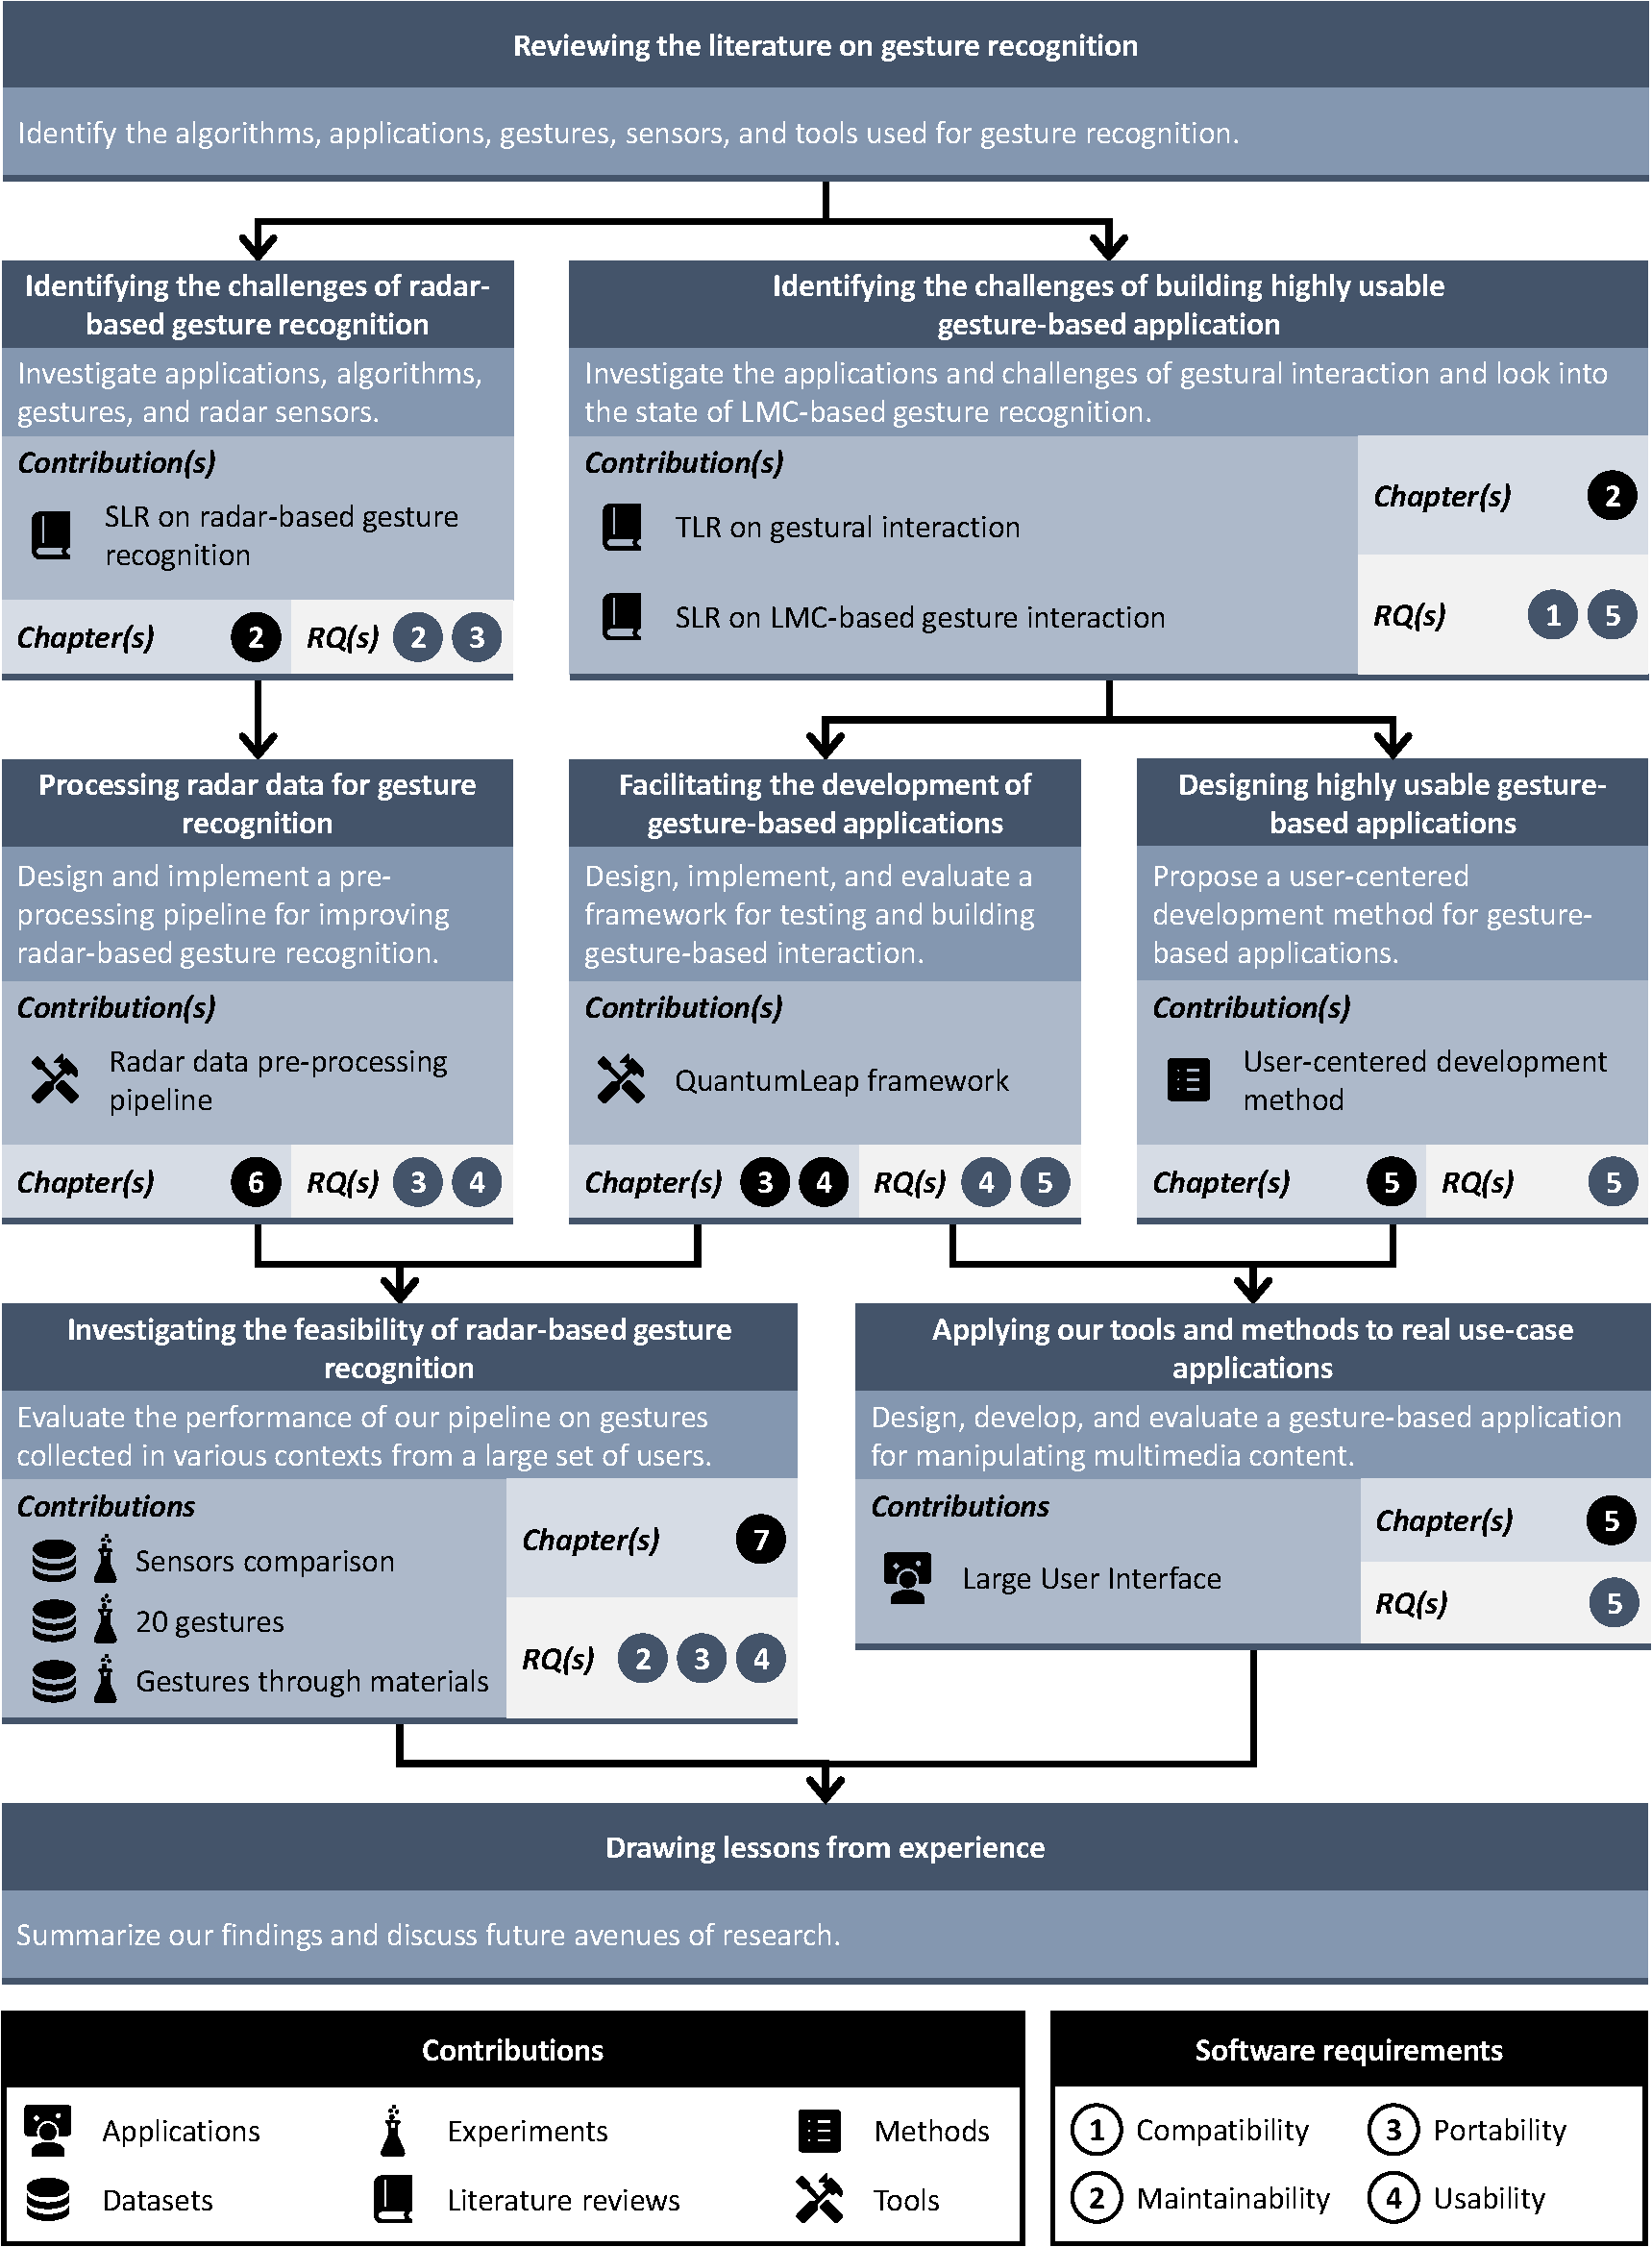
\includegraphics[width=\linewidth]{Figures/Introduction/graphical-summary.pdf}
    \vspace{-18pt}
    \caption{Overview of our research method. For each task, we provide the related contribution(s), chapter(s), and research question(s) (RQ).}
    \label{fig:graphical-summary}
\end{figure}

\chapter{State of the Art} \label{chap:state_of_the_art}

In this chapter, we explore the state of the art of gesture recognition in an attempt to answer the following research questions, defined in Section~\ref{sec:introduction:research:research-questions}:
\begin{itemize}
    \item [RQ1] \textit{What are the main challenges of mid-air gesture recognition?} %We investigate the main challenges faced by developers and practitioners in the development of gesture-based applications and discuss potential workarounds. -> conclusion
    \item [RQ2] \textit{What is the performance of radar sensors for mid-air gesture recognition?}
    \item [RQ3] \textit{What types of gesture-based applications would benefit from radar sensors?} %We take a look at existing radar-based gestural interfaces in the literature. -> conclusion
    \item [RQ5] \textit{How can tools and methods aid in designing gesture-based applications that operate independently of gesture recognition logic?}
\end{itemize}
\fig~\ref{fig:state_of_the_art:graphical-summary} highlights the main contributions of this chapter and how it fits into this thesis. The rest of the chapter is divided into four main parts.
Section~\ref{sec:state_of_the_art:overview} first provides an overview of gesture based-interaction. %, to address RQ1 and RQ5.
Section~\ref{sec:state_of_the_art:lmc} then takes a look at a relatively mature vision-based technology for hand gesture interaction, called the Leap Motion Controller (LMC), to contextualize the state of the research on radar-based gesture interaction, which is explored in Section~\ref{sec:state_of_the_art:radar}.
Finally, Section~\ref{sec:state_of_the_art:this_work} positions this work within the literature.

\begin{figure}
    \centering
    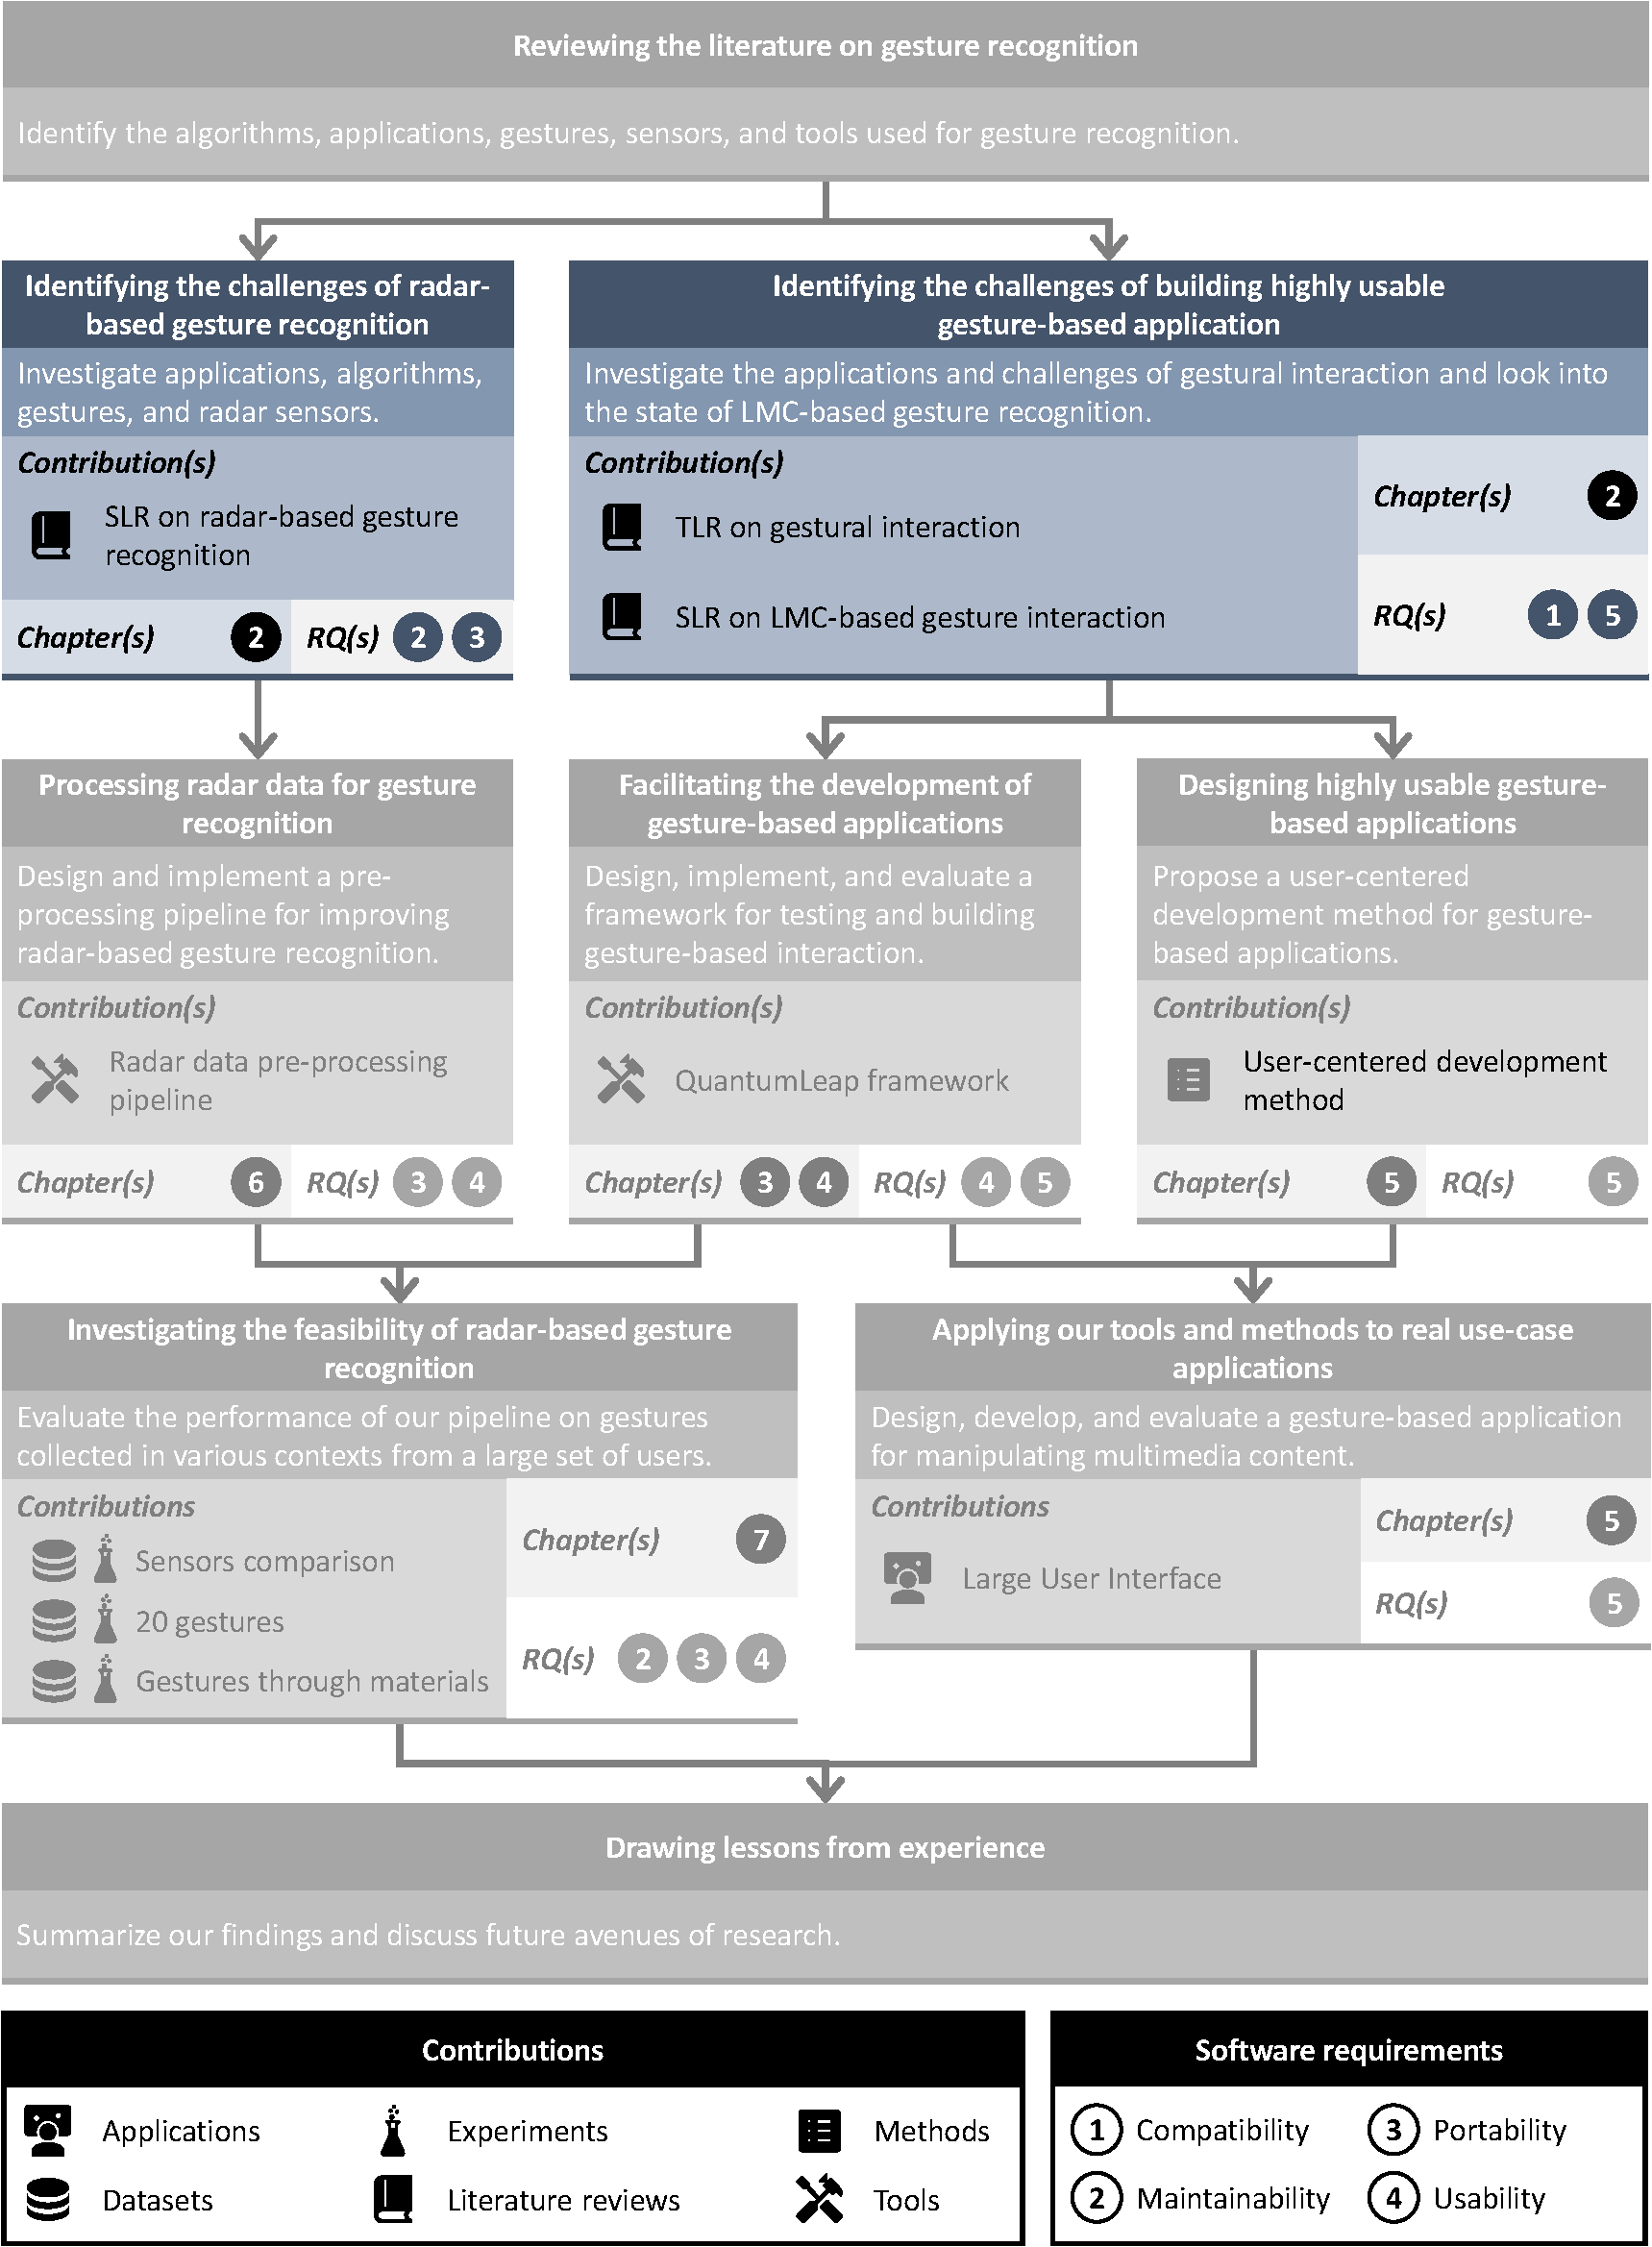
\includegraphics[width=\linewidth]{Figures/StateOfTheArt/graphical-summary-state-of-the-art.pdf}
    \vspace{-18pt}
    \caption{Main contributions of this chapter.}
    \label{fig:state_of_the_art:graphical-summary}
\end{figure}

\paragraph{Publications.} This chapter is based on three papers published in the EICS 2022 conference proceedings~\cite{Sluyters:2022:EICS}, Taylor and Francis IJHCI journal~\cite{Sluyters:2022:LUI} and ACM TiiS journal~\cite{Sluyters:2023}.

\paragraph{Resources.} The list of references from the two SLRs conducted in this chapter are available in an OSF repository at \url{https://osf.io/q43j8/?view_only=20b39a8a3d994ae4bd9ce52bfa2ded28}.



%================================================================================%
\section{Overview of Gesture-based Interaction} \label{sec:state_of_the_art:overview}
We conducted a Targeted Literature Review (TLR) to provide a summary of the literature on the topic of gesture-based interaction. TLRs are non-systematic, in-depth, and informative reviews of the literature that keep only the references maximizing rigorousness and relevance while minimizing selection bias~\cite{Kysh:2013}.
%
Section~\ref{sec:state_of_the_art:overview:ges} first looks into gesture elicitation studies (GES)~\cite{Wobbrock:2009}, which are a great way to involve end users in the development process of gesture-based applications. 
Section~\ref{sec:state_of_the_art:overview:challenges} then discusses the main challenges faced when building gesture interaction and Section~\ref{sec:state_of_the_art:overview:applications} provides examples of gesture-based interfaces in the literature.
Finally, Section~\ref{sec:state_of_the_art:overview:summary} summarizes our findings.

% %--------------------------------------------------------------------------------%
% \subsection{Applications} \label{sec:state_of_the_art:overview:applications}

% %--------------------------------------------------------------------------------%
% \subsection{Tools} \label{sec:state_of_the_art:overview:tools}
% % Frameworks, recognizers

% %--------------------------------------------------------------------------------%
% \subsection{Sensing Technologies} \label{sec:state_of_the_art:overview:sensors}
% IMUs
% Vision-based sensors (image vs. skeleton), google mediapipe hands, openpose
% Radars (fuse with next section?)
% Touch
% Smart gloves


%--------------------------------------------------------------------------------%
\subsection{Gesture Elicitation} \label{sec:state_of_the_art:overview:ges}
Involving end users in the development process of gesture-based applications, \eg by conducting a GES to identify a set of highly-guessable gestures, is crucial to provide a good user experience.
GESs were presented by Wobbrock \etal~\cite{Wobbrock:2009} as a participatory design method for understanding, collecting, exploring, and analyzing users preferences for gestures suitable to a particular context of use~\cite{Calvary:2003}, which is made up of a user, a device or computing platform, an environment, and some related tasks. The GES outcome consists of a characterization of users' gesture input behavior in terms of user-defined gestures~\cite{Grijincu:2014} with valuable information for designers, practitioners, and end users regarding the consensus levels between participants, computed as agreement or co-agreement scores~\cite{Vatavu:2014b}, or more recently agreement rates~\cite{Vatavu:2015}.
Vatavu and Zaiti~\cite{Vatavu:2014b} suggested that a correlation exists between the agreement rate and the recall rate, \ie a higher agreement usually means that participants recall their gesture propositions better.
This method has been widely applied to a large array of individual contexts of use (see~\cite{Villarreal:2020} for a systematic literature review), such as in Augmented Reality~\cite{Piumsomboon:2013}, smartphones~\cite{Ruiz:2011}, TVs~\cite{Vatavu:2014b,Morris:2012,Dong:2015}, and holograms~\cite{Pham:2018}.

The vast majority of these GESs target a single context of use, \ie a single category of users issuing gestures with a dedicated device in a given environment, thus posing the question of their transferability and applicability to other contexts. 
%
Among the few GESs targeting multiple contexts of use, Anthony \etal~\cite{Anthony:2013} observed that stroke gestures issued by a stylus \vs finger were inconsistent. In a systematic literature review of mid-air gestures, Groenewald \etal~\cite{Groenewald:2016} observed that gesture sets were largely inconsistent with each other and that no holistic study existed to address this problem.
%
Wittorf and Jakobsen~\cite{Wittorf:2016} elicited mid-air gestures for interacting with elements on wall displays. They noted that users' hand poses were often irrelevant to the meaning of the proposed gestures (\eg a \textit{swipe} gesture can be performed with any hand pose). Instead, the meaning was conveyed through the direction or expression of the gesture. When referents resembled actions associated with touch interactions, the proposed gestures were often larger-scale versions of common touch gestures. Users tended to favor gestures resembling the physical manipulation of objects. Overall, compared to other studies on smaller displays, the participants of this study proposed larger and more physically-based gestures.
%
Similarly, Ortega \etal~\cite{Ortega:2017} conducted a GES for eliciting multi-touch and mid-air gestures for 3D navigation in a procedurally generated universe. They found significant overlap between the proposed touch and mid-air gestures, and observed that most participants found mid-air gestures more immersive and intuitive than touch gestures.

Cross-context consistency has been initially addressed in three studies. Dingler \etal~\cite{Dingler:2018} designed a gesture set for reading via RSVP (Rapid Serial Visual Presentation) that ensures consistency across three devices, \ie a smartwatch, a smartphone, and smart glasses. A first GES collected gesture proposals for all three device types at once and considered the gesture proposals for all devices when constructing the final gesture set. They defined two new measures: the \textit{transferability score} (\ie how well a set of commands learned on one device can be ported to another) and the \textit{consistency score} (\ie the mean of all transferability scores between all devices). A second experiment with 18 participants validated the transferability of their gesture sets across devices. More recently, Vogiatzidakis and Koutsabasis~\cite{Vogiatzidakis:2019} computed a consistency rate $CR(C)$ by computing the agreement for one user performing one of 14 commands on seven home devices (\ie a smart television, speakers, video player, audio player, air conditioner, lights, and blinds). For this purpose, they computed the agreement rate for a single command and a single user, but for different devices. 
In the same home context of use~\cite{Vogiatzidakis:2020}, they introduced a consistency routine process that checks gesture proposals for consistency before incorporating them into a real system.

% In conclusion, apart from the three last studies, we are not aware of any work investigating gesture consistency, either in general or for mid-air interaction,  across different types of media objects. Some papers study users' preferred gestures either for a particular media type or for a well-defined set of actions, but independently of media types or without considering inter-media consistency. When consistency is addressed, it is across different device types, but not across different media types, which all have their generic and specific sets of functions. While recent work reported that gestures elicited on different devices are not consistent, previous work did not investigate how to ensure consistency across media types.


%--------------------------------------------------------------------------------%
\subsection{Challenges} \label{sec:state_of_the_art:overview:challenges}
This section highlights the main challenges that developers and practitioners may face in the development of gesture-based applications and discusses potential workarounds.


\subsubsection{Sensor Limitations} \label{sec:state_of_the_art:overview:challenges:sensors-limitations}
Depending on their technology, sensors may be subject to a series of limitations. For example, vision-based sensors such as the LMC are sensitive to environmental conditions~\cite{Yeo:2017}, limited field of view~\cite{Hayashi:2021}, occlusion~\cite{Brandon:2014}, and may raise privacy concerns~\cite{Avrahami:2018}. On the other hand, radar-based systems preserve privacy and can function in darkness, but are sensitive to clutter, noise, and interference. Some wearable sensors (\eg smart rings, watches, data gloves) may provide more accurate data, but this higher accuracy comes at the cost of practicality. Besides the limitations intrinsic to their technology, most sensors result in a compromise between a series of factors, including cost, field of view, framerate, and resolution.

Overall, practitioners should take all of these limitations into account in the design of their gesture-based user interfaces: gesture sets should be designed such that the sensor(s) can differentiate between each gesture and the selected sensor(s) should suit the context of use of the UI. If no single sensor suits the requirements of an application, a combination of two or more sensors (\eg the LMC and the MS Kinect~\cite{Marin:2014}) could be considered. 
%
\textbf{TODO - expand discussion on sensor fusion} Data fusion can benefits from different sensors 
Kalman filter (search for "data fusion kalman filter gesture recognition")


\subsubsection{Jitter} \label{sec:state_of_the_art:overview:challenges:jitter}
\label{sec:noise}
Jitter can be caused by tracking errors, sensor noise, or even a slight tremor in the user's hands. Too much jitter can significantly hinder interactions with gesture-based applications~\cite{Pavlovych:2009}, as it may induce recognition errors, as well as a lack of precision when pointing and selecting, especially on larger screens. It is thus important to perform at least some filtering in a gesture recognition pipeline to increase the precision of pointing and provide cleaner data to the gesture recognizers.

Depending on the sensors and recognition algorithms used, some filtering may already occur at several points in the pipeline. For instance, the LMC applies some filtering on the data that it provides~\cite{Colgan:2017}, and the sampling performed by some recognizers such as 3 cent~\cite{Caputo:2017}, Jackknife~\cite{Taranta:2017}, or \$P+~\cite{Vatavu:2017a} can act as a low pass filter. However, additional filtering may be applied to further smoothen the data.

Filters should be carefully selected and configured to provide reasonable smoothing while keeping latency low~\cite{Pavlovych:2009} and minimizing the risk of introducing inaccuracies. In \cite{Casiez:2012}, Casiez \etal propose the 1€ filter, a simple and fast filter based on double exponential smoothing that promises good smoothing and low latency for both fast and slow motion. They compare it to other filtering methods, namely, moving average, single and double exponential~\cite{LaViola:2003}, and Kalman, and show that it manages \textit{state-of-the-art} performance while being faster to execute.


\subsubsection{Gesture Production Variability} \label{sec:state_of_the_art:overview:challenges:production-variability}
Some variability in gesture production is usually observed both in gestures performed by a single user (intra-user variability) and by several users (inter-user variability). This variability can originate from differences in execution (\eg speed, trajectory) or in anatomy (\eg hand size, posture). If ignored, it can reduce gesture recognition accuracy and thus negatively impact the usability of gesture-based applications.

Several techniques exist to deal with gesture production variability. For instance, increasing the size of the training set by including more gesture samples produced by a greater range of users often results in higher recognition accuracy~\cite{Vatavu:2013}.
However, large training sets may increase execution time and are time-consuming to create. Synthetic data generation has been shown to increase accuracy while requiring little to no effort from developers~\cite{Taranta:2016, Leiva:2015}. A series of tools, such as MAGIC~\cite{Ashbrook:2010, Kohlsdorf:2011, Kohlsdorf:2013} and Gesture à Go Go~\cite{Leiva:2015}, have been developed to quickly augment gesture datasets with synthetic gestures. In~\cite{Maghoumi:2019}, Maghoumi and LaViola used synthetic gesture generation in their DeepGRU recognizer to avoid overfitting.

To increase accuracy for single users, recognizers could be trained only on gestures performed by this specific user. Indeed, template-matching algorithms have been shown to perform better in user-dependent settings~\cite{Vatavu:2013}, \ie where the recognizers are trained and tested with samples produced by the same user. 
Coupled with synthetic data generation, one could achieve high accuracy with little input from the target user. 

Finally, gesture recognition algorithms can be designed to accommodate some gesture production variability: for example, techniques such as Dynamic Time Warping (DTW) and spatial sampling can help deal with differences in gesture articulation speed~\cite{Taranta:2017, Vatavu:2013}.


\subsubsection{Static vs. Dynamic Gestures} \label{sec:state_of_the_art:overview:challenges:static-vs-dynamic}
Two main gesture types emerge from popular taxonomies: static and dynamic gestures~\cite{Aigner:2012,Vatavu:2008,Piumsomboon:2013,Choi:2014}. Inspired by~\cite{Vatavu:2008}, we propose the following definitions: a \textit{static} gesture is a particular configuration of the body or body parts at one instant of time, whereas a \textit{dynamic} gesture corresponds to a particular motion of the body or body parts through time. 
Different techniques may be leveraged to recognize each type of gesture. For instance, static gestures can be recognized at each frame to provide real-time recognition, while dynamic gestures are usually extracted from the raw stream of data (\ie gesture segmentation) before attempting to recognize them.


\subsubsection{Gesture Segmentation} \label{sec:state_of_the_art:overview:challenges:segmentation}
One of the greatest challenges in continuous gesture recognition is gesture segmentation, \ie extracting user gestures from a continuous stream of data. To maximize user satisfaction, a good gesture recognition pipeline should recognize all intentional gestures with minimal input from the user, while ignoring parasitic gestures (\eg transitions between gestures or unintentional motions)~\cite{Ashbrook:2010}. 

There are many different approaches to segmentation.
% 
A sliding window segmenter feeds the input data into a fixed-length buffer. The content of the buffer is continuously sent to the recognizer for evaluation. While this technique does not require input from the user, it makes assumptions about the length of gestures and relies on the recognizer to distinguish gestures from noise. Sliding windows have been used in combination with the 3 cent and Jackknife recognizers~\cite{Caputo:2019, Taranta:2017}. They have also been ML-augmented to distinguish intentional gestures from parasitic movements~\cite{Kratz:2016}. 
%
Segmentation may also be triggered by user input, \eg pressing a button performing a simple motion or hand pose to delimit gesture boundaries, or performing the gesture in a specific ``active'' zone in space. While accurate, these techniques require active input from the user and are thus likely to feel less natural to the user.
% 
Some publications have focused on using some properties of input data to trigger segmentation, such as speed and acceleration. For instance, in~\cite{Chen:2016}, Chen \etal used the energy and root mean square (RMS) of raw EMG signals to properly segment gestures (energy-based segmentation). 
%
Other techniques such as Machete~\cite{Taranta:2021} rely on simple recognizers that continuously evaluate input data to determine the possible boundaries of gestures.

The variability in gesture production discussed previously also impacts gesture segmentation. Consequently, DTW has been employed to accommodate differences in gesture articulation speed. 
%
For example, Hernández-Vela \etal~\cite{HernandezVela:2014} assumed that two consecutive motions were always separated by an idle gesture. They utilized DTW to detect this idle gesture, making it possible to extract user gestures from the continuous stream of data.
%
Instead of relying on idle gestures, Tang \etal~\cite{Tang:2018} opted for a different approach combining an SVM classifier with DTW for gesture segmentation. The SVM uses velocity information to detect ``slow-down zones'' occuring after a gesture has been performed and the DTW algorithm then backtracks to find the starting point of the gesture.

As gesture segmentation techniques are still far from perfect, some measures should be taken to limit the number of false positives. Examples include training recognition algorithms to recognize parasitic gestures (\eg by generating synthetic ``noise'' gestures)~\cite{Taranta:2017} and rejecting recognized gestures if their score falls below a threshold. This threshold may be arbitrarily defined or automatically computed based on the training set~\cite{Caputo:2019}.


\subsubsection{Overlapping Gestures} \label{sec:state_of_the_art:overview:challenges:overlapping-gestures}
Two gestures are overlapping when part of one gesture is identical to part of the other gesture. While well-designed overlapping gestures may lead to increased memorability~\cite{Roy:2013}, they are challenging to recognize as they rely on near-perfect gesture segmentation. Overlapping may occur between two gestures of one gesture set or between a gesture from the gesture set and a parasitic gesture (\eg typing on a keyboard or reaching for an object). In the first case, one can design the gesture set in such a way that each gesture is easily distinguishable from all other gestures. In the second case, the designer should take into account as many potential parasitic gestures as possible to reduce the risk of false positives. Tools such as Ashbrook \etal's MAGIC~\cite{Ashbrook:2010} assist designers in the creation of gesture sets with as little overlap as possible. GEsture Clustering toolKit (GECKo)~\cite{Anthony:2013} also helps investigate how end users articulate stroke gestures in terms of stroke number, order, and direction, thus assisting the designer in keeping or discarding a particular gesture to avoid overlapping.


% \subsubsection{Summary} \label{sec:state_of_the_art:overview:challenges:summary}

% The landscape of contactless UIs is constantly evolving. Sensors such as the LMC are paving the way towards cheap and accurate gesture recognition, while researchers are continuously working on improving gesture recognition algorithms.
% However, the lack of a common framework for gesture recognition is making it increasingly harder to keep track of this evolution outside of the research community, resulting in only a handful of real-life applications. 
% \ql aims at bridging the gap between researchers and developers by providing a common framework that helps researchers share the product of their research with the world and allows developers to write applications without spending time to solve the numerous challenges of gesture recognition.


\subsubsection{Arm Fatigue} \label{sec:state_of_the_art:overview:challenges:gorilla-arm}
Arm fatigue poses a significant challenge for mid-air gesture interaction, as badly designed gesture sets may reduce the time users can interact with a system before needing to rest~\cite{Hansberger:2017} or even lead to systems going unused~\cite{Siddhpuria:2017}. 

This phenomenon, often dubbed the ``gorilla arm effect'', has led to various metrics being proposed to quantify user arm fatigue. 
For instance, Hincapie \etal~\cite{Hincapie:2014} introduced the consumed endurance (CE) metric (Equation~\ref{eq:state-of-the-art:consumed-endurance}), calculated as the ratio between the interaction time and the endurance time of a participant (\ie the maximum duration they could sustain this type of interaction before having to rest their arm).
% 
\begin{equation}\label{eq:state-of-the-art:consumed-endurance}
    CE(T,TotalTime) = 100\frac{TotalTime}{E(T)}
\end{equation}
%
The authors demonstrated the applicability of this metric for assessing various design alternatives for gesture-based interfaces in a series of experiments.
For instance, they found that extending the arm and holding it higher consumed more endurance than holding it closer to the body and at a lower position. 
%
Jang \etal~\cite{Jang:2017} identified several limitations of the CE metric, including its oversight of rest periods and their impact on cumulative fatigue, its reliance on general assumptions regarding users' shoulder strength, and not applying well to interaction with low exertion levels. In response, they devised the three-compartment muscle (TCM) model, a more sophisticated model of muscle fatigue that addresses the limitations of the CE metric to quantify cumulative muscle fatigue with greater accuracy.

Hansberger \etal~\cite{Hansberger:2017} illustrated that well-designed mid-air gestures could achieve fatigue levels comparable to those experimented with traditional interaction methods, like a keyboard. Conversely, they found that gestures designed without considering arm fatigue could lead to high exhaustion levels, with many users unable to complete a 30-minute game session in an experiment they conducted.
%
Their study also suggested that the type of sensor used for gesture recognition could influence user fatigue. For instance, vision-based sensors like the LMC require users to place their hands within the field of view of the sensor, potentially leading to suboptimal hand position and thus increased fatigue, depending on the sensor placement. 
%
Wrist-worn IMUs, on the other hand, give users more flexibility in performing gestures. For example, Siddhpuria \etal~\cite{Siddhpuria:2017} demonstrated that ``at-your-side'' gestures recorded with a smartwatch enabled users to interact with public displays in a way that felt socially acceptable and natural while minimizing arm fatigue. 
Similarly, Liu \etal's Gunslinger~\cite{Liu:2015} relied on two LMCs mounted on users' tights, enabling them to adopt a more relaxed posture during interaction.


\subsubsection{Discoverability} \label{sec:state_of_the_art:overview:challenges:discoverability}
Due to their novelty, mid-air gesture interfaces have yet to be standardized \cite{Norman:2010}. Variations among users, whether personal or cultural, pose challenges in creating gesture-based UIs that feel natural and can be used seamlessly without prior introduction.

Given the considerable freedom afforded by gestures, designers must establish a clear conceptual model of the application, perhaps even more so than with traditional interfaces~\cite{Norman:2010}.
%
Possible actions should be easily discoverable, and clear tutorials and feedback mechanisms should be implemented to ensure that users can understand the physical constraints of the system (\eg limited field of view)~\cite{Norman:1999} and learn the proper gestures without feeling overwhelmed or frustrated~\cite{Norman:2010}. 
%
Signifiers, \ie deliberate or incidental cues about how an object is supposed to be used~\cite{Norman:2008}, should be placed by application designers in the UI to inform users about the potential actions available, and how to perform them. These cues should be subtle and seamlessly integrated into the interface to avoid distracting experienced users while remaining easy to notice and simple to understand for new users~\cite{Rovelo:2015,Walter:2013}.
%
Designers of gesture-based UI should also rely on existing conventions, such as those learned from touch-based UIs~\cite{Norman:1999}. For instance, swiping left to display the next page of a document may resonate with users familiar with touchscreens, as they have already adopted this convention for 2D gestures. 
%
While leveraging existing conventions may lower the entry barrier of mid-air gesture interfaces, designers must be cautious, as not all users share the same conventions (\eg liking content with a thumbs-up gesture \vs by drawing a checkmark). 
Similarly, designers should be careful when introducing new conventions to avoid overwhelming users with many unfamiliar gestures or violating existing conventions, which could lead to confusion. 
GESs can be a useful tool to identify existing conventions and define new conventions.

Discoverability is particularly important in public displays, where capturing and retaining user attention is challenging given that user patience can be low in such scenarios~\cite{Walter:2013}.
%
As such, researchers have explored various techniques for teaching gestures to users.
%
For example, Bau and Mackay~\cite{Bau:2008} and Kristensson and Denby~\cite{Kristensson:2011} investigated teaching 2D gestures on touchscreens by recognizing incomplete trajectories drawn by users and displaying possible continuations on the screen.
%
These systems were later extended to 3D mid-air interaction, covering simple 3D trajectories~\cite{Fennedy:2021} and gestures involving multiple body parts~\cite{Rovelo:2015, Alt:2018}. 
%
Walter \etal~\cite{Walter:2013} explored three strategies for revealing initial gestures on interactive public displays: spatial division (\ie displaying an explanation of the gesture on part of the screen), temporal division (interrupting the application to show the gesture in full screen), and integration (integrating visual cues in the application). They found that spatial division worked well, whereas temporal division caused users to leave while the cue was being shown because it interrupted their interaction with the application.
%
White \etal~\cite{White:2007} compared different methods for demonstrating to users how to interact with objects in AR. These methods included text (\ie a description of the gesture), diagrams (\ie an image of the gesture), and ghosting (\ie ghost images representing the action of the gesture). They found that combining two methods, such as text and ghosting, was preferred by users over using a single method.

% \textbf{TODO - citer article IJHCS discoverability scale}

\subsubsection{Gesture Set Customization}
Even a good gesture set might not satisfy everyone. Allowing users to customize gestures can result in higher memorability and usability over pre-designed gestures sets~\cite{Oh:2013,Nacenta:2013} and result in more inclusivity for users that suffer from some sort of disability.
% 
However, allowing customization comes with multiple challenges.
The gesture recognition pipeline must support custom gestures. Template-matching algorithms work well for that~\cite{TODO}, + mention deep learning that can be quickly trained.
Care should be given to design customization UI that is usable by everyone, in particular, people with a disability. Integrate this UI seamlessly into a gesture-based application.
How to represent gestures to users? Rather trivial with 2D gestures, Ok with 3d gestures, but what about radars and other sensors?

\textbf{TODO} %Template mùatching intrinsically supports customization. Some deeplearning can support that without complete retraining, but issues (catastrophic forgetting -> désapprendre des trucs pour apprendre ce qu'on lui ajoute) https://www.researchgate.net/publication/335698970_A_Study_on_Catastrophic_Forgetting_in_Deep_LSTM_Networks
%
\cite{Ouyang:2012} user-defined shortcuts (touch gestures). Allows to explore gestures from other users or even to identify potential meaning of the user gesture by comparing it with gestures from other users. Can reduce the time required to define custom gestures.
%
\cite{Xu:2022}

% Advantages over other gesture sets
% \cite{Oh:2013}
% \cite{Nacenta:2013}
% How to support them? Gesture recognizers,...
% How to  seamlessly into UI?
% How to represent gestures to users?



%--------------------------------------------------------------------------------%
\subsection{Applications} \label{sec:state_of_the_art:overview:applications}
In the field of 3D gesture interaction~\cite{LaViola:2013,Koutsabasis:2019}, hand gesture interaction (see ~\cite{Cheng:2016} for a survey) is particularly attractive as the hand is one of the most mobile human limbs. As such, many hand gesture-based interfaces have been proposed, in particular for interacting with large screens, such as TVs and public displays.

\subsubsection{Mid-air Gesture Interaction Techniques}
The research on mid-air gesture interaction revealed some of its shortcomings, including arm fatigue~\cite{Gupta:2017}, lack of consistency~\cite{Groenewald:2016}, and a need for short, pleasing, and easy-to-recognize gestures~\cite{Kohlsdorf:2013}. 
%
Several factors were identified that influence the quality of mid-air gestures on large displays, such as position and direction~\cite{Fruchard:2018}, sideways hand extension~\cite{Koutsabasis:2016}, dimension and bit cardinality~\cite{Vatavu:2013}, and continuity~\cite{Kohlsdorf:2013}. Beyond these factors, \cite{Nancel:2011} identified three factors for designing mid-air pan and zoom navigation on large displays: uni- \vs bimanual interaction, linear \vs circular motion, and level of guidance (from high guidance with a 1-dimension motion on an input device to low guidance with a free 3D motion in mid-air). They studied the impact of these factors on users' performance and subjective preference by comparing 12 mid-air pan-and-zoom techniques with various factor combinations. Despite its appeal, free mid-air motion was less efficient and more tiring than other techniques. Overall, users preferred linear motion and bimanual interaction over other techniques.
%
Various techniques for mid-air interaction with large screens have been studied in the literature to try to alleviate these shortcomings, but papers often focus on a few actions only, such as point-and-click or pan-and-zoom~\cite{Nacenta:2013}, or a limited set of gestures~\cite{Groenewald:2016}.

For instance, Yoo \etal~\cite{Yoo:2015} compared two techniques for interacting with large displays: point and dwell and a combination of push and grab-and-pull. When navigating Twitter feeds on a public display using a Microsoft Kinect for gesture recognition, the combination of push and grab-and-pull gestures was deemed more fun, faster, and less tiring than point-and-dwell.

Vogel and Balakrishnan~\cite{Vogel:2005} compared different techniques for freehand pointing and selecting a target on a large display, including two clicking techniques (airtap and thumb trigger) and three pointing techniques (ray casting, relative pointing with clutching, and hybrid ray-to-relative pointing). Auditory and visual feedback was implemented to compensate for the lack of tactile feedback inherent to mid-air gestural interfaces. Although clicking techniques were equally performant and accurate, airtap induced less fatigue than thumb trigger. Participants preferred relative pointing with clutching for pointing, as it felt faster and easier to perform.


\subsubsection{Interaction with Multimedia Objects}
The consumption and manipulation of multimedia objects, such as audio, video, pictures, and documents, is popular in public and private spaces, both on large displays (\eg TVs, public displays) and small screens (\eg smartphones, tablets). 
%
As such, enabling gesture-based interaction with multimedia objects is a relevant research subject in HCI, with works usually focusing on only one or two media types at a time.

% More specifically for mid-air interaction with multimedia objects, less work can be found and usually focus on one media type or two at a time but not as a whole: images~\cite{Koutsabasis:2016}, videos~\cite{Zigelbaum:2010}, virtual objects~\cite{Caputo:2015}, 3D travel~\cite{Ortega:2017}, images and videos~\cite{Drossis:2013}.
For example, Ackad \etal~\cite{Ackad:2015} designed and evaluated a \textit{media ribbon}, a large public display that shows information about events for theaters and concerts. Designing an intuitive and easy-to-learn gestural interface is crucial for such displays, as people are less inclined to take time to learn how to interact. They evaluated the interface by letting passers-by freely interact with the large display and interviewing them afterward. They suggested keeping gesture sets small and easy to learn, \eg by always displaying the most important gestures and by providing context-dependent tutorials for additional gestures.

Vlaming \etal~\cite{Vlaming:2008} designed a system for interacting with documents, videos, and pictures on a large screen through a combination of pointing and pinch gestures. A modified Wiimote and an infrared light source tracked two retro-reflective points per hand (index and thumb). Multiple objects could be displayed simultaneously and manipulated through one- and two-handed gestures. Active objects could be controlled in various ways by interacting with media-dependent widgets. The authors observed that the system caused arm fatigue after prolonged use and that the use of two-handed gestures was sometimes misunderstood. 

Zigelbaum \etal's G-stalt~\cite{Zigelbaum:2010} relied on an advanced motion capture system to track retro-reflective dots on each hand. A set of 21 gestures allowed users to manipulate and re-organize multimedia content in a 3D space. The authors recommended designing gestural interfaces to be neither too complex nor too simple and taking advantage of the hands' capabilities while keeping gestures easy to learn and perform.

Jakobsen \etal~\cite{Jakobsen:2015} compared touch and mid-air gestures for object selection on large displays. They observed that touch was usually faster and more accurate than mid-air gestures, but that this advantage decreased with the distance between objects, as mid-air gestures allowed users to see and interact with targets anywhere on the screen with minimal motion. The poor performance of mid-air gestures could be explained in part by an imperfect implementation of the system. They also showed that users mostly favored mid-air gestures when regularly forced to move away from the screen (\eg to interact with something else), despite the loss in accuracy incurred.

Siddhpuria \etal~\cite{Siddhpuria:2017} designed \textit{at-your-side} gestures, \ie gestures performed with the arm at rest along the side of the body, to minimize the effort associated with typical mid-air gesture interaction. \textit{At-your-side} were considered as low-effort and low embarrassment by users, and thus suited for interaction with (semi-)public displays.

Drossis \etal~\cite{Drossis:2013} proposed MAGIC, a system for browsing a collection of pictures and videos on a large display in public spaces with mid-air gestures captured by a Microsoft Kinect. They observed that fine-grained gestures suffered from low recognition accuracy at a distance and thus replaced them with a combination of buttons and point-and-dwell.

%--------------------------------------------------------------------------------%
\subsection{Summary} \label{sec:state_of_the_art:overview:summary}
Designing good gesture-based interfaces is a challenging endeavor in which user preferences often find themselves at odds with the technical challenges of gesture-based interaction. Finding a balance between usability and addressing these technical challenges should be possible, although it requires a high level of expertise in UX design, application development, and gesture recognition. This high barrier of entry and the lack of tools available to aid developers in this process partly explain why 3D gesture-based recognition is still relatively niche, despite its potential benefits to many facets of society.


%================================================================================%
\section{Analysis of a Mature Sensing Technology} \label{sec:state_of_the_art:lmc}
Looking at more mature sensing technologies, such as vision-based sensors, can help us better grasp the challenges of radar-based gesture interaction.
%
In this section, we chose to focus on the Leap Motion Controller (LMC): an innovative, 3D motion-capturing device designed to track two hands and their fingers~\cite{Togootogtokh:2018} with high precision and robustness~\cite{Weichert:2013}. Its API transforms the raw data from its two near-infrared cameras into a hand skeleton to be used in any application. The LMC reaches sub-millimeter (0.2 mm) accuracy for static gestures and falls to 1.2 mm for dynamic gestures~\cite{Weichert:2013}. It natively recognizes a handful of system-defined gestures but custom gesture recognition algorithms are often preferred as they enable the support of a wider range of gestures~\cite{Brandon:2014}.
The affordability, off-the-shelf availability, and accuracy of the LMC make it relatively popular among researchers and practitioners.

We undertook a Systematic Literature Review (SLR)~\cite{Kitchenham:2010} to explore the algorithms employed for LMC-based gesture recognition (\fig~\ref{fig:state_of_the_art:lmc:prisma}). 
%
The query \texttt{RQ=``leap motion'' AND ``gesture recognition''} was run in the ACM Digital Library\footnote{Accessible at \url{https://dl.acm.org}}, which was highlighted as a good option for computer science literature reviews by Gusenbauer and Haddaway~\cite{Gusenbauer:2020}. Leveraging only one extensive database of papers provided us with a good overview of the literature on LMC-based gesture recognition while allowing us to channel most of our efforts into our subsequent SLR on radar-based gesture recognition (Section~\ref{sec:state_of_the_art:radar}).
%
The query yielded 390 publications, from which $N{=}43$ were identified as relevant. 

\begin{figure}[htb]
    \centering
    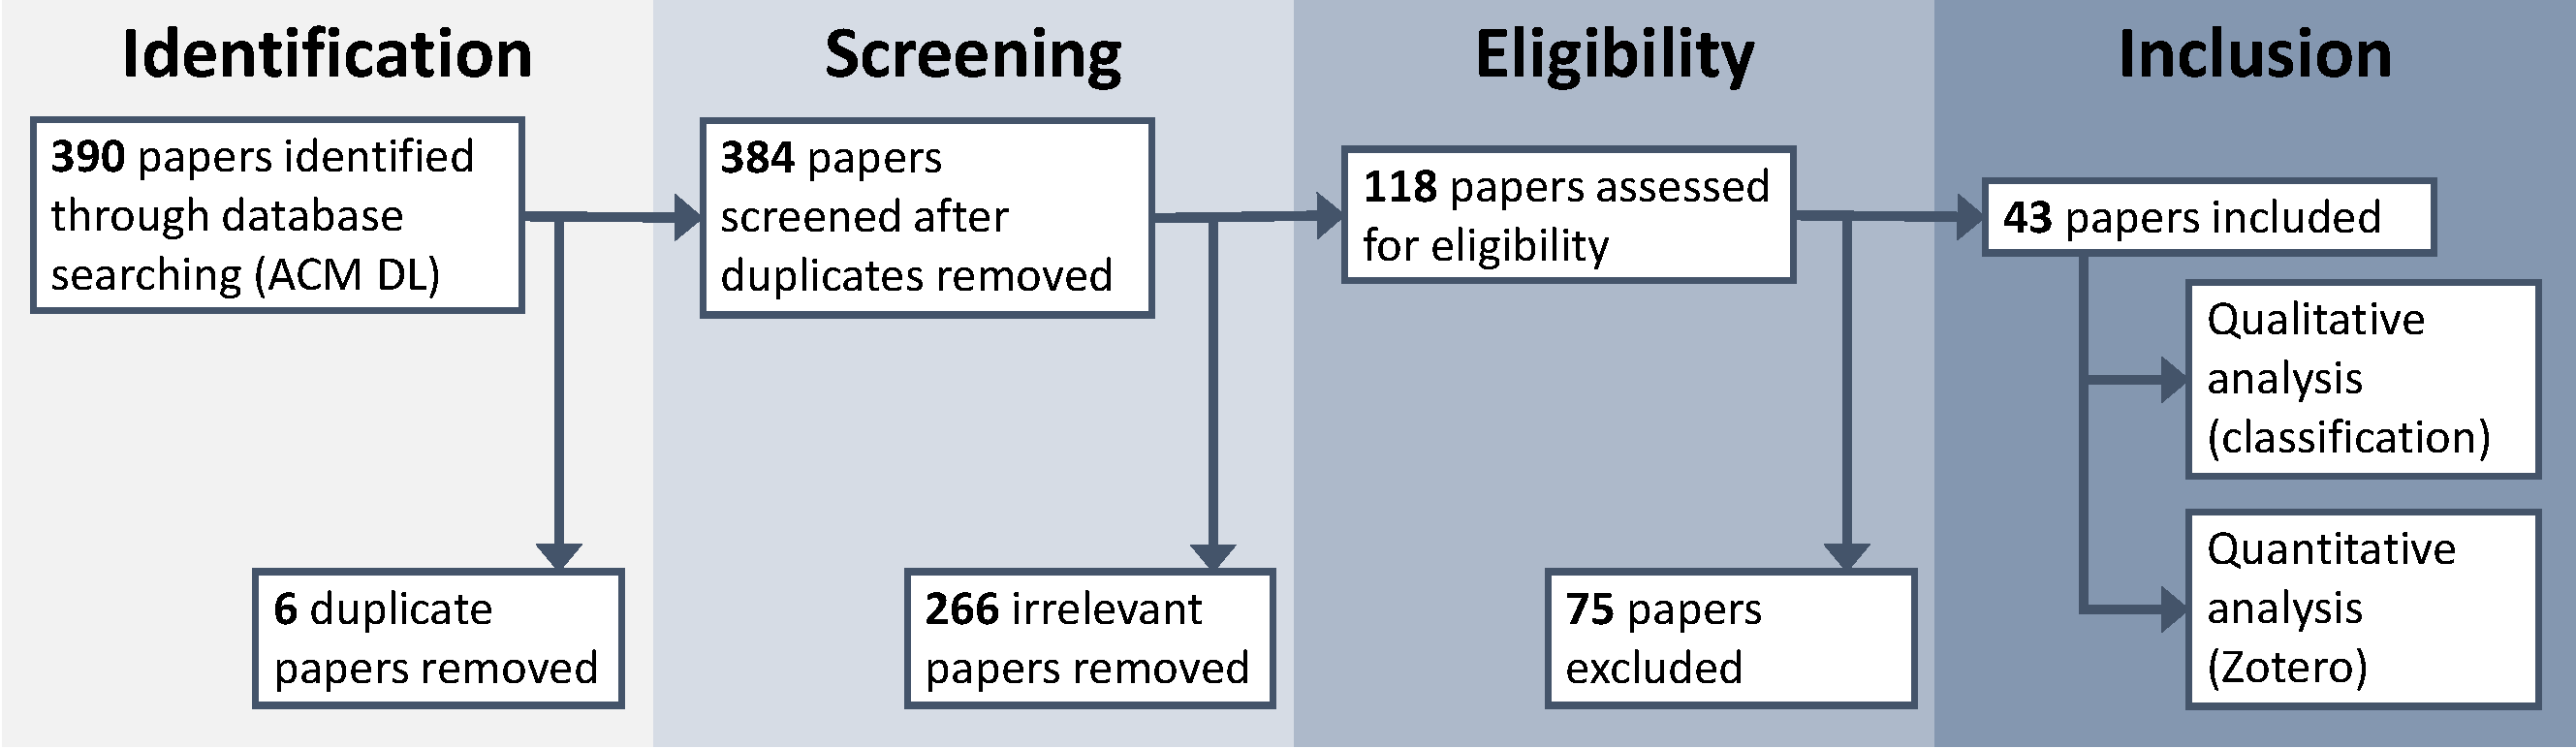
\includegraphics[width=\linewidth]{Figures/StateOfTheArt/LMC/PRISMA-LMC.pdf}
    \vspace{-18pt}
    \caption{PRISMA diagram~\cite{Page:2021} of our SLR on LMC gesture recognition.}
    \label{fig:state_of_the_art:lmc:prisma}
    \vspace{-8pt}
\end{figure}

\subsection{Algorithms} \label{sec:state_of_the_art:lmc:algorithms}
22 types of algorithms for gesture recognition were identified in the papers, spanning across seven categories (\tab~\ref{tbl:state_of_the_art:lmc:algorithms}).

\begin{table}[hbt]
    \resizebox{\columnwidth}{!}{
    \begin{tabular}{lll}
        \toprule
        \textbf{Type} & \textbf{Algorithm} & \textbf{References} \\
        \midrule
        Opportunistic & Hard-Coded Thresholds & \cite{Cai:2019,Caputo:2015,Fu:2016,Galea:2018,Sadik:2017,Theofanidis:2017,Tran:2016,Yang:2017,Yao:2017,Yu:2018,Zhou:2018b} \\
         & Leap Gestures & \cite{Caputo:2015,Chatterjee:2015,Daniels:2014,Liang:2017,Mendez:2018,Sadik:2017,Theofanidis:2017,Tran:2016,Yao:2017,Zocco:2015} \\
         & GameWAVE Software & \cite{Liang:2017} \\
        \midrule
        Nearest Neighbor & K-Nearest Neighbors & \cite{Caputo:2017,Chiang:2017,Clark:2016,Daniels:2014,Filho:2018,GomezDonoso:2017,Li:2019,Taranta:2017,Thaweesitthichat:2018,Stinghen:2018} \\
        \midrule
        Support Vector Machines & Support Vector Machine & \cite{Ferreira:2019,Filho:2018,Stinghen:2018,Jiang:2018,Kiselev:2019,Lopez:2015,Marin:2016,Park:2019,Simos:2016} \\
        \midrule
        Neural Networks & Multilayer Perceptron & \cite{Mapari:2016,Togootogtokh:2018} \\
         & Deep Feedforward Neural Network & \cite{Schioppo:2019} \\
         & Feedforward Neural Network & \cite{DePrisco:2016} \\
         & Gated Recurring Units & \cite{Thaweesitthichat:2018} \\
         & Neural Network & \cite{Jiang:2018} \\
         & Radial Basis Function Network & \cite{Zeng:2018} \\
        \midrule
        Hidden Markov Models & Hidden Markov Model & \cite{Kumar:2017a,Kumar:2018,Volioti:2018,Zou:2017} \\
         & Coupled Hidden Markov Model & \cite{Kumar:2017b} \\
        \midrule
        Ensemble Learning & Random Forest & \cite{Marin:2016,Schioppo:2019} \\
         & Bagging Trees & \cite{Jiang:2018} \\
         & Gradient Tree Boosting & \cite{Kiselev:2019} \\
        \midrule
        Other AI/ML Techniques & Decision Tree & \cite{Filho:2018,Stinghen:2018,Zhou:2018b} \\
         & Decision Table & \cite{Li:2017c} \\
         & Linear Discriminant Analysis & \cite{Jiang:2018} \\
         & Fuzzy Integral & \cite{Li:2017c} \\
         & Multinomial Logistic Regression & \cite{Kiselev:2019} \\
         & Naive Bayes & \cite{Preventis:2014} \\
        \bottomrule
    \end{tabular}
    }
    \caption{Summary of the gesture recognition algorithms identified in the SLR.}
    % \vspace{-20pt}
    \label{tbl:state_of_the_art:lmc:algorithms}
\end{table}

A major part of the analyzed publications ($\frac{16}{43}{=}37\%$) implemented gestural support opportunistically, \ie by relying on the few system-defined gestures natively supported by the LMC or by recognizing gestures based on hard-coded thresholds (\eg \cite{Cai:2019,Galea:2018,Zhou:2018b}). While this opportunistic approach may be appropriate in some cases (\eg for quick prototyping\cite{Anthony:2012} or very simple UIs), it often forces developers to make significant compromises that could be avoided with more advanced recognition techniques. For instance, Liang \etal~\cite{Liang:2017} designed a storytelling system in which children can interact with hand gestures, but these gestures were hard-coded and could not be modified easily to better fit the motor abilities and preferences of each child. Zocco \etal\cite{Zocco:2015} showed that an LMC-based system could be more efficient than the traditional trackpad-keyboard combination to interact with a Command and Control system. However, as they were limited to the few gestures natively supported by the LMC, they did not study whether more suitable types of gestures could result in even greater efficiency and better usability, such as those obtained with user-defined gestures~\cite{Grijincu:2014}.

Found in nine references ($\frac{9}{43}{=}21\%$), K-Nearest Neighbors (KNN) classifiers~\cite{Duda:2000} were also a popular choice for gesture recognition. These algorithms are a simple yet powerful alternative to the opportunistic approach as they are easy to implement and train while being reasonably fast and accurate. Some are presented as all-purpose recognizers \cite{Caputo:2017,Taranta:2017} while others target more specific applications such as handwritten numerals recognition \cite{Chiang:2017} and Sign Language recognition, which remains a key topic for any language: American~\cite{Ferreira:2019,Kumar:2017b,Mapari:2016,Schioppo:2019}, Greek~\cite{Simos:2016}, and Thai~\cite{Thaweesitthichat:2018}.

The remainder of the papers featured more advanced ML techniques such as Neural Networks (NNs), Support Vector Machines (SVMs), Hidden Markov Models (HMMs), or Ensemble Learning. These techniques were used in all kinds of applications. For instance, Simos and Nikolaos~\cite{Simos:2016} used an SVM to classify the 24 letters of the Greek Sign Language alphabet with high accuracy, and Kumar \etal~\cite{Kumar:2017a} trained an HMM to recognize words from single-stroke Latin sentences.

Among the 27 publications relying exclusively on non-opportunistic algorithms for gesture recognition, only four ($\frac{4}{27}{=}14.8\%$) targeted both static and dynamic gestures, while the rest focused exclusively on one type of gesture.

Finally, some papers combined algorithms and/or sensors. Daniels \etal~\cite{Daniels:2014} combined the LMC's native gestures with Wobbrock \etal's \$1 recognizer~\cite{Wobbrock:2007} to recognize a larger set of gestures for the manipulation of protein structures. Jiang \etal~\cite{Jiang:2018} combined an LMC with myography data, Marin \etal augment the LMC with an MS Kinect~\cite{Marin:2014} or a depth sensor~\cite{Marin:2016} to increase accuracy. 

%--------------------------------------------------------------------------------%
\subsection{Summary} \label{sec:state_of_the_art:lmc:summary}
Despite the popularity and ease of use of the LMC, we observe that none of the papers discussed in the previous section attempted to propose an approach that is reusable across gesture sets, gestural UIs, and applications towards their mainstream development. Reusability, interoperability, and maintainability, three important (sub-)factors for software quality defined in the ISO/IEC 25010~\cite{iso25010}, are not explicitly addressed.


%================================================================================%
\section{A Deep Dive into Radar-based Gesture Interaction} \label{sec:state_of_the_art:radar}

To get a comprehensive look at the state of the research on radar-based gesture interaction, an SLR was conducted to identify the types of radar, algorithms, and gesture sets used for radar-based gesture recognition (\fig~\ref{fig:state_of_the_art:radar:prisma}). The query \texttt{RQ=``radar'' AND ``gesture recognition''} was run in five digital libraries: (1) \href{https://dl.acm.org/}{ACM Digital Library}, (2) \href{https://ieeexplore.ieee.org/Xplore/home.jsp}{IEEE Xplore}, (3) \href{https://www.mdpi.com/journal/sensors}{MDPI (Sensors)}, (4) \href{https://link.springer.com/}{SpringerLink}, and (5) \href{https://www.sciencedirect.com/}{Elsevier ScienceDirect} and resulted in 1,515 articles, from which $N=118$ were identified as relevant. \tab~\ref{tab:state_of_the_art:radar-slr-references} groups these papers based on their year of publication. 91.5\% of the papers were published between 2018 and 2020, indicating that this field of research has recently become quite active. 

\begin{figure}[hbt]
    \centering
    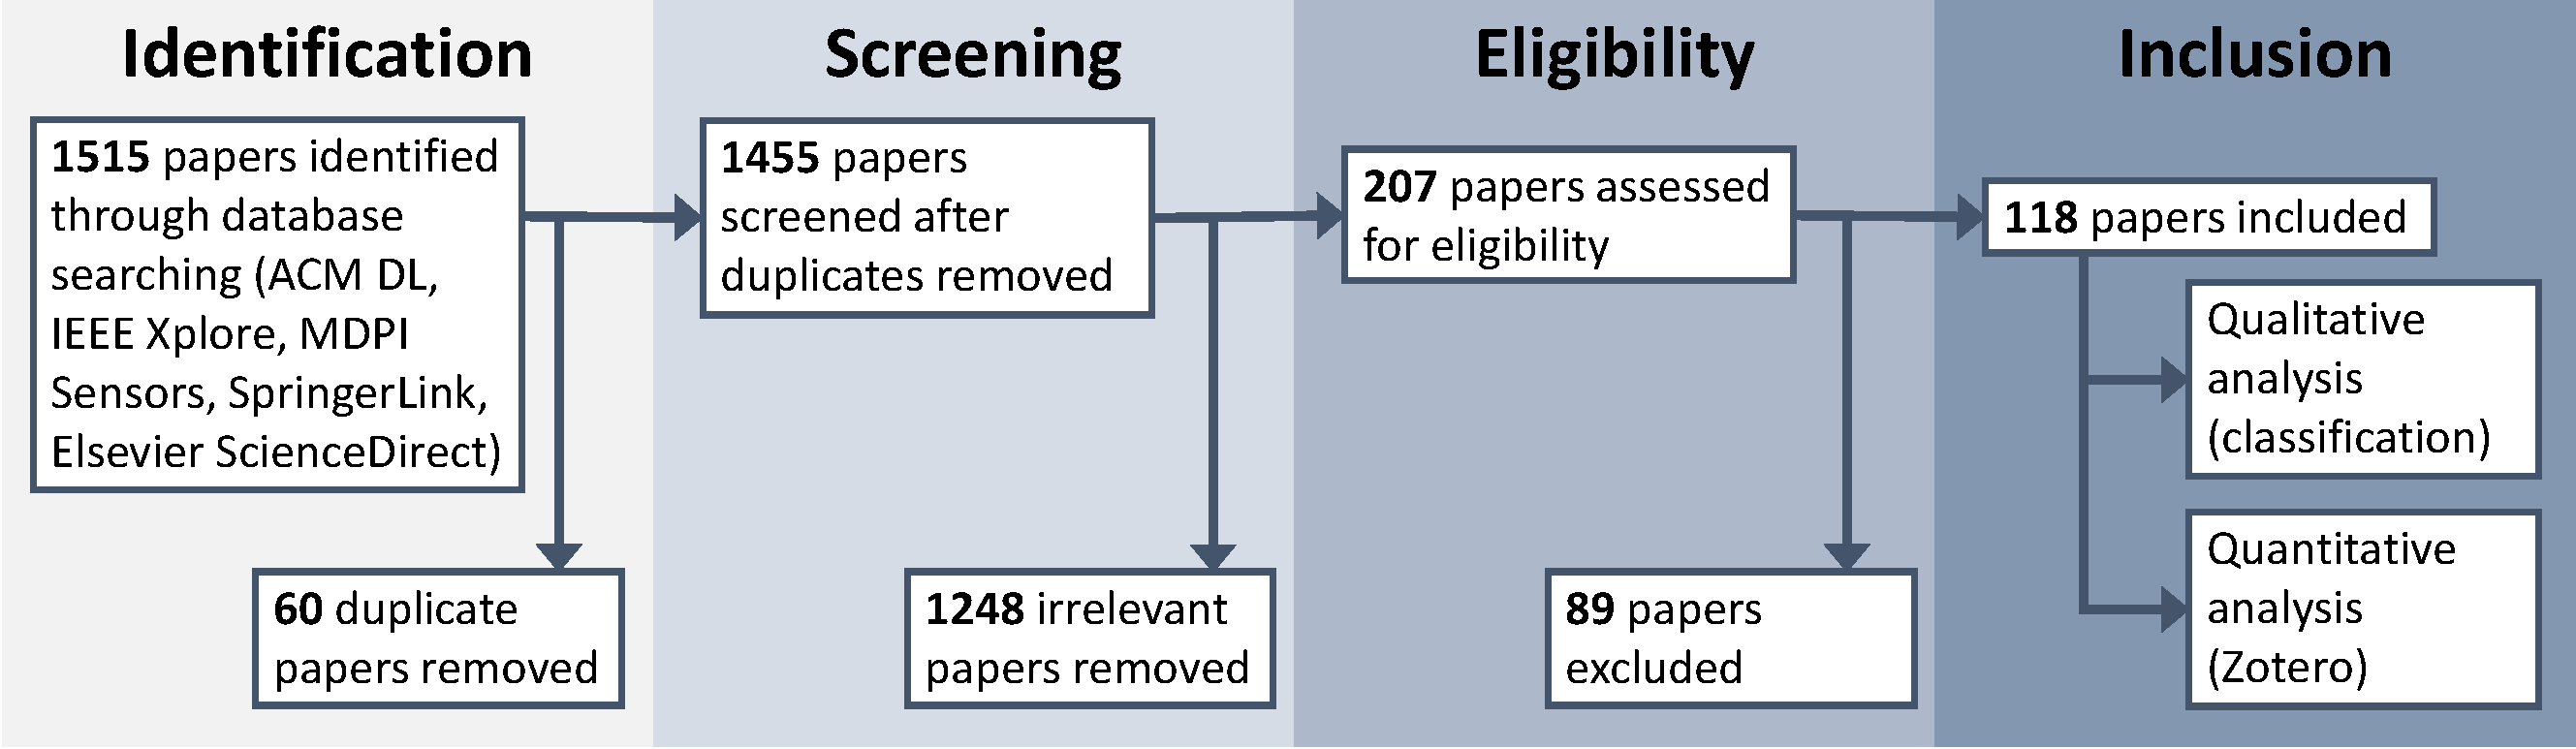
\includegraphics[width=\linewidth]{Figures/StateOfTheArt/Radar/PRISMA-Radar.pdf}
    % \vspace{-18pt}
    \caption{PRISMA diagram~\cite{Page:2021} of our SLR on radar-based gesture interaction.}
    \label{fig:state_of_the_art:radar:prisma}
    % \vspace{-8pt}
\end{figure}

\begin{table}[hbt]
    \footnotesize
    \begin{tabular}{crp{.78\textwidth}}
        \toprule
        \textbf{Year} & \textbf{\#Refs} & \textbf{Reference(s)} \\
        \midrule
        2009 & 1 & \cite{Li:2009} \\
        2014 & 1 & \cite{Wan:2014} \\
        2015 & 1 & \cite{Molchanov:2015} \\
        2016 & 6 & \cite{Kim:2016,Lien:2016,Malysa:2016,Park:2016,Wang:2016,Zhang:2016} \\
        2017 & 11 & \cite{Lan:2017,Li:2017a,Mcintosh:2017,Ritchie:2017,Sakamoto:2017,Viunytskyi:2017,Zhang:2017,Kim:2017b,Kim:2017a,Dekker:2017,Khan:2017} \\
        2018 & 21 & \cite{Hazra:2018,Ishak:2018,Lan:2018b,Lan:2018a,Li:2018b,Li:2018a,Lou:2018,Nguyen:2018a,Nguyen:2018b,Patra:2018,Ryu:2018,Sakamoto:2018,Smith:2018,Suh:2018,Sun:2018,Yang:2018,Zhang:2018d,Zhang:2018a,Zhang:2018b,Zhang:2018c,Zhou:2018a} \\
        2019 & 35 & \cite{Ahmed:2019,Amin:2019b,Amin:2019a,Arsalan:2019,Arthamanolap:2019,Berenguer:2019,Chen:2019,Choi:2019,Copic:2019,Du:2019,Eggimann:2019,Ehrnsperger:2019,Feng:2019,Fhager:2019,Ghaffar:2019,Gigie:2019,Goswami:2019,Hazra:2019b,Hazra:2019a,Kang:2019,Kulhandjian:2019,Liu:2019,Skaria:2019,Sun:2019,Wang:2019f,Wang:2019a,Wang:2019b,Wang:2019c,Wang:2019d,Wang:2019e,Zhang:2019d,Zhang:2019a,Zhang:2019b,Zhang:2019c,Zhao:2019} \\
        2020 & 41 & \cite{Ahmed:2020,Amin:2020,Bannon:2020,Du:2020,Ehrnsperger:2020,Gurbuz:2020,Kern:2020,Khan:2020,Lee:2020,Leem:2020b,Leem:2020a,Li:2020b,Li:2020a,Liang:2020,Liu:2020b,Liu:2020a,Miller:2020,Park:2020,Ren:2020,Ritchie:2020,Rozman:2020,Santhalingam:2020b,Santhalingam:2020a,Skaria:2020b,Skaria:2020a,Sun:2020b,Sun:2020a,Tzadok:2020,Vandersmissen:2020,Wang:2020d,Wang:2020a,Wang:2020b,Wang:2020c,Wu:2020,Xia:2020,Yu:2020b,Yu:2020a,Zeng:2020b,Zeng:2020a,Zhang:2020b,Zhang:2020a} \\
        2021 & 1 & \cite{Ahmad:2021} \\
        \bottomrule
    \end{tabular}
    \caption{Distribution of papers from our systematic literature review, based on their year of publication.}
    \label{tab:state_of_the_art:radar-slr-references}
    % \vspace{-14pt}
\end{table}

%--------------------------------------------------------------------------------%
\subsection{Applications} \label{sec:state_of_the_art:radar:applications}
While all papers provided some evaluation of the system performance (see \fig~\ref{fig:state_of_the_art:radar:validation-type}), only 14 papers ($\frac{14}{118}{=}12\%$) demonstrated potential use cases of their system with a prototype and one paper ($\frac{1}{118}{=}1\%$) evaluated the user experience of the proposed system.

\begin{figure}[hbt]
    \centering
    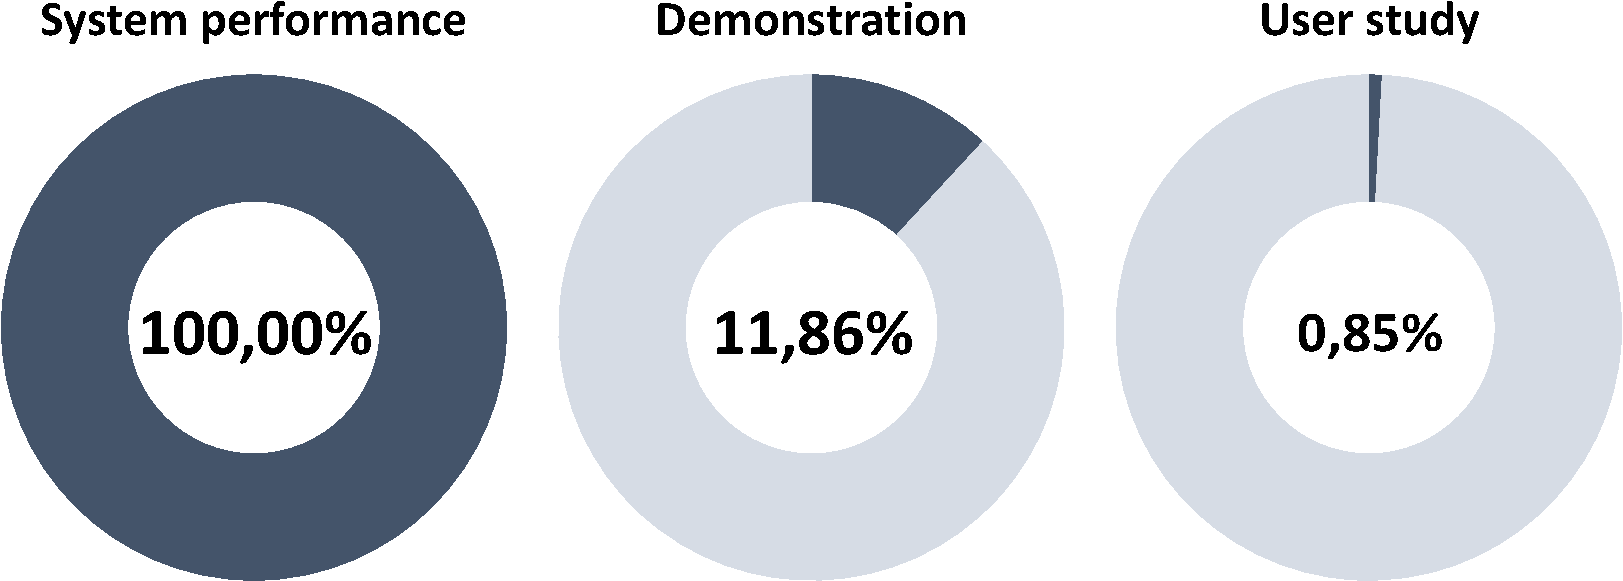
\includegraphics[height=2.6cm]{Figures/StateOfTheArt/Radar/evaluation-type.pdf}
    % \vspace{-10pt}
    \caption{Types of validation.}
    \label{fig:state_of_the_art:radar:validation-type}
%    \vspace{-6pt}
\end{figure}


Eight of the 14 papers focused on multimedia applications, including controlling media playback (\eg music, videos)~\cite{Du:2019,Lee:2020,Wu:2020,Smith:2018,Liu:2020b} or triggering specific keystrokes (\eg Enter, Alt+F4)~\cite{Nguyen:2018a,Nguyen:2018b}, thus enabling the control of classical PC applications without modifications to their source code.
Liu \etal~\cite{Liu:2020b} introduced \textit{mHomeGes}, a radar-based gesture recognition system for smart homes that allowed users to control lighting, music, and a home monitor. After evaluating the user experience of the system, the authors observed that 70\% of the users found \textit{mHomeGes} more convenient than voice commands.
Smith \etal~\cite{Smith:2018} implemented in-vehicle interaction for the driver and passengers of a car to control music and answer phone calls.
Lien \etal~\cite{Lien:2016} introduced \textit{virtual tookits}, \ie small sets of gestures complex enough to enable the control of UIs while being memorable and easy for the system to recognize. They built a pipeline based on the Google Soli radar to recognize gestures in real-time and trigger actions in applications accordingly.
Wu \etal~\cite{Wu:2020} proposed to embed radar antennas into fabric to augment everyday objects (\eg furniture, clothing) with gesture-based interfaces. The authors developed prototypes to demonstrate various use cases, including controlling media playback with an interactive sofa armrest, checking fitness goals with interactive sports clothing, and creating interactive plush toys.

Other applications included air-writing recognition~\cite{Wang:2020a}, user authentication based on 2D hand trajectories and breathing patterns~\cite{Leem:2020b}, making a home-assistant for people with hearing impairements~\cite{Santhalingam:2020b}, manipulating medical images in an operating room~\cite{Miller:2020}, and controlling a robot with hand gestures~\cite{Zhang:2020a,Li:2009}.

%--------------------------------------------------------------------------------%
\subsection{Algorithms} \label{sec:state_of_the_art:radar:algorithms}

\fig~\ref{fig:state_of_the_art:radar:algorithms} presents the algorithms used in our corpus.
151 algorithms for radar-based gesture recognition were identified, the majority representing deep learning approaches ($\frac{81}{151}=54\%$), of which Convolutional Neural Networks (CNNs) were the most frequently used.
CNNs were often combined with other models, such as Long Short-Term Memory (LSTM) or Support Vector Machines (SVM), in $\frac{23}{158}=15\%$ of the cases.
Classical machine learning algorithms were still used, as follows: K Nearest Neighbors ($\frac{23}{151}=15\%$), Support Vector Machines ($\frac{16}{151}=11\%$), ensemble learning ($\frac{8}{151}=5\%$), Decision Trees ($\frac{6}{151}=4\%$), Hidden Markov Models ($\frac{3}{151}=2\%$), and Bayesian networks ($\frac{2}{151}=1\%$). 

\begin{figure}[t]
    \centering
    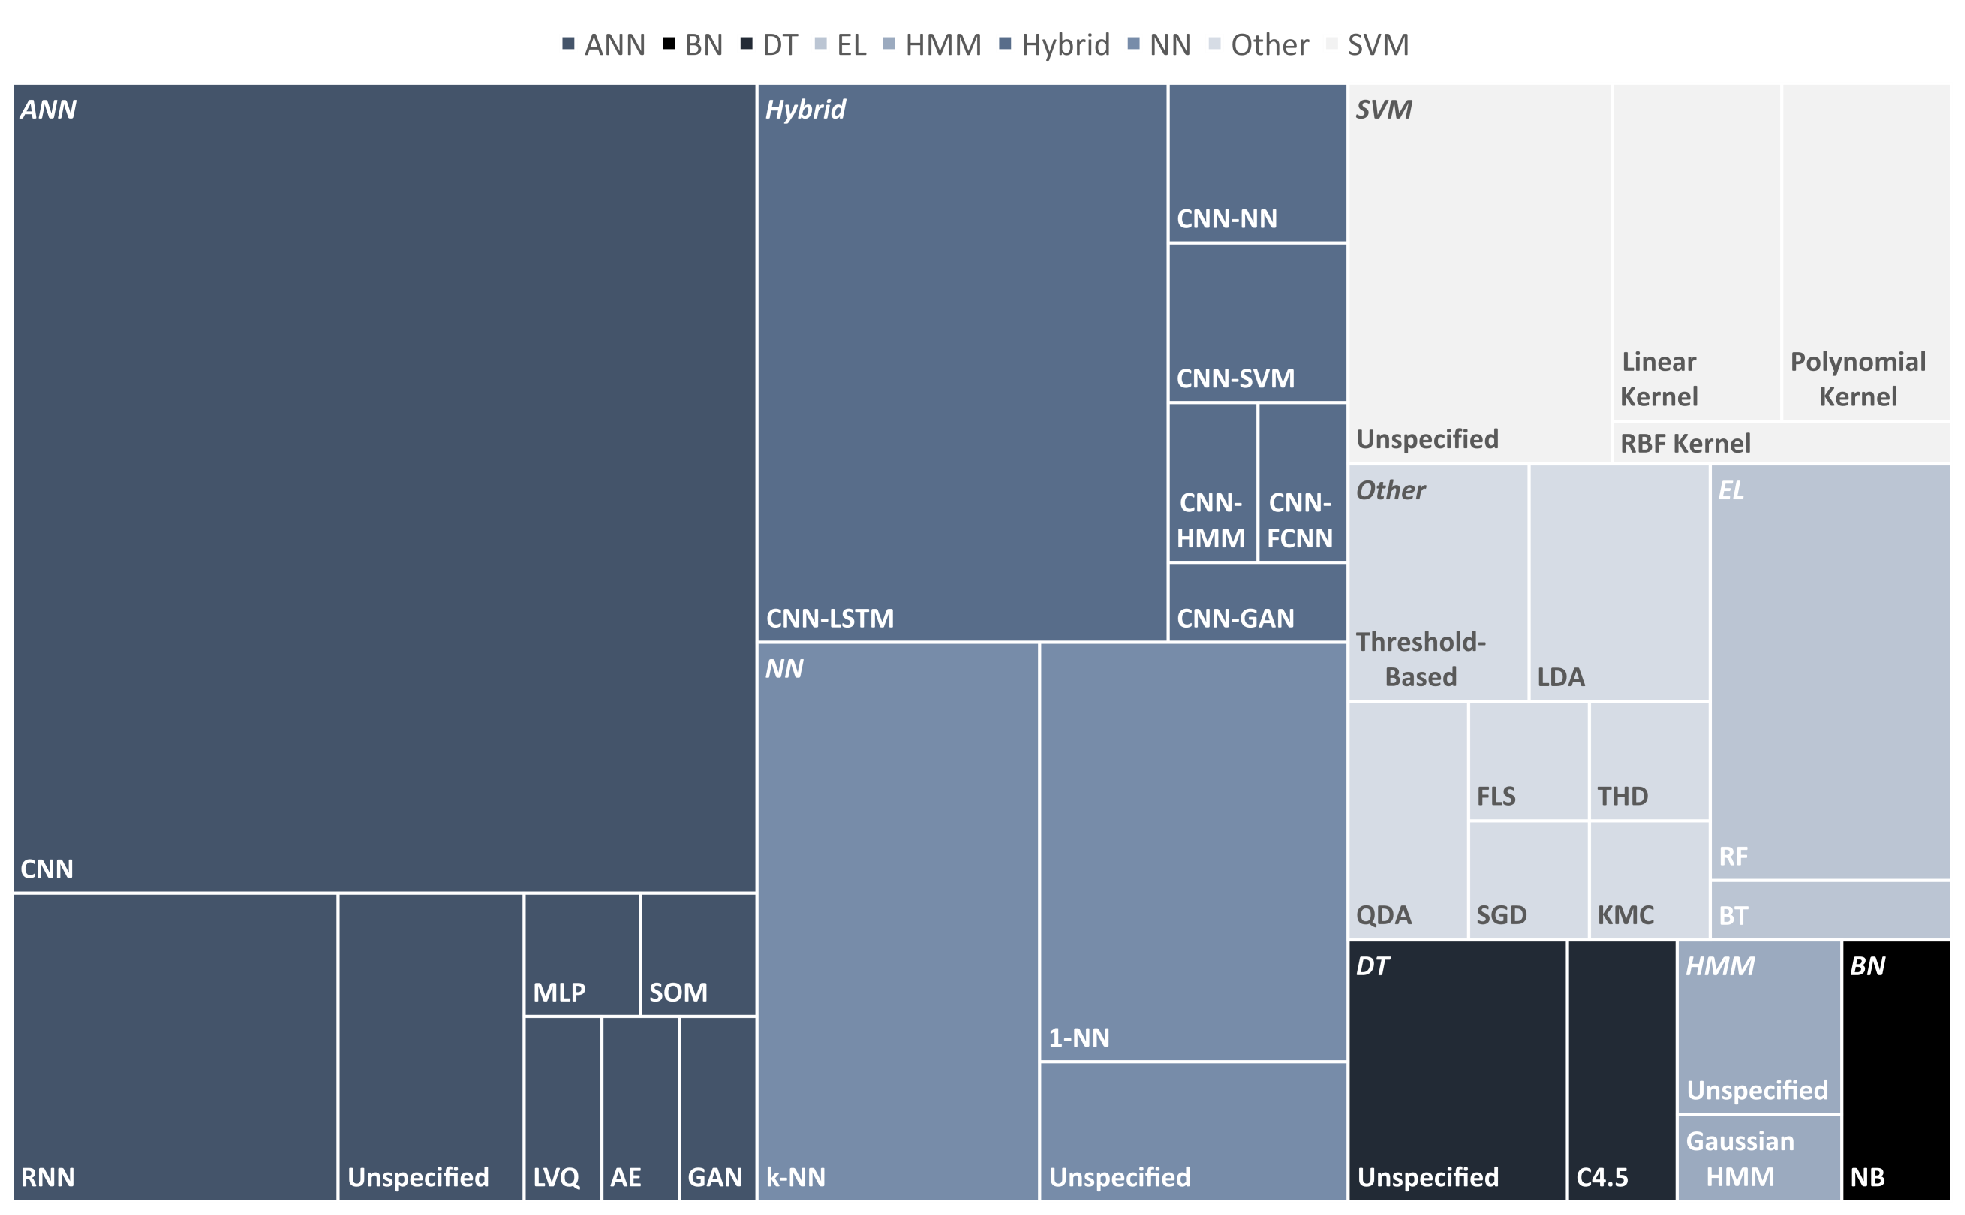
\includegraphics[width=\linewidth]{Figures/StateOfTheArt/Radar/treemap-algorithms.pdf}
    \vspace{-10pt}
    \caption{Tree map~\cite{Shneiderman:1992} of the algorithms for radar-based gesture recognition identified in the corpus. The color of a cell indicates the type of algorithm (\eg ANN, HMM, or SVM) while the size of a cell is proportional to the number of papers featuring this algorithm.}
    \label{fig:state_of_the_art:radar:algorithms}
%    \vspace{-6pt}
\end{figure}


From the above analysis, we make the following observations
\begin{enumerate}
    \item \textit{Predominance of CNN algorithms}: CNNs, often combined with another model like LSTM, are predominant for recognizing radar-based signals. They are particularly appropriate for image processing, but also they benefit from their intrinsic capability to select the discriminant radar features without any human supervision, in particular when dealing with gesture sets that are very large in size and complexity (radar images are very challenging to discriminate by a non-expert).
    %
    \textbf{TODO - Emphasize that the use of point clouds does not require convolutional layers and discuss the impact} 
    It is important to note that CNNs are not the only solution. Instead of relying on CNNs for feature selection, point clouds can be extracted from raw radar signal and directly fed to other algorithms (\eg an LSTM) for gesture recognition\cite{Palipana:2021}. Advantages: \textbf{TODO}
    \item \textit{Dependence of CNN with respect to the radar}: since CNNs automatically select features directly from radar images, these key features are not pre-trained and only learned when the gesture set is examined, thereby making the CNN very appropriate, but also very specific to the radar images produced. The CNNs therefore suffer from a high dependence on radar type and possibly radar unit for a given model. 
    \item \textit{No modeling of the radar functioning}: since CNNs ensure most of the work for a specific radar, we did not identify any work in gesture recognition aimed at modeling the radar functioning in some way to ensure some radar independence or some mechanism to reason about its processing. 
\end{enumerate}



%--------------------------------------------------------------------------------%
\subsection{Gestures} \label{sec:state_of_the_art:radar:gestures}

\begin{figure}[hbt]
    \centering
    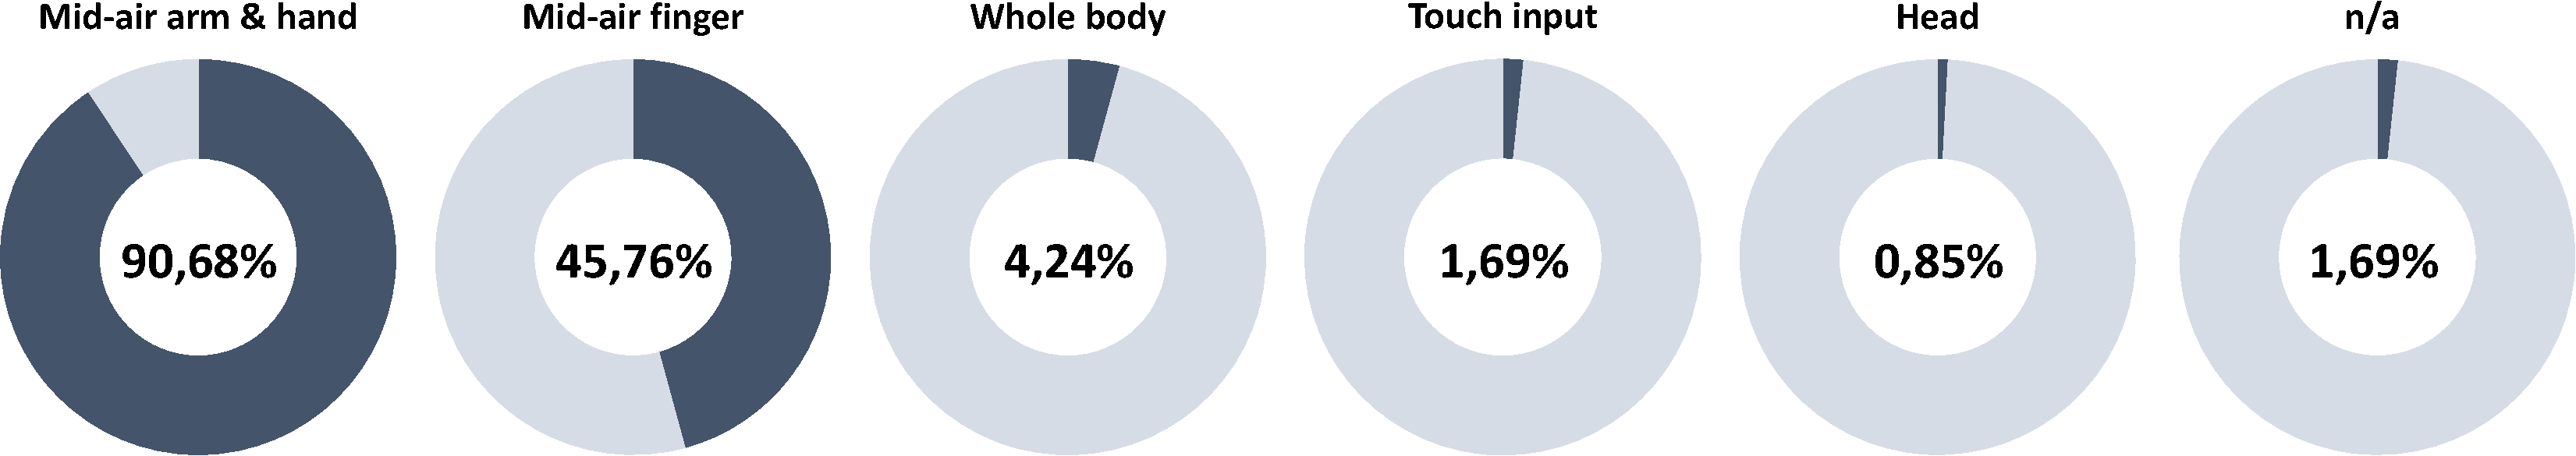
\includegraphics[width=\linewidth]{Figures/StateOfTheArt/Radar/gestures-type.pdf}
    % \vspace{-10pt}
    \caption{Types of gestures.}
    \label{fig:state_of_the_art:radar:gestures-type}
%    \vspace{-6pt}
\end{figure}


\begin{table}[hbt]
    \centering
    %\vspace{-8pt}
    \footnotesize
    \begin{tabular}{>{\raggedright}p{1.8cm}rrr>{\raggedright}p{2.6cm}>{\raggedright}p{0.8cm}>{\raggedright\arraybackslash}p{0.9cm}}
        \toprule
        \textbf{Name} & \textbf{Classes} & \textbf{Users} & \textbf{Samples} & \textbf{Sensor(s)} & \textbf{Base paper} & \textbf{Other papers} \\
        \midrule
        mHomeGes & 10 & 25 & $>$22000 & TI IWR1443 & \cite{Liu:2020b} & /  \\
        \addlinespace[2pt]
        mmASL (wake-words) & 2 & 3 & 3700 & NI multi-FPGA platform (w/ NI PXIe7902, 7976, 3610/3630) and SiBeam phased antenna array & \cite{Santhalingam:2020b} & /  \\
        \addlinespace[2pt]
        mmASL (signs) & 50 & 15 & 12236 & NI multi-FPGA platform (w/ NI PXIe7902, 7976, 3610/3630) and SiBeam phased antenna array + Kinect + RGB camera  & \cite{Santhalingam:2020b} & /  \\
        \addlinespace[2pt]
        deep-soli & 11 & 11 & 5500 & Google Soli & \cite{Wang:2016} & \cite{Berenguer:2019}  \\
        \addlinespace[2pt]
        dop-net & 4 & 6 & 3052 & Ancortek SDR-KIT 2400AD2 & \cite{Ritchie:2020} & \cite{Bannon:2020}  \\
        \addlinespace[2pt]
        HARrad\newline(gestures) & 6 & 9 & 2347 & 77GHz FMCW radar & \cite{Vandersmissen:2020} & /  \\
        \addlinespace[2pt]
        HARrad (events) & 6 & 9 & 1505 & 77GHz FMCW radar & \cite{Vandersmissen:2020} & /  \\
        \bottomrule
    \end{tabular}
    \caption{Summary of the publicly available datasets identified in our systematic literature review.}
    \label{tab:state_of_the_art:radar-slr-datasets}
%   \vspace{-14pt}
\end{table}


\fig~\ref{fig:state_of_the_art:radar:gestures-type} gives an overview of the types of gestures used in the identified papers. Most papers ($\frac{107}{118}=91\%$) featured mid-air arm and hand gestures, which are relatively easy to recognize thanks to their scale that is neither too small, thus not requiring extremely fine range resolution, nor too large, which makes it possible for the radar to focus exclusively on the current user, thus simplifying signal processing. Almost half of the papers ($\frac{54}{118}=46\%$) featured mid-air finger gestures, which require higher frequency radars (capable of finer range resolution) to accurately capture the fine-grained finger motion. Other papers featured whole body gestures~\cite{Li:2009,Li:2020b,Vandersmissen:2020}, touch input~\cite{Copic:2019,Wu:2020}, or even head gestures~\cite{Wan:2014}.
%
We identified only seven publicly available datasets out of the 118 papers from our SLR; see \tab~\ref{tab:state_of_the_art:radar-slr-datasets}. 
The mHomeGes dataset~\cite{Liu:2020b} comprises 10 types of arm gestures collected from 25 participants: arm up/down, push, pull, draw a circle, draw a zigzag, clap hands, mimic knocking on a table, yawn, and lift both arms. Each gesture was recorded in seven environments, including a bedroom and a parlor.
\cite{Santhalingam:2020b} collected 50 different ASL signs from 15 participants in three environments (classroom, laboratory, and conference room) and five different scenarios for single and multiple users. Data were recorded simultaneously with a radar, a Kinect, and an RGB camera.
%
Deep-soli is a dataset introduced by \cite{Wang:2016} that comprises 11 hand gestures performed by 10 users above Google Soli: pinch index/pinky, finger slide, finger rub, slow/fast swipe, push, pull, palm tilt, circle, and palm hold. Deep-Soli was also used by \cite{Berenguer:2019} to evaluate GestureVLAD, their proposed framework for radar gesture recognition.
%
\cite{Ritchie:2020} introduce Dop-net, a dataset of four gestures recorded with two different radar sensors (CW and FMCW). Only the FMCW dataset was released in the form of a challenge. Dop-net was used in another paper to compare the performance of CW and FMCW radars for gesture recognition~\cite{Bannon:2020}.
%
Finally, HARrad consists of two datasets of six gestures of arm and hand gestures collected from nine participants with a 77GHz radar~\cite{Vandersmissen:2020}: drumming, shaking, swiping left/right, and thumb up/down. HARrad events contain six different actions, including entering or leaving a room, sitting down, standing up, clothe, and unclothe.

From the above analysis, we make the following observations:
\begin{enumerate}
\setcounter{enumi}{3}
    \item \textit{Limited availability of datasets}: very little datasets are available for benchmarking.
    \item \textit{Huge size of datasets}: the size of the raw data captured for a single gesture is very high, making the entire dataset huge in size and challenging to process. Little or no dimension reduction has been observed.
\end{enumerate}

%--------------------------------------------------------------------------------%
\subsection{Radars} \label{sec:state_of_the_art:radar:sensors}

We identified 123 radar systems and extracted their parameters, including the radar type, the frequency band in which they operate, the model, and their position. We identified four types of radars (\fig~\ref{fig:state_of_the_art:radar:types}): 
\begin{itemize}
    \item \textit{Frequency-Modulated Continuous-Wave} (FMCW) radars ($\frac{65}{123}{=}53\%$), which continuously transmit a signal that varies in frequency, \ie modulated in frequency. These radars can resolve both the range and Doppler~\cite{AlHourani:2018}, enabling the recognition of static poses and dynamic gestures.
    
    \item \textit{Unmodulated Continuous-Wave} (CW) radars ($\frac{36}{123}{=}29\%$), which continuously transmit a signal at a constant frequency and amplitude~\cite{Oberhammer:2013}. These radars are simple and inexpensive. They can measure the Doppler shift of the return signal caused by moving objects but cannot provide range information or identify stationary targets, as the latter do not cause a Doppler shift. Consequently, radars of this type are not suitable for detecting static poses of the hand or body.
    
    \item \textit{Pulse} radars ($\frac{21}{123}{=}17\%$) transmit short radar pulses and listen for the returning echo. These radars can measure the range of targets, stationary and moving, making them suitable for the recognition of static poses and dynamic gestures. The pulse length affects the radar detection range (a longer pulse length increases the maximum range but may prevent the detection of very close targets) as well as its range resolution (a shorter pulse length allows for better discrimination between two spatially separated targets)~\cite{Bole:2014}. The smaller the pulse length in the time domain, the larger the bandwidth in the frequency domain counterpart.
    
    \item  \textit{Direct-Sequence Spread Spectrum} (DSSS) radars ($\frac{1}{123}{=}1\%$)  transmit signals modulated by a random bit sequence. These radars can measure the range of stationary and moving targets, and their architecture is simpler than FMCW radars~\cite{Tang:2020}.
\end{itemize}

\begin{figure}[t]
    \begin{subfigure}{.49\textwidth}
        \centering
        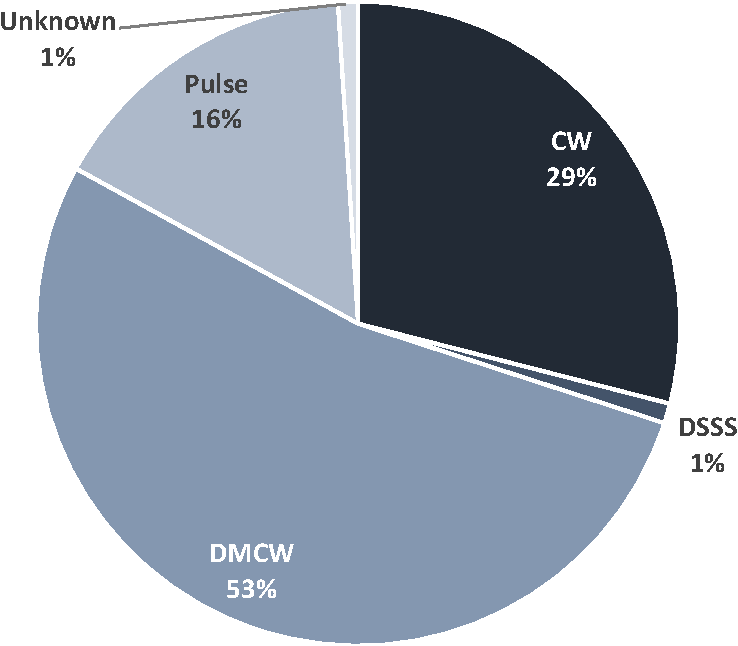
\includegraphics[height=.75\linewidth]{Figures/StateOfTheArt/Radar/radar-types.pdf}
        % \vspace{-6pt}
        \captionsetup{width=.9\linewidth}
        \caption{Radar type.}
        \label{fig:state_of_the_art:radar:types}
    \end{subfigure}
    \begin{subfigure}{.49\textwidth}
        \centering
        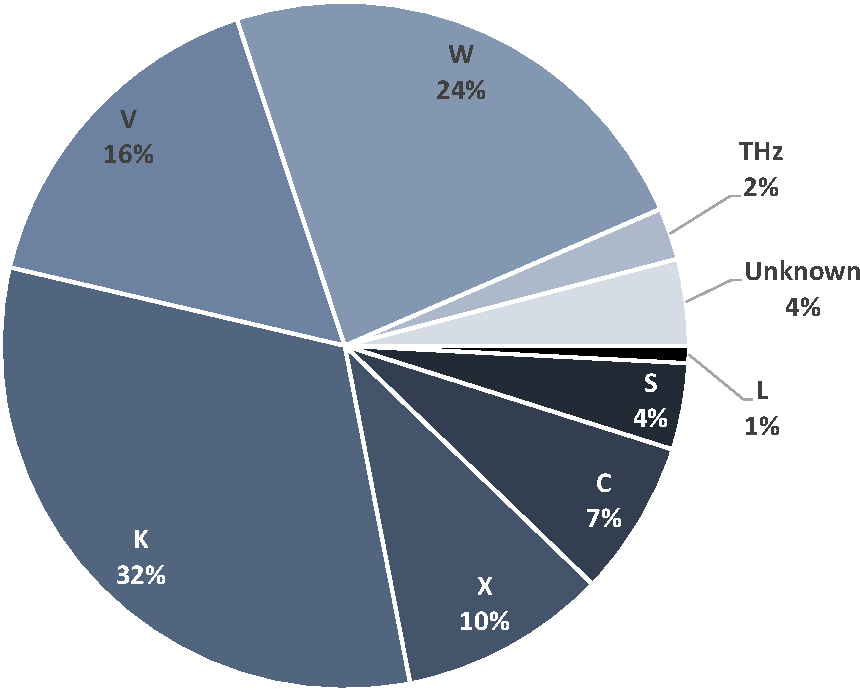
\includegraphics[height=.75\linewidth]{Figures/StateOfTheArt/Radar/radar-frequencies.pdf}  
        % \vspace{-6pt}
        \captionsetup{width=.9\linewidth}
        \caption{Frequency band~\cite{IEEE:2020}.}
        \label{fig:state_of_the_art:radar:frequencies}
    \end{subfigure}
    \caption{Distribution of the radars identified in our systematic literature review.}
    \label{fig:state_of_the_art:radar:pie-charts}
    % \vspace{-8pt}
\end{figure}
%The type of one radar ($\frac{1}{123}{=}1\%$) could not be identified. 
Most of the papers ($\frac{98}{118}{=}83\%$) relied on a single radar sensor to capture gestures, while the rest ($\frac{20}{118}{=}17\%$) used two or more radars. Among the latter, four papers introduced different radar models. Some papers introduced other types of sensors, such as~\cite{Santhalingam:2020b}, where gestures were collected using a radar, a Kinect, and an RGB camera for comparison purposes. \cite{Gigie:2019} synthesized micro-Doppler radar signatures of gestures from the skeleton provided by a Kinect. Other papers performed data fusion with RGB cameras~\cite{Molchanov:2015,Vandersmissen:2020}, depth cameras~\cite{Tzadok:2020,Molchanov:2015}, and thermal cameras~\cite{Skaria:2020b}, respectively.

\fig~\ref{fig:state_of_the_art:radar:radar-position} summarizes the position of the radar systems identified in the user environment. Almost half of the identified papers ($\frac{49}{118} = 42\%$) did not provide enough information about the position of the radar(s) in the user's environment. From the papers that provided this information, 47 ($\frac{47}{118} = 40\%$) placed the radar(s) on a table, while 10 ($\frac{10}{118} = 8\%$) placed them on a tripod, and six ($\frac{6}{118} = 5\%$) in the car (\eg on the center console~\cite{Molchanov:2015}, near the steering wheel~\cite{Ahmed:2019, Sun:2018}, or on the roof console~\cite{Sun:2019}). Other positions include on the body~\cite{Miller:2020,Copic:2019}, on fabric~\cite{Wu:2020}, and on a robot~\cite{Li:2009}.

\begin{figure}[t]
    \centering
    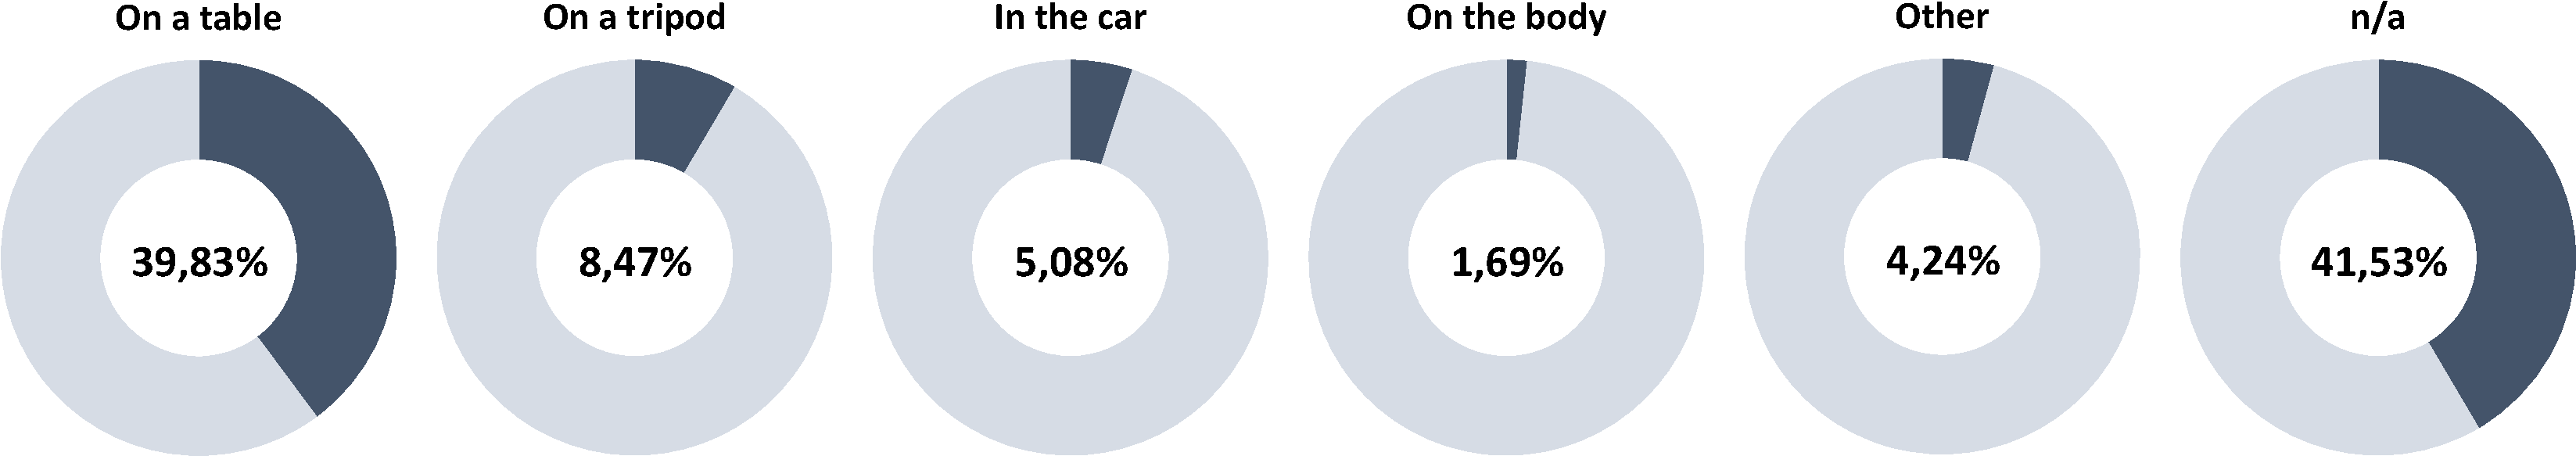
\includegraphics[width=\linewidth]{Figures/StateOfTheArt/Radar/radar-positions.pdf}
    % \vspace{-10pt}
    \caption{Positions of the radar.}
    \label{fig:state_of_the_art:radar:radar-position}
%    \vspace{-6pt}
\end{figure}

\begin{figure}[t]
    \centering
    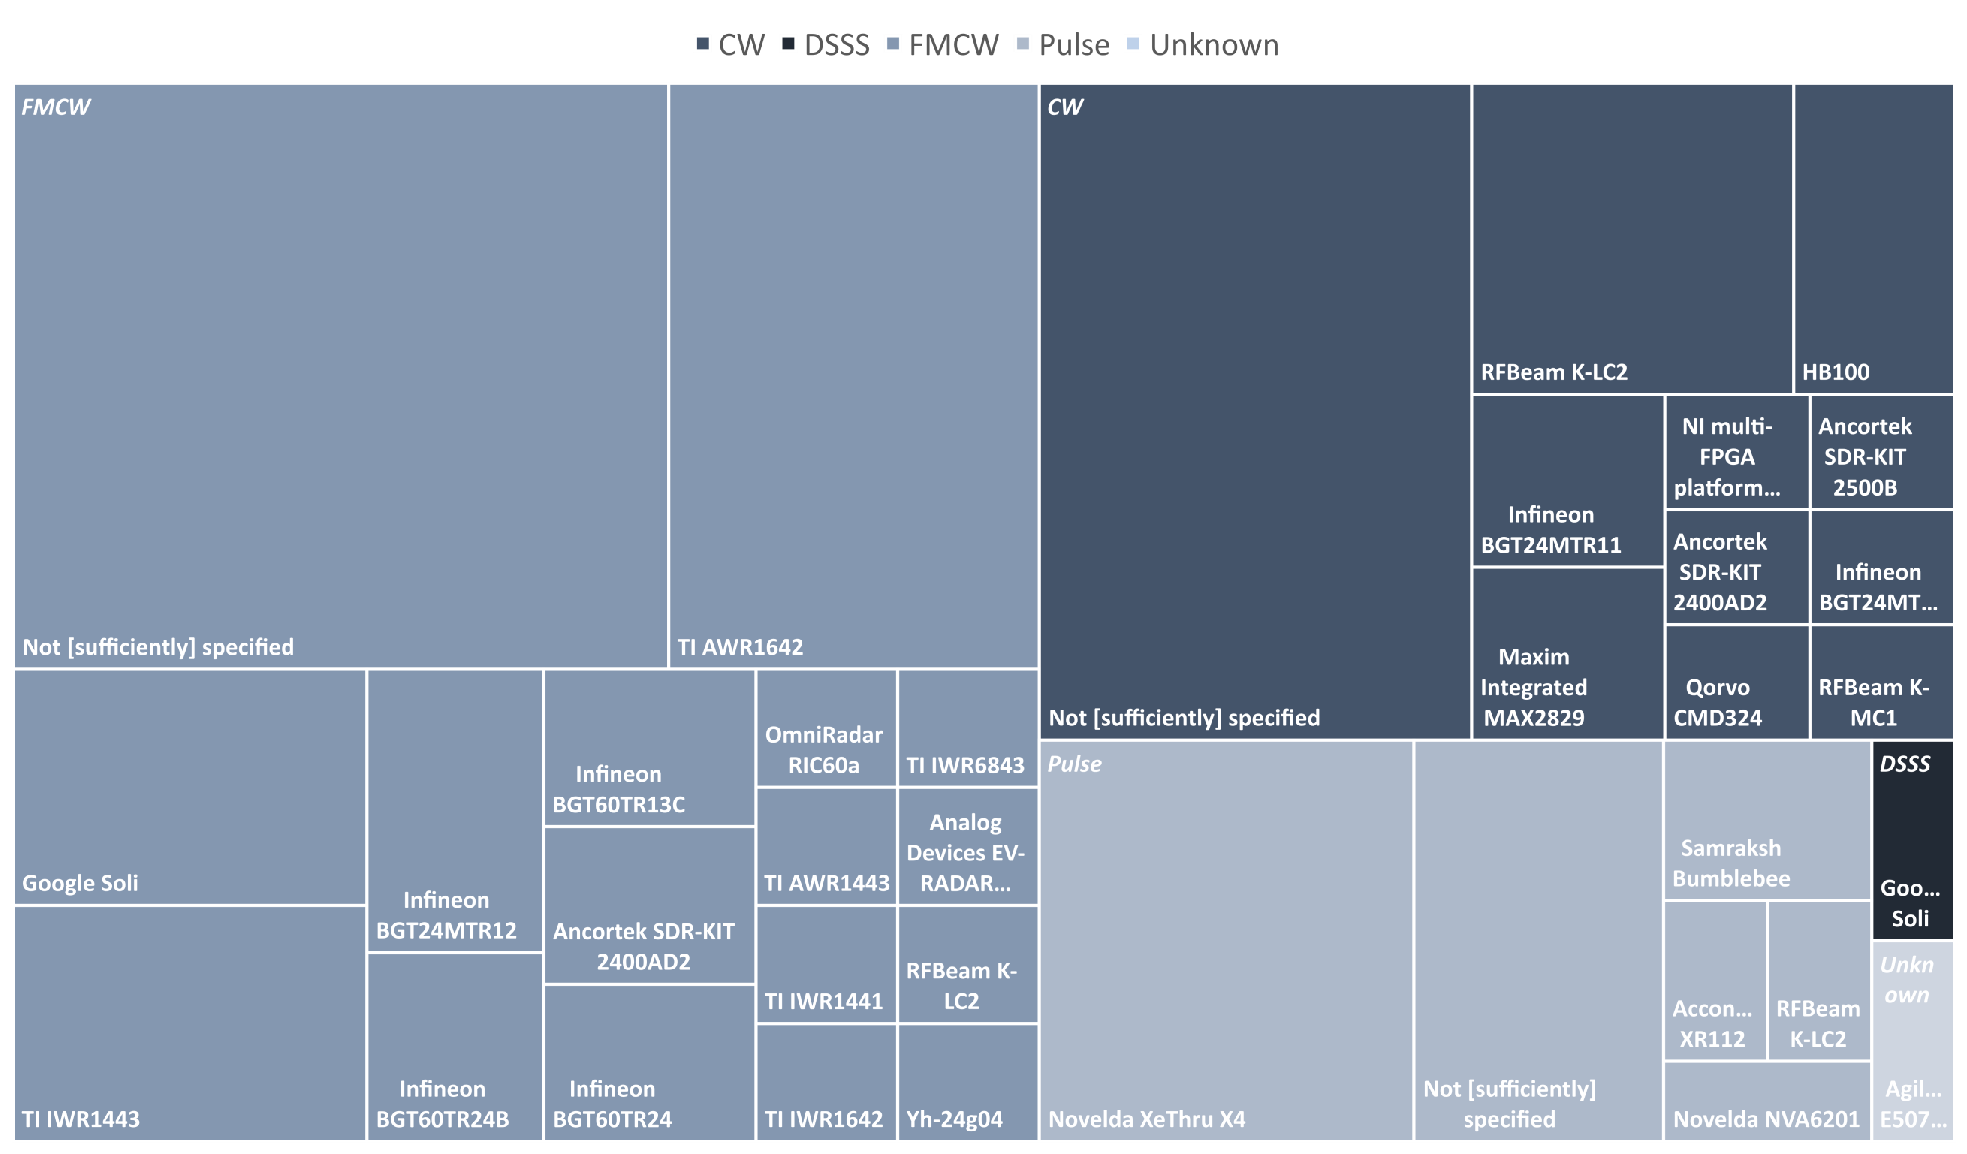
\includegraphics[width=\linewidth]{Figures/StateOfTheArt/Radar/treemap-radar-types-models.pdf}
    \vspace{-16pt}
    \caption{Tree map~\cite{Shneiderman:1992} of the radar models identified in our systematic literature review. 
    The color of a cell indicates the type of radar (CW, DSSS, FMCW, Pulse, or unknown) while the size of a cell is proportional to the number of papers featuring this model of radar.}
    \label{fig:state_of_the_art:radar:radars}
    %\vspace{-8pt}
\end{figure}

\begin{figure}[t]
    \centering
    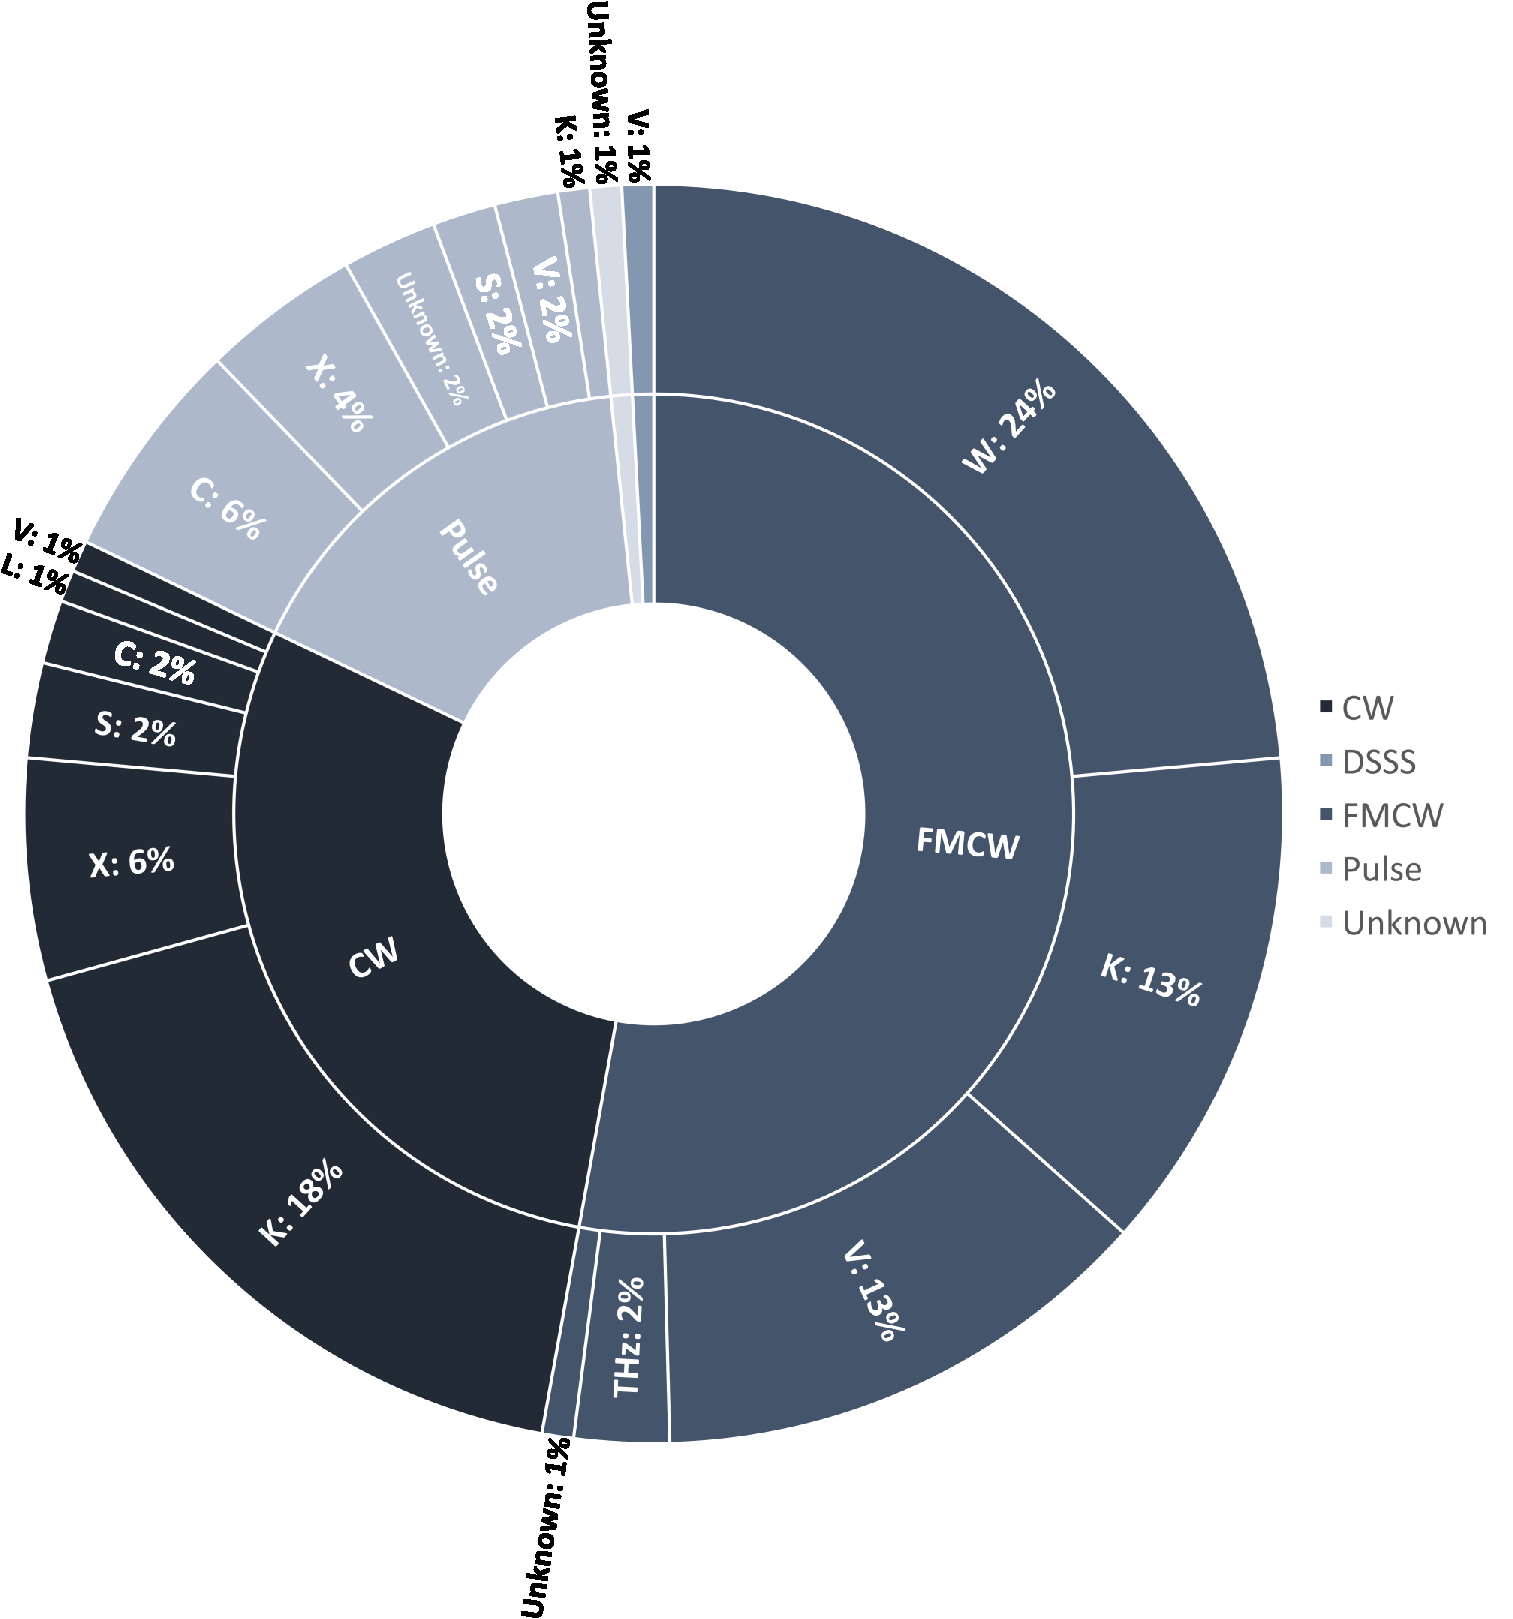
\includegraphics[width=.6\linewidth]{Figures/StateOfTheArt/Radar/diagram-radar-types-frequencies.pdf}
    \vspace{-4pt}
    \caption{Sunburst chart of the radars identified in the SLR. The inner ring and color show the proportion of each radar type, while the outer ring indicates the proportion of each frequency band for each radar type according to the IEEE standard~\cite{IEEE:2020}.}
    \label{fig:state_of_the_art:radar:radars-types-frequencies}
    \vspace{-4pt}
\end{figure}

We also classified radars according to their frequency band according to the IEEE Standard Letter Designations for Radar-Frequency Bands~\cite{IEEE:2020} (\fig~\ref{fig:state_of_the_art:radar:frequencies}). The larger the frequency band, the better resolution the radar provides, and, in principle, the finer the gestures can be acquired. \fig~\ref{fig:state_of_the_art:radar:frequencies} shows that most of the radars ($\frac{88}{123} = 72\%$) operate in the K (18 to 27 GHz, 32\%), V (40 to 75 GHz, 16\%), and W (75 to 110 GHz, 24\%) bands. The V-band encompasses the Google Soli~\cite{Lien:2016}, which operates at 60 GHz and was used in five papers~\cite{Lien:2016,Wang:2016,Copic:2019,Berenguer:2019,Choi:2019} identified by our SLR. Three papers used very high-frequency THz-band radars (300 to 1000 GHz) to achieve better resolution~\cite{Wang:2019b,Wang:2020b,Zhou:2018a}. Only $\frac{27}{123}=22\%$ of the radars operated at frequencies below 18 GHz:
10\% in the X-band (8 to 12 GHz),
7\% in the C-band (4 to 8 GHz),
4\% in the S-band (2 to 4 GHz),
and 1\% in the L-band (1 to 2 GHz). The benefit of lower frequencies is the larger detection range. For a given application, a trade-off has therefore to be chosen between resolution and range. The detection range can also be increased by increasing the transmitted power, but this increases energy consumption and can lead to adverse health effects. 
\fig~\ref{fig:state_of_the_art:radar:radars-types-frequencies} summarizes the distribution of frequency bands by radar type.

Finally, we extracted the radar models used in the papers that provided this information; see \fig~\ref{fig:state_of_the_art:radar:radars}. % shows a wide variety of radar models with a tree map visualization~\cite{Shneiderman:1992}. 
More than a third of the papers ($\frac{46}{123} = 37\%$) did not provide enough information to identify the exact models. Of the 77 remaining publications, we identified 29 unique models %, which depict a rather fragmented landscape. 
with the most popular being the Texas Instruments AWR1642 ($\frac{13}{123} = 11\%$) and IWR1443 ($\frac{5}{123} = 4\%$), the Novelda XeThru X4 ($\frac{9}{123} = 7\%$), the RFBeam K-LC2 ($\frac{8}{123} = 7\%$), and Google Soli ($\frac{6}{123} = 5\%$), respectively. Except for Google Soli, which was designed for integration into smartphones and smart speakers, most of the radar systems from the SLR were not meant for everyday use. However, some of the papers introduce prototypes of radars that could be integrated into furniture~\cite{Mcintosh:2017} or even stitched into clothing~\cite{Wu:2020}.

From the above analysis, we make the following observations:
\begin{enumerate}
\setcounter{enumi}{5}
    \item \textit{Predominance of FMCW over other types of radar (\fig~\ref{fig:state_of_the_art:radar:types} and~\ref{fig:state_of_the_art:radar:radars-types-frequencies})}: these radars are the most frequently exploited due to their ability to sense both static and dynamic gestures but also because several models are commercially available. The frequency bands covered by these two categories are high enough to acquire raw data with high resolution.
    \item \textit{Limited coverage of very low/high-frequency bands} (\fig~\ref{fig:state_of_the_art:IEEE}): lower frequencies result in worse range resolution, making it more difficult for the radar to distinguish between two targets. Such radars are thus less interesting for smaller-scale gestures, such as hand and finger gestures, which explains the lower number of works covering these systems. On the contrary, higher frequencies enable better range resolution and thus are better suited for small-scale hand and finger gestures (\eg Google Soli~\cite{Lien:2016,Wang:2016}), at the cost of higher complexity and lower range as the frequency increases. Most systems operate at frequencies between 4 GHz and 100 GHz, which can provide sufficient range resolution with relatively low complexity and power consumption. In addition, some off-the-shelf radar systems used in HCI research were originally developed for other applications and operate specific frequencies, such as collision avoidance systems in cars, which often operate in the K-band. 
\end{enumerate}

\begin{figure}[t]
    \centering
    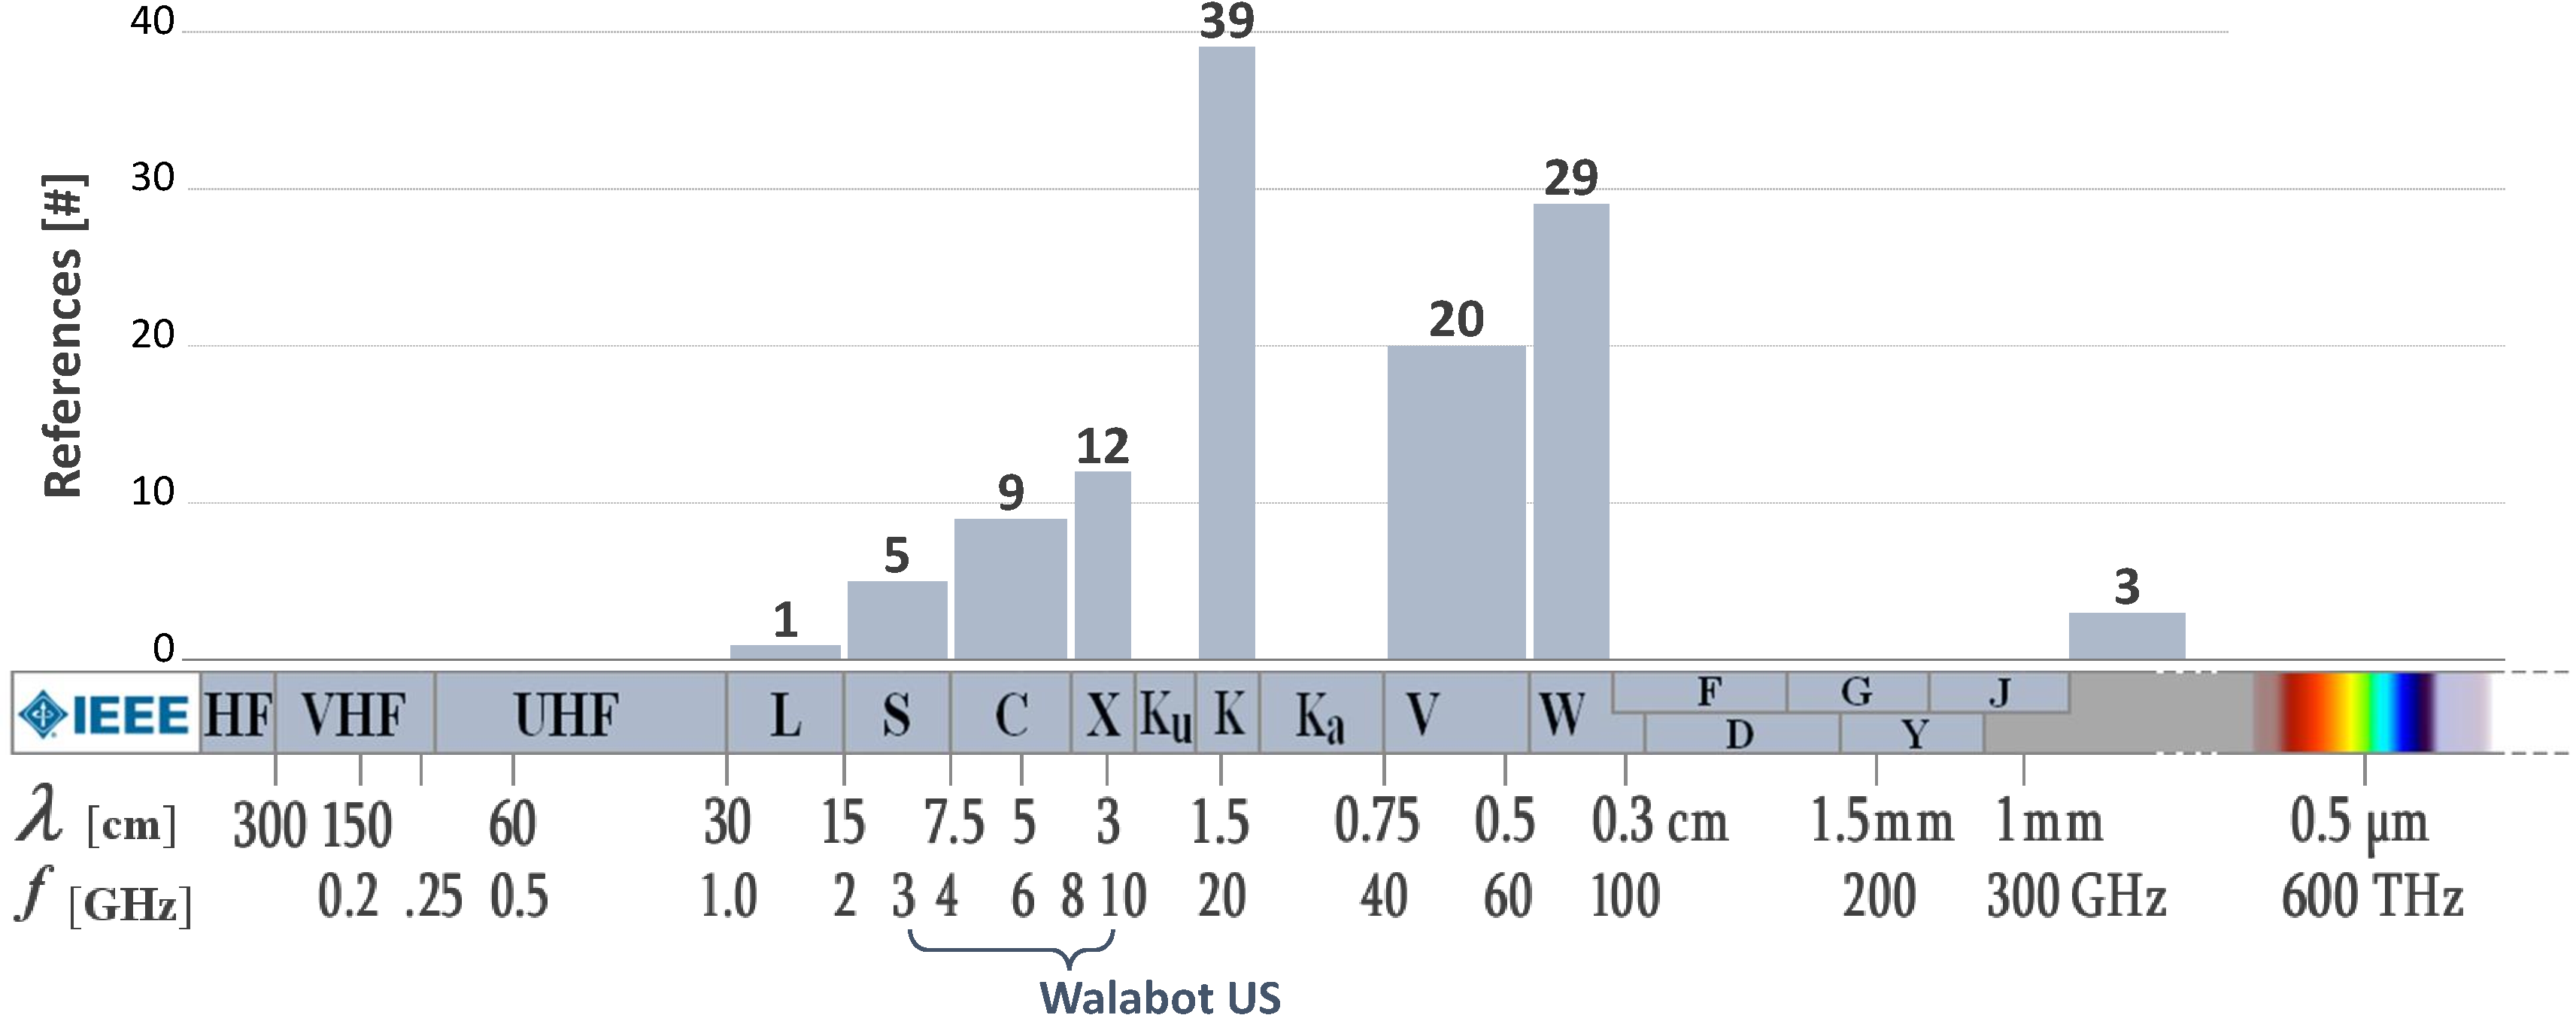
\includegraphics[width=\textwidth]{Figures/StateOfTheArt/Radar/IEEE-bands.pdf}
    \vspace{-12pt}
    \caption{Number of radar systems according to their frequency band~\cite{IEEE:2020} distributed along the electromagnetic continuum (Bottom image of waves and frequency ranges used by radar used with permission from Christian Wolff~\cite{Wolff:2022}), from a total of 118 radars. Five radars did not mention their frequency band.}
    \label{fig:state_of_the_art:IEEE}
    \vspace{10pt}
\end{figure}

%--------------------------------------------------------------------------------%
\subsection{Summary} \label{sec:state_of_the_art:radar:summary}
Radar-based gesture recognition is still in its infancy. Current research mostly focuses on radar systems, signal processing, and algorithms for gesture recognition. As a result, few papers demonstrate a potential use case of their system with a prototype application.
%
In addition, most of the papers rely on deep learning techniques tailored to a specific radar system and gesture set. The combination of a wide variety of sensors, often custom-designed, and a lack of publicly available datasets makes it difficult to reproduce and compare results.

%================================================================================%
\section{Positioning this Work in the Literature} \label{sec:state_of_the_art:this_work}
This chapter provided an overview of gesture-based interaction in the literature. We looked at how to involve users in the development process of gesture-based applications through GESs and identified the main challenges faced by developers when implementing real-time gesture recognition. These challenges include taking into account sensor limitations, extracting gestures from a continuous flow of data, and supporting some variability in the gestures produced by end users.
%
We then had an in-depth look at the LMC, an affordable off-the-shelf device for vision-based gesture recognition. Despite the popularity of this device, most of the papers identified implemented gesture recognition in an opportunistic manner, which could not be adapted easily to support other devices, gestures, or applications. This highlights a need for a tool that would enable the efficient reuse of components designed by, \eg the scientific community, in the development of gesture-based applications.
%
We made several observations regarding three of the four software quality properties defined in Section~\ref{sec:introduction:research:research-questions}.
%
Regarding \textit{maintainability}, we observed a reliance of many papers on non-reusable, often opportunistic, approaches to gesture recognition. As such, supporting other gestures may be impossible without completely re-writing the gesture recognition logic. In addition, we noticed a lack of clear separation of concerns between user interfaces and their gesture recognition logic, which often unnecessarily complicates future modifications.
%
Similarly, the reliance on these opportunistic approaches hinders software \textit{portability}, as they are often tied to the exact sensor used. Supporting other sensors would thus require substantial work. 
%
As for \textit{usability}, the scarcity of tools available to developers presents significant entry barriers for creating highly usable gesture-based applications. Indeed, developing such applications currently requires expertise in gesture recognition, UX design, and application development.

We also looked at radar-based gesture recognition, to identify any application, algorithm, sensor, and dataset described in the literature. 
%
Regarding the \textit{compatibility} software quality property, we observed a scarcity of publicly available datasets and noted that most gesture recognition techniques were tailored for one radar system in particular, making it difficult to reuse datasets across different systems.
%
From a \textit{maintainability} point of view, a majority of the analyzed papers relied on deep learning techniques for gesture recognition. While effective, they posed a challenge for future updates, as changing the sensor or the gesture set could require extensive re-training to achieve the same level of performance.
%
In terms of \textit{portability}, we did not observe any consensus on an affordable and efficient off-the-shelf radar sensor, resulting in a plethora of different (custom) radar systems. Making matters worse, a large part of the proposed gesture recognition techniques were specific to one sensor and gesture set, which limited their applicability to other applications.
%
Regarding \textit{usability}, we noticed that very few papers demonstrated potential use cases of their system with prototype applications. In addition, most of the proposed techniques could not support user-submitted gestures without extensive re-training, which could negatively impact usability, should they be used in real applications~\cite{Nacenta:2013}.

In conclusion, most of the papers that we analyzed in this chapter did not properly address four of the ISO/IEC 25010 software quality properties~\cite{iso25010}, namely compatibility, maintainability, portability, and usability. 
%
Having identified the main challenges of (radar-based) gesture recognition, the rest of this thesis will focus on the development of tools and methods that streamline the development of highly usable gesture interfaces.






\chapter{Facilitating the Development of Gesture-based Applications} \label{chap:quantumleap}

The landscape of contactless UIs is constantly evolving. Sensors such as the LMC are paving the way towards cheap and accurate gesture recognition, while researchers are continuously working on improving gesture recognition algorithms.
However, the lack of a common framework for gesture recognition is making it increasingly harder to keep track of this evolution outside of the research community, resulting in only a handful of real-life applications (see Sections~\ref{sec:state_of_the_art:overview:applications} and \ref{sec:state_of_the_art:lmc}). 
%
As such, this chapter attempts to answer two of the five research questions defined in Section~\ref{sec:introduction:research:research-questions}: 
\begin{itemize}
    \item [RQ4] \textit{How can we foster collaboration between researchers and practitioners working on (radar) gesture recognition?} 
    \item [RQ5] \textit{How can tools and methods aid in designing gesture-based applications that operate independently of gesture recognition logic?}
\end{itemize}
To that end, it introduces \ql, a software tool that aims at bridging the gap between researchers and developers by providing a common framework to (1) help researchers share the results of their work in a way that is easily reusable and (2) allow developers to create gesture-based applications without spending time to solve the numerous challenges of gesture recognition (see Section~\ref{sec:state_of_the_art:overview:challenges}). The main contribution of this chapter and how it fits into the rest of this thesis are summarized in \fig~\ref{fig:quantumleap:graphical-summary}.

\begin{figure}
    \centering
    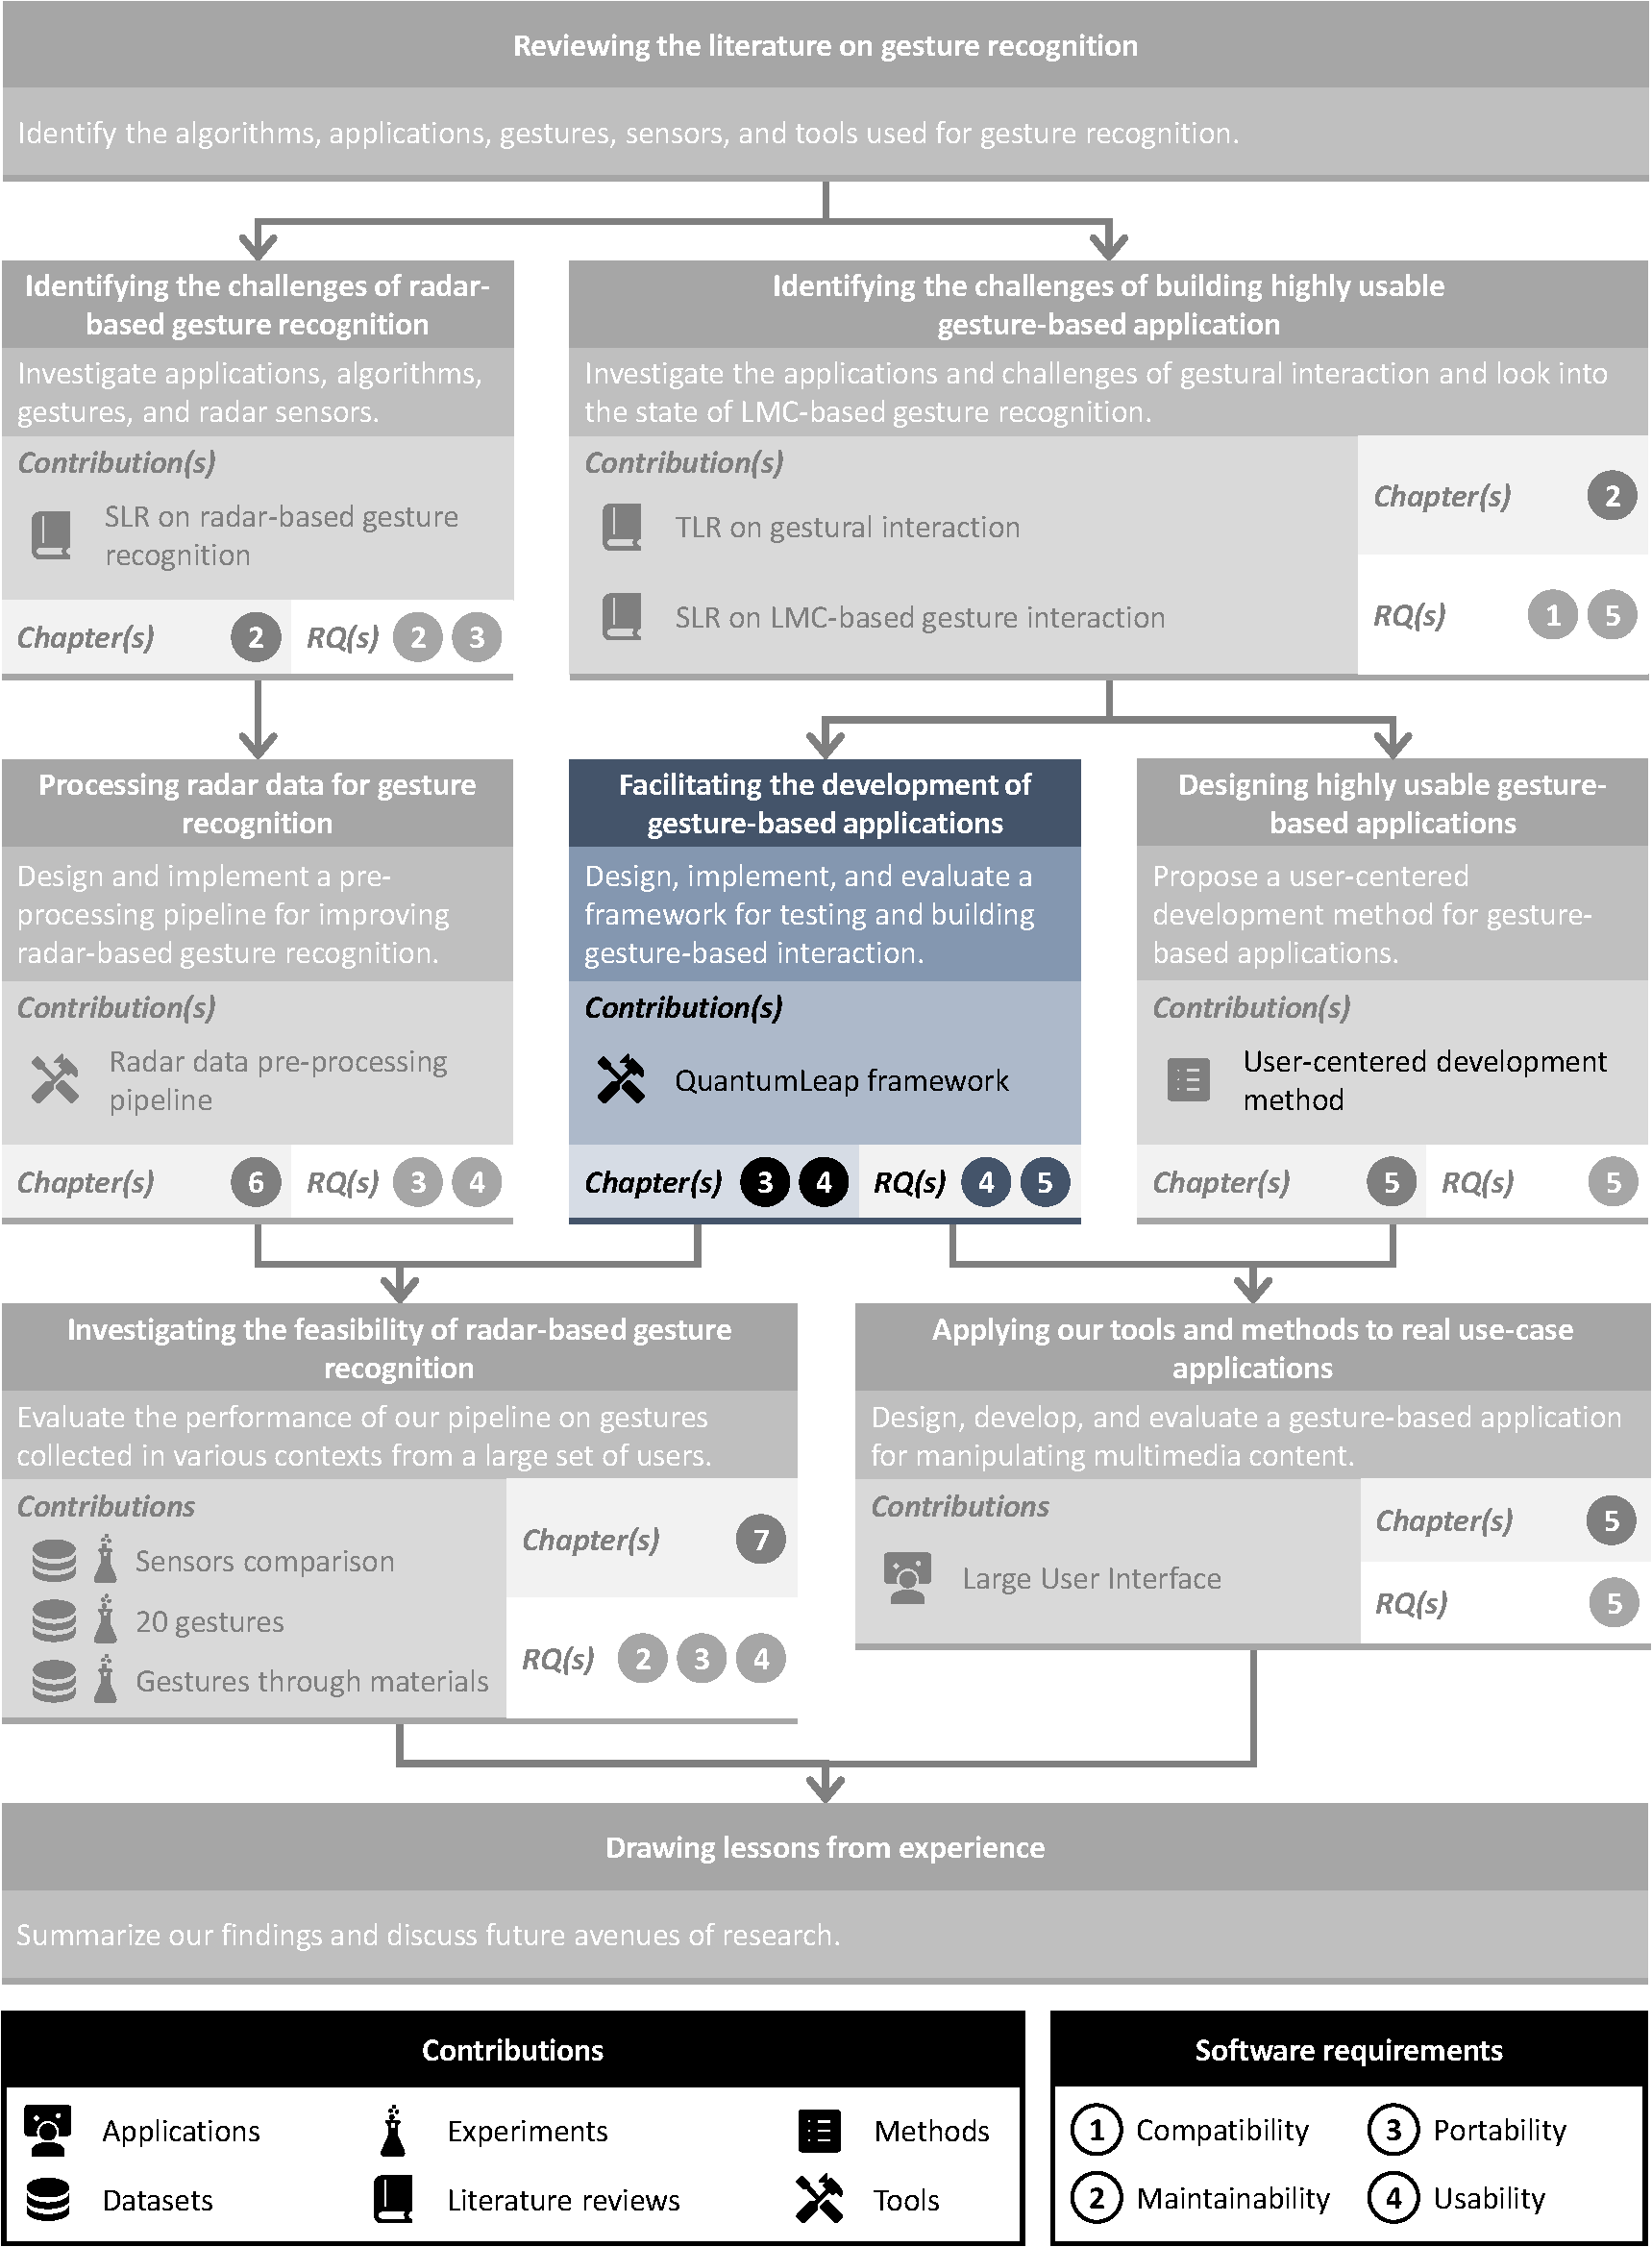
\includegraphics[width=\linewidth]{Figures/QuantumLeap/graphical-summary-quantumleap.pdf}
    \vspace{-18pt}
    \caption{Main contributions of this chapter.}
    \label{fig:quantumleap:graphical-summary}
\end{figure}

The rest of this chapter is organized as follows. Section~\ref{sec:quantumleap:description} first provides an in-depth description of \ql, including its dataflow architecture, configuration, and API.
Section~\ref{sec:quantumleap:evaluation} discusses the results of an experiment aimed at evaluating the overall usability of \ql, which involved seven developers with different levels of expertise.
Section~\ref{sec:quantumleap:integration} then explores how some recent projects utilized and extended the framework.
Finally, Section~\ref{sec:quantumleap:discussion} discusses the advantages and limitations of \ql, and Section~\ref{sec:quantumleap:conclusion} concludes this chapter.

\paragraph{Publications.} This chapter is adapted from a paper published in the EICS 2022 conference proceedings~\cite{Sluyters:2022:EICS}.

\paragraph{Resources.} The \ql framework is available on GitHub at \url{https://github.com/sluyters/QuantumLeap}. Demonstration videos of applications built with \ql are available at \url{https://www.youtube.com/playlist?list=PLj1KcEqIa0fHyDyeW_NpiLHCP6A8j7mS3}.


%================================================================================%
\section{A Framework for Building Gesture-Based Applications} \label{sec:quantumleap:description}

\ql is designed as an intermediate layer between gesture-based applications and gesture sensors. It contains all of the logic necessary for gesture recognition and only exposes a simple JavaScript API that allows developers to map gestures to actions without focusing on acquiring, segmenting, and recognizing gestures. 
Implemented in JavaScript (ECMAScript 2019)~\cite{Ecma:2017}, the \ql framework is divided into two parts according to Pree's notation \cite{Pree:1994}: \textit{frozen spots}, which are ``fixed'' parts which remain constant for all of its instantiations, and \textit{hot spots}, which are generic parts to be modified depending on the context of use~\cite{Calvary:2003}.
\ql is a \textit{gray box} software framework~\cite{Parsons:1999}, as it provides developers with two options: pick modules from a list of predefined components (black box) or write new components that meet their needs better (white box).
The rest of this section describes the overall software architecture of \ql.
%, its API, and how it can be configured for a specific context of use.

%--------------------------------------------------------------------------------%
\subsection{Dataflow Architecture} \label{sec:quantumleap:description:architecture}

The dataflow architecture of \ql (\fig~\ref{fig:quantumleap:archi}) has been designed to be versatile and simple to configure (Section~\ref{sec:quantumleap:description:configuration}). It consists of eight modules (\ie hot spots), each stemming from the challenges of gesture recognition discussed in Section~\ref{sec:state_of_the_art:overview:challenges}: a sensor module, filtering module, loaders for static and dynamic datasets, static and dynamic gesture recognizers, gesture segmentation module, and an analyzer module. Various implementations are provided for each module to suit the needs of a specific application (see Appendix~\ref{app:quantumleap-modules}). When these implementations are not suited for a particular application, the framework is extensible and developers are thus encouraged to propose new implementations. The modules communicate together using various data structures described in \tab~\ref{tbl:quantumleap:communication-data-structures}. 
The rest of this section provides information about each type of module.

\begin{table}[t]
    \footnotesize
    \centering
    \begin{tabular}{lp{10.8cm}}
        \toprule
        \textbf{Id} & \textbf{Description} \\
        \midrule
        1 & \custominlinecode{Frame} object. \\
        2 & \custominlinecode{Sample} object. \\
        3 & JavaScript object with three properties: the gesture type (\ie static or dynamic), the gesture name, and the data from the analyzer if the gesture is static. \\
        4 & WebSocket message of type \custominlinecode{Data} containing frames and static\slash dynamic gestures if detected. \\
        5 & WebSocket message of type \custominlinecode{Operation}. \\
        \bottomrule
    \end{tabular}
    \caption{Data structures for inter-module communication.}
    % \vspace{-18pt}
    \label{tbl:quantumleap:communication-data-structures}
\end{table}



\begin{figure}[t]
    \centering
    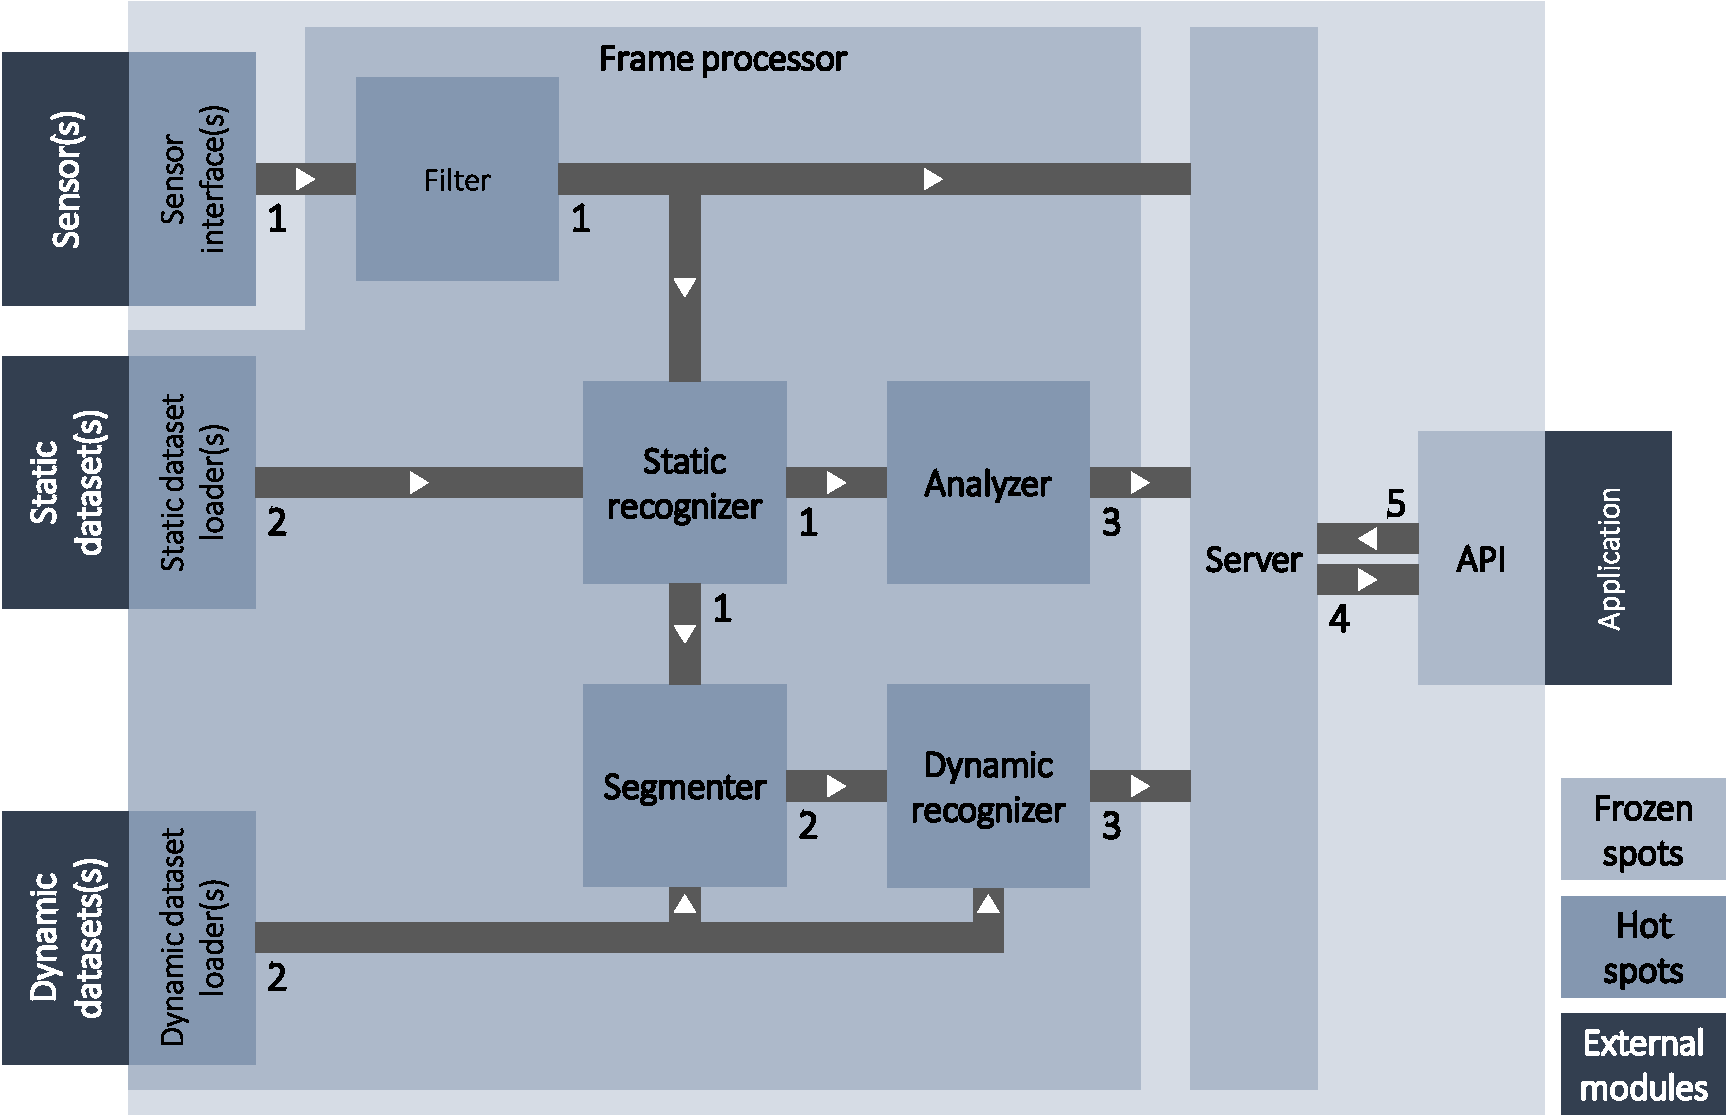
\includegraphics[width=\linewidth]{Figures/QuantumLeap/Architecture/quantumleap.pdf}
    \vspace{-8pt}
    \caption{\ql dataflow architecture.}
    % \vspace{-8pt}
    \label{fig:quantumleap:archi}
\end{figure}

\subsubsection{Sensor} 
This module serves as an interface between \ql and any physical sensor, such as an LMC, a radar sensor, or a Microsoft Kinect. It transforms raw, sensor-specific data into a standardized format usable throughout the framework. This module is called a set number of times per second by \ql to retrieve tracking data at one instant in time. Depending on the context of use, multiple sensor modules may be combined, \eg to increase recognition accuracy. A sensor module should implement three methods:
\begin{itemize}[noitemsep]
    \item \custominlinecode{getPoints(timestamp)}: get a list of points from the sensor at this instant in time.
    \item \custominlinecode{connect()}: connect to the sensor.
    \item \custominlinecode{disconnect()}: disconnect from the sensor.
\end{itemize}
One sensor module is provided with \ql. Its description can be found in Appendix~\ref{app:quantumleap-modules:sensors}.

\subsubsection{Filter}
As discussed in Section~\ref{sec:noise}, noise can negatively impact the user experience by reducing pointing and gesture recognition accuracy. Before it can be used by the other modules, each frame is first processed by the filter module, which computes a new frame with reduced noise. Filtering should be carefully tuned to fit the sensor and the target application, as too much noise reduction runs the risk of introducing some lag. A filter module should implement one method:
\begin{itemize}[noitemsep]
    \item \custominlinecode{filter(frame)}: compute a new frame with less noise.
\end{itemize}
Four different modules are provided and described in Appendix~\ref{app:quantumleap-modules:filters}.

\subsubsection{Static and Dynamic Datasets}
These modules transform a gesture dataset into a \custominlinecode{GestureSet} object, \ie a standardized format compatible with the framework. Datasets are then used to train the static and dynamic recognizers.
\begin{figure*}[p]
    \centering
    % \vspace{-6pt}
    \captionsetup{justification=centering}
    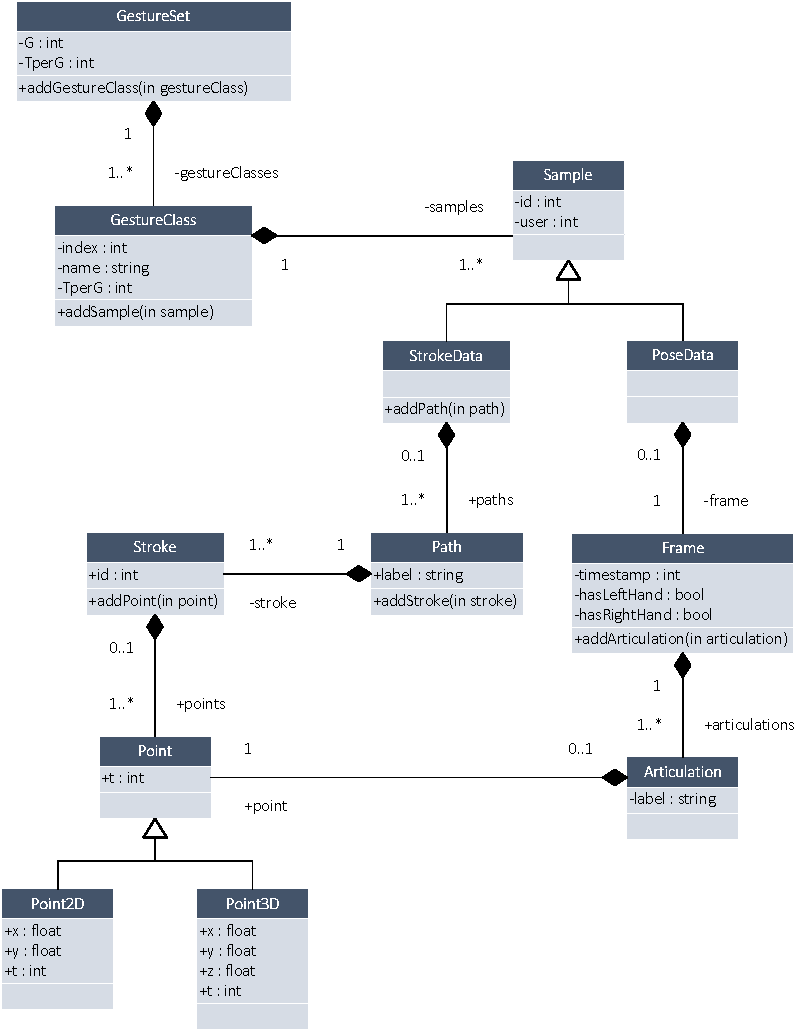
\includegraphics[width=\linewidth]{Figures/QuantumLeap/Architecture/QuantumLeap-UML.pdf}
    % \vspace{-4pt}
    \caption{UML V2.5 class diagram of the gesture sets.}
    \label{fig:quantumleap:dataset-uml}
    % \vspace{-12pt}
\end{figure*}
\fig~\ref{fig:quantumleap:dataset-uml} depicts the UML V2.5 \cite{Bush:2011} Class diagram of the modular data structure used in the framework. The \custominlinecode{GestureSet} object can contain samples of two types: (1) \custominlinecode{PoseData}, for static gestures consisting of a single frame that represents a hand pose; and (2) \custominlinecode{StrokeData}, for dynamic gestures, which comprise multiple paths, where a path corresponds to the trajectory~\cite{Caputo:2018} of a specific joint (\eg the tip of the right index). Paths are in turn decomposed into a series of strokes. Only one method is required:
\begin{itemize}[noitemsep]
    \item \custominlinecode{loadDataset(name, path, identifier)}: load a gesture dataset into memory as a \custominlinecode{GestureSet} object.
\end{itemize}
Developers have two possibilities for selecting a gesture set. They can create a custom gesture set with any specialized software, such as \textsc{Magic2}~\cite{Kohlsdorf:2011} or \textsc{GestMan}~\cite{Magrofuoco:2019a}, or via an LMC gesture recorder\footnote{We release the code of the LMC Gesture Recorder on GitHub at \url{https://github.com/sluyters/LeapGesturePlayback}.}. Another option is to pick one of the many publicly available datasets, such as SHREC2019~\cite{Caputo:2019}, and convert it into the standardized format to be considered in \ql.

\subsubsection{Static Recognizer}
The static recognizer module attempts to recognize static gestures at each frame. For each recognized gesture, the recognizer should compute a confidence score ranging from 0 to 1, where 1 indicates that it is absolutely confident that it has correctly identified the gesture. If the score is lower than a manually set threshold, the gesture is rejected. In the future, this threshold could be automatically computed by \ql for each gesture class based on the training dataset(s). Having a dedicated module for static gesture recognition allows using more efficient recognizers that are specialized for this task. This should thus result in increased accuracy and lower CPU usage. A static recognizer module should implement three methods:
\begin{itemize}[noitemsep]
    \item \custominlinecode{addGesture(name, frame)}: add a static gesture to the training set of this recognizer.
    \item \custominlinecode{removeGesture(name)}: remove a static gesture from the training set of this recognizer (including all of its samples).
    \item \custominlinecode{recognize(frame)}: determine the name of the static gesture performed in the frame given as argument.
\end{itemize}
To avoid accidentally triggering dynamic gestures while the user is performing a static gesture, the recognition of dynamic gestures is stopped when a static gesture is recognized. Two static recognizer modules are provided and described in Appendix~\ref{app:quantumleap-modules:static-recognizers}.

\subsubsection{Analyzer}
These modules extract additional data from the sensor frames, which can then be used inside applications. They can serve to offload heavy computation from the front-end to the \ql dataflow, to implement more advanced feature extraction techniques that would otherwise clutter the front-end application, or to remove sensor-dependent code from the application. Any analyzer module should implement two methods:
\begin{itemize}[noitemsep]
    \item \custominlinecode{analyze(frame)}: extract relevant information from a frame.
    \item \custominlinecode{reset()}: reset the internal state of the analyzer.
\end{itemize}
As analyzer modules are highly specific to the application, we expect developers to create their own modules. However, one simple module is provided and described in Appendix~\ref{app:quantumleap-modules:analyzers}.

\subsubsection{Segmenter}
The role of this module is to identify intentional dynamic gestures from a continuous stream of data. It analyzes frames one by one until it identifies a gesture. It then returns one or more lists of frames (\eg if it has multiple sliding windows), which are subsequently transformed into \custominlinecode{StrokeData} objects that are sent to the dynamic gesture recognizer for recognition. If multiple lists of frames are returned at the same time, only the gesture with the highest confidence score is kept.
The most appropriate method for gesture segmentation varies depending on the application, environment, and sensor(s). For instance, a simple sliding window segmenter could be appropriate for a multimedia application, while a more accurate technique may be required in environments where mistakes are costly, such as operating rooms. It is thus important to leave the choice of segmenter to the designer. A segmenter module should implement four methods:
\begin{itemize}[noitemsep]
    \item \custominlinecode{addGesture(name, sample)}: add a dynamic gesture to the training set of the segmenter.
    \item \custominlinecode{removeGesture(name)}: remove a dynamic gesture from the training set of the segmenter (including all of its samples).
    \item \custominlinecode{computeSegments(frame)}: process a frame and return one or more lists of frames (\ie segments) if the frame marks the ending of a gesture.
    \item \custominlinecode{notifyRecognition()}: notify the segmenter that a gesture has been recognized. The segmenter may use this information to take the coarticulation between two subsequent gestures into account (\eg by temporarily pausing gesture segmentation after a gesture is recognized).
\end{itemize}
Three different segmenters are provided and described in Appendix~\ref{app:quantumleap-modules:segmenters}.

\subsubsection{Dynamic Recognizer}
Distinct from the static recognizers, dynamic recognizers analyze sequences of frames instead of individual frames. They are thus called only when the segmenter detects an intended gesture, which limits CPU usage and reduces the number of false positives. As for the static recognizers, they should return a confidence score for each recognized gesture and implement three methods:
\begin{itemize}[noitemsep]
    \item \custominlinecode{addGesture(name, sample)}: add a gesture to the training set of this recognizer. 
    \item \custominlinecode{removeGesture(name)}: remove a gesture from the training set of this recognizer (including all of its samples).
    \item \custominlinecode{recognize(sample)}: determine the name of the gesture that corresponds to the candidate sample given as argument.
\end{itemize}
Ten dynamic recognizers are provided that cover multiple properties of gesture sets, such as uni- \vs multi-stroke and properties of invariance (see Appendix~\ref{app:quantumleap-modules:dynamic-recognizers}).

%--------------------------------------------------------------------------------%
\subsection{Configuration} \label{sec:quantumleap:description:configuration}

\begin{figure}[!b]
    \centering
    \begin{subfigure}{.49\textwidth}
        \centering
        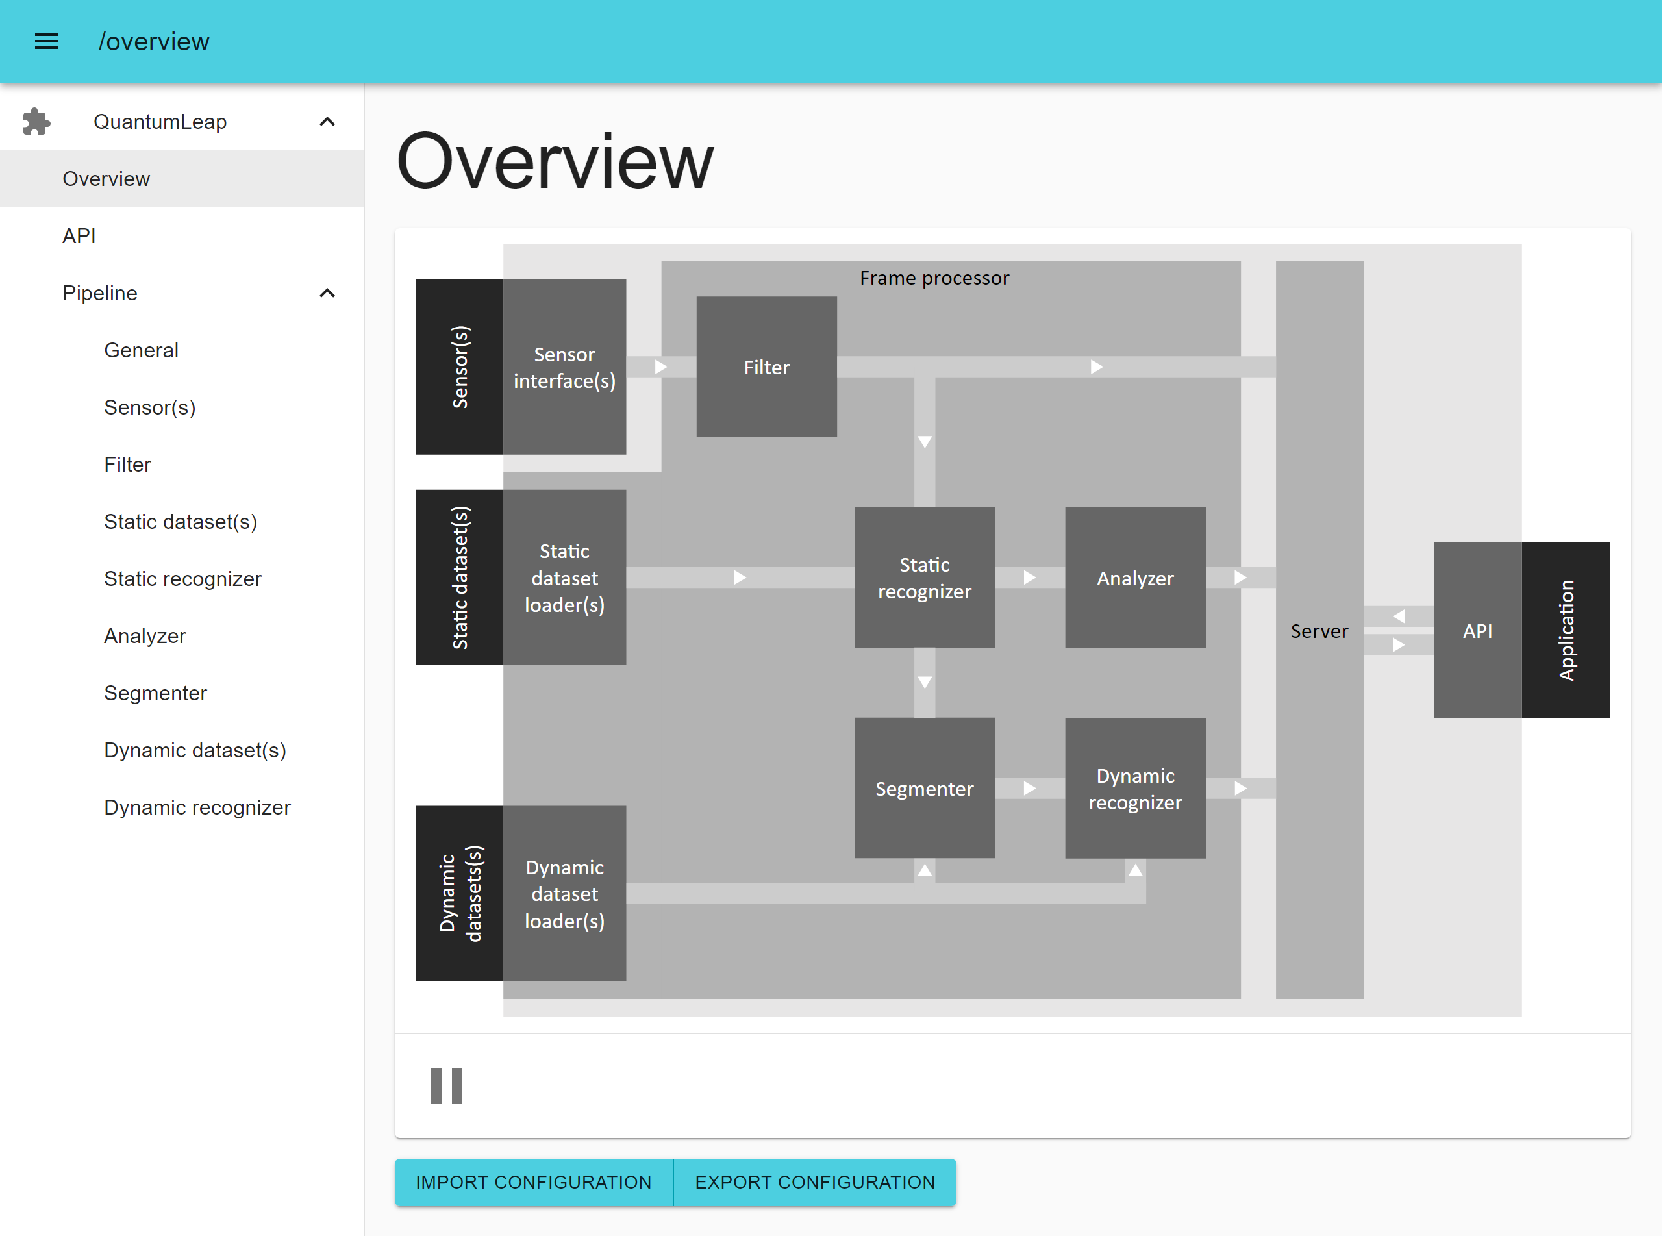
\includegraphics[width=\linewidth]{Figures/QuantumLeap/UI/overview.pdf}  
        \vspace{-15pt}
        \captionsetup{width=.9\linewidth}
        \caption{Overview.}
        \label{fig:quantumleap:ui:1}
    \end{subfigure}
    \begin{subfigure}{.49\textwidth}
        \centering
        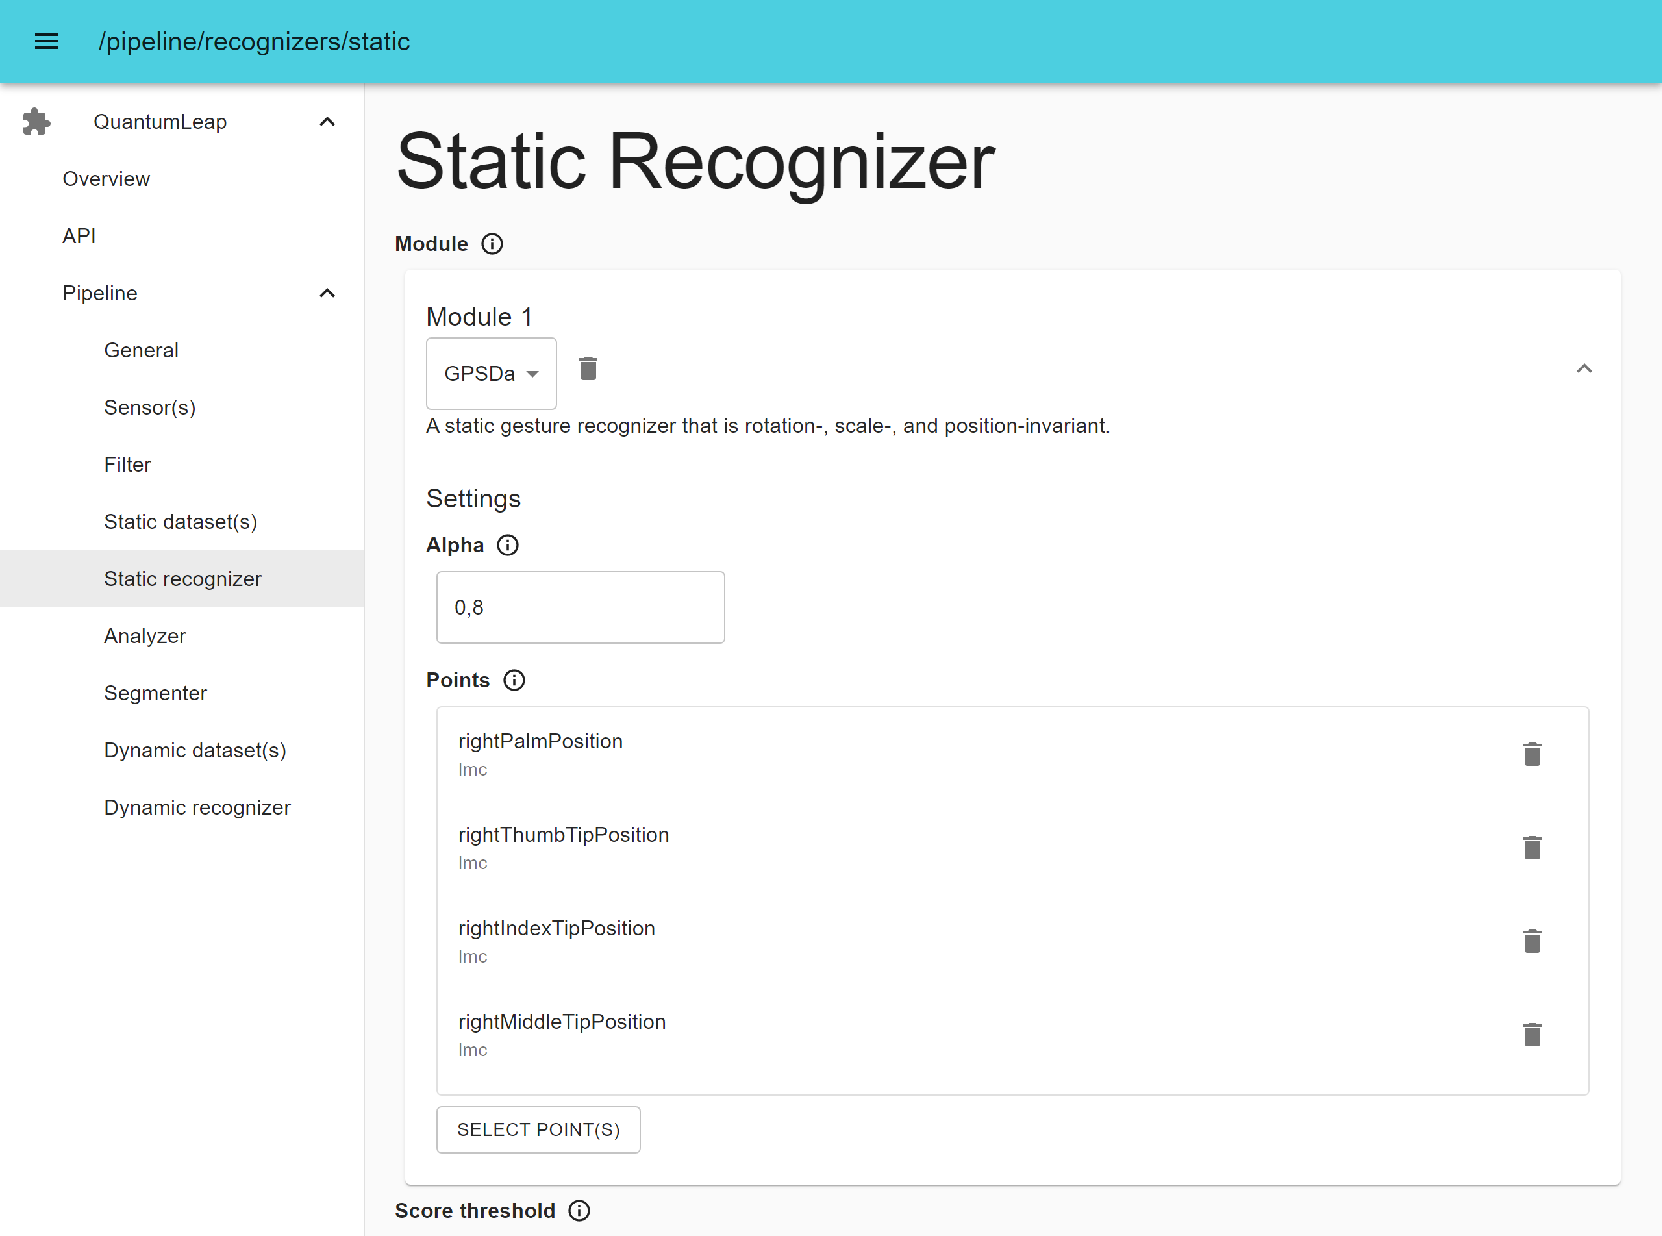
\includegraphics[width=\linewidth]{Figures/QuantumLeap/UI/module-static_recognizer.pdf}  
        \vspace{-15pt}
        \captionsetup{width=.9\linewidth}
        \caption{Static recognizer settings.}
        \label{fig:quantumleap:ui:3}
    \end{subfigure}
    
    \vspace{2pt}
    \begin{subfigure}{.49\textwidth}
        \centering
        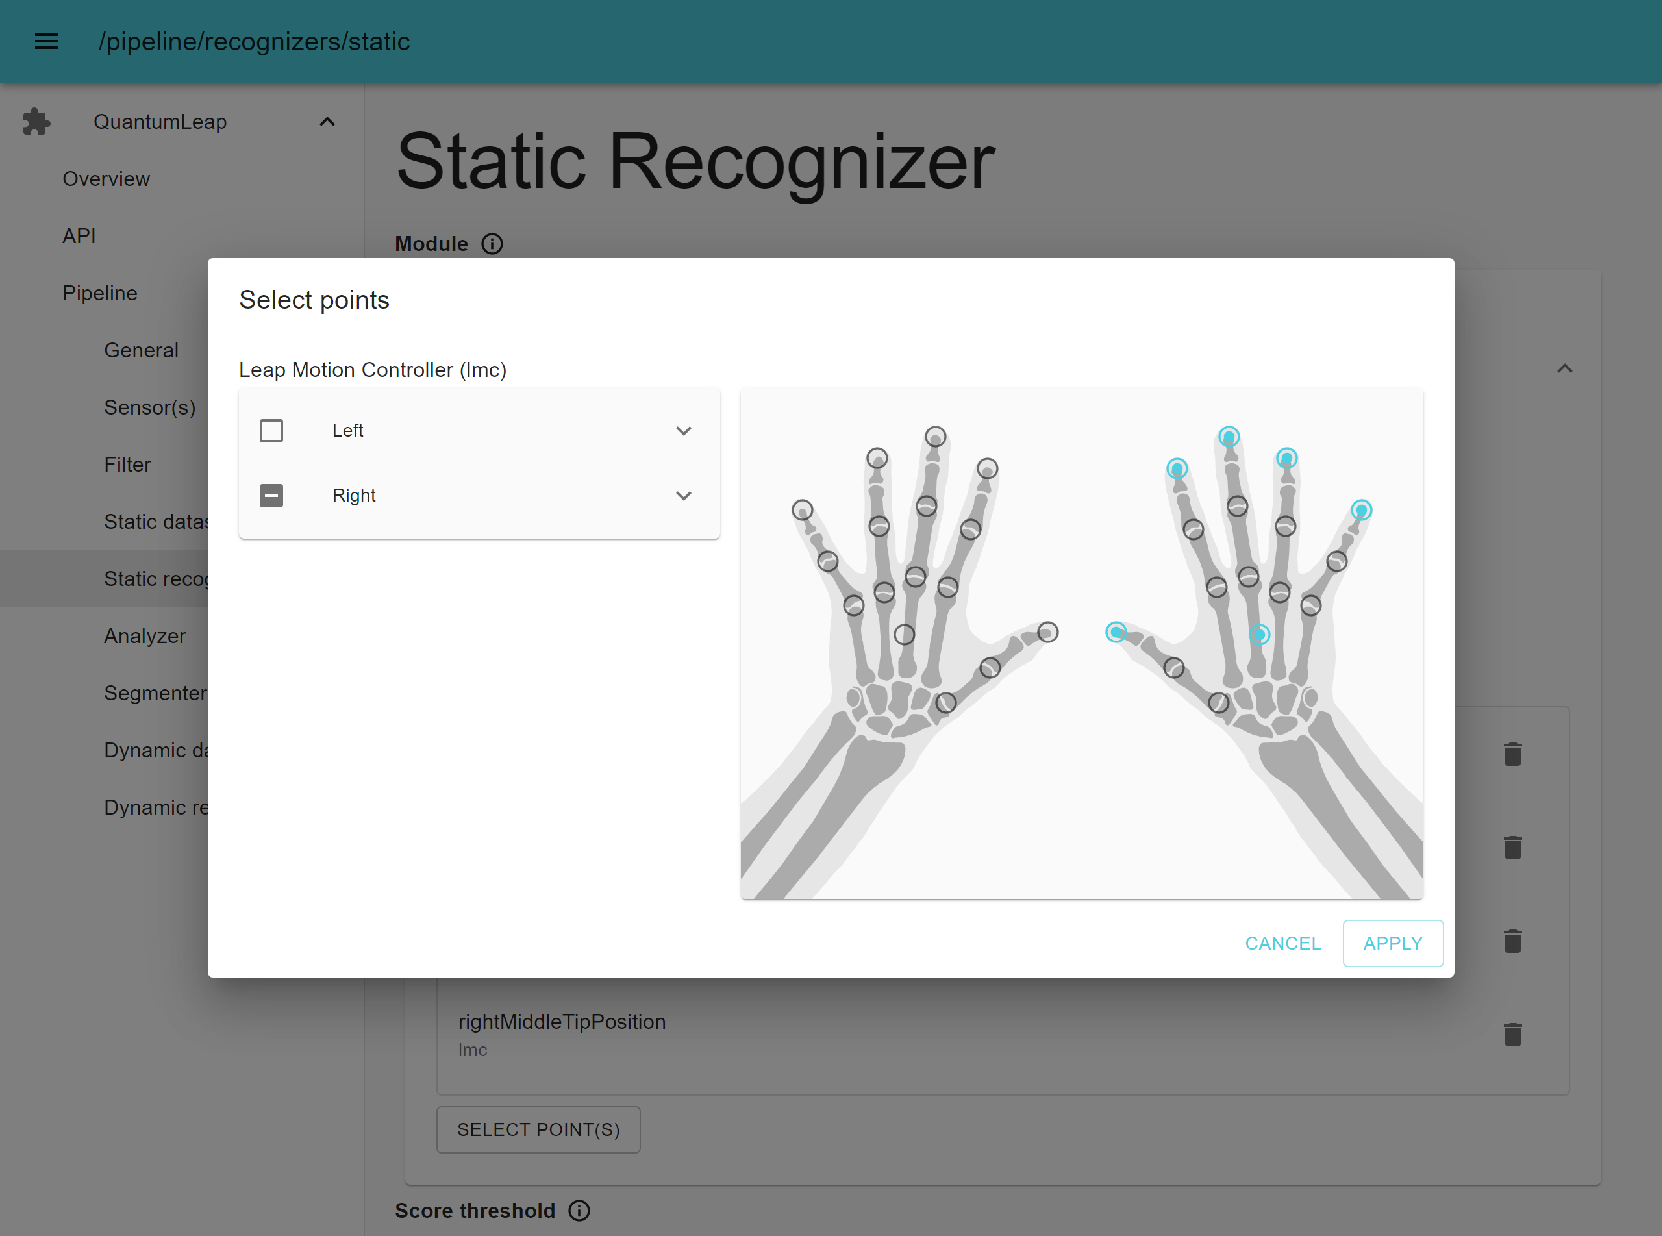
\includegraphics[width=\linewidth]{Figures/QuantumLeap/UI/module-point_selection.pdf}  
        \vspace{-15pt}
        \captionsetup{width=.9\linewidth}
        \caption{Point selection.}
        \label{fig:quantumleap:ui:4}
    \end{subfigure}
    \begin{subfigure}{.49\textwidth}
        \centering
        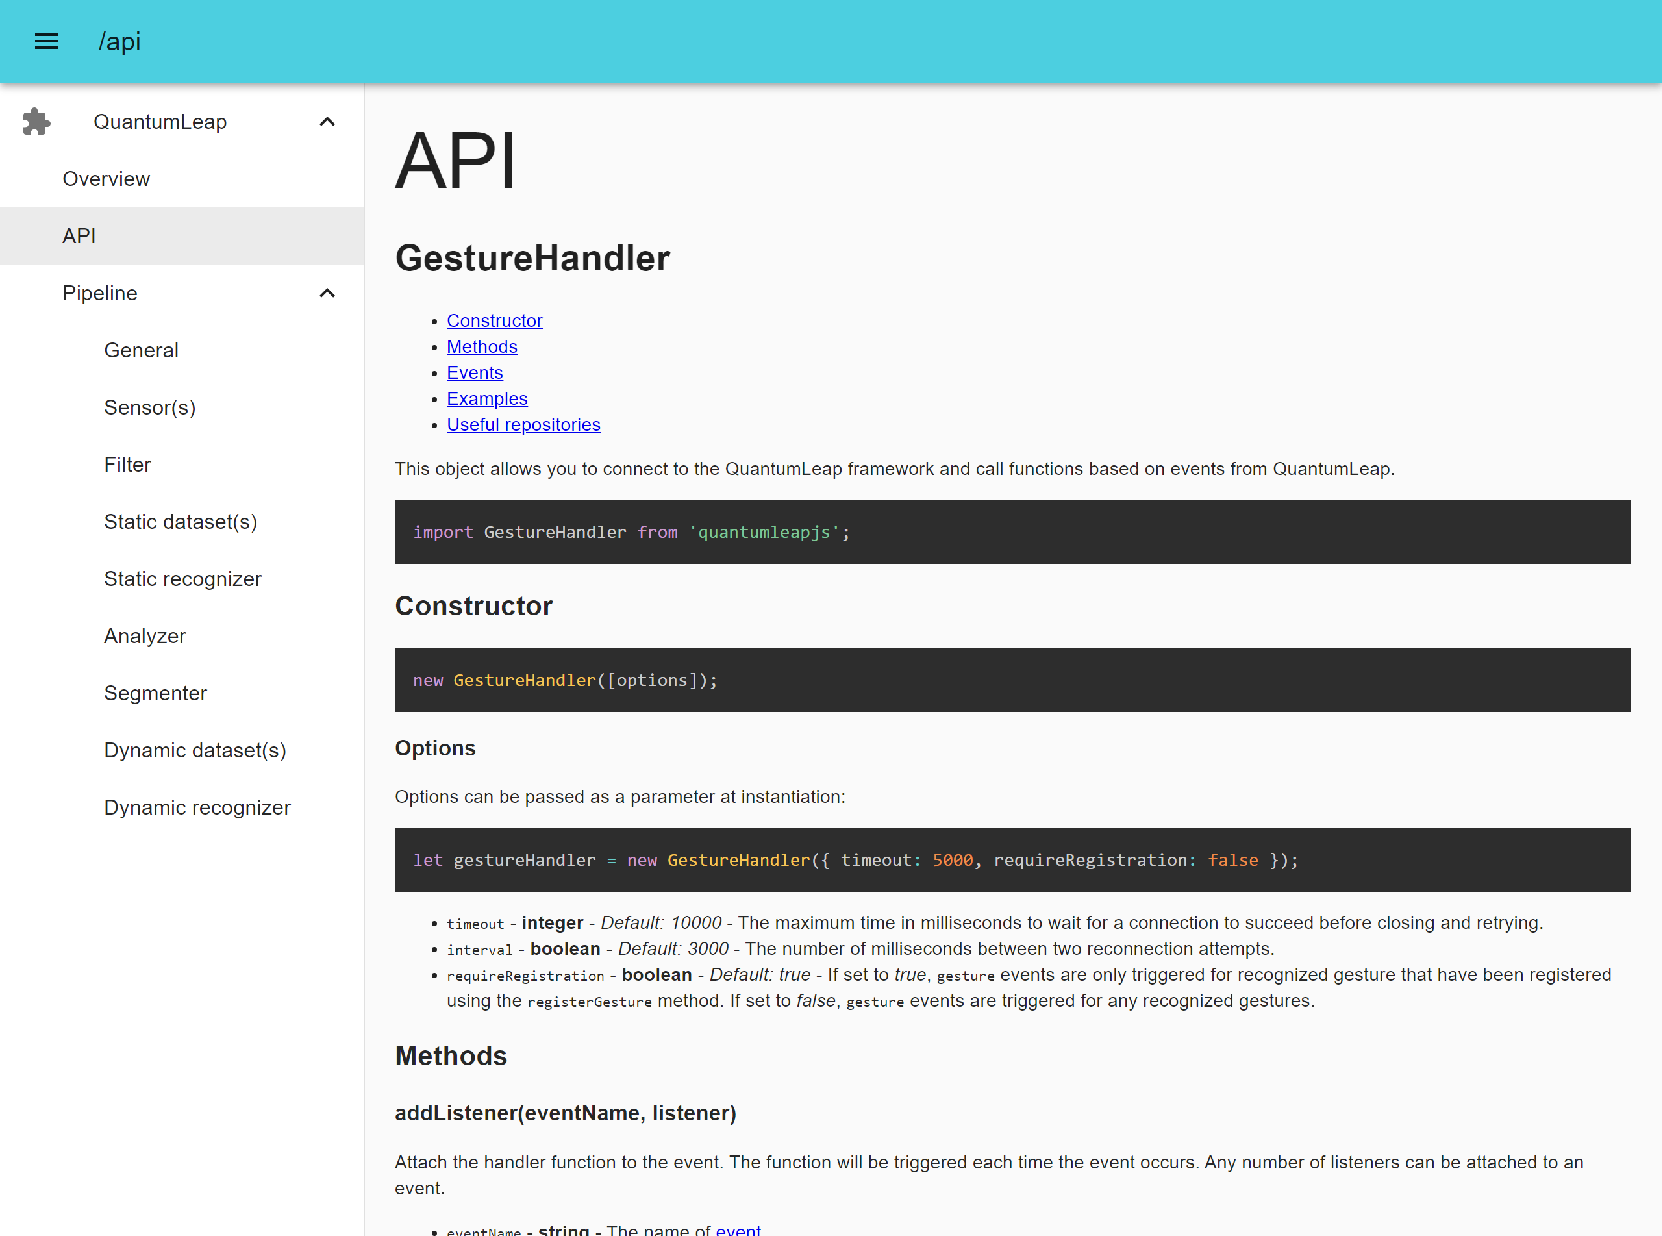
\includegraphics[width=\linewidth]{Figures/QuantumLeap/UI/api.pdf}  
        \vspace{-15pt}
        \captionsetup{width=.9\linewidth}
        \caption{API documentation.}
        \label{fig:quantumleap:ui:2}
    \end{subfigure}

    % \vspace{-4pt}
    \caption{Screenshots of the \ql GUI.}
    \label{fig:quantumleap:ui}
    % \vspace{-12pt}
\end{figure}

\ql features a configuration graphical user interface (GUI) that allows developers to quickly set it up for their needs. It is divided into a series of pages: an ``overview'' page which shows the complete dataflow architecture and allows users to navigate to the page of each module (\fig~\ref{fig:quantumleap:ui:1}), an ``API'' page that contains the complete API documentation (\fig~\ref{fig:quantumleap:ui:2}), and dedicated ``module'' pages for each type of module (\fig~\ref{fig:quantumleap:ui:3} and \ref{fig:quantumleap:ui:4}). The ``module'' pages let developers select a specific implementation of the module and configure it to their needs (\eg select the points used by a recognizer). The settings of each module can be defined in their corresponding ``config-template.json'' file. Framework configurations can be imported and exported as JSON files from the GUI.

The GUI provides limited guidance in the form of short descriptions for each implemented module to help developers select the best set of modules for their application. Further guidance, such as recommending the most appropriate modules (\eg gesture recognizers) for a particular application, is currently outside of the scope of this paper. 
However, resources like the comparative studies of Magrofuoco \etal~\cite{Magrofuoco:2021} or Erazo and P\'erez-Medina~\cite{Erazo:2020} may prove extremely valuable when choosing, \eg a gesture recognizer. 



%--------------------------------------------------------------------------------%
\subsection{Application Programming Interface} \label{sec:quantumleap:description:api}

The \ql API exposes the \custominlinecode{GestureHandler} class, a member of the \custominlinecode{EventEmitter} class of the Node.js core API. A \custominlinecode{GestureHandler} object attempts to connect to a running instance of the \ql framework. It then emits events based on the data received from \ql. %(\eg ``frame'' events are emitted for each frame received and ``gesture'' events are emitted for each recognized gesture). 
The reliance on a standard event-driven architecture should flatten the learning curve for front-end developers and facilitate the transition to gestural UIs, as events are already an integral part of modern UIs. The methods provided by the \custominlinecode{GestureHandler} class include:
\begin{itemize}[noitemsep]
    \item \custominlinecode{connect([address])}: connect to a running instance of \ql.
    \item \custominlinecode{disconnect()}: disconnect from \ql.
    \item \custominlinecode{registerGestures(type, names)}: register gestures to \ql, to enable their recognition.
    \item \custominlinecode{unregisterGestures(type, names)}: unregister gestures to stop them from being recognized.
    \item \custominlinecode{addListener(eventName, listener)}: attach a listener to a particular event. Possible events include:
    \begin{itemize}[noitemsep]
        \item \custominlinecode{frame}: a frame has been received from \ql.
        \item \custominlinecode{gesture}: a gesture (static or dynamic) has been recognized.
        \item \custominlinecode{connect}: the application has connected to \ql.
        \item \custominlinecode{disconnect}: the application has disconnected from \ql.
    \end{itemize}
    \item \custominlinecode{removeListener(eventName, listener)}: remove a listener attached to an event.
\end{itemize}

%================================================================================%
\section{Evaluation} \label{sec:quantumleap:evaluation}

The ISO 9241-Part 11~\cite{iso9241} defines the ``Usability'' quality factor appearing in the ISO 25010~\cite{iso25010} as ``\textit{the effectiveness, the efficiency,  and the satisfaction with which specified users achieve specified goals in particular environments}''. Therefore, to evaluate the overall usability of \ql, an experiment was conducted to quantitatively evaluate the task completion rate (to cover effectiveness), the task completion time, and the cognitive workload based on NASA-TLX~\cite{Hart:1988} (to cover efficiency), and the System Usability Scale (SUS)~\cite{Brooke:1996} to assess its overall usability (to also cover satisfaction). This section describes the evaluation procedure and discusses its results.

%--------------------------------------------------------------------------------%
\subsection{Experiment Protocol} \label{sec:quantumleap:evaluation:protocol}

\subsubsection{Environment}
Participants were sitting in front of a computer in a quiet room. An LMC was already set up and placed in front of them. Each participant was provided with two elements: 
\begin{itemize}
    \item A small React web application consists of four buttons linked to four gestures (``left swipe'', ``right swipe'', ``thumb'', and ``point index''). Clicking on a button displays the type, name, and image representation of the gesture on the screen.
    \item The \ql framework, including the documentation of its API. The configuration of the framework was reset before each experiment.
\end{itemize}

% \subsubsection{Consent}
% Before the experiment, participants were introduced to the procedure and informed that they could leave the experiment at any time. They were then invited to sign a GDPR-compliant consent form and fill in a demographic survey with their age, highest education level, current occupation, estimated number of years of experience in the field of computer science, and estimated expertise in development based on the nine expertise levels defined by Costabile \etal~\cite{Costabile:2008} (\fig~\ref{fig:quantumleap:expertise}).

\subsubsection{Participants}
A purposive and snowball sampling was used to recruit 7 participants (all males), aged between 21 and 27 years old ($M{=}23.3$, $SD{=}1.9$), who volunteered for the experiment. They reported between 1 and 7 years of experience in the field of computer science ($M{=}4.9$, $SD{=}2.2$), and expertise levels ranging from 5 to 9 ($M{=}7.6$, $SD{=}1.8$). Education levels included bachelor's degree (4 participants) and master's degree (3 participants). Our criteria for inclusion in this experiment required participants to have at least one year of professional development experience.

\subsubsection{Procedure and Tasks}
The experiment consisted of one session taking around 80 minutes per participant. A session consisted of six phases:

\begin{figure}[tb]
    \centering
    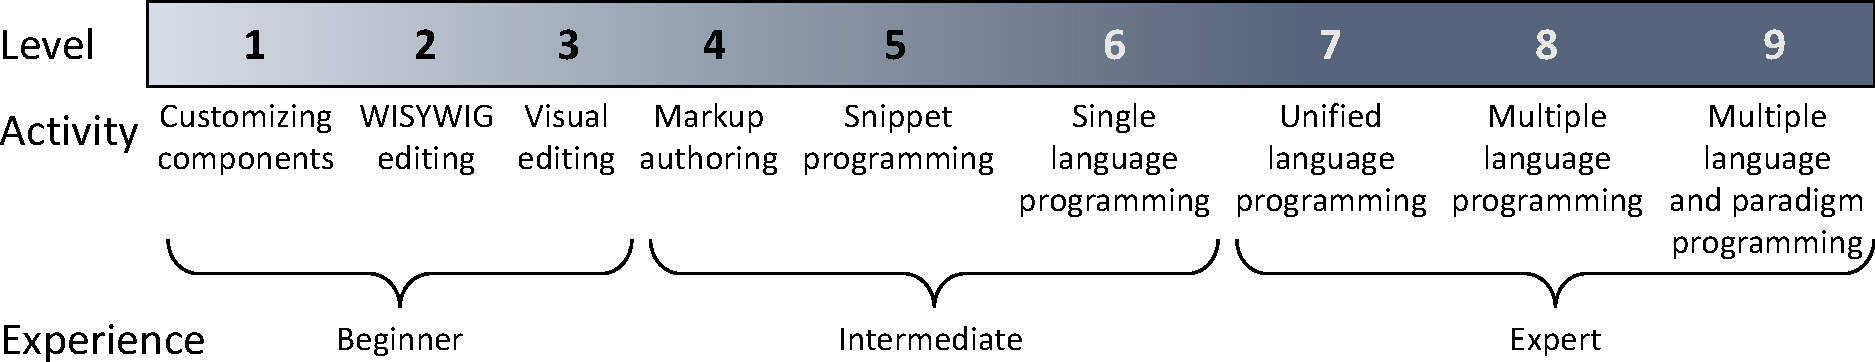
\includegraphics[width=\linewidth]{Figures/QuantumLeap/Evaluation/expertise-levels.pdf}
    \vspace{-8pt}
    \caption{The nine development expertise levels~\cite{Costabile:2008}.} %,Vanderdonckt:2019a}.}
    % \vspace{-8pt}
    \label{fig:quantumleap:expertise}
\end{figure}

\begin{enumerate}
    \item \textit{Consent form and demographic information.} Participants were introduced to the procedure and informed that they could leave the experiment at any time. They were then invited to sign a GDPR-compliant consent form and fill in a demographic survey with their age, highest education level, current occupation, estimated number of years of experience in the field of computer science, and estimated expertise in development based on the nine expertise levels defined by Costabile \etal~\cite{Costabile:2008} (\fig~\ref{fig:quantumleap:expertise}).
    \item \textit{Introduction phase.} Participants were introduced to the application and the \ql framework. They were given a few minutes to try them out and analyze the source code of the application before continuing the experiment.
    \item \textit{Configuration phase.} Participants configured the \ql framework for the application with its configuration GUI. This task comprised seven steps, detailed in Appendix~\ref{app:quantumleap-tasks:tasks-config}.
    \item \textit{Development phase.} Participants modified the source code of the application to make it react to static and dynamic hand gestures. This task comprised 13 steps, detailed in Appendix~\ref{app:quantumleap-tasks:tasks-dev}.
    \item \textit{Questionnaires.} Participants were asked to complete two questionnaires: the System Usability Scale (SUS) questionnaire~\cite{Brooke:1996} and the NASA-Task Load Index (NASA-TLX) questionnaire~\cite{Hart:1988}. 
    %
    SUS comprises ten questions evaluating the usability of a system (in this case, \ql) and has been selected for its proven reliability~\cite{Bangor:2008} and efficient administration. 
    %
    NASA-TLX assesses the estimated workload of the \textit{configuration} and \textit{development} tasks and comprises six subscales: mental demand, physical demand, temporal demand, effort, performance, and frustration level. Each subscale is assigned a weight determined by asking the participant to select the subscale that contributes the most to the workload in 15 pairwise comparisons. In this way, each participant was able to express which subscale is perceived as the most important with respect to others, as opposed to maintaining the same weight for all subscales. Pandian and Tuleri's NASA-TLX software~\cite{Pandian:2020} was used to simplify the process of data collection and analysis (\fig~\ref{fig:quantumleap:nasa-tlx-app}).
    \item \textit{Open-ended questions and comments.} Participants answered four questions to provide insights on their overall feelings:
    \begin{itemize}[noitemsep]
        \item If you did not complete all the tasks, what was the reason?
        \item What did you think of \ql?
        \item What did you like?
        \item What would you change?
    \end{itemize}
\end{enumerate}


% Participants were first introduced to the application and the \ql framework. They were given a few minutes to try them out and look at the source code of the application before continuing the experiment. The rest was divided into five tasks:
% \begin{enumerate}[noitemsep]
%     \item \textit{Configuration}: the participants configure the \ql framework for the application with its configuration UI. This task comprises 7 steps, detailed in Appendix~\ref{app:quantumleap-tasks:tasks-config}.
%     \item \textit{Development}: the participants modify the source code of the application to make it react to static and dynamic hand gestures. This task comprises 13 steps, detailed in Appendix~\ref{app:quantumleap-tasks:tasks-dev}.
%     \item \textit{SUS Questionnaire}: once the participants had finished the above two tasks and their related steps, they were asked to fill out the System Usability Scale (SUS) questionnaire~\cite{Brooke:1996}, which comprises ten questions evaluating the usability of a system (in this case, \ql). This questionnaire has been selected for its proven reliability~\cite{Bangor:2008} and its efficient administration.
%     \item \textit{NASA-TLX Questionnaire}: participants were then asked to fill out the NASA-Task Load Index (NASA-TLX) questionnaire~\cite{Hart:1988}, which assesses the estimated workload of the \textit{configuration} and \textit{development} tasks. It consists of six subscales: mental demand, physical demand, temporal demand, effort, performance, and frustration level. Each subscale is then assigned a weight that is determined by asking the participant to select the subscale that contributes the most to the workload in 15 pairwise comparisons. In this way, each participant was able to express which subscale is perceived as the most important with respect to others, as opposed to maintaining the same weight for all subscales. Pandian and Tuleri's NASA-TLX software~\cite{Pandian:2020} was used to simplify the process of data collection and analysis (\fig~\ref{fig:quantumleap:nasa-tlx-app}).
%     \item \textit{Open-Ended Questions and Comments}: the participants answer the following four open-ended questions to provide insights on their overall feelings:
%     \begin{itemize}[noitemsep]
%         \item If you did not complete all the tasks, what was the reason?
%         \item What did you think of \ql?
%         \item What did you like?
%         \item What would you change?
%     \end{itemize}
% \end{enumerate}

% Each evaluation took approximately ~80 minutes per participant.

\begin{figure}[h]
    \centering
    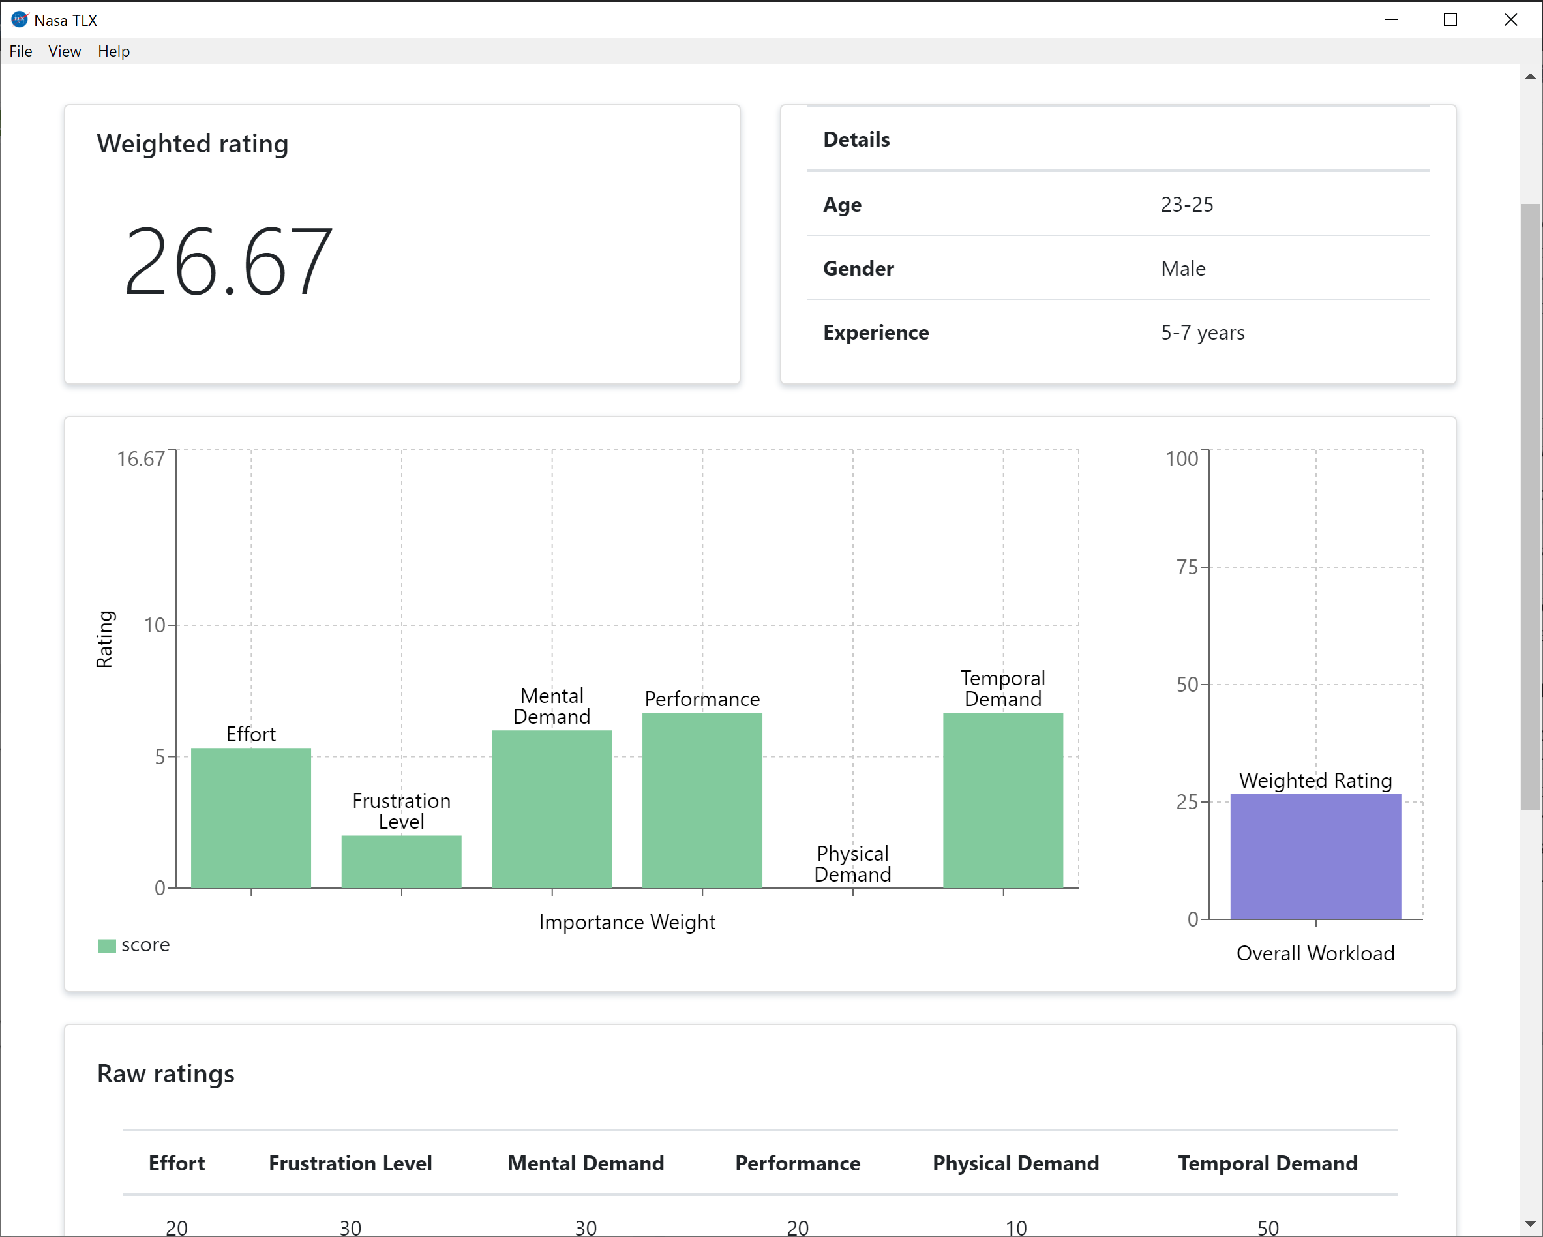
\includegraphics[width=\linewidth]{Figures/QuantumLeap/Evaluation/NASA-TLX.pdf}
    % \vspace{-8pt}
    \caption{NASA-TLX software~\cite{Pandian:2020} screenshot showing results of a participant: the overall weighted rating, the rating per subscale, and the individual weights for each subscale.}
    \label{fig:quantumleap:nasa-tlx-app}
    % \vspace{-8pt}
\end{figure}

\subsubsection{Metrics and Data Collection}
We collected a set of metrics for the configuration and development phases of the experiment to provide insight into the efficiency and effectiveness of \ql:
\begin{enumerate}
    \item The \textsc{Task success rate} is the ratio between the number of steps completed successfully by a participant and the total number of steps required to complete the procedure.
    \item The \textsc{Task completion time} measures the time taken by the participant for each of the configuration and development tasks.
    \item The \textsc{Step completion time} measures the time taken to perform each step of each of the two aforementioned tasks.
\end{enumerate}
In addition to these metrics, we collected demographic information, as well as answers to the SUS questionnaire, NASA-TLX questionnaire, and open-ended questions.

%--------------------------------------------------------------------------------%
\subsection{Results and Discussion} \label{sec:quantumleap:evaluation:results}

\subsubsection{Task Success Rate}
Despite their differences in terms of years of experience and level of expertise, six of the seven participants ($\frac{6}{7}{=}86\%$) completed all the steps of each task without any issue on the first run. Only one participant initially performed the fifth step of the \textit{Development} task incorrectly. However, this participant immediately realized his mistake and subsequently corrected it after completing the next step, ultimately resulting in a task success rate of 100\%. This suggests that the effectiveness is well covered by \ql.

\subsubsection{Task and Step Completion Times}
As a potential optimal performance, the first author of this paper (23 years, 6 years of experience, level 8)  completed the \textit{Configuration} and \textit{Development} tasks of the experiment in 2.1 minutes and 10.2 minutes, respectively. On average, participants took 6.6 minutes to complete the first task ($SD{=}1.2$), with the slowest participant completing it in 9.1 minutes and the fastest in 5.2 minutes. For the second task, the completion time was between 22.2 and 65.1 minutes ($M{=}37.4$, $SD{=}18.2$). \fig~\ref{fig:quantumleap:task2-time} shows that participants spent a more significant amount of time on the fifth step of this task (\ie adding an event listener that reacts to the ``swipe left'' gesture), which is normal since this is the most complex step.

\begin{figure}[t]
    \centering
    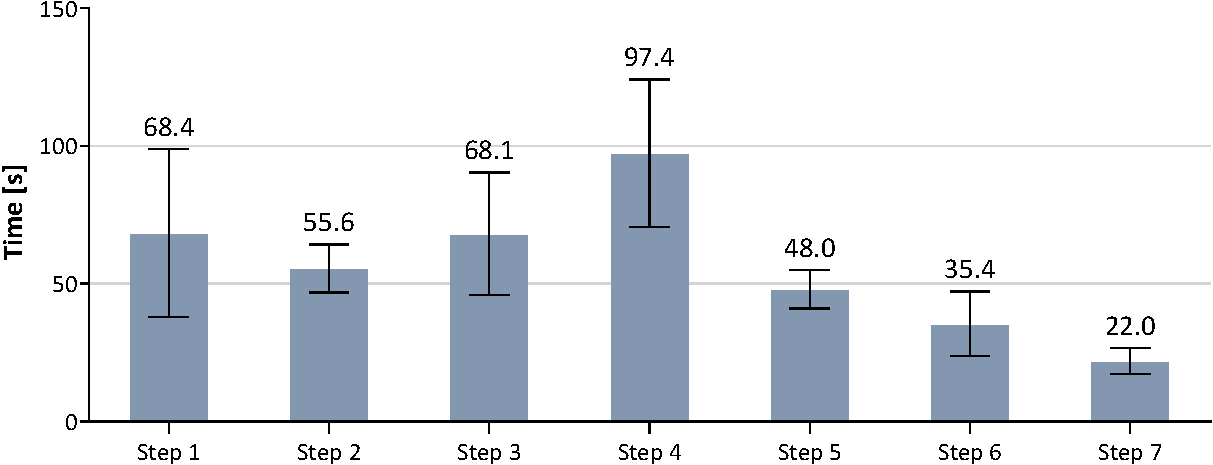
\includegraphics[width=\linewidth]{Figures/QuantumLeap/Evaluation/Task 1 (time).pdf}
    % \vspace{-14pt}
    \caption{Average time for each step of the \textit{Configuration} task. Error bars show a confidence interval with $\alpha{=}0.5$.}
    \label{fig:quantumleap:task1-time}
    % \vspace{-8pt}
\end{figure}


While steps five and eight are similar, participants took seven times longer to perform the former than the latter. A plausible explanation could be that the first time they encountered the problem of reacting to a gesture, participants took some time to check the API before modifying the source code of the application. When they mastered the API, participants could then quickly complete the remaining steps.


\begin{figure}[t]
    \centering
    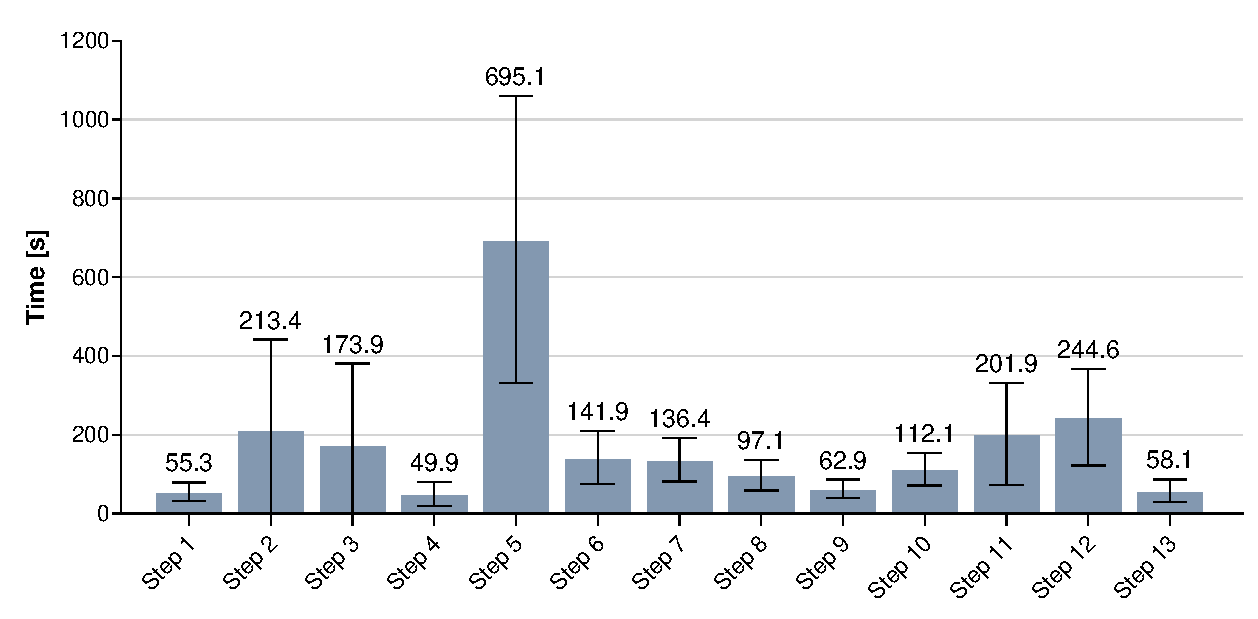
\includegraphics[width=\linewidth]{Figures/QuantumLeap/Evaluation/Task 2 (time).pdf}
    \vspace{-18pt}
    \caption{Average time for each step of the \textit{Development} task. Error bars show a confidence interval with $\alpha{=}0.5$. Note that one participant performed tasks 8, 9, and 10 in parallel. The participant's time for each of these tasks was thus inferred from the total time to perform the three tasks and the ratio between the average time for these tasks.}
    \label{fig:quantumleap:task2-time}
\end{figure}

To investigate the relationship between participants' expertise and their task completion time, we compute a Spearman's rank correlation between participants' reported level of expertise in development and their completion time for the \textit{Configuration} and \textit{Development} tasks. While no significant correlation was observed between the completion time of the first task and the expertise level, thus suggesting that the configuration GUI is perceived with a similar easiness regardless of the skill level, the completion time of the second task significantly correlates with expertise ($r{=}-.93$, $p{=}.002^{**}$). This result was expected, as the second task of the experiment requires participants to leverage their programming skills to modify the source code of the application. 

\subsubsection{SUS Questionnaire}
Since the answers to the SUS questionnaire were not normally distributed based on a Shapiro-Wilk test (\eg for question 3, $W{=}0.45$, $p{<}.001^{***}$), we investigated the overall appreciation of the participants by conducting a one-sample Wilcoxon test comparing their answers to the midpoint of the scale (\ie 3.0). For odd-numbered, resp. for even-numbered questions, an answer is considered positive if it is significantly higher, resp. lower than the midpoint value. All odd-numbered, resp. even-numbered, questions received a mean higher, resp. lower than the midpoint of the scale, thus representing an already positive assessment. Furthermore, six of the ten questions are statistically significantly different from the midpoint value, suggesting an even more positive answer for these questions: question 1 ($W{=}21.0$, $p{=}.031^*$), question 3 ($W{=}28.0$, $p{=}.016^*$), question 5 ($W{=}21.0$, $p{=}.031^*$), question 6 ($W{=}{-}21.0$, $p{=}.031^*$), question 7 ($W{=}28.0$, $p{=}.016^*$), and question 10 ($W{=}{-}21.0$, $p{=}.031^*$).
As recommended by Brooke~\cite{Brooke:1996} and Bangor \etal~\cite{Bangor:2008}, we also analyzed the SUS questionnaire as a whole. SUS scores range between 62.5 and 85.0 out of 100 ($M{=}77.9$, $SD{=}7.8$), resulting in a rating of B+ (``good'') on Sauro's rating scale~\cite{Sauro:2010}, which denotes a reasonable level of usability for such an environment. According to Lewis and Sauro~\cite{Lewis:2009}, the overall SUS score can be further divided into two subcomponents, namely learnability and usability. Learnability is computed by summing the scores of questions 4 and 10 of the questionnaire and multiplying the result by 12.5. Usability is computed by summing the scores of the other questions and multiplying the result by 3.125. QuantumLeap obtains a mean learnability score of 78.6 and a usability score of 77.7. 

To investigate the internal consistency reliability among participants, we also computed Guttman's $\lambda_4{=}.91$ coefficient~\cite{Guttman:1945} with $n{=}2,000$ iterations. This value is above $\lambda_4{\geq}.90$ which represents the highest rank of consistency, usually required for high-stakes decisions like school admissions~\cite{Callender:1979}, thus suggesting that participants consistently answered the SUS questionnaire and that their answers were reliable enough.
Guttman’s $\lambda_4$ coefficient represents a good measure of reliability that produces a  value higher than the usual Cronbach’s $\alpha$, but with a positive bias likely to be small if the estimated reliability is larger than 0.85 (which is the case here) when the sample is small ($n{=}7$). After computing the Spearman's rank correlation between participants' SUS scores and their reported level of expertise, we observe a positive correlation ($r{=}.82$, $p{=}.033^*$), which suggests that the system feels more usable to experienced users than to intermediary ones.

\subsubsection{NASA-TLX Questionnaire}
% Graph with weighted scores
Workload scores range from 8.7 to 65.3 out of 100 ($M{=}34.0$, $SD{=}19.5$). According to Grier~\cite{Grier:2015}, who analyzed the NASA-TLX scores of 37 computer activities, the measured workload for \ql falls into the second quartile (score lower than 54.0). Each participant managed to complete all steps of the experiment and some even reported being impressed by the results, considering that they would not have been able to do the same without the help of the framework. This could explain the low impact of the ``performance subfactor''. 
 Contrarily to the SUS score, no significant correlation was observed between participants' workload scores and their reported level of expertise after computing Spearman's rank correlation.

\begin{figure}[t]
    \centering
    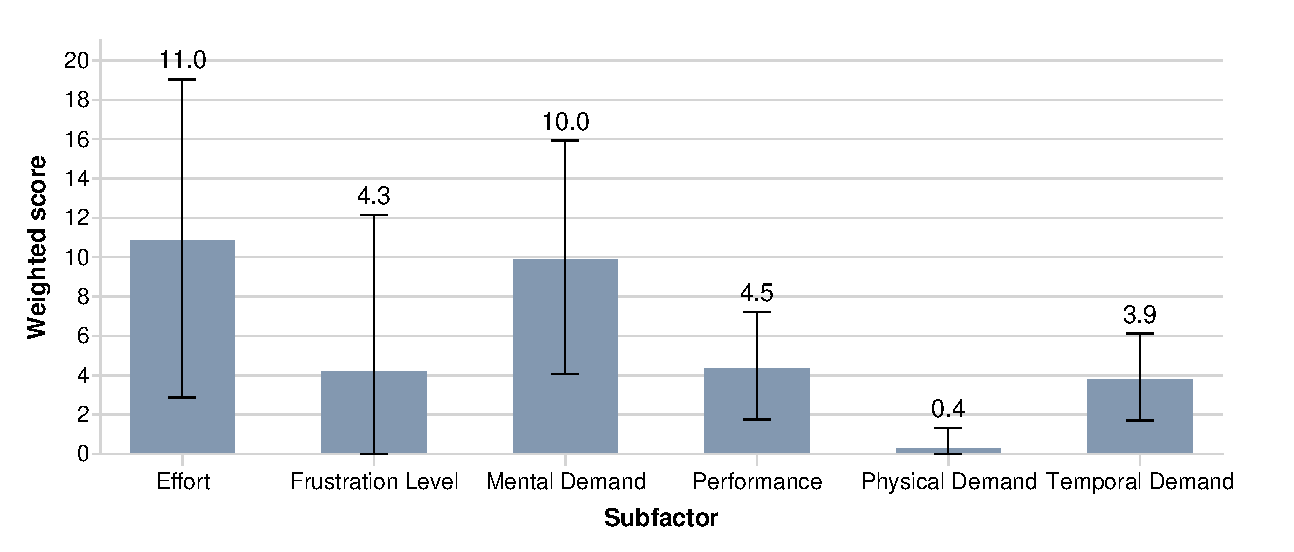
\includegraphics[width=\linewidth]{Figures/QuantumLeap/Evaluation/NASA-TLX-scores.pdf}
    \vspace{-16pt}
    \caption{Average weighted score for each subscale of the NASA-TLX questionnaire. Error bars show a confidence interval with $\alpha{=}0.5$.}
    % \vspace{-8pt}
    \label{fig:quantumleap:nasa-tlx-scores}
\end{figure}

\begin{table}[t]
    \footnotesize
    \centering
    \begin{tabular}{lrr}
        \toprule
        \multirow{2}{*}{\textbf{Subscale}} & \multicolumn{2}{c}{\textbf{Score}} \\
         & M & SD \\
        \midrule
        Mental Demand & 10.0 & 6.4 \\
        Physical Demand & 0.4 & 1.0 \\
        Temporal Demand & 3.9 & 2.4 \\
        Effort & 11.0 & 8.7 \\
        Performance & 4.5 & 2.9 \\
        Frustration level & 4.3 & 8.5 \\
        \midrule
        Overall & 34.0 & 19.5 \\
        \bottomrule
    \end{tabular}
    \caption{Average weighted score and standard deviation for each subscale of the NASA-TLX questionnaire.}
    % \vspace{-18pt}
    \label{tbl:quantumleap:nasa-tlx}
\end{table}

\subsubsection{Open-Ended Questions}
Overall, participants found that adding gesture support to an application was surprisingly quick and easy. However, some participants expressed some concern about not being able to configure the dataflow correctly without external help. Their remarks and suggestions are summarized as follows:
\begin{enumerate}[noitemsep]
    \item \textit{Configuration}. Comments targeting the configuration process, the GUI, and the usability.
    \begin{itemize}[noitemsep]
        \item There should be some feedback to indicate to the user that the framework is starting/stopping ($\frac{6}{7}{=}86\%$). 
        \item There should be some feedback to notify the user that the settings were successfully saved ($\frac{5}{7}{=}71\%$).
        \item After selecting a module, its settings should be displayed by default, instead of having to click to display them ($\frac{5}{7}{=}71\%$).
        \item A lot of steps are required to configure the dataflow ($\frac{2}{7}{=}29\%$).
        \item There should be a button to add a module, instead of just selecting the module in a drop-down menu ($\frac{2}{7}{=}29\%$).
        \item There should be a tutorial that provides guidance on dataflow configuration ($\frac{1}{7}{=}14\%$).
        \item There are some inconsistencies in the GUI ($\frac{1}{7}{=}14\%$).
        \item There should be a simple way to switch from right-handed gestures to left-handed ($\frac{1}{7}{=}14\%$).
    \end{itemize}
    \item \textit{Development}. Comments targeting the development of a gesture-based application using the \ql API.
    \begin{itemize}[noitemsep]
        \item There should be a method to directly attach a listener to a specific gesture, instead of having to listen to the generic ``gesture'' event and then check the gesture name ($\frac{2}{7}{=}29\%$).
        \item The API documentation should provide the data types of event properties ($\frac{1}{7}{=}14\%$).
        \item The API documentation should clearly show the link between listeners and events ($\frac{1}{7}{=}14\%$).
        \item The distinction between static and dynamic gestures may be confusing ($\frac{1}{7}{=}14\%$).
    \end{itemize}
    \item \textit{Experiment} Comments targeting the experiment itself (\eg unclear steps).
    \begin{itemize}[noitemsep]
        \item The order of some steps was confusing. In particular, the call to \custominlinecode{registerGesture} should have been introduced before the call to \custominlinecode{addListener} ($\frac{2}{7}{=}29\%$). 
        \item In step three of the second task, the address and port of the running instance of \ql should have been provided ($\frac{2}{7}{=}29\%$). 
    \end{itemize}
\end{enumerate}

\subsubsection{Limitations of the Study}
This study is subject to two main limitations, which could influence the validity of its outcomes.
%
First, the substantial guidance provided during the ``configuration'' phase of the study poses a threat to its external validity~\cite{Feldt:2010}, as our findings may not generalize to a real-life scenario in which no such guidance is available. 
%
Second, the study would have benefited from incorporating an A/B comparison between the development of a gesture-based application with and without \ql to better highlight its impact in terms of time, effort, and the overall quality of the resulting work.

%--------------------------------------------------------------------------------%
\subsection{Changes} \label{sec:quantumleap:evaluation:changes}
Following this experiment, we are planning on improving \ql based on the aforementioned participants' comments.

\subsubsection{Short-term Changes} The most requested changes have already been implemented in the latest version of \ql. They include:
\begin{itemize}
    \item Displaying a loading icon in the GUI when \ql is starting\slash stopping.
    \item Displaying a message in the GUI when the settings have been saved.
    \item Displaying the settings of modules by default in the GUI, instead of requiring the user to click on a button to display them.
\end{itemize}

\subsubsection{Long-term Changes} 
We believe that these long-term changes would prove especially useful for less experienced developers:
\begin{itemize}
    \item Add the possibility to attach listeners to specific gestures in one step, instead of requiring developers to listen to the generic ``gesture'' event.
    \item Propose a set of default configurations to allow developers to quickly prototype gesture-enabled applications without having to build a complete dataflow configuration.
    \item Create an interactive tutorial that guides users through the configuration of the \ql dataflow.
    \item Automatically configure the dataflow based on the selected gesture set and target usage. For instance, \ql could suggest a segmenter that is well-suited to the environment and determine the most accurate recognizers for the gesture set.
\end{itemize}


%================================================================================%
\section{Sensor Integration and Applications} \label{sec:quantumleap:integration}
Through the years, additional sensors were implemented into \ql by students for use in their master's thesis, showing that \ql can be easily extended with new modules. These sensors and some of their applications are summarized in \tab~\ref{tab:quantumleap:integration}.

In this thesis, we used \ql to build an LMC-based multimedia application called Large User Interface (\lui, \fig~\ref{fig:quantumleap:apps:lui}~\cite{Sluyters:2022:LUI}. This application, its user-centered development method, and its evaluation are described in Chapter~\ref{chap:lui}.
%
With the help of my friends and colleagues Quentin Sellier, Victor Slu\"{y}ters, and Jean-Martin Vlaeminck, we also used \ql during the Citizens of Wallonia hackathon in March 2023 to create Wall'ON (\fig~\ref{fig:quantumleap:apps:wallon}), an interactive kiosk that provides information about works in the city in a fun and intuitive way~\cite{Rawart:2023}.

\begin{table}[!b]
    \renewcommand{\arraystretch}{1.2}
    \footnotesize
    \centering
    \begin{tabular}{l>{\raggedright}p{2.5cm}>{\raggedright}p{1.75cm}ll}
        \toprule    
        \textbf{Sensor(s)} & \textbf{Type} & \textbf{Application Domain} & \textbf{Validation} & \textbf{Reference} \\
        \midrule
        Leap Motion Controller & Vision & Multimedia & S, D, U & This work \\
         &  & Healthcare & S, D & \cite{Nothomb:2020} \\
         &  & Participatory governance & D & \cite{Rawart:2023} \\
        Kinemic & IMUs & Multimedia & S, D & \cite{Steeman:2022} \\
        3D Touchpad & Touch + proximity sensor & N/A & S & \cite{Neuville:2021} \\
        Gheran Ring Device & IMUs & N/A & S & \cite{Lahousse:2022} \\
        Myo Armband & EMG & N/A & S & \cite{Cornet:2023} \\
        Touchscreen & Touch & Smart home & S, D & \cite{Moinnet:2022} \\
        \bottomrule
    \end{tabular}
    \caption{Summary of the sensors included into \ql. Types of validation include system performance (S), demonstration (D), and user study (U).}
    \label{tab:quantumleap:integration}
\end{table}

Nothomb \etal~\cite{Nothomb:2020} introduced a gesture-based DICOM image viewer (\fig~\ref{fig:quantumleap:apps:dicom}) that allowed surgeons to navigate patient images in the operating room more hygienically and efficiently.
%
Chauvaux and Steeman~\cite{Steeman:2022} integrated the Kinemic sensor, an armband that uses Inertial Measurement Units (IMUs) to track arm gestures, into \ql and built a gesture-based presentation application in which users could change slides with simple hand gestures (\fig~\ref{fig:quantumleap:apps:slides}).
%
Gosselin and Moinnet~\cite{Moinnet:2022} used \ql to build a touch-based application that enabled users to record and assign (combinations of) stroke gestures to actions in a smart house, such as turning the lights on (\fig~\ref{fig:quantumleap:apps:smart-home}).

Finally, Neuville~\cite{Neuville:2021}, Lahousse~\cite{Lahousse:2022}, and Cornet~\cite{Cornet:2023} integrated three additional sensors into \ql: (1) the 3D Touchpad, a device that supports touch and 3D gestures performed above its surface, (2) the Phidget ring, which captures 3D hand motion with an accelerometer, and (3) the Myo Armband, an EMG sensor that fits around the arm. They did not develop any application but used \ql to compare various recognizer modules on their gesture set.

\begin{figure}[t]
    \centering
    \begin{subfigure}{.259\textwidth}
        \centering
        \includegraphics[width=\linewidth]{Figures/QuantumLeap/Applications/lui-prototype.pdf}  
        \vspace{-15pt}
        \captionsetup{width=.9\linewidth}
        \caption{LUI.}
        \label{fig:quantumleap:apps:lui}
    \end{subfigure}
    \begin{subfigure}{.337\textwidth}
        \centering
        \includegraphics[width=\linewidth,trim={5cm 0 0 0},clip]{Figures/QuantumLeap/Applications/wallon-prototype.pdf}  
        \vspace{-15pt}
        \captionsetup{width=.9\linewidth}
        \caption{Wall'ON.}
        \label{fig:quantumleap:apps:wallon}
    \end{subfigure}
    \begin{subfigure}{.383\textwidth}
        \centering
        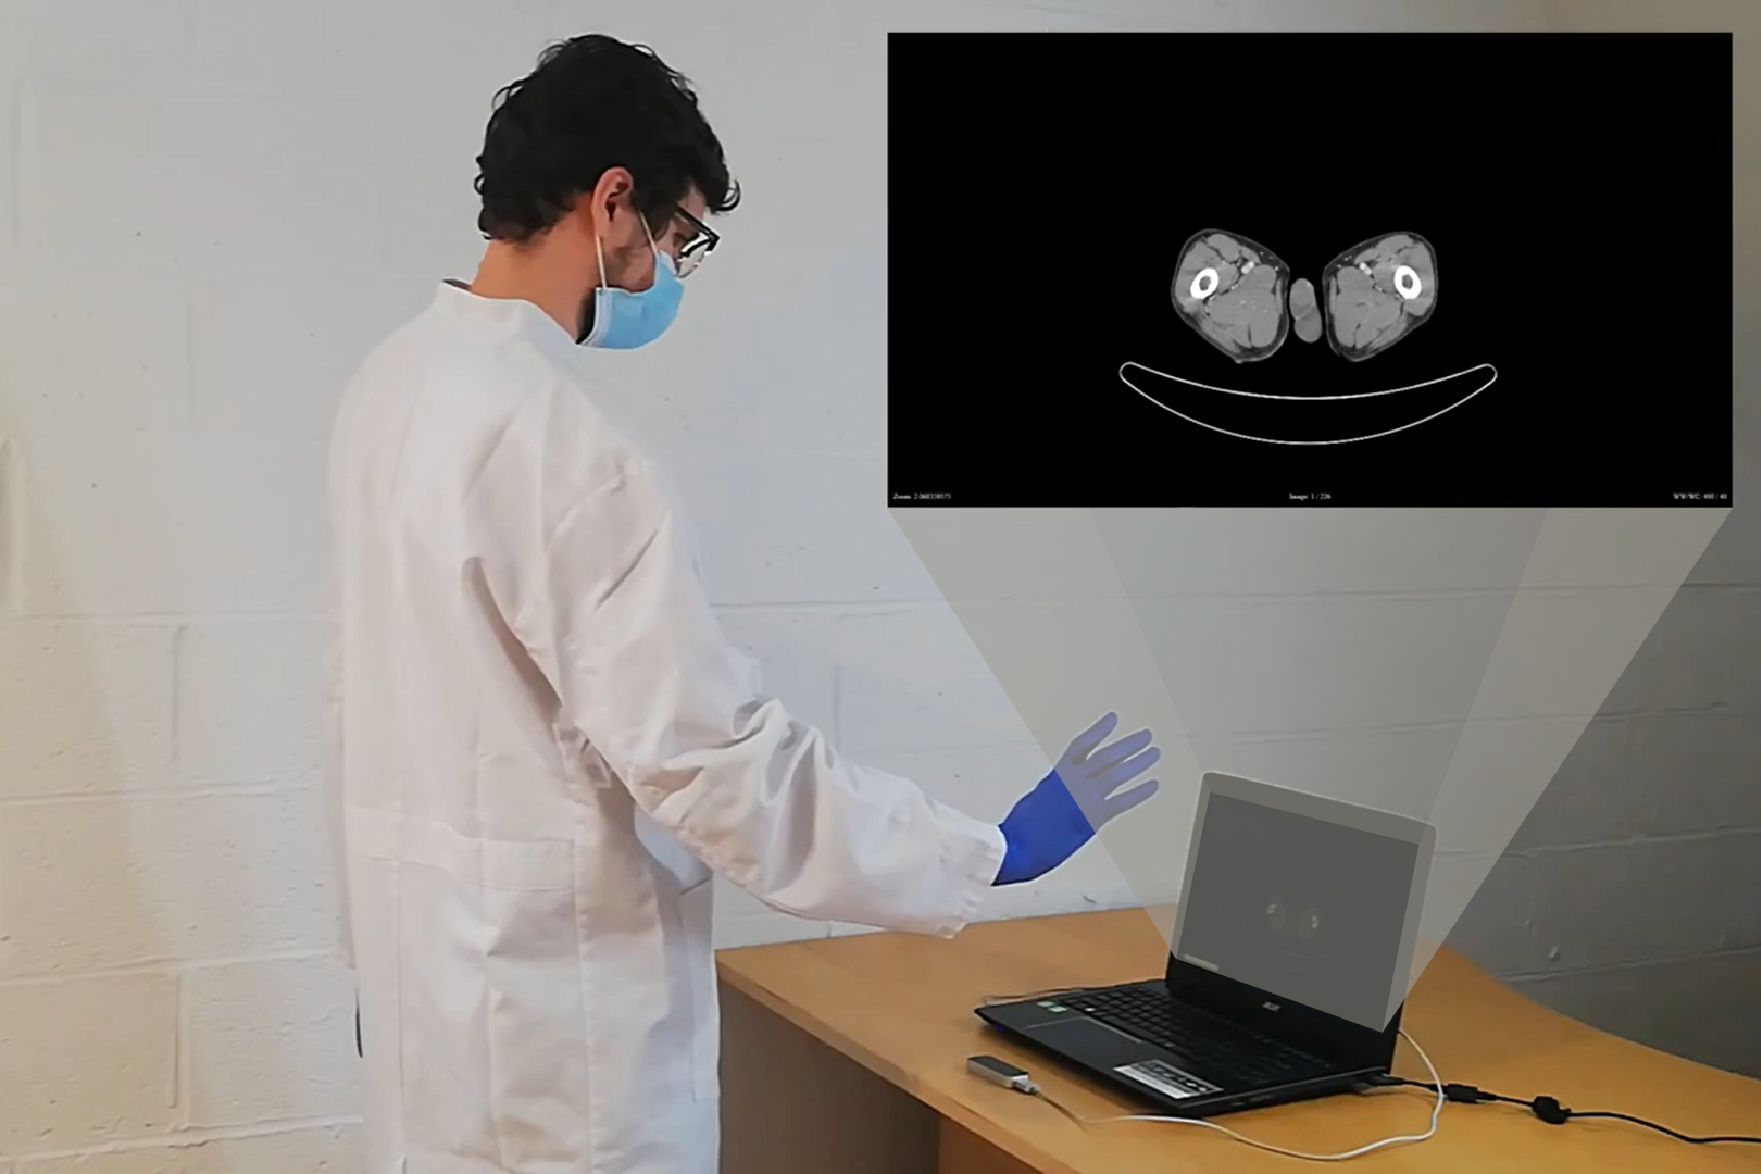
\includegraphics[width=\linewidth,trim={4.5cm 0 0 0},clip]{Figures/QuantumLeap/Applications/dicom-prototype.pdf}  
        \vspace{-15pt}
        \captionsetup{width=.9\linewidth}
        \caption{DICOM viewer~\cite{Nothomb:2020}.}
        \label{fig:quantumleap:apps:dicom}
    \end{subfigure}

    \vspace{2pt}
    \begin{subfigure}{.455\textwidth}
        \centering
        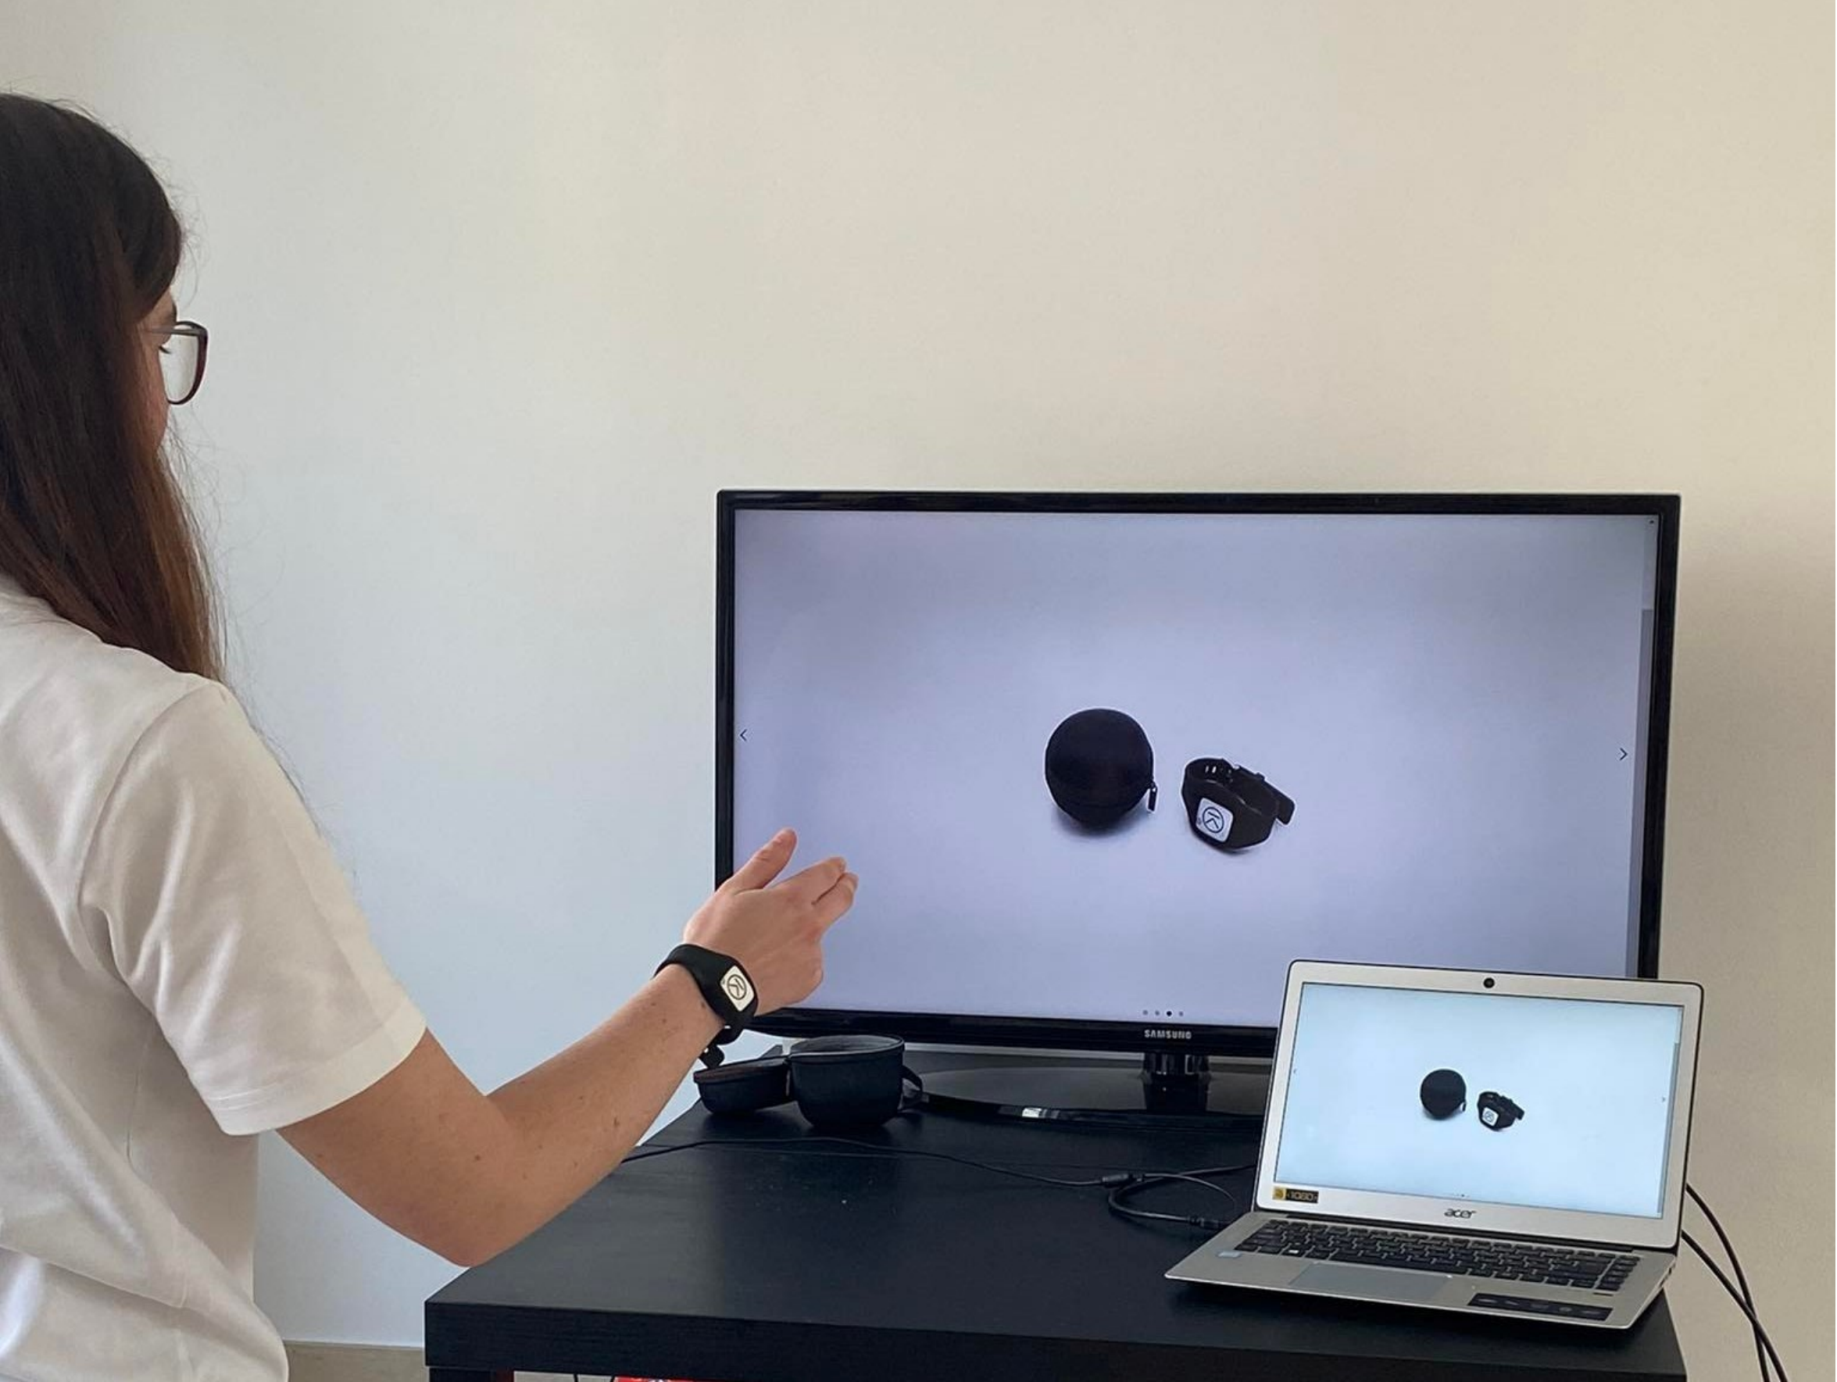
\includegraphics[width=\linewidth,trim={0 0 1cm 0cm},clip]{Figures/QuantumLeap/Applications/slides-prototype.pdf}  
        \vspace{-15pt}
        \captionsetup{width=.9\linewidth}
        \caption{Slides application~\cite{Steeman:2022}.}
        \label{fig:quantumleap:apps:slides}
    \end{subfigure}
    \begin{subfigure}{.535\textwidth}
        \centering
        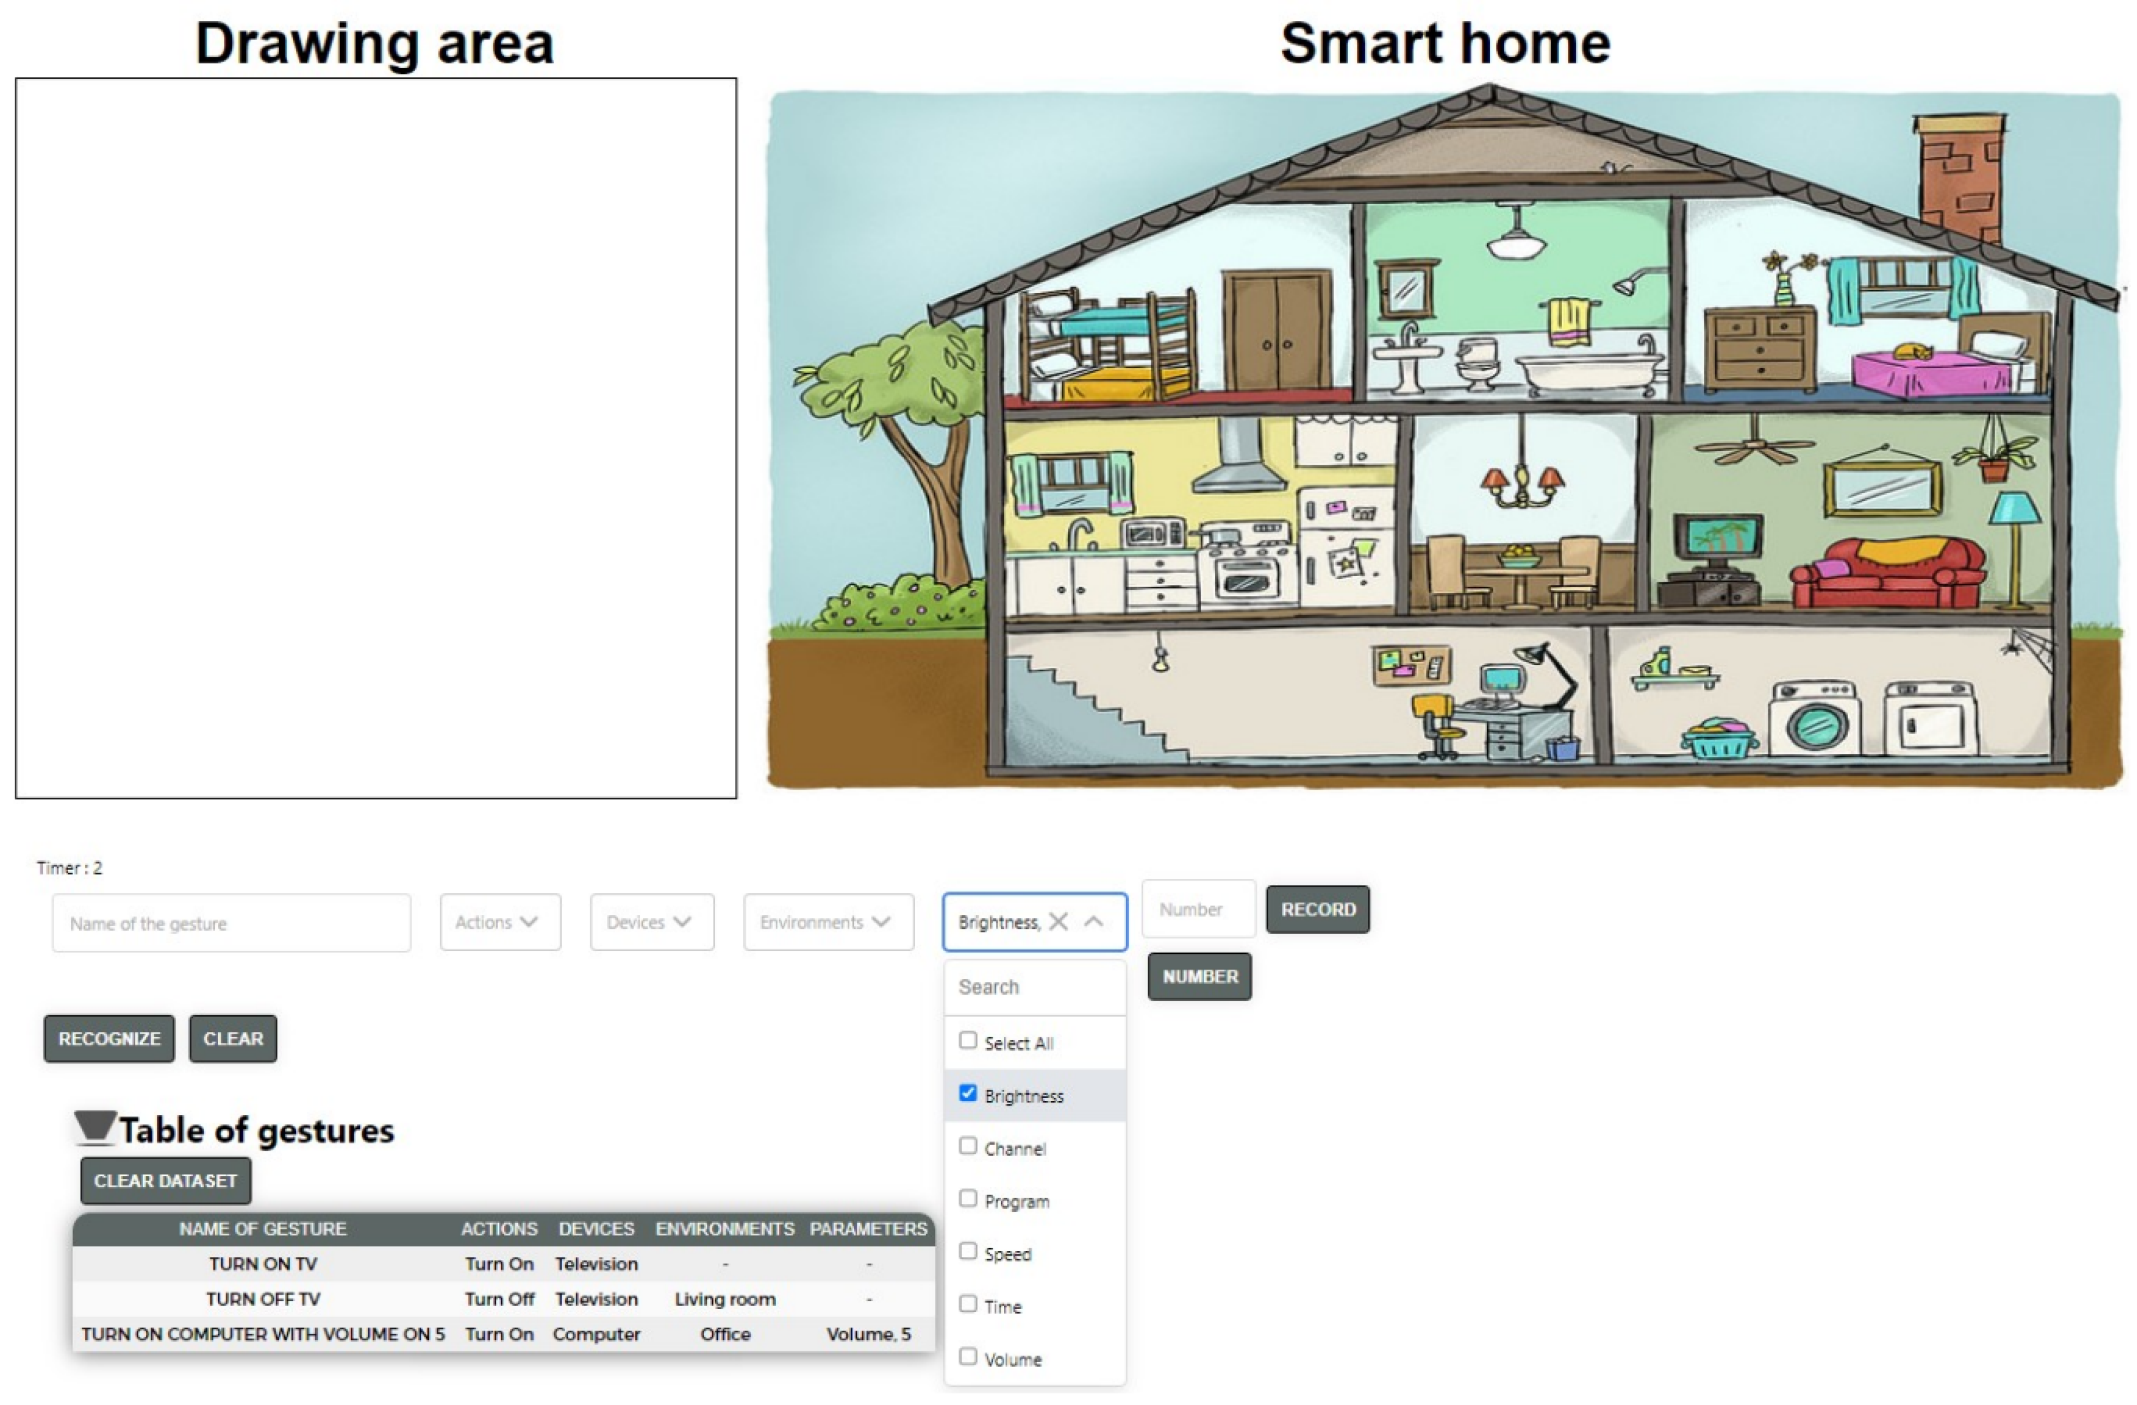
\includegraphics[width=\linewidth,trim={0.1cm 0.1cm 0.1cm 0.1cm},clip]{Figures/QuantumLeap/Applications/smart-home-prototype.pdf}  
        \vspace{-15pt}
        \captionsetup{width=.9\linewidth}
        \caption{Smart home application~\cite{Moinnet:2022}.}
        \label{fig:quantumleap:apps:smart-home}
    \end{subfigure}

    % \vspace{-8pt}
    \caption{Examples of applications created with \ql.}
    \label{fig:quantumleap:apps}
    % \vspace{-12pt}
\end{figure}


%================================================================================%
\section{Discussion} \label{sec:quantumleap:discussion}
In this section, we discuss the main strengths and limitations of the \ql framework.

%--------------------------------------------------------------------------------%
\subsection{Strengths} \label{sec:quantumleap:discussion:strengths}
The modular approach to gesture recognition promoted by \ql offers many advantages compared to typical non-reusable and/or opportunistic approaches. 
%
First, \ql provides a clear separation of concerns between the UI design and the gesture recognition dataflow, which greatly facilitates updates to the UI, the supported set of gestures, and the dataflow. This separation of concerns also allows developers to ignore the specifics of gesture recognition when working on the application, thus lowering the barriers to entry into gesture-based UI development.
%
In addition, the standardized modules and datasets supported by \ql enable researchers and practitioners to efficiently reuse them across applications, share them, and seamlessly replace one module with another in a dataflow, \eg to improve performance.
%
Finally, the \ql GUI allows developers to visualize and change the settings of the dataflow and its modules in a few clicks without having to access and modify their source code. Dataflow configurations can be exported from the GUI and shared with other researchers and practitioners.

%--------------------------------------------------------------------------------%
\subsection{Limitations} \label{sec:quantumleap:discussion:limitations}
There is, however, still plenty of room for improvement.
%
First, the \ql GUI only provides limited guidance, in the form of short textual descriptions of modules and settings, for configuring the gesture recognition dataflow (Section~\ref{sec:quantumleap:description:configuration}). As such, while \ql reduces the effort required for developing gesture-based applications, some understanding of the modules (\eg gesture recognizers) is still required to build an efficient dataflow.
%
In addition, the dataflow architecture of \ql combines modularity with some rigidity. For instance, supporting more than one user, adding new module types (\eg a third type of gesture recognizer), or changing their order in the dataflow cannot be done easily without modifying the source code of the framework. This rigidity makes the framework more accessible to less experienced developers but may prevent some developers from experimenting with more advanced gesture recognition techniques.
%
Finally, \ql can only support one application at a time. Switching between two gesture-based applications thus requires users to manually switch their configurations within the \ql GUI and restart the framework.

%================================================================================%
\section{Conclusion} \label{sec:quantumleap:conclusion}
% Summary
In this chapter, we introduced \ql, a framework for engineering gestural user interfaces based on the Leap Motion Controller by leveraging several barriers encountered in the development life cycle of gesture-based interactive applications. To facilitate the development of such LMC gesture-based UIs, manual development is replaced by configuring existing modules implemented in \ql in a dataflow way that can be saved in a configuration file for future usage.
%
We demonstrated its usability in an experiment with seven participants of varying levels of expertise and showcased different use cases of \ql proposed by students and colleagues throughout the years. They actively contributed to the project by implementing new modules and crafting unique gesture-based applications.

% Software quality properties
We remained mindful of the four software quality properties mentioned in Section~\ref{sec:introduction:research:research-questions} throughout the design and development of \ql.
%
Regarding \textit{compatibility}, the standardized modules and datasets of \ql can be seamlessly shared and reused across applications. In particular, these components are interoperable with the testing tool described in Chapter~\ref{chap:quantumleap-testing}. This interoperability would extend in the future to other applications and tools that use the same dataset format and module interfaces.
%
From a \textit{maintainability} perspective, updates to a module are isolated, thus minimizing the impact on other modules. The clear separation of concerns between an application and its gesture recognition logic further enables developers to modify the dataflow without altering its application code. It also provides the flexibility to transition to a different framework than \ql, should a more suitable alternating become available. 
%
In terms of \textit{portability}, \ql configurations, modules, and datasets can be reused in other applications. Moreover, modules and datasets used in a dataflow can be replaced to support a different environment in a matter of seconds with minimal impact on applications, requiring only a quick restart of the dataflow. 
%
As for \textit{usability}, leveraging \ql enables developers to prioritize user experience instead of spending time to implement gesture recognition from scratch. In addition, applications built with \ql can also easily accommodate user-defined gestures, resulting in enhanced usability~\cite{Nacenta:2013}.

% Future works
Future work can be envisioned at increasing levels of granularity. 
%
At the framework itself, improvements could focus on three key aspects.
%
First, we could refine the architecture of \ql, introducing greater flexibility to accommodate more complex dataflows. Changes could include supporting gestures from multiple users simultaneously, changing the order of modules in the dataflow, or integrating custom module types.
%
Enhancing the flexibility of \ql would also increase its complexity. As such, it will be essential to provide more guidance to developers when configuring the dataflow, \eg by automatically suggesting suitable configurations based on the selected sensor(s) and gesture set.
%
In addition, we could enable applications to submit their dataflow configuration upon connecting to \ql, automatically downloading missing modules in the process. This feature would allow users to seamlessly switch between applications without having to manually change the configuration each time. In addition, this would enable users to replace default gestures with custom ones directly from within an application.
%
At a finer level (\ie the framework modules), future work could focus on gesture segmentation, gesture recognition, and motion tracking sensors. We could explore novel methods for segmentation, such as Taranta \etal's work~\cite{Taranta:2017} which trains a recognizer with automatically generated examples of parasitic gestures to distinguish them from those that are intended by the user. Equally interesting is Leiva \etal's approach~\cite{Leiva:2018} that automatically generates synthetic gestures based on a template to train a recognizer, thus avoiding asking several participants to acquire gestures. In addition, we could study the impact of combining multiple sensors and/or gesture recognizers on recognition accuracy.
\chapter{Streamlining the Evaluation of Gesture Recognizers} \label{chap:quantumleap-testing}

Evaluating the performance and efficiency of gesture recognizers is an important step both in the design of gesture-based interfaces, to select the most appropriate gesture recognition algorithm for a specific application (Section~\ref{sec:lui:development-method:implementation}), and in the development of new sensors, signal processing techniques, or gesture recognition algorithms, to compare them against the current state of the art or to assess how they perform in a particular context (Chapter~\ref{chap:radar-experiments}). This chapter thus attempts to answer the following research question, defined in Section~\ref{sec:introduction:research:research-questions}:
%
\begin{itemize}
  \item [RQ5] \textit{How can tools and methods aid in designing gesture-based applications that operate independently of gesture recognition logic?}
\end{itemize}
%
With this objective in mind, this chapter introduces the \ql testing tool, an extension of \ql (Chapter~\ref{chap:quantumleap}) that takes advantage of its standardized modules to provide a simple yet efficient way for researchers and practitioners to evaluate and compare gesture recognition algorithms. This tool facilitates the sharing of testing procedures and their results, thus opening the door for future attempts to reproduce or replicate them.
%
As such, it was used extensively in this thesis, in some of our publications~\cite{Sluyters:2022:LUI,Sluyters:2022:IUI,Sluyters:2023}, and by master's students in their theses~\cite{Neuville:2021,Steeman:2022,Lahousse:2022,Cornet:2023,Giot:2023}. \fig~\ref{fig:quantumleap-testing:graphical-summary} illustrates the main contribution of this chapter and how it fits with the rest of this thesis.

\begin{figure}
  \centering
  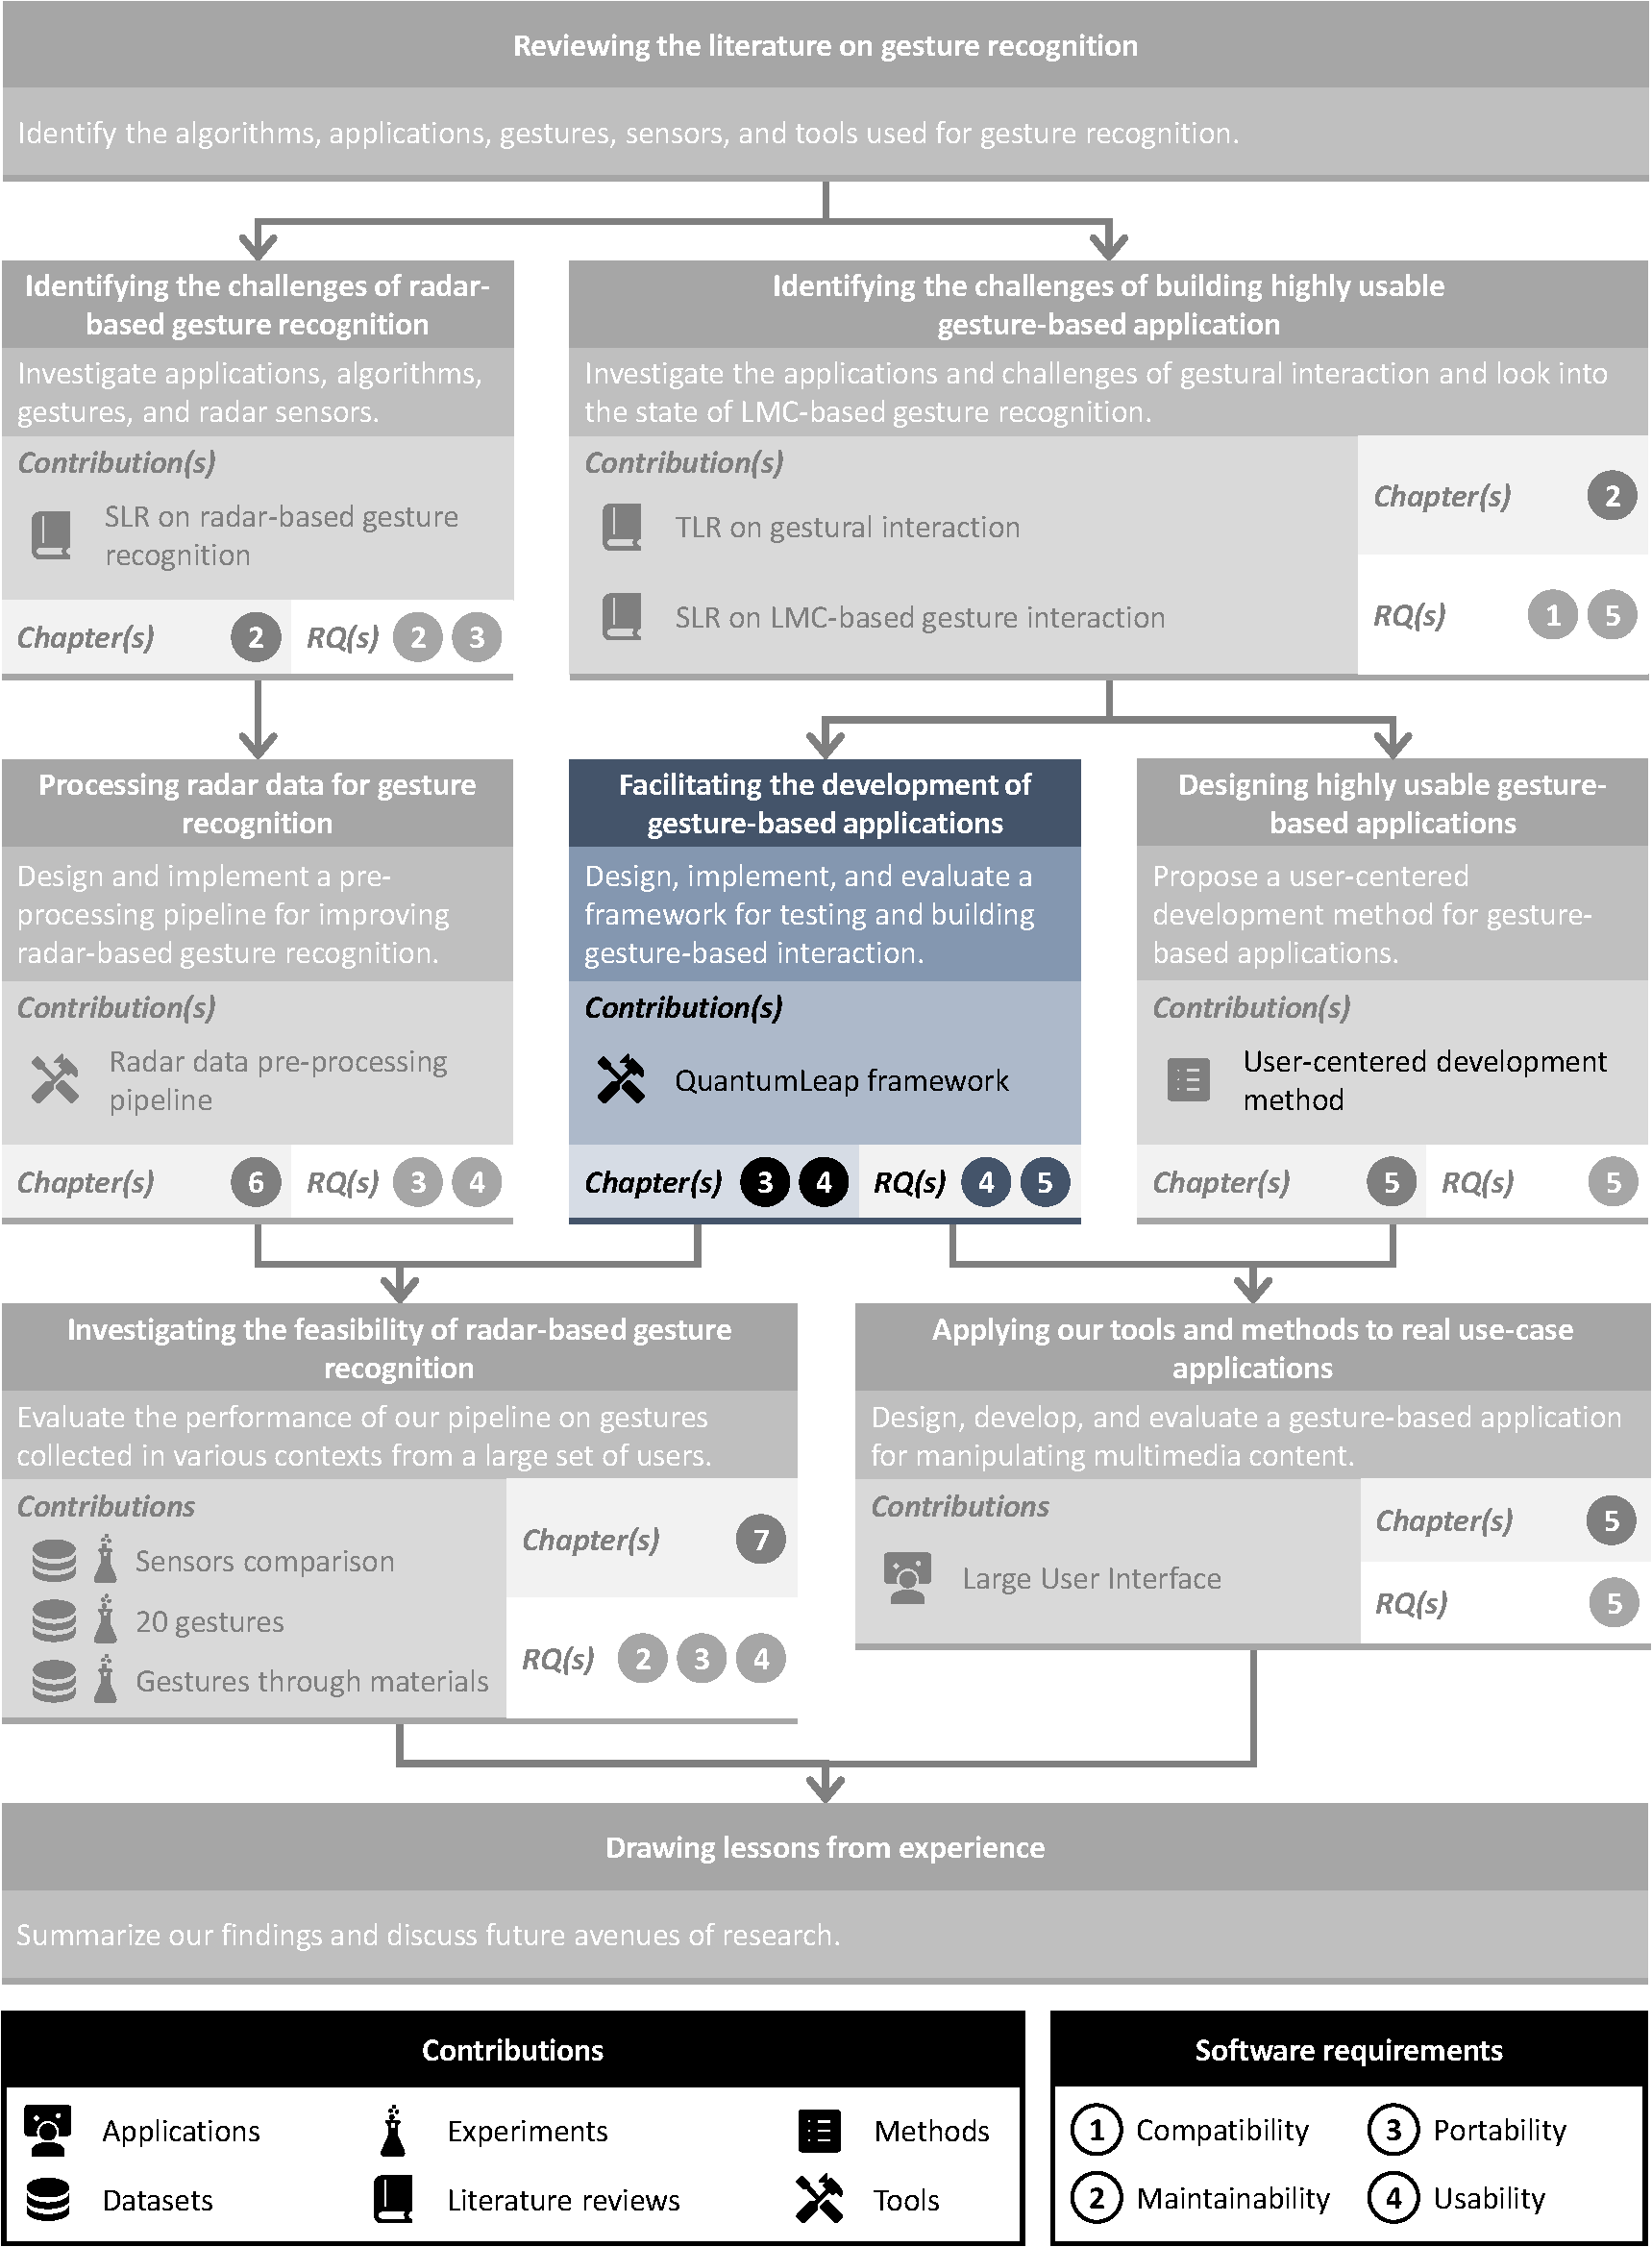
\includegraphics[width=\linewidth]{Figures/QuantumLeap/graphical-summary-quantumleap.pdf}
  \vspace{-18pt}
  \caption{Main contributions of this chapter.}
  \label{fig:quantumleap-testing:graphical-summary}
\end{figure}

The rest of this chapter is divided into three sections.
Section~\ref{sec:quantumleap-testing:description} first explains how the testing tool was integrated into \ql, its main features, and how it can be used to evaluate gesture recognition algorithms.
Section~\ref{sec:quantumleap-testing:discussion} then discusses its main advantages and limitations and Section~\ref{sec:quantumleap-testing:conclusion} concludes this chapter.

\paragraph{Resources.} The \ql testing tool is available on GitHub at \url{https://github.com/sluyters/QuantumLeap}.

%================================================================================%
\section{A Tool for Evaluating Gesture Recognition Algorithms} \label{sec:quantumleap-testing:description}
The \ql testing tool is based on the same architecture as the gesture recognition dataflow and is thus also written in JavaScript (ECMAScript 2019). The reuse of many \ql software components, from its backend to its frontend, vastly simplified its development and allowed this tool to work directly with all of the existing recognizer and dataset modules. \fig~\ref{fig:quantumleap-testing:archi} illustrates the testing tool architecture and data structures for inter-module communication are described in \tab~\ref{tbl:quantumleap:communication-data-structures}.
%
The rest of this section discusses the integration of this tool into \ql and the various testing procedures that it supports.

\begin{figure}[t]
  \centering
  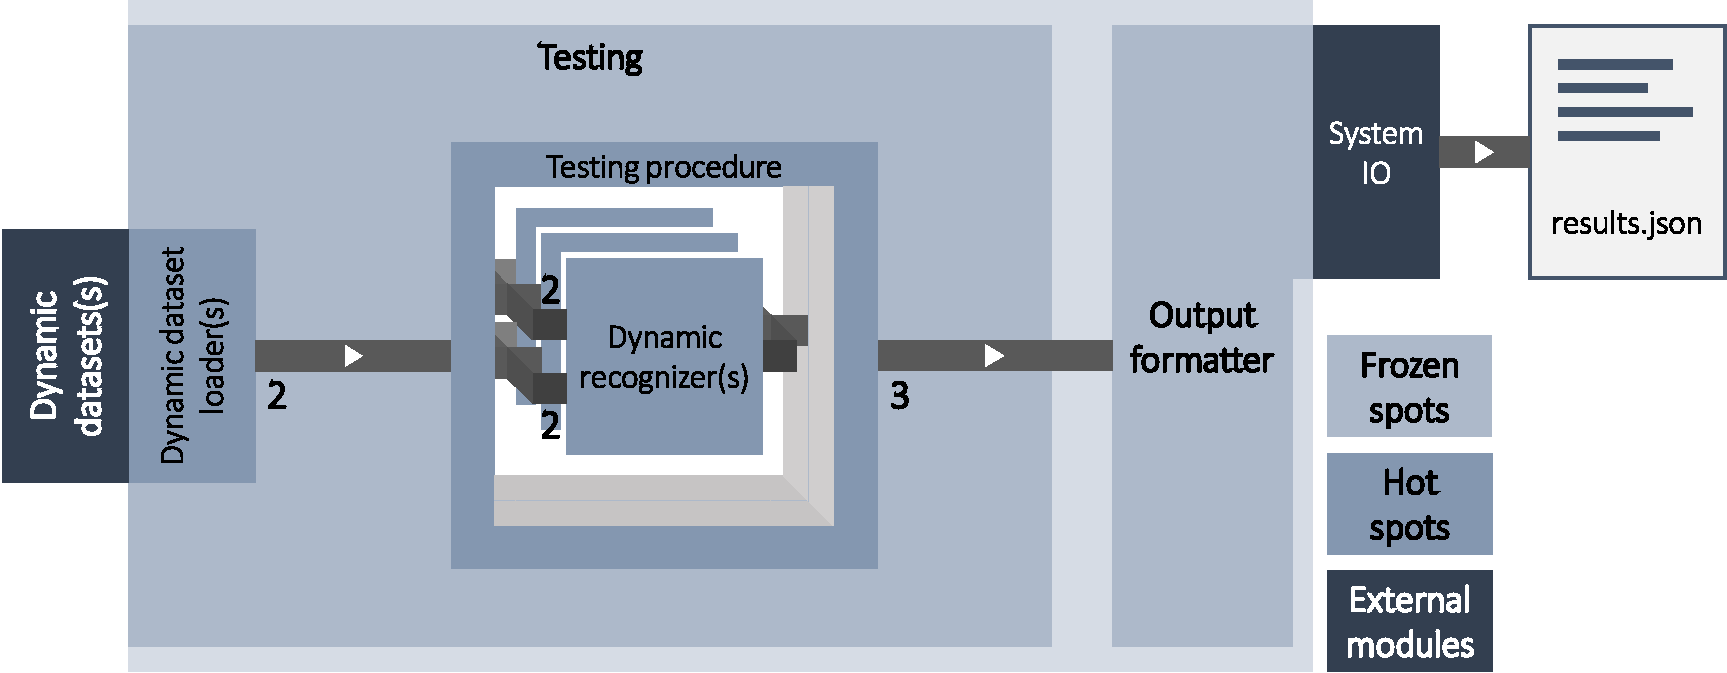
\includegraphics[width=\linewidth]{Figures/QuantumLeapTesting/quantumleap-testing.pdf}
  \vspace{-8pt}
  \caption{\ql testing tool architecture.}
  % \vspace{-8pt}
  \label{fig:quantumleap-testing:archi}
\end{figure}

%--------------------------------------------------------------------------------%
\subsection{Integration into \ql} \label{sec:quantumleap-testing:description:ql-integration}
\subsubsection{Modules} \label{sec:quantumleap-testing:description:ql-integration:modules}
This tool relies on the same dataset and recognizer modules as the \ql gesture recognition dataflow. However, it only supports the testing of static and dynamic recognizers. Testing other types of modules (\eg a segmenter) or combinations of modules (\eg a segmenter and a dynamic recognizer) would require modifications to its source code.

\subsubsection{Configuration} \label{sec:quantumleap-testing:description:ql-integration:configuration}

\begin{figure}[bt]
  \centering
  \begin{subfigure}{.49\textwidth}
      \centering
      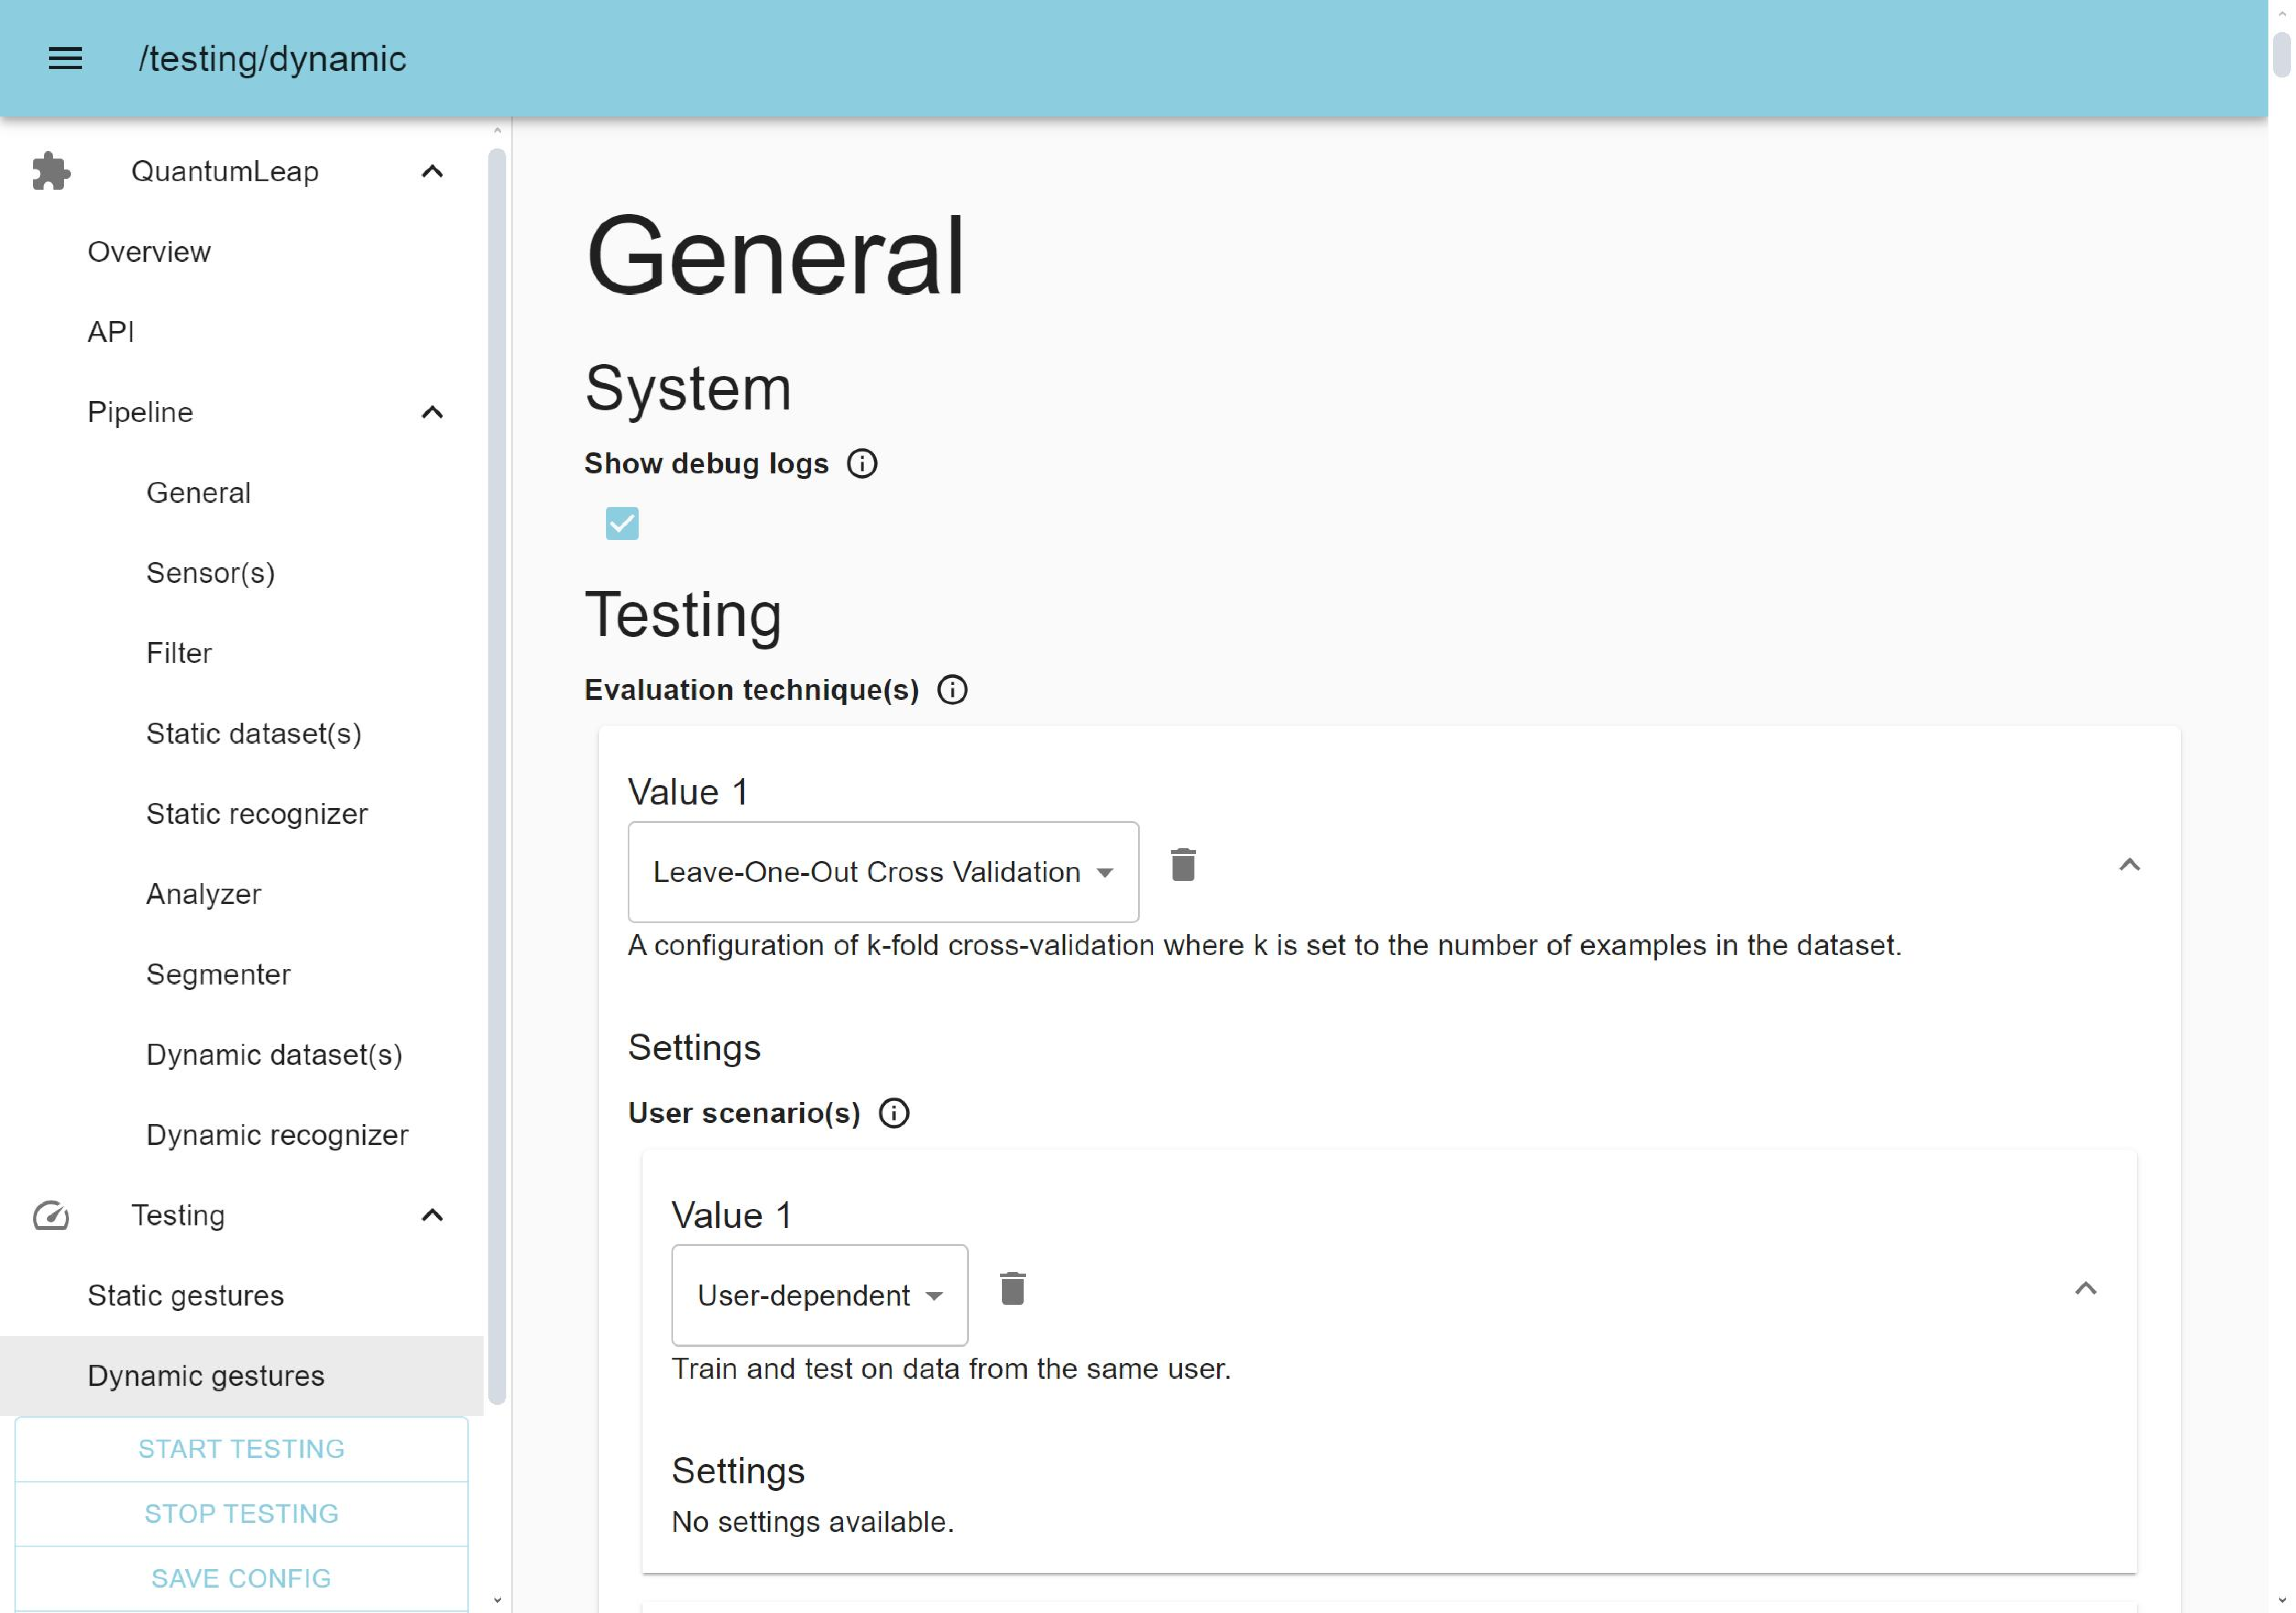
\includegraphics[width=\linewidth]{Figures/QuantumLeapTesting/QL-Testing-EvaluationTechnique.pdf}  
      \vspace{-15pt}
      \captionsetup{width=.9\linewidth}
      \caption{Evaluation techniques.}
      \label{fig:quantumleap-testing:ui:1}
  \end{subfigure}
  \begin{subfigure}{.49\textwidth}
      \centering
      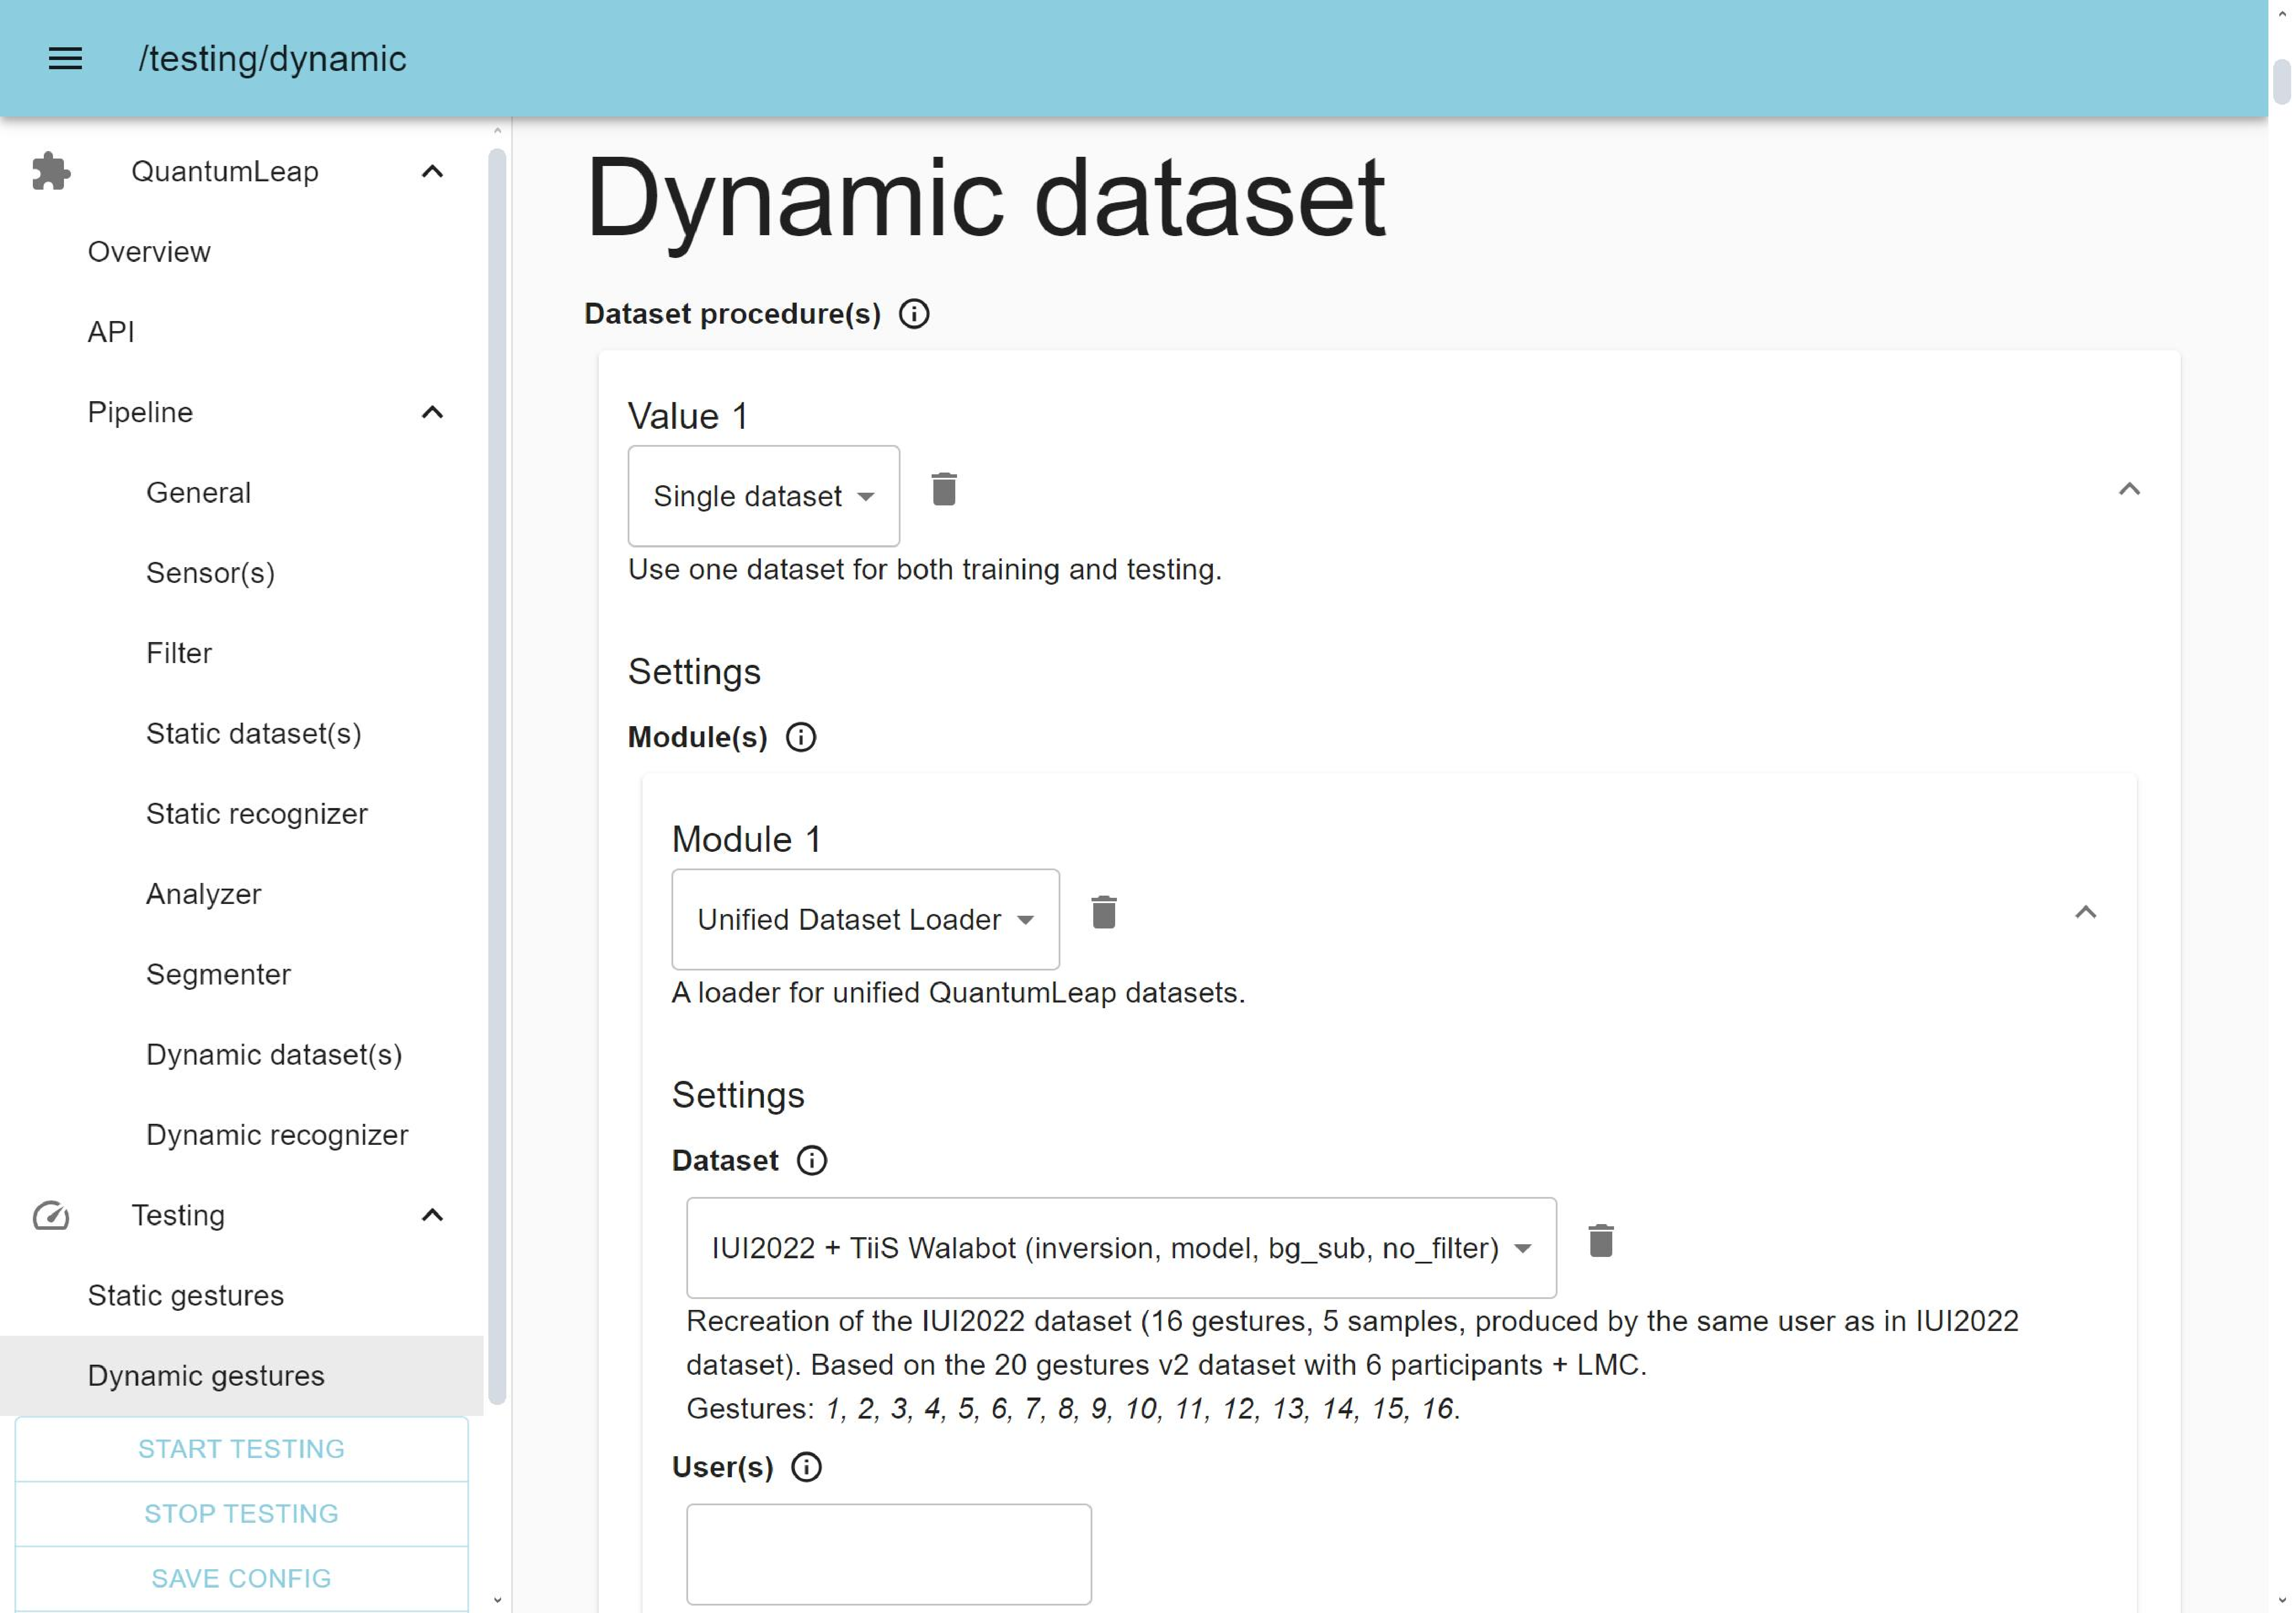
\includegraphics[width=\linewidth]{Figures/QuantumLeapTesting/QL-Testing-Dataset.pdf}  
      \vspace{-15pt}
      \captionsetup{width=.9\linewidth}
      \caption{Datasets.}
      \label{fig:quantumleap-testing:ui:2}
  \end{subfigure}
  
  \begin{subfigure}{.49\textwidth}
      \centering
      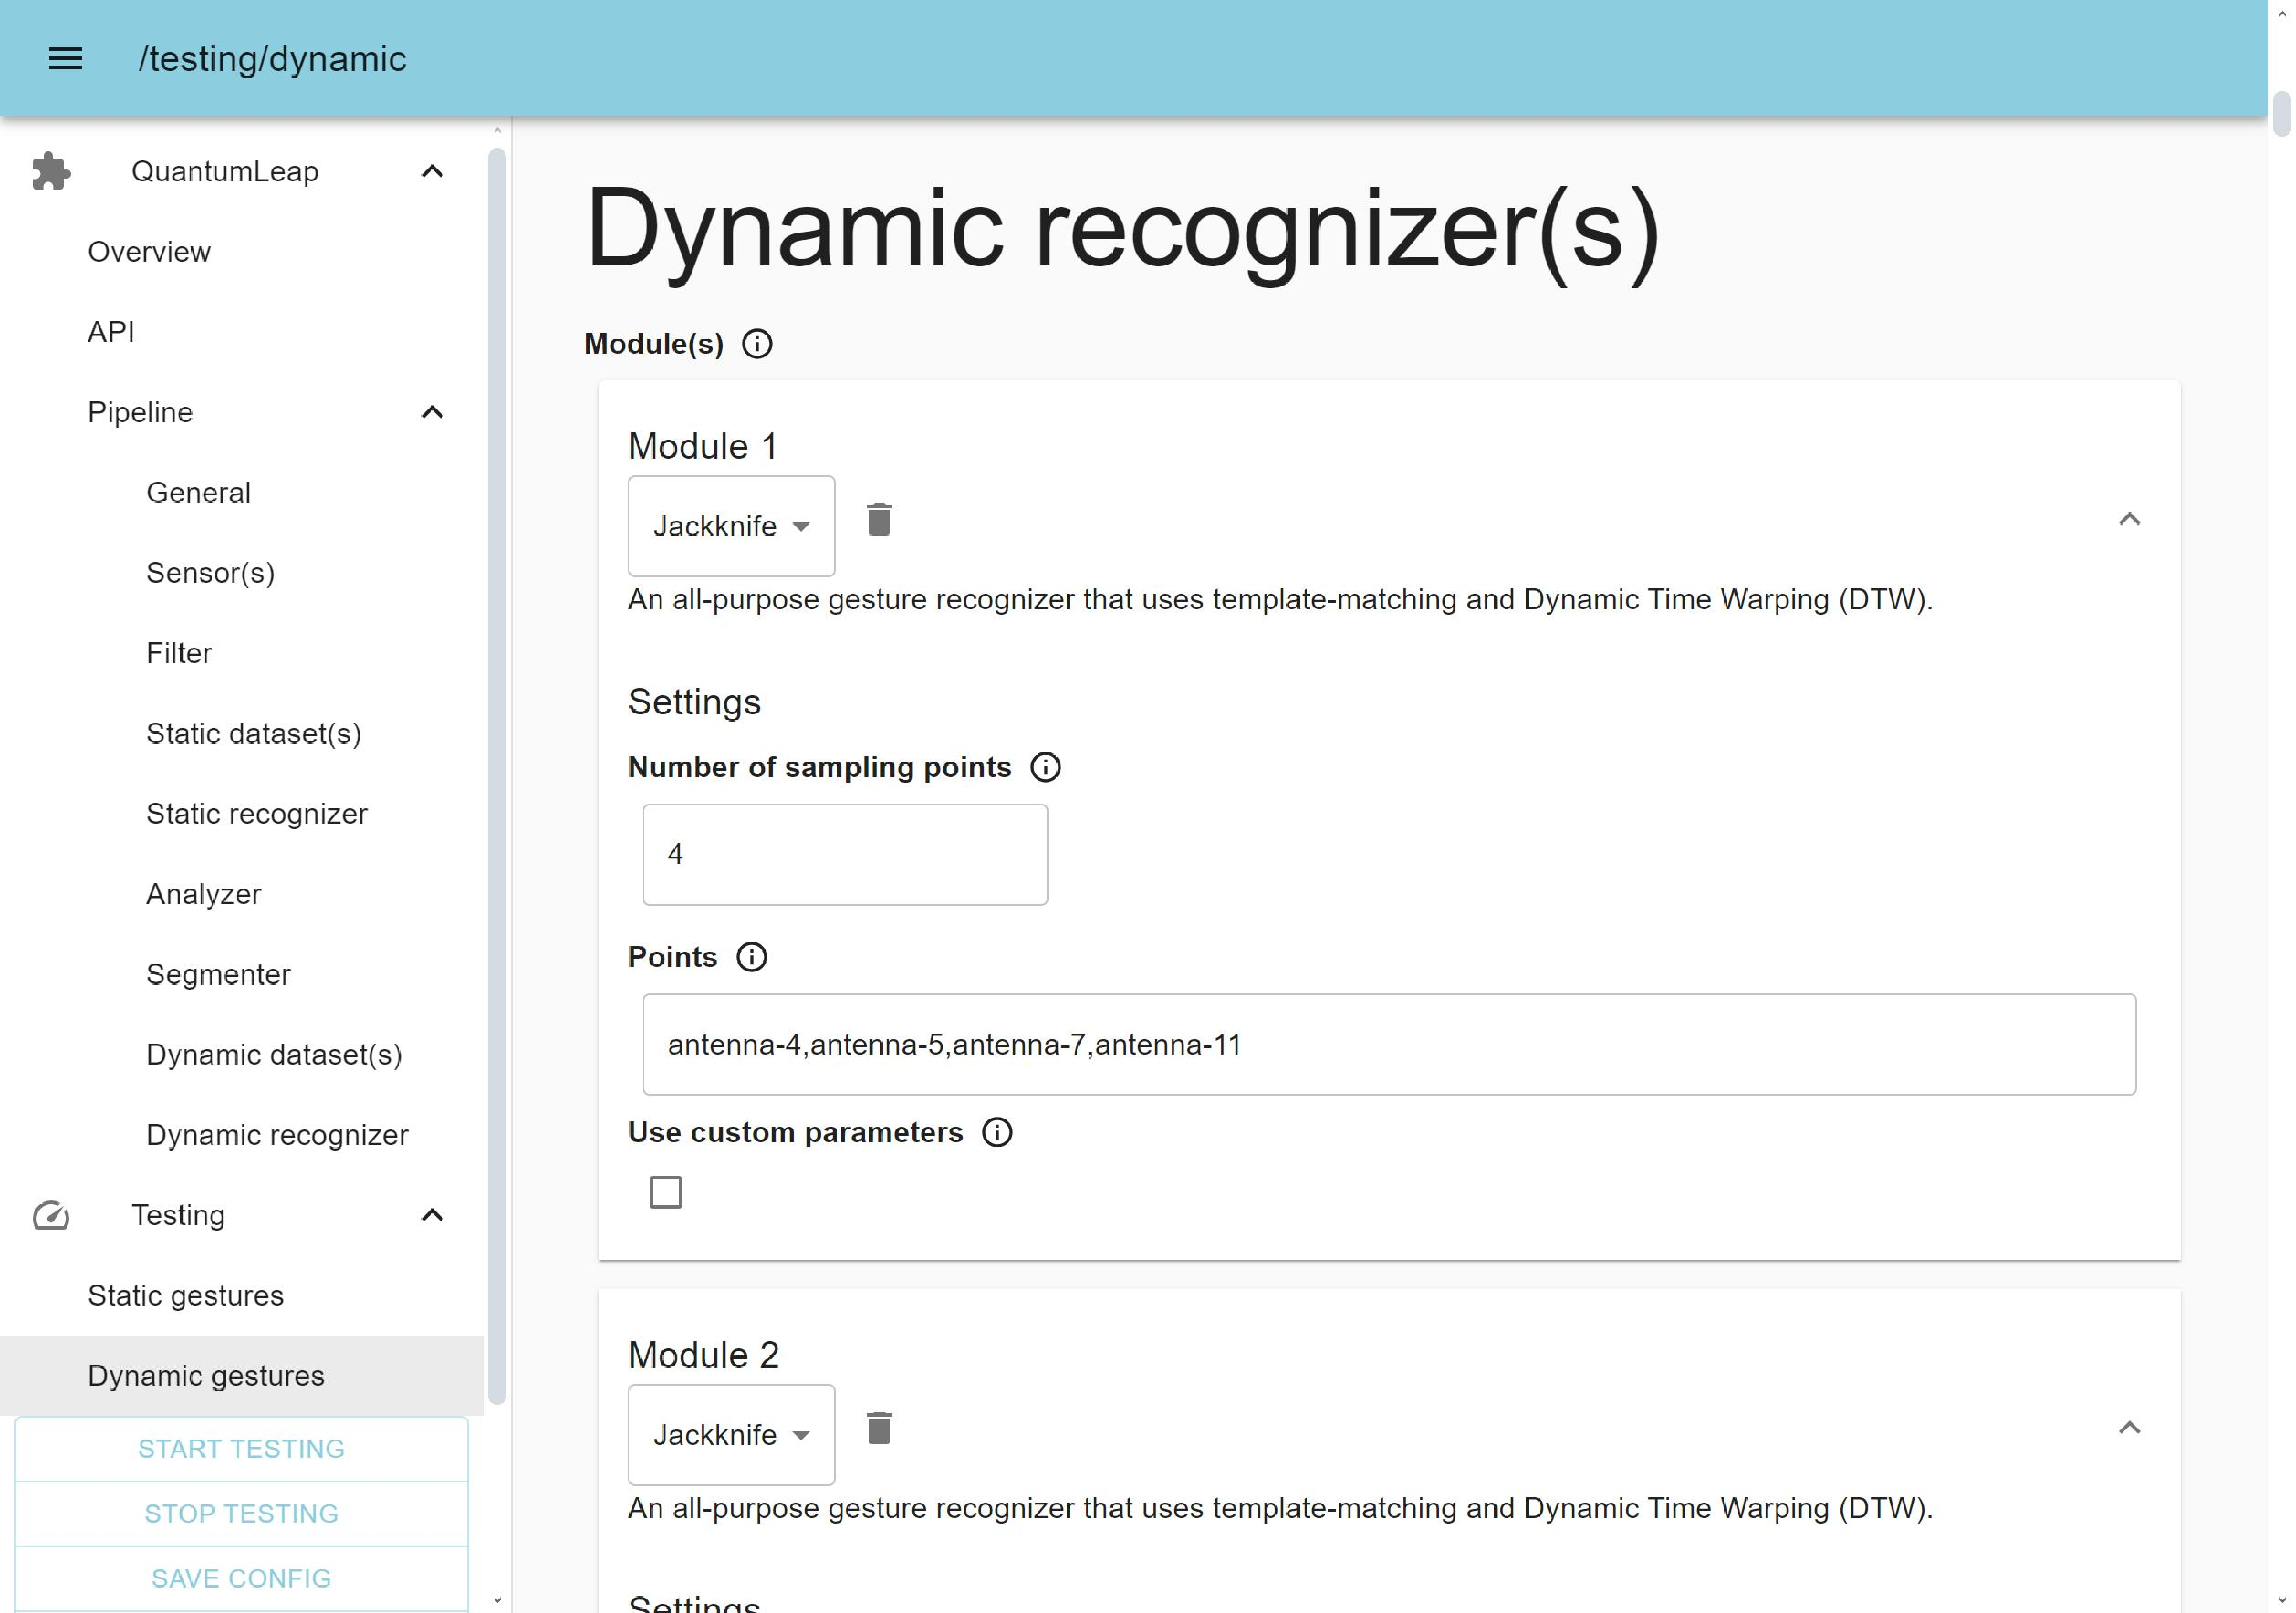
\includegraphics[width=\linewidth]{Figures/QuantumLeapTesting/QL-Testing-Recognizers.pdf}  
      \vspace{-15pt}
      \captionsetup{width=.9\linewidth}
      \caption{Recognizers.}
      \label{fig:quantumleap-testing:ui:3}
  \end{subfigure}

  % \vspace{-8pt}
  \caption{Screenshots of the \ql UI for testing.}
  \label{fig:quantumleap-testing:ui}
  % \vspace{-12pt}
\end{figure}

The testing configuration was integrated into the \ql configuration UI and features two pages: one for dynamic recognizers and another for static recognizers testing. For each type of recognizer, users can select and configure the evaluation technique(s), dataset(s), and recognizer(s) to test (\fig~\ref{fig:quantumleap-testing:ui}).
%
Testing parameters are displayed dynamically based on the ``config-template.json'' files of the testing and any selected module. Their assigned values are read from and saved to the ``config.json'' file of the testing. This file can be easily shared with, and modified by, other users so that they can attempt to reproduce or even replicate testing results. 
%
Buttons allow users to save the configuration and start the testing. The testing status (progress, time remaining), as well as potential warnings and errors, are displayed in the terminal. 

\subsubsection{Results} \label{sec:quantumleap-testing:description:ql-integration:results}
The \textit{recognition rate} (\ie the ratio of correctly recognized gestures divided by the number of trials) and the \textit{execution time} (\ie the time for recognizing the class of a candidate gesture) are computed for each tested recognizer configuration. In addition, individual trial results are summarized in a \textit{confusion matrix} (\ie a matrix representation of the predictions from the recognizer). 
Testing results are exported to JSON files, which can be parsed manually or with specialized tools to extract data and generate graphical representations. Each file features global testing parameters (\eg number of repetitions per gesture class, evaluation technique, dataset procedure) and aggregate results for each tested recognizer configuration (recognition rate, execution time, and confusion matrix). The format of the results is described below:

\begin{customcodeblock}[]{json}
[
  {
    "r": 100,
    "evaluationTechnique": "LOOCV"
    "datasetProcedure": "singleDataset|crossDataset",
    "userScenario": "userDependent"
    "datasets": [
      "Training dataset", 
      "Testing dataset (if crossDataset)"
    ],
    "gestures": ["Gesture 1", "Gesture 2"],
    "data": [
      {
        "name": "Name of the recognizer",
        "options": {
          "Option 1": "Value",
          "Option 2": "Value"
        },
        "data": [
          {
            "accuracy": 0.375,
            "time": 10.0,
            "confusionMatrix": [
              [50 50],
              [75 25]
            ]
          }
        ]
      }
    ]
  }
]
\end{customcodeblock}

%--------------------------------------------------------------------------------%
\subsection{Testing procedures} \label{sec:quantumleap-testing:description:testing-procedures}
\ql features ten different testing procedures for evaluating the performance of gesture recognizers. Support for new procedures may be added relatively easily in the future should the need arise. The ten currently supported procedures are listed in \tab~\ref{tab:quantumleap-testing:testing-procedures} along with a detailed description. 

\begin{table}
  \footnotesize
  \centering
  \begin{tabular}{lllp{6.9cm}}
      \toprule
      \textbf{Technique} & \textbf{Users} & \textbf{Dataset(s)} & \textbf{Procedure description}\newline For each combination of independent variables [...] \\
      \midrule
      TTS     & UD    & Single & For each gesture class in the dataset, repeat $R$ times: (1) select a random sample of that class for testing, (2) train the recognizer with $N$ samples per class randomly selected from the same user, and (3) attempt recognition.\\
                      \cmidrule{3-4}
              &       & Cross  & For each gesture class in the testing set, repeat $R$ times: (1) select a random sample of that class for testing, (2) train the recognizer with $N$ samples per class randomly selected from the same user in the training set, and (3) attempt recognition. \\
              \cmidrule{2-4}
              & UI    & Single & For each gesture class in the dataset, repeat $R$ times: (1) select a random sample of that class for testing, (2) train the recognizer with $N$ samples per class randomly selected from different users than the user of the testing samples, and (3) attempt recognition.\\
                      \cmidrule{3-4}
              &       & Cross  & For each gesture class in the testing set, repeat $R$ times: (1) select a random sample of that class for testing, (2) train the recognizer with $N$ samples per class randomly selected from different users than the user of the testing samples in the training set, and (3) attempt recognition.\\
      \midrule
      LOOCV   & UD    & Single & For each gesture sample in the dataset: (1) select the sample for testing, (2) use all other samples from the same user for training, and (3) attempt recognition. \\
                      \cmidrule{3-4}
              &       & Cross  & For each gesture sample in the testing set: (1) select the sample for testing, (2) train the recognizer with all samples in the training set from the same user, and (3) attempt recognition.\\
              \cmidrule{2-4}
              & UI    & Single & For each gesture sample in the dataset: (1) select the sample for testing, (2) train the recognizer with all other samples from other users, and (3) attempt recognition. \\
                      \cmidrule{3-4}
              &       & Cross  & For each gesture sample in the testing set: (1) select the sample for testing, (2) train the recognizer with all samples in the training set from other users, and (3) attempt recognition. \\
              \cmidrule{2-4}
              & Mixed & Single & For each gesture sample in the dataset: (1) select the sample for testing, 2) train the recognizer with all other samples, and (3) attempt recognition. \\
                      \cmidrule{3-4}
              &       & Cross & For each gesture sample in the testing dataset: (1) select the sample for testing, (2) train the recognizer with all samples in the training set, and (3) attempt recognition. \\
      \bottomrule
  \end{tabular}
  \caption{Testing procedures implemented in \ql.}
  \label{tab:quantumleap-testing:testing-procedures}
\end{table}

\subsubsection{Evaluation Techniques} \label{sec:quantumleap-testing:description:testing-procedures:evaluation-techniques}
\ql supports two evaluation techniques: 
(1) train-test split (TTS), in which testing and training samples are randomly selected from the dataset(s) and 
(2) leave-one-out cross-validation (LOOCV), an extreme case of k-fold cross-validation (with $k{=}1$) in which recognizers are systematically tested with each sample of the testing dataset while training with all other valid samples of the training dataset~\cite{Zhou:2019}.

\subsubsection{Dataset Procedures} \label{sec:quantumleap-testing:description:testing-procedures:dataset-procedures}
Two dataset procedures are also supported: (1) single-dataset, in which training and testing samples are selected from the same dataset, and (2) cross-dataset, where one dataset is used for training and the other for testing. 

\subsubsection{User Scenarios} \label{sec:quantumleap-testing:description:testing-procedures:user-scenarios}
Three user scenarios are supported by \ql: (1) user-dependent (UD), in which testing and training samples are produced by the same user~\cite{Vatavu:2013}, (2) user-independent (UI), in which the testing sample is produced by a different user than the training samples~\cite{Vatavu:2013}, and (3) mixed, in which testing and training samples may or may not be produced by the same user. The UD and UI scenarios are supported by both TTS and LOOCV, while only LOOCV supports the ``mixed'' scenario.


%================================================================================%
\section{Discussion} \label{sec:quantumleap-testing:discussion}
\subsection{Strengths} \label{sec:quantumleap-testing:discussion:strengths}
The \ql testing tool has multiple advantages over using custom, opportunistic scripts for evaluating gesture recognition algorithms.
%
It allows developers and practitioners to use the same modules in an evaluation and in a final application, which is more efficient and reduces the risk of errors when switching from testing to implementation.
%
It also proposes ten predefined evaluation protocols and saves the results in a standard format, that can be parsed to produce figures and extract relevant measures.
%
Its GUI enables users to select one or more modules to evaluate and configure them without having to modify their source code. Comparing the performance of multiple gesture recognizers in the same scenario thus becomes a painless and extremely efficient process.
%
Modules, testing configurations, and results can be shared with other researchers, providing them with all the necessary tools to attempt to repeat, replicate, and reproduce these results. By encouraging cooperation between researchers, this tool could foster the development of better algorithms for gesture recognition.

\subsection{Limitations} \label{sec:quantumleap-testing:discussion:limitations}
However, this testing tool suffers from a few limitations which could be addressed in the future.
%
For instance, evaluating a more complex gesture recognition pipeline (\eg a combination of filter, segmenter, and recognizer), while very relevant, is currently impossible without modifying the source code of the tool.
%
In addition, this tool is aimed at evaluating template-matching algorithms written in JavaScript. This currently limits its impact on the HCI community, although supporting more languages and other types of gesture recognition algorithms (\eg based on deep learning) may be possible in the future.
%
Finally, testing results are aggregated before being exported to a file, with no way to access individual trials. While these aggregated results may be easier to parse, they may not provide sufficient granularity for more in-depth analyses.

%================================================================================%
\section{Conclusion} \label{sec:quantumleap-testing:conclusion}
% Summary
In this chapter, we introduced the \ql testing tool, an extension of \ql (Chapter~\ref{chap:quantumleap}) that utilizes the same modules and datasets for evaluating the performance of gesture recognizers. It supports ten testing procedures and features standardized configuration files and results, allowing researchers to share all of the elements required to repeat, replicate, and reproduce their experiments.

% Software quality properties
Like \ql, this tool addresses the four software quality properties~\cite{iso25010} mentioned in Section~\ref{sec:introduction:research:research-questions}: compatibility, maintainability, portability, and usability.
%
As mentioned in Section~\ref{sec:quantumleap:conclusion}, \ql and its testing tool support the \textit{compatibility} property by relying on the same modules and datasets.
%
In terms of \textit{maintainability}, the \ql testing tool helps developers adapt their applications to different environments (sensor, gesture set), by making it easy to compare gesture recognizers and select the most suitable one for a specific environment.
%
Regarding \textit{portability}, \ql testing configurations, modules, and datasets can be shared by researchers so that other algorithms can be evaluated in the same conditions, thus contributing to the advancement of research on gesture recognition techniques. In addition, a testing procedure can be applied to many different modules in a matter of seconds without any modification to the source code.
%
With regards to \textit{usability}, the ability to evaluate and compare modules before employing them in an application enables developers to build more accurate gesture recognition, which can result in more usable applications.
%
Overall, our extensive use of the tool throughout the rest of this thesis highlights the benefits of designing software that satisfies these quality properties.

% Future works
Despite its advantages, the \ql testing tool still has limitations that could be addressed in future work.
%
One avenue for improvement involves supporting the evaluation of more complex gesture recognition dataflows, beyond gesture recognizers, such as combinations of filters, segmenters, and recognizers.
%
In addition, we could work on improving the granularity of the results output by the tool, to enable more in-depth analyses.
%
Finally, supporting other languages than JavaScript would vastly expand the possibilities of the tool, \eg by allowing researchers to evaluate deep learning algorithms written in Python or R.


\chapter{Designing Highly Usable Gesture-based Applications} \label{chap:lui}

Effective gesture-based interfaces should feature a concise set of gestures that are consistent across the application and align with user expectations, as hand gestures can be challenging to learn~\cite{Fruchard:2018}, produce~\cite{Vatavu:2013}, and remember~\cite{Nacenta:2013}. 
%
However, as we concluded in Section~\ref{sec:state_of_the_art:overview:summary}, designing such interfaces is a complex process that often confronts user preferences with the technical challenges of gesture recognition.
%
Active involvement of designers and end users throughout the whole development process is thus paramount to achieving an optimal outcome, \eg by collecting user preferences through GESs (Section~\ref{sec:state_of_the_art:overview:ges}) and by conducting usability evaluations.
%
In an attempt to lower the barriers to entry for the development of intuitive gestural interfaces, this chapter addresses one of the five research questions defined in Section~\ref{sec:introduction:research:research-questions}: 
\begin{itemize}
    \item [RQ5] \textit{How can tools and methods aid in designing gesture-based applications that operate independently of gesture recognition logic?}
\end{itemize}
To do so, we propose a user-centered iterative development method and evaluation protocol for gesture-based interfaces, which aims to support the development of highly usable gestural interfaces. We apply this method to \lui, a gesture-based application for browsing and manipulating multimedia content. 
%
\fig~\ref{fig:quantumleap-testing:graphical-summary} illustrates these contributions and how they fit within this thesis.

\begin{figure}
    \centering
    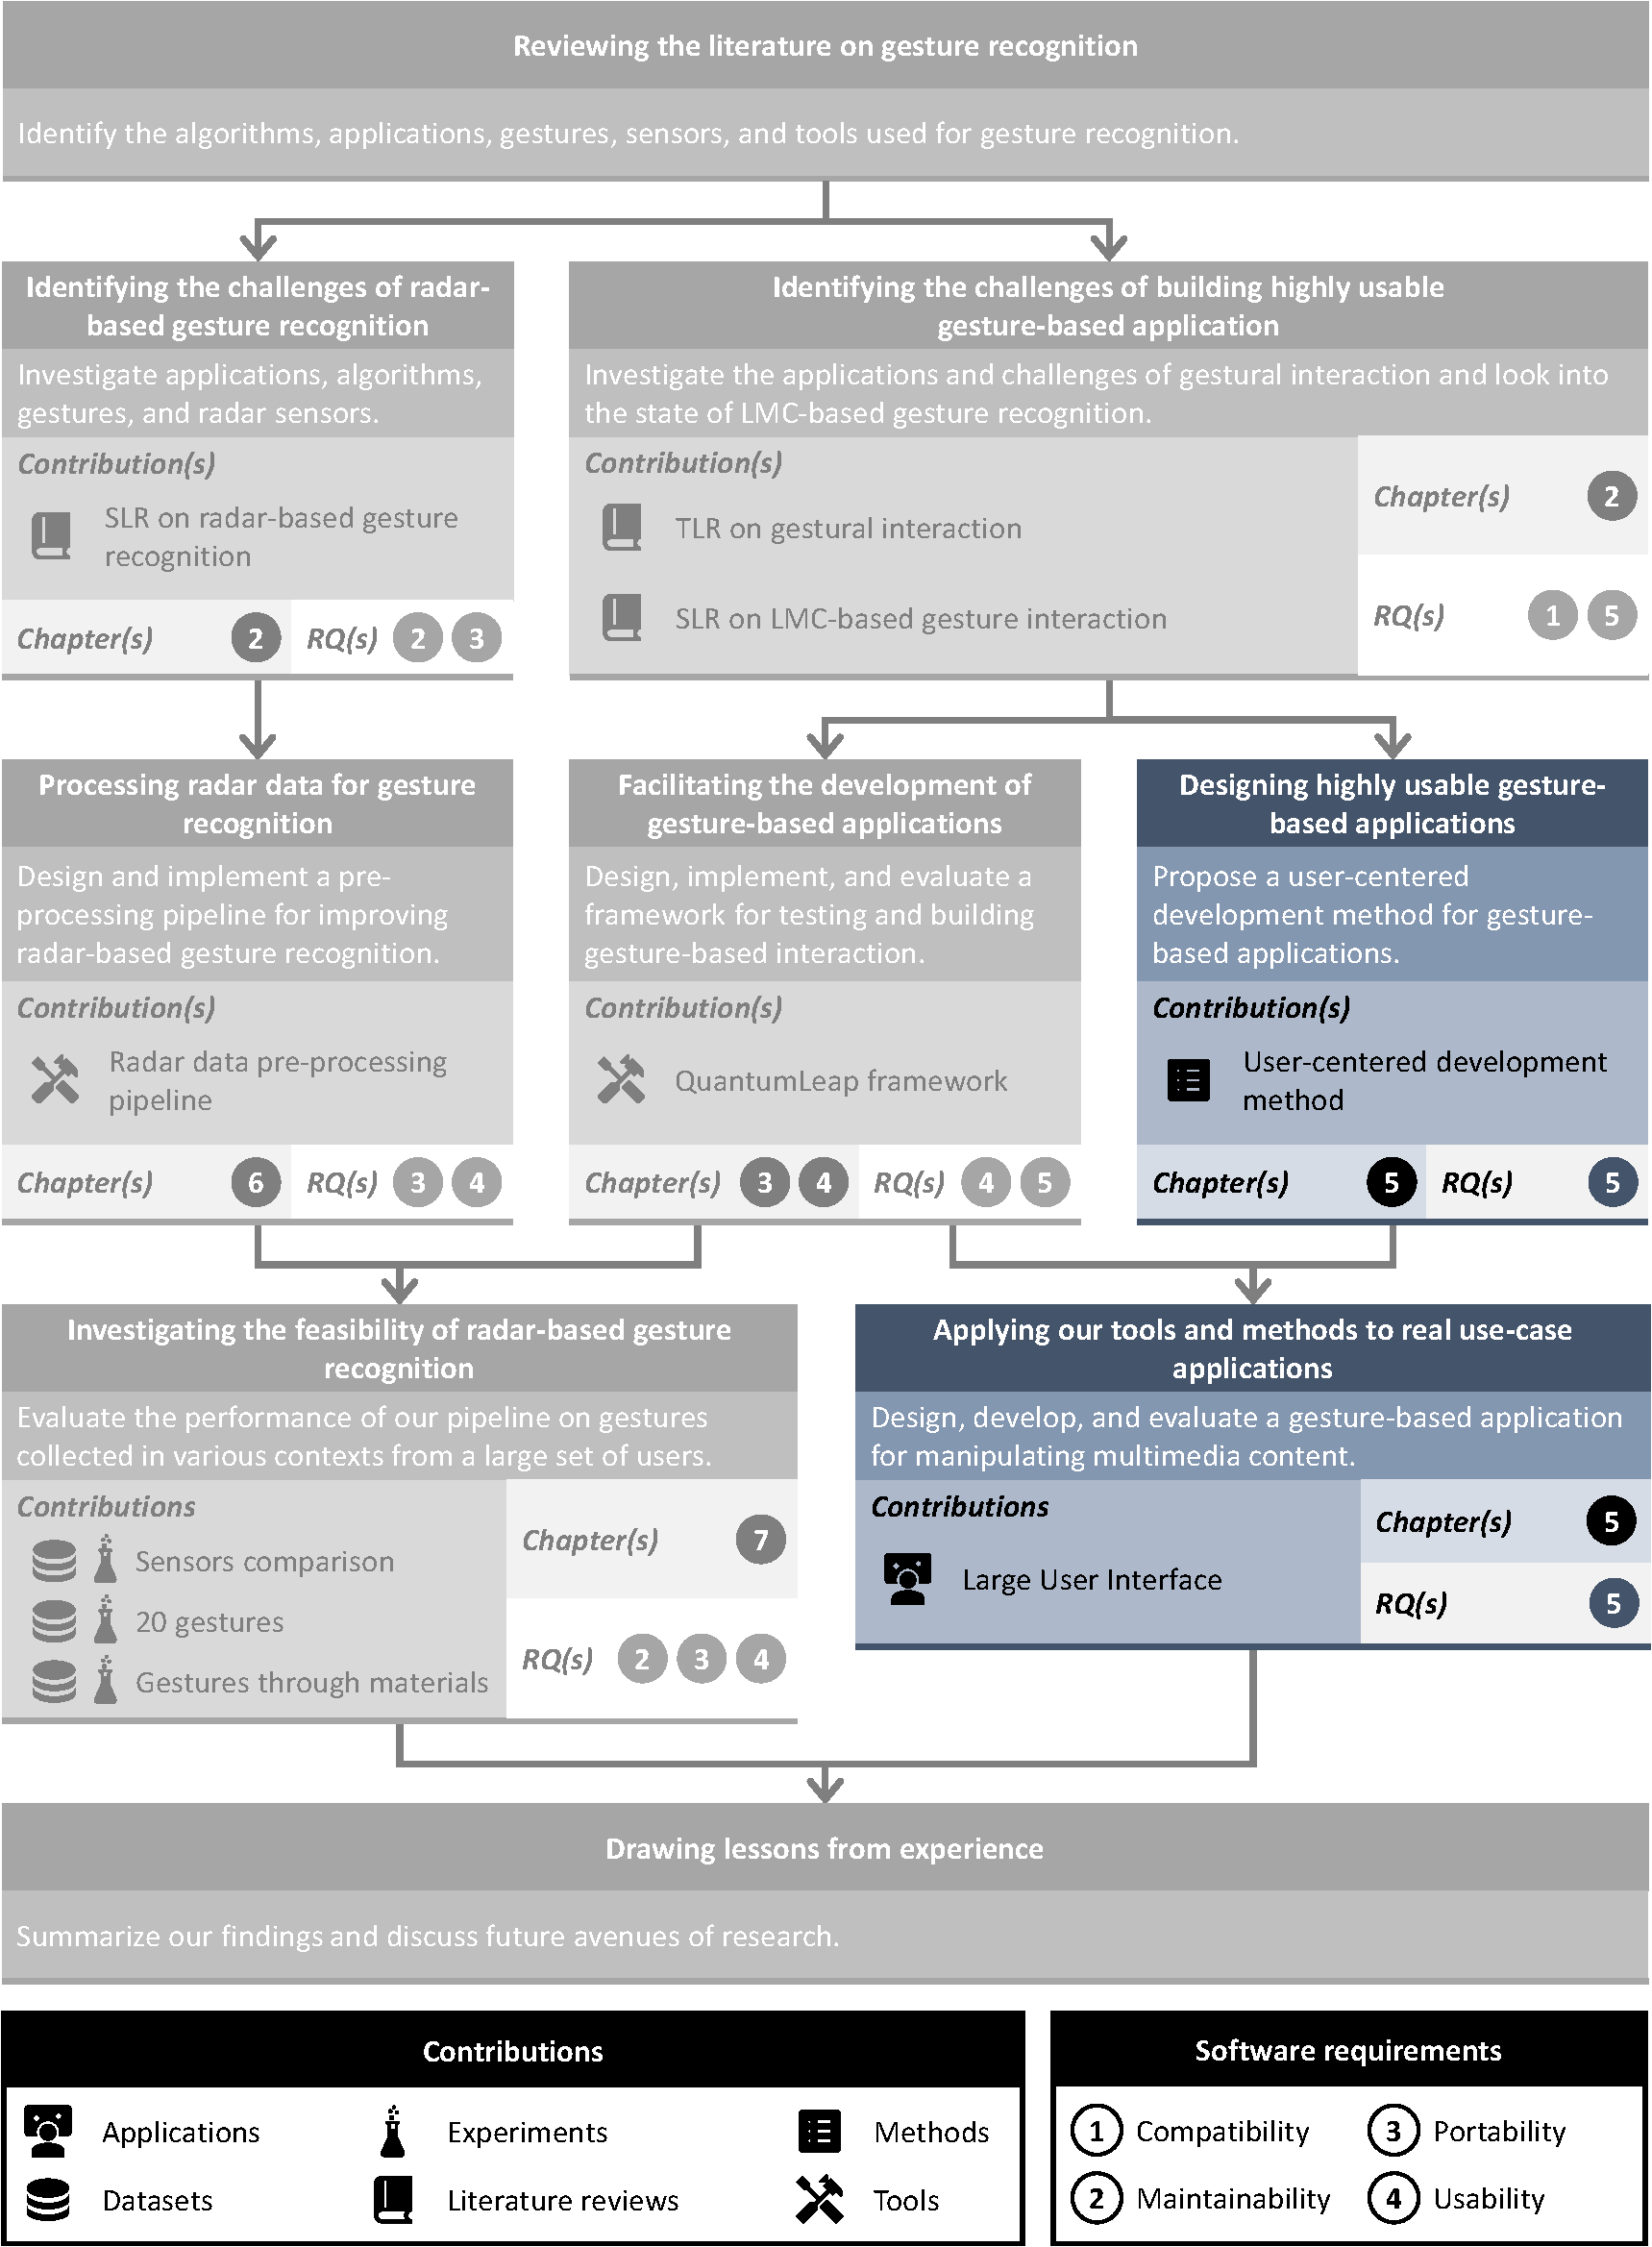
\includegraphics[width=\linewidth]{Figures/LUI/graphical-summary-large-user-interface.pdf}
    \vspace{-18pt}
    \caption{Main contributions of this chapter.}
    \label{fig:lui:graphical-summary}
\end{figure}

The rest of this chapter is organized as follows.
Section~\ref{sec:lui:description} first overviews the \lui application, its concepts, software architecture, and design requirements, and summarizes the differences between its three iterations.
Section~\ref{sec:lui:development-method} then details the stages of the development method used for \lui, including the design of a consistent gesture set, and the use of \ql for testing and implementing gesture interaction.
Section~\ref{sec:lui:evaluation} evaluates the overall quality of the interface, as well as the memorability and efficacy of the implemented gestures.
Finally, Section~\ref{sec:lui:discussion}  discusses the main strengths and limitations of \lui and Section~\ref{sec:lui:conclusion} concludes this chapter.

\paragraph{Publications.} This chapter is based on two papers published in the IJHCI journal~\cite{Sluyters:2022:LUI} and IJHCS journal~\cite{Sellier:2024}.

\paragraph{Resources.} The \lui application source code and its \ql configuration are available on GitHub at \url{https://github.com/sluyters/LUI}. Demonstration videos of \lui are available at \url{https://www.youtube.com/playlist?list=PLj1KcEqIa0fGRb0Z5E7f0UoL4LaxiKbm4}.

%================================================================================%
\section{The \lui Application} \label{sec:lui:description}

%--------------------------------------------------------------------------------%
\subsection{Overview} \label{sec:lui:description:overview}
\lui is a gesture-based interactive application for manipulating multimedia objects on large displays, such as TVs and wall displays, in a semi-public environment.
It currently focuses on interaction with photos, videos, documents, and maps, for which different sets of functions are desired (\tab~\ref{tab:lui:media-actions}). \lui is designed to be widely distributed and easily installed by being cheap to set up and easy to use. As such, we settled on using the Leap Motion Controller (LMC)\footnote{See \url{https://www.ultraleap.com/product/leap-motion-controller/}} for hand tracking, a cheap off-the-shelf sensor (less than 100\$) that can be plugged via USB to the computer. We selected the LMC for mid-air gesture interaction because it tracks two hands and their ten fingers~\cite{Colgan:2017} with high precision and robustness~\cite{Weichert:2013}, including the palm vector and hand radius. This sensor is comprised of two cameras and three infrared (IR) LEDs. The interaction space is .6m wide by .6m long by .6m deep, resulting in an .22 cubic meter volumetric space which takes the shape of an inverted pyramid above the sensor.
The LMC API~\cite{Spiegelmock:2013} enables to natively recognize a handful of system-defined gestures~\cite{Brandon:2014}, but custom gesture recognition algorithms often support a wider range of gestures~\cite{Bachmann:2018}. The LMC benefits from better accuracy and precision than other devices, such as an MS Kinect~\cite{Guzsvinecz:2019} or an Intel RealSense~\cite{Khalaf:2019}.
It is also widely used in many domains of applications such as augmented reality~\cite{Lopez:2015} and activity recognition~\cite{Marin:2016}. Several LMC-based gesture recognition algorithms exist~\cite{Bachmann:2018}. No study compares them on the same basis, apart from \cite{Filho:2018} with three classical machine learning algorithms, but without any recent recognizer such as DeepGru~\cite{Maghoumi:2019}.

\begin{table}
%    \vspace{-11pt}
    \footnotesize
    \centering
    \begin{tabular}{lcccc}
        \toprule
        \multicolumn{1}{c}{\multirow{2}{*}{\textbf{Function}}} & \multicolumn{4}{c}{\textbf{Media type}} \\
        & Photos & Videos & Documents & Maps \\
        \midrule
        Fullscreen on/off & \fullcirc & \fullcirc & \fullcirc & \fullcirc \\
        Like/dislike & \fullcirc & \fullcirc & \fullcirc & \fullcirc \\
        Previous/Next & \fullcirc & \fullcirc & \fullcirc & \emptycirc \\
        Zoom in/out & \fullcirc & \emptycirc & \fullcirc & \fullcirc \\
        Rotate & \fullcirc & \emptycirc & \fullcirc & \fullcirc \\
        Pan & \fullcirc & \emptycirc & \fullcirc & \fullcirc \\
        Change brightness & \fullcirc & \emptycirc & \emptycirc & \emptycirc \\
        Change contrast & \fullcirc & \emptycirc & \emptycirc & \emptycirc \\
        Play/pause & \emptycirc & \fullcirc & \emptycirc & \emptycirc \\
        Show/hide subtitles & \emptycirc & \fullcirc & \emptycirc & \emptycirc \\
        Volume up/down & \emptycirc & \fullcirc & \emptycirc & \emptycirc \\
        Fast-forward/backward & \emptycirc & \fullcirc & \emptycirc & \emptycirc \\
        Highlight text & \emptycirc & \emptycirc & \fullcirc & \emptycirc \\
        Place marker & \emptycirc & \emptycirc & \emptycirc & \fullcirc \\
        Change layer & \emptycirc & \emptycirc & \emptycirc & \fullcirc \\
        \bottomrule
    \end{tabular}
    \vspace{-4pt}
    \caption{List of functions for each media type.}
    % \vspace{-10pt}
    \label{tab:lui:media-actions}
\end{table}

\begin{figure}[p]
    \centering
    % \vspace{-10pt}
    \begin{subfigure}{.47\textwidth}
        \centering
        
\includegraphics[width=.96\linewidth]{Figures/LUI/UI/welcome_screen_lui.pdf}  
        \vspace{-5pt}
        \captionsetup{width=.9\linewidth}
        \caption{Welcome screen.}
        \label{fig:lui:screenshots:welcome-screen}
    \end{subfigure}
    \begin{subfigure}{.47\textwidth}
        \centering
        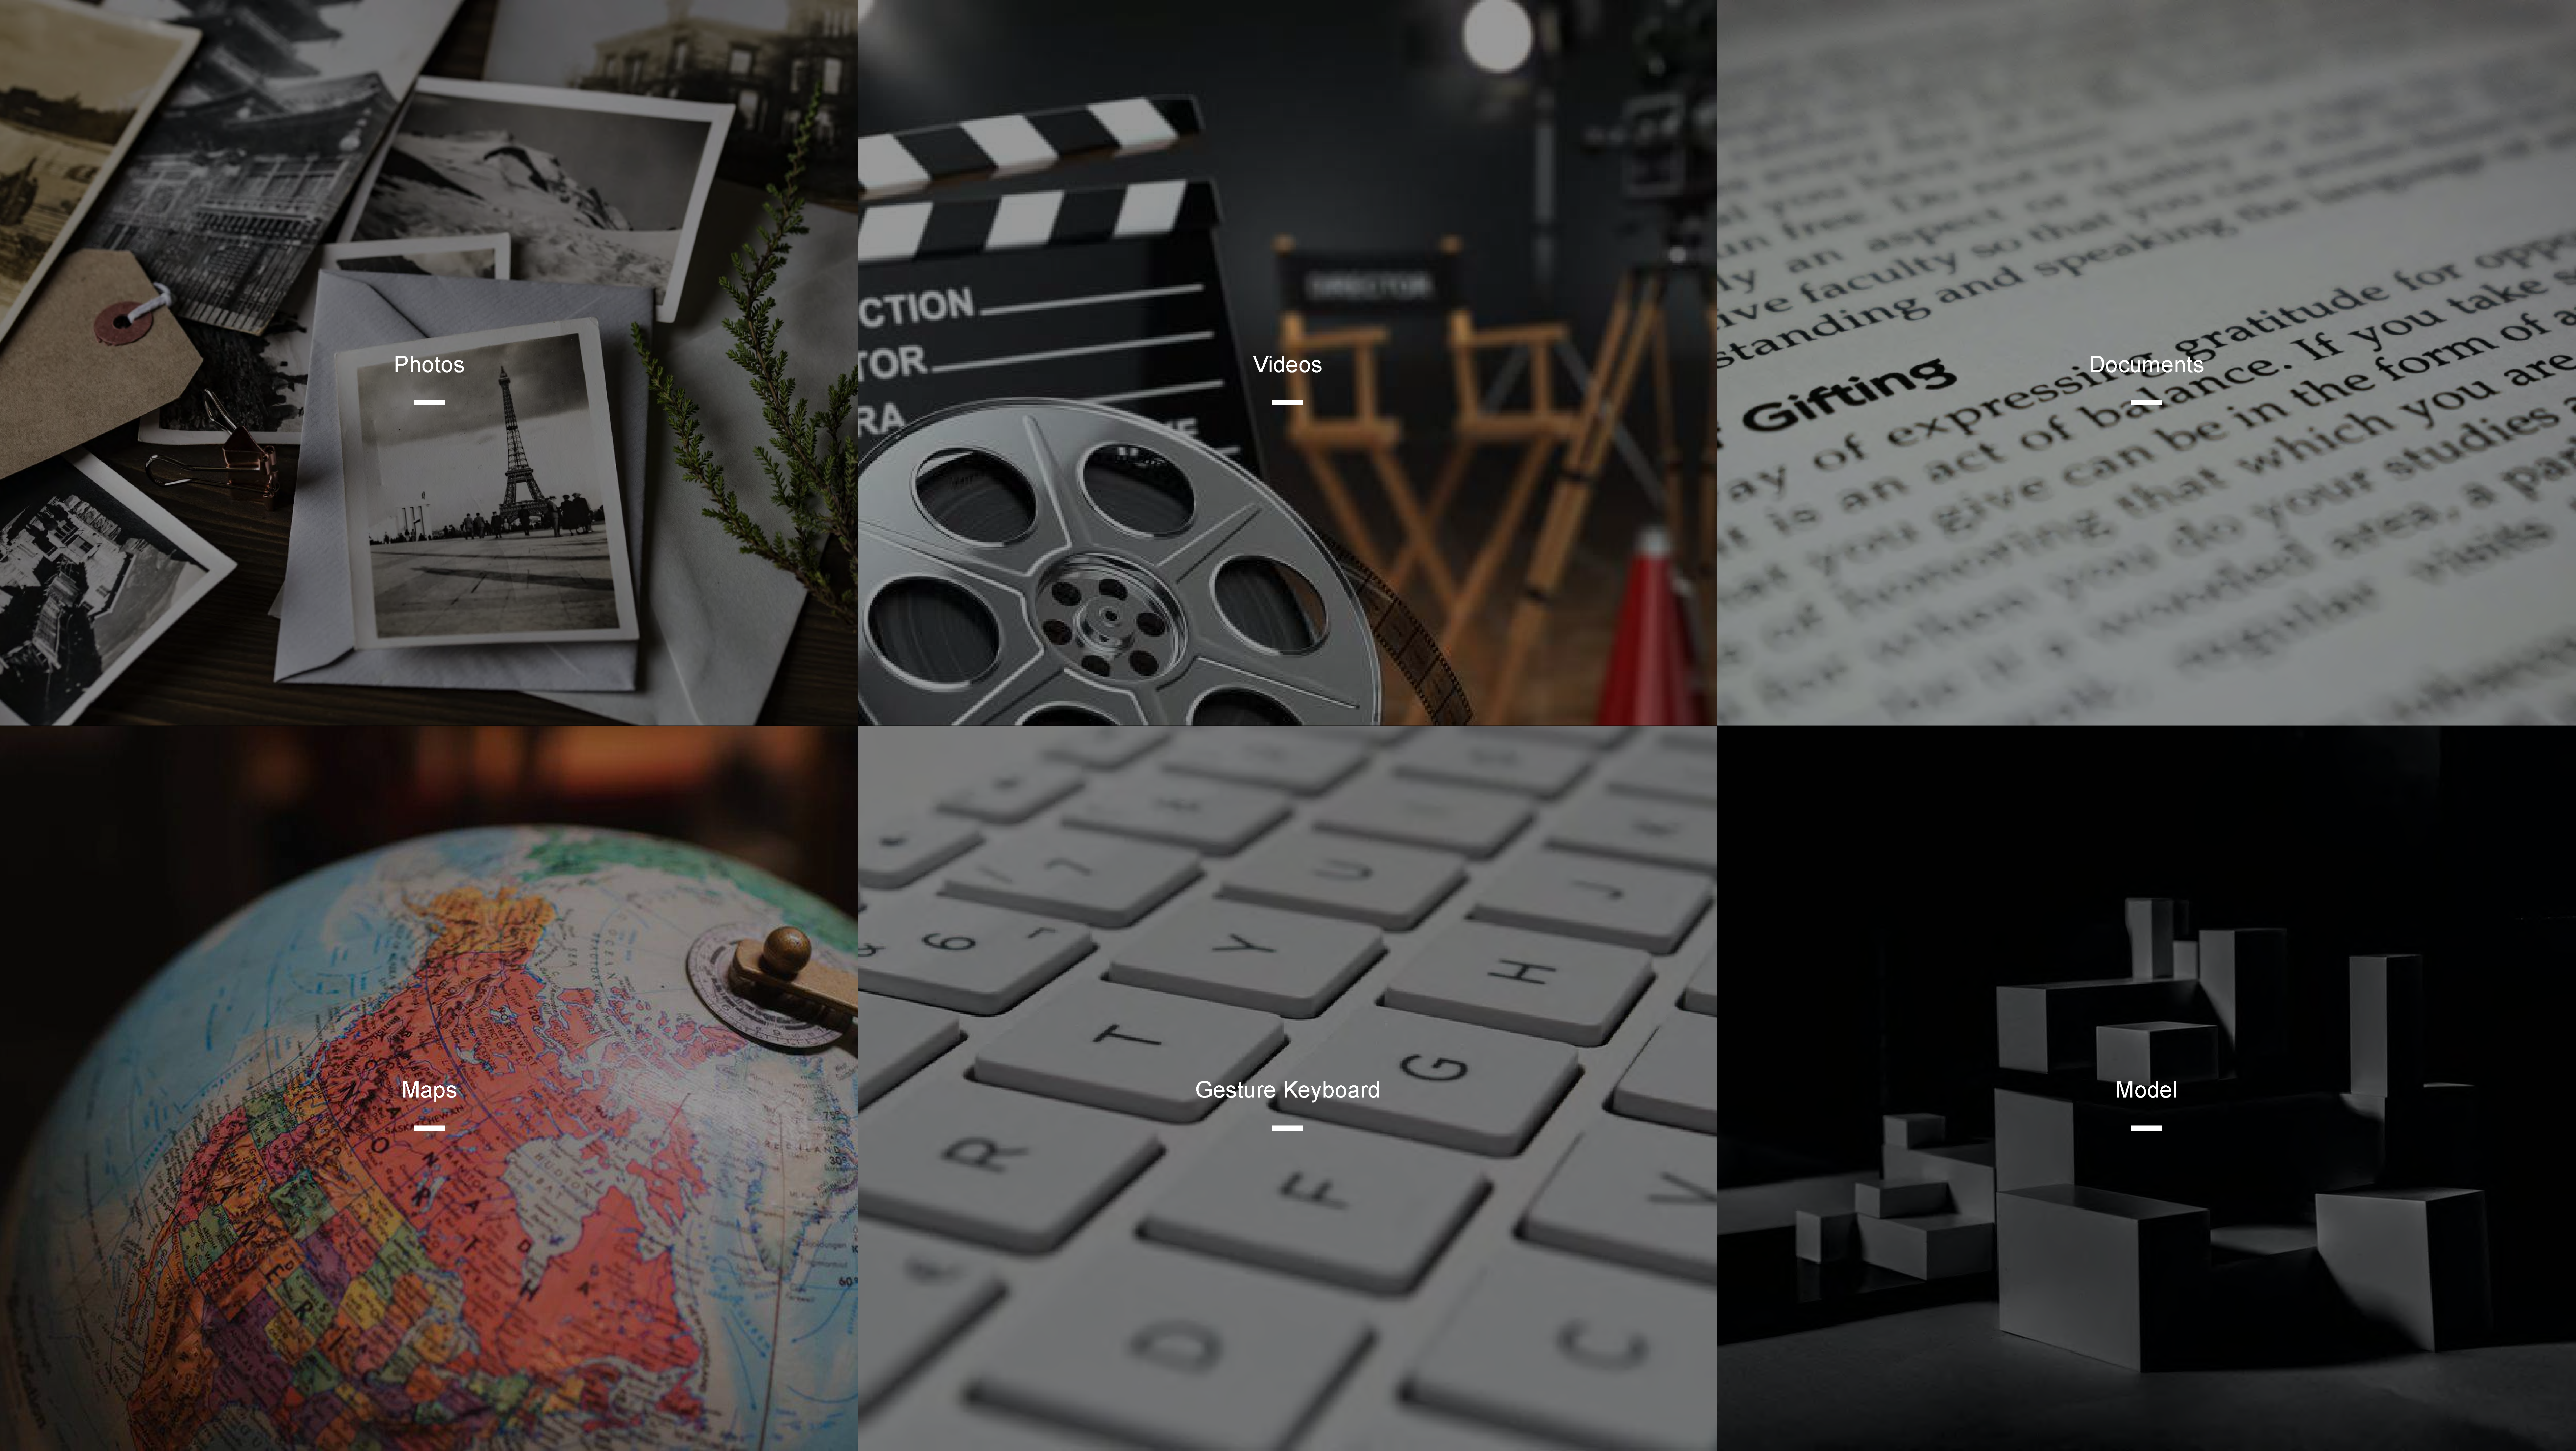
\includegraphics[width=.96\linewidth]{Figures/LUI/UI/app_menu.pdf}  
        \vspace{-5pt}
        \captionsetup{width=.9\linewidth}
        \caption{Application menu.}
        \label{fig:lui:screenshots:app-menu}
    \end{subfigure}

    \begin{subfigure}{.47\textwidth}
        \centering
        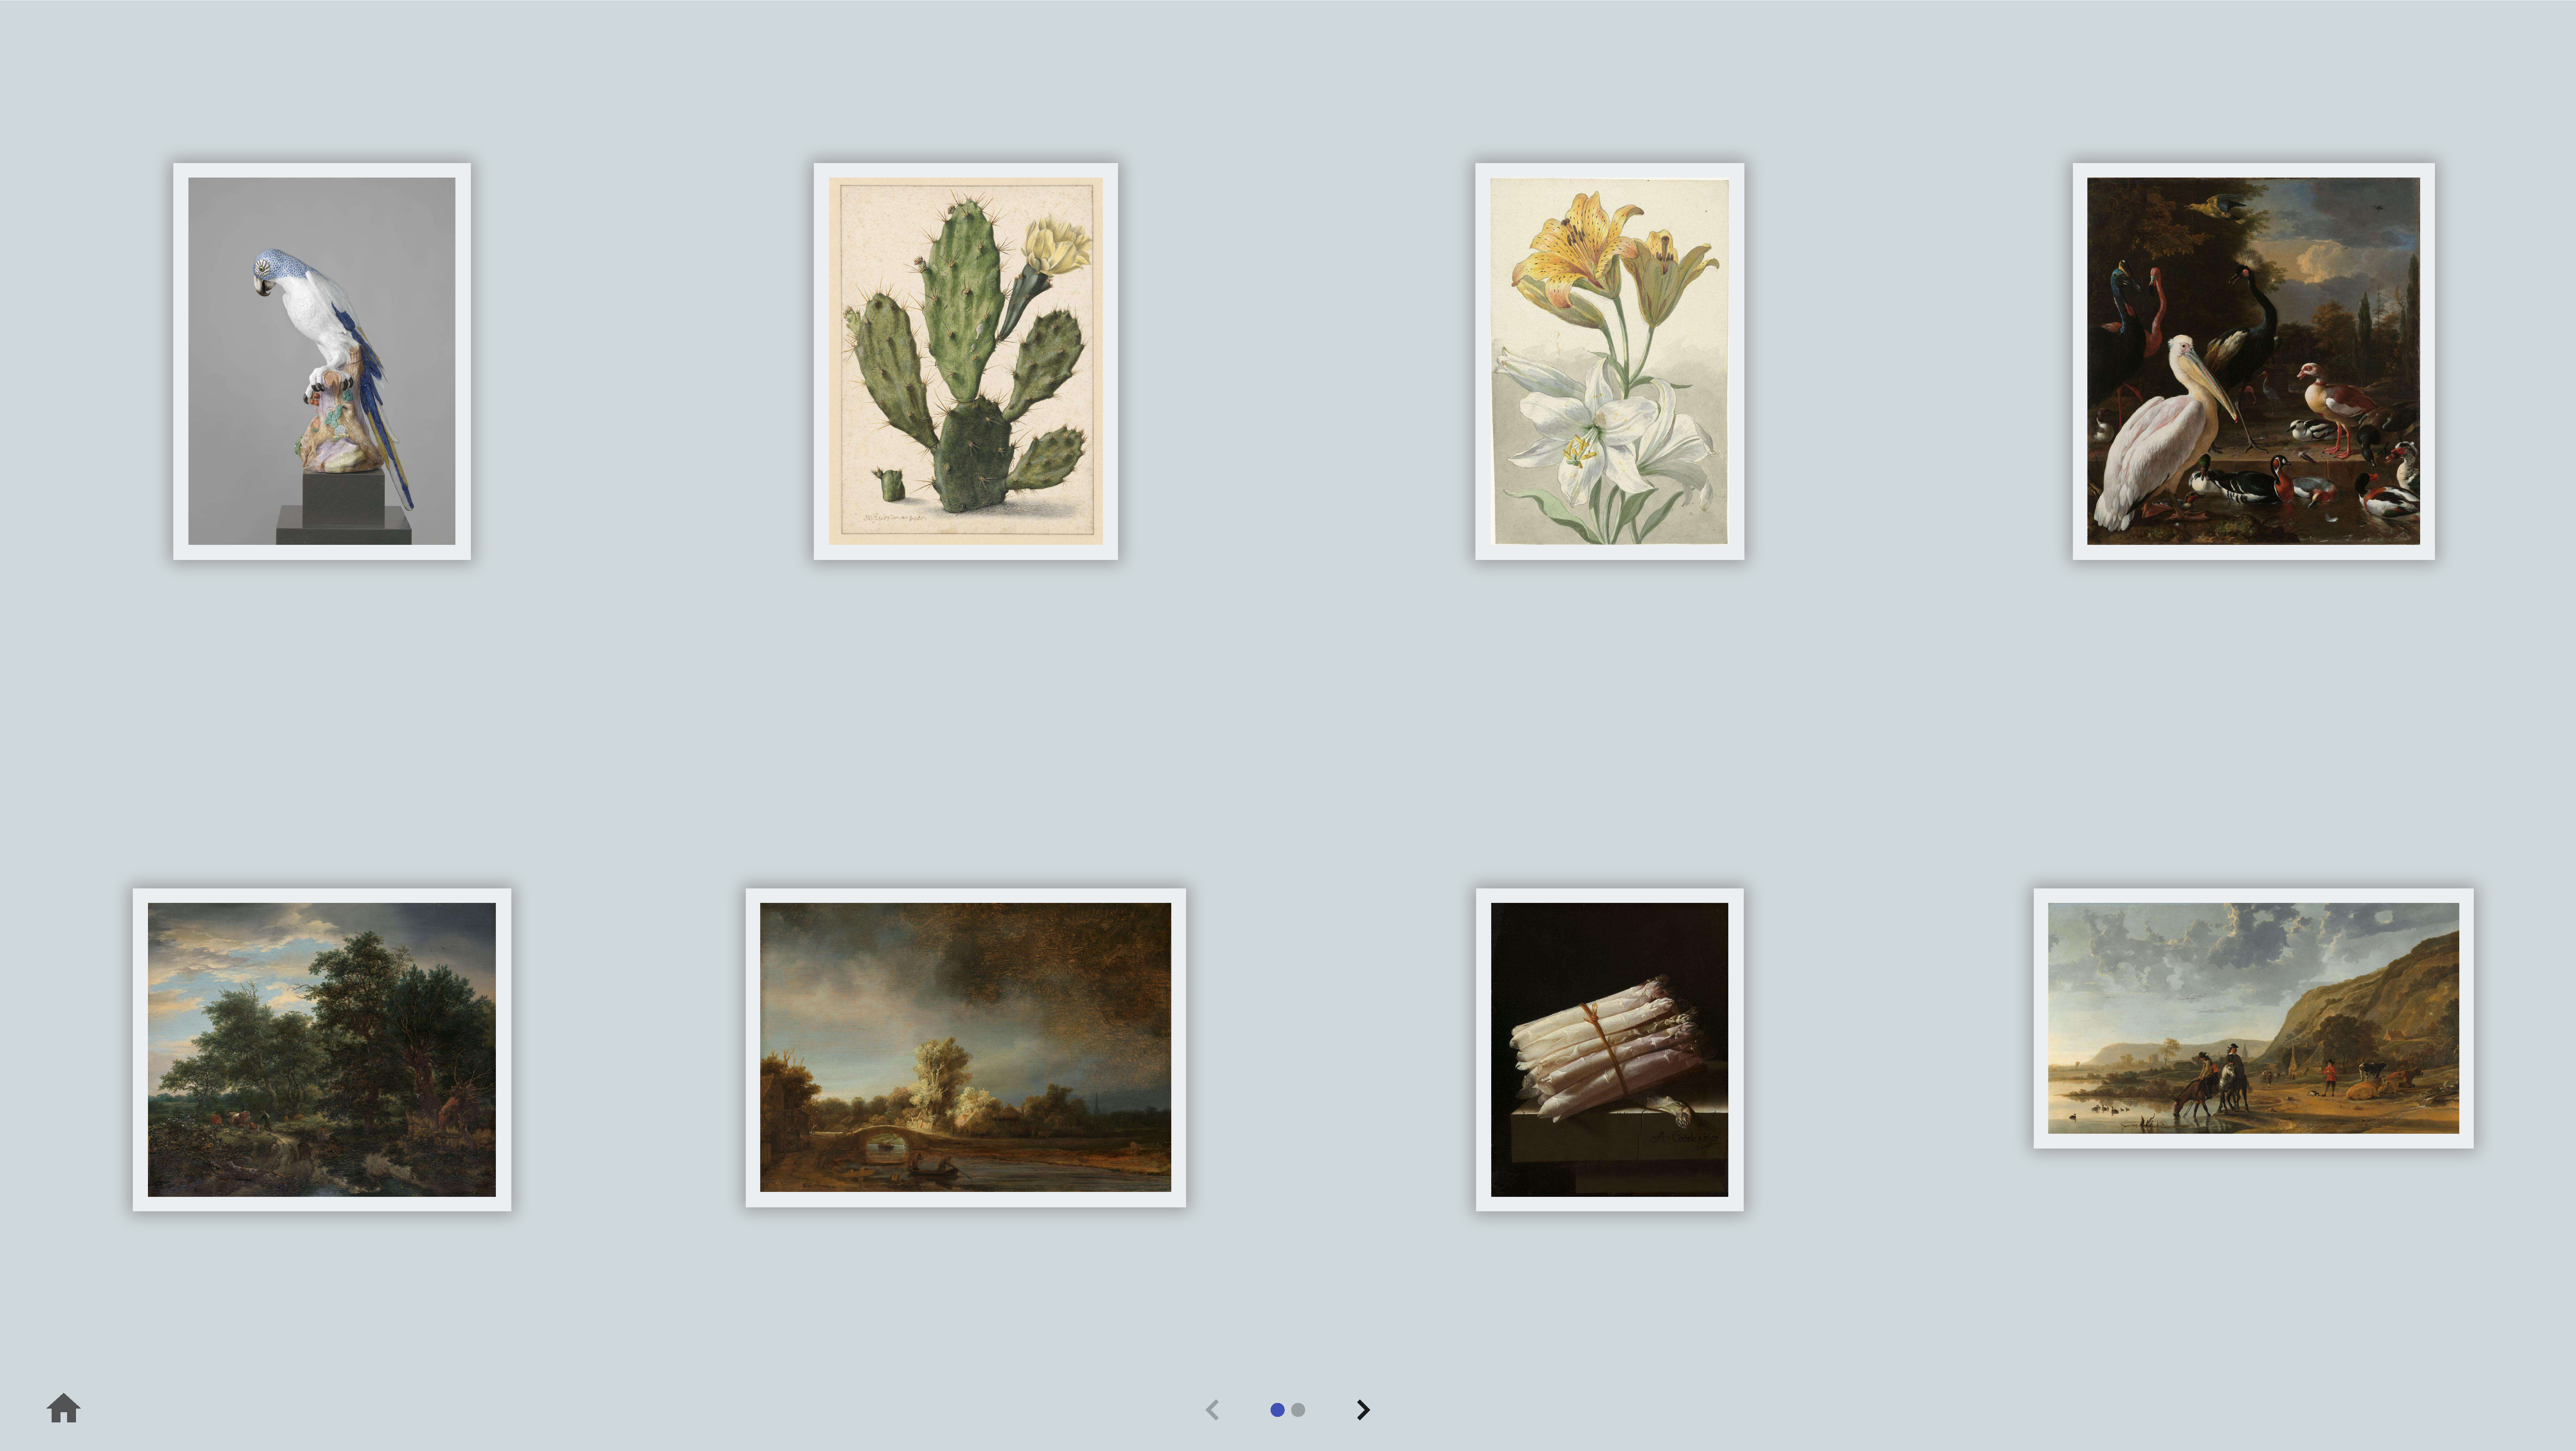
\includegraphics[width=.96\linewidth]{Figures/LUI/UI/photos-list.pdf}  
        \vspace{-5pt}
        \captionsetup{width=.9\linewidth}
        \caption{Photos app (list).}
        \label{fig:lui:screenshots:photos-list}
    \end{subfigure}
    \begin{subfigure}{.47\textwidth}
        \centering
        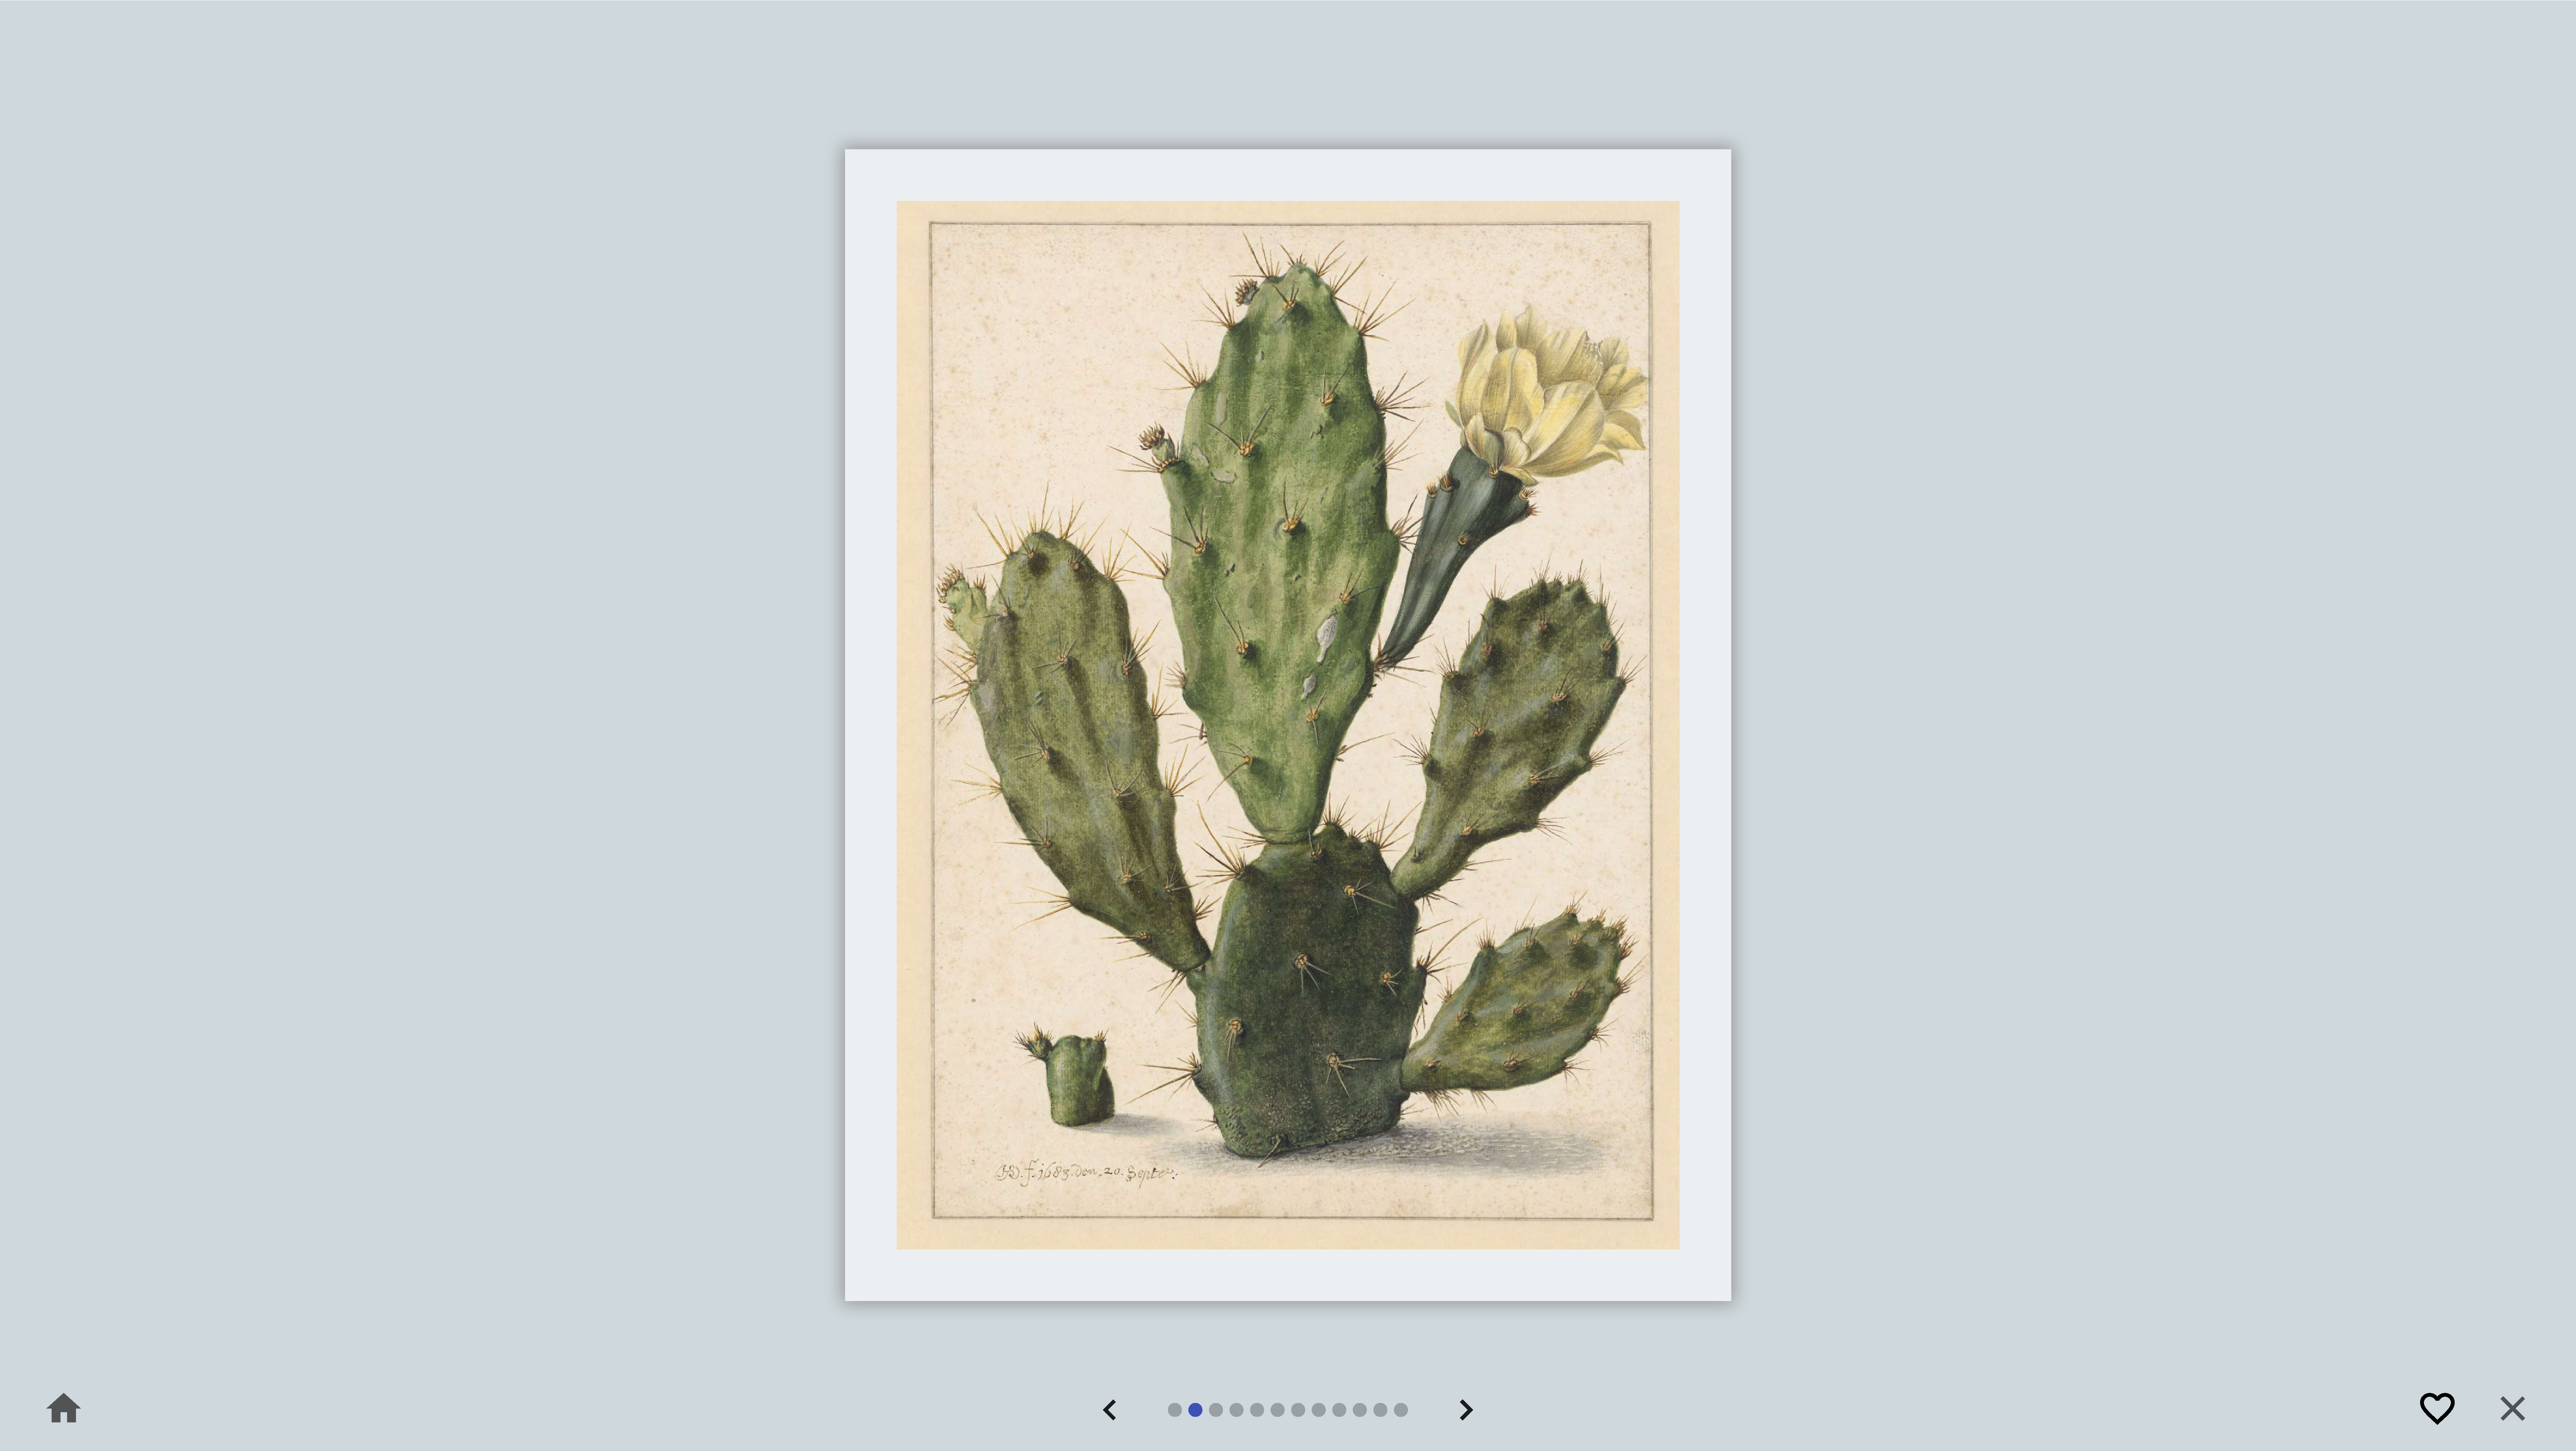
\includegraphics[width=.96\linewidth]{Figures/LUI/UI/photos-fullscreen.pdf}  
        \vspace{-5pt}
        \captionsetup{width=.9\linewidth}
        \caption{Photos app (item).}
        \label{fig:lui:screenshots:photos-fullscreen}
    \end{subfigure}

    \begin{subfigure}{.47\textwidth}
        \centering
        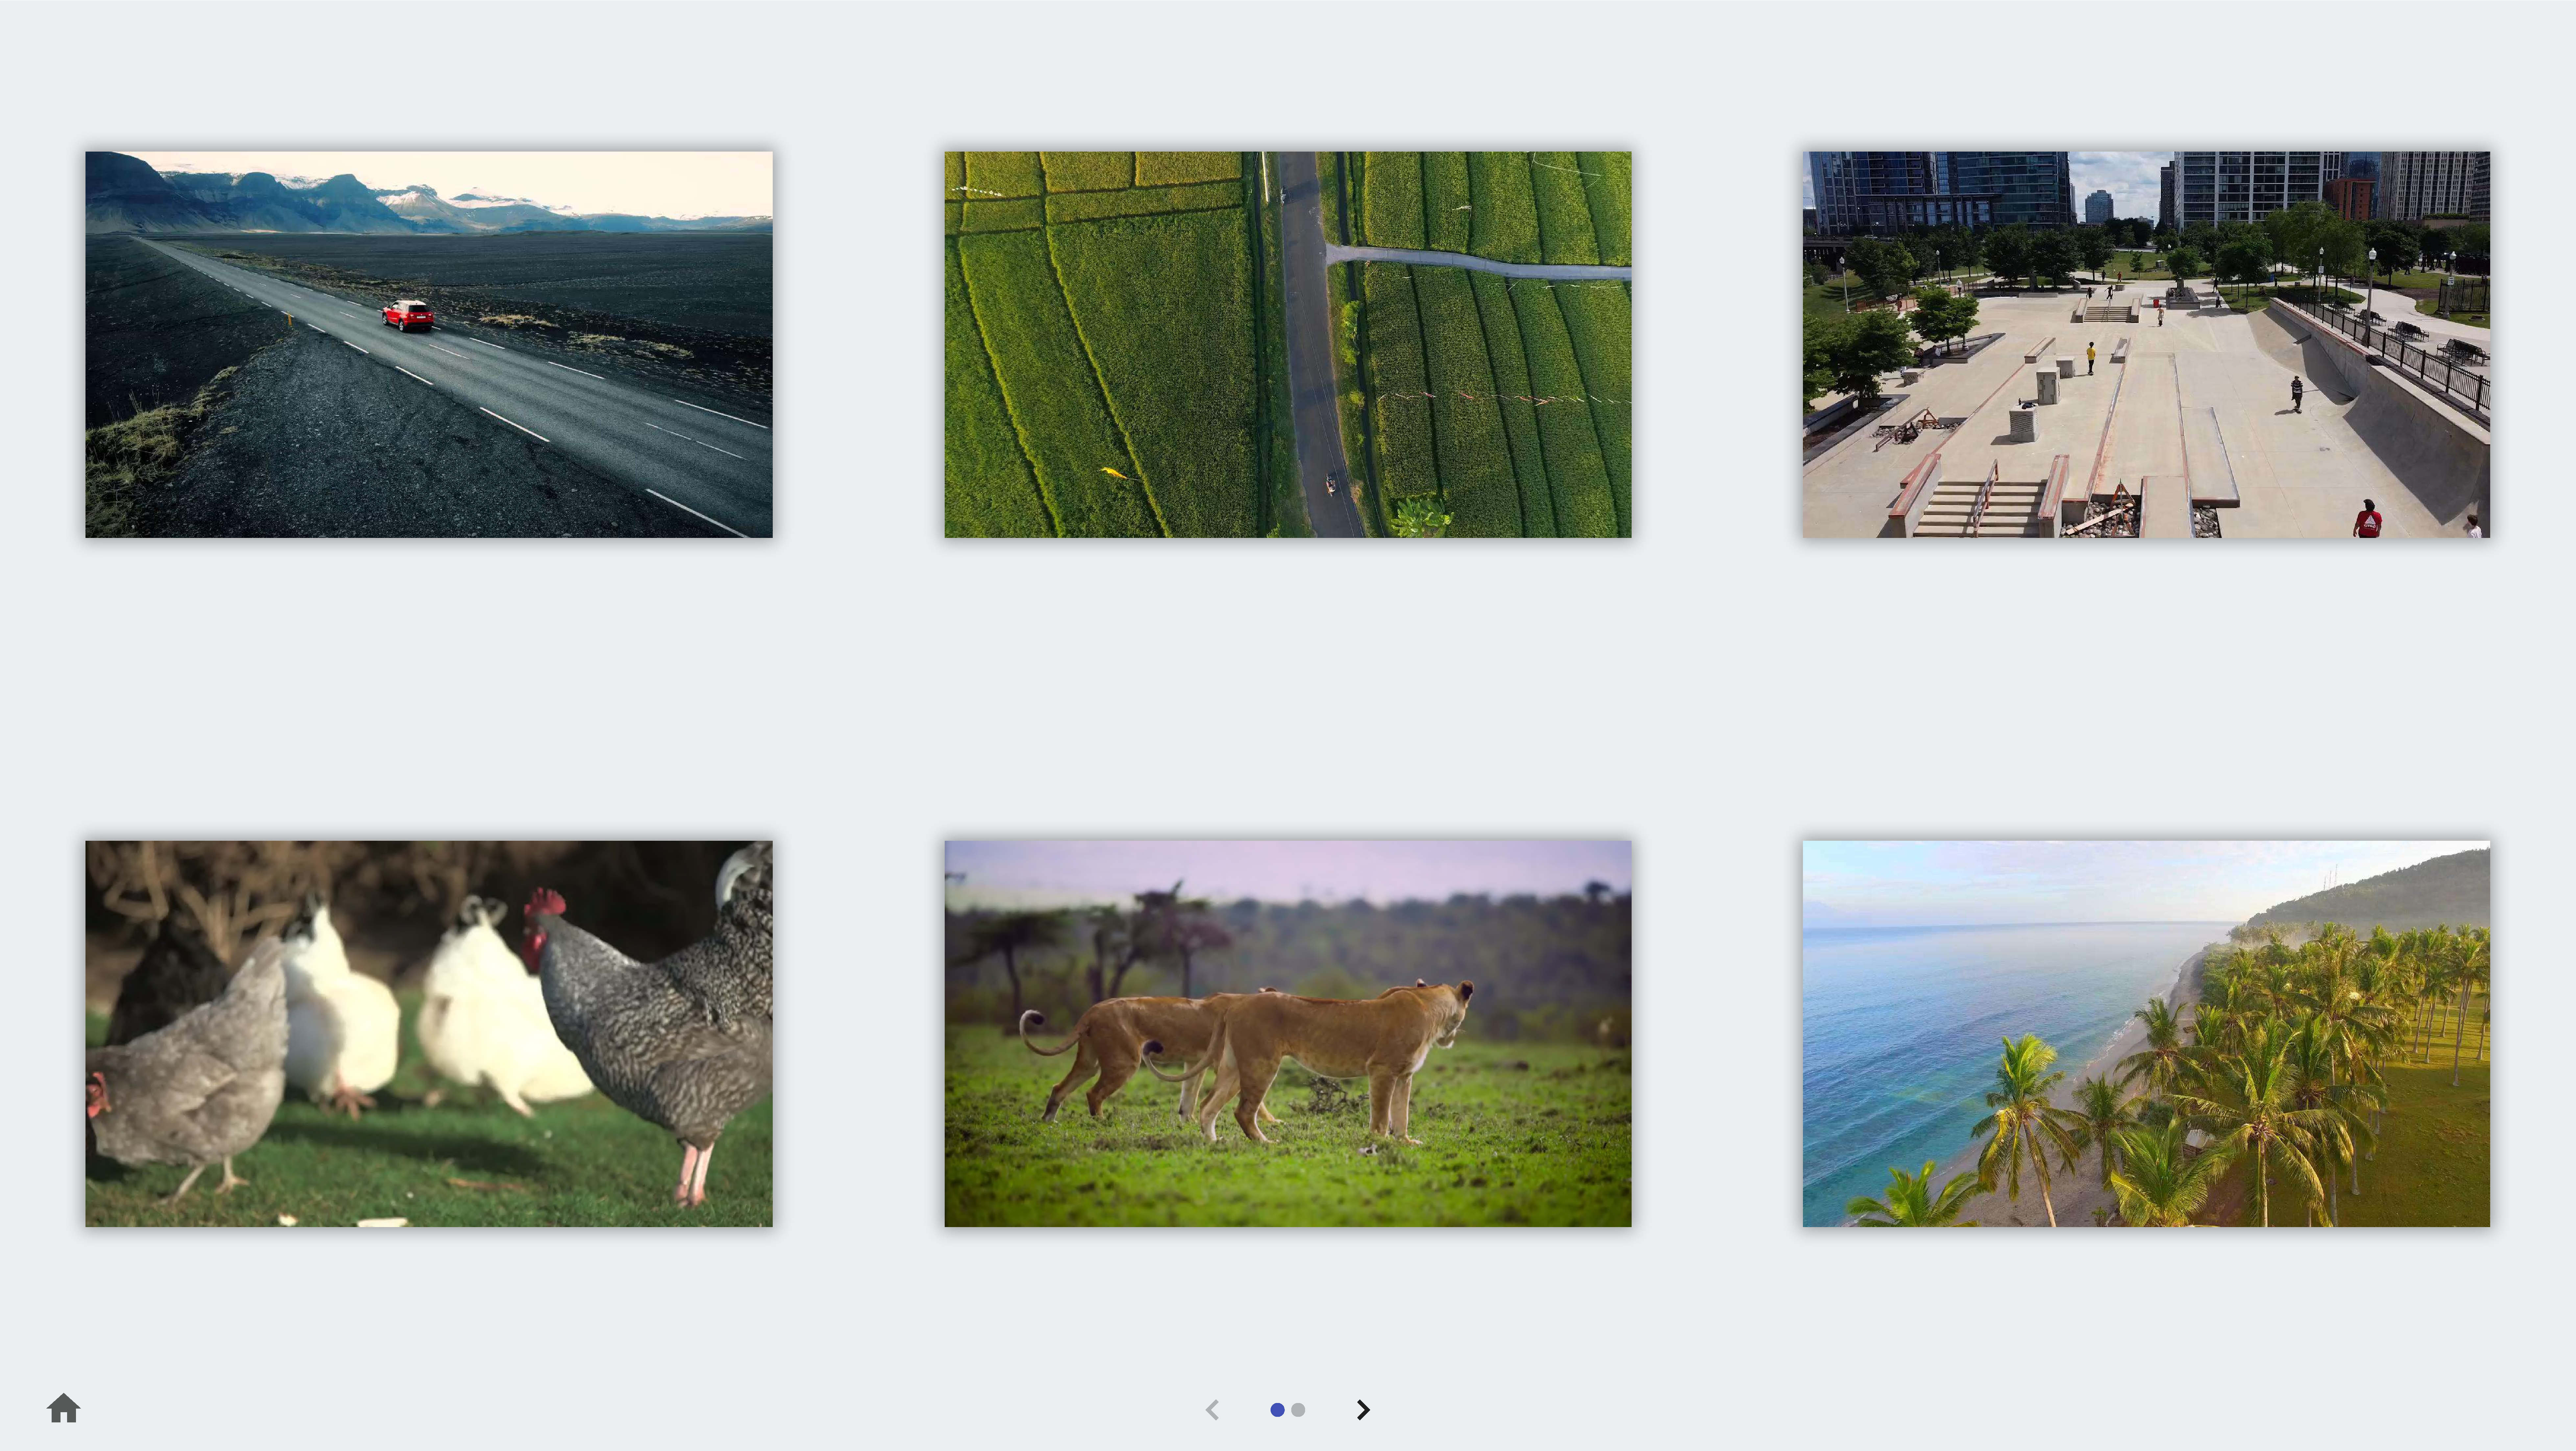
\includegraphics[width=.96\linewidth]{Figures/LUI/UI/videos-list.pdf} 
        \vspace{-5pt}
        \captionsetup{width=.9\linewidth}
        \caption{Videos app (list).}
        \label{fig:lui:screenshots:videos-list}
    \end{subfigure}
    \begin{subfigure}{.47\textwidth}
        \centering
        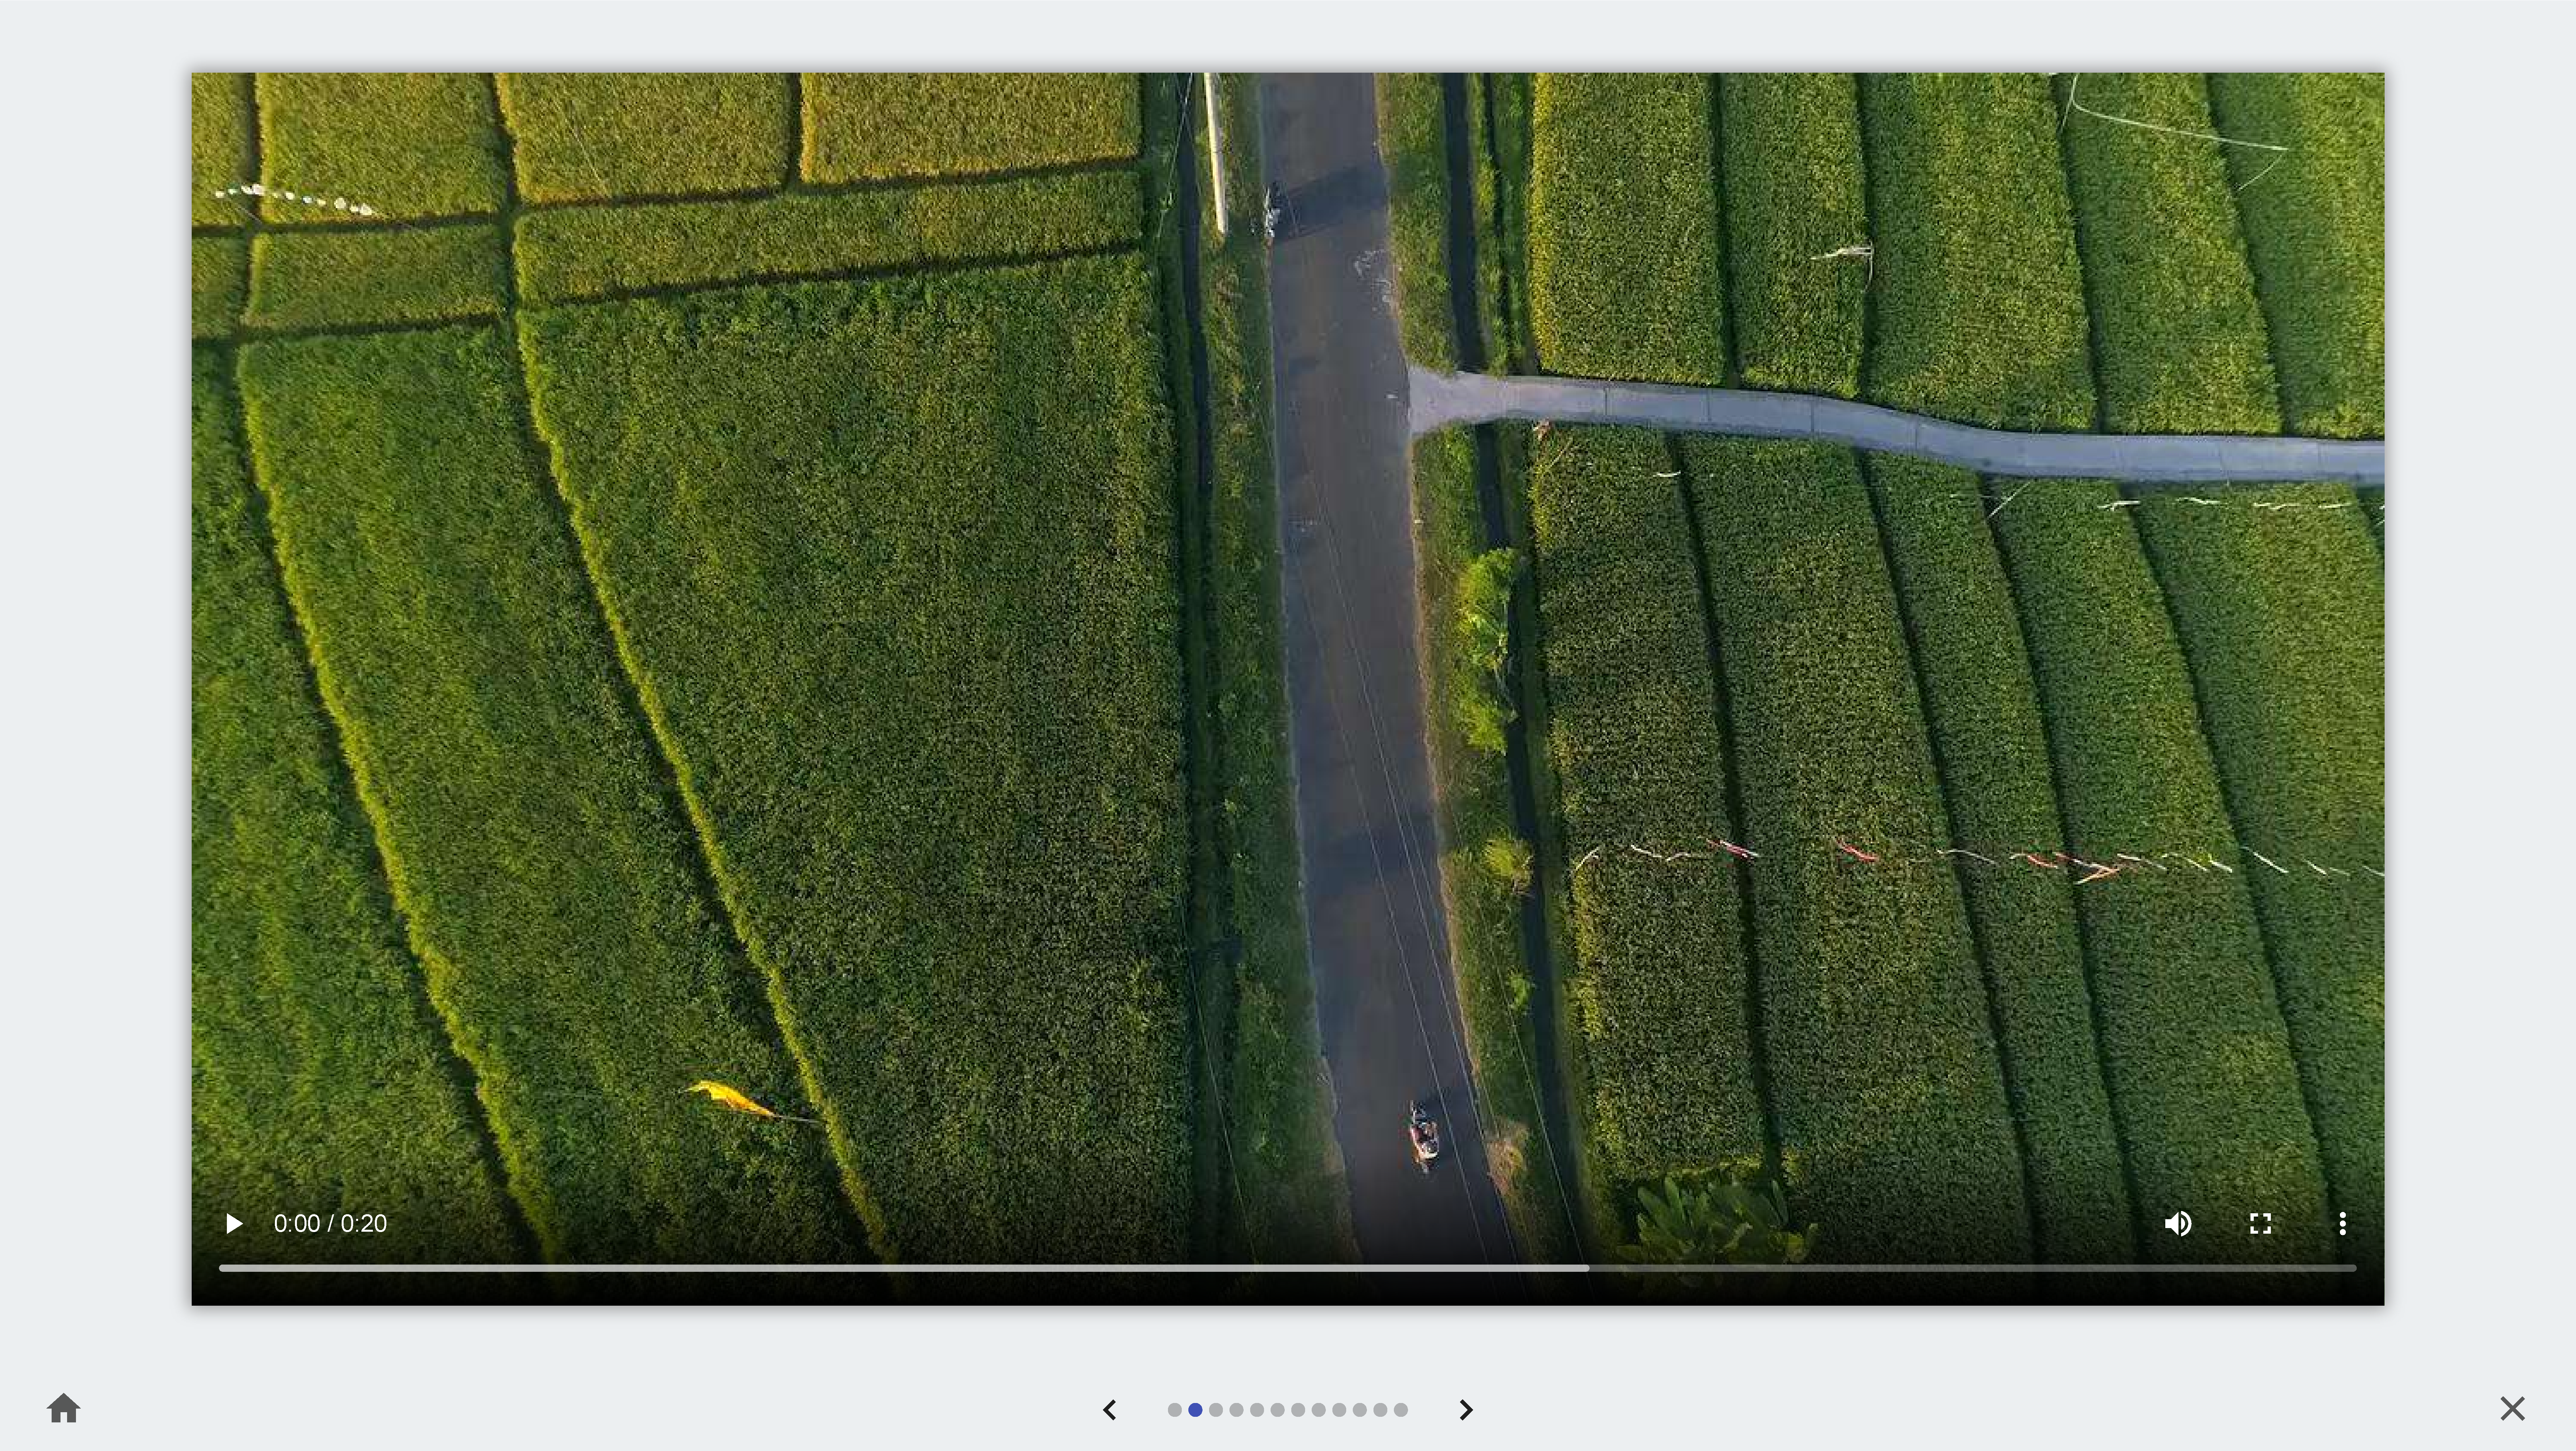
\includegraphics[width=.96\linewidth]{Figures/LUI/UI/videos-fullscreen.pdf}  
        \vspace{-5pt}
        \captionsetup{width=.9\linewidth}
        \caption{Videos app (item).}
        \label{fig:lui:screenshots:videos-fullscreen}
    \end{subfigure}

    \begin{subfigure}{.47\textwidth}
        \centering
        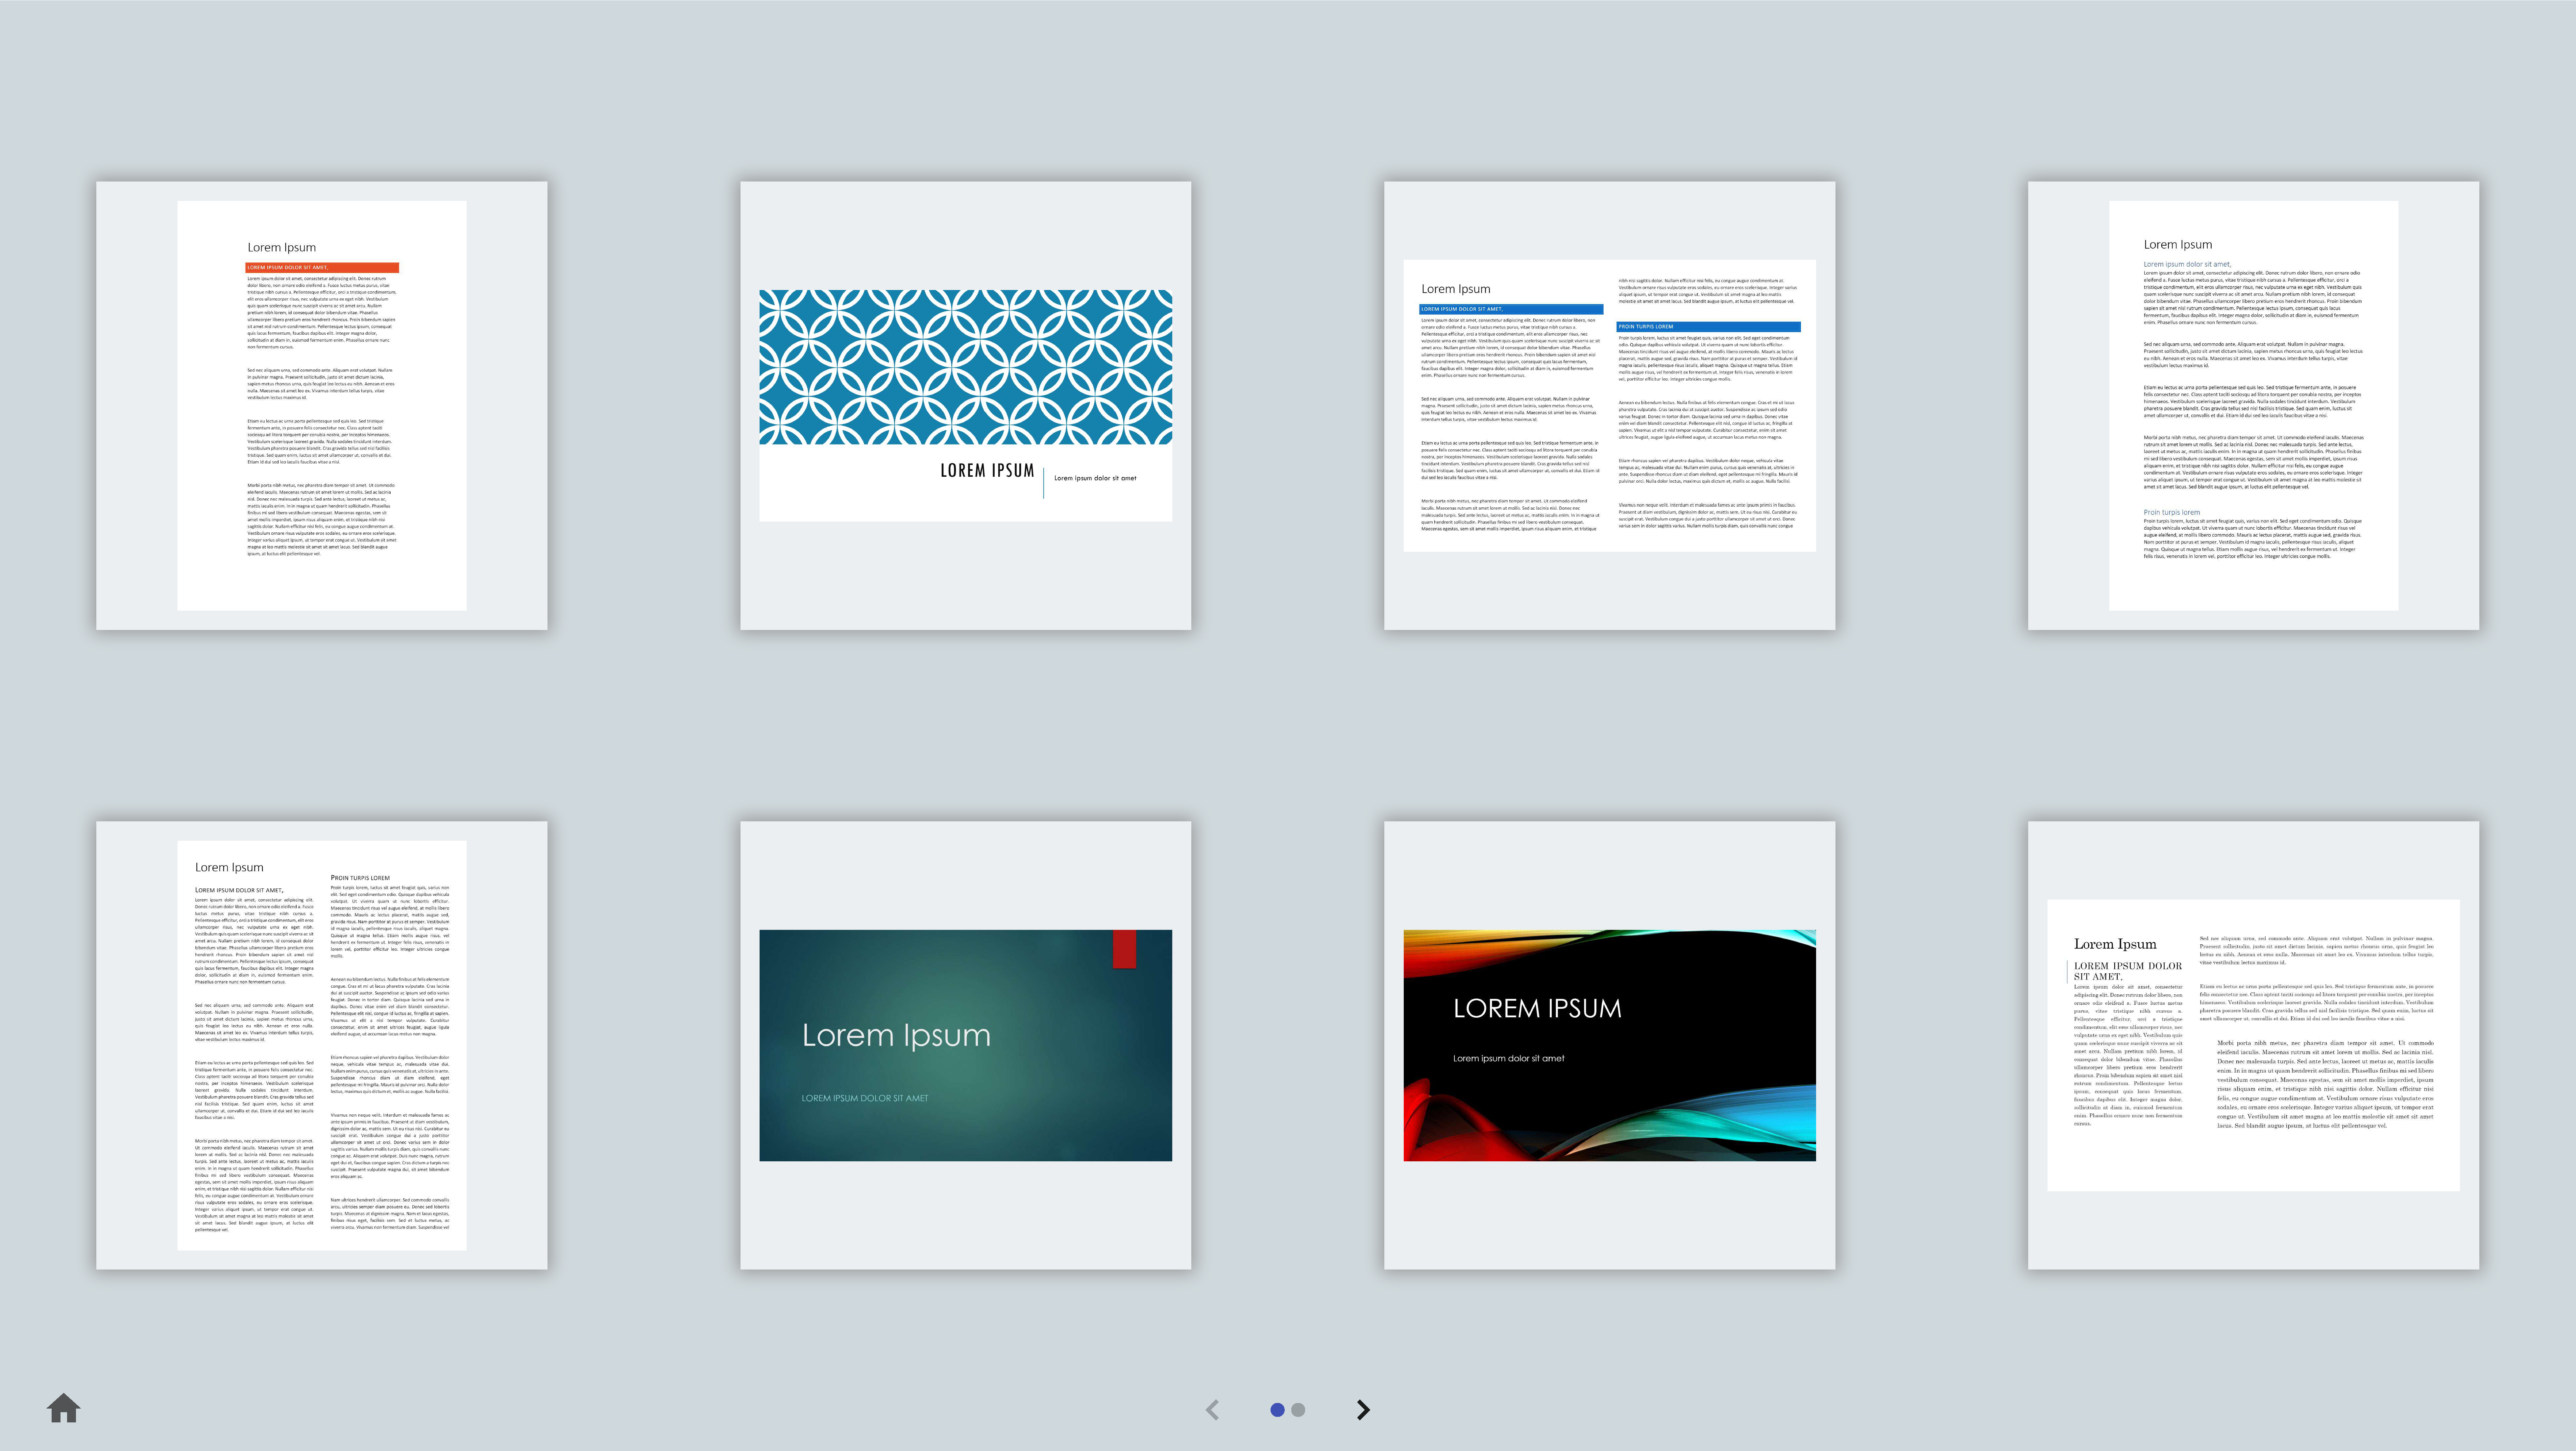
\includegraphics[width=.96\linewidth]{Figures/LUI/UI/documents-list.pdf} 
        \vspace{-5pt}
        \captionsetup{width=.9\linewidth}
        \caption{Documents app (list).}
        \label{fig:lui:screenshots:documents-list}
    \end{subfigure}
    \begin{subfigure}{.47\textwidth}
        \centering
        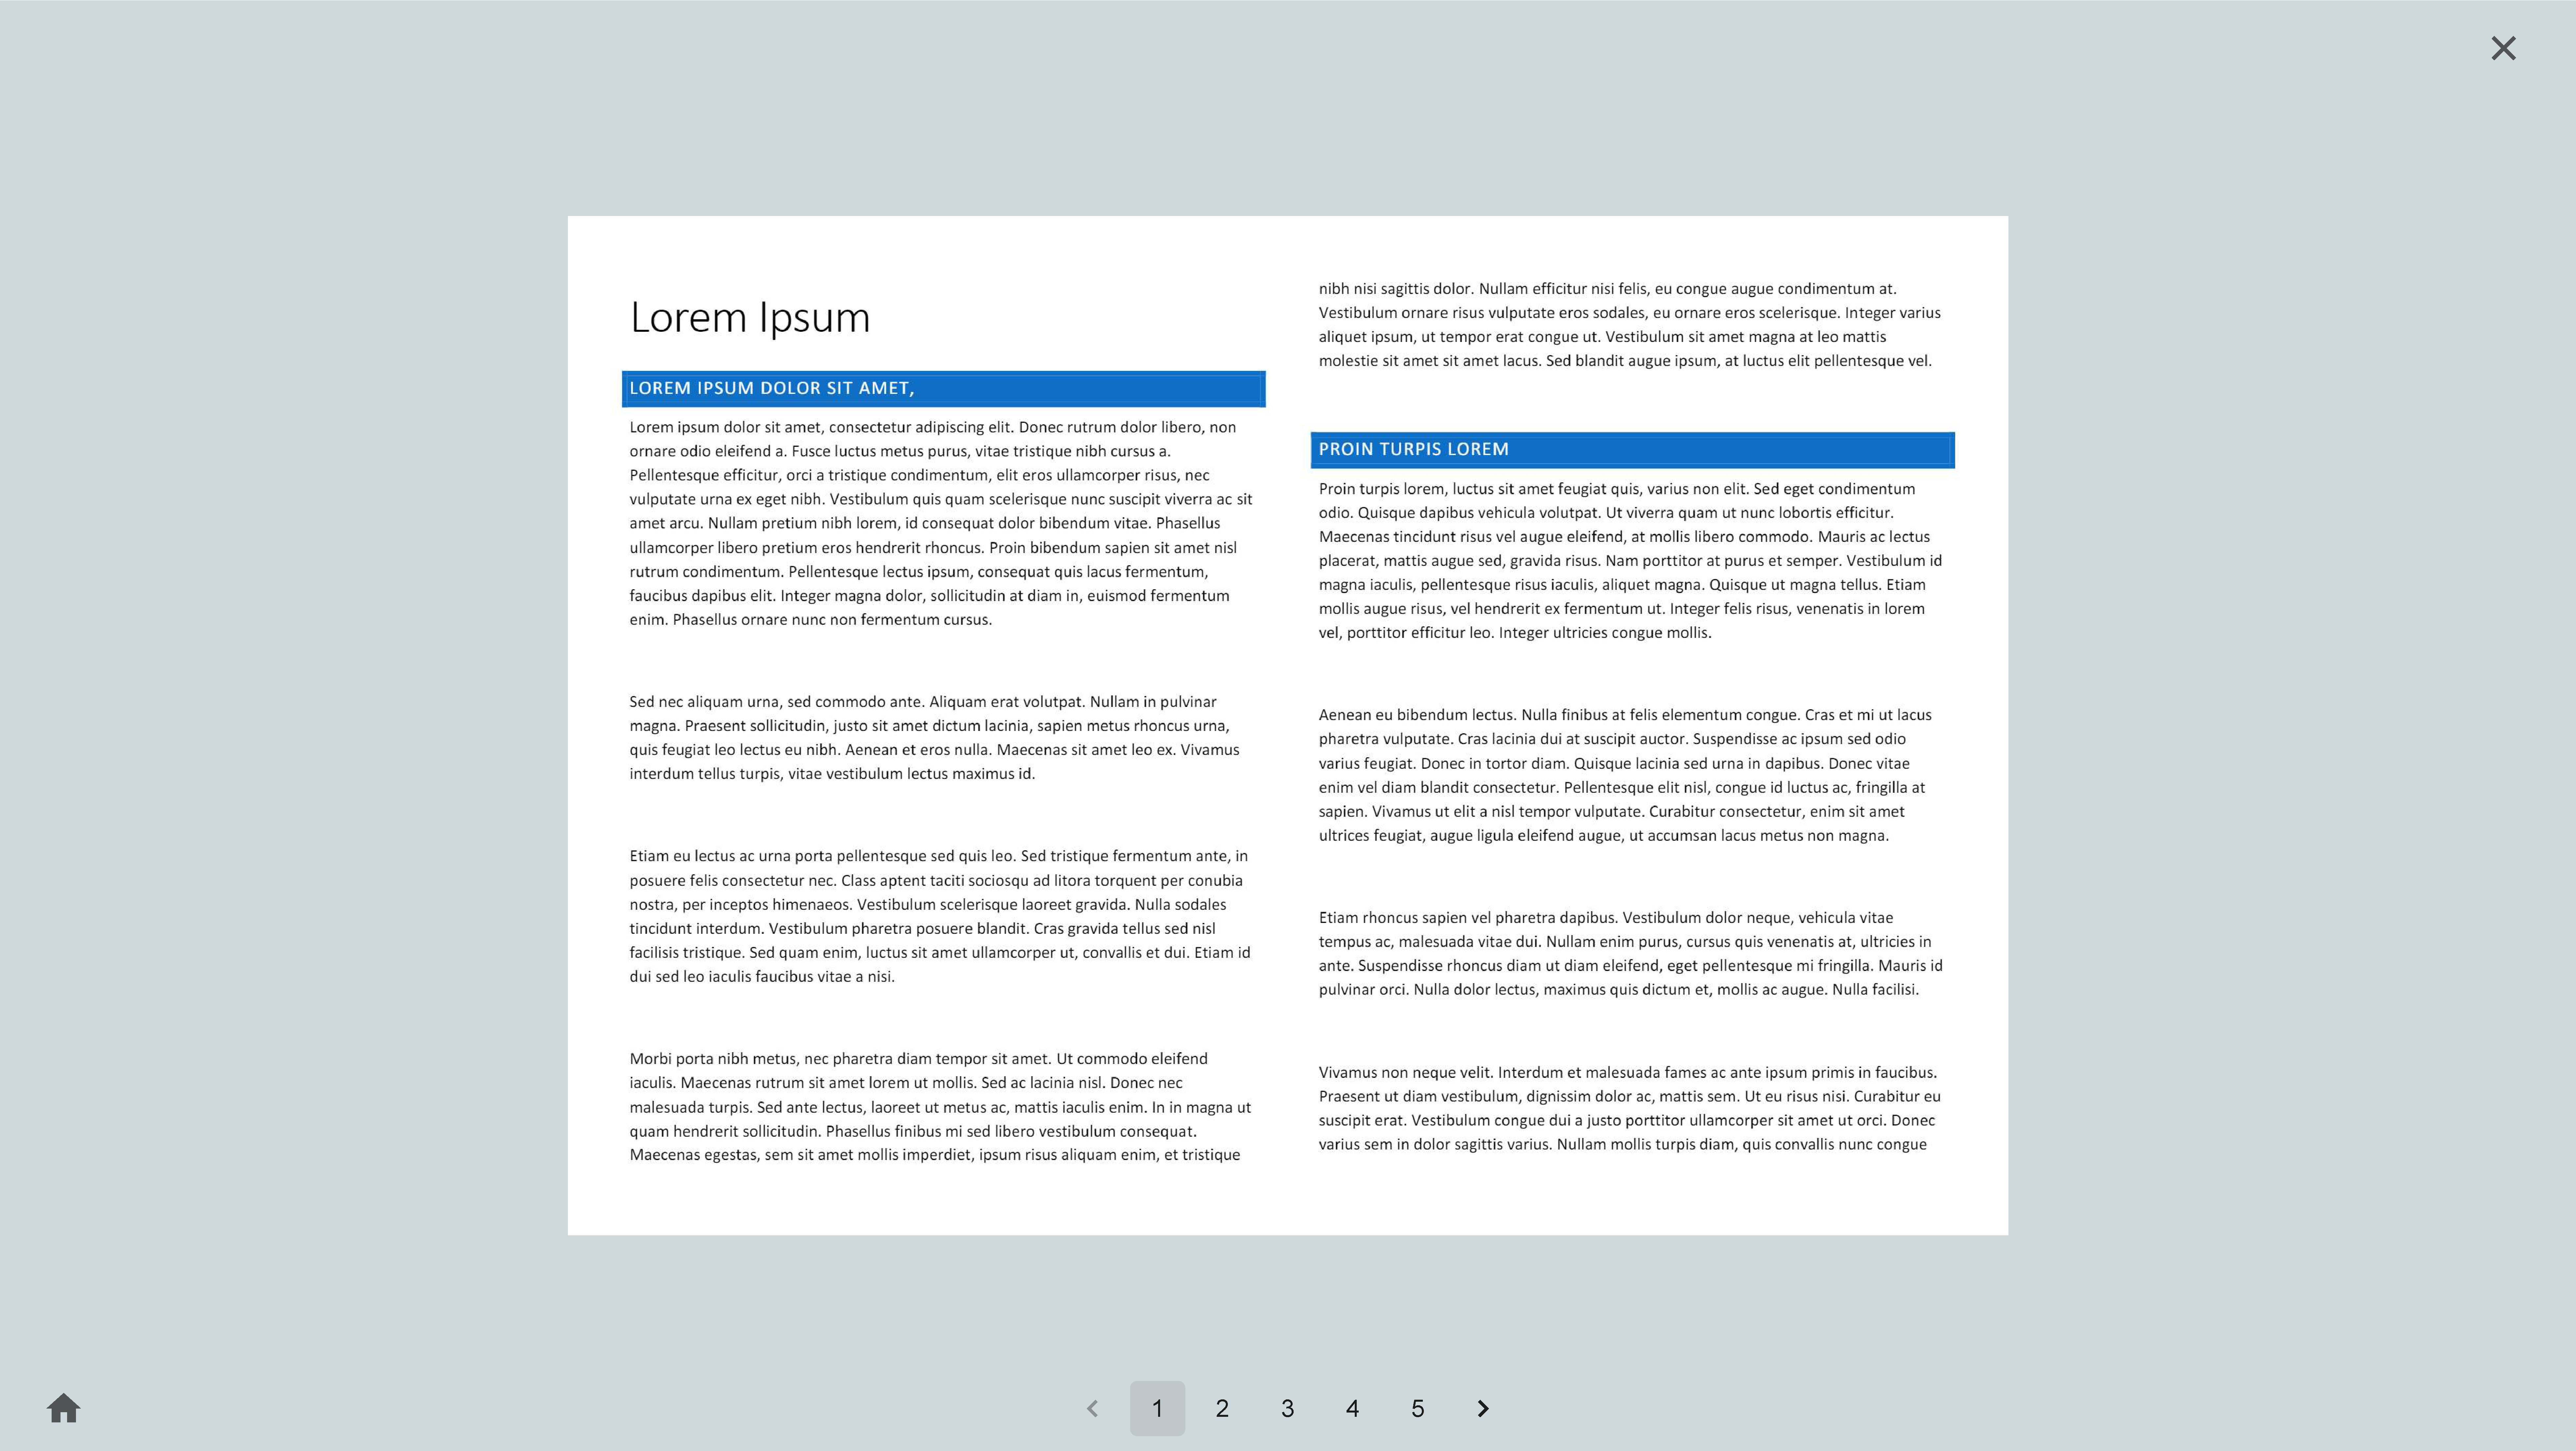
\includegraphics[width=.96\linewidth]{Figures/LUI/UI/documents-fullscreen.pdf}  
        \vspace{-5pt}
        \captionsetup{width=.9\linewidth}
        \caption{Documents app (item).}
        \label{fig:lui:screenshots:documents-fullscreen}
    \end{subfigure}

    \begin{subfigure}{.47\textwidth}
        \centering
        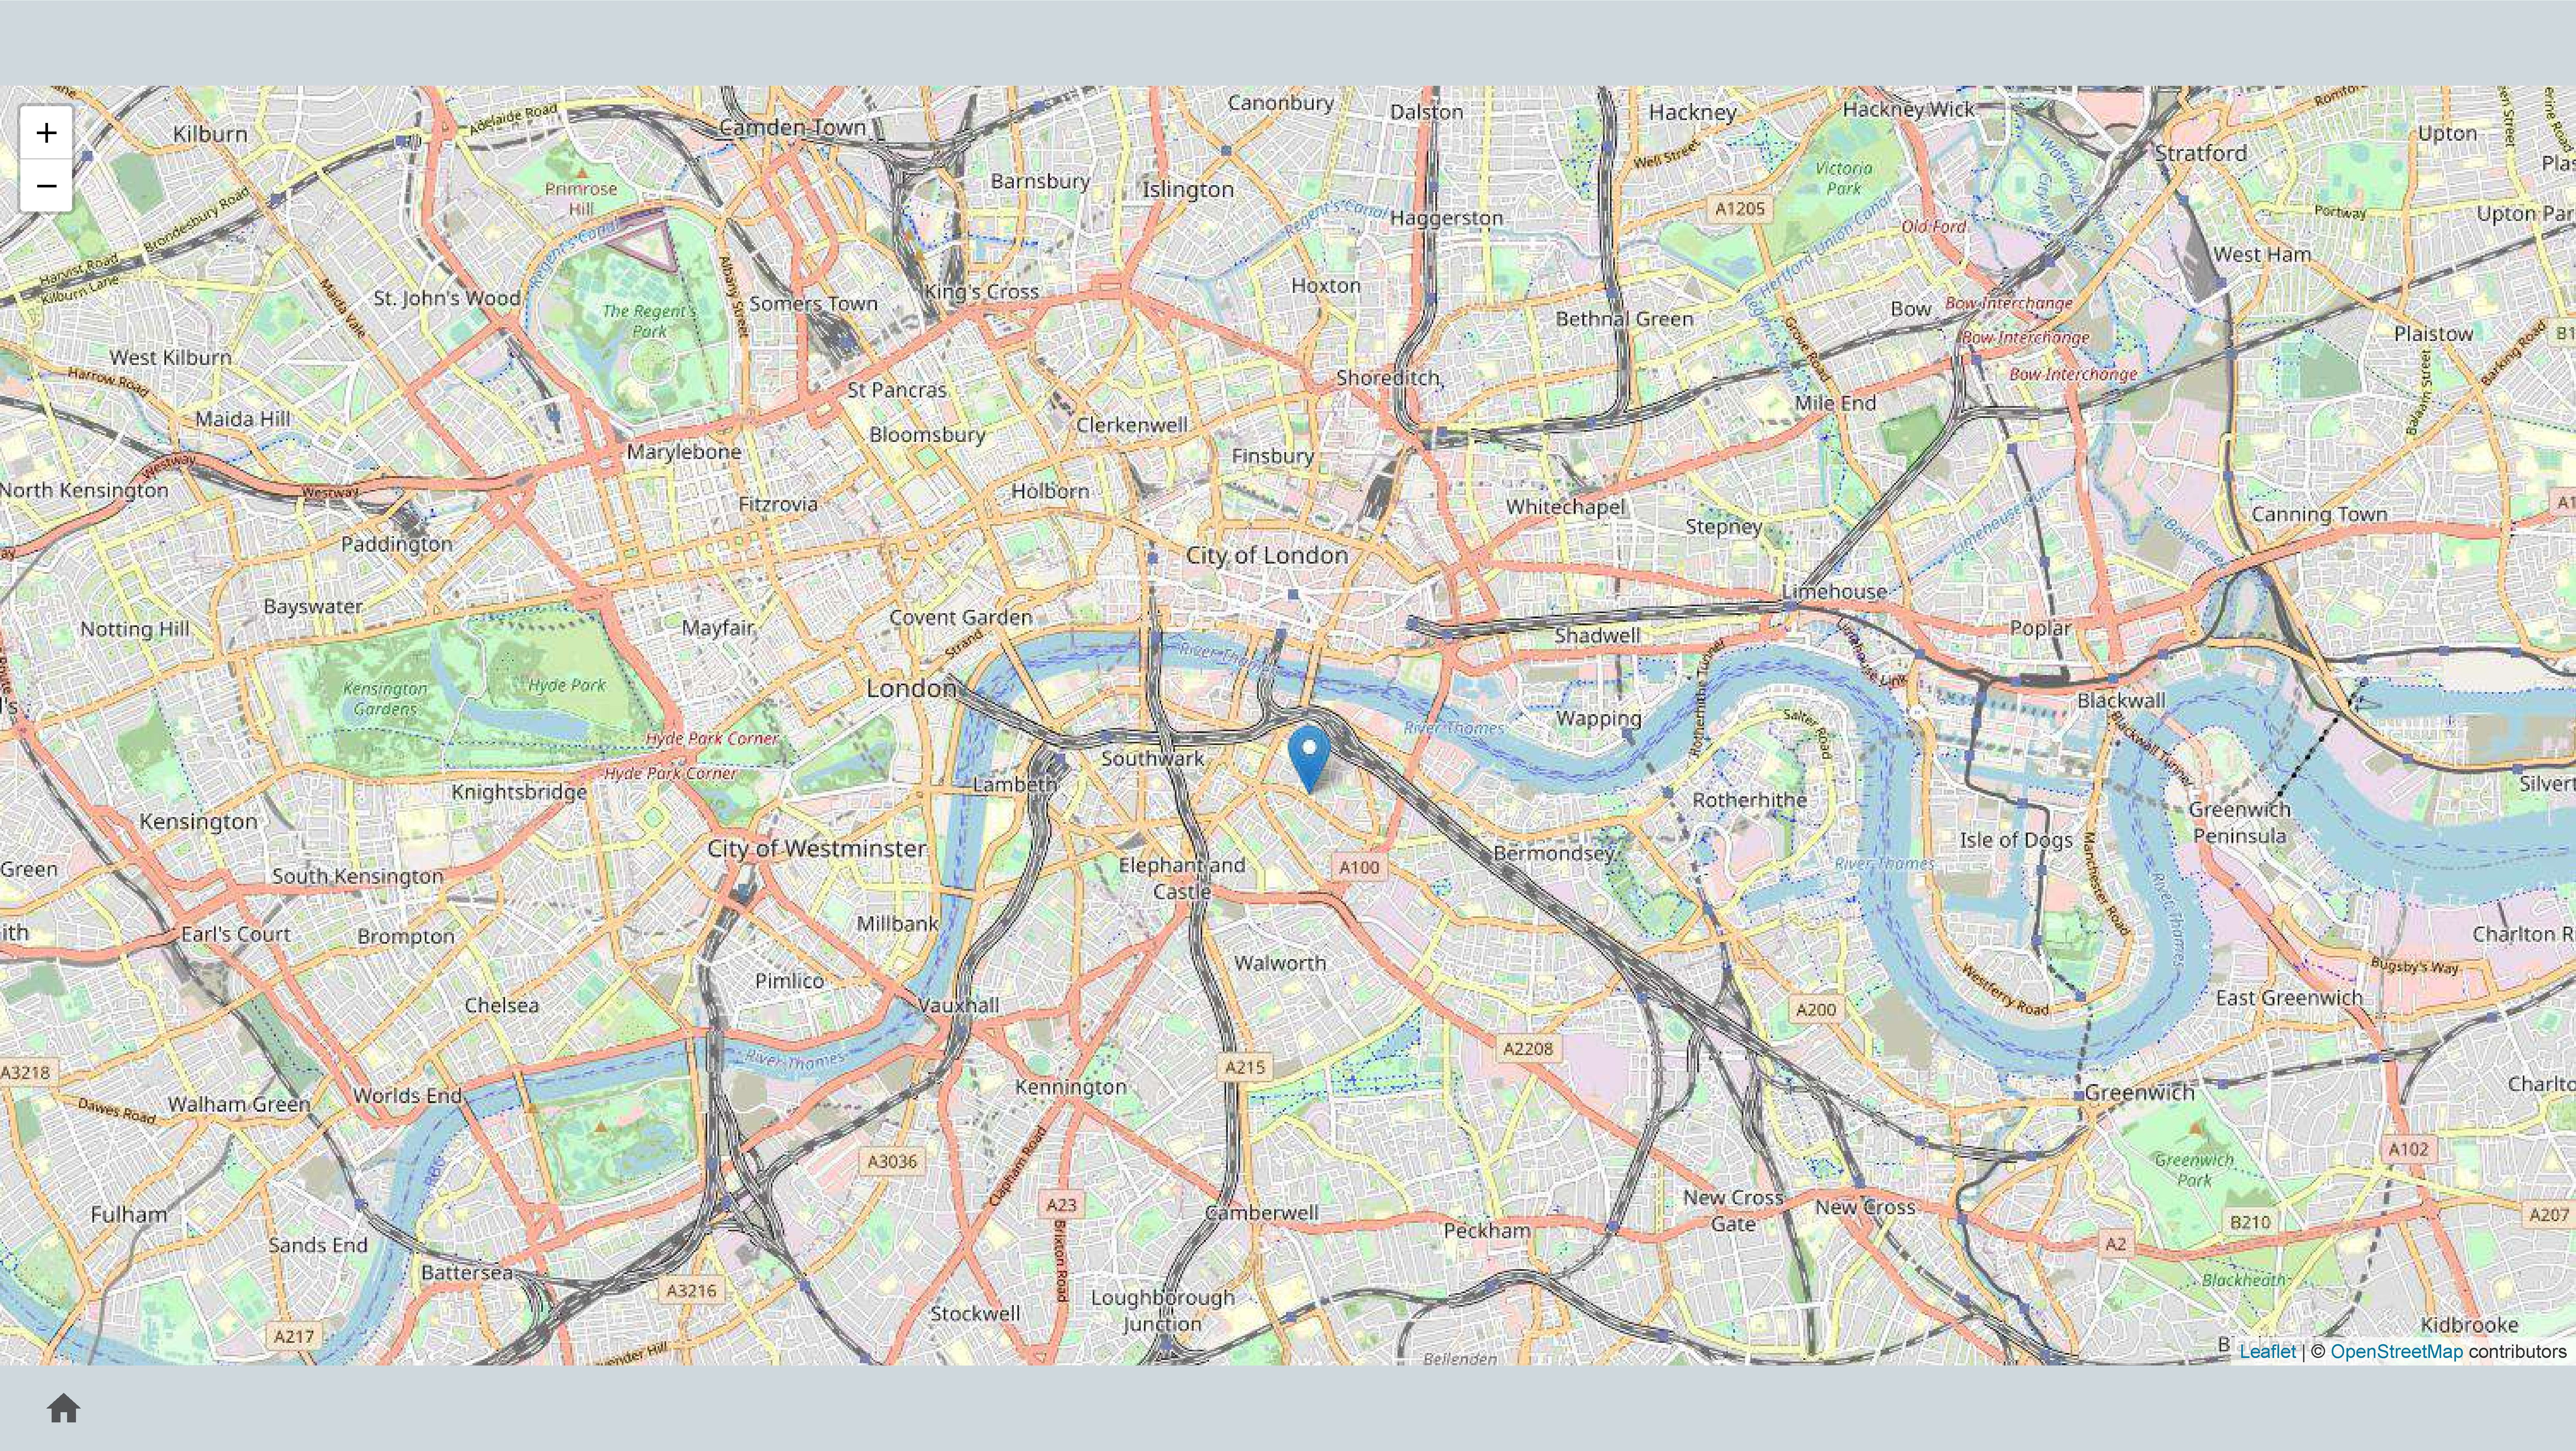
\includegraphics[width=.96\linewidth]{Figures/LUI/UI/maps.pdf} 
        \vspace{-5pt}
        \captionsetup{width=.9\linewidth}
        \caption{Maps app.}
        \label{fig:lui:screenshots:maps}
    \end{subfigure}
    \begin{subfigure}{.47\textwidth}
        \centering
        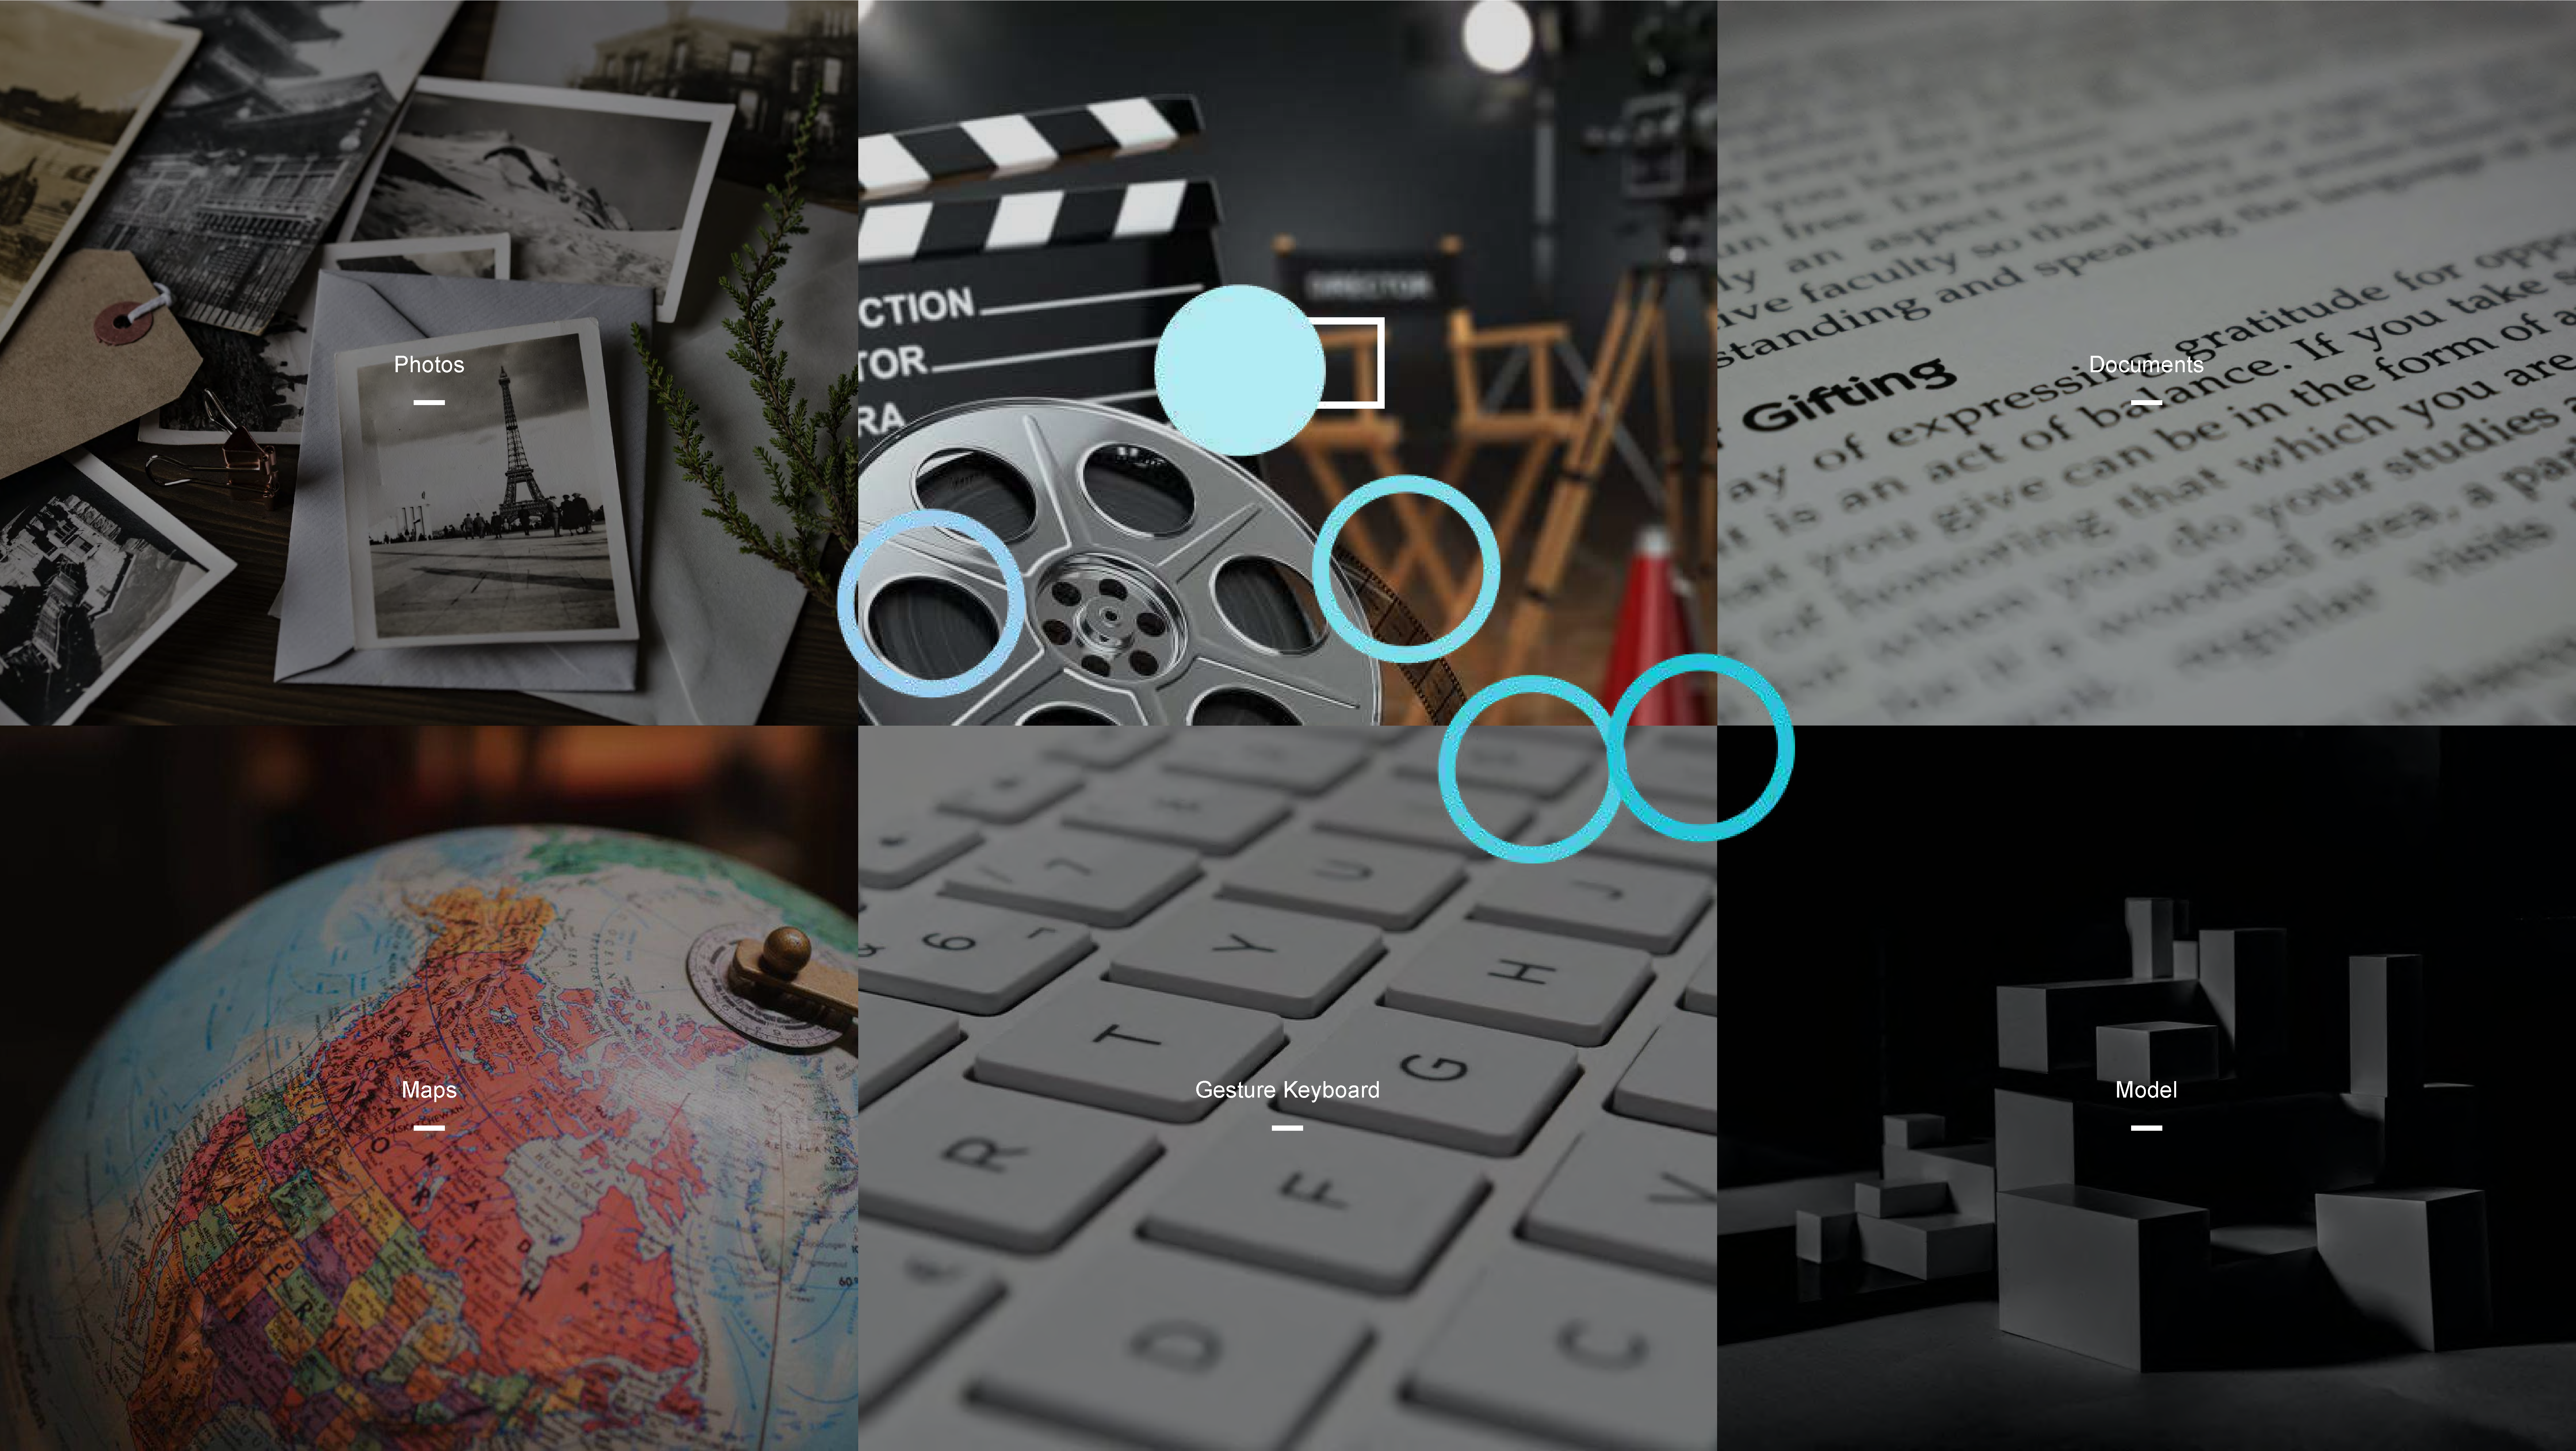
\includegraphics[width=.96\linewidth]{Figures/LUI/UI/fingers.pdf} 
        \vspace{-5pt}
        \captionsetup{width=.9\linewidth}
        \caption{User's hand.}
        \label{fig:lui:screenshots:hand}
    \end{subfigure}
    
    \vspace{-4pt}
    \caption{Screenshots of the third prototype of the \lui application.}
    % \vspace{-14pt}
    \label{fig:lui:screenshots}
\end{figure}

%--------------------------------------------------------------------------------%
\subsection{Requirements} \label{sec:lui:description:requirements}
To address the quality of the gesture interaction, \lui should fulfill three requirements:

\begin{enumerate}[noitemsep]
    \item \textit{Consistency.} Similar gestures should be assigned consistently to similar functions, independently of the media type, to foster knowledge transfer~\cite{Dingler:2018}, to maximize gesture memorability, and to reduce the learning curve~\cite{Delamare:2019}. Distinguishable gestures should be assigned to other specific functions~\cite{Kohlsdorf:2013}.
    \item \textit{Continuity.} End users should be able to perform gestures continuously, without needing to notify the system when they are performing a gesture, \ie the system should continuously recognize gestures and distinguish intended gestures from parasitic motion with little to no user intervention. End users should be able to manipulate media objects directly with a reasonable system response time (\eg 1 sec for direct manipulation according to~\cite{Nielsen:1994}) and continuous feedback to the user~\cite{Aigner:2012} (\eg gradually zooming in a picture by increasing the distance between the index and the thumb). Whether a gesture is discrete for a 0D/1D function or continuous for a 2D/3D function, this should not induce any difference for the end user.
    \item \textit{Customizability.} The system should support users in including their own gestures without requiring any modification to the \lui core~\cite{Coyette:2007}. User-defined gesture sets~\cite{Grijincu:2014} usually result in higher satisfaction and memorability than system- or designer-defined gestures~\cite{Nacenta:2013}. Some gesture recognizers perform better when the gestures used for training are recorded by the target user of the system~\cite{Vatavu:2013}.
\end{enumerate}

%--------------------------------------------------------------------------------%
\subsection{Iterative Design} \label{sec:lui:description:iterative-design}
The \lui application went through two iterations before the final one described in this chapter. This section summarizes the three iterations of \lui and its gesture set (\fig~\ref{fig:lui:gesture-set-evolution}).

\begin{figure}[!b]
    \centering
    % \vspace{-6pt}
    \includegraphics[width=\linewidth]{Figures/LUI/Overview/gesture-set-evolution.pdf}
    \vspace{-8pt}
    \caption{Evolution of the gesture set during the iterative design.}
    \label{fig:lui:gesture-set-evolution}
    % \vspace{-16pt}
\end{figure}

\subsubsection{First Iteration (v1)}
In this first prototype~\cite{Parthiban:2019}, the basics of \lui were laid out. Users could navigate through lists of photos and videos, switch to full-screen mode, and play, pause, or change the volume of a video. Gesture recognition was developed opportunistically based on the LMC API~\cite{Spiegelmock:2013}, which made adding new functions or gestures to \lui a complex endeavor and resulted in a rather small set of gestures. End users were thus forced to use the predefined gestures, with no possibility of assigning their own gestures to specific functions.

\subsubsection{Second Iteration (v2)}
A usability testing was conducted with 20 participants to evaluate their subjective satisfaction regarding the first prototype~\cite{Parthiban:2019,Dumas:2019}. It highlighted multiple issues, including a high learning curve, unpredictable gesture recognition, and fatigue, in particular for the \textit{splay} gesture, which participants found especially difficult to perform and reproduce accurately. 
Some participants expressed their intention to define their own preferred gestures, instead of using the predefined ones.
This second prototype replaced the \textit{splay} gesture with the \textit{flick up} gesture, which is easier to perform. Other issues highlighted by the testing were left unaddressed in this version, as they required more substantial modifications to the \lui core.

\subsubsection{Third Iteration (v3)}
The current version of \lui was developed based on the assets of the first two prototypes but features significant changes to its gesture set and gesture recognition pipeline (Section~\ref{sec:lui:development-method}). 
It now relies on the \ql pipeline for gesture recognition, which enables end users to add their own preferred gestures to predefined ones without having to modify the \lui core. The use of \ql also vastly simplified the process of extending \lui with new applications and gestures, which enabled us to add new functions to the Photos and Videos applications (\eg rotating a photo and browsing through a video), and implement new Documents and Maps applications.

%================================================================================%
\section{User-centered Development Method} \label{sec:lui:development-method}
This section details the three-stage development process that we followed for the third iteration of \lui. 
%
We first designed an intuitive set of gestures, consistent across the entire \lui application, based on the results of a GES. 
%
Then, we ran a comparative testing of static and dynamic gesture recognizers using the \ql testing tool (Chapter~\ref{chap:quantumleap-testing}) to identify a suitable dataflow configuration for this gesture set.
%
Finally, we instantiated a gesture recognition dataflow based on the results of our testing using the \ql framework (Chapter~\ref{chap:quantumleap}).

%--------------------------------------------------------------------------------%
\subsection{Gesture Set Design} \label{sec:lui:development-method:gesture-set}
\subsubsection{Gesture Identification}
As the number of functions increased, it was decided to conduct a GES~\cite{Wobbrock:2009} to explore a consensus set of consistent gestures that would optimize agreement among end users. Based on the classical method~\cite{Wobbrock:2009} and some extensions~\cite{Gheran:2018}, we initially conducted two GESs (see Appendix~\ref{app:lui-ges:initial}): one for photo browsing and another for video browsing. Prior work~\cite{Anthony:2013,Groenewald:2016} pointed out that gesture sets for different devices could be inconsistent. Our two studies confirm this observation as they led to inconsistent gestures tailored to one media type at a time. 
Rather than conducting a separate GES for each media type, we conducted a single GES (see Appendix~\ref{app:lui-ges:new}) integrating the various media with both generic and specific functions.

The result of our GES consists of a characterization of users' gesture input behaviors with valuable information for designers, practitioners, and end users regarding the consensus among participants (which is computed as an \textit{agreement} and \textit{co-agreement rate}~\cite{Vatavu:2015}), most frequent (thus, generalizable across users) gestures for a specified task, and insights into users' conceptual models for performing tasks. \cite{Dingler:2018} computed the agreement score~\cite{Wobbrock:2009} for their multi-device GES. Instead, we computed the agreement rate $AR(r)$~\cite{Vatavu:2015}, which is smaller and more restrictive than the agreement score $A(r)$, as follows:
\vspace{-5pt}
\begin{equation}
A(r) = \sum_{P_i \subseteq P} {\Bigg( \frac{\lvert P_i \vert}{\lvert P \vert} \Bigg)}^2
\geq
AR(r)= \frac{
\sum_{P_i\subseteq P} {\frac{1}{2} \lvert P_i \vert  \:(\lvert P_i \vert{-}1)}}
{\frac{1}{2} \lvert P \vert   \:(\lvert P \vert{-}1)}
\label{eq:agreement1}
\end{equation}
%\vspace{-3pt}
where $r$ denotes the referent to elicit a gesture, $\lvert P \rvert$ denotes the number of elicited gestures, and $\vert P_{i} \rvert$ denotes the number of gestures elicited for the $i^{th}$ subgroup of $P$. 


\tab~\ref{tbl:lui-ges:gesture-proposals} summarizes the two most agreed gestures for each referent of the GES. 
% One-handed
From these results, we observe that the majority ($\frac{16}{18} {=} 88.9\%$) of the most agreed gestures were one-handed. One-handed gestures let users interact with the system while holding an object in the other hand (\eg a glass of water or a paper document). In addition, the low occurrence of two-handed gestures in our study may be explained by a lower ease of execution compared to one-handed gestures~\cite{Morris:2010}.
% User-defined gestures + indirect method
Some referents, such as enable/disable subtitles, have a very low agreement rate. For these referents, user-elicited gestures may not be the most appropriate, as the low consensus may result in lower guessability and memorability~\cite{Wobbrock:2005}. Instead, it may be preferable to favor other solutions, such as prompting users to assign their own gesture to these actions at the start of the application (\ie user-defined gestures~\cite{Nacenta:2013}), and/or providing an indirect way of triggering these actions (\eg by navigating through a menu with highly agreed gestures).
% Aliasing
For referents with a low to medium agreement rate, such as play and pause, aliasing (\ie assign multiple gestures, such as the most and second most agreed gestures, to one referent) may greatly increase guessability~\cite{Wobbrock:2005, Wobbrock:2009}. This would enable users to use the gesture they are most familiar with, and thus flatten the learning curve and increase the memorability of the gesture set. However, attentive care should be given to avoid overloading gestures.

\begin{figure}[ht]
    \begin{subfigure}{.24\textwidth}
        \centering
        \includegraphics[width=.97\linewidth]{Figures/LUI/Gestures/flick_right.pdf}  
        \vspace{-6pt}
        \captionsetup{width=.9\linewidth}
        \caption{Previous.}
        \label{fig:lui:gestures:previous}
    \end{subfigure}
    \begin{subfigure}{.24\textwidth}
        \centering
        \includegraphics[width=.97\linewidth]{Figures/LUI/Gestures/flick_left.pdf}  
        \vspace{-6pt}
        \captionsetup{width=.9\linewidth}
        \caption{Next.}
        \label{fig:lui:gestures:next}
    \end{subfigure}
    \begin{subfigure}{.24\textwidth}
        \centering
        \includegraphics[width=.97\linewidth]{Figures/LUI/Gestures/tap-open.pdf} 
        \vspace{-6pt}
        \captionsetup{width=.99\linewidth}
        \caption{Enable fullscreen.}
        \label{fig:lui:gestures:fullscreen-on}
    \end{subfigure}
    \begin{subfigure}{.24\textwidth}
        \centering
        \includegraphics[width=.97\linewidth]{Figures/LUI/Gestures/flick_up.pdf} 
        \vspace{-6pt}
        \captionsetup{width=.99\linewidth}
        \caption{Disable fullscreen.}
        \label{fig:lui:gestures:fullscreen-off}
    \end{subfigure}
    
    \begin{subfigure}{.24\textwidth}
        \centering
        \includegraphics[width=.97\linewidth]{Figures/LUI/Gestures/pinch_out.pdf}
        \vspace{-6pt}
        \captionsetup{width=.9\linewidth}
        \caption{Zoom in.}
        \label{fig:lui:gestures:zoom-in}
    \end{subfigure}
    \begin{subfigure}{.24\textwidth}
        \centering
        \includegraphics[width=.97\linewidth]{Figures/LUI/Gestures/pinch_in.pdf} 
        \vspace{-6pt}
        \captionsetup{width=.9\linewidth}
        \caption{Zoom out.}
        \label{fig:lui:gestures:zoom-out}
    \end{subfigure}
    \begin{subfigure}{.24\textwidth}
        \centering
        \includegraphics[width=.97\linewidth]{Figures/LUI/Gestures/swipe_up-volume.pdf}  
        \vspace{-6pt}
        \captionsetup{width=.9\linewidth}
        \caption{Volume up.}
        \label{fig:lui:gestures:volume-up}
    \end{subfigure}
    \begin{subfigure}{.24\textwidth}
        \centering
        \includegraphics[width=.97\linewidth]{Figures/LUI/Gestures/swipe_down-volume.pdf}  
        \vspace{-6pt}
        \captionsetup{width=.9\linewidth}
        \caption{Volume down.}
        \label{fig:lui:gestures:volume-down}
    \end{subfigure}

    \begin{subfigure}{.24\textwidth}
        \centering
        \includegraphics[width=.97\linewidth]{Figures/LUI/Gestures/rotate_clockwise.pdf}  
        \vspace{-6pt}
        \captionsetup{width=.9\linewidth}
        \caption{Rotate clockwise.}
        \label{fig:lui:gestures:rotate-anticlock}
    \end{subfigure}
    \begin{subfigure}{.24\textwidth}
        \centering
        \includegraphics[width=.97\linewidth]{Figures/LUI/Gestures/rotate_counterclockwise.pdf}  
        \vspace{-6pt}
        \captionsetup{width=.9\linewidth}
        \caption{Rotate anti-clock.}
        \label{fig:lui:gestures:rotate-clock}
    \end{subfigure}
    \begin{subfigure}{.24\textwidth}
        \centering
        \includegraphics[width=.97\linewidth]{Figures/LUI/Gestures/tap-play.pdf} 
        \vspace{-6pt}
        \captionsetup{width=.9\linewidth}
        \caption{Play/pause.}
        \label{fig:lui:gestures:play-pause}
    \end{subfigure}
    \begin{subfigure}{.24\textwidth}
        \centering
        \includegraphics[width=.97\linewidth]{Figures/LUI/Gestures/thumb_up.pdf} 
        \vspace{-6pt}
        \captionsetup{width=.9\linewidth}
        \caption{Like.}
        \label{fig:lui:gestures:like}
    \end{subfigure}

    \begin{subfigure}{.24\textwidth}
        \centering
        \includegraphics[width=.97\linewidth]{Figures/LUI/Gestures/thumb_down.pdf}  
        \vspace{-6pt}
        \captionsetup{width=.9\linewidth}
        \caption{Dislike.}
        \label{fig:lui:gestures:dislike}
    \end{subfigure}
    \begin{subfigure}{.24\textwidth}
        \centering
        \includegraphics[width=.97\linewidth]{Figures/LUI/Gestures/swipe_left-seek.pdf}  
        \vspace{-6pt}
        \captionsetup{width=.9\linewidth}
        \caption{Fast forward.}
        \label{fig:lui:gestures:fast-forward}
    \end{subfigure}
    \begin{subfigure}{.24\textwidth}
        \centering
        \includegraphics[width=.97\linewidth]{Figures/LUI/Gestures/swipe_right-seek.pdf}  
        \vspace{-6pt}
        \captionsetup{width=.9\linewidth}
        \caption{Rewind.}
        \label{fig:lui:gestures:rewind}
    \end{subfigure}
    \begin{subfigure}{.24\textwidth}
        \centering
        \includegraphics[width=.97\linewidth]{Figures/LUI/Gestures/pan.pdf}  
        \vspace{-6pt}
        \captionsetup{width=.9\linewidth}
        \caption{Pan.}
        \label{fig:lui:gestures:pan}
    \end{subfigure}
    % \vspace{-4pt}
    \caption{Illustrations of gestures mapped to each function in the \lui application.}
    \label{fig:lui:gestures}
%    \vspace{-6pt}
\end{figure}

\subsubsection{Gestures Selection} 
The \lui gesture set (\fig~\ref{fig:lui:gestures} and \tab~\ref{tab:lui:elicitation-to-recognition}) resulting from the contextual GES consists of gestures selected following four guidelines inspired by the literature~\cite{Morris:2010,Wobbrock:2005,Wobbrock:2009,Dingler:2018}:
\begin{enumerate}[noitemsep]
    \item Favor the most agreed gestures, as this usually results in a flatter learning curve and higher memorability~\cite{Wobbrock:2005,Wobbrock:2009,Dingler:2018}. For instance, we selected ``flick left'' instead of ``flick right'' for the ``next'' function, as the former was proposed by more participants.
    \item Prefer gestures that are less physically and mentally demanding to limit frustration and fatigue~\cite{Morris:2010}. For example, we favored one-handed over two-handed gestures.
    \item Map similar gestures to similar functions, independently of the media to increase memorability and flatten the learning curve~\cite{Dingler:2018}. For instance, we selected the same gesture for zooming in a photo/in a map and used symmetrical gestures for going to the previous/next item in a list.
    \item Map unique gestures to different functions occurring in the same context to avoid conflicts where one gesture would trigger multiple functions~\cite{Wobbrock:2005,Dingler:2018}.
\end{enumerate}
Together, these guidelines enabled us to build a conflict-free, highly guessable, and memorable gesture set that minimizes end users' mental and physical effort. The ``pan'' gesture was added later as part of the Maps application but was not part of the elicitation study.
%Due to the low consensus among participants, the ``enable subtitles'' and ``disable subtitles'' referents were not implemented in this version of \lui. 


% \noindent
% \begin{minipage}{\textwidth}
% \vspace{6pt}
%   \begin{minipage}[c]{0.30\textwidth}
%     \centering
%     \vspace{3pt}
%     \includegraphics[width=\linewidth]{Figures/LUI/aigner.pdf}
%     \label{fig:lui:aigner-classification}
%     \vspace{-16pt}
%     \captionsetup{width=.99\linewidth}
%     \captionof{figure}{Aigner \etal's taxonomy~\cite{Aigner:2012}.}
%   \end{minipage}%
%   \begin{minipage}[c]{0.70\textwidth}
%     \centering
%     \footnotesize
%     \definecolor{semaphoric}{RGB}{68,84,106}
%     \definecolor{pointing}{RGB}{34,42,53}
%     \definecolor{manipulation}{RGB}{214,220,229}
%     \resizebox{\linewidth}{!}{
%     \renewcommand{\arraystretch}{1.1}
%     \begin{tabular}{lll|ll}%[noitemsep]
%     	\toprule
%     	\multicolumn{3}{c|}{\textbf{Elicitation}} & \multicolumn{2}{c}{\textbf{Recognition}}\\
%     	Action & Gesture & Category & Name & Type \\
%     	\midrule
%         Previous & Flick right & \cellcolor{semaphoric} \textcolor{white}{Stroke semaphoric} & Flick right & Dynamic \\
%         Next & Flick left & \cellcolor{semaphoric} \textcolor{white}{Stroke semaphoric} & Flick left & Dynamic \\
%         Enable fullscreen & Tap & \cellcolor{pointing} \textcolor{white}{Pointing} & Tap & Dynamic \\
%         Disable fullscreen & Flick up & \cellcolor{semaphoric} \textcolor{white}{Stroke semaphoric} & Flick up & Dynamic \\
%         Zoom in & Pinch out & \cellcolor{manipulation} Manipulation & Pinch & Static \\
%         Zoom out & Pinch in & \cellcolor{manipulation} Manipulation & Pinch & Static \\
%         Volume up & Swipe up & \cellcolor{manipulation} Manipulation & Point index & Static \\
%         Volume down & Swipe down & \cellcolor{manipulation} Manipulation & Point index & Static \\
%         Rotate clockwise &\shortstack[l]{Rotate a knob\\clockwise} & \cellcolor{manipulation} Manipulation & Grab & Static \\
%         Rotate anti-clockwise &\shortstack[l]{Rotate a knob\\anti-clockwise} & \cellcolor{manipulation} Manipulation & Grab & Static \\
%         Play & Tap & \cellcolor{semaphoric} \textcolor{white}{Stroke semaphoric} & Tap & Dynamic \\
%         Pause & Tap & \cellcolor{semaphoric} \textcolor{white}{Stroke semaphoric} & Tap & Dynamic \\
%         Like & Thumbs up & \cellcolor{semaphoric} \textcolor{white}{Static semaphoric} & Thumb & Static \\
%         Dislike & Thumbs down & \cellcolor{semaphoric} \textcolor{white}{Static semaphoric} & Thumb & Static \\
%         Fast-forward & Swipe left & \cellcolor{manipulation} Manipulation & Point index & Static \\
%         Rewind & Swipe right & \cellcolor{manipulation} Manipulation & Point index & Static \\
%         Pan & -- & -- & Point index & Static \\
%         \bottomrule
%     \end{tabular}
%     }
% %    \captionof{figure}{Aigner \etal' classification (left) used for classifying \lui gestures.}
%     \vspace{-8pt}
%     \captionsetup{width=.9\linewidth}
%   \captionof{table}{Classification of \lui gestures.}
%   \label{tab:lui:elicitation-to-recognition}
% \end{minipage}
% \vspace{-10pt}
% \end{minipage}


\begin{figure}[!b]
    \centering
    \includegraphics[width=.46\linewidth]{Figures/LUI/aigner.pdf}
    % \vspace{-4pt}
    \caption{Aigner \etal's taxonomy~\cite{Aigner:2012}.}
    \label{fig:lui:aigner-classification}
\end{figure}

\begin{table}[bt]
    \centering
    \footnotesize
    \renewcommand{\arraystretch}{1.1}
    \definecolor{semaphoric}{RGB}{68,84,106}
    \definecolor{pointing}{RGB}{34,42,53}
    \definecolor{manipulation}{RGB}{214,220,229}
    \begin{tabular}{lll|ll}%[noitemsep]
    	\toprule
    	\multicolumn{3}{c|}{\textbf{Elicitation}} & \multicolumn{2}{c}{\textbf{Recognition}}\\
    	Action & Gesture & Category & Name & Type \\
    	\midrule
        Previous & Flick right & \cellcolor{semaphoric} \textcolor{white}{Stroke semaphoric} & Flick right & Dynamic \\
        Next & Flick left & \cellcolor{semaphoric} \textcolor{white}{Stroke semaphoric} & Flick left & Dynamic \\
        Enable fullscreen & Tap & \cellcolor{pointing} \textcolor{white}{Pointing} & Tap & Dynamic \\
        Disable fullscreen & Flick up & \cellcolor{semaphoric} \textcolor{white}{Stroke semaphoric} & Flick up & Dynamic \\
        Zoom in & Pinch out & \cellcolor{manipulation} Manipulation & Pinch & Static \\
        Zoom out & Pinch in & \cellcolor{manipulation} Manipulation & Pinch & Static \\
        Volume up & Swipe up & \cellcolor{manipulation} Manipulation & Point index & Static \\
        Volume down & Swipe down & \cellcolor{manipulation} Manipulation & Point index & Static \\
        Rotate clockwise &\shortstack[l]{Rotate a knob\\clockwise} & \cellcolor{manipulation} Manipulation & Grab & Static \\
        Rotate anti-clockwise &\shortstack[l]{Rotate a knob\\anti-clockwise} & \cellcolor{manipulation} Manipulation & Grab & Static \\
        Play & Tap & \cellcolor{semaphoric} \textcolor{white}{Stroke semaphoric} & Tap & Dynamic \\
        Pause & Tap & \cellcolor{semaphoric} \textcolor{white}{Stroke semaphoric} & Tap & Dynamic \\
        Like & Thumbs up & \cellcolor{semaphoric} \textcolor{white}{Static semaphoric} & Thumb & Static \\
        Dislike & Thumbs down & \cellcolor{semaphoric} \textcolor{white}{Static semaphoric} & Thumb & Static \\
        Fast-forward & Swipe left & \cellcolor{manipulation} Manipulation & Point index & Static \\
        Rewind & Swipe right & \cellcolor{manipulation} Manipulation & Point index & Static \\
        Pan & -- & -- & Point index & Static \\
        \bottomrule
    \end{tabular}
    \vspace{-4pt}
    % \captionsetup{width=.9\linewidth}
    \caption{Classification of \lui gestures according to Aigner \etal's taxonomy~\cite{Aigner:2012}.}
    \label{tab:lui:elicitation-to-recognition}
\end{table}

\subsubsection{Gesture Classification} % classification of gestures towards gesture recognition
After designing a consistent and memorable gesture set, the next step was to determine how to efficiently recognize these gestures. As such, we first attempted to classify each gesture according to Aigner \etal's HCI-oriented gesture taxonomy~\cite{Aigner:2012}. While several multidisciplinary taxonomies exist in general for classifying gestures, including Kendon's taxonomy~\cite{Kendon:1988} and McNeil's taxonomy~\cite{McNeill:1995}, we rely on Aigner's classification as it identifies gesture classes suitable to the specific field of HCI by empirically validating 5,500 collected gestures on interactive functions without accompanying them with speech. Indeed, \cite{Ekman:1969} characterize human gestures according to three fundamental considerations, \ie origin, usage, and coding, and structure them into idiosyncratic, interactive, informative, and communicative classes.
Kendon~\cite{Kendon:1988} structures gestures along a continuum based on speech: gesticulation (beat, cohesives), language-like
(iconic), pantomimes, emblems (deictic), and sign language
(symbolic). McNeill~\cite{McNeill:1995} structures gestures into iconics, metaphorics, beats, cohesives, and deictics. 
By analyzing each gesture and its effect on the application, this step helped us identify the most appropriate configuration of \ql in the next section. \tab~\ref{tab:lui:elicitation-to-recognition} summarizes the results of our classification and details how each gesture should be recognized.


Eight of the 16 elicited gestures are classified in the \textit{manipulation} category, which are gestures for manipulating media objects in a short feedback loop. The gesture effect on the object is perceived in real-time while the user is performing it, with low latency~\cite{Aigner:2012} (\eg a response time of 0.1 sec to perceive interaction as direct manipulation and 1 sec to keep it seamless~\cite{Nielsen:1994}).
Other authors estimate the response time as follows: \cite{Chen:2017} situates the best compromise around 500 ms with a recognition rate above 90\%, while \cite{Annett:2014} report that end users perceive a response time of 50 ms for inking tasks on a touch-sensitive surface.
As an example of direct manipulation, the size of an image should change proportionally to the thumb-index distance while the user is performing a \textit{pinch in} or \textit{pinch out} gesture. For these gestures, the hand pose conveys the meaning of the gesture. They can thus be recognized by analyzing the user's hand pose in each frame in real-time. Six gestures are considered as \textit{stroke semaphoric} and two are considered as \textit{static semaphoric}. \textit{Semaphoric gestures} are hand poses and movements used to convey a specific meaning, often unrelated to the gesture. They can be further divided into three categories, including \textit{static} (if the meaning is entirely conveyed by the hand pose) and \textit{strokes} (which consist of single stroke hand motions)~\cite{Aigner:2012}. The \textit{stroke semaphoric} gestures could be recognized by analyzing the hand trajectory over time, while the \textit{static semaphoric} gestures could be recognized by analyzing the user's hand pose.
One gesture belongs to the \textit{pointing} category, \ie gestures which indicate objects and directions~\cite{Aigner:2012}. Indeed, to enable fullscreen, the \textit{tap} gesture acts as a selection method, as users first need to hover their finger above the selected item before performing the gesture. This gesture could be recognized similarly to the \textit{stroke semaphoric} gestures.
%\ie by analyzing the user's hand trajectory.


%--------------------------------------------------------------------------------%
\subsection{Software Architecture and Implementation} \label{sec:lui:development-method:implementation}
We used the \ql framework (Chapter~\ref{chap:quantumleap}) to implement gesture recognition into \lui, instead of developing a pipeline from scratch. 
Using the \ql API, gestures were assigned effects on the UI to be triggered each time they were recognized. For instance, the \textit{pinch} static gesture rotates a picture depending on the angle of the user's hand, and the \textit{tap} dynamic gesture opens an application, displays content in fullscreen, or plays/pauses a video, depending on the context. 
%
The use of \ql has multiple benefits. For instance, changes to the gesture set or updates to the gesture recognition pipeline do not require any modification to the \lui source code. In addition, the implementation of gesture recognition into \lui was extremely quick, as we could just select the most appropriate modules among those already supported by the framework. 
%
In the rest of this section, we motivate our choice of modules by conducting a comparative testing of static and dynamic gesture recognizers (see \cite{Magrofuoco:2021} for a survey in 2D) and discussing the use of a sliding window for gesture segmentation. 

\begin{table*}[b]
    \resizebox{\linewidth}{!}{
	\renewcommand{\arraystretch}{1.1}
	\centering
	\captionsetup{justification=centering}
	\begin{tabular}{lr|rrrrrr|rr|r}
	    \toprule
        \multicolumn{2}{c|}{\textbf{Recognizer}} & \multicolumn{6}{c|}{\textbf{Gesture class}} & \multicolumn{2}{c|}{\textbf{Global accuracy}} & \multirow{2}{*}{\textbf{Time}} \\
		 Name & $A$ & Flat & Point & Pinch & Grab & Thumb & Idle & Mean & SD & \\
		\midrule
        \$P\textsuperscript{3}+ & 6 & 99.7\% & 100.0\% & 100.0\% & 100.0\% & 100.0\% & 100.0\% & \cellcolor{highlightcolor} 99.9\% & 0.1\% & 0.15ms \\
        \$P\textsuperscript{3}+ & 16 & 100.0\% & 99.9\% & 99.7\% & 100.0\% & 100.0\% & 100.0\% & \cellcolor{highlightcolor} 99.9\% & 0.1\% & 0.46ms \\
        GPSDa & 6 & 99.6\% & 99.0\% & 98.3\% & 99.9\% & 98.2\% & 100.0\% & \cellcolor{highlightcolor} 99.2\% & 0.8\% & 0.04ms \\
        GPSDa & 16 & 99.6\% & 99.8\% & 99.4\% & 100.0\% & 99.5\% & 100.0\% & \cellcolor{highlightcolor} 99.7\% & 0.3\% & 0.22ms \\
        \bottomrule
	\end{tabular}
	}
	\vspace{-4pt}
	\caption{Recognition rate of each static recognizer, for $T{=}128$. Accuracy higher than 98\% is highlighted in blue.}
	\label{tbl:results-static}
	% \vspace{-5pt}
\end{table*}

\subsubsection{Static Gestures}
Two static gesture recognizers were tested on a custom gesture set containing six types of poses (grab, pinch, point index, flat hand, thumb, and rest) acquired from one participant. Each pose was performed in various orientations and scales, resulting in more than 1000 templates per class. The study is within-factors with three independent variables: 
\begin{itemize}
    \item \custominlinehighlight{Recognizer}: nominal variable with two conditions, representing the static recognizers tested (Appendix~\ref{app:quantumleap-modules:static-recognizers}): GPSDa, a custom recognizer with  $\alpha{=}0.65$) and \$P\textsuperscript{3}+, a implementation of Vatavu's \$P+~\cite{Vatavu:2017a} that supports 3D gestures.
    \item \custominlinehighlight{Number of Joints}: numerical variable with two conditions, representing the number of joints used by the recognizers: $A{\in}\{6,16\}$.
    \item \custominlinehighlight{Number of Templates}: numerical variable with eight conditions, representing the number of gesture templates used to train the recognizers: $\splitatcommas{T{\in}\{1,2,4,8,16,32,64,128\}}$.
\end{itemize}
The testing was conducted using the \ql testing tool (Chapter~\ref{chap:quantumleap-testing}) following a train-test-split (TTS) procedure with 1000 repetitions in a user-dependent and single-dataset scenario (see \tab~\ref{tab:quantumleap-testing:testing-procedures} for a detailed description of the procedure).

% The testing procedure is as follows: for each recognizer, each value of $A$ and $T$, and each gesture class, we repeat 1000 times: (1) select a random testing template from the gesture set; (2) train the recognizer using $T$ randomly selected templates, produced by the same user as the testing template (user-dependent testing); and (3) recognize the testing template. 

This experiment shows that GPSDa exhibits a different behavior than \$P\textsuperscript{3}+ (\tab~\ref{tbl:results-static}): GPSDa performs better with a larger number of joints, while the opposite occurs for \$P\textsuperscript{3}+. GPSDa performs better than \$P\textsuperscript{3}+ with a small number of templates (\eg with 4 templates, GPSDa ($A{=}16$) reaches $91.0\%$ accuracy against $87.1\%$ for \$P\textsuperscript{3}+ ($A{=}6$)), but \$P\textsuperscript{3}+ starts performing better as the number of templates increases. Both recognizers achieved ${>}99\%$ accuracy with 128 training templates. Despite \$P\textsuperscript{3}+ being very slightly better in the benchmark, GPSDa was selected for the \lui application as its rotation invariance gives it an edge in real-world situations (\eg when the user's hand is rotated relative to the training samples).

\subsubsection{Dynamic Gestures}
Similarly to the static gesture recognizers, eight dynamic gesture recognizers were tested on the \lui gesture set to determine the best-suited recognizer. The gesture set contains four types of pre-segmented dynamic gestures, \ie \textit{flick left}, \textit{flick right}, \textit{flick up}, and \textit{tap}, acquired from four participants. Gestures were performed four times by each participant, giving 16 templates per class. The study is within-factors with three independent variables: 
\begin{enumerate}
    \item \custominlinehighlight{Recognizer}: nominal variable with five conditions, representing the dynamic recognizers tested:  3 cent~\cite{Caputo:2017}, \$P\textsuperscript{3} (adapted from \$P~\cite{Vatavu:2012}), \$P\textsuperscript{3}+ (adapted from \$P+~\cite{Vatavu:2017a}), \$Q\textsuperscript{3} (adapted from \$Q~\cite{Vatavu:2018}), and Jackknife~\cite{Taranta:2017}. The recognizers are detailed in Appendix~\ref{app:quantumleap-modules:dynamic-recognizers}.
    \item \custominlinehighlight{Number of Joints}: numerical variable with three conditions, representing the number of joints taken into account by the recognizers: $A{\in}\{1, 6, 16\}$.
    \item \custominlinehighlight{Number of Templates}: numerical variable with four conditions, representing the number of gesture templates used to train the recognizers: $\splitatcommas{T{\in}\{1,2,4,8\}}$.
\end{enumerate}
The testing procedure was similar to the one used for static recognizers, but each gesture template was resampled to 16 points.
%The testing procedure is similar to the one used for static recognizers: for each recognizer, for each value of $A$ and $T$, and each gesture class, we repeat the three following steps 1000 times: (1) select a random testing template from the gesture set; (2) train the recognizer using $T$ randomly selected templates produced by different users than the testing template (user-independent testing); and (3) attempt to recognize the testing template. Each template was first resampled to 16 points.

Because the dataset includes only four simple gestures, the recognition rates are very high for most recognizers even with very few training templates (\tab~\ref{tbl:results-dynamic}, $T{=}8$). Jackknife already reaches $100\%$ with one training template and accuracy for all recognizers generally increases with the number of training templates. %Table \ref{tbl:results-dynamic} summarizes recognition rates for $T{=}8$.
Jackknife ($A{=}1$) was selected as the dynamic recognizer for \lui, as it maximizes accuracy and minimizes the execution time on this dataset.

\begin{table*}[t]
    \resizebox{\linewidth}{!}{
	\renewcommand{\arraystretch}{1.1}
	\captionsetup{justification=centering}
	\resizebox{\linewidth}{!}{
	\begin{tabular}{lr|rrrr|rr|r}
	    \toprule
        \multicolumn{2}{c|}{\textbf{Recognizer}} & \multicolumn{4}{c|}{\textbf{Gesture class}} & \multicolumn{2}{c|}{\textbf{Global accuracy}} & \multirow{2}{*}{\textbf{Time}} \\
		Name & $A$ & Flick up & Flick left & Flick right & Tap & Mean & SD & \\
		\midrule
        3\textcent & 1 &  100.0\% & 97.2\% & 100.0\% & 100.0\% & \cellcolor{highlightcolor} 99.3\% & 1.4\% & 0.78ms \\
        \$P\textsuperscript{3} & 1 &  100.0\% & 67.7\% & 70.1\% & 100.0\% & 84.5\% & 18.0\% & 0.33ms \\
        \$P\textsuperscript{3} & 6 &  94.3\% & 91.5\% & 80.3\% & 99.9\% & 91.5\% & 8.2\% & 0.38ms \\
        \$P\textsuperscript{3} & 16 &  91.9\% & 99.9\% & 90.8\% & 100.0\% & 95.7\% & 5.0\% & 0.28ms \\
        \$P\textsuperscript{3}+ & 1 &  100.0\% & 58.9\% & 53.5\% & 100.0\% & 78.1\% & 25.4\% & 0.05ms \\
        \$P\textsuperscript{3}+ & 6 &  99.9\% & 85.8\% & 78.1\% & 100.0\% & 91.0\% & 10.9\% & 0.06ms\\
        \$P\textsuperscript{3}+ & 16 &  100.0\% & 94.2\% & 83.0\% & 100.0\% & 94.3\% & 8.0\% & 0.10ms\\
        \$Q\textsuperscript{3} & 1 &  100.0\% & 65.9\% & 36.1\% & 100.0\% & 75.5\% & 30.8\% & 0.91ms \\
        \$Q\textsuperscript{3} & 6 &  100.0\% & 82.1\% & 71.6\% & 100.0\% & 88.4\% & 14.0\% & 1.03ms \\
        \$Q\textsuperscript{3} & 16 &  99.2\% & 90.8\% & 75.2\% & 100.0\% & 91.3\% & 11.5\% & 0.97ms \\
        Jackknife & 1 &  100.0\% & 100.0\% & 100.0\% & 100.0\% & \cellcolor{highlightcolor} 100.0\% & 0.0\% & 0.04ms \\
        Jackknife & 6 &  100.0\% & 100.0\% & 100.0\% & 100.0\% & \cellcolor{highlightcolor} 100.0\% & 0.0\% & 0.10ms \\
        Jackknife & 16 &  100.0\% & 100.0\% & 100.0\% & 100.0\% & \cellcolor{highlightcolor} 100.0\% & 0.0\% & 0.19ms \\
        \bottomrule
	\end{tabular}
	}
	}
	\vspace{-4pt}
	\caption{Recognition rate of each dynamic recognizer, for $T{=}8$. Recognizers with a global accuracy higher than 98\% are highlighted in blue.}
	\vspace{-10pt}
	\label{tbl:results-dynamic}
\end{table*}

\subsubsection{Gesture Segmentation}
A simple sliding window was selected for gesture segmentation. Sliding windows are easy to implement, fast to execute, require no specific user input, and have been combined with recognizers such as Jackknife~\cite{Taranta:2017} and 3\textcent~\cite{Caputo:2019}. However, they are sensitive to parasitic gestures, which may hinder the user experience. To address this issue, it was combined with two other techniques: (1) a motion rejection threshold to reject small hand motions such as hand tremors, and (2) a rejection threshold based on the score returned by the recognizers, to reject poorly performed gestures. In the future, more advanced segmentation techniques \cite{Kratz:2015,Chen:2016,Taranta:2021} could be incorporated into a new module for \ql without requiring any code modification to \lui.

\subsubsection{Final Configuration}
\fig~\ref{fig:lui:quantumleap} shows the final \ql pipeline configuration for the \lui application. The Window segmenter and Jackknife recognizer identify users' hand gestures from the continuous flow of data. The Basic analyzer and GPSDa recognizer identify static hand gestures and allow the manipulation of images, videos, and documents with continuous feedback.

\begin{figure}[!b]
    \centering
    % \vspace{-6pt}
    \includegraphics[width=\linewidth]{Figures/LUI/Architecture/quantumleap-lui.pdf}
    \vspace{-16pt}
    \caption{Instantiation of the \ql framework for \lui.}
    \label{fig:lui:quantumleap}
    % \vspace{-16pt}
\end{figure}

In addition to simplifying future modifications to the \lui gesture recognition pipeline, the use of \ql reduced the size of its source code by around 1280 lines of code (LOCs), distributed as follows: 
\begin{itemize}[noitemsep]
    \item 101 LOCs to connect to the LMC and extract data in the correct format.
    \item 110 LOCs to load the dynamic gesture dataset.
    \item 63 LOCs to load the static gesture dataset.
    \item 143 LOCs for the GPSDa static recognizer.
    \item 60 LOCs for the analyzer.
    \item 78 LOCs for the window segmenter.
    \item 725 LOCs for the JackKnife dynamic gesture recognizer.
\end{itemize}
If we factor out the time required to conceive, design, and develop an adequate pipeline for gesture recognition from scratch, and to integrate it into a working environment, the benefits of \ql in terms of time-saving become more obvious than in terms of LOCs saving.

% %--------------------------------------------------------------------------------%
% \subsection{Gesture Recognition Pipeline}


%================================================================================%
\section{Evaluation} \label{sec:lui:evaluation}
This section reports the results of an experiment performed on the third \lui version, according to a procedure inspired by~\cite{Vogiatzidakis:2022}.

%--------------------------------------------------------------------------------%
\subsection{Experiment Protocol} \label{sec:lui:evaluation:protocol}
\subsubsection{Environment}
The experiment involved multiple devices, including a large TV screen for displaying the \lui application and tutorial videos (\fig~\ref{fig:lui:evaluation-apparatus}), an LMC for capturing the participants' gestures, and a laptop for running the \lui application and controlling the experiment with a custom software. A camera was positioned to record both the participants' hands and the TV screen. The \lui application was configured to record the logs of the gestures recognized by the system.
Participants were installed at a desk and faced a large screen situated around two meters on the opposite side of the desk. The LMC was positioned in front of them.

\begin{figure}[htb]
    \centering
    \begin{subfigure}{.495\textwidth}
        \centering
        \includegraphics[width=\linewidth,trim={75 0 35 0},clip]{Figures/LUI/Evaluation/experiment-tutorial.pdf}
        \vspace{-14pt}
        \captionsetup{width=.9\linewidth}
        \caption{Tutorial video playing on the screen.}
        \label{fig:lui:evaluation-apparatus-tutorial}
    \end{subfigure}
    \begin{subfigure}{.495\textwidth}
        \centering
        \includegraphics[width=\linewidth,trim={80 0 30 0},clip]{Figures/LUI/Evaluation/experiment-gesture.pdf} 
        \vspace{-14pt}
        \captionsetup{width=.9\linewidth}
        \caption{Participant performing a gesture.}
        \label{fig:lui:evaluation-apparatus-gesture}
    \end{subfigure}
    \vspace{-18pt}
    \caption{The setup of the experiment.}
    \label{fig:lui:evaluation-apparatus}
    % \vspace{-8pt}
\end{figure}

\subsubsection{Participants}
A stratified sampling of 17 participants (8 females and 9 males), aged between 22 and 65 years old ($M{=}37.5$, $SD{=}15.3$ years) was randomly selected from a list of volunteers to balance between genders, backgrounds, and ages (\tab~\ref{tab:lui:participants-distribution}). All participants were right-handed and all of them used smartphones daily. All but one participant ($\frac{16}{17}{=}94.1\%$) used computers at least once a week, and only two participants ($\frac{2}{17}{=}11.8\%$) frequently used gestural interaction. Occupations included student, researcher, employee, computer scientist, physiotherapist, and accountant.

\begin{table*}[tb]
    \footnotesize
    \centering
	\renewcommand{\arraystretch}{1.1}
	\captionsetup{justification=centering}
	\begin{tabular}{l>{\centering\arraybackslash}p{0.82cm}>{\centering\arraybackslash}p{0.82cm}>{\centering\arraybackslash}p{0.82cm}>{\centering\arraybackslash}p{0.82cm}>{\centering\arraybackslash}p{0.82cm}>{\centering\arraybackslash}p{0.82cm}>{\centering\arraybackslash}p{0.82cm}>{\centering\arraybackslash}p{0.82cm}}
	    \toprule
	    Gender & \multicolumn{4}{c}{\textcolor{white}{Female} \cellcolor{grayblue}} & \multicolumn{4}{c}{\textcolor{white}{Male} \cellcolor{grayblue+}} \\
	    Background & \multicolumn{2}{c}{\textcolor{white}{Technical} \cellcolor{graybluebright-}} & \multicolumn{2}{c}{\textcolor{white}{Non-technical} \cellcolor{graybluebright}} & \multicolumn{2}{c}{\textcolor{white}{Technical}\cellcolor{graybluebright-}} & \multicolumn{2}{c}{\textcolor{white}{Non-technical}\cellcolor{graybluebright}} \\
	    Age [years] & ${\leq}$ 30 \cellcolor{graybluebrighter} & ${>}$ 30 \cellcolor{graybluebrighterer} & ${\leq}$ 30  \cellcolor{graybluebrighter} & ${>}$ 30 \cellcolor{graybluebrighterer} & ${\leq}$ 30 \cellcolor{graybluebrighter} & ${>}$ 30 \cellcolor{graybluebrighterer} & ${\leq}$ 30 \cellcolor{graybluebrighter} & ${>}$ 30 \cellcolor{graybluebrighterer} \\
	    \#participants & 2 \cellcolor{graybluebrighter} & 2 \cellcolor{graybluebrighterer} & 2 \cellcolor{graybluebrighter} & 2 \cellcolor{graybluebrighterer} & 2 \cellcolor{graybluebrighter} & 2 \cellcolor{graybluebrighterer} & 2 \cellcolor{graybluebrighter} & 3 \cellcolor{graybluebrighterer} \\
        \bottomrule
	\end{tabular}
	\vspace{-4pt}
	\caption{Distribution of the participants in our study.}
	% \vspace{-10pt}
	\label{tab:lui:participants-distribution}
\end{table*}

\subsubsection{Procedure and Tasks}
The experiment consisted of two sessions conducted on separate days. The interval between the first and the second sessions of a participant ranged from 3 to 14 days ($M{=}7$, $SD{=}2.2$ days). 

\paragraph{Session 1 (Discovery and Short-term Memorability).} The first session was aimed at introducing \lui to participants and evaluating its user experience and the short-term memorability of its gesture set. It consisted of six phases:

\begin{table*}[!tb]
    \footnotesize
    \centering
    \renewcommand{\arraystretch}{1.1}
    \captionsetup{justification=centering}
    \begin{tabular}{llp{3.7cm}>{\raggedright\arraybackslash}p{3.4cm}}
        \toprule
        \textbf{Id} & \textbf{Task} & \textbf{Target(s)} & \textbf{Gestures}\\
        \midrule
        A1 & Previous & Photo, video, document, page & Flick right \\
        A2 & Next & Photo, video, document, page & Flick left \\
        A3 & Enable fullscreen & Photo, video, document, app & Tap \\
        A4 & Disable fullscreen & Photo, video, document, app & Flick up \\
        A5 & Zoom in & Photo, document, map & Pinch out \\
        A6 & Zoom out & Photo, document, map & Pinch in \\
        A7 & Volume up & Video & Swipe up \\
        A8 & Volume down & Video & Swipe down \\
        A9 & Rotate clockwise & Photo, document & Rotate a knob clockwise \\
        A10 & Rotate anti-clockwise & Photo, document & Rotate a knob anti-clockwise \\
        A11 & Play & Video & Tap \\
        A12 & Pause & Video & Tap \\
        A13 & Like & Photo & Thumbs up \\
        A14 & Dislike & Photo & Thumbs down \\
        A15 & Fast-forward & Video & Swipe left\\
        A16 & Rewind & Video & Swipe right \\
        A17 & Pan & Map & Move hand while pointing index \\
        \bottomrule
    \end{tabular}
    \vspace{-4pt}
    \caption{The 17 atomic tasks, target content, and associated gestures.}
    % \vspace{-10pt}
    \label{tab:lui:tasks-atomic}
\end{table*}

\begin{table*}[tb]
    \footnotesize
    \renewcommand{\arraystretch}{1.1}
    \captionsetup{justification=centering}
    \begin{tabular}{llp{0.5\linewidth}p{0.25\linewidth}}
        \toprule
        \textbf{Id} & \textbf{Task} & \textbf{Instructions} & \textbf{Required actions}\\
        \midrule
        C1 & Maps & In the Maps app, move and enlarge the map so that the two blue markers are situated at the left and right sides of the screen. & Enable fullscreen, zoom in, pan  \\
        C2 & Photos & In the Photos app, manipulate the windmill painting so that the author's name is the right way up and large enough to be easily readable. & Enable fullscreen, next, zoom in, rotate clockwise\slash anticlockwise \\
        C3 & Videos & In the Videos app, find the words pronounced halfway through the ``sea turtles'' video. Fast-forward through the video to get to the right part. & Enable fullscreen, next, play, fast-forward \\
        \bottomrule
    \end{tabular}
    \vspace{-4pt}
    \caption{The three compound tasks and the minimum set of actions required to complete each task.}
    % \vspace{-10pt}
    \label{tab:lui:tasks-compound}
\end{table*}

\begin{enumerate}
    \item \textit{Consent form and demographic information.} The participants were introduced to the procedure and informed that they could choose to leave the experiment at any time. They were then invited to sign a GDPR-compliant consent form and fill in a demographic survey with information such as their age, gender, level of education, occupation, digital skills~\cite{Rose:2012}, and previous experience with technologies such as smartphones, computers, and gestural interaction.
    
    \item \textit{Discovery phase.} Participants interacted freely with the \lui application for three minutes, starting from the app menu. They did not receive any specific instructions or information about the interface, except that it was controllable using the movements of the right hand above the sensor, without touching any surface. This phase served as a first introduction of \lui to the participants.
    
    \item \textit{Learning phase.} This phase served to teach the gestures to the participants and let them familiarize themselves with the system. The participants were given 17 tasks in a random order (\tab~\ref{tab:lui:tasks-atomic}). Each task was read aloud by the experimenter, who then played a short tutorial video of the associated gesture (\fig~\ref{fig:lui:evaluation-apparatus-tutorial}). 
    The use of videos ensured that all participants received the same instructions. Once the tutorial finished playing, the experimenter loaded the associated page of the \lui application and prompted the participants to perform the gesture in order to complete the task (\fig~\ref{fig:lui:evaluation-apparatus-gesture}). Participants could re-watch the tutorial videos as many times as necessary. If a participant accidentally left the current page (\eg by performing the wrong gesture), the experimenter informed them and re-loaded the correct page.  %The task was skipped after four failed attempts.
    
    \item \textit{Resting phase.} Participants were given five minutes to rest in a separate room.
    
    \item \textit{Testing phase.} This phase aimed to evaluate the short-term memorability of the gesture set by asking participants to perform 20 tasks with no external help. The participants first completed 17 atomic tasks (\tab~\ref{tab:lui:tasks-atomic}) in a random order, following a similar procedure to the learning phase: the experimenter first read the task aloud, loaded the associated page of the \lui application, and prompted the participants to perform the gesture. The target content was randomly selected for each task (\eg for the ``zoom in'' task, the target could be a picture, a document, or a map) and the tasks were grouped by target content.
    The participants then performed three compound tasks (\tab~\ref{tab:lui:tasks-compound}). For each compound task, the experimenter read the task aloud, loaded the application menu, and prompted the participants to perform the task. Participants could request the experimenter to repeat the instructions or to go back to the application menu.

    Participants were instructed to fill in at the end of each session a UEQ+ questionnaire (User Experience Questionnaire)~\cite{Schrepp:2017}, a modular extension of UEQ in which we selected 7 scales (\ie attractiveness, efficiency, perspicuity, dependability, stimulation, usefulness, and intuitive use) among 20 scales to focus on evaluating the user experience of participants interacting by gestures with \lui. Each scale is, in turn, decomposed into four subscales to be evaluated (\eg attractiveness is decomposed into four subscales: annoying \vs enjoyable, bad \vs good, unpleasant \vs pleasant, and unfriendly \vs friendly), each subscale being a differential scale with 7 points between items of each pair (\eg annoying o o o o o o o enjoyable). 

    \item \textit{Questionnaire.} Participants were asked to complete a UEQ+ questionnaire (User Experience Questionnaire)~\cite{Schrepp:2017}, a modular extension of UEQ. We selected 7 UEQ+ scales (\ie attractiveness, efficiency, perspicuity, dependability, stimulation, usefulness, and intuitive use) among the 20 available scales to focus on evaluating the user experience of participants interacting by gestures with \lui. Each scale consists of four subscales to be evaluated (\eg attractiveness is decomposed into four subscales: annoying \vs enjoyable, bad \vs good, unpleasant \vs pleasant, and unfriendly \vs friendly).
    %\item \textit{Interview and questionnaires.} After completing the testing phase, participants were interviewed to collect their feedback about the \lui application. The interview consisted of three questions: (1) ``What is the first positive thing that comes to mind regarding your experience with the \lui application?'', (2) ``What is the first negative thing that comes to mind regarding your experience with the \lui application?'', and (3)``Do you have any other comments?''. Then, they were asked to complete a questionnaire consisting of seven UEQ+ scales.
    % and three ad hoc scales targeting the discoverability, learnability, and social acceptability of the \lui application.
\end{enumerate}

\paragraph{Session 2 (Long-term Memorability).} The second session was much shorter and consisted of only three phases:
\begin{enumerate}
    \item \textit{Introduction.} Participants were welcomed and reminded of the procedure, in particular, that they could leave the experiment at any time.
    
    \item \textit{Testing phase.} This second testing phase served to evaluate the long-term memorability of the \lui gesture set. We followed the same procedure as in the testing phase of the first session.
    
    \item \textit{Questionnaire.} At the end of the session, participants were asked to fill in the same UEQ+ questionnaire as in the first session.
\end{enumerate}

\subsubsection{Metrics and Data Collection}
We collected a set of metrics for the learning and testing phases of both sessions to give us insight into the performance and usability of the system:
\begin{enumerate}
    \item The \custominlinehighlight{Task Success Rate} measures the percentage between the number of successful tasks (\ie the gesture is correctly remembered, produced, and recognized) and the total number of executed tasks. An atomic task was considered successful if it was correctly executed within a maximum of four trials. Regarding compound tasks, the number of trials was not limited since they required participants to perform several gestures in an undefined order. We thus considered a compound task unsuccessful only if it was skipped by the participant.
    \item The \custominlinehighlight{Number of Trials} measures the total number of gestures executed for each task, whether successful, incorrectly recalled, incorrectly executed, or incorrectly recognized by the system.
    % \item The \custominlinehighlight{Thinking-time} measures the time, in seconds, needed by participants to remember a gesture for a given task.
    % \item The \custominlinehighlight{Memorability rate} measures the percentage between the number of correctly remembered gestures and the total number of gestures produced.
    % \item The \custominlinehighlight{Recognition rate} measures the percentage between the number of correctly recognized gestures and the total number of gestures produced. Note that a gesture could be properly remembered by a participant, but not accurately recognized by \lui or could be inadequately remembered, but accurately recognized. In the first case, it is \lui's fault. In the second case, it is the participant's fault.
\end{enumerate}
%Each scale consists of 4 pairs of items with opposite meanings with a 7-point Likert scale + 1 item for estimating the relevance of the scale. 
% (2) three ad hoc scales to assess the perceived discoverability, learnability, and social acceptability of the \lui gestural interface. The discoverability scale was removed from the questionnaire of the second session of the experiment as it was no longer relevant.
In addition to the metrics, demographic information, and questionnaires, we captured video footage of the discovery, learning, and testing phases.

\begin{table*}[!hbt]
    \renewcommand{\arraystretch}{1.1}
    \footnotesize
    \centering
    \begin{tabular}{lp{3.45cm}ccc}
        \toprule
        \textbf{Id} & \textbf{Task} & \textbf{Learning phase} & \textbf{Testing phase 1} & \textbf{Testing phase 2} \\
        \midrule
        A1 & Previous & 100\% & 100\% & 100\%  \\ 
        A2 & Next & 100\% & 94\% & 94\%  \\ 
        A3 & Enable fullscreen & 88\% & 82\% & 100\%  \\ 
        A4 & Disable fullscreen & 76\% & 88\% & 100\%  \\ 
        A5 & Zoom in & 100\% & 88\% & 94\%  \\ 
        A6 & Zoom out & 94\% & 94\% & 82\%  \\ 
        A7 & Volume up & 94\% & 88\% & 82\%  \\ 
        A8 & Volume down & 82\% & 100\% & 94\%  \\ 
        A9 & Rotate clockwise & 71\% & 71\% & 71\%  \\ 
        A10 & Rotate anti-clockwise & 82\% & 82\% & 71\%  \\ 
        A11 & Play & 82\% & 88\% & 100\%  \\ 
        A12 & Pause & 94\% & 88\% & 82\%  \\ 
        A13 & Like & 100\% & 100\% & 100\%  \\ 
        A14 & Dislike & 100\% & 100\% & 94\%  \\ 
        A15 & Fast-forward & 88\% & 88\% & 88\%  \\ 
        A16 & Rewind & 82\% & 82\% & 71\%  \\ 
        A17 & Pan & 88\% & 88\% & 88\%  \\ 
        \midrule
        C1 & Photo & -- & 100\% & 94\%  \\ 
        C2 & Video & -- & 82\% & 94\%  \\ 
        C3 & Map & -- & 76\% & 65\% \\ 
        \bottomrule
    \end{tabular}
    \vspace{-4pt}
    \caption{Success rate for the 17 atomic and 3 compound tasks.}
	% \vspace{-10pt}
	\label{tab:lui:success-rate}
\end{table*}

%--------------------------------------------------------------------------------%
\subsection{Results and Discussion} \label{sec:lui:evaluation:results}
\subsubsection{Task Success Rate}
\tab~\ref{tab:lui:success-rate} gives the success rate for the atomic and compound tasks.
Only two atomic tasks have a success rate below 80\% in the learning phase: tasks A4 (disable full screen) and A9 (rotate clockwise). In the first testing phase, only task A9 has a success rate below 80\%, while in the second testing phase, the overall success rate decreases slightly, and three tasks have a success rate lower than 80\%: tasks A9, A10 (rotate anticlockwise), and A16 (rewind). 
Overall, the lower success rate of the rotating (anti-)clockwise tasks may be explained by the high sensitivity of the system to the users' hand pose. For instance, if the users' fingers were too far apart when performing the ``grab'' gesture, it was not recognized by the system. To a lesser extent, this high sensitivity may have affected the recognition of other static gestures (see \tab~\ref{tab:lui:elicitation-to-recognition}), such as in the ``fast-forward'', ``rewind'', and ``pan'' tasks.

\begin{table*}[!b]
    \renewcommand{\arraystretch}{1.1}
    \footnotesize
    \centering
    \begin{tabular}{lp{3.1cm}cccccc}
        \toprule
        \multirow{2}{*}{\textbf{Id}} & \multirow{2}{*}{\textbf{Task}} & \multicolumn{2}{c}{\textbf{Learning phase}} & \multicolumn{2}{c}{\textbf{Testing phase 1}} & \multicolumn{2}{c}{\textbf{Testing phase 2}} \\
        ~ & ~ & Mean & Median & Mean & Median & Mean & Median \\
        \midrule
        A1 & Previous & 1,2 & 1 & 1,6 & 1 & 1,7 & 1  \\
        A2 & Next & 1,1 & 1 & 1,3 & 1 & 1,6 & \cellcolor{highlightcolor}2  \\
        A3 & Enable fullscreen & 1,5 & 1 & 1,5 & 1 & 1,1 & 1  \\
        A4 & Disable fullscreen & 1,2 & 1 & 1,7 & \cellcolor{highlightcolor}2 & 1,5 & 1  \\
        A5 & Zoom in & 1,4 & 1 & 1,3 & 1 & 1,5 & 1  \\
        A6 & Zoom out & 1,4 & 1 & 1,1 & 1 & 1,2 & 1  \\
        A7 & Volume up & 1,3 & 1 & 1,3 & 1 & 1,1 & 1  \\
        A8 & Volume down & 2,0 & \cellcolor{highlightcolor}2 & 1,5 & 1 & 1,3 & 1  \\
        A9 & Rotate clockwise & 2,1 & \cellcolor{highlightcolor}1,5 & 1,6 & \cellcolor{highlightcolor}1,5 & 1,9 & \cellcolor{highlightcolor}1,5  \\
        A10 & Rotate anti-clockwise & 1,8 & \cellcolor{highlightcolor}1,5 & 2,1 & \cellcolor{highlightcolor}1,5 & 2,4 & \cellcolor{highlightcolor}2,5  \\
        A11 & Play & 1,3 & 1 & 2,0 & 1 & 1,6 & 1  \\
        A12 & Pause & 1,4 & 1 & 1,5 & 1 & 1,8 & \cellcolor{highlightcolor}1,5  \\
        A13 & Like & 1,0 & 1 & 1,2 & 1 & 1,3 & 1  \\
        A14 & Dislike & 1,0 & 1 & 1,1 & 1 & 1,0 & 1  \\
        A15 & Fast-forward & 1,7 & 1 & 1,7 & 1 & 1,9 & \cellcolor{highlightcolor}2  \\
        A16 & Rewind & 1,4 & 1 & 1,7 & 1 & 1,4 & 1  \\
        A17 & Pan & 1,3 & 1 & 1,3 & 1 & 1,5 & 1 \\
        \bottomrule
    \end{tabular}
    \vspace{-4pt}
    \captionsetup{width=.99\linewidth}
    \caption{Number of trials for successful completion of each atomic task.}
	\vspace{-10pt}
	\label{tab:lui:trials}
\end{table*}


Regarding compound tasks, tasks C1 (photo) and C2 (video) had a higher success rate than task C3 (map) in both the first and second testing phases. The ``pan'' gesture used in the Maps application was not elicited, which may have impacted the usability of the application. In addition, this task required more precision than the other two, as it required participants to accurately manipulate the map so that two markers were situated on each side of the screen.

\begin{figure}[!b]
    \centering
    \begin{subfigure}{.495\linewidth}
        \includegraphics[width=\linewidth]{Figures/LUI/Evaluation/ueq+_session_1_scale_means.pdf}
        \caption{Session 1.}
        \label{fig:lui:ueqplus-scales:session1}
    \end{subfigure}
    \begin{subfigure}{.495\linewidth}
        \includegraphics[width=\linewidth]{Figures/LUI/Evaluation/ueq+_session_2_scale_means.pdf}
        \caption{Session 2.}
        \label{fig:lui:ueqplus-scales:session2}
    \end{subfigure}
    \vspace{-16pt}
    \caption{Mean score for each scale of the UEQ+ questionnaire.}
    \label{fig:lui:ueqplus-scales}
    % \vspace{-8pt}
\end{figure}

\subsubsection{Number of Trials}

\tab~\ref{tab:lui:trials} gives the average and median number of tries needed to successfully complete the atomic tasks. These metrics are presented for the learning session and the two testing sessions, allowing in particular to study the memorability of gestures.

As presented, most tasks were completed with a single try. The most problematic tasks were the rotations, whether clockwise or anticlockwise. We can also observe that more attempts were needed to pass the tasks in session 2, especially for A1 (previous), A2 (next), A12 (pause), and A15 (fast forward). On the contrary, the tasks of increasing or decreasing the volume (A7 and A8) required fewer tries over time.

\subsubsection{Results of the UEQ+ Questionnaire}
Users' answers to the 7 selected UEQ+ scales were computed and interpreted
with the \href{https://ueqplus.ueq-research.org/Material/UEQ_Plus_Data_Analysis_Tool.xlsx}{UEQ data analysis tool}. \fig~\ref{fig:lui:ueqplus-scales} represents the mean score for each selected scale on an interval [-3,...,+3], where a value of -3 expresses the weakest value and +3 expresses the strongest value for both sessions (first in \fig~\ref{fig:lui:ueqplus-scales:session1} and second in \fig~\ref{fig:lui:ueqplus-scales:session2}).
If we stick to the interpretation that a value greater than or equal to 0.8 represents a positive evaluation~\cite{Schrepp:2017}, then all mean scores for session 1 are considered positive (ranging from $M{=}1.28$ for efficiency to $M{=}1.97$ for stimulation), except dependability ($M{=}0.50$, $SD{=}2.22$) considered as a neutral value. This low value can be explained by the cognitive destabilization of participants producing these kinds of gestures for the first time, and being puzzled by them. However, this phenomenon was observed transiently insofar as the gestures, initially felt to be difficult to produce because they were unknown, then became easier to produce. Indeed, dependability increased by 130\% ($M{=}1.15$, $SD{=}1.80$) in session 2. 
Mean scores for session 2 are all superior to those obtained for session 1 and range from 
$M{=}1.15$ for dependability to $M{=}2.21$ for stimulation. The mean score for some scales even largely increased, such as efficiency (from $M{=}1.28$ to $M{=}1.60$), perspicuity (from $M{=}1.78$ to $M{=}2.07$), and intuitive use (from $M{=}1.38$ to $M{=}1.79)$.
The KPI (Key Performance Indicator) computed by UEQ+~\cite{Hinderks:2019} increased from 1.44 for session 1 to 1.74 for session 2, confirming the overall positive evolution.

%================================================================================%
\section{Discussion} \label{sec:lui:discussion}
In this section, we discuss the main strengths and limitations of the \lui application, which we designed following a user-centered iterative development method.
%--------------------------------------------------------------------------------%
\subsection{Strengths} \label{sec:lui:discussion:strengths}
The main strengths of \lui lie in the three requirements defined in Section~\ref{sec:lui:description:requirements}, which we now revisit in the light of this work:
%
\begin{enumerate}
    \item \textit{Consistency.} The gesture set of \lui was designed to be consistent across the various types of media contents, by assigning similar gestures to similar functions, regardless of the media type. In addition, it is expected to be compliant with end users' expectations as the gesture set was based on a contextual gesture elicitation study.
    \item \textit{Continuity.} The \lui application supports continuous interaction with media contents thanks to \ql. The segmentation module allows the continuous recognition of gestures while they are being issued, without input from the user, and the static recognizer enables the manipulation of media objects with immediate and continuous feedback.
    \item \textit{Customizability.} Thanks to \ql, the \lui application supports customizability by enabling users with no coding skills to include their own gestures in three steps (\fig~\ref{fig:lui:customization-steps}): (1) record new gesture samples using custom software, \eg our LeapGesturePlayback tool\footnote{The code of the gesture recording tool is available on GitHub at \url{https://github.com/sluyters/LeapGesturePlayback}.} (\fig~\ref{fig:lui:customization-steps:record}), (2) overwrite the old gesture files with the new samples (\fig~\ref{fig:lui:customization-steps:files}), and (3) restart \ql to propagate the changes, which takes less than ten seconds on a modern computer.
\end{enumerate}

\begin{figure}[p]
    \centering
    
    \begin{subfigure}{.90\textwidth}
        \centering
        \fbox{\includegraphics[width=.97\linewidth]{Figures/LUI/Customization/recorder.pdf}} 
        \captionsetup{width=.99\linewidth}
        \vspace{-2pt}
        \caption{Recording new gesture samples.}
        \label{fig:lui:customization-steps:record}
    \end{subfigure}
    \vspace{2pt}
    
    \begin{subfigure}{.90\textwidth}
        \centering
        \includegraphics[width=.99\linewidth]{Figures/LUI/Customization/files.pdf}  
        \vspace{-2pt}
        \captionsetup{width=.99\linewidth}
        \caption{Replacing old gesture files with new samples.}
        \label{fig:lui:customization-steps:files}
    \end{subfigure}
    \vspace{-6pt}
    \caption{Two main steps for customizing the \lui gesture set.}
    \label{fig:lui:customization-steps}
    % \vspace{-16pt}
\end{figure}

%--------------------------------------------------------------------------------%
\subsection{Limitations} \label{sec:lui:discussion:limitations}
The \lui application has a few limitations, some of which arise from its use of the \ql framework.
%
First, while utilizing simple template-matching recognizers allows users to quickly and easily customize the \lui gesture set with their own gestures, employing properly trained state-of-the-art machine learning recognizers might accommodate a broader range of gestures and enable better gesture recognition accuracy. 
% Gesture set modifications
Moreover, taking into account modifications to the gesture set requires a restart of \ql. Although this process is swift thanks to the use of template-matching recognizers~\cite{Brunelli:2009}, as opposed to neural network-based recognizers which may require extensive re-training before recognizing the updated gesture set~\cite{Brunelli:2009}, the need for a restart could be avoided altogether. 
%
In addition, the customization process could be further streamlined and simplified by integrating it into the \lui application, enabling users to modify the gesture set without leaving the application.
% Segmentation
Furthermore, gesture segmentation is not perfect, and parasitic motion may be mistaken for a gesture intended by the user, despite the workarounds that we implemented (\eg rejection thresholds). Hence, users must remain careful while interacting with the application to avoid triggering actions inadvertently.
% Multi-user
Lastly, \lui does not support concurrent interaction from multiple users due to limitations of \ql. As a result, concurrent gestures from two users will interfere with each other.

Other limitations of \lui are related to our development method, specifically, the design of the gesture set and the proposed evaluation procedure.
%
First, user fatigue may become a problem during long interactions with \lui, as mid-air gestures can be more tiring than traditional interaction methods~\cite{Siddhpuria:2017,Jakobsen:2015,Hansberger:2017} (Section~\ref{sec:state_of_the_art:overview:challenges:gorilla-arm}). Minimizing the physical effort of mid-air gestures is critical to supporting prolonged gesture interaction~\cite{Hansberger:2017}.
%
Then, while user-elicited gesture sets have been shown to improve the immediate usability of an application~\cite{Wobbrock:2005}, the GES procedure followed in this chapter is not without flaws.
Indeed, the small sample size of our study may also not accurately represent the majority of the population, as gesture propositions are affected by participants' cultural background~\cite{Archer:1997}. 
Our choice of illustrations for the referents featured notable differences from the final LUI application and may have influenced participants' gesture propositions. 
In addition, GESs usually rely on subjective criteria for gesture clustering, which may further impact the validity of their findings~\cite{Vatavu:2019}. 
Fortunately, the customizability of \lui contributes to mitigating these issues by enabling end users to define their own set of gestures.
%
Finally, our evaluation procedure focused on collecting quantitative data. While this approach is a great way to evaluate the usability of an application, it provides little insight into the actual reasons behind user challenges and potential avenues for improvement. Collecting additional qualitative data, \eg by incorporating thinking-aloud techniques~\cite{vanSomeren:1994} into our evaluation procedure, would provide us with a more comprehensive understanding of users' thoughts and reasoning.


%================================================================================%
\section{Conclusion} \label{sec:lui:conclusion}
% Summary
In this chapter, we introduced an iterative and participatory process for designing gesture-based applications, comprising three stages: (1) designing an intuitive and consistent gesture set based on user preferences identified from the literature or through a GES, (2) implementing a gesture recognition dataflow and identifying the most optimal algorithms for gesture recognition, and (3) evaluating the final gestural interface with potential end users of the system.
%
We applied this process in the development of \lui, a gesture-based application designed for browsing and manipulating multimedia content (images, videos, documents, and maps) on large displays. The use of the \ql framework (Chapter~\ref{chap:quantumleap}) and its testing tool (Chapter~\ref{chap:quantumleap-testing}) greatly facilitated the implementation of consistent, continuous, and customizable mid-air gesture interaction into \lui.
%
After evaluating \lui in an experiment with 17 participants, we noted an increase in its perceived usability between the two experimental sessions, despite a few participants having trouble remembering some of the gestures. We also observed some unpredictability in gesture recognition for certain gestures, attributed in part to slight variations in the way they were performed by the participants. This underscores the importance of supporting gesture set customization.

% Software quality properties
The \lui application inherits multiple ISO/IEC 25010 software quality properties~\cite{iso25010} from its use of \ql and its testing tool (Chapters~\ref{chap:quantumleap} and~\ref{chap:quantumleap-testing}), including \textit{maintainability} and \textit{portability}.
%
Our methodology also supports the \textit{usability} property, by encouraging developers to involve end users in the development process of their application, by conducting GESs to identify user preferences, and by evaluating their application among potential users.

% Future works
This chapter opens up promising avenues for future work.
% 
First, the current iteration of \lui relies exclusively on single-handed gestures, which aligns with user preferences observed in our GES. However, because these preferences may change depending on the sensor and context of use, it would be relevant to implement and evaluate the performance of the system on a gesture set of two-handed, or even whole-body gestures.
% 
In addition, we focused on a single-user scenario where one person controls the system and others are spectators. Future work could investigate multiuser scenarios of two types: (1) a collaborative scenario, where multiple users cooperate on the same screen simultaneously, and (2) a ``talking stick'' scenario where control can switch between users (\eg in a classroom or an office meeting). Implementing these scenarios might involve one device capable of sensing multiple users concurrently (\eg MS Kinect) or multiple devices, each capturing gestures from one or more users (\eg one LMC in front of each seat at a conference table).
%
Next, we could look into incorporating speech recognition into \lui, to complement mid-air gestures by providing a simple way to execute complex commands, such as searching for specific content by keywords. 
% 
Finally, if we seek to deploy the system on public displays, several challenges will certainly arise, including dealing with users' privacy concerns and a less forgiving environment. 
As such, we could investigate other types of sensors, such as radars, that address most privacy issues related to vision-based sensors and are less sensitive to environmental conditions. UI elements would also have to be carefully designed to attract users, retain their attention, and effectively communicate the supported gestures.


\chapter{Addressing the Challenges of Radar-based Gesture Recognition} \label{chap:radar-challenges}

\begin{figure}
    \centering
    \includegraphics[width=\linewidth]{Figures/RadarChallenges/graphical-summary-radar-challenges.pdf}
    \vspace{-18pt}
    \caption{Main contributions of this chapter.}
    \label{fig:radar-challenges:graphical-summary}
\end{figure}

Radar sensors provide a unique alternative to other input devices (\eg vision-based sensors, IMUs) for gesture recognition. They combine a low sensitivity to lighting conditions, an ability to see through surfaces, and user privacy preservation with a small form factor and low power consumption. However, radar signals can be noisy, complex to analyze due to their high dimensionality~\cite{vanderMaaten:2009}, and usually do not transpose well from one radar to another.
%
Our SLR on radar-based gesture interaction (Section~\ref{sec:state_of_the_art:radar}) highlighted that most analyzed papers relied on deep learning techniques tailored to a specific radar and set of gestures. 
%
While these highly tailored solutions can achieve extremely accurate gesture recognition, they are difficult to adapt to other use cases (\eg sensors, gestures, and environments) and hinder the ability of end users to customize applications by defining their own set of gestures.
%
Consequently, few real applications have been developed, despite the remarkable potential of radar-based systems for gesture interaction.
%
In this context, this chapter addresses two of the five research questions defined in Section~\ref{sec:introduction:research:research-questions}: 
\begin{itemize}
    \item [RQ3] \textit{What types of gesture-based applications would benefit from radar sensors?}
    \item [RQ4] \textit{How can we foster collaboration between researchers and practitioners working on (radar) gesture recognition?}
\end{itemize}
To this end, we introduce a signal processing pipeline that employs full-wave electromagnetic modeling and inversion~\cite{Lambot:2004,Lambot:2014} and satisfies three properties to address the main challenges of radar-based gesture recognition: (1) radar system invariance, \ie the output signal is normalized to become independent from the radar, (2) background scene invariance, \ie the output signal is no longer affected by the background scene, and (3) one-shot calibration, \ie the system needs to be calibrated only once.

The rest of this chapter consists of four sections.
Section~\ref{sec:radar-challenges:mathematical-theory} first explains the mathematical theory for full-wave electromagnetic modeling and inversion.
Section~\ref{sec:radar-challenges:processing-strategy} then describes how we applied this theory in the six stages of our model-based approach for radar signal processing. 
Section~\ref{sec:radar-challenges:implementation} discusses the implementation of the pipeline and applies it to a simple application.
Finally, Section~\ref{sec:radar-challenges:conclusion} summarizes this section.

\paragraph{Publications.} This chapter is based on two papers published in the IUI 2022 conference proceedings (Best paper award)~\cite{Sluyters:2022:IUI}, and ACM TiiS journal~\cite{Sluyters:2023}.
% Not yet published:
% IEEE Sensors (2024?)
% IUI2024
% Book chapter

\paragraph{Resources.} Two demonstration videos of the prototype application built with the pipeline are accessible at \url{https://youtu.be/qmHcBuxU1ig} and \url{https://youtu.be/YlD-808gimw}.


%================================================================================%
\section{Mathematical Theory} \label{sec:radar-challenges:mathematical-theory}

%--------------------------------------------------------------------------------%
\subsection{Full-wave Radar Model} \label{sec:radar-challenges:mathematical-theory:radar-model}
% Explain in detail the Modelization
% Multiple reflections between antenna and medium

% Hypothesis: far-field: antennas reduced as a point source and receiver. 
% Lambot \etal~\cite{Lambot:2004}

The far-field full-wave radar equation \cite{Lambot:2004} assumes a homogeneous field distribution for the back-scattered field over the antenna aperture when the target is far enough from the antenna. The linear block diagram in \fig~\ref{fig:radar-challenges:ff-block-diagram} describes the antenna using four characteristic global reflection ($R$) and transmission ($T$) coefficients: $R_i(\omega)$, $T_i(\omega)$, $T_s(\omega)$, and $R_s(\omega)$, where $\omega$ is the angular frequency and $a(\omega)$ and $b(\omega)$ are the source and returned signals in the frequency domain, respectively. Wave propagation from the radar antenna to the target is described using the 3D multilayered media Green function, defined as the $x$-directed backscattered electric field for a unit-strength electric source, both located at the antenna phase center \cite{Chew:1990,Michalski:1990,Slob:2002,Lambot:2004}. This equivalent medium is used for our hand gesture application, as an analytical solution of Maxwell's equations exists, while for real hands a 3D numerical solution would be needed, but would be impractical in terms of computing resources and too complex to use.
% \begin{figure}[ht]
% \centering
% \begin{picture}(200,200)(0,0)
% \put(85,132){\framebox(30,16){\footnotesize $R_i(\omega)$}}
% \put(35,92){\framebox(30,16){\footnotesize $T_i(\omega)$}}
% \put(135,92){\framebox(30,16){\footnotesize $T_s(\omega)$}}
% \put(85,52){\framebox(30,16){\footnotesize $R_s(\omega)$}}
% \put(85,12){\framebox(30,16){\footnotesize $G_{xx}(\omega)$}} \put(50,60){\circle{6}}
% \put(150,140){\circle{6}} \put(50,180){\vector(0,-1){72}} \put(50,92){\vector(0,-1){29}}
% \put(50,57){\line(0,-1){37}} \put(50,20){\vector(1,0){35}} \put(50,140){\vector(1,0){35}}
% \put(85,60){\vector(-1,0){32}} \put(115,140){\vector(1,0){32}} \put(150,60){\vector(-1,0){35}}
% \put(150,20){\vector(0,1){72}} \put(150,108){\vector(0,1){29}} \put(150,143){\vector(0,1){37}}
% \put(115,20){\line(1,0){35}} \put(57,55){\tiny +} \put(51,68){\tiny +} \put(145,129){\tiny +}
% \put(138,142){\tiny +} \put(42,185){\footnotesize $a(\omega)$} \put(142,185){\footnotesize
% $b(\omega)$} \put(90,185){\footnotesize Radar} \put(84,98){\footnotesize Antenna}
% \put(60,0){\footnotesize Multilayered medium}
% \end{picture}
% \caption{Equivalent linear block diagram of the radar-antenna-medium to which corresponds the far-field radar equation \cite{Lambot:2004}.} \label{fig:radar-challenges:ff-block-diagram}
% \end{figure}
The equivalent linear block diagram shown in \fig~\ref{fig:radar-challenges:ff-block-diagram} is solved as follows:
\begin{equation}\label{eq:radar-challenges:sff3}
b(\omega) = a(\omega) R_{i}(\omega) + \frac{a(\omega) T_{i}(\omega) G_{xx}(\omega)}{1- R_{s}(\omega) G_{xx}(\omega)} T_{s}(\omega)
\end{equation}
Defining the ratio $S(\omega) = b(\omega)/a(\omega)$, like the so-called $S_{11}$ quantity measured by a Vector Network Analyzer (VNA), and the product $T(\omega) = T_{i}(\omega)T_{s}(\omega)$, Eq.~(\ref{eq:radar-challenges:sff3}) becomes~\cite{Lambot:2004}:
\begin{equation}\label{eq:radar-challenges:sff4}
S(\omega) = R_{i}(\omega) + \frac{T(\omega) G_{xx}(\omega)}{1- R_{s}(\omega) G_{xx}(\omega)}
\end{equation}

For a pulse radar, the quantity $s(t)$ is measured, with $t$ being time, and $b(\omega)$ is obtained using the Fourier transform:
\begin{equation}
\label{eq:radar-challenges:fft}
b(\omega)=\text{$\cal{F}$}\left\{
s(t)
\right\}=\int_{-\infty}^{\infty}s(t)e^{-2\pi j t \omega}dt
\end{equation}

Then, defining $H_i(\omega)=a(\omega) R_{i}(\omega)$, $H(\omega) = a(\omega) T(\omega)$ and $H_s(\omega) = R_{s}(\omega)$, Eq.~(\ref{eq:radar-challenges:sff3}) becomes:
\begin{equation}\label{eq:radar-challenges:sff5}
\text{$\cal{F}$}\left\{
s(t)
\right\} = H_{i}(\omega) + \frac{ H(\omega) G_{xx}(\omega)}{1- H_{s}(\omega) G_{xx}(\omega)}
\end{equation}
Whether the radar provides the ratio $b(\omega)/a(\omega)$ or the signal $b(\omega)$, the radar-antenna system is fully described by only three independent functions.
$R_i(\omega)$ or $H_i(\omega)$ corresponds to a free-space measurement, for which $G_{xx}(\omega)$ = 0, while $R_{s}(\omega)$ is responsible for the multiple reflections between the antenna and the target medium. Eq.~(\ref{eq:radar-challenges:sff4}) is analytically inverted to derive Green's function from the measurements, thereby filtering out the effects of the antenna and resulting in a normalized quantity that is independent of the radar in a given frequency range:
\begin{equation}\label{eq:radar-challenges:sff6}
G_{xx}(\omega) = \frac{S(\omega) -  R_{i}(\omega)}{T(\omega) + S(\omega)R_{s}(\omega) - R_{i}(\omega)R_{s}(\omega)}
\end{equation}

A practical application of the far-field radar equation is to improve radar imaging, \eg for landmine detection~\cite{Lopera:2007}.

\begin{figure}[t]
\centering
\begin{picture}(200,132)(0,0)
%132 ->96
\put(85,96){\framebox(30,16){\footnotesize $R_i(\omega)$}}
\put(35,68){\framebox(30,16){\footnotesize $T_i(\omega)$}}
\put(135,68){\framebox(30,16){\footnotesize $T_s(\omega)$}}
\put(85,40){\framebox(30,16){\footnotesize $R_s(\omega)$}}
\put(85,12){\framebox(30,16){\footnotesize $G_{xx}(\omega)$}} 

\put(50,48){\circle{6}}
\put(150,104){\circle{6}} 
\put(50,124){\vector(0,-1){40}} %180->132
\put(50,68){\vector(0,-1){17}}
\put(50,45){\line(0,-1){25}} 
\put(50,20){\vector(1,0){35}} 
\put(50,104){\vector(1,0){35}}
\put(85,48){\vector(-1,0){32}} 
\put(115,104){\vector(1,0){32}} 
\put(150,48){\vector(-1,0){35}}
\put(150,20){\vector(0,1){48}} 
\put(150,84){\vector(0,1){17}} 
\put(150,107){\vector(0,1){17}}
\put(115,20){\line(1,0){35}} 
\put(57,43){\tiny +} 
\put(51,57){\tiny +} 
\put(145,94){\tiny +}
\put(138,106){\tiny +} 
\put(42,129){\footnotesize $a(\omega)$} 
\put(142,129){\footnotesize
$b(\omega)$} \put(90,129){\footnotesize Radar} 
\put(84,74){\footnotesize Antenna}
\put(65,0){\footnotesize Multilayered medium}
\end{picture}
\caption{Equivalent linear block diagram of the radar-antenna-medium corresponding to the far-field radar equation \cite{Lambot:2004}.} \label{fig:radar-challenges:ff-block-diagram}
\end{figure}

%--------------------------------------------------------------------------------%
\subsection{Determination of the Radar-antenna Characteristic Functions} \label{sec:radar-challenges:mathematical-theory:characteristic-functions}
The radar characteristic functions $R_i(\omega)$, $T(\omega)$ and $R_s(\omega)$ (or $H_i(\omega)$, $H(\omega)$ and $H_s(\omega)$) can be determined by solving a system of equations (\ref{eq:radar-challenges:sff4}) containing at least three different model configurations (denoted $k$). For our practice, the antenna is positioned at varying distances from a metal sheet, representing an infinite Perfect Electric Conductor (PEC). Knowing the properties of the medium, Green's functions are computed and the corresponding $S_{k}(\omega)$ are measured. The system of equations can be expressed in a linear form by reformulating Eq.~(\ref{eq:radar-challenges:sff4}) assuming frequency dependence $\omega$:
\begin{equation}\label{Art5S11r}
 S_{k} = R_i + S_{k}G_{xx,k}R_s + G_{xx,k} \left( T-R_iR_s \right)
\end{equation}
Hence, the resulting linear system of equations can be written in matrix form as:
\begin{equation}
\mathbf{b}=\mathbf{A}\mathbf{x}
\end{equation}
where
\begin{equation}
\mathbf{b}=
\begin{bmatrix}
 S_{1} \\
 \vdots \\
 S_{k} \\
 \vdots \\
 S_{n} \\
\end{bmatrix},
\mathbf{A}=
\begin{bmatrix}
 1 & S_{1}G_{xx,1} & G_{xx,1} \\
 \vdots & \vdots & \vdots \\
 1 & S_{k}G_{xx,k} & G_{xx,k} \\
 \vdots & \vdots & \vdots\\
  1 & S_{n}G_{xx,n} & G_{xx,n} \\
\end{bmatrix},
\mathbf{x}=
\begin{bmatrix}
 R_i \\
 R_s \\
 T-R_iR_s \\
\end{bmatrix}
\end{equation}

% \begin{equation}
% \mathbf{b}=
% \begin{bmatrix}
%  S_{1} \\
%  \vdots \\
%  S_{k} \\
%  \vdots \\
%  S_{n} \\
% \end{bmatrix}
% \end{equation}

% \begin{equation}
% \mathbf{A} =
% \begin{bmatrix}
%  1 & S_{1}G_{xx,1} & G_{xx,1} \\
%  \vdots & \vdots & \vdots \\
%  1 & S_{k}G_{xx,k} & G_{xx,k} \\
%  \vdots & \vdots & \vdots\\
%   1 & S_{n}G_{xx,n} & G_{xx,n} \\
% \end{bmatrix}
% \end{equation}

% \begin{equation}
% \mathbf{x}=
% \begin{bmatrix}
%  R_i \\
%  R_s \\
%  T-R_iR_s \\
% \end{bmatrix}
% \end{equation}

The vector of unknowns is then determined using the least squares approach:
\begin{equation}
\mathbf{x}=\left(\mathbf{A}^{\text{H}}\mathbf{A}\right)^{-1}\mathbf{A}^{\text{H}}\mathbf{b}
\end{equation}
where symbol H denotes the Hermitian or conjugate transpose
($\mathbf{A}^{\text{H}}\equiv\overline{\mathbf{A}^{T}}$). In order for the Green's function model to apply, which assumes infinite layers, the metal sheet should be larger than five times the maximum wavelength, depending on the antenna radiation pattern. For smaller sizes, the edge effects can affect the results.

%--------------------------------------------------------------------------------%
\subsection{Full-Wave Signal Inversion} \label{sec:radar-challenges:inversion}
% Inversion process
% LUT to speed up computations
Full-wave inversion can be used to determine the properties of the layered medium, by minimizing an objective function formulated in the least squares sense, expressed as:
\begin{equation}\label{OF}
\phi(\mathbf{b})=
\left|\mathbf{G^*_{xx}}-\mathbf{G_{xx}}\right|^T\mathbf{C}^{-1}
\left|\mathbf{G^*_{xx}}-\mathbf{G_{xx}}\right|
\end{equation}
where $\mathbf{G^*_{xx}}=G_{xx}(\omega)$ and $\mathbf{G_{xx}}=G_{xx}(\omega,\mathbf{b})$ are the vectors containing the measured and simulated radar signals, respectively. The vector $\mathbf{b}=[\varepsilon_n, \sigma_n, h_n]$ with $n=1,...,N$ contains the unknowns, while $\mathbf{C}$ is the measurement error covariance matrix. The discrepancy between observed and modeled data is expressed by the amplitude of the errors in the complex plane, where the radar data vectors are arranged by frequency since the radar data are complex-valued. To focus on a particular range window, containing for example the medium surface only \cite{Lambot:2006}, inversion is performed in the time domain. The reflections occurring after the reflection of interest are thereby disregarded and the inverse model configuration can be simplified, e.g., reducing it to a half-space medium. To convert the frequency domain data into the time domain, the Inverse Fast Fourier Transform (IFFT) is applied:
\begin{equation}
\label{eq:radar-challenges:ifft}
g_{xx}(t)=\text{$\cal{F}$}^{-1}\left\{
G_{xx}(\omega)
\right\}=\int_{-\infty}^{\infty}G_{xx}(\omega)e^{2\pi j \omega
t}d\omega
\end{equation}
Then, a maximum time $t_{max}$ can be set to focus on the initial reflectors of interest, such as the surface reflection (\fig~\ref{fig:radar-challenges:tw}). The objective function becomes:
\begin{equation}\label{eq:radar-challenges:OFTD}
\phi(\mathbf{b})=
\left(\mathbf{g_{xx}^{*}}-\mathbf{g_{xx}}\right)^T\mathbf{C}^{-1}
\left(\mathbf{g_{xx}^{*}}-\mathbf{g_{xx}}\right)
\end{equation}
where
\begin{equation}\label{eq:radar-challenges:tmax}
\mathbf{g_{xx}^{*}}=\left.g_{xx}^{\uparrow*}(t)\right|_{0}^{t_{max}}
\quad\text{and}\quad
\mathbf{g_{xx}}=\left.g_{xx}(t,\mathbf{b})\right|_{0}^{t_{max}}
\end{equation}
are the vectors containing, respectively, the observed and simulated
time-domain windowed Green functions. Depending on the number of unknowns to estimate and the information available from the radar data, the topography of the objective function to be optimized can be quite complex, and in some cases, the inverse problem can be ill-posed. When dealing with one or two unknowns, local optimization using a method such as the Levenberg-Marquardt Algorithm (LMA)~\cite{Marquardt:1963} or a Look-Up Table (LUT) approach, which calculates the objective function across the entire parameter space, is reliable and efficient. However, for more complex problems, global optimization is usually required. 

\begin{figure}[t]
\noindent \centering

\includegraphics[width=0.4\columnwidth,trim={0 0 0 0.6cm},clip]{Figures/RadarChallenges/Theory/twr.eps}
\vspace{-4pt}
\caption{Sketch of the radar signal in the time domain, $g_{xx}$($t$), with antenna effects removed. The time window for the inversion, denoted as $t_{max}$, is chosen to focus, as an example, on the surface reflection. $t_i$ denotes the approximate time corresponding to the surface interface for the Green's function.} 
\label{fig:radar-challenges:tw}
\vspace{-12pt}
\end{figure}


%================================================================================%
\section{Radar Data Processing Strategy} \label{sec:radar-challenges:processing-strategy}

\begin{figure*}[t]
\centering
\includegraphics[width=\linewidth,trim={0 0 0.3cm 0},clip]{Figures/RadarChallenges/Pipeline/pipeline-detailed.pdf}
\caption{Overview of the radar data processing strategy. For each stage, a visualization of its effect on the radar data and an example of the corresponding radar signal are provided. The radar signal is represented in the time domain for stages (a) to (d) and as time-distance and time-permittivity plots for stages (e) and (f).}
\label{fig:radar-challenges:pipeline}
\vspace{-12pt}
\end{figure*}

Based on the full-wave electromagnetic modeling and inversion (Section~\ref{sec:radar-challenges:mathematical-theory}), a six-stage pipeline processes the radar signals for gesture recognition (\fig~\ref{fig:radar-challenges:pipeline}). Data from each stage can serve as input to gesture recognition: data from stages (b), (c), and (d) can be better suited for image processing algorithms, such as DL~\cite{Skaria:2019}, while data from stages (e) and (f) could be used with template-matching algorithms~\cite{Ousmer:2020}.

%--------------------------------------------------------------------------------%
\subsection{Raw Data Capture} \label{sec:radar-challenges:processing-strategy:data-capture}
Data is retrieved from one or more receiving radar antennas, either in the time or frequency domain, depending on the radar used (\fig~\ref{fig:radar-challenges:pipeline}a). 
Raw data consists of the relevant signal with noise and parasitic reflections, which vary depending on the environment and on the radar system.
To perform subsequent processing stages, the time-domain signal should first be converted to the frequency domain using a Fast Fourier Transform (FFT)  Eq.~\ref{eq:radar-challenges:fft}) in order to apply the normalizing radar equation \ref{eq:radar-challenges:sff6}. The FFT yields a spectrum spanning from 0 to the Nyquist frequency. Within this spectrum, a specific sub-range is strategically chosen to strike an ideal balance between bandwidth and signal-to-noise ratio. In the context of pulse radar applications, it is common to narrow down this sub-range to a range approximately one-fourth below the center frequency up to twice the center frequency.

%--------------------------------------------------------------------------------%
\subsection{Radar Source and Antenna Effects Removal} \label{sec:radar-challenges:antenna-effects}
This second stage removes the effects of the radar source and antenna (except radiation pattern) by applying the radar equation (Eq.~\ref{eq:radar-challenges:sff6})~\cite{Lambot:2004,Lambot:2014} to the raw signal (\fig~\ref{fig:radar-challenges:pipeline}b). These effects include internal reflections and transmissions between antennas, as well as antenna-target interactions. In the case of antenna arrays, this stage requires the generation of a far-field model of each emitter/receiver pair of antennas by computing their respective characteristic functions. Generating the model is a one-shot process (property P\textsubscript{3}) that consists of performing several measurements at different distances from a metal sheet (Section~\ref{sec:radar-challenges:mathematical-theory:characteristic-functions}). The far-field version of the radar model is chosen as it is much less resource-intensive to compute than the near-field one and is valid as long as the users stay sufficiently far away from the radar, \ie the distance to the target should be longer than the radar aperture size \cite{Tran:2013}. This stage produces a Green's function that is independent of the radar and thereby normalized in the operating frequency range of interest (property P\textsubscript{1}) \cite{DeCoster:2018a}.  Figure 4 illustrates the normalization of signals from two distinct radar systems (a Walabot and a custom radar with a BBHA 9120 A horn antenna, both operating from 0.8 to 5 GHz) using our radar equation to filter out source and antenna effects. This process yields nearly identical Green's functions for both systems, despite their different origins, by focusing on the common frequency components. The slight differences observed are attributed to measurement errors. Users' reflections now stand out as undesired echoes are removed. 
% 
We provide the computational complexity of each stage for processing one radar frame based on the variable $n$, which is the size of the radar signal from a single receiving antenna. The signal size is impacted by the sampling rate of the radar. 
The computational complexity of this stage is $O(n)$.

\begin{figure*}
    \centering
    \includegraphics[width=\linewidth]{Figures/RadarChallenges/Pipeline/radar-equivalence.pdf}
    \vspace{-12pt}
    \caption{Radar signal from two radars (Walabot and vector network analyzer + horn antenna) at 40 cm from a large copper plate. The top plots show two representations of the raw time-domain signal. The signals from both radars are at different scales and feature radar source and antenna effects, including internal reflections, making them difficult to compare. The bottom plots show how the signal from both radars is normalized after removing the radar source and antenna effects.}
    \label{fig:radar-challenges:radar-equivalence}
    \vspace{-14pt}
\end{figure*}

%--------------------------------------------------------------------------------%
\subsection{Background Scene Removal} \label{sec:radar-challenges:processing-strategy:background-scene}
Based on the superposition principle, the reflections from static objects in the surrounding environment (\eg walls, plants, furniture) are subtracted from the normalized signal (\fig~\ref{fig:radar-challenges:pipeline}. This leaves only the reflections of moving objects and persons, including the end user, in the resulting signal (property P\textsubscript{2}), resulting in higher accuracy and efficiency of full-wave inversion. It is important to acknowledge that while the interactions between the static objects and the hand are not eliminated with the application of the superposition principle, they are anticipated to be minimal or negligible when the static objects are positioned farther away from the endpoint, as detailed in the following section.
% 
The computational complexity of this stage for processing one radar frame is $O(n)$, where $n$ is the size of the radar signal.

%   Based on the superposition principle, the signal from the surrounding environment (\eg walls, plants, furniture) is subtracted from the normalized signal. The resulting signal only contains the reflections of moving objects and persons, including the user, thus improving the accuracy and efficiency of full-wave inversion.

% A frame of the gesture is subtracted from all the other frames to remove the reflections of static background objects.

%--------------------------------------------------------------------------------%
\subsection{Time Gating} \label{sec:radar-challenges:processing-strategy:time-gating}
An IFFT (Eq.~\ref{eq:radar-challenges:ifft}) is first applied to the signal to convert it to the time domain (\fig~\ref{fig:radar-challenges:pipeline}d), which simplifies subsequent computations.
The time domain signal is then truncated (\fig~\ref{fig:radar-challenges:pipeline}e) to exclude all reflections occurring outside some distance range of the radar (\fig~\ref{fig:radar-challenges:tw} and Eq.~\ref{eq:radar-challenges:tmax}). The distance range is carefully selected to maximize the signal-to-noise ratio while maintaining enough distance between the user and the radar to ensure the validity of our far-field antenna model (Eq.~\ref{eq:radar-challenges:sff6}). Consequently, movements occurring behind the user are ignored, which improves the efficiency of the next stages, and fewer data need to be processed in the full-wave inversion, thus increasing the efficiency of the next stage and enabling faster real-time processing without compromising on accuracy.
%
Because the truncated radar signal is copied into a new frame, the computational complexity of this stage for processing one radar frame is $O(n)$, where $n$ is the size of the truncated radar signal. The computational complexity could be reduced to a constant value ($O(1)$) if the signal was truncated without copying it into a new frame.

% The time domain signal is truncated to keep only reflections within a distance from the radar (see \fig \ref{fig:radar-challenges:tw} and Eq.~\ref{eq:radar-challenges:tmax}). The maximum distance is carefully selected to ensure a sufficient signal-to-noise ratio while maintaining a sufficient distance between the user and the radar. The benefits of this stage are twofold: (1) moving objects behind the user is ignored, thus improving the accuracy of the next stage, and (2) the number of data to process in the full-wave inversion is reduced, thereby increasing the efficiency of the next stage.

%--------------------------------------------------------------------------------%
\subsection{Full-wave Inversion}\label{sec:radar-challenges:processing-strategy:inversion}
The process of full-wave inversion reduces the radar signal to two physically meaningful dimensions (\fig~\ref{fig:radar-challenges:pipeline}e): the hand-radar distance $d$ and the relative permittivity $\epsilon_{r,e}$ of an infinite medium equivalent to the hand. The interface between the air and this medium is situated at a distance $d$ from the radar and is orthogonal to the radar-hand direction. 
If the hand is not perfectly aligned with the radar, however, the distance determined by the system will increase as the reflections from the hand take longer to return towards the radar (see \fig~\ref{fig:radar-challenges:radar-angle-distance}).
%
The obtained permittivity is an apparent value that remains unaffected by variations in the hand-radar distance. This apparent permittivity is determined by the quantity of signal reflected by the hand and should not be confused with its true permittivity. As such, it provides information on the pose of the hand, whereas the distance gives the dynamic position of the hand.
The inversion algorithm iteratively adjusts the distance and apparent relative permittivity parameters of the model to find the best fit between the modeled and measured signals (Eq.~\ref{eq:radar-challenges:OFTD}). The computations are sped up by the use of a pre-calculated LUT for real-time objective function minimization. 
This drastic data reduction keeps essential information from the radar signal in the form of distance and permittivity values, thus enabling to use of less sophisticated algorithms, such as template-matching algorithms for gesture recognition. 
%
The computational complexity of this step is $O(n \cdot k)$, where $n$ is the size of the truncated radar signal and $k$ is the size of the LUT. Despite the use of an LUT, this is the most expensive stage of the pipeline.

We conducted a small experiment to evaluate the sensitivity of the full-wave inversion process to three main variables: (1) the presence of strong reflectors in the background, (2) the distance between the hand and the radar, from 30 cm to 110 cm, and (3) the angle between the hand and the radar, from 0\textdegree to 60\textdegree at a distance of 30 cm and from 0\textdegree to 45\textdegree at a distance of 50 cm. 
%
A custom radar (vector network analyzer combined with the BBHA 9120 A horn antenna, 0.8 to 5 GHz, high directivity of 45\textdegree 3 dB beamwidth in the E-plane and 30\textdegree in the H-plane at 1 GHz) was attached to a 3D positioning system and faced a hollow aluminum box of dimensions 21.6 cm (height) $\times$ 10 cm (width) $\times$ 8 cm (depth) attached to a PVC pole. A 3 m $\times$ 3 m copper plate placed on the wall 127.5 cm behind the aluminum box acted as a strong background reflector. \fig~\ref{fig:radar-challenges:radar-angle-distance-setup} and~\ref{fig:radar-challenges:radar-angle-distance} illustrate the experimental setup and the results of this experiment. 
%
The copper plate in the background did not have an impact on the inversion process as its reflections were removed in the time gating stage.
%
Similarly, the inversion process correctly estimated the distance between the radar and the aluminum box up to 110 cm. Worse results should be expected when using radars with a lower signal-to-noise ratio and/or estimating the distance of less reflective objects. The maximum interaction distance should thus be adjusted accordingly.
%
The results of the inversion process when increasing the angle between the aluminum box and the radar antenna were consistent with its high directivity of 45\textdegree: the inversion process failed to correctly estimate the distance from 40\textdegree at 30 cm and 46\textdegree at 50 cm.
%
The permittivity estimations changed drastically depending on the distance and angle between the aluminum box and the radar antenna, suggesting that this measure should not be used in scenarios where users are expected to move a lot around the radar. 
Although the electromagnetic model accounts for the decrease of signal strength with respect to distance (3D spherical divergence), these results make sense as the inversion process considers the hand to be an infinite medium to simplify computations. Because the hand is a finite medium, some of the radar signal does not interact with it, resulting in less signal being reflected than anticipated, which corresponds to a lower estimated relative permittivity. This phenomenon is emphasized when the hand is moved further away and/or more offset from the radar antenna. 
%
We believe that the model could be improved to account for the finite size of the hand, thus providing an estimation of relative permittivity that would be independent of the hand-radar distance.

\begin{figure}
    \centering
    \includegraphics[width=\linewidth]{Figures/RadarChallenges/Pipeline/horn-experimental-setup.pdf}
    \vspace{-12pt}
    \caption{Experimental setup for evaluating the sensitivity of the full-wave inversion process with respect to distance, angle, and background scene.}
    \label{fig:radar-challenges:radar-angle-distance-setup}
    \vspace{-14pt}
\end{figure}


\begin{figure*}
    \centering
    \includegraphics[width=\linewidth]{Figures/RadarChallenges/Pipeline/effect-of-angle-distance.pdf}
    \vspace{-12pt}
    \caption{Effect of radar-target angle and distance on the signal after radar source and antenna effects removal and after inversion.}
    \label{fig:radar-challenges:radar-angle-distance}
    \vspace{-14pt}
\end{figure*}

% The radar signal is reduced to two physically meaningful dimensions by the process of full-wave inversion, namely the hand-radar distance and the relative permittivity of an infinite plane equivalent to the hand. Therefore, the retrieved permittivity is an apparent permittivity and not the true permittivity of the hand. Distance gives an idea of the position of the hand, whereas apparent permittivity provides information on the pose of the hand.
% The inversion process consists of adjusting the distance and apparent relative permittivity parameters of a model to find the best fit between the modeled and measured signals (Eq.~\ref{eq:radar-challenges:OFTD}). This process is sped up by the use of a pre-calculated LUT. The drastic data reduction, while keeping essential information, resulting from the full-wave inversion enables the use of simple template matching algorithms for gesture recognition.



% Extract two physically relevant features from the time-domain radar signal: permittivity and distance. The former represents the distance between the user's hand and the radar, while the latter is the effective permittivity of the infinite plane defined by the surface of the hand and gives insights into the configuration of the hand (\eg its orientation with respect to the radar).


%--------------------------------------------------------------------------------%
\subsection{Filtering} \label{sec:radar-challenges:processing-strategy:filtering}
The result of the full-wave inversion depends on the signal-to-noise ratio, \ie on the quality of the radar data. 
A low signal-to-noise ratio and moving objects behind or in front of the user may produce an incorrect estimation of the distance and apparent permittivity. Two strategies are employed to clean up the signal produced by the inversion stage (\fig~\ref{fig:radar-challenges:pipeline}f). First, the distance and permittivity values are discarded and replaced with default values ($d{=}75 cm$, $\epsilon_{r,e}{=}1.0$) when the estimated permittivity is close to the relative permittivity of the air, \ie when no hand is detected in front of the radar. In addition, a moving median filter is applied to smooth out too-fast variations in the estimated distance and permittivity. The moving median filter was selected for its ability to filter out large and sudden variations in the data that would not be physically possible.
Employing radars with a large dynamic range and leading to a higher signal-to-noise ratio and a wider field of view could decrease the need for filtering, as they would better dissociate the hand signal from the noise and hand reflections, even when the hand is not perfectly in front of the radar.
%
The computational complexity of this stage for processing one radar frame is constant ($O(1)$) as the signal after inversion from one receiving antenna is always reduced to 2 dimensions regardless of its initial size.

% %================================================================================%
\section{Implementation} \label{sec:radar-challenges:implementation}
The radar data processing strategy was initially implemented based on MATLAB scripts provided by Prof. Sébastien Lambot that were adapted to automatically process an entire gesture dataset. However, these scripts were slow and could not be adapted easily for real-time gesture recognition.
%
Prof. Sébastien Lambot and his team later converted parts of the MATLAB scripts to C++, which we assembled and optimized for real-time gesture recognition and faster batch processing of gestures.
Both the MATLAB and C++ versions of the batch processing pipeline compile all processed gestures into the \ql dataset format. 
The C++ real-time version of the pipeline initializes a WebSocket server through which it can send processed radar data to other applications, such as the \ql framework (Chapter~\ref{chap:quantumleap}).

\begin{figure}[t]
\centering
\begin{subfigure}{.49\textwidth}
    \centering
    \includegraphics[width=\linewidth]{Figures/RadarChallenges/Application/app-screen-2.pdf}  
    \vspace{-15pt}
    \captionsetup{width=.9\linewidth}
    \caption{Radar placed on the screen.}
    \label{fig:radar-challenges:screen}
\end{subfigure}
\begin{subfigure}{.49\textwidth}
    \centering
    \includegraphics[width=\linewidth]{Figures/RadarChallenges/Application/app-table-2.pdf}  
    \vspace{-15pt}
    \captionsetup{width=.9\linewidth}
    \caption{Radar placed under the table.}
    \label{fig:radar-challenges:application:table}
\end{subfigure}
\vspace{-8pt}
\caption{Screenshots of the prototype application in two configurations.}
\label{fig:radar-challenges:application}
% \vspace{-12pt}
\end{figure}

This version of the pipeline was used in a simple prototype application as part of the RadarSense project in Suceava, Romania, which combined touch- and radar-based gestures for manipulating videos on a large screen (\fig~\ref{fig:radar-challenges:application}). Users could interact with videos using touch gestures and switch between categories by pushing their palm towards a radar placed under the table or attached to the screen.

% %================================================================================%
\section{Limitations} \label{sec:radar-challenges:limitations}
This section discusses the main limitations of our approach.
%
First, our pipeline does not take into account variations in position with respect to the radar, as shown in Section~\ref{sec:radar-challenges:inversion} and \fig~\ref{fig:radar-challenges:radar-angle-distance}, resulting in inaccurate permittivity estimations that change drastically depending on the distance and angle between the user and the radar.
%
Second, our signal processing pipeline neglects anatomical differences between users (\eg hand size, arm length), which may lower the effectiveness of gesture recognition algorithms in user-independent scenarios (Section~\ref{sec:quantumleap-testing:description:testing-procedures:user-scenarios}). For example, a larger hand will reflect more signal back towards the radar, resulting in a greater relative permittivity measured for the same gesture. Taking into account these variations would require at least three changes to the pipeline: (1) normalize the amplitude of user reflections with respect to their hand and body size, (2) extract the hand-body distance instead of the hand-radar distance in the inversion stage, and (3) normalize the hand-body distance with respect to the user's arm length.

% processing + real-time
% matlab and C++ for batch processing
% C++ for real-time processing

% The pipeline was used in a simple application in the RadarSense project(from Romania)

% %================================================================================%
% \section{Gesture Sets}

%================================================================================%
\section{Conclusion} \label{sec:radar-challenges:conclusion}
% Summary
The use of microwave radar sensors for gesture recognition has several advantages compared to vision-based sensors, including less sensitivity to environmental conditions. However, because of the complexity of radar signals, most of the existing work on this topic has relied on complex machine-learning approaches.
%
In this chapter, we introduced a full-wave electromagnetic model and inversion-based approach for radar signal processing, which removes radar source and antenna effects from raw radar signals, eliminates the reflections of static objects in the vicinity of the radar and moving objects behind the user, and reduces these signals to two physically meaningful features, the hand-radar distance and the effective permittivity of the hand.
%
Two small experiments were conducted to investigate the efficacy of our pipeline.
The first experiment showed that the pipeline could effectively normalize signals from two distinct radars, including a Walabot and a custom radar equipped with a horn antenna.
The second investigated the sensitivity of our pipeline to variations in radar-target distance and angle and showed that signals from our processing pipeline changed with both radar-target distance and angle.    
% Implementation
Multiple versions of the pipeline were implemented in MATLAB and C++ for batch and real-time signal processing, and a prototype application was created to showcase the system. 

% Software quality properties
This chapter addresses the four software quality properties outlined in Section~\ref{sec:introduction:research:research-questions}.
%
Regarding \textit{compatibility}, our pipeline introduces a degree of interoperability between radar systems by normalizing their signals. Datasets produced with one radar could thus be reused with another one, provided they operate at comparable frequency ranges. This interoperability was illustrated in Section~\ref{sec:radar-challenges:antenna-effects}, which compared the normalized signals from two different radar systems.
%
Similarly, this normalization of radar signals contributes to \textit{maintainability} and \textit{portability}. For instance, a radar and its corresponding gesture set can be used in a new environment without having to re-record all of the gestures, requiring only a new snapshot of the background scene. Similarly, the pipeline can accommodate new radar systems after they have been properly calibrated. 
%
In terms of \textit{usability}, the normalization applied by our pipeline could improve gesture recognition accuracy, thus resulting in more usable gestural interfaces. 

% Future works
We identify three main avenues for future research. 
%
First, the pipeline could be modified to take into account two elements: the finite size of the hand, to provide an estimation of relative permittivity independent of the hand-radar distance, and anatomical differences between users.
%
Future work could also explore the possibility of employing trilateration with data from the full-wave inversion stage produced by a set of spatially separated antennas to compute a 3D position of the hand. This would have multiple benefits, including being able to display a cursor on the screen and enabling more accurate recognition of 3D hand trajectories.
%
Finally, we could look into implementing techniques for gesture segmentation to facilitate complex real-time gesture interaction.
\chapter{Experimenting with Radar-based Gestures}
\label{chap:radar-experiments}

In this chapter, we attempt to validate the radar processing pipeline designed in Chapter~\ref{chap:radar-challenges} through experimentation and address three of the five research questions defined in Section~\ref{sec:introduction:research:research-questions}: 
\begin{itemize}
    \item [RQ2] \textit{What is the performance of radar sensors for mid-air gesture recognition?}
    \item [RQ3] \textit{What types of gesture-based applications would benefit from radar sensors?}
    \item [RQ4] \textit{How can we foster collaboration between researchers and practitioners working on (radar) gesture recognition?}
\end{itemize}
To this end, we collected three datasets that emulate different contexts (environment, sensor(s)) and feature a wide variety of gestures. These contributions are illustrated in \fig~\ref{fig:radar-experiments:graphical-summary}. The rest of the chapter is organized as follows.
%
Section~\ref{sec:radar-experiments:data-collection} provides information about our data collection, including the three sensors that we employed, the three datasets, and the pre-processing applied to radar data.
%
A first experiment is conducted in Section~\ref{sec:radar-experiments:sensors}, in which the performance of three different sensors (one vision-based and two radar-based) is compared on a dataset of 16 gestures.
%
A second experiment is carried out in Section~\ref{sec:radar-experiments:gesture-subsets}, in which the performance of the Walabot is evaluated in user-dependent, user-independent, and mixed scenarios on an extended dataset of 20 gestures and well-differentiated subsets of gestures.
%
A third experiment is conducted in Section~\ref{sec:radar-experiments:through-materials} to analyze the impact of occlusion by three different types of materials (wood, PVC, and glass) on the Walabot and confirm whether our pre-processing pipeline can successfully normalize its signal for accurate gesture recognition.
%
Section~\ref{sec:radar-experiments:discussion} then discusses the results of these three experiments and their implications on the design of radar-based gesture recognition.
%
Finally, Section~\ref{sec:radar-experiments:conclusion} concludes this chapter.

\begin{figure}
    \centering
    \includegraphics[width=\linewidth]{Figures/RadarExperiments/graphical-summary-radar-experiments.pdf}
    \vspace{-18pt}
    \caption{Main contributions of this chapter.}
    \label{fig:radar-experiments:graphical-summary}
  \end{figure}

\paragraph{Publications.} This chapter is based on three papers published in the IUI 2022 conference proceedings (Best paper award)~\cite{Sluyters:2022:IUI}, ACM TiiS journal~\cite{Sluyters:2023}, and IEEE Access journal~\cite{Sluyters:2024}.
% IUI2024?}

\paragraph{Resources.} The datasets, testing configurations, and results from the experiments conducted in this chapter are available on OSF at \url{https://osf.io/q43j8/?view_only=20b39a8a3d994ae4bd9ce52bfa2ded28}.


%================================================================================%
\section{Data Collection} \label{sec:radar-experiments:data-collection}
This section provides information about our data collection, consisting of three different datasets collected using three different sensors. 
Section~\ref{sec:radar-experiments:data-collection:sensors} describes the three sensors while Section~\ref{sec:radar-experiments:data-collection:datasets} goes over the three datasets, including their gestures and recording procedure.
Section~\ref{sec:radar-experiments:data-collection:pre-processing} provides details on the pre-processing applied to each gesture based on the pipeline proposed in Chapter~\ref{chap:radar-challenges}.

%--------------------------------------------------------------------------------%
\subsection{Sensors} \label{sec:radar-experiments:data-collection:sensors}
This section describes the three sensors that we used for data collection, including a vision-based sensor (the LMC) and two radar sensors (a Walabot and a custom horn antenna).

\begin{figure}[!b]
    \centering
    \begin{subfigure}{.46\linewidth}
        \centering
        \includegraphics[width=\linewidth]{Figures/RadarExperiments/Sensors/lmc.pdf}
        \captionsetup{width=.99\linewidth}
        \caption{Sensor.}
        \label{fig:radar-experiments:lmc:product}
    \end{subfigure}
    \begin{subfigure}{.46\linewidth}
        \centering
        \includegraphics[width=\linewidth,trim={0.2cm 0.2cm 0.2cm 1.5cm},clip]{Figures/RadarExperiments/Sensors/lmc-fov.pdf}
        \captionsetup{width=.99\linewidth}
        \caption{Field of view.}
        \label{fig:radar-experiments:lmc:fov}
    \end{subfigure}
    \caption{The Leap Motion Controller.}
    \label{fig:radar-experiments:lmc}
\end{figure}

\subsubsection{LMC}
The LMC (\fig~\ref{fig:radar-experiments:lmc}) is a small, relatively inexpensive, and popular vision-based sensor for gesture recognition. It was described in detail in Section~\ref{sec:state_of_the_art:lmc} when we looked at the state of LMC-based gesture recognition in the literature. The LMC API provides hand skeletons that can be given as input to gesture recognition algorithms.

\subsubsection{Walabot}
The Walabot Developer is a commercially available, ultra-wideband (UWB) radar sensor employing frequency-modulated continuous-wave (FMCW) technology. It operates in the 6.3-8 GHz range in its EU/CE version and features an array of 18 bowtie radar antennas, including four used as transmitters and 15 as receivers (\fig~\ref{fig:radar-experiments:walabot}). The advantage of using an antenna array, as opposed to a monostatic or bistatic radar configuration, is its capability to furnish not only distance information but also direction information.
The compact form factor of the Walabot (72$\times$140 mm board) and its USB connectivity make it suitable for use in (semi-)mobile and stationary contexts of use. 
The Walabot Developer SDK enables the retrieval of raw time-domain radar data for use in custom applications. Three profiles are provided for distant scanning, defining the frequency range, the set of antenna pairs (right part of \fig~\ref{fig:radar-experiments:walabot}), the number of fast-time samples per frame, and the frame rate, as follows:
\begin{figure*}[!b]
    \vspace{-4pt}
    \centering
    \includegraphics[width=\linewidth]{Figures/RadarExperiments/Sensors/walabot.pdf}
    \vspace{-16pt}
    \caption{Walabot enclosure and PCB, antennas IDs, and antenna pairs IDs (profiles 1 and 2).}
    \label{fig:radar-experiments:walabot}
\end{figure*}
\begin{itemize}
    \item Profile 1 (\custominlinecode{PROF_SENSOR}): 6.3-8 GHz range, 40 antenna pairs, 8192 fast-time samples/frame, \textasciitilde 20 fps.
    \item Profile 2 (\custominlinecode{PROF_SENSOR_NARROW}): 6.3-8 GHz range, 12 antenna pairs, 4096 fast-time samples/frame, \textasciitilde 41 fps.
    \item Profile 3 (\custominlinecode{PROF_WIDE_BAND}): 3.3-10 GHz range, 40 antenna pairs, 8192 fast time samples/frame, \textasciitilde 15 fps. This profile is only available with the US/FCC version of the Walabot.
\end{itemize}
The Walabot has been used in various application domains, including material identification~\cite{Agresti:2019}, activity recognition~\cite{Avrahami:2018, Zhu:2018}, and gesture recognition~\cite{Zhang:2021}.



\subsubsection{Custom Radar}
The ``horn'' (\fig~\ref{fig:radar-experiments:horn}) is a custom radar equipped with an antenna system consisting of a linearly polarized, double-ridged broadband horn antenna (BBHA 9120 A, Schwarzbeck Mess-Elektronik, Germany). The antenna dimensions are 22 cm (8.66 in.) long and 14$\times$24 cm$^2$ (5.51$\times$9.45 in.$^2$) aperture area. The antenna's nominal frequency range is 0.8 to 5 GHz, and its isotropic gain ranges from 6 to 18 dBi. The high directivity of the antenna (45\textdegree 3 dB beamwidth in the E-plane and 30\textdegree in the H-plane at 1 GHz) makes it suitable for gesture recognition.
This radar system provides very high range resolution, but low angular resolution as it features only one antenna.

\begin{figure}[!h]
    \centering
    \includegraphics[width=.35\linewidth,trim={2pt 2pt 2pt 2pt},clip]{Figures/RadarExperiments/Sensors/horn-antenna.pdf}
    % \vspace{-12pt}
    \caption{Custom radar.}
    \label{fig:radar-experiments:horn}
    % \vspace{-14pt}
\end{figure}


%--------------------------------------------------------------------------------%
\subsection{Datasets} \label{sec:radar-experiments:data-collection:datasets}
Three datasets were designed to evaluate the radar data processing strategy in different conditions (\tab~\ref{tab:radar-experiments:datasets-summary}). Their gestures are compiled in \fig~\ref{fig:radar-experiments:gestures-a},~\ref{fig:radar-experiments:gestures-b}, and~\ref{fig:radar-experiments:gestures-c}. Each gesture is classified according to Aigner \etal's taxonomy~\cite{Aigner:2012} and our taxonomy, inspired by Vatavu's iFad gestures~\cite{Vatavu:2023b} (\fig~\ref{fig:radar-experiments:taxonomy}).

\begin{table}[!b]
    \footnotesize
    \centering
    \begin{tabular}{lrrrp{4.6cm}}
        \toprule
        \textbf{Name} & \textbf{Classes} & \textbf{Users} & \textbf{Samples} & \textbf{Sensor(s)} \\
        \midrule
        Sensors comparison & 16 & 1 & 320 & Walabot, Custom radar, LMC\\
        20-gestures & 20 & 6 & 1200 & Walabot \\
        Through-materials & 9 & 20 & 2700 & Walabot with wood, PVC, and glass \\
        \bottomrule
    \end{tabular}
    \caption{Summary of the datasets used in the three experiments.}
    \label{tab:radar-experiments:datasets-summary}
\end{table}

\begin{figure}[b]
    \centering
    \includegraphics[width=.60\linewidth]{Figures/RadarExperiments/Datasets/20Gestures/gesture-taxonomy.pdf}
    \vspace{-2pt}
    \caption{Taxonomy inspired by Vatavu's iFAD gestures~\cite{Vatavu:2023b}.}
    \label{fig:radar-experiments:taxonomy}
    \vspace{-6pt}
\end{figure}

\begin{figure*}
    \centering
    \includegraphics[width=\linewidth]{Figures/RadarExperiments/Datasets/gesture-table-new-1.pdf}
    % \vspace{-8pt}
    \caption{Consolidation of all gestures from the three radar datasets and their classification according to our gesture taxonomy (\fig~\ref{fig:radar-experiments:taxonomy}) and the taxonomy of Aigner \etal~\cite{Aigner:2012}.}
    \label{fig:radar-experiments:gestures-a}
    \vspace{-8pt}
\end{figure*}

\begin{figure*}
    \centering
    \includegraphics[width=\linewidth]{Figures/RadarExperiments/Datasets/gesture-table-new-2.pdf}
    % \vspace{-8pt}
    \caption{Consolidation of all gestures from the three radar datasets and their classification according to our gesture taxonomy (\fig~\ref{fig:radar-experiments:taxonomy}) and the taxonomy of Aigner \etal~\cite{Aigner:2012} (cont.).}
    \label{fig:radar-experiments:gestures-b}
    \vspace{-8pt}
\end{figure*}

\begin{figure*}
    \centering
    \includegraphics[width=\linewidth]{Figures/RadarExperiments/Datasets/gesture-table-new-3.pdf}
    % \vspace{-8pt}
    \caption{Consolidation of all gestures from the three radar datasets and their classification according to our gesture taxonomy (\fig~\ref{fig:radar-experiments:taxonomy}) and the taxonomy of Aigner \etal~\cite{Aigner:2012} (cont.).}
    \label{fig:radar-experiments:gestures-c}
    \vspace{-8pt}
\end{figure*}

\subsubsection{Sensors Comparison} \label{sec:radar-experiments:data-collection:datasets:sensors}
A set of 16 gestures was designed by consolidating results obtained in \cite{Palipana:2021,Hayashi:2021,Lien:2016} and in a GES: (a) open hand, (b) close hand, (c) open then close hand, (d) extend one finger, (e) extend two fingers, (f) extend three fingers, (g) extend four fingers, (h) swipe right, (i) swipe left, (j) swipe up, (k) swipe down, (l) draw infinity, (o) push fist, (p) push palm, (r) hello, and (u) barrier gesture.

Each gesture was performed by one right-handed participant (male, 55 years old, with no prior experience with radar gestures) and recorded with three different devices, namely an LMC, a Walabot, and a custom radar (horn). Because the overlap between the frequency ranges of the two radars risked producing interference, we decided to record the dataset in two sessions: (1) simultaneously with the LMC and the Walabot, and (2) simultaneously with the LMC and the custom radar. 
In both sessions, the radar was positioned at a distance of about 70 cm in front of the subject, enough to ensure that the far-field hypothesis of the antenna model was valid at all times (see Section~\ref{sec:radar-challenges:mathematical-theory:radar-model}). It was separated from the table by an empty cardboard box, a material relatively transparent to RF waves, with a height of 26 cm. The LMC was placed on the desk, under the participant's hand. The setup for both sessions is shown in \fig~\ref{fig:radar-experiments:setup-sensors-comparison:walabot-lmc} and~\ref{fig:radar-experiments:setup-sensors-comparison:horn-lmc}.

The participant produced five repetitions of each gesture type in a controlled environment, resulting in a total of 16 (gestures) $\times$ 1 (participant) $\times$ 5 (repetitions) $=$ 80 samples per sensor. 
The recording procedure was as follows (\fig~\ref{fig:radar-experiments:gestures-stages}): show the gesture to the participant, then, for each sample (1) the participant starts with their hands on their laps, (2) the recording is started, (3) the participant produces the gesture, (4) the participant places their hands back on their laps, (5) the recording is stopped and the data is saved to a text file. This sequence of actions was repeated for each repetition of each gesture and each sensor. LMC data was recorded simultaneously with the Walabot/custom radar data at around 100 frames per second using custom software.
The Walabot was configured to record with 12 antenna pairs at around 40 frames per second (\custominlinecode{PROF_SENSOR_NARROW} profile). It produced time-domain data that was truncated to keep only the first 1024 fast-time samples out of 4096 to maximize the recording framerate.
The custom radar produced frequency-domain data at about ten frames per second.

\begin{figure}[t]
    \centering
    \begin{subfigure}{.53\linewidth}
        \centering
        \includegraphics[width=\linewidth]{Figures/RadarExperiments/Datasets/SensorsComparison/setup-walabot-lmc.pdf}
        \captionsetup{width=.99\linewidth}
        \caption{Walabot and LMC.}
        \label{fig:radar-experiments:setup-sensors-comparison:walabot-lmc}
    \end{subfigure}
    \begin{subfigure}{.46\linewidth}
        \centering
        \includegraphics[width=\linewidth]{Figures/RadarExperiments/Datasets/SensorsComparison/setup-horn-lmc.pdf}
        \captionsetup{width=.99\linewidth}
        \caption{Custom radar and LMC.}
        \label{fig:radar-experiments:setup-sensors-comparison:horn-lmc}
    \end{subfigure}
    \vspace{-16pt}
    \caption{Setup used for acquiring the ``sensors comparison'' dataset.}
    \label{fig:radar-experiments:setup-sensors-comparison}
\end{figure}

\begin{figure*}[bt]
    \centering
    \includegraphics[width=\linewidth]{Figures/RadarExperiments/Datasets/20Gestures/gesture_stages.pdf}
    % \vspace{-8pt}
    \caption{The five phases of a gesture, based on \cite{Kendon:1980}.}
    \label{fig:radar-experiments:gestures-stages}
\end{figure*}


\subsubsection{20-gestures Dataset} \label{sec:radar-experiments:data-collection:datasets:20-gestures}
The second dataset is an extension of the previous dataset with four additional gestures, totaling 20 gestures: (a) open hand, (b) close hand, (c) open then close hand, (d) extend one finger, (e) extend two fingers, (f) extend three fingers, (g) extend four fingers, (h) swipe right, (i) swipe left, (j) swipe up, (k) swipe down, (l) draw infinity, (m) draw circle, (n) draw Z, (o) push fist, (p) push palm, (r) hello, (s) knock twice, (u) barrier gesture, and (v) touch nose.

\begin{figure}[hbt]
    \centering
    \includegraphics[width=.6\linewidth]{Figures/RadarExperiments/Datasets/20Gestures/setup-walabot-only.pdf}
    \caption{Setup used for acquiring the ``20-gestures'' dataset.}
    \label{fig:radar-experiments:setup:walabot-only}
\end{figure}

Each gesture was performed ten times by six participants in a controlled environment and recorded with a Walabot device, resulting in a total of 20 (gestures) $\times$ 6 (participants) $\times$ 10 (repetitions) ${=}$ 1200 samples. 
%
The setup (\fig~\ref{fig:radar-experiments:setup:walabot-only}) and recording procedure were similar to the first dataset, with the difference being that we only used a Walabot for recording.
On average, a recording session (\ie record ten samples for each of the 20 gestures) took around 30 minutes. 

\subsubsection{Through-materials} \label{sec:radar-experiments:data-collection:datasets:through-materials}
The third dataset consists of nine frequent gestures selected based on our experience with the previous datasets: (a) open hand, (b) close hand, (h) swipe right, (i) swipe left, (l) draw infinity, (o) push fist, (p) push palm, (q) pull palm, and (t) knock three times. 

All gestures were recorded with three Walabot devices, each attached to the back of a 1 m $\times$ 1 m plate of a different material (see Fig~\ref{fig:radar-experiments:setup-walabot-materials}): (1) wood (1.7 cm thick), (2) PVC (0.9 cm thick), and (3) glass (0.5 cm thick).
While not as extensive as in the work of Pucihar \etal~\cite{Pucihar:2022}, this set of materials covers a wide variety of real-world contexts of use and many potential scenarios in which hand gesture recognition could be deployed. For instance, all three materials are used in furniture and as construction materials while some toys are made of wood and PVC. 
Participants performed gestures while standing up in front of the material.
Each material was placed on an easel with its height adjusted so that the participant's right hand faced the Walabot with their arm extended. The distance between the participant's hand and the material was 20 cm. The Walabot configuration was the same as in the other two datasets.

\begin{figure}[t]
    \centering
    \includegraphics[width=\linewidth]{Figures/RadarExperiments/Datasets/ThroughMaterials/setup-walabot-materials.pdf}
    \vspace{-12pt}
    \caption{Setup used for acquiring the ``through-materials'' datasets.}
    \label{fig:radar-experiments:setup-walabot-materials}
    % \vspace{-8pt}
\end{figure}

Each gesture was performed five times by 20 participants in a controlled environment, resulting in a total of 9 (gestures) $\times$ 20 (participants) $\times$ 5 (repetitions) ${=}$ 900 samples per type of material. The recording procedure was as follows: show the gesture to the participant, then, for each sample, (1) the participant starts with their arms alongside their body, (2) the recording is started, (3) the participant produces the gesture, (4) the participant places their arms back alongside their body, (5) the recording is stopped and the data saved to a text file. This action sequence was repeated for each repetition of each gesture and each material. 

%--------------------------------------------------------------------------------%
\subsection{Data Pre-processing} \label{sec:radar-experiments:data-collection:pre-processing}

\subsubsection{Sensor Calibration}
All radar sensors, \ie the horn and the Walabot with and without material, were calibrated in the GPRLouvain facilities, featuring a 3D positioning system and a 3 m $\times$ 3 m copper plane specifically designed for radar calibration. Each radar system was placed in front of the copper plate and measurements were taken from at least five different distances to compute the characteristic functions of each emitter/receiver pair of antennas (see Section~\ref{sec:radar-challenges:mathematical-theory:characteristic-functions}). Using more than five distances results in an overdetermined system of equations, thus enhancing the calibration precision.
The custom radar and the Walabot were attached to the 3D positioning system to simplify accurate distance measurements (\fig~\ref{fig:radar-experiments:calibration:horn} and~\ref{fig:radar-experiments:calibration:walabot}). The Walabot with wood, PVC, and glass were moved manually as they were too heavy for the system (\fig~\ref{fig:radar-experiments:calibration:material}).
\begin{figure}[t]
    \centering
    \begin{subfigure}{.32\linewidth}
        \centering
        \includegraphics[width=\linewidth,trim={0 2.3cm 0 0},clip]{Figures/RadarExperiments/Calibration/horn-calibration.pdf}
        \captionsetup{width=.99\linewidth}
        \caption{Horn calibration.}
        \label{fig:radar-experiments:calibration:horn}
    \end{subfigure}
    \begin{subfigure}{.32\linewidth}
        \centering
        \includegraphics[width=\linewidth]{Figures/RadarExperiments/Calibration/walabot-calibration.pdf}
        \captionsetup{width=.99\linewidth}
        \caption{Walabot calibration.}
        \label{fig:radar-experiments:calibration:walabot}
    \end{subfigure}
    \begin{subfigure}{.33\linewidth}
        \centering
        \includegraphics[width=\linewidth,trim={0 0 0 0.85cm},clip]{Figures/RadarExperiments/Calibration/wood-calibration.pdf}
        \captionsetup{width=.99\linewidth}
        \caption{Walabot+wood calibration.}
        \label{fig:radar-experiments:calibration:material}
    \end{subfigure}

    \caption{Calibration process of the different radar systems.}
    \label{fig:radar-experiments:calibration}
\end{figure}

\subsubsection{Pipeline Stages}
We processed the radar signals from each dataset with our processing pipeline described in Chapter~\ref{chap:radar-challenges}, which we configured as follows: 
\begin{enumerate}[label=(\alph*)]
    \item \textit{Raw data capture}: all twelve antenna pairs of the Walabot recorded data at about 40 frames per second.
    \item \textit{Radar source \& antenna effects removal}: each antenna pair of the Walabot was calibrated as described in the previous section. The resulting model was applied to each antenna pair to remove the effects of the radar source and antennas.
    \item \textit{Background scene removal}: the second frame of each gesture was subtracted from its other frames.
    \item \textit{Time gating}: the pipeline ignored all reflections received more than 5 ns after the radar signal was emitted, corresponding to approximately 75 cm.
    \item \textit{Full-wave inversion}: the inversion process used a LUT containing 351 permittivity values (between 1 and 8) and 750 distance values (from 1 mm to 75 cm).
    \item \textit{Filtering}: distance and permittivity values were discarded and replaced with default values ($d$ = 75 cm, $\epsilon_{r,e}$=1.0) when the estimated permittivity was lower than 1.1, indicating a hand was not detected in front of the radar. A moving median filter was then applied to the resulting data with a window of size 8. Compared to a moving average, the moving median filter is less sensitive to outliers.
\end{enumerate}
Data from stages a, b, c, and d could be exported in the frequency and time domains.


%================================================================================%
\section{Experiment 1: Sensors and Antenna Subsets} \label{sec:radar-experiments:sensors}
%--------------------------------------------------------------------------------%
\subsection{Aims} \label{sec:radar-experiments:sensors:aims}
This first experiment investigates the performance of three sensors on the ``sensors comparison'' dataset (Section~\ref{sec:radar-experiments:data-collection:datasets:sensors}), a diverse set of 16 hand gestures produced by one participant. This experiment has three main goals:
\begin{enumerate}
    \item Compare the performance of the Walabot with the LMC, a popular vision-based sensor, and the horn, a custom high-end radar.
    \item Evaluate the efficacy of four stages from our signal-processing pipeline (Chapter~\ref{chap:radar-challenges}), namely raw data capture, background scene removal, full-wave inversion, and filtering.
    \item Identify the best-performing sets of pairs of Walabot antennas.
\end{enumerate}

%--------------------------------------------------------------------------------%
\subsection{Protocol} \label{sec:radar-experiments:sensors:protocol}
This experiment consisted of four studies, each following a similar protocol, albeit with slight variations.
%
The \ql testing tool (Chapter~\ref{chap:quantumleap-testing}) was configured with Taranta \etal's Jackknife~\cite{Taranta:2017}, a 1-NN gesture recognizer that can accommodate different data types, works with as few as one training template per class, and is fast to train and execute. We chose to work with an existing recognizer, as implementing the best-performing algorithm for (radar) gesture recognition was outside of the scope of this thesis. However, other algorithms (\eg deep-learning-based) could be used in conjunction with \ql and our data processing pipeline to achieve better performance. Jackknife was set up with its default settings for the inner product distance measure. 
%
The performance of Jackknife on data from each sensor was evaluated following a leave-one-out cross-validation (LOOCV) procedure in a user-dependent and single-dataset scenario (see \tab~\ref{tab:quantumleap-testing:testing-procedures} for a detailed description of the procedure). 
The total number of training templates per trial is 79 (four to five per gesture class), as one of the 80 templates is put aside for testing.
The \textit{recognition rate}, \textit{execution time}, and a \textit{confusion matrix} were computed by \ql for each combination of the studied variables (\eg the number of training templates).
All the tests were run on a laptop with an Intel i7-10875H CPU and 32GB of DDR4 RAM running Windows 10.

We conducted a similar experiment in a previous paper~\cite{Sluyters:2022:IUI} using a train-test-split (TTS) procedure. This experiment addresses some of the limitations of this paper, including the different recording procedures between the LMC+Walabot and LMC+Horn sessions and the fact that Walabot gestures were recorded with only half of the available antenna pairs.


\subsubsection{LMC} \label{sec:radar-experiments:sensors:protocol:lmc}
This first study evaluates the accuracy of Jackknife on the raw LMC data from the LMC+Horn and LMC+Walabot sessions, following the protocol described at the start of Section~\ref{sec:radar-experiments:sensors:protocol}. The study is within-factors with three independent variables:
\begin{enumerate}
    \item \custominlinehighlight{Recording Session}: nominal variable with two conditions, representing the recording session of the training data: LMC+Walabot, and LMC+Horn.
    % \item \custominlinehighlight{Number of Templates}: numerical variable with 3 conditions, representing the number of templates per gesture class used to train the recognizer: $T{=}\{1,2,4\}$.
    \item \custominlinehighlight{Number of Sampling Points}: numerical variable with 37 values representing the number of points per gesture template: $N{=}\{x\in\mathbb{N} \mid 4 \leq x \leq 40\}$.
    \item \custominlinehighlight{Number of Joints}: numerical variable with three conditions (\fig \ref{fig:radar-experiments:lmc-joints}), representing the number of joints used to train the recognizer: $J{\in}\{6,11,16\}$. 
\end{enumerate}
Each gesture sample consists of a sequence of frames, where each frame has two elements: a timestamp and a vector of length $3 \times J$ resulting from the concatenation of the 3D coordinates ($x$,$y$,$z$) of the selected joints. 

\begin{figure*}[tb]
    \centering
    \includegraphics[width=.35\linewidth]{Figures/RadarExperiments/Sensors/lmc-joints.pdf}
    % \vspace{-12pt}
    \caption{Joints used in each condition $J{\in}\{6,11,16\}$.}
    \label{fig:radar-experiments:lmc-joints}
    % \vspace{-14pt}
\end{figure*}

\subsubsection{Horn} \label{sec:radar-experiments:sensors:protocol:horn}
This second study evaluates the accuracy of Jackknife on the Horn data from four stages of the radar data processing pipeline. The study is within-factors with two independent variables:
\begin{enumerate}
    \item \custominlinehighlight{Processing Stage}: nominal variable with four conditions, representing the processing stage of the training data: raw data capture, background scene removal, full-wave inversion, and filtering.
    % \item \custominlinehighlight{Number of Templates}: numerical variable with 3 conditions, representing the number of templates per gesture class used to train the recognizer: $T{=}\{1,2,4\}$.
    \item \custominlinehighlight{Number of Sampling Points}: same as the first study.
\end{enumerate}
Each gesture template consists of a sequence of frames, where each frame contains two elements: (1) a timestamp and (2) a vector containing the radar data at that instant. In the inversion and filtering stages, the vector contains two elements: the distance and apparent permittivity evaluated at that instant. In the other stages, the vector (length $2 \times 89$) contains the real and imaginary parts of the frequency-domain radar signal (89 frequencies). 


\subsubsection{Walabot} \label{sec:radar-experiments:sensors:protocol:walabot}
The last two studies were conducted on the Walabot data.
%
The third study evaluates the impact of the selected set of antenna pairs on the accuracy of Jackknife at four stages of the radar data processing pipeline. The number of sampling points is fixed to $N{=}16$. The study is within-factors with two independent variables:
\begin{enumerate}
    \item \custominlinehighlight{Processing Stage}: same as the second study.
    % \item \custominlinehighlight{Number of Templates}: numerical variable with 3 conditions, representing the number of templates per gesture class used to train the recognizer: $T{=}\{1, 2, 4\}$.
    \item \custominlinehighlight{Antenna Pairs}: nominal variable with 127 conditions, representing all the possible combinations of non-redundant antenna pairs (excluding the empty set) and the set of all antenna pairs: $\splitatcommas{AP=\{(1), (2), (3), (6), (8), (9), (1, 2), ..., (2, 3, 6, 8, 9), (1, 2, 3, 6, 8, 9)\} \cup \{(4), (5), (7), (10), (11), (12), (4, 5), ..., (5, 7, 10, 11, 12), (4, 5, 7, 10, 11, 12)\} \cup \{(1, 2, 3, 4, 5, 6, 7, 8, 9, 10, 11, 12)\}}$.
\end{enumerate}
%
The fourth study investigates the impact of the number of sampling points on the accuracy of Jackknife for the three best-performing sets of antenna pairs of each processing stage (determined in the previous study).
This study is also within-factors, with three independent variables:
\begin{enumerate}
    \item \custominlinehighlight{Processing Stage}: same as the first study.
    % \item \custominlinehighlight{Number of Templates}: same as the first study.
    \item \custominlinehighlight{Number of Sampling Points}: same as the first study.
    \item \custominlinehighlight{Antenna Pairs}: nominal variable with 18 conditions, representing the three best-performing sets of antenna pairs determined in the first study, all single antenna pairs, the two largest sets of non-redundant antenna pairs, and the set of all antenna pairs. For instance, for the ``filtering'' processing stage, $\splitatcommas{AP=\{(1, 2, 6, 8, 9), (1, 2, 8, 9), (4, 7, 10, 11, 12)\} \cup \{(1), (2), ..., (11), (12)\} \cup \{(1, 2, 3, 6, 8, 9), (4, 5, 7, 10, 11, 12), (1, 2, 3, 4, 5, 6, 7, 8, 9, 10, 11, 12)\}}$.    
    % best-performing combinations of antenna pairs determined in the first study. For instance, for the ``raw data capture'' processing stage, $\splitatcommas{AP=\{(4, 5, 7, 11), (4, 7, 11), (1, 2, 3, 4, 5, 6, 7, 8, 9, 10, 11, 12)\}}$.
\end{enumerate}
In both studies, a gesture template consists of a sequence of frames, each containing two elements: (1) a timestamp and (2) a vector with the radar data at that instant. In the inversion and filtering steps, the vector (length $2 \times AP$) is the concatenation of the distance and permittivity values retrieved from all the antenna pairs. In the other stages, the vector (length $2 \times 34 \times AP$) results from the concatenation of the real and imaginary parts of the frequency-domain radar signal (34 frequencies) from the selected pairs of antennas.


%--------------------------------------------------------------------------------%
\subsection{Results} \label{sec:radar-experiments:sensors:results}

\subsubsection{LMC} \label{sec:radar-experiments:sensors:results:lmc}
\fig~\ref{fig:radar-experiments:sensors:lmc-samples} depicts the evolution of accuracy with respect to the number of sampling points on data from the LMC+Horn and LMC+Walabot sessions.
%
The best configurations achieved 92.5\% accuracy for both the LMC+Horn ($N{=}10$, $J{=}6$) and LMC+Walabot ($N{=}27$, $J{=}11$) sessions.
Execution time was short at 0.3 and 0.8 ms, respectively, and stayed under 1 ms in most configurations. Overall, the execution time increased with the number of sampling points and joints.
%
In general, average accuracy dropped sharply with $N{<}7$ and plateaued around 90\% for higher values of $N$. However, accuracy was less stable with respect to $N$ for the LMC+Walabot session.

\begin{figure}[htbp]
    \begin{subfigure}{.49\textwidth}
        \centering
        \includegraphics[width=.99\linewidth]{Figures/RadarExperiments/Datasets/SensorsComparison/LMC/LMC+Horn-samples-6.pdf}
        \vspace{-15pt}
        \captionsetup{width=.99\linewidth}
        \caption{6 joints (Horn).}
        \label{fig:radar-experiments:sensors:lmc-samples:horn-6}
    \end{subfigure}
    \begin{subfigure}{.49\textwidth}
        \centering
        \includegraphics[width=.99\linewidth]{Figures/RadarExperiments/Datasets/SensorsComparison/LMC/LMC+Walabot-samples-6.pdf}
        \vspace{-15pt}
        \captionsetup{width=.99\linewidth}
        \caption{6 joints (Walabot).}
        \label{fig:radar-experiments:sensors:lmc-samples:walabot-6}
    \end{subfigure}

    \begin{subfigure}{.49\textwidth}
        \centering
        \includegraphics[width=.99\linewidth]{Figures/RadarExperiments/Datasets/SensorsComparison/LMC/LMC+Horn-samples-11.pdf}  
        \vspace{-15pt}
        \captionsetup{width=.99\linewidth}
        \caption{11 joints (Horn).}
        \label{fig:radar-experiments:sensors:lmc-samples:horn-11}
    \end{subfigure}
    \begin{subfigure}{.49\textwidth}
        \centering
        \includegraphics[width=.99\linewidth]{Figures/RadarExperiments/Datasets/SensorsComparison/LMC/LMC+Walabot-samples-11.pdf}  
        \vspace{-15pt}
        \captionsetup{width=.99\linewidth}
        \caption{11 joints (Walabot).}
        \label{fig:radar-experiments:sensors:lmc-samples:walabot-11}
    \end{subfigure}

    \begin{subfigure}{.49\textwidth}
        \centering
        \includegraphics[width=.99\linewidth]{Figures/RadarExperiments/Datasets/SensorsComparison/LMC/LMC+Horn-samples-16.pdf}  
        \vspace{-15pt}
        \captionsetup{width=.99\linewidth}
        \caption{16 joints (Horn).}
        \label{fig:radar-experiments:sensors:lmc-samples:horn-16}
    \end{subfigure}
    \begin{subfigure}{.49\textwidth}
        \centering
        \includegraphics[width=.99\linewidth]{Figures/RadarExperiments/Datasets/SensorsComparison/LMC/LMC+Walabot-samples-16.pdf}  
        \vspace{-15pt}
        \captionsetup{width=.99\linewidth}
        \caption{16 joints (Walabot).}
        \label{fig:radar-experiments:sensors:lmc-samples:walabot-16}
    \end{subfigure}
    % \vspace{-8pt}
    \caption{The accuracy of Jackknife with respect to the number of sampling points on the LMC data of the LMC+Horn (left) and LMC+Walabot (right) sessions.}
    \label{fig:radar-experiments:sensors:lmc-samples}
\end{figure}


\fig~\ref{fig:radar-experiments:sensors:lmc-confusion} shows the confusion matrices for the best configurations of Jackknife on data from the LMC+Horn and LMC+Walabot sessions. 
%
In general, smaller-scale hand gestures, including ``extend one/two/three/four fingers'' (gestures d, e, f, g) were less accurately identified by the LMC, which could have been caused by self-occlusion, where some part of the hand (\eg the fingers) was occluded by another part of the hand (\eg the hand palm). The placement of the LMC on a desk under the participant's hands meant that it could not always correctly identify the exact position of the fingers, thus causing confusion between these gestures.
%
We also observed some confusion between the ``swipe left'' and ``barrier'' gestures (gestures i and u), between ``open hand'' and ``push palm'' (gestures a and p), and between ``extend four fingers'' and ``swipe down'' (gestures g and k). Confusion in all of these cases can be explained by some similarity in the motion of the gestures. For instance, the end of ``extend four fingers'' looks similar to swiping down.
%
Compared to a similar experiment described in our previous paper~\cite{Sluyters:2022:IUI}, we did not observe confusion between the ``open hand'', ``close hand'', and ``open then close hand'' gestures from the LMC+Walabot session, which seems to confirm our hypothesis that the confusion was caused by the fixed length of the recordings.

% % Horn
% 92.5\%, 0.3ms ($N{=}10$, $J{=}6$)
% 91.3\%, 0.5ms ($N{=}15$, $J{=}11$)
% 91.3\%, 0.7ms ($N{=}17$, $J{=}16$)

% % Walabot
% 91.3\%, 0.9ms ($N{=}33$, $J{=}6$)
% 92.5\%, 0.8ms ($N{=}27$, $J{=}11$)
% 91.3\%, 1.5ms ($N{=}40$, $J{=}16$)

\begin{figure}[t]
    \begin{subfigure}{.49\textwidth}
        \centering
        \includegraphics[width=.99\linewidth]{Figures/RadarExperiments/Datasets/SensorsComparison/LMC/LMC+Horn-confusion-6.pdf}  
        \vspace{-16pt}
        \captionsetup{width=.99\linewidth}
        \caption{LMC+Horn session ($N{=}10$, $J{=}6$).}
        \label{fig:radar-experiments:sensors:lmc-confusion:horn}
    \end{subfigure}
    \begin{subfigure}{.49\textwidth}
        \centering
        \includegraphics[width=.99\linewidth]{Figures/RadarExperiments/Datasets/SensorsComparison/LMC/LMC+Walabot-confusion-11.pdf}
        \vspace{-16pt}
        \captionsetup{width=.99\linewidth}
        \caption{LMC+Walabot session ($N{=}27$, $J{=}11$).}
        \label{fig:radar-experiments:sensors:lmc-confusion:walabot}
    \end{subfigure}
    \caption{Normalized confusion matrices for the best configuration with LMC data on the LMC+Horn and LMC+Walabot sessions. The values are represented as percentages.}
    \label{fig:radar-experiments:sensors:lmc-confusion}
\end{figure}


\subsubsection{Horn} \label{sec:radar-experiments:sensors:results:horn}
\fig~\ref{fig:radar-experiments:sensors:horn-samples} shows, for the four processing stages, the accuracy of Jackknife with respect to the number of sampling points and training templates. In addition, \fig~\ref{fig:radar-experiments:sensors:horn-confusion} shows the confusion matrix of the best-performing configuration for each stage.


% Raw data
% 93.8\%, 6.0ms ($N{=}28$)
\paragraph{Raw data capture.}
The average accuracy on the raw radar data was already very high and hovered around 90\% with $N{\ge}12$ sampling points, reaching up to 93.8\% for $N{=}28$ (\fig~\ref{fig:radar-experiments:sensors:horn-samples:raw}), with an average execution time of 6.0 ms. Overall, the execution time increased with the number of sampling points. 
%
The corresponding confusion matrix (\fig~\ref{fig:radar-experiments:sensors:horn-confusion:raw}) shows that 11 of the 16 gesture classes were correctly recognized 100\% of the time. The remaining gestures were ``extend three fingers'', ``swipe right'', ``swipe up'', ``draw infinity'', and ``barrier gesture'' (f, h, j, l, u). 
%
In particular, gestures j and l were confused with gesture k (swipe down). They all featured similar hand poses with different trajectories in the plane orthogonal to the direction of the emitted radar signal, which can be difficult to distinguish from a single radar antenna. In that respect, an antenna array such as the Walabot, may be preferable.
%
Similarly, gesture h may have been confused with gesture c (open then close hand) because an open hand positioned off-center from the radar antenna reflects less of the signal and can thus be interpreted as a closed fist right in front of the radar.
%
Finally, the confusion between gestures f and g (extend four fingers) is probably caused by their similar radar cross-sections.

\begin{figure}[tbp]
    \begin{subfigure}{.49\textwidth}
        \centering
        \includegraphics[width=.99\linewidth]{Figures/RadarExperiments/Datasets/SensorsComparison/Horn/samples-raw.pdf}
        \vspace{-15pt}
        \captionsetup{width=.99\linewidth}
        \caption{Raw data capture.}
        \label{fig:radar-experiments:sensors:horn-samples:raw}
    \end{subfigure}
    \begin{subfigure}{.49\textwidth}
        \centering
        \includegraphics[width=.99\linewidth]{Figures/RadarExperiments/Datasets/SensorsComparison/Horn/samples-bgsub.pdf}  
        \vspace{-15pt}
        \captionsetup{width=.99\linewidth}
        \caption{Background scene removal.}
        \label{fig:radar-experiments:sensors:horn-samples:bgsub}
    \end{subfigure}
    
    \begin{subfigure}{.49\textwidth}
        \centering
        \includegraphics[width=.99\linewidth]{Figures/RadarExperiments/Datasets/SensorsComparison/Horn/samples-inversion.pdf}
        \vspace{-15pt}
        \captionsetup{width=.99\linewidth}
        \caption{Inversion.}
        \label{fig:radar-experiments:sensors:horn-samples:inversion}
    \end{subfigure}
    \begin{subfigure}{.49\textwidth}
        \centering
        \includegraphics[width=.99\linewidth]{Figures/RadarExperiments/Datasets/SensorsComparison/Horn/samples-filtering.pdf}
        \vspace{-15pt}
        \captionsetup{width=.99\linewidth}
        \caption{Filtering.}
        \label{fig:radar-experiments:sensors:horn-samples:filtering}
    \end{subfigure}
    
    \vspace{-6pt}
    \caption{The accuracy of Jackknife with respect to the number of sampling points with data acquired from the Horn at four different stages of the pipeline.}
    \label{fig:radar-experiments:sensors:horn-samples}
\end{figure}

% Background scene removal
% 95.0\%, 5.8ms ($N{=}27$)
\paragraph{Background scene removal.}
The removal of antenna effects and background subtraction enabled even higher recognition rates, reaching 95.0\% for $N{=}27$ (\fig~\ref{fig:radar-experiments:sensors:horn-samples:bgsub}), with an average execution time of 5.8 ms. The resulting confusion matrix (\fig~\ref{fig:radar-experiments:sensors:horn-confusion:bgsub}) is similar to the confusion matrix obtained on the raw data, with some minor differences that can be explained in the same way. 100\% recognition rate was achieved for 12 of the 16 gesture classes, with the four other gestures being ``extend one finger'', ``swipe right'', ``swipe up'', and ``barrier gesture'' (d, h, j, u).

\begin{figure}[tbp]
    \begin{subfigure}{.49\textwidth}
        \centering
        \includegraphics[width=.99\linewidth]{Figures/RadarExperiments/Datasets/SensorsComparison/Horn/confusion-raw.pdf}
        \vspace{-18pt}
        \captionsetup{width=.99\linewidth}
        \caption{Raw data capture ($N{=}28$).}
        \label{fig:radar-experiments:sensors:horn-confusion:raw}
    \end{subfigure}
    \begin{subfigure}{.49\textwidth}
        \centering
        \includegraphics[width=.99\linewidth]{Figures/RadarExperiments/Datasets/SensorsComparison/Horn/confusion-bgsub.pdf}  
        \vspace{-18pt}
        \captionsetup{width=.99\linewidth}
        \caption{Background scene removal ($N{=}27$).}
        \label{fig:radar-experiments:sensors:horn-confusion:bgsub}
    \end{subfigure}
    
    \begin{subfigure}{.49\textwidth}
        \centering
        \includegraphics[width=.99\linewidth]{Figures/RadarExperiments/Datasets/SensorsComparison/Horn/confusion-inversion.pdf}
        \vspace{-18pt}
        \captionsetup{width=.99\linewidth}
        \caption{Inversion ($N{=}27$).}
        \label{fig:radar-experiments:sensors:horn-confusion:inversion}
    \end{subfigure}
    \begin{subfigure}{.49\textwidth}
        \centering
        \includegraphics[width=.99\linewidth]{Figures/RadarExperiments/Datasets/SensorsComparison/Horn/confusion-filtering.pdf}
        \vspace{-18pt}
        \captionsetup{width=.99\linewidth}
        \caption{Filtering ($N{=}38$).}
        \label{fig:radar-experiments:sensors:horn-confusion:filtering}
    \end{subfigure}
    
    \vspace{-6pt}
    \caption{Normalized confusion matrices for the best configuration with data acquired from the Horn at four different stages of the pipeline. The values in each cell are represented as percentages.}
    \label{fig:radar-experiments:sensors:horn-confusion}
\end{figure}

% Full-wave inversion
% 53.8\%, 0.5ms ($N{=}27$)
\paragraph{Full-wave inversion.}
After the inversion stage, the recognition rate decreased significantly and reached a maximum of 53.8\% for $N{=}27$ (\fig~\ref{fig:radar-experiments:sensors:horn-samples:inversion}). Average execution time was very short at 0.5 ms. Such a drop was expected, as the size of each frame was divided by 89 compared to the background scene removal stage. 
%
We observed that the recognition rate did not steadily increase with the number of sampling points and could change by more than 10\% between two consecutive values of $N$. This behavior may have been caused by errors in the inversion process, where the distance and apparent permittivity values corresponding to one frame were incorrectly estimated due to the low quality of the radar data (\eg if the received signal was barely above noise level). The filtering stage should help alleviate this problem.
%
\fig~\ref{fig:radar-experiments:sensors:horn-confusion:inversion} shows an average accuracy equal to or higher than 80\% for only six gestures: ``open, then close hand'',  ``extend one/two/four finger(s)'', and ``push fist/palm'' (c, d, e, g, o, p). 
The high accuracy for some of these gestures can be explained by the nature of the permittivity and distance metrics. 
%
The estimated permittivity increases when the hand opens (larger radar cross-section) and decreases when it closes (smaller radar cross-section), which helped distinguish between gestures c, d, e, and g, as they mostly differed in their hand pose.
%
Gestures o and p (push fist/palm) were easy to differentiate from other gestures using the distance metric and the permittivity measure allowed to distinguish between the two.
%
As in the previous stages, the ``swipe'' and ``draw infinity'' gestures (h, i, j, k, l) were more difficult to recognize due to our reliance on data from a single radar antenna.

% Filtering
% 57.5\%, 0.4ms ($N{=}38$)
\paragraph{Filtering.}
As expected, the recognition rate was more stable with respect to the number of sampling points after filtering. However, the best configuration still only reached 57.5\% accuracy for $N{=}30$ (\fig~\ref{fig:radar-experiments:sensors:horn-samples:filtering}), far too low for accurate gesture recognition. 
Execution time was still very short at 0.4 ms. 
The confusion matrix for this configuration (\fig~\ref{fig:radar-experiments:sensors:horn-confusion:filtering}) shows that the recognition rate exceeded 80\% for only six gestures: ``extend one/four fingers'', ``swipe left'', ``push palm'', ``wave hand'', and ``barrier gesture'' (d, g, i, p, r, u). 
%
Some gestures were recognized less accurately after filtering, including ``push fist'' (gesture o), which the recognizer sometimes even failed to match with any other gesture. This could indicate that we applied too much filtering, thus erasing some relevant information from the signal in the process.






\subsubsection{Walabot} \label{sec:radar-experiments:sensors:results:walabot}


% Raw data
\paragraph{Raw data capture.}
% First study - Best antenna pairs
% 88.8\%, 3.6ms ($\splitatcommas{AP{=}(4, 5, 7, 11)}$)
% 86.3\%, 2.8ms ($\splitatcommas{AP{=}(4, 7, 11)}$)
% 86.3\%, 10.5ms ($\splitatcommas{AP{=}(1, 2, 3, 4, 5, 6, 7, 8, 9, 10, 11, 12)}$)
The recognition rate differed widely depending on the set of antenna pairs used for gesture recognition, with larger sets usually achieving better accuracy (Table~\ref{tab:radar-experiments:sensors:walabot}). 

In the third study, the three best configurations all achieved ${>}86\%$ accuracy on the raw Walabot data: 88.8\% with $\splitatcommas{AP{=}(4, 5, 7, 11)}$, 86.3\% with $\splitatcommas{AP{=}(4, 7, 11)}$, and 86.3\% with $\splitatcommas{AP{=}(1,2,3,4,5,6,7,8,9,10,11,12)}$. Execution time increased with the number of antenna pairs and reached up to 10.5 ms with the set of all antenna pairs. 

\begin{figure}[!t]
    \begin{subfigure}{.49\textwidth}
        \centering
        \includegraphics[width=.99\linewidth]{Figures/RadarExperiments/Datasets/SensorsComparison/Walabot/samples-raw.pdf}
        \vspace{-18pt}
        \captionsetup{width=.99\linewidth}
        \caption{Raw data capture \\ $\splitatcommas{AP{=}(1,2,3,6,8,9)}$.}
        \label{fig:radar-experiments:sensors:walabot-samples:raw}
    \end{subfigure}
    \begin{subfigure}{.49\textwidth}
        \centering
        \includegraphics[width=.99\linewidth]{Figures/RadarExperiments/Datasets/SensorsComparison/Walabot/samples-bgsub.pdf}  
        \vspace{-18pt}
        \captionsetup{width=.99\linewidth}
        \caption{Background scene removal \\ $\splitatcommas{AP{=}(4,5,7,10,11,12)}$.}
        \label{fig:radar-experiments:sensors:walabot-samples:bgsub}
    \end{subfigure}
    
    \begin{subfigure}{.49\textwidth}
        \centering
        \includegraphics[width=.99\linewidth]{Figures/RadarExperiments/Datasets/SensorsComparison/Walabot/samples-inversion.pdf}
        \vspace{-18pt}
        \captionsetup{width=.99\linewidth}
        \caption{Inversion \\ $\splitatcommas{AP{=}(1,2,3,4,5,6,7,8,9,10,11,12)}$.}
        \label{fig:radar-experiments:sensors:walabot-samples:inversion}
    \end{subfigure}
    \begin{subfigure}{.49\textwidth}
        \centering
        \includegraphics[width=.99\linewidth]{Figures/RadarExperiments/Datasets/SensorsComparison/Walabot/samples-filtering.pdf}
        \vspace{-18pt}
        \captionsetup{width=.99\linewidth}
        \caption{Filtering \\ $\splitatcommas{AP{=}(1,2,3,6,8,9)}$.}
        \label{fig:radar-experiments:sensors:walabot-samples:filtering}
    \end{subfigure}
    
    \vspace{-6pt}
    \caption{The accuracy of Jackknife with respect to the number of sampling points for the best-performing set of antenna pairs with data acquired from the Walabot at four different stages of the pipeline.}
    \label{fig:radar-experiments:sensors:walabot-samples}
\end{figure}


% Second study - Sampling points
% 92.5\%, 5.6ms ($N{=}22$, $\splitatcommas{AP{=}(4, 5, 7, 11)}$)
% 90.0\%, 5.2ms ($N{=}27$, $\splitatcommas{AP{=}(4, 7, 11)}$)
% 93.8\%, 16.7ms ($N{=}23$, $\splitatcommas{AP{=}(1, 2, 3, 4, 5, 6, 7, 8, 9, 10, 11, 12)}$)
% 93.8\%, 10.1ms ($N{=}27$, $\splitatcommas{AP{=}(1, 2, 3, 6, 8, 9)}$)
The three best-performing antenna pairs of the third study were selected for the fourth study and tested along with other sets of antennas. 
%
\fig~\ref{fig:radar-experiments:sensors:walabot-samples:raw} plots the evolution of accuracy with respect to the number of sampling points and for the best-performing set of antenna pairs ($\splitatcommas{AP{=}(1, 2, 3, 6, 8, 9)}$). 
%
Accuracy generally increased with the number of sampling points and reached up to 93.8\% for $N{=}27$, similar to results from the horn session, but slightly higher than the best configuration on the corresponding LMC data. The average execution time for this configuration was 10.1 ms.
%
Other sets of antennas performed worse, with single pairs of antennas achieving between 76.3\% ($N{=}28$, $AP{=}(5)$) and 88.8\% accuracy ($N{=}37$, $AP{=}(9)$).
%
The confusion matrix for the best configuration (\fig~\ref{fig:radar-experiments:sensors:walabot-confusion:raw}) shows that 12 of the 16 gesture classes were correctly recognized 100\% of the time. The remaining gestures were ``close hand'', ``open then close hand'', ``extend two fingers'', and ``swipe down'' (b, c, e, k). Our observations are similar to those we made for the horn data from the LMC+Horn session.
%
In particular, the confusion between gestures e and f (extend three fingers) was likely caused by their similar radar cross-section. 
%
The confusion between gestures k and a (open hand), as well as between gestures b, c, and h (swipe right), is similar to what we observed with the Horn. This suggests that the spacing between Walabot antennas may be too small to accurately distinguish between moving the hand in the plane orthogonal to the radar beam and changing its radar cross-section (\eg fist \vs palm).


% Background scene removal
\paragraph{Background scene removal.}
% Best antenna pairs
% 90.0\%, 3.0ms ($\splitatcommas{AP{=}(4, 7, 11)}$)
% 88.8\%, 3.7ms ($\splitatcommas{AP{=}(4, 7, 11, 12)}$)
% 86.3\%, 3.6ms ($\splitatcommas{AP{=}(4, 5, 7, 11)}$)
Similarly to the Horn, the removal of antenna effects and background subtraction enabled higher recognition rates, with top three configurations achieving ${>}86\%$ accuracy: 90.0\% with $\splitatcommas{AP{=}(4, 7, 11)}$, 88.8\% with $\splitatcommas{AP{=}(4, 7, 11, 12)}$, and 86.3\% with $\splitatcommas{AP{=}(4, 5, 7, 11)}$. Execution time increased with the number of antenna pairs and reached up to 10.6 ms with the set of all antenna pairs. 

% Sampling points
% 91.3\%, 6.1ms ($N{=}28$, $\splitatcommas{AP{=}(4, 7, 11)}$)
% 93.8\%, 7.1ms ($N{=}28$, $\splitatcommas{AP{=}(4, 7, 11, 12)}$)
% 92.5\%, 10.5ms ($N{=}40$, $\splitatcommas{AP{=}(4, 5, 7, 11)}$)
The three best-performing antenna pairs of the third study were selected for the fourth study and tested along with other sets of antennas. 
%
\fig~\ref{fig:radar-experiments:sensors:walabot-samples:bgsub} plots the evolution of accuracy with respect to the number of sampling points and for the best-performing set of antenna pairs ($\splitatcommas{AP{=}(4,5,7,10,11,12)}$). 
%
Accuracy also increased with the number of sampling points, reaching up to 95.0\% for $N{=}31$, which is higher than the raw data and better than the LMC. The average execution time for this configuration was 11.0 ms.
%
The resulting confusion matrix (\fig~\ref{fig:radar-experiments:sensors:walabot-confusion:bgsub}) is extremely similar to the confusion matrix obtained on the raw data. Only four gestures were not correctly recognized 100\% of the time: ``close hand'', ``open then close hand'', ``extend two fingers'', and ``swipe down'' (b, c, e, k).

\begin{figure}[!tb]
    \begin{subfigure}{.49\textwidth}
        \centering
        \includegraphics[width=.99\linewidth]{Figures/RadarExperiments/Datasets/SensorsComparison/Walabot/confusion-raw.pdf}
        \vspace{-18pt}
        \captionsetup{width=.95\linewidth}
        \caption{Raw data capture $N{=}27$, \\ $\splitatcommas{AP{=}(1, 2, 3, 6, 8, 9)}$.}
        \label{fig:radar-experiments:sensors:walabot-confusion:raw}
    \end{subfigure}
    \begin{subfigure}{.49\textwidth}
        \centering
        \includegraphics[width=.99\linewidth]{Figures/RadarExperiments/Datasets/SensorsComparison/Walabot/confusion-bgsub.pdf}  
        \vspace{-18pt}
        \captionsetup{width=.95\linewidth}
        \caption{Background scene removal $N{=}31$, \\ $\splitatcommas{AP{=}(4, 5, 7, 10, 11, 12)}$.}
        \label{fig:radar-experiments:sensors:walabot-confusion:bgsub}
    \end{subfigure}
    
    \begin{subfigure}{.49\textwidth}
        \centering
        \includegraphics[width=.99\linewidth]{Figures/RadarExperiments/Datasets/SensorsComparison/Walabot/confusion-inversion.pdf}
        \vspace{-18pt}
        \captionsetup{width=.95\linewidth}
        \caption{Inversion $N{=}34$, \\ $\splitatcommas{AP{=}(1,2,3,4,5,6,7,8,9,10,11,12)}$.}
        \label{fig:radar-experiments:sensors:walabot-confusion:inversion}
    \end{subfigure}
    \begin{subfigure}{.49\textwidth}
        \centering
        \includegraphics[width=.99\linewidth]{Figures/RadarExperiments/Datasets/SensorsComparison/Walabot/confusion-filtering.pdf}
        \vspace{-18pt}
        \captionsetup{width=.95\linewidth}
        \caption{Filtering $N{=}35$, \\ $\splitatcommas{AP{=}(1, 2, 3, 6, 8, 9)}$.}
        \label{fig:radar-experiments:sensors:walabot-confusion:filtering}
    \end{subfigure}
    
    \vspace{-6pt}
    \caption{Normalized confusion matrices for the best configuration with data acquired from the Walabot at four different stages of the pipeline. The values in each cell are represented as percentages.}
    \label{fig:radar-experiments:sensors:walabot-confusion}
\end{figure}


% Full-wave inversion
\paragraph{Full-wave inversion.}
% Best antenna pairs
% 45.0\%, 0.3ms ($\splitatcommas{AP{=}(4, 7, 10, 11, 12)}$)
% 45.0\%, 0.3ms ($\splitatcommas{AP{=}(2, 3, 8, 9)}$)
% 43.8\%, 0.3ms ($\splitatcommas{AP{=}(1, 2, 3, 6, 8)}$)
The recognition rate for all sets of antenna pairs after the inversion stage was noticeably lower than after the first two stages (Table~\ref{tab:radar-experiments:sensors:walabot}). Such a drop was expected, as the size of each frame was divided by 34 compared to the first two processing stages. 
%
The best-performing combinations of antenna pairs were: $AP{=}(4, 7, 10, 11, 12)$ with 45.0\% accuracy, $AP{=}(2, 3, 8, 9)$ with 45.0\% accuracy, and $AP{=}(1, 2, 3, 6, 8)$ with 43.8\% accuracy. The average execution time was very short but increased with the number of antenna pairs, reaching up to 0.5 ms with the set of all antenna pairs. 

% Sampling points
% 53.8\%, 0.5ms ($N{=}23$, $\splitatcommas{AP{=}(4, 7, 10, 11, 12)}$)
% 47.5\%, 0.8ms ($N{=}35$, $\splitatcommas{AP{=}(2, 3, 8, 9)}$)
% 53.8\%, 0.9ms ($N{=}38$, $\splitatcommas{AP{=}(1, 2, 3, 6, 8)}$)
As previously, the three best antenna pairs were selected for the fourth study. The accuracy reached 65.0\% with the set of all antenna pairs for $N{=}34$. The execution time was very short, at about 1.3 ms. 
Similar to the Horn, accuracy did not steadily increase with the number of sampling points and could change by nearly 20\% between two consecutive values of $N$. This may be caused by errors in the inversion process and amplified by the lower signal-to-noise ratio of the Walabot.
%
\fig~\ref{fig:radar-experiments:sensors:walabot-confusion:inversion} shows that the recognition rate is higher than 80\% for only seven gestures: ``open hand'', ``open then close hand'', ``extend three/four fingers'', ``swipe up'', ``push palm'', and ``barrier gesture'' (a, c, f, g, j, p, u). 
%
Gestures h, i, j, k, and l (swipe right/left/up/down and draw infinity) were better recognized than with the Horn, indicating that the array of antennas of the Walabot managed to pick up more information to accurately differentiate these similar gestures.

\begin{table}[bt]
    \resizebox{\linewidth}{!}{
    \renewcommand{\arraystretch}{1.1}
    \begin{tabular}{l|rrr|rrr|rrr|rrr}
        \toprule
        & \multicolumn{3}{c|}{\textbf{Raw data}} & \multicolumn{3}{c|}{\textbf{Background subtraction}} & \multicolumn{3}{c|}{\textbf{Full-wave inversion}} & \multicolumn{3}{c}{\textbf{Filtering}}\\
        \cmidrule{2-13}
        \textbf{AP} & \makecell{\textbf{RR} \\{} M (SD) [\%]} & \makecell{\textbf{ET}\\{} [ms]} & \textbf{N} & 
        \makecell{\textbf{RR} \\{} M (SD) [\%]} & \makecell{\textbf{ET}\\{} [ms]} & \textbf{N} & 
        \makecell{\textbf{RR} \\{} M (SD) [\%]} & \makecell{\textbf{ET}\\{} [ms]} & \textbf{N} & 
        \makecell{\textbf{RR} \\{} M (SD) [\%]} & \makecell{\textbf{ET}\\{} [ms]} & \textbf{N} \\
        \midrule
        % Best sets of antenna pairs
        1st best & 92.5 (17.7) & 5.6 & 22 &
        91.3 (14.6) & 6.1 & 28 &
        53.8 (34.0) & 0.5 & 23 &
        56.3 (29.4) & 0.4 & 19 \\

        2nd best & 90.0 (16.3) & 5.2 & 27 &
        93.8 (12.0) & 7.1 & 28 &
        47.5 (27.2) & 0.8 & 35 &
        50.0 (29.2) & 0.3 & 16 \\

        3rd best & \cellcolor{highlightcolor} 93.8 (14.1) & 16.7 & 23 &
        92.5 (12.4) & 10.5 & 40 &
        53.8 (28.0) & 0.9 & 38 &
        60.0 (25.3) & 0.6 & 29 \\

        % Single antenna pairs
        1 & 82.5 (20.5) & 3.4 & 38 &
        77.5 (27.2) & 2.8 & 34 &
        30.0 (23.1) & 0.3 & 22 &
        28.8 (31.0) & 0.0 & 4 \\
        
        2 & 77.5 (20.5) & 3.4 & 37 &
        76.3 (24.5) & 1.7 & 24 &
        18.8 (22.5) & 0.9 & 39 &
        26.3 (30.7) & 0.3 & 36 \\
        
        3 & 81.3 (18.5) & 2.7 & 33 &
        78.8 (21.3) & 2.9 & 39 &
        26.3 (23.9) & 0.9 & 40 &
        30.0 (24.2) & 0.1 & 10 \\
        
        4 & 76.3 (22.2) & 3.1 & 35 &
        81.3 (18.6) & 2.8 & 37 &
        20.0 (14.6) & 0.6 & 35 &
        22.5 (23.0) & 0.1 & 8 \\
        
        5 & 76.3 (18.2) & 2.1 & 28 &
        75.0 (27.8) & 3.1 & 40 &
        21.3 (22.5) & 0.2 & 16 &
        25.0 (29.7) & 0.0 & 4 \\
        
        6 & 81.3 (15.4) & 2.2 & 29 &
        82.5 (19.2) & 2.6 & 32 &
        28.8 (25.3) & 0.7 & 37 &
        31.3 (23.1) & 0.3 & 27 \\
        
        7 & 78.8 (28.7) & 3.1 & 40 &
        80.0 (25.3) & 3.2 & 40 &
        33.8 (26.0) & 0.2 & 16 &
        30.0 (28.3) & 0.2 & 16 \\
        
        8 & 81.3 (20.0) & 2.3 & 26 &
        80.0 (27.3) & 3.1 & 36 &
        27.5 (25.3) & 0.4 & 29 &
        26.3 (28.0) & 0.2 & 17 \\
        
        9 & 88.8 (17.8) & 2.9 & 37 &
        87.5 (16.1) & 2.7 & 31 &
        22.5 (25.2) & 0.0 & 4 &
        30.0 (24.2) & 0.3 & 26 \\
        
        10 & 83.8 (22.2) & 2.6 & 33 &
        80.0 (20.7) & 3.1 & 34 &
        23.8 (22.2) & 0.5 & 28 &
        32.5 (33.4) & 0.0 & 4 \\
        
        11 & 86.3 (21.6) & 3.0 & 37 &
        87.5 (23.0) & 2.9 & 31 &
        23.8 (22.2) & 0.1 & 13 &
        23.8 (20.9) & 0.1 & 7 \\
        
        12 & 77.5 (17.7) & 2.2 & 29 &
        80.0 (19.3) & 2.7 & 31 &
        28.8 (30.1) & 0.5 & 36 &
        31.3 (27.3) & 0.3 & 26 \\
        
        % Largest sets of antenna pairs
        1, 2, 3, 6, 8, 9 & \cellcolor{highlightcolor} 93.8 (12.0) & 10.1 & 27 &
        93.8 (9.6) & 9.6 & 26 &
        61.3 (31.4) & 0.8 & 39 &
        \cellcolor{highlightcolor} 63.8 (23.4) & 0.8 & 35 \\
        
        4, 5, 7, 10, 11, 12 & 92.5 (12.4) & 14.4 & 38 &
        \cellcolor{highlightcolor} 95.0 (8.9) & 11.0 & 31 &
        51.3 (31.0) & 0.6 & 23 &
        56.3 (31.2) & 0.4 & 15 \\
        
        All 12 pairs & \cellcolor{highlightcolor} 93.8 (14.1) & 16.7 & 23 &
        93.8 (12.0) & 28.7 & 38 &
        \cellcolor{highlightcolor} 65.0 (28.8) & 1.3 & 34 &
        58.8 (32.2) & 0.5 & 18 \\
        \bottomrule
    \end{tabular}
    }
    \caption{Recognition rates and execution times obtained for the Walabot data at four steps of the processing pipeline for the first, second, and third best sets of antenna pairs in the third study, all single antenna pairs, the two largest sets of non-redundant antenna pairs, and the set of all antenna pairs. AP=antenna pairs, RR=recognition rate [\%], ET=execution time [ms], N=number of sampling points. The best-performing sets of antenna pairs are highlighted in blue.}
    \label{tab:radar-experiments:sensors:walabot}
    %\vspace{-14pt}
\end{table}

% Filtering
\paragraph{Filtering.}
% Best antenna pairs
% 51.3\%, 0.3ms ($\splitatcommas{AP{=}(1, 2, 6, 8, 9)}$)
% 50.0\%, 0.3ms ($\splitatcommas{AP{=}(1, 2, 8, 9)}$)
% 50.0\%, 0.3ms ($\splitatcommas{AP{=}(4, 7, 10, 11, 12)}$)
The best-performing combinations of antenna pairs after filtering were: 51.3\% with $AP{=}(1, 2, 6, 8, 9)$, 50.0\% with $AP{=}(1, 2, 8, 9)$, and 50.0\% with $AP{=}(4, 7, 10, 11, 12)$.

% Sampling points
% 56.3\%, 0.4ms ($N{=}19$, $\splitatcommas{AP{=}(1, 2, 6, 8, 9)}$)
% 50.0\%, 0.3ms ($N{=}16$, $\splitatcommas{AP{=}(1, 2, 8, 9)}$)
% 60.0\%, 0.6ms ($N{=}29$, $\splitatcommas{AP{=}(4, 7, 10, 11, 12)}$)
The three best antenna pairs were selected for the fourth study. 
The accuracy reached 63.8\% with $AP{=}(1, 2, 3, 6, 8, 9)$ and $N{=}35$. While it is slightly lower than before filtering, the recognition rate was also more stable with respect to the number of sampling points (\fig~\ref{fig:radar-experiments:sensors:walabot-samples:filtering}).
The execution time is still extremely fast at 0.8 ms. 
%
The confusion matrix in \fig~\ref{fig:radar-experiments:sensors:walabot-confusion:filtering} shows that eight gestures were correctly recognized more than 80\% of the time, with only one being correctly recognized 100\% of the time: ``open then close hand'', ``swipe right/up'', ``draw infinity'', ``push fist/palm'', ``wave hand'', and ``barrier gesture'' (c, h, j, l, o, p, r, u).
%
The low signal-to-noise ratio of the Walabot compared to the Horn caused some confusion between gestures d, e, f, g (extend one/two/three/four finger(s)) as they all feature small variations in radar cross-section.
%
Similarly to the previous stage, gestures h, j, k, l, and r (swipe right/up/down, draw infinity, wave hand) were recognized relatively accurately, thanks to the antenna array of the Walabot.
%
However, the spacing between the Walabot antennas is too small to prevent confusion between gesture i (swipe left) and gestures a and b (open/close hand).

%--------------------------------------------------------------------------------%
\subsection{Summary}  \label{sec:radar-experiments:sensors:discussion}
% Summary
Removing the antenna effect and background scene provided minor gains in accuracy compared to relying on the raw radar data. We could see more meaningful gains when using the data from different radars for training and testing.
%
Conversely, the average accuracy dropped after the full-wave inversion stage, reaching a maximum of 65\%, too low for use in actual gesture-based interfaces. 
%
The best performance was achieved with the set of all antenna pairs ($\splitatcommas{AP{=}(1, 2, 3, 4, 5, 6, 7, 8, 9, 10, 11, 12)}$) and the two largest sets of non-redundant antenna pairs ($\splitatcommas{AP{=}(1, 2, 3, 6, 8, 9)}$ and $\splitatcommas{AP{=}(4, 5, 7, 10, 11, 12)}$). The next experiments will thus not evaluate other sets of antenna pairs.
% LMC vs. Walabot vs. Horn
Overall, the Walabot achieved better accuracy than the LMC and the Horn, indicating that inexpensive radars could be used successfully for gesture interaction, at least in a controlled environment. 
% Antennas
The twelve antenna pairs of the Walabot gave it an edge on the Horn's single antenna, despite their lower quality. However, more spaced-out antennas could achieve even better angular resolution, which would benefit some types of gestures, such as ``swipe right/left/up/down'', ``wave hand'', and ``draw infinity''.
%
Using three or more spread-out antennas could also enable us to use trilateration to identify the 3D position of the hand based on data from the full-wave inversion and filtering stages. This could improve the recognition of 3D hand trajectories and be used to display a cursor indicating the position of the user's hand in an application.
%
Finally, sensor fusion techniques such as Kalman filters (Section~\ref{sec:state_of_the_art:overview:challenges:sensors-limitations}) could be leveraged to combine the strengths of radar and vision-based sensors, thus improving gesture recognition accuracy and robustness in challenging environmental conditions.



%================================================================================%
\section{Experiment 2: Gestures Subsets} \label{sec:radar-experiments:gesture-subsets}
%--------------------------------------------------------------------------------%
\subsection{Aims} \label{sec:radar-experiments:gesture-subsets:aims}
This second experiment evaluates the performance of the Walabot on the ``20-gestures'' dataset, a set of 20 hand gestures produced by six participants (Section~\ref{sec:radar-experiments:data-collection:datasets:20-gestures}). It has two main goals:
\begin{enumerate}
    \item Evaluate the efficacy of our signal-processing pipeline on a large set of gestures from multiple users in user-dependent, user-independent, and mixed scenarios.
    \item Explore how smaller, highly differentiable subsets of the gesture set affect the performance of our approach in a user-dependent scenario.
\end{enumerate}

%--------------------------------------------------------------------------------%
\subsection{Protocol} \label{sec:radar-experiments:gesture-subsets:protocol}
This experiment was divided into two studies, both following a similar protocol to the first experiment (Section~\ref{sec:radar-experiments:sensors:protocol}). The \ql testing tool ran on the same computer and used the Jackknife recognizer with the same default settings. The performance of Jackknife was evaluated following a leave-one-out cross-validation (LOOCV) procedure in three user scenarios (see \tab~\ref{tab:quantumleap-testing:testing-procedures} for a detailed description). 
Both studies used the same format for gesture templates as the Walabot studies in the first experiment (Section~\ref{sec:radar-experiments:sensors:protocol:walabot}).
% Each gesture template consists of a sequence of frames, where each frame contains two elements: (1) a timestamp and (2) a vector containing the radar data at that instant. In the inversion and filtering stages, the vector contains two elements: the distance and apparent permittivity evaluated at that instant. In the other stages, the vector (length $2 \times 89$) contains the real and imaginary parts of the frequency-domain radar signal (89 frequencies). 

% All gestures to identify best gesture subsets
\subsubsection{All Gestures} \label{sec:radar-experiments:gesture-subsets:protocol:all-gestures}
The first study of this experiment evaluates the accuracy of Jackknife on the whole dataset at two stages of the radar data processing pipeline in three user scenarios. The study is within-factors with four independent variables:
\begin{enumerate}
    \item \custominlinehighlight{Processing Stage}: nominal variable with two conditions, representing the processing stage of the training data: time gating, filtering.
    \item \custominlinehighlight{User Scenario}: nominal variable with three conditions, representing the type of user scenario: user-dependent, user-independent, mixed.
    \item \custominlinehighlight{Number of Sampling Points}: numerical variable with 37 values representing the number of points per gesture template: $N{=}\{x\in\mathbb{N} \mid 4 \leq x \leq 40\}$.
    \item \custominlinehighlight{Antenna Pairs}: nominal variable with three conditions, representing the selected combination of antenna pairs: $\splitatcommas{AP=\{(1, 2, 3, 6, 8, 9), (4, 5, 7, 10, 11, 12), (1, 2, 3, 4, 5, 6, 7, 8, 9, 10, 11, 12)\}}$.
\end{enumerate}
The total number of training templates per trial is 199 (nine to ten per gesture class) in the user-dependent scenario, 1000 (50 per gesture class) in the user-independent scenario, and 1199 (59 to 60 per gesture class) in the mixed scenario.

\subsubsection{Gesture Subsets} \label{sec:radar-experiments:gesture-subsets:protocol:gesture-subsets}
This second study evaluates the accuracy of Jackknife on subsets of our ``20-gestures'' dataset at two stages of the radar data processing pipeline in a user-dependent scenario. Three of those subsets were created based on our taxonomy (\fig~\ref{fig:radar-experiments:taxonomy}): hand-level, arm-level, and body-level gestures. The other subsets, consisting of highly differentiable gesture classes, were created as follows: (1) identify all subsets with zero (resp. one) confusion between pairs of gesture classes in the results from the previous user-dependent testing, (2) order them by number of gesture classes and total number of confusions, (3) select the largest subset(s) with zero (resp. one) confusion between pairs of gesture classes. We thus have both larger subsets with low confusion between gesture classes and smaller subsets with little to no confusion.  The study is within-factors with four independent variables:
\begin{enumerate}
    \item \custominlinehighlight{Processing Stage}: same as the first study.
    \item \custominlinehighlight{Number of Sampling Points}: same as the first study.
    \item \custominlinehighlight{Antenna Pairs}: same as the first study.
    \item \custominlinehighlight{Gesture Subset}: nominal variable with nine conditions, representing the gesture subset used for training and testing (see \tab~\ref{tab:radar-experiments:subsets}).
\end{enumerate}
The selected subsets are summarized in Table~\ref{tab:radar-experiments:subsets} and highlighted in \fig~\ref{fig:radar-experiments:confusion-exp1-UD}. 
The time-gating subsets (S6 to S9) consist mostly of arm-level gesture classes, with only two hand-level gesture classes per subset. This indicates that the larger motion of arm-level gestures was easier to differentiate than the smaller-scale hand-level gestures. The filtering subsets (S4 and S5) contain fewer gesture classes than the time-gating subsets, which reflects the high confusion between gesture classes when using data from the filtering stage.
The total number of training templates per trial varies based on the size of the gesture subset but the training sets always feature nine or ten templates per gesture class.

\begin{table}
    \centering
    \footnotesize
    \definecolor{bodylevelcolor}{RGB}{68,84,106}
    \definecolor{armlevelcolor}{RGB}{132,151,176}
    \definecolor{handlevelcolor}{RGB}{214,220,229}
    \begin{tabular}{l|l|l}
        \toprule
        Id & Description & Gestures \\
        \midrule
        S1 & Hand-level & {\circled[black]{a}{handlevelcolor}\circled[black]{b}{handlevelcolor}\circled[black]{c}{handlevelcolor}\circled[black]{d}{handlevelcolor}\circled[black]{e}{handlevelcolor}\circled[black]{f}{handlevelcolor}\circled[black]{g}{handlevelcolor}}\\
        S2  & Arm-level & \circled{h}{armlevelcolor}\circled{i}{armlevelcolor}\circled{j}{armlevelcolor}\circled{k}{armlevelcolor}\circled{l}{armlevelcolor}\circled{m}{armlevelcolor}\circled{n}{armlevelcolor}\circled{o}{armlevelcolor}\circled{p}{armlevelcolor}\circled{r}{armlevelcolor}\circled{s}{armlevelcolor}\\
        S3  & Body-level & \circled{u}{bodylevelcolor}\circled{v}{bodylevelcolor}\\
        \midrule
        S4 & Filtering, C=0 & \circled[black]{b}{handlevelcolor}\circled[black]{g}{handlevelcolor}\circled{l}{armlevelcolor}\\ % 2, 11, 16
        S5 & Filtering, C=1 & \circled[black]{b}{handlevelcolor}\circled[black]{g}{handlevelcolor}\circled{h}{armlevelcolor}\circled{l}{armlevelcolor}\\ % 2, 4, 11, 16
        S6 & Time gating, C=0 (a) & \circled[black]{a}{handlevelcolor}\circled[black]{e}{handlevelcolor}\circled{h}{armlevelcolor}\circled{k}{armlevelcolor}\circled{m}{armlevelcolor}\circled{n}{armlevelcolor}\circled{o}{armlevelcolor}\circled{r}{armlevelcolor}\\ % 1, 4, 7, 8, 10, 14, 18, 19
        S7 & Time gating, C=0 (b) & \circled[black]{a}{handlevelcolor}\circled[black]{e}{handlevelcolor}\circled{h}{armlevelcolor}\circled{k}{armlevelcolor}\circled{n}{armlevelcolor}\circled{o}{armlevelcolor}\circled{r}{armlevelcolor}\circled{v}{bodylevelcolor}\\ % 1, 4, 7, 8, 10, 14, 19, 20
        S8 & Time gating, C=1 (a) & \circled[black]{b}{handlevelcolor}\circled[black]{f}{handlevelcolor}\circled{h}{armlevelcolor}\circled{i}{armlevelcolor}\circled{j}{armlevelcolor}\circled{l}{armlevelcolor}\circled{m}{armlevelcolor}\circled{n}{armlevelcolor}\circled{p}{armlevelcolor}\circled{r}{armlevelcolor}\circled{s}{armlevelcolor}\circled{v}{bodylevelcolor}\\ % 2, 4, 5, 6, 9, 10, 11, 15, 17, 18, 19, 20
        S9 & Time gating, C=1 (b) & \circled[black]{b}{handlevelcolor}\circled[black]{f}{handlevelcolor}\circled{h}{armlevelcolor}\circled{i}{armlevelcolor}\circled{k}{armlevelcolor}\circled{l}{armlevelcolor}\circled{m}{armlevelcolor}\circled{n}{armlevelcolor}\circled{p}{armlevelcolor}\circled{r}{armlevelcolor}\circled{s}{armlevelcolor}\circled{v}{bodylevelcolor}\\ % 2, 4, 5, 7, 9, 10, 11, 15, 17, 18, 19, 20
        \bottomrule
    \end{tabular}
    \caption{The nine selected subsets of gestures. C represents the maximum number of confusion between pairs of gestures. Gestures are colored based on the taxonomy in \fig~\ref{fig:radar-experiments:taxonomy}.}
    \label{tab:radar-experiments:subsets}
    \vspace{-14pt}
\end{table}

%--------------------------------------------------------------------------------%
\subsection{Results} \label{sec:radar-experiments:gesture-subsets:results}

\subsubsection{All Gestures} \label{sec:radar-experiments:gesture-subsets:results:all-gestures}
% User-dependent
Accuracy reaches 90.6\% over the whole dataset in the user-dependent scenario using data from the time gating stage, with an average execution time of 34ms ($N{=}38$, $\splitatcommas{AP{=}(4, 5, 7, 10, 11, 12)}$). 
We observe more confusion between gesture classes d, e, f, g, and p (extend one/two/three/four finger(s), push palm), most of which fall under 90\% accuracy. These gestures feature small changes in hand pose (and thus, slight variations in the amplitude of the reflected signal) and similar trajectories, making them tricky to differentiate. Some confusion is also observed between gestures j and k (swipe up and down), whose opposite trajectories result in very similar radar signatures. Conversely, seven gesture classes reach over 95\% accuracy, including one hand-level gesture (j - swipe up), five arm-level gestures (h, i, l, m, and n - swipe right/left, draw infinity/circle/Z), and one body-level gesture (v - barrier gesture). 
% Gesture class l is even recognized correctly 100\% of the time.
%
Accuracy drops to 45.2\% with data from the filtering stage ($N{=}26$, $\splitatcommas{AP{=}(1, 2, 3, 4, 5, 6, 7, 8, 9, 10, 11, 12)}$), with a much shorter execution time at 2ms.
Only seven gesture classes are recognized with more than 50\% accuracy, namely b, k, l, m, n, p, and s (close hand, swipe down, draw infinity/circle/Z, push palm, knock twice). All but two of these classes (b and s) feature different motions in space with similar hand poses. The distance measurement is thus crucial for distinguishing between these gesture classes, while the relative permittivity is less relevant.
%such, the distance measure should be These gestures differ in their trajectory, rather than their hand pose, and should thus rely more on the distance measurement than the permittivity measure.
We also observe some confusion between gesture classes d, e, f, g, o, and p (extend one/two/three/four finger(s), push fist/palm), which feature different hand poses but similar trajectories. In particular, gestures d and o are recognized with less than 30\% accuracy. The relative permittivity is more relevant than the distance measure to identify hand poses. As such, the permittivity measures may lack the required precision to accurately distinguish between these slight variations in hand poses, thus explaining the lower accuracy on these gesture classes. In this context, it is noteworthy to mention that the obtained permittivity values exhibit high sensitivity to minor shifts in hand orientation, rendering them susceptible to recognition inaccuracies.
%
\fig~\ref{fig:radar-experiments:confusion-exp1-UD} shows the confusion matrices corresponding to these two configurations. 

% User-independent
Accuracy decreased sharply in the user-independent scenario, dropping to 24.6\% using data from the time gating stage ($N{=}38$, $\splitatcommas{AP{=}(1, 2, 3, 6, 8, 9)}$).
Looking at the performance for each gesture class shows similar patterns to the user-dependent scenario, albeit with much lower accuracy. There was a lot of confusion between gesture classes a, b, c, d, e, f, g, and p (open/close hand, open then close hand, extend one/two/three/four finger(s), push palm). Only five gesture classes reached more than 30\% accuracy, namely k, m, p, u, and v (swipe down, draw circle, push palm, barrier gesture, touch nose). In particular, class k, which had a very different radar signature than most other gestures, was accurately recognized 77\% of the time.
%
Accuracy was only 15.8\% with data from the filtering stage ($N{=}29$, $\splitatcommas{AP{=}(1, 2, 3, 4, 5, 6, 7, 8, 9, 10, 11, 12)}$). Patterns are very hard to distinguish in this scenario because of the very low accuracy. Only two gesture classes reached 30\% accuracy, namely, classes m and n (draw circle/Z). Some form of normalization of the signal with respect to the users could be applied to improve the performance of the system.
%
\fig~\ref{fig:radar-experiments:confusion-exp1-UI} shows the confusion matrices corresponding to these two configurations. 

% Mixed
In the mixed scenario, accuracy was only slightly lower than in the user-dependent scenario, reaching 90.3\% with data from the time gating stage ($N{=}39$, $\splitatcommas{AP{=}(1, 2, 3, 6, 8, 9)}$), and 40.2\% with data from the filtering stage ($N{=}25$, $\splitatcommas{AP{=}(1, 2, 3, 4, 5, 6, 7, 8, 9, 10, 11, 12)}$). Execution time was longer, reaching 203ms (resp. 12ms) with time-domain (resp. inversion) data.
Confusion matrices in this scenario are similar to the user-dependent scenario, with similar observations (\fig~\ref{fig:radar-experiments:confusion-exp1-Mixed}).

\begin{figure}
    \centering
    \begin{subfigure}{.69\linewidth}
        \includegraphics[width=\linewidth]{Figures/RadarExperiments/Datasets/20Gestures/Results/All/UD-time-gating-38-4_5_7_10_11_12-cm-2.pdf}
        \vspace{-12pt}
        \caption{Time gating stage $N{=}38$, \\ $\splitatcommas{AP{=}(4, 5, 7, 10, 11, 12)}$.}
        \vspace{6pt}
        \label{fig:radar-experiments:confusion-exp1-UD-timegating}
    \end{subfigure}
    \begin{subfigure}{.69\linewidth}
        \includegraphics[width=\linewidth]{Figures/RadarExperiments/Datasets/20Gestures/Results/All/UD-Filtering-26-1_2_3_4_5_6_7_8_9_10_11_12-cm-2.pdf}
        \vspace{-12pt}
        \caption{Filtering stage $N{=}26$, \\ $\splitatcommas{AP{=}(1, 2, 3, 4, 5, 6, 7, 8, 9, 10, 11, 12)}$.}
        \label{fig:radar-experiments:confusion-exp1-UD-filtering}
    \end{subfigure}
    \caption{Confusion matrices of the best-performing configurations in the user-dependent scenario on the complete dataset.}
    \label{fig:radar-experiments:confusion-exp1-UD}
    \vspace{-20pt}
\end{figure}

\begin{figure}
    \centering
    \includegraphics[width=.72\linewidth]{Figures/RadarExperiments/Datasets/20Gestures/Results/1_4_7_8_10_14_18_19/1f-cm.pdf}
    \caption{Confusion matrix of the best-performing configuration on gesture subset S6 (time gating stage).}
    \label{fig:confusion-exp2-S6}
    \vspace{-12pt}
\end{figure}


\subsubsection{Gesture Subsets} \label{sec:radar-experiments:gesture-subsets:results:gesture-subsets}
% Three subsets based on the taxonomy (S1, S2, S3)
% Time gating
Despite containing fewer gestures, the classification accuracy on subset S1 (hand-level) was lower than on the full set of gestures, at 87.9\% ($N{=}35$, $\splitatcommas{AP{=}(1, 2, 3, 4, 5, 6, 7, 8, 9, 10, 11, 12)}$).
Conversely, the accuracy on the larger S2 subset (arm-level) was higher, at 96.2\% ($N{=}37$, $\splitatcommas{AP{=}(1, 2, 3, 6, 8, 9)}$), indicating that arm-level gestures may be easier to differentiate with our technique than smaller-scale gestures.
Accuracy on body-level gestures (S3) was even higher at 99.2\% ($N{=}20$, $AP{=}(4, 5, 7, 10, 11, 12)$), but the small size of this subset left less room for confusion between gestures.
% Filtering
As expected, classification accuracy was lower on data from the filtering stage, with the accuracy for hand-, arm-, and body-level gestures reaching 51.9\% ($N{=}26$, $\splitatcommas{AP{=}(1, 2, 3, 4, 5, 6, 7, 8, 9, 10, 11, 12)}$), 55.5\% ($N{=}34$, $\splitatcommas{AP{=}(1, 2, 3, 4, 5, 6, 7, 8, 9, 10, 11, 12)}$), and 80.0\% ($N{=}28$, $\splitatcommas{AP{=}(4, 5, 7, 10, 11, 12)}$), respectively. A similar pattern emerged, however, with arm-level gestures being classified more accurately than hand-level ones despite the greater size of the subset.

% Filtering subsets (S4, S5)
The accuracy on subsets S4 and S5 with data from the filtering stage was relatively low considering the size of the subsets: 86.1\% ($N{=}22$, $\splitatcommas{AP{=}(1, 2, 3, 4, 5, 6, 7, 8, 9, 10, 11, 12)}$) and 77.5\% ($N{=}23$, $\splitatcommas{AP{=}(1, 2, 3, 4, 5, 6, 7, 8, 9, 10, 11, 12)}$) for three and four gesture classes, respectively.
% Time gating subsets (S6, S7, S8, S9)
Conversely, Jackknife managed a high accuracy of 98.5\% on subsets S6 ($N{=}38$, $\splitatcommas{AP{=}(4, 5, 7, 10, 11, 12)}$) and S7 ($N{=}38$, $\splitatcommas{AP{=}(4, 5, 7, 10, 11, 12)}$) using data from the time gating stage. Accuracy was still high at 97.8\% and 97.5\% on the larger S8 ($N{=}38$, $\splitatcommas{AP{=}(4, 5, 7, 10, 11, 12)}$) and S9 ($N{=}37$, $\splitatcommas{AP{=}(4, 5, 7, 10, 11, 12)}$) subsets, respectively. Other subsets could perform even better but testing them all would be unrealistic due to the large number of subsets.



%--------------------------------------------------------------------------------%
\subsection{Summary} \label{sec:radar-experiments:gesture-subsets:discussion}
% Discussion
Overall, the best performance on the whole dataset was achieved in user-dependent and mixed scenarios, using data from the time-gating stage of our processing strategy. 
For real-time execution in a mixed scenario, the number of training samples should be carefully selected to maximize accuracy while minimizing the response time of the system, which depends mostly on the execution time of the recognizer. 
The good performance of the system in the mixed scenario showed that it could accurately recognize the gestures of one user, even when the training set featured other users' samples. 
This property makes the combination of our pipeline and the Jackknife recognizer ideal for building gestural interfaces that are trained and used by a small set of users, such as a gesture-based TV remote. 
In addition, the use of a template-matching recognizer enables quick and easy customization of the gesture set.

The evaluation of nine gesture subsets showed that the Walabot had some trouble differentiating between hand gestures that featured small differences in radar cross-section, while arm-level gestures were easier to differentiate.
%
In addition, it suggested that using smaller, well-differentiated sets of gestures could be the key to building reliable radar-based gesture recognition. 
%
Our method for subset selection (Section~\ref{sec:radar-experiments:gesture-subsets:protocol:gesture-subsets}) managed to effectively produce highly-differentiable sets of gestures. Although better subsets may be identified by testing all possible combinations, this becomes unrealistic as the pool of potential gestures grows.


%================================================================================%
\section{Experiment 3: Gestures through Materials} \label{sec:radar-experiments:through-materials}

%--------------------------------------------------------------------------------%
\subsection{Aims} \label{sec:radar-experiments:through-materials:aims}
Radar sensing can penetrate non-conducting materials, such as glass, wood, and plastic, thus making it appropriate for gesture recognition in environments with poor visibility, \eg due to occlusion, which are often incompatible with other types of sensors. This third and last experiment investigates the performance of the Walabot on the ``through-materials'' dataset, a set of nine hand gestures performed by 20 participants sensed through three types of materials (wood, PVC, and glass). It has two main goals:
\begin{enumerate}
    \item Evaluate the performance of the Walabot for sensing gestures through wood, PVC, and glass.
    \item Evaluate the ability of our signal-processing pipeline to normalize radar data collected through different materials.
\end{enumerate}
The experiment described in this section is similar to a study conducted by Leiva \etal~\cite{Leiva:2020}, that analyzed the impact on gesture recognition accuracy of different fabrics covering a Google Soli radar. 

%--------------------------------------------------------------------------------%
\subsection{Protocol} \label{sec:radar-experiments:through-materials:protocol}
This experiment consists of two studies that follow a similar protocol to the first two experiments (Sections~\ref{sec:radar-experiments:sensors:protocol} and~\ref{sec:radar-experiments:gesture-subsets}). The \ql testing tool ran on the same computer and used the Jackknife recognizer with the same default settings. The performance of Jackknife was evaluated following a leave-one-out cross-validation (LOOCV) procedure (see \tab~\ref{tab:quantumleap-testing:testing-procedures} for a detailed description).
The gesture template format was similar to the first two experiments but featured time-domain data instead of frequency-domain data for the background subtraction stage, which should be less sensitive to the number of sampling points and result in better accuracy across different users and materials. 

\subsubsection{Intra-material} \label{sec:radar-experiments:through-materials:protocol:intra-material}
This first study evaluates the accuracy of Jackknife on data recorded through three different materials, at two stages of the radar data processing pipeline and in two user scenarios. Data from the same material is used for training and testing. The study is within-factors with six independent variables:
\begin{enumerate}
    \item \custominlinehighlight{Processing Stage}: nominal variable with two conditions, representing the processing stage of the training data: time gating, filtering.
    \item \custominlinehighlight{User Scenario}: nominal variable with two conditions, representing the type of user scenario: user-dependent, user-independent.
    \item \custominlinehighlight{Material}: nominal variable with three conditions, representing the type of material used for both training and testing: wood, PVC, glass.
    \item \custominlinehighlight{Number of Sampling Points}: numerical variable with 37 values representing the number of points per gesture template: $N{=}\{x\in\mathbb{N} \mid 4 \leq x \leq 40\}$.
    \item \custominlinehighlight{Antenna Pairs}: nominal variable with three conditions, representing the selected combination of antenna pairs: $\splitatcommas{AP=\{(1, 2, 3, 6, 8, 9), (4, 5, 7, 10, 11, 12), (1, 2, 3, 4, 5, 6, 7, 8, 9, 10, 11, 12)\}}$.
\end{enumerate}
% In the rest of this section, we refer to trials using the same (resp. different) training and testing materials as ``intra-material'' (resp. ``inter-materials'').
The total number of training templates per trial is 44 (four to five per gesture class) in the user-dependent scenario and 855 (95 per gesture class) in the user-independent scenario.

\subsubsection{Inter-material} \label{sec:radar-experiments:through-materials:protocol:inter-material}
This second study evaluates the accuracy of Jackknife when tested on data recorded through a different type of material than its training data, at two stages of the radar data processing pipeline in a user-dependent and cross-dataset scenario. The study is within-factors with four independent variables:
{\sloppy
\begin{enumerate}
    \item \custominlinehighlight{Processing Stage}: same as the first study.
    \item \custominlinehighlight{Materials}: nominal variable with six conditions, representing the combination of materials used for training and testing the recognizer (\textit{training}+\textit{testing}): wood+PVC, wood+glass, PVC+wood, PVC+glass, glass+wood, and glass+PVC.
    \item \custominlinehighlight{Number of Sampling Points}: same as the first study.
    \item \custominlinehighlight{Antenna Pairs}: same as the first study.
\end{enumerate}
}
The total number of training templates per trial is 45 (five per gesture class).

%--------------------------------------------------------------------------------%
\subsection{Results} \label{sec:radar-experiments:through-materials:results}

\begin{figure}[hbtp]
    \centering
    \begin{subfigure}{\linewidth}
        \includegraphics[width=\linewidth]{Figures/RadarExperiments/Datasets/ThroughMaterials/through-materials-results-timegating.pdf}
        \vspace{-12pt}
        \caption{Time gating stage.}
        \label{fig:radar-experiments:through-materials:results:timegating}
    \end{subfigure}

    \begin{subfigure}{\linewidth}
        \includegraphics[width=\linewidth]{Figures/RadarExperiments/Datasets/ThroughMaterials/through-materials-results-filtering.pdf}
        \vspace{-12pt}
        \caption{Filtering stage.}
        \label{fig:radar-experiments:through-materials:results:filtering}
    \end{subfigure}
    \caption{Average gesture recognition accuracy in the best configuration for each combination of training and testing materials in the user-dependent scenario at two stages of the pipeline.}
    \label{fig:radar-experiments:through-materials:results}
    \vspace{-28pt}
\end{figure}

\subsubsection{Intra-material} \label{sec:radar-experiments:through-materials:results:intra-material}
Intra-material testing was conducted in three scenarios: user-dependent, user-independent, and mixed.
%
\fig~\ref{fig:radar-experiments:through-materials:wood-samples}, \ref{fig:radar-experiments:through-materials:pvc-samples}, and~\ref{fig:radar-experiments:through-materials:glass-samples} depict the evolution of accuracy with respect to the number of sampling points in user-dependent and user-independent scenarios for the wood, PVC, and glass training/testing materials, respectively.
%
Similarly, \fig~\ref{fig:radar-experiments:through-materials:wood-confusion}, \ref{fig:radar-experiments:through-materials:pvc-confusion}, and~\ref{fig:radar-experiments:through-materials:glass-confusion} show the confusion matrices of the best configurations in user-dependent and user-independent scenarios for the wood, PVC, and glass training/testing materials, respectively.

\begin{figure}[!t]
    \begin{subfigure}{.49\textwidth}
        \centering
        \includegraphics[width=.99\linewidth]{Figures/RadarExperiments/Datasets/ThroughMaterials/Wood/samples-timegating-ud.pdf}
        \vspace{-5pt}
        \captionsetup{width=.99\linewidth}
        \caption{Time gating UD \\ $\splitatcommas{AP{=}(1, 2, 3, 4, 5, 6, 7, 8, 9, 10, 11, 12)}$.}
        \label{fig:radar-experiments:through-materials:wood-samples:timegating-ud}
    \end{subfigure}
    \begin{subfigure}{.49\textwidth}
        \centering
        \includegraphics[width=.99\linewidth]{Figures/RadarExperiments/Datasets/ThroughMaterials/Wood/samples-filtering-ud.pdf}  
        \vspace{-5pt}
        \captionsetup{width=.99\linewidth}
        \caption{Filtering UD \\ $\splitatcommas{AP{=}(1, 2, 3, 4, 5, 6, 7, 8, 9, 10, 11, 12)}$.}
        \label{fig:radar-experiments:through-materials:wood-samples:filtering-ud}
    \end{subfigure}
  
    \begin{subfigure}{.49\textwidth}
        \centering
        \includegraphics[width=.99\linewidth]{Figures/RadarExperiments/Datasets/ThroughMaterials/Wood/samples-timegating-ui.pdf}
        \vspace{-5pt}
        \captionsetup{width=.99\linewidth}
        \caption{Time gating UI \\ $\splitatcommas{AP{=}(1, 2, 3, 4, 5, 6, 7, 8, 9, 10, 11, 12)}$.}
        \label{fig:radar-experiments:through-materials:wood-samples:timegating-ui}
    \end{subfigure}
    \begin{subfigure}{.49\textwidth}
        \centering
        \includegraphics[width=.99\linewidth]{Figures/RadarExperiments/Datasets/ThroughMaterials/Wood/samples-filtering-ui.pdf}  
        \vspace{-5pt}
        \captionsetup{width=.99\linewidth}
        \caption{Filtering UI \\ $\splitatcommas{AP{=}(1, 2, 3, 6, 8, 9)}$.}
        \label{fig:radar-experiments:through-materials:wood-samples:filtering-ui}
    \end{subfigure}
  
    \vspace{-6pt}
    \caption{The accuracy of Jackknife with respect to the number of sampling points for the best-performing set of antenna pairs when using wood data for training and testing in a user-dependent (top) and user-independent scenario (bottom).}
    \label{fig:radar-experiments:through-materials:wood-samples}
\end{figure}

\paragraph{Time gating.}

% User-dependent
\fig~\ref{fig:radar-experiments:through-materials:results:timegating} shows the average accuracy achieved by the best configuration for each combination of training and testing material with data from the time-gating stage in the user-dependent scenario.
%
Overall, we observed that the average accuracy increased rather smoothly with the number of sampling points, plateauing at around 93\%, 84\%, and 70\% for the wood, PVC, and glass, respectively.
% Wood
The best configuration achieved 94.1\% accuracy for the wood ($N{=}29$, $\splitatcommas{AP{=}(1, 2, 3, 4, 5, 6, 7, 8, 9, 10, 11, 12)}$), with all but one gesture correctly recognized more than 90\% of the time. Average execution time was rather short, at 16.3 ms.
%
We noticed some confusion between gestures a and o (open hand and push fist), as well as between b and p (close hand and push palm). In both cases, the gestures start with a similar hand pose and motion. For instance, ``open hand'' starts with the hand closed and moving slightly towards the radar before opening the hand, which is similar to the ``push fist'' gesture.
% PVC and glass
Average accuracy dropped for the PVC and glass, at 85.2\% ($N{=}40$, $\splitatcommas{AP{=}(4, 5, 7, 10, 11, 12)}$), and 71.6\% ($N{=}38$, $\splitatcommas{AP{=}(1, 2, 3, 6, 8, 9)}$), respectively.
%
As for the wood, gesture a (resp. b) was often confused with gesture o (resp. p).
%
In addition, we noticed some confusion between gestures a, b, and c (open/close/open then close hand), and between gestures o and p (push fist/palm), especially for the glass. This indicates that differences in signal amplitude become harder to identify as the signal-to-noise ratio decreases.
%
With the glass, we also observed some confusion between swipes (h, i, j) and ``open/close/open then close hand'' (a, b, c). This was also observed in the first experiment (Section~\ref{sec:radar-experiments:sensors:results}) and probably stems from an inability of the radar to accurately distinguish between moving the hand in the plane orthogonal to the radar beam and changing its radar cross-section.

%User-independent
Average accuracy in the user-independent scenario was lower but behaved similarly to the user-dependent scenario, plateauing at around 70\%, 63\%, and 55\% for the wood, PVC, and glass, respectively. This is better than in the second experiment (Section~\ref{sec:radar-experiments:gesture-subsets:results}), which may be explained by the smaller set of gestures, the larger number of participants, and the use of time-domain data.
% Wood
The best configuration achieved 72.4\% accuracy for the wood ($N{=}38$, $\splitatcommas{AP{=}(1, 2, 3, 4, 5, 6, 7, 8, 9, 10, 11, 12)}$). The average execution time was very long, at 342.2 ms.
%
Our observations are mostly similar to the user-dependent scenario, with some confusion between gestures a and o (open hand and push fist), b and p (close hand and push palm), o and p (push fist/palm), j and k (swipe up/down),  as well as between h and i (swipe right/left).
% PVC and glass
Average accuracy also dropped for the best configurations of the PVC and glass, at 64.9\% ($N{=}34$, $\splitatcommas{AP{=}(4, 5, 7, 10, 11, 12)}$), and 55.7\% ($N{=}34$, $\splitatcommas{AP{=}(1, 2, 3, 6, 8, 9)}$), respectively. The corresponding confusion matrices are very similar to the wood, albeit with lower accuracy.

\begin{figure}[!b]
    \begin{subfigure}{.49\textwidth}
        \centering
        \includegraphics[width=.99\linewidth]{Figures/RadarExperiments/Datasets/ThroughMaterials/Wood/confusion-timegating-ud.pdf}
        \vspace{-5pt}
        \captionsetup{width=.99\linewidth}
        \caption{Time gating UD $N{=}29$, \\ $\splitatcommas{AP{=}(1, 2, 3, 4, 5, 6, 7, 8, 9, 10, 11, 12)}$.}
        \label{fig:radar-experiments:through-materials:wood-confusion:timegating-ud}
    \end{subfigure}
    \begin{subfigure}{.49\textwidth}
        \centering
        \includegraphics[width=.99\linewidth]{Figures/RadarExperiments/Datasets/ThroughMaterials/Wood/confusion-filtering-ud.pdf}
        \vspace{-5pt}
        \captionsetup{width=.99\linewidth}
        \caption{Filtering UD $N{=}29$, \\ $\splitatcommas{AP{=}(1, 2, 3, 4, 5, 6, 7, 8, 9, 10, 11, 12)}$.}
        \label{fig:radar-experiments:through-materials:wood-confusion:filtering-ud}
    \end{subfigure}

    \begin{subfigure}{.49\textwidth}
        \centering
        \includegraphics[width=.99\linewidth]{Figures/RadarExperiments/Datasets/ThroughMaterials/Wood/confusion-timegating-ui.pdf}  
        \vspace{-5pt}
        \captionsetup{width=.99\linewidth}
        \caption{Time gating UI $N{=}38$, \\ $\splitatcommas{AP{=}(1, 2, 3, 4, 5, 6, 7, 8, 9, 10, 11, 12)}$.}
        \label{fig:radar-experiments:through-materials:wood-confusion:timegating-ui}
    \end{subfigure}
    \begin{subfigure}{.49\textwidth}
        \centering
        \includegraphics[width=.99\linewidth]{Figures/RadarExperiments/Datasets/ThroughMaterials/Wood/confusion-filtering-ui.pdf}
        \vspace{-5pt}
        \captionsetup{width=.99\linewidth}
        \caption{Filtering UI $N{=}30$, \\ $\splitatcommas{AP{=}(1, 2, 3, 6, 8, 9)}$.}
        \label{fig:radar-experiments:through-materials:wood-confusion:filtering-ui}
    \end{subfigure}
    
    \vspace{-6pt}
    \caption{Normalized confusion matrices for the best configuration at two stages of the pipeline in user-dependent (top) and user-independent scenarios (bottom) when using wood data for training and testing. The values in each cell are represented as percentages.}
    \label{fig:radar-experiments:through-materials:wood-confusion}
\end{figure}

\paragraph{Filtering.}
\fig~\ref{fig:radar-experiments:through-materials:results:filtering} depicts the average accuracy achieved by the best configuration for each combination of training and testing material with data from the filtering stage in the user-dependent scenario.
%
Accuracy dropped significantly compared to time-domain data from the time gating stage but still increased with the number of sampling points, plateauing at around 46\% for the wood and 43\% for the PVC and glass.
% Wood, PVC, and glass
The best configurations for the wood, PVC, and glass all performed similarly, reaching 47.7\% ($N{=}38$, $\splitatcommas{AP{=}(1, 2, 3, 4, 5, 6, 7, 8, 9, 10, 11, 12)}$), 45.4\% ($N{=}32$, $\splitatcommas{AP{=}(1, 2, 3, 4, 5, 6, 7, 8, 9, 10, 11, 12)}$), and 45.9\% ($N{=}23$, $\splitatcommas{AP{=}(1, 2, 3, 4, 5, 6, 7, 8, 9, 10, 11, 12)}$), respectively. Execution time was very short at 0.6 ms for the wood.

Accuracy in the user-independent scenario was slightly higher and similar across all materials, reaching 48.7\% ($N{=}30$, $\splitatcommas{AP{=}(1, 2, 3, 6, 8, 9)}$), 49.1\% ($N{=}38$, $\splitatcommas{AP{=}(1, 2, 3, 6, 8, 9)}$), and 51.1\% ($N{=}36$, $\splitatcommas{AP{=}(1, 2, 3, 4, 5, 6, 7, 8, 9, 10, 11, 12)}$), for the wood, PVC, and glass, respectively. The average execution time was longer at 7.7 ms for the wood.

The confusion matrices in both scenarios are very similar and our observations from the time gating stage are also valid for this stage. 


% % User-dependent
% % Wood
% % Time gating
% 94.1\%, 16.3ms ($N{=}29$, $\splitatcommas{AP{=}(1, 2, 3, 4, 5, 6, 7, 8, 9, 10, 11, 12)}$)
% % Filtering
% 47.7\%, 0.6ms ($N{=}29$, $\splitatcommas{AP{=}(1, 2, 3, 4, 5, 6, 7, 8, 9, 10, 11, 12)}$)

% % PVC
% % Time gating
% 85.2\%, 11.8ms ($N{=}40$, $\splitatcommas{AP{=}(4, 5, 7, 10, 11, 12)}$)
% % Filtering
% 45.4\%, 0.6ms ($N{=}32$, $\splitatcommas{AP{=}(1, 2, 3, 4, 5, 6, 7, 8, 9, 10, 11, 12)}$)

% % Glass
% % Time gating
% 71.6\%, 11.2ms ($N{=}38$, $\splitatcommas{AP{=}(1, 2, 3, 6, 8, 9)}$)
% % Filtering
% 45.9\%, 0.4ms ($N{=}23$, $\splitatcommas{AP{=}(1, 2, 3, 4, 5, 6, 7, 8, 9, 10, 11, 12)}$)

% User-independent
% Wood
% Time gating
% 72.4\%, 342.2ms ($N{=}38$, $\splitatcommas{AP{=}(1, 2, 3, 4, 5, 6, 7, 8, 9, 10, 11, 12)}$)
% % Filtering
% 48.7\%, 7.7ms ($N{=}30$, $\splitatcommas{AP{=}(1, 2, 3, 6, 8, 9)}$)

% % PVC
% % Time gating
% 64.9\%, 152.0ms ($N{=}34$, $\splitatcommas{AP{=}(4, 5, 7, 10, 11, 12)}$)
% % Filtering
% 49.1\%, 9.2ms ($N{=}38$, $\splitatcommas{AP{=}(1, 2, 3, 6, 8, 9)}$)

% % Glass
% % Time gating
% 55.7\%, 154.3ms ($N{=}34$, $\splitatcommas{AP{=}(1, 2, 3, 6, 8, 9)}$)
% % Filtering
% 51.1\%, 11.7ms ($N{=}36$, $\splitatcommas{AP{=}(1, 2, 3, 4, 5, 6, 7, 8, 9, 10, 11, 12)}$)

\subsubsection{Inter-material} \label{sec:radar-experiments:through-materials:results:inter-material}
The inter-material testing was only conducted in a user-dependent scenario.
%
\fig~\ref{fig:radar-experiments:through-materials:wood-pvc-samples}, \ref{fig:radar-experiments:through-materials:pvc-wood-samples}, \ref{fig:radar-experiments:through-materials:wood-glass-samples}, \ref{fig:radar-experiments:through-materials:glass-wood-samples},\ref{fig:radar-experiments:through-materials:pvc-glass-samples}, and~\ref{fig:radar-experiments:through-materials:glass-pvc-samples} depict the evolution of accuracy with respect to the number of sampling points for the wood+PVC, PVC+wood, wood+glass, glass+wood, PVC+glass, and glass+PVC training/testing materials, respectively.
%
Similarly, \fig~\ref{fig:radar-experiments:through-materials:wood-pvc-confusion}, \ref{fig:radar-experiments:through-materials:pvc-wood-confusion}, \ref{fig:radar-experiments:through-materials:wood-glass-confusion}, \ref{fig:radar-experiments:through-materials:glass-wood-confusion},\ref{fig:radar-experiments:through-materials:pvc-glass-confusion}, and~\ref{fig:radar-experiments:through-materials:glass-pvc-confusion} show the confusion matrices of the best configurations for the wood+PVC, PVC+wood, wood+glass, glass+wood, PVC+glass, and glass+PVC conditions, respectively. 

\paragraph{Time gating.}
\fig~\ref{fig:radar-experiments:through-materials:results:filtering} depicts the average accuracy achieved by the best configuration for each combination of training and testing material with data from the time gating stage.
% Wood + PVC, PVC + Wood
The results for the wood+PVC and PVC+wood combinations of training and testing materials are similar to those of the intra-material testing in the user-dependent scenario but with slightly lower accuracy. 
%
The best configurations reached 71.9\% ($N{=}34$, $\splitatcommas{AP{=}(4, 5, 7, 10, 11, 12)}$) and 70.8\% accuracy ($N{=}35$, $\splitatcommas{AP{=}(4, 5, 7, 10, 11, 12)}$) for wood+PVC and PVC+wood, respectively.
%
The corresponding confusion matrices are very similar to those of the intra-dataset testing, and our observations are thus still valid here. 
% Wood + glass, Glass + wood, PVC + glass, Glass + PVC
Accuracy for wood+glass, glass+wood, pvc+glass and glass+pvc combinations of materials dropped drastically, at 37.8\% ($N{=}40$, $\splitatcommas{AP{=}(1, 2, 3, 6, 8, 9)}$), 37.6\% ($N{=}29$, $\splitatcommas{AP{=}(1, 2, 3, 6, 8, 9)}$), 36.1\% ($N{=}37$, $\splitatcommas{AP{=}(1, 2, 3, 6, 8, 9)}$), and 41.6\% ($N{=}37$, $\splitatcommas{AP{=}(4, 5, 7, 10, 11, 12)}$), respectively.
%
This drop in accuracy seems to indicate that, despite the normalization applied by our processing pipeline, radar signals recorded through the glass were not comparable to those recorded through the wood and PVC. This may have been a consequence of the high relative permittivity of the glass which caused more energy to be reflected at the interface between air and glass. This, in turn, resulted in a lower signal-to-noise ratio. 
%
The smaller relative permittivity of wood and PVC resulted in a higher signal-to-noise ratio and thus more comparable radar signatures.


\paragraph{Filtering.}
\fig~\ref{fig:radar-experiments:through-materials:results:filtering} depicts the average accuracy achieved by the best configuration for each combination of training and testing material with data from the filtering stage.
% Wood + PVC, PVC + Wood
The results are similar to those obtained with data from the time gating stage, but with even lower accuracy, reaching only 29.6\% accuracy with the wood+pvc ($N{=}34$, $\splitatcommas{AP{=}(1, 2, 3, 4, 5, 6, 7, 8, 9, 10, 11, 12)}$) and pvc+wood materials ($N{=}26$, $\splitatcommas{AP{=}(1, 2, 3, 4, 5, 6, 7, 8, 9, 10, 11, 12)}$).
%
Because of the very low accuracy, it is difficult to draw any conclusion from the corresponding confusion matrices.
% Wood + glass, Glass + wood, PVC + glass, Glass + PVC
Accuracy for wood+glass, glass+wood, pvc+glass and glass+pvc combinations of materials dropped by nearly 10\%, at 21.8\% ($N{=}21$, $\splitatcommas{AP{=}(1, 2, 3, 6, 8, 9)}$), 21.3\% ($N{=}21$, $\splitatcommas{AP{=}(1, 2, 3, 6, 8, 9)}$), 21.7\% ($N{=}20$, $\splitatcommas{AP{=}(1, 2, 3, 6, 8, 9)}$), and 20.6\% ($N{=}36$, $\splitatcommas{AP{=}(1, 2, 3, 6, 8, 9)}$), respectively.
%
Similarly to the time gating stage, the low accuracy could be explained by the lower signal-to-noise ratio of the signals recorded through glass, which may have caused the inversion process to fail more often than for the other materials.


\begin{figure}[ht]
    \begin{subfigure}{.49\textwidth}
        \centering
        \includegraphics[width=.99\linewidth]{Figures/RadarExperiments/Datasets/ThroughMaterials/Wood+PVC/samples-timegating-ud.pdf}
        \vspace{-5pt}
        \captionsetup{width=.99\linewidth}
        \caption{Time gating \\ $\splitatcommas{AP{=}(4, 5, 7, 10, 11, 12)}$.}
        \label{fig:radar-experiments:through-materials:wood-pvc-samples:timegating-ud}
    \end{subfigure}
    \begin{subfigure}{.49\textwidth}
        \centering
        \includegraphics[width=.99\linewidth]{Figures/RadarExperiments/Datasets/ThroughMaterials/Wood+PVC/samples-filtering-ud.pdf}  
        \vspace{-5pt}
        \captionsetup{width=.99\linewidth}
        \caption{Filtering \\ $\splitatcommas{AP{=}(1, 2, 3, 4, 5, 6, 7, 8, 9, 10, 11, 12)}$.}
        \label{fig:radar-experiments:through-materials:wood-pvc-samples:filtering-ud}
    \end{subfigure}
  
    \vspace{-6pt}
    \caption{The accuracy of Jackknife with respect to the number of sampling points for the best-performing set of antenna pairs when using wood data for training and PVC data for testing in a user-dependent scenario.}
    \label{fig:radar-experiments:through-materials:wood-pvc-samples}
\end{figure}

\begin{figure}[ht]
    \begin{subfigure}{.49\textwidth}
        \centering
        \includegraphics[width=.99\linewidth]{Figures/RadarExperiments/Datasets/ThroughMaterials/Wood+PVC/confusion-timegating-ud.pdf}
        \vspace{-5pt}
        \captionsetup{width=.99\linewidth}
        \caption{Time gating $N{=}34$, \\ $\splitatcommas{AP{=}(4, 5, 7, 10, 11, 12)}$.}
        \label{fig:radar-experiments:through-materials:wood-pvc-confusion:timegating-ud}
    \end{subfigure}
    \begin{subfigure}{.49\textwidth}
        \centering
        \includegraphics[width=.99\linewidth]{Figures/RadarExperiments/Datasets/ThroughMaterials/Wood+PVC/confusion-filtering-ud.pdf}
        \vspace{-5pt}
        \captionsetup{width=.99\linewidth}
        \caption{Filtering $N{=}34$, \\ $\splitatcommas{AP{=}(1, 2, 3, 4, 5, 6, 7, 8, 9, 10, 11, 12)}$.}
        \label{fig:radar-experiments:through-materials:wood-pvc-confusion:filtering-ud}
    \end{subfigure}
    
    \vspace{-6pt}
    \caption{Normalized confusion matrices for the best configuration at two stages of the pipeline in the user-dependent scenario when using wood data for training and PVC data for testing. The values in each cell are represented as percentages.}
    \label{fig:radar-experiments:through-materials:wood-pvc-confusion}
\end{figure}

% % Wood-PVC
% % Time gating
% 71.9\%, 10.9ms ($N{=}34$, $\splitatcommas{AP{=}(4, 5, 7, 10, 11, 12)}$)
% % Filtering
% 29.6\%, 1.0ms ($N{=}34$, $\splitatcommas{AP{=}(1, 2, 3, 4, 5, 6, 7, 8, 9, 10, 11, 12)}$)

% % PVC-Wood
% % Time gating
% 70.8\%, 11.0ms ($N{=}35$, $\splitatcommas{AP{=}(4, 5, 7, 10, 11, 12)}$)
% % Filtering
% 29.6\%, 0.5ms ($N{=}26$, $\splitatcommas{AP{=}(1, 2, 3, 4, 5, 6, 7, 8, 9, 10, 11, 12)}$)

% % Wood-Glass
% % Time gating
% 37.8\%, 12.0ms ($N{=}40$, $\splitatcommas{AP{=}(1, 2, 3, 6, 8, 9)}$)
% % Filtering
% 21.8\%, 0.3ms ($N{=}21$, $\splitatcommas{AP{=}(1, 2, 3, 6, 8, 9)}$)

% % Glass-Wood
% % Time gating
% 37.6\%, 8.5ms ($N{=}29$, $\splitatcommas{AP{=}(1, 2, 3, 6, 8, 9)}$)
% % Filtering
% 21.3\%, 0.3ms ($N{=}21$, $\splitatcommas{AP{=}(1, 2, 3, 6, 8, 9)}$)

% % PVC-Glass
% % Time gating
% 36.1\%, 12.0ms ($N{=}37$, $\splitatcommas{AP{=}(1, 2, 3, 6, 8, 9)}$)
% % Filtering
% 21.7\%, 0.3ms ($N{=}20$, $\splitatcommas{AP{=}(1, 2, 3, 6, 8, 9)}$)

% % Glass-PVC
% % Time gating
% 41.6\%, 10.7ms ($N{=}37$, $\splitatcommas{AP{=}(4, 5, 7, 10, 11, 12)}$)
% % Filtering
% 20.6\%, 0.5ms ($N{=}36$, $\splitatcommas{AP{=}(1, 2, 3, 6, 8, 9)}$)


%--------------------------------------------------------------------------------%
\subsection{Summary} \label{sec:radar-experiments:through-materials:discussion}
This experiment demonstrated that a relatively inexpensive radar like the Walabot could perform relatively well through some types of materials, including wood and PVC. In addition, our signal-processing pipeline was able to normalize the signals from the two materials, achieving a fairly high accuracy of around 71\% across these materials.
The results of Leiva \etal's study about radar sensing through fabric~\cite{Leiva:2020} suggest that training the gesture recognition algorithm on a larger set of samples without material obstruction could further enhance accuracy across all tested materials. This avenue would be worth investigating in future research, as combining this technique with the data normalization applied by our pipeline could lead to even greater gesture recognition accuracy through different materials.
%
The higher relative permittivity of the glass compared to the other materials resulted in a lower accuracy. While the average accuracy still reached 71.6\% in the user-dependent scenario when using glass data for training and testing, it dropped to around 38\% when mixing glass with another material. This indicates that our processing pipeline could not properly normalize signals recorded through the glass, probably because of the lower signal-to-noise ratio. Other radar systems operating at a different power level and/or frequency range may alleviate this issue.
%
Finally, our results were more stable with respect to the number of sampling points than in the previous experiments, suggesting that the time-domain data we used in this experiment may be better suited to gesture recognition than frequency-domain data.

%================================================================================%
\section{Discussion and Implications for Design} \label{sec:radar-experiments:discussion}
In this section, we draw ten implications from our three experiments for the design of hand gesture interaction with radar sensors. These implications are categorized into four key areas: (1) radar systems (R1), (2) gesture sets (G1-G5), (3) signal processing (S1-S2), and (4) environment of interaction (E1-E2).

\paragraph{R1. Use multiple antennas with enough separation.}
Our first experiment (Section~\ref{sec:radar-experiments:sensors:results:walabot}) showed that taking advantage of multiple pairs of antennas could improve gesture recognition accuracy, as more information was captured that could help differentiate between similar gestures. Overall, the number of antennas seemed to be a more relevant parameter than the quality of the antennas, especially when using data from the full-wave inversion and filtering stages. 

\begin{figure}
    \centering
    \includegraphics[width=.4\linewidth]{Figures/RadarExperiments/Discussion/pipeline-limitations-size.pdf}
    \caption{Examples of variations in hand position and surface.}
    \label{fig:radar-experiments:discussion:elevation}
\end{figure}

\paragraph{G1. Collect gestures from multiple users.}
Hands can vary widely in size and surface area between users. The length of the hand can range from 15 to 30 cm (5.9 to 11.8 in) and the circumference of the hand from 15 to 28 cm (5.9 to 11.02 in), giving an idea of the potential surface range. Hand and palm surface areas vary with gender, age, and morphology. For example, \cite{Goker:2017} reported that the average hand surface area for Turkish women and men is \textit{M}{=}158.34 $cm^2$ (\textit{SD}{=}14.76 $cm^2$) and \textit{M}{=}127.87 $cm^2$ (\textit{SD}{=}14.75 $cm^2$), respectively, and palm surface area \textit{M}{=}63.91 $cm^2$ (\textit{M}{=}11.84 $cm^2$) and \textit{M}{=}82.98 $cm^2$ (\textit{SD}{=}10.74 $cm^2)$, respectively. 
Variations in the hand surface area result in variations in the radar signal that should be taken into account to ensure high recognition accuracy, especially for the user-independent scenario. Other parameters can equally vary between different users, such as arm length and position relative to the radar (\eg elevation, distance), which may also result in signal variations (\fig~\ref{fig:radar-experiments:discussion:elevation}). Gesture training sets for user-independent recognition should include samples produced by a variety of users.

\paragraph{G2. Support user customization.}
Our testing showed that gesture recognition accuracy in user-independent scenarios was too low to be usable in real applications. Conversely, our system performed very well in user-dependent and even mixed scenarios.
%
Using small gesture sets that contain training samples produced by the current user of the system thus seems to be the key to achieving high gesture recognition accuracy. The ability of our system to work with very few training samples facilitates this, as it takes only a few minutes for users to generate their own gesture set.
%
In addition, user-defined gestures usually result in higher satisfaction and memorability~\cite{Nacenta:2013}.

\paragraph{G3. Favor gestures with motion parallel to the radar beam.}
As the angular resolution of a radar is significantly lower than its range resolution, it is easier to recognize gestures that are performed in a parallel plane with respect to the radar than in other configurations, such as the orthogonal plane. As a negative example, the ``swipe left/right/up/down'' and ``open/close hand'' gestures are more difficult to differentiate, especially with only one pair of antennas (Section~\ref{sec:radar-experiments:sensors:results:horn}). As a positive example, ``push with palm/fist'' will be easier to differentiate from other gestures (\eg ``pull''), even with one antenna pair due to the relatively good range resolution of the radar.

\paragraph{G4. Favor gestures with a highly differentiable surface of exposure.} 
For example, in the user-dependent scenario, there was little to no confusion between the ``push with palm'' and ``push with fist'' gestures (Fig.~\ref{fig:radar-experiments:sensors:horn-confusion:bgsub}, \ref{fig:radar-experiments:sensors:walabot-confusion:bgsub}, \ref{fig:radar-experiments:confusion-exp1-UD-timegating}) because the palm has a larger exposure surface than the fist, resulting in a larger amplitude of the received radar signal. This difference in amplitude can be used by a recognizer to differentiate between the two gestures. On the other hand, gestures such as ``extend one/two/three/four fingers'' were less accurately recognized, especially in the user-independent scenario (Fig.~\ref{fig:radar-experiments:confusion-exp1-UI-timegating}) because the changes in their surfaces of exposure were relatively small.

\paragraph{G5. Select gestures based on the level of criticality of your application.}
For non-critical applications (\eg interacting with a TV at home), gestures with lower accuracy, such as ``open/close/open then close hand'' and ``extend one/two/three/four fingers'', may be selected if they are well suited to perform a specific action. In such applications, an incorrect result from the recognizer would only impact the user experience of the application.
%
For safety-critical applications, such as performing high-precision medical procedures, developers should rely on small gesture sets composed exclusively of gestures that can be recognized with very high accuracy (> 99\%). To guarantee high accuracy, it is strongly advised to train the system with data from the same person(s) that would use the system, as an incorrectly recognized gesture in these applications could have life-threatening consequences. 
    
% \paragraph{\textbf{I6. Favor the most accurately recognized gestures.}} 
% Priority should be given to gestures that are the most accurately recognized. Positive examples for the Walabot are gestures no. 1 to 4, 7, 10, and 11 with more than 70\% recognition accuracy rates.
    
% \paragraph{\textbf{I7. Acquire a minimum of four templates per gesture type.}} Our evaluation in the user-dependent scenario showed that recognition accuracy rates improved when the number of training samples increased from 1 to 8, with $N{=}4$ achieving more than 90\% accuracy rate in some configurations (Fig.~\ref{fig:walabot-fft-accuracy-ud} and~\ref{fig:walabot-bgsub-accuracy-ud}). The number of training samples should be chosen to balance gains in recognition accuracy and the cost of collecting more gesture samples. Keeping the number of training samples small is beneficial for end users who can thus define their own gestures with minimal effort. This aspect also represents a motivation in our approach to combine physical electromagnetic modeling with pattern-matching algorithms, that enables users to customize the gesture set without extensive training.
    

%This type of data may be well suited to cheap, large antenna arrays such as the Walabot, to achieve high accuracy by combining numerous spatially separated antennas while keeping a low execution time.



\paragraph{S1. Use only the steps of the recognition pipeline that are necessary for a given application.}
Our experiments showed that each stage of the pipeline could provide some benefits for different applications. 
%
For instance, trilateration can be used to compute the position of the hand in space based on the signal produced by the full-wave inversion and filtering stages (Section~\ref{sec:radar-experiments:sensors:discussion}). This has many applications, such as displaying a cursor to facilitate UI interactions, improving the recognition of 2D/3D paths, or segmenting gestures from the continuous flow of data based on the position of the hand in space.
%
Time-domain data from the time-gating stage seems better suited for recognizing more complex gestures, especially in user-dependent and mixed scenarios (Section~\ref{sec:radar-experiments:gesture-subsets:discussion}). 
Because the radar signals output by this step are normalized and thus free of antenna effects, noise, and clutter, they would also work great with image classification algorithms, such as Convolutional Neural Networks (CNNs), especially if their training set features gestures captured with different sensors.

\paragraph{S2. Prefer time-domain to frequency-domain data.}
Compared to the first two experiments, our third experiment (Section~\ref{sec:radar-experiments:through-materials:results}) showed that gesture recognition accuracy was more stable with respect to the number of sampling points when using time-domain data, as temporal information is better preserved when the signal is resampled to a lower number of points. In addition, time-domain data is relatively easy to interpret by humans, which can be an advantage when designing a highly differentiable gesture set.

\paragraph{E1. Avoid materials with high relative permittivity.} 
Our third experiment showed that we could still achieve relatively accurate gesture recognition when the radar was obstructed by some material like wood or PVC (Section~\ref{sec:radar-experiments:through-materials:results:intra-material}). 
%
However, materials with a higher relative permittivity (\eg glass) will reflect a larger fraction of the radar signal, resulting in a lower signal-to-noise ratio which will impact gesture recognition accuracy. 
%
As such, materials with a high relative permittivity should be avoided to maximize the accuracy of the system, and thus, its usability.

\begin{figure}[bt]
    \centering
    \includegraphics[width=\linewidth]{Figures/RadarExperiments/Discussion/pipeline-limitations-range.pdf}
    \vspace{-20pt}
    \caption{Distance constraints for radar-based gestures.}
    \label{fig:radar-experiments:discussion:radar-range}
\end{figure}

\paragraph{E2. Ensure that hand gestures are performed within the appropriate range of the radar sensor.}
Hand gestures should be performed neither too close to the radar (otherwise, a more complicated near-field algorithm should be employed to generate the model of the radar and remove radar source and antenna effects~\cite{Lambot:2014}) nor too far away (otherwise, the reflection may be too weak, reaching the noise level of the radar, and past the time gating threshold). Fig.~\ref{fig:radar-experiments:discussion:radar-range} shows both correct and wrong examples of distances: (a) the hand and body are both too close to the radar, (b) the hand is far enough from the radar (within 15-75 cm) but the body is not excluded by the time gating, (c) the hand and body are both within an appropriate range, and (d) the hand and body are both out of range. This is especially visible in \fig~\ref{fig:radar-experiments:gestures-c}, which shows that most of the reflections from gestures u and v (barrier gesture and touch nose) are outside of the time gating range. In particular, the captured radar signal from gesture u barely sits above the noise level. If too many gestures are performed outside of the range of the sensor, it could result in lower recognition accuracy.

%================================================================================%
\section{Conclusion} \label{sec:radar-experiments:conclusion}
% Summary
In this chapter, we evaluated the efficacy of the radar processing pipeline proposed in Chapter~\ref{chap:radar-challenges} by conducting three experiments. 
%
The first experiment analyzed the performance of two radar sensors alongside the LMC, a popular vision-based sensor, on a dataset featuring 16 gestures. Our findings revealed that inexpensive off-the-shelf radars like the Walabot could achieve better accuracy than a higher-end single-antenna radar and even outperformed the LMC.
%
The second experiment evaluated the Walabot in three user scenarios on a large set of 20 gestures and a selection of well-differentiated gesture subsets. Its results suggested that employing smaller, well-differentiated sets of gestures, and supporting user-defined gestures could be the key to building reliable radar-based gesture recognition. 
%
The third experiment analyzed the impact of occlusion by three different types of materials (wood, PVC, and glass) on gesture recognition accuracy. Its results indicated that our pipeline could successfully normalize radar signals if the signal-to-noise ratio was high enough, like with the wood and PVC, which reflected less of the signal due to their low relative permittivity.
%
Based on our observations from the three experiments, we drew ten implications for the design of hand gesture interaction with radar sensors. These observations related to four areas of radar-based gesture recognition: (1) radar systems, (2) gesture sets, (3) signal processing, and (4) environment of interaction.

% Software quality properties
This chapter combined multiple tools introduced in the previous chapters, such as \ql and its testing tool (Chapters~\ref{chap:quantumleap} and \ref{chap:quantumleap-testing}), and our radar signal processing pipeline (Chapter~\ref{chap:radar-challenges}), serving as a great example of interoperability and reusability, which are sub-properties of \textit{compatibility} and \textit{maintainability}, respectively~\cite{iso25010}.
%
In addition, our use of the \ql testing tool for conducting these experiments allows researchers to easily reproduce (to check if they can get the same results in the same conditions) and replicate our results (to check if they get similar results under different conditions).
%
Finally, while the outcomes of this chapter are less tangible than the \lui application developed in Chapter~\ref{chap:lui} or the \ql framework from Chapter~\ref{chap:quantumleap}, the experiments conducted in this section are a necessary step towards the development of practical, highly usable, radar-based interfaces.

% Future works
This work has multiple potential avenues for future research.
%
First, we could analyze the performance of other radar systems. Radars featuring multiple antennas separated by a large distance or phased arrays may be prime candidates, as they could enable better angular resolution.
%
Another interesting direction for future work would be to investigate the impact of radar placement at different locations~\cite{Siean:2022} on gesture recognition accuracy.
%
This chapter focused on template matching techniques for gesture recognition, in particular, the Jackknife recognizer~\cite{Taranta:2017}. While it performed great in some of our tests with relatively few training samples, it would be interesting to investigate the performance of other techniques, such as CNNs or LSTMs, at different stages of our pipeline.
%
Finally, we could investigate other gesture sets, either by expanding our list of hand gestures or by focusing on different types of gestures, such as breathing patterns, whole-body gestures, or even tongue gestures. 
%
We could also record gestures in a less controlled environment featuring more clutter and people passing by in the background.
% 
\chapter{Towards Optimizing the Development Lifecycle of Gesture-based Applications}\label{chap:zerog}

%================================================================================%
\section{Introduction}


%================================================================================%
\section{Requirements}


%================================================================================%
\section{Architecture}


%================================================================================%
\section{Conclusion}



% \chapter{zTools, a zeroG-based Toolset for Developers and Practitioners}\label{chap:ztools}

% \section{Gesture Recorder Tool}

% \section{Recognizer Benchmarking Tool}
\chapter{Conclusion}
\label{chap:conclusion}
This thesis had two key objectives: (1) {explore the use of radar for gesture recognition} and (2) {provide tools and methods to facilitate the development of highly usable (radar-based) gesture interfaces}.
%
This chapter concludes our thesis in two sections.
Section~\ref{sec:conclusion:summary} summarizes our findings and contributions, and Section~\ref{sec:conclusion:limitations-and-future-works} discusses potential avenues for future research.


%================================================================================%
\section{Summary}
\label{sec:conclusion:summary}
In this section, we summarize the findings and contributions from the six main chapters of this thesis.

% State of the art
\subsubsection{Chapter~\ref{chap:state_of_the_art}: State of the Art}
This chapter explored the state of the art of gesture recognition through targeted and systematic literature reviews.

We first conducted a TLR to gain a general understanding of gesture-based interaction. 
%
We recognized the efficacy of GESs for involving end users in the development of highly usable gesture-based applications, as user-elicited gestures with high agreement have been associated with higher memorability~\cite{Vatavu:2014b}.
%
We also identified the key challenges of gesture interaction and potential solutions. These challenges included sensor limitations, jitter caused by tracking errors, noise, or hand tremors, intra- and inter-user variability of gesture production, gesture segmentation, and overlapping gestures. Effectively addressing these challenges while factoring in user preferences requires a high level of expertise in UX design, gesture recognition, and application development.
%
This high entry barrier and the lack of accessible tools for developers might explain why we identified relatively few gesture-based applications in the literature, despite their broad appeal across many facets of society. 

We then carried out an SLR on LMC-based gesture recognition. This choice to analyze a relatively mature vision-based technology like the LMC aimed to provide insights for contextualizing the current state of the research in radar-based gesture interaction.
%
We observed that, despite the popularity and ease of use of the LMC, none of the papers identified in the SLR proposed an approach that was reusable across gesture sets, gestural UIs, and applications. On the contrary, a large proportion of these papers resorted to opportunistic techniques for gesture recognition, such as hard-coded thresholds and sensor-specific gestures, which are difficult to maintain and lack portability.

With this context in mind, we undertook a second SLR to gain a comprehensive understanding of the current state of research in radar-based gesture interaction. We noticed that most of the research focused on radar systems, signal processing techniques, and algorithms for gesture recognition, with only a handful of papers demonstrating potential use cases of their systems with prototype applications. 
%
In addition, the scarcity of publicly available datasets in these papers hinders collaboration among researchers, while the plethora of sensors used, often custom-designed, and the reliance on deep learning algorithms for gesture recognition, makes it difficult to apply these results to a different environment.

Finally, we concluded this chapter by positioning our work within the existing literature in the light of our findings.

% QuantumLeap 
\subsubsection{Chapter~\ref{chap:quantumleap}: Facilitating the Development of Gesture-based Applications}
This chapter introduced \ql, a modular framework designed to bridge the gap between researchers and practitioners to foster the development of gesture-based applications.

Its modular architecture encapsulates all of the gesture recognition logic and only exposes a simple API to the application, which allows developers to map gestures to actions without focusing on acquiring, segmenting, and recognizing gestures. The configuration GUI of \ql makes it easy for developers to set up the gesture recognition dataflow for their needs without having to modify its source code. Additionally, its modular architecture facilitates future updates to the dataflow, such as an improved gesture recognizer or a new gesture set.

We evaluated the framework among seven developers with varying levels of expertise, which resulted in a good usability rating. Despite the limitations of this study, such as the excessive guidance provided to the participants, it offered valuable insights for future improvements to \ql. 
%
They include providing more guidance to users when configuring the dataflow (\eg module recommendations) and addressing the rigidity of the \ql dataflow architecture to support more complex gesture recognition techniques.

Despite these limitations, the \ql framework was used by many students over the years, who contributed to the project by implementing new modules and developing unique gesture-based applications.

% QuantumLeap Testing
\subsubsection{Chapter~\ref{chap:quantumleap-testing}: Streamlining the Evaluation of Gesture Recognizers}
This chapter introduced the \ql testing tool, an extension of \ql designed for evaluating the performance of gesture recognizers. 

The tool relies on the same modules and datasets as \ql and supports ten distinct testing procedures. In addition, its testing configurations and results can be exported in a standardized format, which is extremely convenient as researchers can now easily share all of the elements required to attempt to repeat, replicate, and reproduce their results.

The tool inherits some of the limitations of \ql, including its relatively rigid architecture, which complicates the evaluation of more complex gesture recognition pipelines.
Despite its limitations, it has been used extensively in the rest of the thesis.

% LUI
\subsubsection{Chapter~\ref{chap:lui}: Designing Highly Usable Gesture-based Applications}
This chapter proposed a user-centered iterative development method and evaluation protocol for gesture-based applications, designed to facilitate the creation of highly usable gestural interfaces. 

The proposed method comprises three key steps. 
%
First, a consistent set of gestures is designed, incorporating user preferences derived from the literature or a GES.
%
Then, a gesture recognition dataflow is implemented, \eg utilizing our \ql framework. An optimal dataflow configuration may be identified through a benchmarking of gesture recognizers on the selected gesture set.
%
Finally, an experiment is conducted to assess the usability of the resulting application. Depending on the experiment's outcome, a new iteration of this process may be started to improve the application based on these new insights.

We successfully applied this method to \lui, a gesture-based application for browsing and manipulating multimedia content, such as images, videos, documents, and maps. 
%
Implementing gesture recognition through \ql proved instrumental in supporting complex gestures with relatively low effort, such as the manipulation of multimedia objects with immediate and continuous feedback. In addition, the separation of concerns provided by the framework enables users to customize the gesture set of \lui without having to delve into its source code.
%
Finally, the consistent set of gestures featured in \lui resulted in a relatively effective and usable interface, as indicated by our usability evaluation conducted among 17 participants. Some limitations were also highlighted, including an unpredictability in gesture recognition for certain gestures, attributed in part to slight variations in the way they were performed by the participants. This emphasizes the importance of supporting user-defined gestures.

% RadarSense
\subsubsection{Chapter~\ref{chap:radar-challenges}: Addressing the Challenges of Radar-based Gesture Recognition}
This chapter introduced a full-wave electromagnetic model and inversion-based~\cite{Lambot:2004,Lambot:2014} radar signal processing pipeline, aimed at addressing some of the challenges of radar-based gesture recognition. In particular, the variance between radar systems and their sensitivity to objects in the environment.

% 6 stages of the pipeline
The pipeline consists of six stages: (1) raw data capture, (2) radar source and antenna effects removal, to remove internal reflections and transmissions between antennas, as well as antenna-target interactions, (3) background scene removal, to remove the reflections of static objects in the vicinity of the radar, (4) time gating, to ignore remaining reflections from objects situated past a certain distance from the radar, such as people moving behind the user, (5) full-wave inversion, to reduce the radar signal to only two physically-meaningful metrics (distance and permittivity), and (6) filtering, to smooth out errors in the inversion process and discard unrealistic values.

Two small experiments were conducted to (1) analyze whether the pipeline could effectively normalize signals from two distinct radars, and (2) investigate the sensitivity of our pipeline to variations in radar-target distance and angle.
%
Although the results of our first experiment were conclusive, the second experiment showed that signals from our processing pipeline changed with both radar-target distance and angle.  

% Implementation + application
Different implementations of the pipeline were provided for batch and real-time signal processing, and a prototype application was created to demonstrate potential use cases of the pipeline.


% Radar experiments
\subsubsection{Chapter~\ref{chap:radar-experiments}: Experimenting with Radar-based Gestures}
This chapter investigated the efficacy of our radar signal processing pipeline in three experiments.

% First experiment
The first experiment compared the performance of three different sensors (an LMC, a custom radar, and a Walabot) on a dataset of 16 gestures. Its results revealed that the Walabot could achieve better accuracy than the LMC and the custom radar, suggesting that inexpensive antenna arrays could be used successfully for gesture interaction.

% Second experiment
The second experiment evaluated the Walabot in user-dependent, user-independent, and mixed scenarios on an extended dataset of 20 gestures and well-differentiated subsets of gestures. The results suggested that employing smaller, well-differentiated sets of gestures, coupled with supporting user-defined gestures, could be the key to building reliable radar-based gesture recognition. 

% Third experiment
The third experiment analyzed the impact of occlusion by three different types of materials (wood, PVC, and glass) on a dataset of nine gestures. It showed that our pipeline could successfully normalize radar signals, provided that the signal-to-noise ratio was high enough. Indeed, the system still achieved high accuracy when obstructed by materials with a low relative permittivity like wood and PVC.

% Discussion
We drew ten implications for radar-based gesture recognition from our experiments, which we categorized into four key areas. 
%
The first implication relates to the radar systems, recommending the use of multiple spatially separated radar antennas when possible.
%
Several implications address gesture sets, in particular, how they can be designed to maximize gesture recognition accuracy. They underscore the importance of collecting gestures from a wide range of users and supporting user-defined gestures. They also suggest favoring gestures with motion parallel to the radar beam and with highly differentiable surfaces of exposure.
%
Two implications relate to the signal processing pipeline, advising developers to carefully select the necessary stages of the pipeline for their specific needs and suggesting the use of time-domain data instead of frequency-domain.
%
The last two implications consider the environment of interaction, cautioning against the use of materials with high relative permittivity and stressing the importance of performing gestures within the appropriate range of the radar.
%
These implications can serve as a valuable guide for developers when designing radar-based gestural interfaces. 

% %================================================================================%
% \section{Contributions}
% \label{sec:conclusion:contributions}
% In this section, we review our main contributions in the light of the four ISO/IEC 25010 software quality properties~\cite{iso25010} mentioned in the introduction (Section~\ref{sec:introduction:research:research-questions}): compatibility, maintainability, portability, and usability.

% \subsubsection{Literature Reviews}
% We conducted one TLR and two SLRs to gather insight into the state of research in the field of (radar-based) gesture interaction.
% %

% Our TLR on gestural interaction 

% Our TLR and LMC SLR:
% Compatibility: /
% Maintainability: mostly non-reusable approaches, often opportunistic. Evolution depends on how sensor API is maintained and supporting other gestures may require substantial modifications to the source code.
% Portability: many of the discussed papers relied on opportunistic gesture recognition techniques that are often tied to the exact sensor used. Substantial work would be needed to adapt the applications and recognition techniques proposed by these papers to other sensors. 
% Usability: relatively high entry barriers for building highly usable gesture-based applications, as they require expertise in gesture recognition, UX design, and application development. Few tools exist

% RADAR SLR:
% Compatibility: very few datasets publicly available, techniques specific to one radar in particular
% Maintainability: many deep learning based approaches, which take time for re-training (new gesture set, environment...)
% Portability: many different radars, gesture recognition techniques that are tailored to one gesture set and radar
% Usability: few real applications, but a large part of the proposed techniques for gesture recognition do not support user-submitted gestures without extensive re-training, which can negatively impact usability~\cite{Nacenta:2013}.


% A targeted literature review (TLR)~\cite{Kysh:2013} and two systematic reviews of the literature (SLR)~\cite{Kitchenham:2010} were conducted to gather insight into the state of research in the field of (radar-based) gesture interaction:
% \begin{itemize}
%     \item \textit{TLR on gestural interaction}: a summary of the literature on the topic of gesture-based interaction in general, including gesture elicitation studies, the challenges of gesture recognition, and examples of gesture-based interfaces.
%     \item \textit{SLR on LMC-based gesture interaction}: a look into how the LMC, a relatively mature vision-based sensor for gesture interaction, was used by researchers and practitioners to implement gesture recognition.
%     \item \textit{SLR on radar-based gesture recognition}: a deep dive into the state of radar-based gesture recognition in the literature that focuses on applications, radar systems, gestures, and algorithms.
% \end{itemize}

% \subsubsection{Tools and Methods}
% We provide two tools and one method that aims at fostering the development of highly usable (radar-based) gesture interfaces:
% \begin{itemize}
%     \item \textit{\ql framework}: a tool that addresses most of the challenges usually faced when creating gestural interfaces and provides an easy way to evaluate and compare gesture recognition algorithms. Its modular architecture featuring standardized modules facilitates the sharing of algorithms, sensors, and datasets across researchers and practitioners.
%     \item \textit{User-centered development method}: an iterative development method and evaluation protocol for gestural interfaces that guide developers through the design process of highly usable gesture-based applications.
%     \item \textit{Radar data pre-processing pipeline}: an electromagnetic model and inversion-based approach that normalizes radar signal to become independent from the radar system and background scene.
% \end{itemize}

% QUANTUMLEAP:
% Compatibility: 
% - interoperability: standardized modules and datasets that are easy to share and reuse, in particular between \ql and its testing tool.
% - co-existence: the current version of \ql and its testing tool do not support the co-existence sub-property of compatibility, because running a benchmark pauses the gesture recognition dataflow and \ql does not support multiple applications simultaneously (\eg need to change config and restart to switch to another gesture-based application)

% Maintainability: modular architecture enables devs to change/improve a module without impacting the rest of the dataflow. Modules can be reused across applications and benchmarks. Separation of concerns enables devs to change the dataflow without having to modify the application UI. \ql testing tool enables testing the performance of algorithms before using them in an application

% Portability: \ql testing configurations, modules, and datasets can be shared with other developers so that they can easily compare their new algorithms in the same conditions as existing ones, thus helping advancing the state of literature.

% Usability: supports accessibility, by enabling users to use their own set of gestures. developers can focus on the quality of the UI instead of gesture recognition pipeline, which can result in more usable applications.


% USER DEVELOPMENT METHOD:
% Compatibility: /
% Maintainability: /
% Portability: /
% Usability: our methodology encourages developers to involve end users in the development process: GES to identify user preferences, evaluation with a panel of potential end users

% RADAR PROCESSING PIPELINE:
% Compatibility: provides some level of interoperability between radar systems by normalizing their radar signals. Datasets produced with one radar could thus be reused with another radar, provided that they operate at similar frequency ranges.
% Maintainability: similarly, one radar + gesture set can be used in another environment without having to re-record all gestures in the new environment thanks to data normalization. Just requires a re-calibration of the radar and/or a new snapshot of the background scene
% Portability: can adapt to different environments, including behind materials, different background scenes,... thanks to calibration and background scene removal stage. Can adapt to many different radar systems, which we illustrated with a custom radar equipped with a single horn antenna and an off-the-shelf Walabot Developer radar.
% Usability: contribute to more accurate gesture recognition + in the future, easier access to radar-based applications, as many radar systems may become compatible with each other.



% \subsubsection{Applications}
% We developed one gesture-based application in the context of this thesis, but many more were built by other developers using \ql (see Section~\ref{sec:quantumleap:integration}): 
% \begin{itemize}
%     \item \textit{Large User Interface}: a gesture-based application that enables the manipulation of multimedia content with hand gestures and serves as a demonstration of the \ql framework and our user-centered development method.
% \end{itemize}

% Illustrates the main properties of \ql and our development method in an application: (no need to go too in-depth)
% Compatibility: the configuration of \ql for \lui could be reused in another application
% Maintainability: easier to maintain thanks to the modular architecture of \ql and the separation of concerns.
% Portability: we could change the LMC sensor by another sensor without having to change the \lui source code. Just need to change \ql config with new dataset of gestures from the new sensor and new module for the sensor.
% Usability: resulted in relatively high usability (see experiment), users can propose their own gestures (however,  an interface for that could be integrated into the \lui application)

% \subsubsection{Datasets and Experiments}
% Three experiments were conducted, each with its corresponding dataset, to evaluate the performance of our radar data pre-processing pipeline on a wide range of gestures performed by multiple users in different contexts.
% These datasets allow the testing and comparison of gesture recognition techniques under various conditions and will thus be made publicly available to foster research and development in the field of gesture recognition.
% \begin{itemize}
%     \item \textit{Sensors comparison}: a dataset featuring 16 gesture classes from one participant recorded with three different devices, including two radars and an LMC. The corresponding experiment compares the performance of the three sensors in various testing configurations.
%     \item \textit{20 gestures}: a dataset featuring 20 gesture classes from six participants recording with a Walabot sensor. The corresponding experiment evaluates the suitability of radar sensors for recognizing large sets of gestures and identifies smaller subsets of highly-differentiable gestures.
%     \item \textit{Gestures through materials}: a dataset featuring nine gesture classes from 20 participants recorded with a Walabot through three types of materials (wood, PVC, and glass). The corresponding experiment investigates the performance of the Walabot when sensing gestures through materials and the ability of our pre-processing pipeline to normalize radar data sensed through different materials.
% \end{itemize}

% Compatibility: standardized gesture set format, that we make publicly available. As such, all our datasets can be used for testing and in gesture-based application with \ql, but also by other researchers if their tool supports our standardized format.
% Maintainability: our experimental protocol based on the \ql testing tool makes it easy to evaluate different recognizers on the same gesture sets, to apply our testing protocol to different gestures, or to adapt the testing protocol \textbf{TODO make configs and datasets available (urls)}
% Portability: thanks to \ql, or experiments can be reproduced by other researchers easily (to check if they can produce the same results in the same conditions) and replicated (to check if they get similar results in a different conditions (environment,...)).
% Usability: evaluating the performance of gesture recognizers is key to building highly usable gesture-based interfaces, as low recognition accuracy can result in frustration, confusion, and thus a lower usability.

%================================================================================%
\section{Future Works}
\label{sec:conclusion:limitations-and-future-works}
We envision three key avenues for future research to address the main limitations of this thesis.

%% QuantumLeap Testing and Applications
Regarding tools for the development of gesture-based applications, we are currently working on a new framework for gesture recognition, named \textit{zeroG}, that aims to address the main limitations of \ql and its testing tool through profound architectural enhancements.
%
The \textit{zeroG} framework would rely on a flexible architecture based on standardized modules that can be assembled to construct complex dataflows for gesture recognition. 
%
This architecture would cater to users of varying expertise levels: (1) experts could manually create dataflows from scratch by freely combining modules, (2) advanced users could adapt predefined dataflow templates for their applications by filling placeholders with suitable module implementations, similarly to \ql, and (3) novice users could ask \textit{zeroG} to suggest (or even generate) a functioning dataflow based on some criteria, such the type of application, sensor(s), and gestures.
%
Overall, the configuration GUI should provide ample guidance to users in the form of tutorials, tips, and module suggestions. 
%
To expedite the development process of gesture-based applications, \textit{zeroG} could generate scaffolding code that would perform, among other, initialization steps like connecting to the framework and submitting a dataflow configuration.
%
In line with the \textit{compatibility} software quality property, \textit{zeroG} should also seamlessly support the use of multiple applications on the same platform, without requiring user involvement. As such, it should enable applications to submit their dataflow configuration to the framework upon connection.
%
Later developments could extend to building an entire ecosystem around the framework, including databases of modules, gestures, and dataflows. This would facilitate access to components for gesture recognition and would allow \textit{zeroG} to automatically download missing components required by an application.

%% Radar pipeline
Future research could also focus on refining our pipeline for radar signal processing.
%
This includes adding some form of user normalization to account for anatomical differences between users, as well as modifying the full-wave inversion stage to take into account the finite size of the hand, thus improving gesture recognition accuracy when the distance between the user and the radar is not fixed.
% 
In addition, we could add a stage at the end of the pipeline to compute the 3D position of the hand with trilateration, which would enable applications to display a cursor on the screen, and could improve the recognition of 3D hand trajectories.
%
Similarly, \textbf{TODO - sensor fusion} apply sensor fusion with Kalman filters with multiple radars or with a radar and other sensors to combine the advantages of the different sensors and thus build a more robust system that works in different environmental conditions, more precision,..
% 
We could also investigate the possibility of recognizing gestures performed by more than one user concurrently with a single radar system and look into gesture segmentation techniques for radar to facilitate real-time gesture interaction, \eg using the \ql framework.



%% Radar experiments
Finally, future work could continue the exploration of radar-based gesture recognition through experimentation.
%
For instance, we could assess the evaluate the performance of alternative radar systems, such as phased arrays or radars featuring more spaced-out antennas, and look into the impact of radar placement (\eg on the wall, under a desk, or worn by the user) on gesture recognition.
%
We could also investigate other types of gestures, including breathing patterns (an interesting alternative to the ``sip-and-puff'' assistive technology), whole body gestures, or tongue gestures, and record them in more challenging environments, such as public spaces.
%
Additionally, we could compare the performance of Jackknife for gesture recognition with other techniques, including other template-matching algorithms and deep learning techniques, like CNNs or LSTMs.


%================================================================================%
%   Bibliography
%================================================================================%
\fancyhead[LO,RE]{}%\slshape Bibliography}
\fancyhead[LE,RO]{\textsl{BIBLIOGRAPHY}}%Bibliography}}
\printbibliography

%================================================================================%
%   Appendices
%================================================================================%
\appendix
% \chapter{Sources}\label{appendixA}
% The software and datasets described in this thesis are published on the web to foster the reproducibility of our experiments and the research in gesture recognition. The source code of the \gester~application and the \uv~and \uf~recognizers are available on GitHub under the ``BSD 3-Clause license'' agreement. \gester~is shared along with the 2D uni-stroke and multi-stroke datasets and the 3D hand gesture datasets used to evaluate state-of-art recognizers. The \gesto~web application is available online and can be used by researchers, practitioners, and any interested reader to collect 2D and 3D gesture samples.

\chapter{QuantumLeap Modules} \label{app:quantumleap-modules}
This appendix provides a short description of the modules provided with the \ql framework. If necessary, developers may write new modules to better fit their needs.

\section{Sensors} \label{app:quantumleap-modules:sensors}
\subsection{Leap Motion Controller}
A module that connects to the LMC and fetches frames using its JavaScript API. It returns the position of a set of articulations of the hand at one instant in time.

\section{Filters} \label{app:quantumleap-modules:filters}
\subsection{1\euro}
A simple and efficient low-pass filter inspired by the \$-family of recognizers~\cite{Casiez:2012}. Designed for interactive systems, it relies on an adaptive cutoff frequency that allows it to greatly reduce jitter at low speed while limiting lag at high speed.

\section{Static and Dynamic Datasets} \label{app:quantumleap-modules:datasets}
    % \item \custominlinecode{Utopian}, which is composed of 22 letters (based on the shapes of the circle, square, and triangle from Thomas More) $\times$ 8 participants =  176 gesture multistroke samples.
\subsection{QLDynamic} 
A dataset composed of 17 dynamic gestures performed by four participants. Each participant performed each gesture four times above the LMC. This dataset was used in the LUI application (Chapter~\ref{chap:lui}), as well as the DICOM image viewer and Wall'ON application (Section~\ref{sec:quantumleap:integration}).
\subsection{QLStatic} 
A dataset composed of 5 static poses performed by only one participant above the LMC. It was also used in the LUI and Wall'ON applications.


\section{Static Recognizers} \label{app:quantumleap-modules:static-recognizers}
\ql comes with two modules for static gesture recognition. Table~\ref{tbl:app:quantumleap-modules:static-recognizers-properties} summarizes their invariance properties.

\begin{table}[ht]
  \footnotesize
  \centering
	\begin{tabular}{ccccc}
	    \toprule
        \multirow{2}{*}{\textbf{Recognizer}}& \multicolumn{4}{c}{\textbf{Type of invariance}} \\
		& Position & Scale & Rotation & Direction \\
		\midrule
        \$P\textsuperscript{3}+ & \fullcirc & \fullcirc & \emptycirc & \fullcirc \\
        GPSDa & \fullcirc & \fullcirc & \fullcirc & \fullcirc \\
        \bottomrule
	\end{tabular}
	\caption{Invariance properties of the static recognizers.}
	\label{tbl:app:quantumleap-modules:static-recognizers-properties}
	% \vspace{-20px}
\end{table}

\subsection{\$P\texorpdfstring{\textsuperscript{3}}{3}+}
A 3D version of \textit{\$P+} algorithm~\cite{Vatavu:2017a}. It is position-, direction-, and scale-invariant~\cite{Kurtenbach:1997}, but not rotation-invariant. It is described into more details in Appendix~\ref{app:quantumleap-modules:dynamic-recognizers}.
\subsection{GPSDa}
A novel position-, scale-, direction-, and rotation-invariant recognizer for hand poses regardless of the position of the hand. Its rotation-invariance makes it well-suited to situations where hand poses should be recognized regardless of their direction (\eg rotate a picture by performing a ``grab'' static gesture and gradually rotating the hand). %Static gestures, also called \textit{hand poses}, are represented as \textit{Point a-Shapes}. The Point a-Shape $PS_{P,a}$ of a static gesture $P$ is the list of the normalized reciprocal a-distances between each pair of points, arranged in non-decreasing order. If
%\begin{itemize}
%    \item $P=(P_{1},...,P_{N})$, where $P_{i}=(x,y,z)$, is the list of 3D points of gesture $P$;
%    \item $|P_{i}-P_{j}| = \sqrt{(P_i.x - P_j.x)^2 + (P_i.y - P_j.y)^2 + (P_i.z - P_j.z)^2}$ is the Euclidean distance between points $P_{i}$ and $P_{j}$;
%    \item $B_{P} = \frac{1}{N} \sum_{i{=}1}^N P_{i}$ is the barycentre of the points of $P$;
%    \item $MD_{P,B,a} = \frac{1}{N} \sum_{i{=}1}^{N} |P_{i}-B_{P}|^{a}$ is the mean a-distance between the points $P_i$ and their barycentre $B_{P}$.
%\end{itemize}
%Then, the Point a-Shape of gesture $P$ is defined as:
%$$PS_{P,a}=Sort\left(\left(\frac{\left|P_{i}-P_{j}\right|^a}{MD_{P,B,a}}\right)_{1 \leq i < j \leq N}\right) = (\sigma_{P_1},...\sigma_{P_{\frac{N(N-1)}{2}}})$$
%The Global Point Shape a-Distance (GPSD) between a gesture $G$ and a template $T$ can now be defined as:
%$$GPSD_{G,T,a}=\sum_{h{=}1}^{\frac{N(N-1)}{2}} |\sigma_{G_h} - \sigma_{T_h}|$$
%Note that $a$ is a parameter that impacts recognition sensibility. Gesture recognition is a two steps process. The recognizer first computes the Point a-Shape of the gesture. Then, for each template, it calculates the GPSD between the template and the gesture and returns the template which minimizes it.

\section{Analyzers} \label{app:quantumleap-modules:analyzers}
\subsection{Basic Analyzer}
This module extracts four values from each frame: (1) the rotation of the hand compared to the previous frame; (2) the ratio of the distances between the index and the thumb of the current and the previous frames; (3) the displacement of the palm compared to the previous frame; and (4) a 3D vector that gives the orientation of the thumb.

\section{Segmenters} \label{app:quantumleap-modules:segmenters}
Three simple segmentation methods have been implemented to demonstrate the possibilities of \ql. We are planning on implementing more advanced segmentation techniques such as Taranta \etal's Machete~\cite{Taranta:2021} and Chen \etal's Pactolus~\cite{Chen:2016}. However, support for Pactolus will only be relevant once EMG sensors are supported by \ql.

\subsection{Zoning Segmenter}
A segmenter that triggers gesture recognition when one or more selected points are within a bounding box above the sensor. After all the selected points have left, the recorded frames are sent to the recognizer.

\subsection{Threshold Segmenter}
A sensor that triggers gesture recognition when one or more parameters meet a pre-defined condition. The conditions (\eg the value of a parameter exceeds/falls below some threshold) can be manually configured from the UI. Once the conditions are no longer met, the recorded frames are sent to the recognizer.

\subsection{Window Segmenter}
A segmenter that triggers gesture recognition at regular intervals by relying on fixed-size buffers called \textit{windows}. To adapt to varying gesture duration, it can be configured with any number of windows. Each time a new frame is received, it is pushed in the window(s), while the oldest frame is removed. Every fixed number of frames, the buffered gesture data are sent to the recognizer.

\section{Dynamic Recognizers} \label{app:quantumleap-modules:dynamic-recognizers}
\ql comes with ten modules for dynamic gesture recognition. Table~\ref{tbl:app:quantumleap-modules:dynamic-recognizers-properties} compares their invariance properties.

\begin{table}[ht]
  \footnotesize
  \centering
	\begin{tabular}{ccccc}
	    \toprule
        \multirow{2}{*}{\textbf{Recognizer}}& \multicolumn{4}{c}{\textbf{Type of invariance}} \\
		& Position & Scale & Rotation & Direction \\
		\midrule
        \$P\textsuperscript{3} & \fullcirc & \fullcirc & \emptycirc & \fullcirc \\
        \$Q\textsuperscript{3} & \fullcirc & \fullcirc & \emptycirc & \fullcirc \\
        \$P\textsuperscript{3}+ & \fullcirc & \fullcirc & \emptycirc & \fullcirc \\
        \$P\textsuperscript{3}+X & \fullcirc & \fullcirc & \emptycirc & \halfcirc \\
        3 cent & \fullcirc & \fullcirc & \emptycirc & \emptycirc \\
        Jackknife & \fullcirc & \fullcirc & \emptycirc & \emptycirc \\
        \$F & \fullcirc & \fullcirc & \emptycirc & \fullcirc \\
        FreeHandUni & \fullcirc & \fullcirc & \emptycirc & \fullcirc \\
        Rubine3D & \fullcirc & \fullcirc & \emptycirc & \emptycirc \\
        Rubine-Sheng & \fullcirc & \fullcirc & \emptycirc & \emptycirc \\
        \bottomrule
	\end{tabular}
	\caption{Invariance properties of the dynamic recognizers.}
	\label{tbl:app:quantumleap-modules:dynamic-recognizers-properties}
	% \vspace{-18px}
\end{table}

\subsection{\$P\texorpdfstring{\textsuperscript{3}}{3}}
A generalization of \textit{\$P} \cite{Vatavu:2012} towards supporting 3D multi-stroke gestures which is similar to the \$P3D recognizer implemented by~\cite{Cook:2016}. However, unlike \$P3D the recognizer \$P\textsuperscript{3} does not support 3D static poses and 2D dynamic gestures recognition. To keep memory usage and execution time low, gestures are represented as unordered sets of points, called \textit{point clouds}. Gesture recognition happens in two phases: normalization and cloud-matching. The normalization process is similar to other \$-family algorithms and is divided into three steps: (1) resample the gesture to a fixed number of equidistant points; (2) scale the gesture uniformly to keep its shape; (3) translate the centroid of the point cloud to the origin, \ie $(0, 0, 0)$. The cloud-matching phase matches a gesture's point cloud to the point cloud of each template by associating each point from the template to exactly one point from the gesture. It then computes the resulting distance, as the sum of Euclidean distances between all pairs of matching points, and returns the template that minimizes it. This recognizer is position-, direction-, and scale-invariant, but not rotation-invariant.

\subsection{\$Q\texorpdfstring{\textsuperscript{3}}{3}}
A 3D variant of \textit{\$Q} \cite{Vatavu:2018}, which achieved a 46X speedup on average over \textit{\$P} with no loss of accuracy. It brings two key changes to \textit{\$P\textsuperscript{3}}: (1) early abandonment of templates, as soon as the distance exceeds the current shortest distance; (2) each point cloud has a $16{\times}16{\times}16$ 3D look-up table (LUT), where each location $(x, y, z)$ refers to the closest point. These LUTs allow \textit{\$Q\textsuperscript{3}} to compute a lower bound of the distance between a gesture and a template in $\mathcal{O}(n)$. If it exceeds the current shortest distance, the template can be rejected without computing the exact distance. It has the same invariance properties as \textit{\$P\textsuperscript{3}}.
    
\subsection{\$P\texorpdfstring{\textsuperscript{3}}{3}+}
A more accurate version of \textit{\$P\textsuperscript{3}}, adapted from Vatavu's \textit{\$P+} \cite{Vatavu:2017a}. It brings three key improvements to \textit{\$P\textsuperscript{3}}: (1) each point from the template can now be matched to more than one point of the gesture; (2) the distance between a gesture and a template takes into account the connections between consecutive points (in the form of their turning angles); (3) early abandonment of templates. This recognizer has the same invariance properties as \textit{\$P\textsuperscript{3}}.

\subsection{\$P\texorpdfstring{\textsuperscript{3}}{3}+X}
A variant of \textit{\$P\textsuperscript{3}+}, which supports partial direction-invariance by keeping track of conflicting templates (\ie templates that represent the same gesture but drawn in different directions). If a gesture matches a conflicting template, its direction is compared with the direction of each conflicting template and the closest one is returned.

\subsection{3 cent}
An optimized 3D port of Wobbrock \etal's \textit{\$1} \cite{Wobbrock:2007} by Caputo \etal~\cite{Caputo:2017}, which recognizes uni-stroke gestures in two phases: the gesture is first normalized (similarly to \textit{\$P}) and its distance to each template is then computed as the sum of the squared distances of corresponding points. The template with the shortest distance is returned. \textit{3\textcent} is position- and scale-invariant, but neither rotation- nor direction-invariant. 

\subsection{Jackknife}
A general-purpose 3D gesture recognizer \cite{Taranta:2017} that supports any number of articulations. Unlike most \$-family recognizers, it represents gestures as time-series. It uses the nearest neighbor approach, where it compares a gesture to each template and returns the closest one. It uses \textit{Dynamic Time Warping} as a distance measure but applies a series of correction factors to take into account differences in gesture scale and span. As a result, this recognizer is both position- and scale-invariant, but neither direction- nor rotation-invariant.

\subsection{\$F}    
A new recognizer that adds \textit{\$P+}'s flexible cloud matching \cite{Vatavu:2017a} to \textit{\$P\textsuperscript{3}}. As for most \$-recognizers, the points of the candidate and the templates are resampled to equidistantly-spaced points, scaled within a unit box (isometric~\cite{Vanderdonckt:2018}), and translated so their centroid is at the origin $(0,0,0)$. The template with the lowest dissimilarity score is considered as the best matching template for the candidate. As opposed to \textit{\$P\textsuperscript{3}}, \textit{\$F}'s cloud matching is flexible, as points can be matched to more than one point. It consists of matching the points from the first cloud with their closest point from the second cloud, then matching the points from the second cloud that have not been matched yet with their closest point in the first cloud. 
    
\subsection{FreeHandUni}
A recognizer derived from Vatavu \etal's Free-Hand recognizer~\cite{Vatavu:2016}, which extends \textit{\$P}~\cite{Vatavu:2012} to support 3D hand gestures. It replaces the hand pose structure with a 3D point structure $(x,y,z)$. With this modification, \textit{FreehandUni} improves \textit{\$P\textsuperscript{3}} using a flexible cloud matching based on a one-to-many alignment between points \cite{Vatavu:2017a}. The pre-processing stays the same but the matching process is more flexible: each point of the template cloud is matched with the closest point from the candidate cloud, then the remaining points from the candidate cloud are matched with the closest point from the template cloud. It returns the gesture class with the lowest dissimilarity score. \textit{FreeHandUni} is different from \textit{\$F} in that the early abandoning is not implemented, to align the computational complexity to \textit{\$P\textsuperscript{3}}.
    
\subsection{Rubine3D}
Inspired by the iGesture framework~\cite{Signer:2007}, Rubine3D is a feature-based recognizer that combines a set of three individual 2D Rubine recognizers \cite{Rubine:1991}, one for each plane $XY$, $YZ$, and $ZX$. Before it can recognize 3D trajectories, Rubine3D pre-processes the training templates to compute weights for each feature of each gesture class. Then, it can recognize gestures in four steps: (1) it pre-processes the gesture by scaling and filtering its points; (2) it projects it onto each plane and extracts a feature vector $(f_1,..,f_{13})$ from each of the three projections; (3) for each projection, it selects the gesture class that maximizes the similarity score (computed by combining the weights of the gesture class with the feature vector of the gesture); (4) it determines the resulting class by merging the results from the three projections.

\subsection{Rubine-Sheng}
Rubine-Sheng (\textit{RS}) is a 3D recognizer inspired by Rubine. It supports 3D gestures by adding three new features proposed in the AdaBoost recognizer \cite{Sheng:2004} to Rubine's existing 13 features. Aside from this difference, it is extremely similar to its 2D counterpart.
    
\paragraph{Note}
The implemented multipath recognizers include an optimization which avoids comparing the candidate gesture performed with one hand against the gestures performed with both hands in the training set.

% \subsection{Sensors}
% \label{chapter:implementation:architecture:hot-spots:sensors}
% These modules serve as an interface between the framework and any physical sensor. Every sensor has to extend the \custominlinecode{AbstractSensor} class and implement its two methods:
% \begin{itemize}[noitemsep]
%     \item \custominlinecode{loop(callback)}: transforms frames from the sensor into a standardized format. Each time a frame is received, the callback is executed with the standardized frame as an argument.
%     \item \custominlinecode{stop()}: stops processing frames from the sensor.
% \end{itemize}
% Provisionally, an LMC module calling the Leap Motion API fetches frames at regular intervals, whose duration is adjustable in the configuration file.
% %Support for other types of sensors could be added in the future.

% \subsection{Datasets}
% \label{chapter:implementation:architecture:hot-spots:datasets}
% Modules that transform a gesture set into a standardized format compatible with the framework (see \fig~\ref{fig:dataset-uml}). Only one method is required:
% \begin{itemize}[noitemsep]
%     \item \custominlinecode{loadDataset(name, directory)}: takes the name of the  gesture set and the path to the directory where it is stored and returns a \custominlinecode{GestureSet} object representing the set.
% \end{itemize}
% Developers have three possibilities for selecting a gesture set. They can create a custom gesture set with any specialized software, such as Magic2~\cite{Kohlsdorf:2011} or GestMan~\cite{Magrofuoco:2019a} or via an LMC gesture recorder\footnote{We release the code of the LMC GestureRecorder on GitHub at \url{https://github.com/anonymous/LeapGesturePlayback}.}. Another option is to pick one of the many publicly available datasets, such as SHREC2019~\cite{Caputo:2019}, and convert it into the standardized format to be considered in \ql. Alternatively, any gesture set made available today with the \ql framework can be considered:
% \begin{enumerate}[noitemsep]
%     \item \custominlinecode{Utopian}, which is composed of 22 letters (based on the shapes of the circle, square, and triangle from Thomas More) $\times$ 8 participants =  176 gesture multistroke samples.
%     \item \custominlinecode{QLDynamic}, which is composed of 17 dynamic gestures performed by four participants. Each participant performed each gesture four times above the LMC. We used this dataset in the two applications described in Sections \ref{sec:dicom} and \ref{sec:lui}.
%     \item \custominlinecode{QLStatic}, which is composed of 5 static poses performed by only one participant above the LMC. It was initially used in the  application described in Section \ref{sec:lui}.
% \end{enumerate}



\newpage
\chapter{Tasks} \label{app:quantumleap-tasks}
\section{Configure QuantumLeap} \label{app:quantumleap-tasks:tasks-config}
\subsection{Initial State}
The QuantumLeap framework is running in the background and its UI is opened on the ``Overview'' page.

{\sloppy
\subsection{Steps}
\begin{enumerate}
    \item Go to the ``Sensor(s)'' page and select the ``Leap Motion Controller'' module. Rename it as ``lmc'' and save the modifications.
    \item Go to the ``Static dataset(s)'' page and select the ``Leap Motion Dataset Loader'' module. Select the ``Simple dataset (static)'' dataset and give it the ``lmc'' identifier. Select 100 templates per class. Save the modifications.
    \item Go to the ``Static recognizer'' page and select the ``GPSDa'' module. Select all the points of the right hand. Save the modifications.
    \item Go to the ``Segmenter'' page and select the ``Sliding window'' module. Configure it with one (1) window with a length of 20 frames. Select the right hand palm. Save the modifications.
    \item Go to the ``Dynamic dataset(s)'' page and select the ``Leap Motion Dataset Loader'' module. Select the ``Simple dataset (dynamic)'' dataset and give it the ``lmc'' identifier. Select 8 templates per class. Save the modifications.
    \item Go to the ``Dynamic recognizer'' page and select the ``Jackknife'' module. Configure it with the right hand palm. Save the modifications.
    \item Restart QuantumLeap by toggling the play/pause button in the ``Overview'' page.
\end{enumerate}
}

\section{Add Gesture Recognition to a Small Application} \label{app:quantumleap-tasks:tasks-dev}
\subsubsection{Initial State}
Visual Studio Code is opened on the \textsf{App.js} file. Only this file will be modified. The application is running in development mode in a Google Chrome tab. The application refreshes automatically when the modifications to \textsf{App.js} are saved. The QuantumLeap framework is running in the background.

\subsection{Steps}
{\sloppy
\begin{enumerate}
    \item To be able use the QuantumLeap API, first import \custominlinecode{GestureHandler} from the quantumleapjs module.
    \item Instantiate a new \custominlinecode{GestureHandler} object without any option in the constructor of the \custominlinecode{App} class. Assign it to a new instance variable of \custominlinecode{App} (\eg \custominlinecode{this.gestureHandler}). In the next steps, you will use the methods of \custominlinecode{GestureHandler} to implement gesture recognition.
    \item In \custominlinecode{componentDidMount}, add a call to the \custominlinecode{connect} method of \custominlinecode{GestureHandler} in order to connect to the QuantumLeap framework after the page has loaded.
    \item Make sure to disconnect from the QuantumLeap framework when the page is closed by adding a call to the \custominlinecode{disconnect} method of \custominlinecode{GestureHandler} in \custominlinecode{componentWillUnmount}.
    \item Let's add the first gesture. The application will display the ``swipe left'' image each time a ``swipe left'' gesture is recognized. In \custominlinecode{componentDidMount}, add an event listener for the ``gesture'' event that calls \custominlinecode{this.onLeftSwipe} each time ``swipe left'' is recognized. You should use the \custominlinecode{addEventListener} method of \custominlinecode{GestureHandler}.
    \item You may notice that nothing happens when performing a ``swipe left'' gesture. To fix this, register the gesture to QuantumLeap by adding a call to the \custominlinecode{registerGestures} method of \custominlinecode{GestureHandler} with the type (``dynamic'') and name (``swipe left'') of the gesture. This will notify QuantumLeap that you want it to recognize the ``swipe left'' gesture.
    \item Now, modify the listener that you added at step 5 to display the ``swipe right'' image (by calling \custominlinecode{this.onRightSwipe}) each time the corresponding gesture is performed. Add the ``swipe right'' gesture to the call to \custominlinecode{registerGestures}.
    \item Modify the listener again to display the ``point index'' image (by calling \custominlinecode{this.onPoint}) every time the user points his index.
    \item The ``point index'' gesture is static. You should thus add a new call to the \custominlinecode{registerGestures} method of \custominlinecode{GestureHandler} with the type (``static'') and name (``point index'') of the gesture.
    \item Now, modify the listener to display the ``thumb'' image (by calling \custominlinecode{this.onThumb}) each time the corresponding gesture is performed. Add the ``thumb'' gesture to the call to \custominlinecode{registerGestures} with the ``point index'' gesture.
    \item Modify the listener one last time to display the name and type of each gesture when they are recognized. You can do it by adding a call to \custominlinecode{this.onGesture} (with the type and name of gesture as arguments) in the listener.
    \item Let's now add a text at the bottom of the screen to show if the application is connected to QuantumLeap. In \custominlinecode{componentDidMount}, use the \custominlinecode{addEventListener} method of \custominlinecode{GestureHandler} to call \custominlinecode{this.setConnected} with ``true'' every time a ``connect'' event is emitted.
    \item To reset the text when the application is disconnected from QuantumLeap, use the \custominlinecode{addEventListener} method of \custominlinecode{GestureHandler} to call \custominlinecode{this.setConnected} with ``false'' every time a ``disconnect'' event is emitted.
\end{enumerate}
}
\chapter{LUI Gesture Elicitation Studies} \label{app:lui-ges}


%===================================================================================
\section{Photo- and Video-Browsing Gesture Elicitation Studies}
\label{app:lui-ges:initial}
Two experiments were conducted to determine users' preferred gestures for browsing photos and videos. 30 participants (16 female) aged between 18 and 77 years old ($M{=}34.5$, $SD{=}17.5$) took part in the photo-browsing experiment while 22 participants (8 females) aged between 15 and 54 years old ($M{=}28.9$, $SD{=}12.6$) took part in the video-browsing experiment. Agreement rates ranged from .064 to .690 ($M{=}.205$, $SD{=}.147$) in the photo-browsing experiment (\tab~\ref{tbl:lui-ges:agreement-photo}) and from .052 to .593 ($M{=}.229$, $SD{=}.162$) in the video-browsing experiment (\tab~\ref{tbl:lui-ges:agreement-video}).

\begin{table*}[ht]
	% \resizebox{\linewidth}{!}{
	\renewcommand{\arraystretch}{1.1}
	\captionsetup{justification=centering}
	\footnotesize
	\begin{tabular}{p{3.35cm}rp{2.875cm}p{2.975cm}}
		\toprule
		\textbf{Referent} & \multicolumn{1}{l}{\textbf{AR}} & \textbf{1\textsuperscript{st} most agreed gesture} & \textbf{2\textsuperscript{nd} most agreed gesture} \\
		\midrule
		1. \textit{Pan photo gallery right} & \cellcolor{highlightcolor} .251 (M) & 1 hand flick & Multiple fingers swipe\\
        2. \textit{Pan photo gallery left} & \cellcolor{highlightcolor} .269 (M) & Multiple fingers swipe & 1 finger swipe\\
        3. \textit{Pan photo gallery up} & .170 (M) & 1 finger swipe & Hand rotation\\
        4. \textit{Pan photo gallery down} & .175 (M) & 1 hand flick & 1 finger swipe\\
        5. \textit{Go to next page of photo gallery} & .205 (M) & Multiple fingers swipe & 1 hand flick\\
        6. \textit{Go to previous page of photo gallery} & .168 (M) & Multiple fingers swipe & 1 hand flick\\
        7. \textit{Zoom in a photo} & \cellcolor{highlightcolor} .338 (H) & Splay the hand & Move hands apart\\
        8. \textit{Zoom out a photo} & \cellcolor{highlightcolor} .299 (M) & Clench the hand & Move hands apart\\
        9. \textit{Maximize a photo from normal view to full screen} & \cellcolor{highlightcolor} .363 (H) & Move hands apart & Splay the hand\\
        10. \textit{Unmaximize a photo from full screen to normal view} & .193 (M) & Clench the hand & Move hands closer together\\
        11. \textit{Open photo information} & \cellcolor{highlightcolor} .308 (H) & 1 finger tap & Splay the hand\\
        12. \textit{Close photo information} & .170 (M) & 1 finger tap & 1 finger swipe\\
        13. \textit{Set layout to carousel} & .099 (L) & Hand rotation & 1 finger tap\\
        14. \textit{Start slideshow} & .126 (M) & 1 finger tap & Hand pose\\
        15. \textit{Stop slideshow} & .156 (M) & 1 finger tap & Move flat hand forward/backward\\
        16. \textit{Take a selfie} & .099 (L) & Hand pose & 1 finger tap\\
        17. \textit{Insert a new photo} & .092 (L) & Hand pose & 1 finger tap\\
        18. \textit{Duplicate a photo} & .097 (L) & 1 finger swipe & 1 finger tap\\
        19. \textit{Delete a photo} & .094 (L) & 1 finger swipe & Hand pose\\
        20. \textit{Crop a photo} & .090 (L) & Draw & Move hands apart\\
        21. \textit{Resize a photo} & \cellcolor{highlightcolor} .333 (H) & Move hands apart & Splay the hand\\
        22. \textit{Rotate a photo 90\textdegree CW} & \cellcolor{highlightcolor} .634 (V) & Hand rotation & N/A\\
        23. \textit{Rotate a photo 90\textdegree CCW} & \cellcolor{highlightcolor} .690 (V) & Hand rotation & N/A\\
        24. \textit{Increase constrast} & .071 (L) & 1 finger swipe & Open arms (with flat hands)\\
        25. \textit{Decrease contrast} & .064 (L) & 1 finger swipe & Multiple fingers swipe\\
        26. \textit{Dock a photo} & .097 (L) & 1 finger swipe & 1 hand flick\\
        27. \textit{Undock a photo} & .152 (M) & 1 finger swipe & Take and throw\\
        28. \textit{Like a photo} & \cellcolor{highlightcolor} .218 (M) & 1 finger tap & Hand pose\\
        29. \textit{Search by criteria} & .131 (M) & Hand pose & Draw\\
        30. \textit{Share a photo with somebody (vocal email)} & .087 (L) & Hand pose & 1 finger swipe\\
        31. \textit{Convert a photo into another format} & .115  (M) & Move hands apart & 1 finger tap\\
		\bottomrule
	\end{tabular}
	% }
	\caption{First and second most agreed gesture proposals for each referent (photo-browsing experiment). Referents with above-average agreement rates are highlighted in blue. Notation for the Agreement Rate (AR): L${=}$low, M${=}$medium, H${=}$high, V${=}$very high~\cite{Vatavu:2015}.}
	\label{tbl:lui-ges:agreement-photo}
	\vspace{-10pt}
\end{table*}

\begin{table*}[ht]
    % \resizebox{\linewidth}{!}{
	\renewcommand{\arraystretch}{1.1}
	\captionsetup{justification=centering}
	\footnotesize
	\begin{tabular}{p{3.35cm}rp{2.875cm}p{2.975cm}}
		\toprule
		\textbf{Referent} & \multicolumn{1}{c}{\textbf{AR}} & \textbf{1\textsuperscript{st} most agreed gesture} & \textbf{2\textsuperscript{nd} most agreed gesture} \\
		\midrule
		1. \textit{Pan video gallery right} & \cellcolor{highlightcolor} .433 (H) & 1 hand drag & 1 finger drag\\
        2. \textit{Pan video gallery left} & \cellcolor{highlightcolor} .433 (H) & 1 hand drag & 1 finger drag\\
        3. \textit{Pan video gallery up} & \cellcolor{highlightcolor} .390 (H) & 1 hand drag & 1 finger drag\\
        4. \textit{Pan video gallery down} & \cellcolor{highlightcolor} .390 (H) & 1 hand drag & 1 finger drag\\
        5. \textit{Go to next page of video gallery} & \cellcolor{highlightcolor} .407 (H) & 1 hand drag & 1 finger drag\\
        6. \textit{Go to previous page of video gallery} & \cellcolor{highlightcolor} .329 (H) & 1 hand drag & 1 finger drag\\
        7. \textit{Zoom in a video} & .182 (M) & 1 hand drag & Close one hand\\
        8. \textit{Zoom out a video} & \cellcolor{highlightcolor} .242 (M) & 1 hand drag & Close one hand\\
        9. \textit{Set a video in full screen} & .165 (M) & 1 finger tap & Drag 1 finger from each hand\\
        10. \textit{Unmaximize a video from full screen to normal view} & .095 (L) & Drag 1 finger from each hand & 2 hands drag\\
        11. \textit{Play a video} & \cellcolor{highlightcolor} .333 (H) & 1 finger tap & 1 finger drag\\
        12. \textit{Stop playing a video} & \cellcolor{highlightcolor} .294 (M) & Push/pull 1 hand & 1 finger tap\\
        13. \textit{Move to the beginning of video} & .169 (M) & 1 hand drag & 1 finger tap\\
        14. \textit{Move to the end of a video} & .169 (M) & 1 hand drag & 1 finger tap\\
        15. \textit{Open video information} & .117 (M) & 1 finger tap & Push/pull 1 hand\\
        16. \textit{Close video information} & .117 (M) & 1 hand drag & 1 finger drag\\
        17. \textit{Set layout to carousel} & .117 (M) & 1 hand drag & Tap and drag 1 finger\\
        18. \textit{Insert a new video} & .078 (L) & Push/pull and drag 1 hand & Push/pull 1 hand\\
        19. \textit{Duplicate a video} & .052 (L) & 2 hands drag & Tap and drag 1 finger from each hand\\
        20. \textit{Delete a video} & .074 (L) & 1 hand drag & 1 finger drag\\
        21. \textit{Rotate a video 90\textdegree CW} & \cellcolor{highlightcolor} .593 (V) & 1 hand drag & Push/pull 1 hand\\
        22. \textit{Rotate a video 90\textdegree CCW} & \cellcolor{highlightcolor} .593 (V) & 1 hand drag & Push/pull 1 hand\\
        23. \textit{Dock a video} & .078 (L) & Push/pull and drag 1 hand & Tap and drag 1 finger\\
        24. \textit{Undock a video} & .078 (L) & Push/pull and drag 1 hand & Close, push/pull and drag 1 hand\\
        25. \textit{Like a video} & .091 (L) & 1 finger drag & Push/pull 1 hand\\
        26. \textit{Search for a video by criteria} & .082 (L) & 1 finger drag & 1 hand drag\\
        27. \textit{Share a video with somebody} & .082 (L) & 1 hand drag & Close, push/pull and drag 1 hand\\
		\bottomrule
	\end{tabular}
	% }
	\caption{First and second most agreed gesture proposals for each referent (video-browsing experiment). Referents with above-average agreement rates are highlighted in blue. Notation for the Agreement Rate (AR): L${=}$low, M${=}$medium, H${=}$high, V${=}$very high~\cite{Vatavu:2015}.}
	\label{tbl:lui-ges:agreement-video}
	% \vspace{-10pt}
\end{table*}


%===================================================================================
\section{Multimedia Gesture Elicitation Study} \label{app:lui-ges:new}
A third GES was conducted to elicit mid-air gestures for multimedia interaction (Section~\ref{sec:lui:development-method:gesture-set}). Section~\ref{app:lui-ges:protocol} provides details about the experimental protocol and Section~\ref{app:lui-ges:results} presents its results.

%\subsection{Experiment}
%\label{app:elicitation:experiment}
%The experiment was initially performed to elicit both mid-air and touch gestures for interacting with multimedia content such as photos and videos. However, only the mid-air gesture proposals are discussed here as touch gestures are not relevant for this specific application.
%\noindent
\subsection{Experimental Protocol} \label{app:lui-ges:protocol}
\subsubsection{Participants} 
23 participants (6 females), aged from 18 to 56 years old ($M{=} 27.1$, $SD{=}10.2$ years), volunteered for the study. Their occupations include students and employees, mostly in IT, art, and engineering. All but two of the participants never used an LMC, but all of them regularly used a computer. Only one participant did not frequently use a smartphone. 95.7\% of the participants (22/23) were right-handed.


\begin{figure}[h!]
    \centering
    \includegraphics[width=\textwidth]{Figures/App-LUIGES/ges-ui.pdf}
    % \vspace{-8pt}
    \caption{Screenshot of the gesture elicitation software.}
    \label{fig:lui-ges:real}
    % \vspace{-6pt}
\end{figure}

\subsubsection{Apparatus}
The experiment involved three devices: the LMC to capture participants' mid-air gesture proposals, a smartphone to record their touch gesture proposals, and a large screen to display the referents. %A laptop computer was used to control the display and record the gestures captured by the LMC using custom software for contextual gesture elicitation\footnote{We release its code on GitHub at \url{https://github.com/anonymous/recorder}}. This application presents functions (see Table~\ref{tab:media-actions}) depending on the media randomly selected and enables participants to record their gesture one or multiple times (Fig.~\ref{fig:contextual}).
A laptop controlled the display and recorded the LMC gestures using custom software suited for gesture elicitation~\ref{fig:lui-ges:real}.
%\footnote{We release its code on GitHub at \url{https://github.com/anonymous/elicitation} and \url{https://github.com/anonymous/recorder}}. The software presents functions (see Table~\ref{tab:media-actions}) depending on the media randomly selected (Fig.~\ref{fig:real}) and enables participants to record their gestures.
% TODO


\subsubsection{Design} 
The experiment manipulates one main independent variable:
\textsc{Referent}, a within-subject nominal variable with 18 conditions. Each condition represents a common task to perform in multimedia environments, such as in a music player, a video gallery, or a PowerPoint presentation: (1) previous, (2) next, (3) enable fullscreen, (4) disable fullscreen, (5) zoom in, (6) zoom out, (7) volume up, (8) volume down, (9) rotate 90\textdegree clockwise, (10) rotate 90\textdegree counter-clockwise, (11) play, (12) pause, (13) like, (14) dislike, (15) fast forward 5 seconds, (16) rewind 5 seconds, (17) enable subtitles, and (18) disable subtitles. The number of conditions has been purposefully kept small by combining similar referents for different contexts together, \eg there is no distinction between going to the next picture and going to the next video.

The following measures were employed to evaluate and understand users' preferences for gestures captured by the LMC~\cite{Gheran:2018}:
\begin{enumerate}[noitemsep]
    \item The agreement rate $AR(r)$ was computed for each \textsc{Referent}.% using the formula of ~\cite{Vatavu:2015}
    %, as follows:
    %\vspace{-4pt}
%   \begin{equation}
%       AR(r) = \frac{\sum_{i<j}{\delta_{i,j}}}{n \cdot (n-1) / 2}
%           \vspace{-4pt}
%   \end{equation}
%   where $n$ is the number of participants from which gestures are elicited, and $\delta_{i,j}$ evaluates to $1$ if the $i$-th and $j$-th participants are in agreement over referent $r$ and to $0$ otherwise. 

    \item The \textsc{Thinking-Time} measures the time, in seconds, needed by participants to propose a gesture for a given referent.
    
    \item The \textsc{Goodness-of-Fit} represents participants' subjective assessment, as a rating between 1 and 5, of their confidence about how well a gesture fits a referent.
\end{enumerate}

%     \item \textsc{Interaction method}: a within-subject nominal variable with 2 conditions: (1) touch gesture, and (2) mid-air gesture. Only the participants' mid-air gesture propositions are relevant to this paper.
    
%     \item \textsc{Proposition sequence}, a between-subject nominal variable with 2 conditions: (1) for each referent, the participant first proposes a touch gesture and then a mid-air gesture, and (2) for each referent, the participant first proposes a mid-air gesture and then a touch gesture.
% \end{itemize}

%\vspace{-16pt}
\subsubsection{Task}
Participants were installed at a desk and faced a large screen situated a few meters on the opposite side of the desk. The LMC was positioned in front of them, and a smartphone was placed on their right. Each participant was presented with a series of referents in a randomized order. For each referent, participants were asked to propose a mid-air gesture that fits the referent, in an order determined randomly. Participants' thinking time was measured for each gesture proposal. No constraint was imposed on the participants' choices. After each gesture proposal, the participants estimated its goodness-of-fit on a Likert scale from 1 (very unsatisfied) to 5 (very satisfied).


%===================================================================================


\subsection{Results} \label{app:lui-ges:results}
414 mid-air gesture proposals were collected from 23 (participants) $\times$ 18 (referents) conditions. These gesture proposals were then clustered into 112 groups of similar gestures. For this clustering, we distinguished between gestures according to their direction (\ie similar gestures performed in different directions are considered different) but grouped similar gestures performed with different poses together (\eg swiping with a flat hand is considered the same as swiping while pointing the index finger). Table~\ref{tbl:lui-ges:gesture-proposals} summarizes the most agreed-upon gestures for each referent.

\begin{table*}[ht]
    % \resizebox{\linewidth}{!}{
    \footnotesize
    \renewcommand{\arraystretch}{1.1}
    \begin{tabular}{p{3.35cm}rp{2.875cm}p{2.975cm}}
        \toprule
        \textbf{Referent} & \multicolumn{1}{c}{\textbf{AR}} & \textbf{1\textsuperscript{st} most agreed gesture} & \textbf{2\textsuperscript{nd} most agreed gesture} \\
        \midrule
        1. \textit{Previous} & \cellcolor{highlightcolor}.498 (H) & Flick right & Flick left \\
        2. \textit{Next} & \cellcolor{highlightcolor}.498 (H) & Flick left & Flick right \\
        3. \textit{Enable fullscreen} & .273 (M) & Move hands apart & Pinch out \\
        4. \textit{Disable fullscreen} & .146 (M) & Move hands closer together & Pinch in \\
        5. \textit{Zoom in} & .320 (H) & Pinch out & Move hands apart \\
        6. \textit{Zoom out} & .300 (M) & Pinch in & Move hands closer together \\
        7. \textit{Volume up} & \cellcolor{highlightcolor} .478 (H) & Swipe up & Rotate a knob CW \\
        8. \textit{Volume down} & .316 (H) & Swipe down & Rotate a knob CCW \\
        9. \textit{Rotate 90\textdegree CW} & \cellcolor{highlightcolor} .830 (V) & Rotate a knob CW & N/A \\
        10. \textit{Rotate 90\textdegree CCW} & \cellcolor{highlightcolor} .830 (V) & Rotate a knob CCW & N/A \\
        11. \textit{Play} & .190 (M) & Tap with the index finger & Draw the ``play'' symbol \\
        12. \textit{Pause} & .166 (M) & Tap with the index finger & Swipe down with two fingers \\
        13. \textit{Like} & \cellcolor{highlightcolor} .751 (V) & Thumb up & N/A \\
        14. \textit{Dislike} & \cellcolor{highlightcolor} .751 (V) & Thumbs down & N/A \\
        15. \textit{Fast-forward 5 seconds} & .087 (L) & Flick right twice & Swipe left \\
        16. \textit{Rewind 5 seconds} & .095 (L) & Swipe right & Flick left twice \\
        17. \textit{Enable subtitles} & .032 (L) & Swipe up & Push \\
        18. \textit{Disable subtitles} & .028 (L) & Swipe down & Pull \\
        \bottomrule
    \end{tabular}
    % }
    \caption{First and second most agreed gesture proposals for each referent. Referents with above-average agreement rates are highlighted. Magnitude of the Agreement Rate ($AR$)~\cite{Vatavu:2015}: L${=}$low, M${=}$medium, H${=}$high, V${=}$very high.}
    \label{tbl:lui-ges:gesture-proposals}
    \vspace{-8pt}
\end{table*}

\subsubsection{Consensus}
Overall, agreement rates are quite high, between .028 and .83 ($M{=}.366$, $SD{=}.268$). These results fit within the reported agreement rates in the literature of gesture elicitation, see \cite{Vatavu:2015} (\mbox{p. 1332}) that summarize agreement rates of 18 studies. According to the recommendations of ~\cite{Vatavu:2015} to interpret the magnitudes of agreement rates, most of our results fall inside the high consensus (.300$-$.500) category. These results were confirmed by Kendall's coefficient of concordance for estimating the inter-rater reliability: $W{=}.564$ ($\chi^2(26){=}220.454$, $p{<}.0001$, large effect).

\subsubsection{Gestures' Goodness of Fit}
Participants rated their gesture proposals with numbers from 1 (poor fit) to 5 (excellent fit) to denote their confidence in the goodness of fit of their proposals. Overall, participants were satisfied with their gesture propositions as shown by the high average goodness of fit ($M{=}4.21$, $SD{=}0.88$).
\textsc{Goodness-of-Fit} correlated significantly with the \textsc{Agreement-Rate} (Pearson's $r_{(N{=}18)}{=}.711$, $R^2{=}.505$, $p{=}.00094$): referents that reached high agreement rates were assigned gestures that were rated a good fit (Figure~\ref{fig:goodness-of-fit}).

\begin{sidewaysfigure}[ht]
    \centering
    \captionsetup{justification=centering}
    \includegraphics[width=.99\linewidth]{Figures/App-LUIGES/goodness-of-fit.pdf}
    % \vspace{-24pt}
    \caption{Relationship between \textsc{Agreement-Rate} and \textsc{Goodness-of-Fit}.}
    \label{fig:goodness-of-fit}
    % \vspace{-8pt}
\end{sidewaysfigure}

\subsubsection{Thinking Time}
The average thinking time was usually quite low ($M{=}6.15$\,s, $SD{=}9.12$\,s). 
\textsc{Thinking-Time} correlated significantly with \textsc{Agreement-Rate} (Pearson's $r_{(N=18)}{=}-.620$, $R^2{=}.384$, $p{=}.006$) (Fig.~\ref{fig:thinking-time}): the agreement rate decreased for longer thinking times. A few referents showed considerably higher than average thinking times: disable subtitles, enable subtitles, and skip backward 5 seconds. These referents represent tasks that participants are less likely to perform regularly on their devices.

\begin{sidewaysfigure}[ht]
    \centering
    \captionsetup{justification=centering}
    \includegraphics[width=\linewidth]{Figures/App-LUIGES/thinking-time.pdf}
    % \vspace{-15pt}
    \caption{Relationship between \textsc{Agreement-Rate} and \textsc{Thinking-Time}.}
    \label{fig:thinking-time}
    % \vspace{-8pt}
\end{sidewaysfigure}





\chapter{Experimenting with Radar-based Gestures (Additional Results)}
\label{app:radar-experiments}

\section{Experiment 2: Gestures Subsets}

\begin{figure}
  \centering
  \begin{subfigure}{.69\linewidth}
      \includegraphics[width=\linewidth]{Figures/RadarExperiments/Datasets/20Gestures/Results/All/UI-time-gating-cm.pdf}
      \vspace{-12pt}
      \caption{Time gating $N{=}38$, \\ $\splitatcommas{AP{=}(1, 2, 3, 6, 8, 9)}$.}
      \vspace{6pt}
      \label{fig:radar-experiments:confusion-exp1-UI-timegating}
  \end{subfigure}
  \begin{subfigure}{.69\linewidth}
      \includegraphics[width=\linewidth]{Figures/RadarExperiments/Datasets/20Gestures/Results/All/UI-filtering-cm.pdf}
      \vspace{-12pt}
      \caption{Filtering $N{=}29$, \\ $\splitatcommas{AP{=}(1, 2, 3, 4, 5, 6, 7, 8, 9, 10, 11, 12)}$.}
      \label{fig:radar-experiments:confusion-exp1-UI-filtering}
  \end{subfigure}
  \caption{Confusion matrices of the best-performing configurations in the user-independent scenario on the complete dataset.}
  \label{fig:radar-experiments:confusion-exp1-UI}
  \vspace{-20pt}
\end{figure}

\begin{figure}
  \centering
  \begin{subfigure}{.69\linewidth}
      \includegraphics[width=\linewidth]{Figures/RadarExperiments/Datasets/20Gestures/Results/All/Mixed-time-gating-cm.pdf}
      \vspace{-12pt}
      \caption{Time gating $N{=}39$, \\ $\splitatcommas{AP{=}(1, 2, 3, 6, 8, 9)}$.}
      \vspace{6pt}
      \label{fig:radar-experiments:confusion-exp1-Mixed-timegating}
  \end{subfigure}
  \begin{subfigure}{.69\linewidth}
      \includegraphics[width=\linewidth]{Figures/RadarExperiments/Datasets/20Gestures/Results/All/mixed-filtering-cm.pdf}
      \vspace{-12pt}
      \caption{Filtering $N{=}25$, \\ $\splitatcommas{AP{=}(1, 2, 3, 4, 5, 6, 7, 8, 9, 10, 11, 12)}$.}
      \label{fig:radar-experiments:confusion-exp1-Mixed-filtering}
  \end{subfigure}
  \caption{Confusion matrices of the best-performing configurations in the mixed scenario on the complete dataset.}
  \label{fig:radar-experiments:confusion-exp1-Mixed}
  \vspace{-20pt}
\end{figure}

\FloatBarrier

\section{Experiment 3: Gestures through Materials}
% PVC
\begin{figure}[ht]
  \begin{subfigure}{.49\textwidth}
    \centering
    \includegraphics[width=.99\linewidth]{Figures/RadarExperiments/Datasets/ThroughMaterials/PVC/samples-timegating-ud.pdf}
    \vspace{-15pt}
    \captionsetup{width=.99\linewidth}
    \caption{Time gating UD \\ $\splitatcommas{AP{=}(4, 5, 7, 10, 11, 12)}$.}
    \label{fig:radar-experiments:through-materials:pvc-samples:timegating-ud}
  \end{subfigure}
  \begin{subfigure}{.49\textwidth}
    \centering
    \includegraphics[width=.99\linewidth]{Figures/RadarExperiments/Datasets/ThroughMaterials/PVC/samples-filtering-ud.pdf}  
    \vspace{-15pt}
    \captionsetup{width=.99\linewidth}
    \caption{Filtering UD \\ $\splitatcommas{AP{=}(1, 2, 3, 4, 5, 6, 7, 8, 9, 10, 11, 12)}$.}
    \label{fig:radar-experiments:through-materials:pvc-samples:filtering-ud}
  \end{subfigure}

  \begin{subfigure}{.49\textwidth}
    \centering
    \includegraphics[width=.99\linewidth]{Figures/RadarExperiments/Datasets/ThroughMaterials/PVC/samples-timegating-ui.pdf}
    \vspace{-15pt}
    \captionsetup{width=.99\linewidth}
    \caption{Time gating UI \\ $\splitatcommas{AP{=}(4, 5, 7, 10, 11, 12)}$.}
    \label{fig:radar-experiments:through-materials:pvc-samples:timegating-ui}
  \end{subfigure}
  \begin{subfigure}{.49\textwidth}
    \centering
    \includegraphics[width=.99\linewidth]{Figures/RadarExperiments/Datasets/ThroughMaterials/PVC/samples-filtering-ui.pdf}  
    \vspace{-15pt}
    \captionsetup{width=.99\linewidth}
    \caption{Filtering UI \\ $\splitatcommas{AP{=}(1, 2, 3, 6, 8, 9)}$.}
    \label{fig:radar-experiments:through-materials:pvc-samples:filtering-ui}
  \end{subfigure}

  \vspace{-6pt}
  \caption{The accuracy of Jackknife with respect to the number of sampling points for the best performing set of antenna pairs when using PVC data for training and testing in a user-dependent (top) and user-independent scenario (bottom).}
  \label{fig:radar-experiments:through-materials:pvc-samples}
\end{figure}

\begin{figure}[ht]
  \begin{subfigure}{.49\textwidth}
    \centering
    \includegraphics[width=.99\linewidth]{Figures/RadarExperiments/Datasets/ThroughMaterials/PVC/confusion-timegating-ud.pdf}
    \vspace{-15pt}
    \captionsetup{width=.99\linewidth}
    \caption{Time gating UD $N{=}40$, \\ $\splitatcommas{AP{=}(4, 5, 7, 10, 11, 12)}$.}
    \label{fig:radar-experiments:through-materials:pvc-confusion:timegating-ud}
  \end{subfigure}
  \begin{subfigure}{.49\textwidth}
    \centering
    \includegraphics[width=.99\linewidth]{Figures/RadarExperiments/Datasets/ThroughMaterials/PVC/confusion-filtering-ud.pdf}
    \vspace{-15pt}
    \captionsetup{width=.99\linewidth}
    \caption{Filtering UD $N{=}32$, \\ $\splitatcommas{AP{=}(1, 2, 3, 4, 5, 6, 7, 8, 9, 10, 11, 12)}$.}
    \label{fig:radar-experiments:through-materials:pvc-confusion:filtering-ud}
  \end{subfigure}
  
  \begin{subfigure}{.49\textwidth}
    \centering
    \includegraphics[width=.99\linewidth]{Figures/RadarExperiments/Datasets/ThroughMaterials/PVC/confusion-timegating-ui.pdf}  
    \vspace{-15pt}
    \captionsetup{width=.99\linewidth}
    \caption{Time gating UI $N{=}34$, \\ $\splitatcommas{AP{=}(4, 5, 7, 10, 11, 12)}$.}
    \label{fig:radar-experiments:through-materials:pvc-confusion:timegating-ui}
  \end{subfigure}
  \begin{subfigure}{.49\textwidth}
    \centering
    \includegraphics[width=.99\linewidth]{Figures/RadarExperiments/Datasets/ThroughMaterials/PVC/confusion-filtering-ui.pdf}
    \vspace{-15pt}
    \captionsetup{width=.99\linewidth}
    \caption{Filtering UI $N{=}38$, \\ $\splitatcommas{AP{=}(1, 2, 3, 6, 8, 9)}$.}
    \label{fig:radar-experiments:through-materials:pvc-confusion:filtering-ui}
  \end{subfigure}

  \vspace{-6pt}
    \caption{Normalized confusion matrices for the best configuration at two stages of the pipeline in user-dependent (top) and user-independent scenarios (bottom) when using PVC data for training and testing. The values in each cell are represented as percentages.}
    \label{fig:radar-experiments:through-materials:pvc-confusion}
\end{figure}



% GLASS
\begin{figure}[ht]
  \begin{subfigure}{.49\textwidth}
    \centering
    \includegraphics[width=.99\linewidth]{Figures/RadarExperiments/Datasets/ThroughMaterials/Glass/samples-timegating-ud.pdf}
    \vspace{-15pt}
    \captionsetup{width=.99\linewidth}
    \caption{Time gating UD \\ $\splitatcommas{AP{=}(1, 2, 3, 6, 8, 9)}$.}
    \label{fig:radar-experiments:through-materials:glass-samples:timegating-ud}
  \end{subfigure}
  \begin{subfigure}{.49\textwidth}
    \centering
    \includegraphics[width=.99\linewidth]{Figures/RadarExperiments/Datasets/ThroughMaterials/Glass/samples-filtering-ud.pdf}  
    \vspace{-15pt}
    \captionsetup{width=.99\linewidth}
    \caption{Filtering UD \\ $\splitatcommas{AP{=}(1, 2, 3, 4, 5, 6, 7, 8, 9, 10, 11, 12)}$.}
    \label{fig:radar-experiments:through-materials:glass-samples:filtering-ud}
  \end{subfigure}

  \begin{subfigure}{.49\textwidth}
    \centering
    \includegraphics[width=.99\linewidth]{Figures/RadarExperiments/Datasets/ThroughMaterials/Glass/samples-timegating-ui.pdf}
    \vspace{-15pt}
    \captionsetup{width=.99\linewidth}
    \caption{Time gating UI \\ $\splitatcommas{AP{=}(1, 2, 3, 6, 8, 9)}$.}
    \label{fig:radar-experiments:through-materials:glass-samples:timegating-ui}
  \end{subfigure}
  \begin{subfigure}{.49\textwidth}
    \centering
    \includegraphics[width=.99\linewidth]{Figures/RadarExperiments/Datasets/ThroughMaterials/Glass/samples-filtering-ui.pdf}  
    \vspace{-15pt}
    \captionsetup{width=.99\linewidth}
    \caption{Filtering UI \\ $\splitatcommas{AP{=}(1, 2, 3, 4, 5, 6, 7, 8, 9, 10, 11, 12)}$.}
    \label{fig:radar-experiments:through-materials:glass-samples:filtering-ui}
  \end{subfigure}

  \vspace{-6pt}
  \caption{The accuracy of Jackknife with respect to the number of sampling points for the best performing set of antenna pairs when using glass data for training and testing in a user-dependent (top) and user-independent scenario (bottom).}
  \label{fig:radar-experiments:through-materials:glass-samples}
\end{figure}

\begin{figure}[ht]
  \begin{subfigure}{.49\textwidth}
    \centering
    \includegraphics[width=.99\linewidth]{Figures/RadarExperiments/Datasets/ThroughMaterials/Glass/confusion-timegating-ud.pdf}
    \vspace{-15pt}
    \captionsetup{width=.99\linewidth}
    \caption{Time gating UD $N{=}38$, \\ $\splitatcommas{AP{=}(1, 2, 3, 6, 8, 9)}$.}
    \label{fig:radar-experiments:through-materials:glass-confusion:timegating-ud}
  \end{subfigure}
  \begin{subfigure}{.49\textwidth}
    \centering
    \includegraphics[width=.99\linewidth]{Figures/RadarExperiments/Datasets/ThroughMaterials/Glass/confusion-filtering-ud.pdf}
    \vspace{-15pt}
    \captionsetup{width=.99\linewidth}
    \caption{Filtering UD $N{=}23$, \\ $\splitatcommas{AP{=}(1, 2, 3, 4, 5, 6, 7, 8, 9, 10, 11, 12)}$.}
    \label{fig:radar-experiments:through-materials:glass-confusion:filtering-ud}
  \end{subfigure}

  \begin{subfigure}{.49\textwidth}
    \centering
    \includegraphics[width=.99\linewidth]{Figures/RadarExperiments/Datasets/ThroughMaterials/Glass/confusion-timegating-ui.pdf}  
    \vspace{-15pt}
    \captionsetup{width=.99\linewidth}
    \caption{Time gating UI $N{=}34$, \\ $\splitatcommas{AP{=}(1, 2, 3, 6, 8, 9)}$.}
    \label{fig:radar-experiments:through-materials:glass-confusion:timegating-ui}
  \end{subfigure}
  \begin{subfigure}{.49\textwidth}
    \centering
    \includegraphics[width=.99\linewidth]{Figures/RadarExperiments/Datasets/ThroughMaterials/Glass/confusion-filtering-ui.pdf}
    \vspace{-15pt}
    \captionsetup{width=.99\linewidth}
    \caption{Filtering UI $N{=}36$, \\ $\splitatcommas{AP{=}(1, 2, 3, 4, 5, 6, 7, 8, 9, 10, 11, 12)}$.}
    \label{fig:radar-experiments:through-materials:glass-confusion:filtering-ui}
  \end{subfigure}

  \vspace{-6pt}
    \caption{Normalized confusion matrices for the best configuration at two stages of the pipeline in user-dependent (top) and user-independent scenarios (bottom) when using glass data for training and testing. The values in each cell are represented as percentages.}
    \label{fig:radar-experiments:through-materials:glass-confusion}
\end{figure}





% PVC+WOOD
\begin{figure}[ht]
  \begin{subfigure}{.49\textwidth}
    \centering
    \includegraphics[width=.99\linewidth]{Figures/RadarExperiments/Datasets/ThroughMaterials/PVC+Wood/samples-timegating-ud.pdf}
    \vspace{-15pt}
    \captionsetup{width=.99\linewidth}
    \caption{Time gating \\ $\splitatcommas{AP{=}(4, 5, 7, 10, 11, 12)}$.}
    \label{fig:radar-experiments:through-materials:pvc-wood-samples:timegating-ud}
  \end{subfigure}
  \begin{subfigure}{.49\textwidth}
    \centering
    \includegraphics[width=.99\linewidth]{Figures/RadarExperiments/Datasets/ThroughMaterials/PVC+Wood/samples-filtering-ud.pdf}  
    \vspace{-15pt}
    \captionsetup{width=.99\linewidth}
    \caption{Filtering \\ $\splitatcommas{AP{=}(1, 2, 3, 4, 5, 6, 7, 8, 9, 10, 11, 12)}$.}
    \label{fig:radar-experiments:through-materials:pvc-wood-samples:filtering-ud}
  \end{subfigure}

  \vspace{-6pt}
  \caption{The accuracy of Jackknife with respect to the number of sampling points for the best performing set of antenna pairs when using PVC data for training and wood data for testing in a user-dependent scenario.}
  \label{fig:radar-experiments:through-materials:pvc-wood-samples}
\end{figure}

\begin{figure}[ht]
  \begin{subfigure}{.49\textwidth}
    \centering
    \includegraphics[width=.99\linewidth]{Figures/RadarExperiments/Datasets/ThroughMaterials/PVC+Wood/confusion-timegating-ud.pdf}
    \vspace{-15pt}
    \captionsetup{width=.99\linewidth}
    \caption{Time gating $N{=}35$, \\ $\splitatcommas{AP{=}(4, 5, 7, 10, 11, 12)}$.}
    \label{fig:radar-experiments:through-materials:pvc-wood-confusion:timegating-ud}
  \end{subfigure}
  \begin{subfigure}{.49\textwidth}
    \centering
    \includegraphics[width=.99\linewidth]{Figures/RadarExperiments/Datasets/ThroughMaterials/PVC+Wood/confusion-filtering-ud.pdf}
    \vspace{-15pt}
    \captionsetup{width=.99\linewidth}
    \caption{Filtering $N{=}26$, \\ $\splitatcommas{AP{=}(1, 2, 3, 4, 5, 6, 7, 8, 9, 10, 11, 12)}$.}
    \label{fig:radar-experiments:through-materials:pvc-wood-confusion:filtering-ud}
  \end{subfigure}
  
  \vspace{-6pt}
  \caption{Normalized confusion matrices for the best configuration at two stages of the pipeline in the user-dependent scenario when using PVC data for training and wood data for testing. The values in each cell are represented as percentages.}
  \label{fig:radar-experiments:through-materials:pvc-wood-confusion}
\end{figure}






% WOOD+GLASS
\begin{figure}[ht]
  \begin{subfigure}{.49\textwidth}
    \centering
    \includegraphics[width=.99\linewidth]{Figures/RadarExperiments/Datasets/ThroughMaterials/Wood+Glass/samples-timegating-ud.pdf}
    \vspace{-5pt}
    \captionsetup{width=.99\linewidth}
    \caption{Time gating \\ $\splitatcommas{AP{=}(1, 2, 3, 6, 8, 9)}$.}
    \label{fig:radar-experiments:through-materials:wood-glass-samples:timegating-ud}
  \end{subfigure}
  \begin{subfigure}{.49\textwidth}
    \centering
    \includegraphics[width=.99\linewidth]{Figures/RadarExperiments/Datasets/ThroughMaterials/Wood+Glass/samples-filtering-ud.pdf}  
    \vspace{-5pt}
    \captionsetup{width=.99\linewidth}
    \caption{Filtering \\ $\splitatcommas{AP{=}(1, 2, 3, 6, 8, 9)}$.}
    \label{fig:radar-experiments:through-materials:wood-glass-samples:filtering-ud}
  \end{subfigure}

  \vspace{-6pt}
  \caption{The accuracy of Jackknife with respect to the number of sampling points for the best performing set of antenna pairs when using wood data for training and glass data for testing in a user-dependent scenario.}
  \label{fig:radar-experiments:through-materials:wood-glass-samples}
\end{figure}

\begin{figure}[ht]
  \begin{subfigure}{.49\textwidth}
    \centering
    \includegraphics[width=.99\linewidth]{Figures/RadarExperiments/Datasets/ThroughMaterials/Wood+Glass/confusion-timegating-ud.pdf}
    \vspace{-5pt}
    \captionsetup{width=.99\linewidth}
    \caption{Time gating $N{=}40$, \\ $\splitatcommas{AP{=}(1, 2, 3, 6, 8, 9)}$.}
    \label{fig:radar-experiments:through-materials:wood-glass-confusion:timegating-ud}
  \end{subfigure}
  \begin{subfigure}{.49\textwidth}
    \centering
    \includegraphics[width=.99\linewidth]{Figures/RadarExperiments/Datasets/ThroughMaterials/Wood+Glass/confusion-filtering-ud.pdf}
    \vspace{-5pt}
    \captionsetup{width=.99\linewidth}
    \caption{Filtering $N{=}21$, \\ $\splitatcommas{AP{=}(1, 2, 3, 6, 8, 9)}$.}
    \label{fig:radar-experiments:through-materials:wood-glass-confusion:filtering-ud}
  \end{subfigure}
  
  \vspace{-6pt}
  \caption{Normalized confusion matrices for the best configuration at two stages of the pipeline in the user-dependent scenario when using wood data for training and glass data for testing. The values in each cell are represented as percentages.}
  \label{fig:radar-experiments:through-materials:wood-glass-confusion}
\end{figure}


% GLASS+WOOD
\begin{figure}[ht]
  \begin{subfigure}{.49\textwidth}
    \centering
    \includegraphics[width=.99\linewidth]{Figures/RadarExperiments/Datasets/ThroughMaterials/Glass+Wood/samples-timegating-ud.pdf}
    \vspace{-15pt}
    \captionsetup{width=.99\linewidth}
    \caption{Time gating \\ $\splitatcommas{AP{=}(1, 2, 3, 6, 8, 9)}$.}
    \label{fig:radar-experiments:through-materials:glass-wood-samples:timegating-ud}
  \end{subfigure}
  \begin{subfigure}{.49\textwidth}
    \centering
    \includegraphics[width=.99\linewidth]{Figures/RadarExperiments/Datasets/ThroughMaterials/Glass+Wood/samples-filtering-ud.pdf}  
    \vspace{-15pt}
    \captionsetup{width=.99\linewidth}
    \caption{Filtering \\ $\splitatcommas{AP{=}(1, 2, 3, 6, 8, 9)}$.}
    \label{fig:radar-experiments:through-materials:glass-wood-samples:filtering-ud}
  \end{subfigure}

  \vspace{-6pt}
  \caption{The accuracy of Jackknife with respect to the number of sampling points for the best performing set of antenna pairs when using glass data for training and wood data for testing in a user-dependent scenario.}
  \label{fig:radar-experiments:through-materials:glass-wood-samples}
\end{figure}

\begin{figure}[ht]
  \begin{subfigure}{.49\textwidth}
      \centering
      \includegraphics[width=.99\linewidth]{Figures/RadarExperiments/Datasets/ThroughMaterials/Glass+Wood/confusion-timegating-ud.pdf}
      \vspace{-15pt}
      \captionsetup{width=.99\linewidth}
      \caption{Time gating $N{=}29$, \\ $\splitatcommas{AP{=}(1, 2, 3, 6, 8, 9)}$.}
      \label{fig:radar-experiments:through-materials:glass-wood-confusion:timegating-ud}
  \end{subfigure}
  \begin{subfigure}{.49\textwidth}
      \centering
      \includegraphics[width=.99\linewidth]{Figures/RadarExperiments/Datasets/ThroughMaterials/Glass+Wood/confusion-filtering-ud.pdf}
      \vspace{-15pt}
      \captionsetup{width=.99\linewidth}
      \caption{Filtering $N{=}21$, \\ $\splitatcommas{AP{=}(1, 2, 3, 6, 8, 9)}$.}
      \label{fig:radar-experiments:through-materials:glass-wood-confusion:filtering-ud}
  \end{subfigure}
  
  \vspace{-6pt}
  \caption{Normalized confusion matrices for the best configuration at two stages of the pipeline in the user-dependent scenario when using glass data for training and wood data for testing. The values in each cell are represented as percentages.}
  \label{fig:radar-experiments:through-materials:glass-wood-confusion}
\end{figure}




% PVC+GLASS
\begin{figure}[ht]
  \begin{subfigure}{.49\textwidth}
    \centering
    \includegraphics[width=.99\linewidth]{Figures/RadarExperiments/Datasets/ThroughMaterials/PVC+Glass/samples-timegating-ud.pdf}
    \vspace{-15pt}
    \captionsetup{width=.99\linewidth}
    \caption{Time gating \\ $\splitatcommas{AP{=}(1, 2, 3, 6, 8, 9)}$.}
    \label{fig:radar-experiments:through-materials:pvc-glass-samples:timegating-ud}
  \end{subfigure}
  \begin{subfigure}{.49\textwidth}
    \centering
    \includegraphics[width=.99\linewidth]{Figures/RadarExperiments/Datasets/ThroughMaterials/PVC+Glass/samples-filtering-ud.pdf}  
    \vspace{-15pt}
    \captionsetup{width=.99\linewidth}
    \caption{Filtering \\ $\splitatcommas{AP{=}(1, 2, 3, 6, 8, 9)}$.}
    \label{fig:radar-experiments:through-materials:pvc-glass-samples:filtering-ud}
  \end{subfigure}

  \vspace{-6pt}
  \caption{The accuracy of Jackknife with respect to the number of sampling points for the best performing set of antenna pairs when using PVC data for training and glass data for testing in a user-dependent scenario.}
  \label{fig:radar-experiments:through-materials:pvc-glass-samples}
\end{figure}

\begin{figure}[ht]
  \begin{subfigure}{.49\textwidth}
      \centering
      \includegraphics[width=.99\linewidth]{Figures/RadarExperiments/Datasets/ThroughMaterials/PVC+Glass/confusion-timegating-ud.pdf}
      \vspace{-15pt}
      \captionsetup{width=.99\linewidth}
      \caption{Time gating $N{=}37$, \\ $\splitatcommas{AP{=}(1, 2, 3, 6, 8, 9)}$.}
      \label{fig:radar-experiments:through-materials:pvc-glass-confusion:timegating-ud}
  \end{subfigure}
  \begin{subfigure}{.49\textwidth}
      \centering
      \includegraphics[width=.99\linewidth]{Figures/RadarExperiments/Datasets/ThroughMaterials/PVC+Glass/confusion-filtering-ud.pdf}
      \vspace{-15pt}
      \captionsetup{width=.99\linewidth}
      \caption{Filtering $N{=}20$, \\ $\splitatcommas{AP{=}(1, 2, 3, 6, 8, 9)}$.}
      \label{fig:radar-experiments:through-materials:pvc-glass-confusion:filtering-ud}
  \end{subfigure}
  
  \vspace{-6pt}
  \caption{Normalized confusion matrices for the best configuration at two stages of the pipeline in the user-dependent scenario when using PVC data for training and glass data for testing. The values in each cell are represented as percentages.}
  \label{fig:radar-experiments:through-materials:pvc-glass-confusion}
\end{figure}

% GLASS+PVC
\begin{figure}[ht]
  \begin{subfigure}{.49\textwidth}
    \centering
    \includegraphics[width=.99\linewidth]{Figures/RadarExperiments/Datasets/ThroughMaterials/Glass+PVC/samples-timegating-ud.pdf}
    \vspace{-15pt}
    \captionsetup{width=.99\linewidth}
    \caption{Time gating \\ $\splitatcommas{AP{=}(4, 5, 7, 10, 11, 12)}$.}
    \label{fig:radar-experiments:through-materials:glass-pvc-samples:timegating-ud}
  \end{subfigure}
  \begin{subfigure}{.49\textwidth}
    \centering
    \includegraphics[width=.99\linewidth]{Figures/RadarExperiments/Datasets/ThroughMaterials/Glass+PVC/samples-filtering-ud.pdf}  
    \vspace{-15pt}
    \captionsetup{width=.99\linewidth}
    \caption{Filtering \\ $\splitatcommas{AP{=}(1, 2, 3, 6, 8, 9)}$.}
    \label{fig:radar-experiments:through-materials:glass-pvc-samples:filtering-ud}
  \end{subfigure}

  \vspace{-6pt}
  \caption{The accuracy of Jackknife with respect to the number of sampling points for the best performing set of antenna pairs when using glass data for training and PVC data for testing in a user-dependent scenario.}
  \label{fig:radar-experiments:through-materials:glass-pvc-samples}
\end{figure}

\begin{figure}[ht]
  \begin{subfigure}{.49\textwidth}
      \centering
      \includegraphics[width=.99\linewidth]{Figures/RadarExperiments/Datasets/ThroughMaterials/Glass+PVC/confusion-timegating-ud.pdf}
      \vspace{-15pt}
      \captionsetup{width=.99\linewidth}
      \caption{Time gating $N{=}37$, \\ $\splitatcommas{AP{=}(4, 5, 7, 10, 11, 12)}$.}
      \label{fig:radar-experiments:through-materials:glass-pvc-confusion:timegating-ud}
  \end{subfigure}
  \begin{subfigure}{.49\textwidth}
      \centering
      \includegraphics[width=.99\linewidth]{Figures/RadarExperiments/Datasets/ThroughMaterials/Glass+PVC/confusion-filtering-ud.pdf}
      \vspace{-15pt}
      \captionsetup{width=.99\linewidth}
      \caption{Filtering $N{=}36$, \\ $\splitatcommas{AP{=}(1, 2, 3, 6, 8, 9)}$.}
      \label{fig:radar-experiments:through-materials:glass-pvc-confusion:filtering-ud}
  \end{subfigure}
  
  \vspace{-6pt}
  \caption{Normalized confusion matrices for the best configuration at two stages of the pipeline in the user-dependent scenario when using glass data for training and PVC data for testing. The values in each cell are represented as percentages.}
  \label{fig:radar-experiments:through-materials:glass-pvc-confusion}
\end{figure}




\end{document}